%----------------------------------------------------------------------------------------
%	PACKAGES AND OTHER DOCUMENT CONFIGURATIONS
%----------------------------------------------------------------------------------------

%----------------------------------------------------------------------------------------
%		Géometrie de la page
%----------------------------------------------------------------------------------------
\documentclass[dvipsnames,french,10pt]{book}

\usepackage[
paperheight=24cm, %hauteur du papier
paperwidth=18cm, %largeur du papier
left=1cm, %marge de gauche
right=1cm, %marge de droite
top=1.5cm, %marge du haut
bottom=1.6cm, %marge du bas
%marginparsep=0pt, %distance entre le texte et les notes de marges 
reversemp, %inverse l'emplacement de la marge
headheight=20.60pt %hauteur du header
%showframe, %permet d'afficher le cadre défini ci-dessus
%bindingoffset=1cm %permet d'ajouter le décalage dû au reliage
]{geometry} %Redéfinition de la taille des pages
\raggedbottom


%----------------------------------------------------------------------------------------
%		Generals
%----------------------------------------------------------------------------------------
%\usepackage{fourier} %!! A changer plus tard !!
\usepackage[scaled]{uarial}
\renewcommand*\familydefault{\sfdefault} %% Only if the base font of the document is to be sans serif
\usepackage{frcursive}
\usepackage[T1]{fontenc} %Accents handling
\usepackage[utf8]{inputenc} % Use UTF-8 encoding
%\usepackage{microtype} % Slightly tweak font spacing for aesthetics
\usepackage[english, francais]{babel} % Language hyphenation and typographical rules
\usepackage{marginnote}

%----------------------------------------------------------------------------------------
%		Graphics
%----------------------------------------------------------------------------------------
\usepackage{xcolor}
\usepackage{graphicx, multicol} % Enhanced support for graphics
\graphicspath{{FIG/}{FIG/NetC_fractions_decimales/}{FIG/NetC_fractions/}{FIG/NetC_les_nombres_entiers/}{FIG/NetC_nombres_decimaux}}
\usepackage{wrapfig}
\usepackage{colortbl}

%\usepackage{xsavebox}
% Il faudrait utiliser xsavebox à l'avenir pour réduire la taille du pdf

%----------------------------------------------------------------------------------------
%		Other packages
%----------------------------------------------------------------------------------------
\usepackage{hyperref}
\hypersetup{
	colorlinks=true, %colorise les liens
	breaklinks=true, %permet le retour à la ligne dans les liens trop longs
	urlcolor= sacado_violet,  %couleur des hyperliens et des QR codes
	linkcolor= sacado_violet, %couleur des liens internes
	plainpages=false  %pour palier à "Bookmark problems can occur when you have duplicate page numbers, for example, if you have a page i and a page 1."
}
\usepackage{tabularx}
\newcolumntype{M}[1]{>{\arraybackslash}m{#1}} %Defines a scalable column type in tabular
\usepackage{booktabs} % Enhances quality of tables
\usepackage{diagbox} % barre en diagonale dans un tableau
\usepackage{multicol}
\usepackage[explicit]{titlesec}
\usepackage{xr}
\usepackage{xspace}
\usepackage{array}
\usepackage{listings}
\usepackage{fancyvrb} %verbatim
\usepackage{stmaryrd}
\usepackage{float}


%----------------------------------------------------------------------------------------
%		Headers and footers
%----------------------------------------------------------------------------------------

\pagestyle{empty}
\usepackage{fancyhdr}
\pagestyle{fancy}
\renewcommand{\headrulewidth}{0pt} % pas de filet sous le header

%----------------------------------------------------------------------------------------
%		Mathematics packages
%----------------------------------------------------------------------------------------
\usepackage{amsthm, amsmath, amssymb, mathrsfs} % Mathematical typesetting
\usepackage{marvosym, wasysym} % More symbols
\usepackage[makeroom]{cancel}
\usepackage{xlop}
\usepackage{pgf,tikz,pgfplots}
\pgfplotsset{compat=1.16}
\usepackage{pgf-pie}
\usetikzlibrary{positioning}
\usetikzlibrary{arrows}
\usepackage{pst-plot,pst-tree,pst-func, pstricks-add,pst-node,pst-text}
%\usepackage{units}
\usepackage{nicefrac}
\usepackage[np]{numprint} %Séparation milliers dans un nombre \np{12345} donne 12 345
\usepackage{multido}
\newcommand{\RNum}[1]{\uppercase\expandafter{\romannumeral #1\relax}}

%----------------------------------------------------------------------------------------
%		New text commands
%----------------------------------------------------------------------------------------
\usepackage{calc}
\usepackage{boites}
 \renewcommand{\arraystretch}{1.6}

%%%%% Pour les imports.
\usepackage{import}

%%%%% Pour faire des boites
\usepackage[tikz]{bclogo}
\usepackage{bclogo}
\usepackage{framed}
\usepackage[skins]{tcolorbox}
\tcbuselibrary{breakable}
\tcbuselibrary{skins}
\usetikzlibrary{quotes,babel,arrows.meta,shadows,decorations.pathmorphing,decorations.markings,patterns}
\usepackage{tikzpagenodes}
\usetikzlibrary{plotmarks}

%%%%% Pour les symboles et les ensembles
%\newcommand{\pp}{\leq}
%\newcommand{\pg}{\geq}
%%\newcommand{\euro}{\eurologo{}}
%\newcommand{\R}{\mathbb{R}}
%\newcommand{\N}{\mathbb{N}}
%\newcommand{\D}{\mathbb{D}}
%\newcommand{\Z}{\mathbb{Z}}
%\newcommand{\Q}{\mathbb{Q}}
%\newcommand{\C}{\mathbb{C}}

%%%%% Pour une double minipage
\newcommand{\mini}[4]{
\begin{minipage}[c]{#1}
#2
\end{minipage}
\hfill
\begin{minipage}[c]{#3}
#4
\end{minipage}
}


%\newcommand\hole[1]{\texttt{\_}}
%\newcommand{\PROP}[1]{\textbf{\underline{#1}}}
%\newcommand{\exercice}{\textcolor{OliveGreen}{Exercice : }}
%\newcommand{\correction}{\textcolor{BurntOrange}{Correction : }}
%\newcommand{\propriete}{\textbf{\underline{Propriété}} : }
%\newcommand{\prop}{\textbf{\underline{Propriété}} : }
%\newcommand{\vocabulaire}{\textbf{\underline{Vocabulaire}} : }
%\newcommand{\voca}{\textbf{\underline{Vocabulaire}} : }

\usepackage{enumitem}
\newlist{todolist}{itemize}{2} %Pour faire des QCM
\setlist[todolist]{label=$\square$} %Pour faire des QCM \begin{todolist} instead of itemize
\renewcommand{\FrenchLabelItem}{\textbullet} %bullet dans les items


%----------------------------------------------------------------------------------------
%		Définition de couleurs pour ...
%----------------------------------------------------------------------------------------

%GEOGEBRA

\definecolor{zzttqq}{rgb}{0.6,0.2,0.} %rouge des polygones
\definecolor{qqqqff}{rgb}{0.,0.,1.}
\definecolor{xdxdff}{rgb}{0.49019607843137253,0.49019607843137253,1.}%bleu
\definecolor{qqwuqq}{rgb}{0.,0.39215686274509803,0.} %vert des angles
\definecolor{ffqqqq}{rgb}{1.,0.,0.} %rouge vif
\definecolor{uuuuuu}{rgb}{0.26666666666666666,0.26666666666666666,0.26666666666666666}
\definecolor{qqzzqq}{rgb}{0.,0.6,0.}
\definecolor{cqcqcq}{rgb}{0.7529411764705882,0.7529411764705882,0.7529411764705882} %gris
\definecolor{qqffqq}{rgb}{0.,1.,0.}
\definecolor{ffdxqq}{rgb}{1.,0.8431372549019608,0.}
\definecolor{ffffff}{rgb}{1.,1.,1.}
\definecolor{ududff}{rgb}{0.30196078431372547,0.30196078431372547,1.}
\definecolor{ffqqff}{rgb}{1.,0.,1.}
\definecolor{ffxfqq}{rgb}{1,0.4980392156862745,0}
\definecolor{ffffqq}{rgb}{1,1,0}
\definecolor{qqttzz}{rgb}{0,0.2,0.6}
\definecolor{qqccqq}{rgb}{0,0.8,0}
\definecolor{qqzzff}{rgb}{0,0.6,1}
\definecolor{qqwwzz}{rgb}{0,0.4,0.6}
\definecolor{eqeqeq}{rgb}{0.8784313725490196,0.8784313725490196,0.8784313725490196}

%SACADO

\definecolor{fond}{HTML}{6818A2}  %couleur des entetes etc.  violet sacado
\definecolor{sacado_purple}{RGB}{94,68,145} %% Violet foncé Sacado
\definecolor{sacado_violet}{RGB}{153,117,224} %% Violet clair Sacado
\definecolor{texte}{HTML}{FFFFFF} % couleur du texte des entetes etc.
\definecolor{sacado_blue}{RGB}{0,129,159} %% Bleu Sacado
\definecolor{sacado_green}{RGB}{59, 157, 38} %% Vert Sacado
\definecolor{sacado_yellow}{RGB}{255,180,0} %% Jaune Sacado
\definecolor{sacado_purple}{RGB}{94,68,145} %% Violet foncé Sacado
\definecolor{sacado_violet}{RGB}{153,117,224} %% Violet clair Sacado
\definecolor{sacado_orange}{HTML}{FF8B69} %% Orange Sacado
\definecolor{sacado_red}{HTML}{A11915} %% Rouge Sacado
\definecolor{sacado_gray}{HTML}{7B7485} %% Gris Sacado
%BOITES 

\definecolor{bleu1}{rgb}{0.54,0.79,0.95} %% Bleu
\definecolor{sapgreen}{rgb}{0.4, 0.49, 0}
\definecolor{dvzfxr}{rgb}{0.7,0.4,0.}
\definecolor{beamer}{rgb}{0.5176470588235295,0.49019607843137253,0.32941176470588235} % couleur beamer
\definecolor{preuveRbeamer}{rgb}{0.8,0.4,0}
\definecolor{sectioncolor}{rgb}{0.24,0.21,0.44}
\definecolor{subsectioncolor}{rgb}{0.1,0.21,0.61}
\definecolor{subsubsectioncolor}{rgb}{0.1,0.21,0.61}
\definecolor{info}{rgb}{0.82,0.62,0}
\definecolor{bleu2}{rgb}{0.38,0.56,0.68}
\definecolor{bleu3}{rgb}{0.24,0.34,0.40}
\definecolor{bleu4}{rgb}{0.12,0.20,0.25}
\definecolor{vert}{rgb}{0.21,0.33,0}
\definecolor{vertS}{rgb}{0.05,0.6,0.42}
\definecolor{red}{rgb}{0.78,0,0}
\definecolor{color5}{rgb}{0,0.4,0.58}
\definecolor{eduscol4B}{rgb}{0.19,0.53,0.64}
\definecolor{eduscol4P}{rgb}{0.62,0.12,0.39}
\definecolor{ill_frame}{HTML}{F0F0F0} %Boite illustration contour
\definecolor{ill_back}{HTML}{F7F7F7}  %Boite illustration background
\definecolor{ill_title}{HTML}{AAAAAA} %Boite illustration titre

%----------------------------------------------------------------------------------------
%		QR codes
%----------------------------------------------------------------------------------------

\usepackage[
%final %Pour la compilation finale
draft %Pour le travail sur les documents
]{qrcode}
\usepackage{fontawesome}
\usepackage{fancyqr}
\FancyQrLoad{flat}
\fancyqrset{
%image=\scalebox{.8}{
\includegraphics[scale=1]{sacadoA1.png}},image padding=.5,
l color=sacado_violet,r color=sacado_blue}
\newcommand{\qr}[2]{\centering \fancyqr{https://sacado.xyz/qcm/show_course_from_qrcode/#1}

\vspace{.2cm}

#2} %\qr{id} Pour obtenir un qrcode en indiquant seulement l'id de l'exercice





\newcommand{\miniqr}[3]{
\begin{minipage}[c]{.8\linewidth}
#1
\end{minipage}
\hfill
\fbox{
\begin{minipage}[c]{.18\linewidth}
\begin{center}
\fancyqr{https://sacado.xyz/qcm/show\_course\_from\_qrcode/#2}

\vspace{.2cm}

#3
\end{center}
\end{minipage}
}
}



%practice/frombook/<int:ide>/ pour accéder à un exercice depuis le livre.
%----------------------------------------
%
%   Définitions des environnements "pageCours" et "pageExos"
%
%----------------------------------------

\newcounter{cpt}
\newcounter{exo}
\newcounter{cptr}

\newcommand{\titreChap}{Titre de chapitre à définir}

\renewcommand{\chapter}[3]{
  \stepcounter{chapter}
  \setcounter{exo}{0}
  \setcounter{cpt}{0}
  
%\cleardoublepage  % pour commencer à droite
{\Huge \hfill Chapitre \Roman{chapter}.\\
  \bigskip
  #1\\
  \bigskip {\begin{center}
  \fancyqr[image={
\includegraphics[scale=.6]{sacadoA1.png}},image padding=.5,height=5cm]{#2}
  \end{center}}  {\normalsize #3}}
\renewcommand{\titreChap}{#1}

%\ifthenelse{\equal{#2}{}}{}{\par
%  \bigskip\bigskip
%  #2}
\newpage
}

\renewenvironment{leftbar}[1][\hsize]
{%
    \def\FrameCommand
    {%
        {\color{black}\vrule width 0.5pt}%
        \hspace{4pt}%must no space.
        \fboxsep=\FrameSep%\colorbox{yellow}%
    }%
    \MakeFramed{\hsize#1\advance\hsize-\width\FrameRestore}%
}
{\endMakeFramed}


\newcommand{\headerGeneral}[3]{ % intitulé, couleur, qrcode
\begin{tikzpicture}[remember picture,overlay]
\coordinate(NO) at (-2,0);
\coordinate(SW) at (22,1);
\coordinate(titre) at (0,0.2);
%\coordinate(qr) at (16.85,0.);
\shade[left color=#2 , right color=#2 ] (NO) rectangle (SW);
\draw (titre) node[color=texte, anchor=west]{ {\large \bf  #1} \quad\quad \bf {\small \titreChap} };
%\draw (qr) node {\qr{#3}};
\end{tikzpicture}
}

\newenvironment{pageCours}{\lhead{%
\pagecolor{white!100}
\headerGeneral{COURS}{fond!70}{p/1234}
}\begin{leftbar}}{\end{leftbar}\newpage}

\newenvironment{pageAD}{\lhead{%
\pagecolor{sacado_violet!6}
\headerGeneral{APPLICATIONS DIRECTES}{sacado_violet!70}{p/1234}
} }{ \newpage}

\newenvironment{pageParcoursu}{\lhead{%
\pagecolor{sacado_green!6} 
\headerGeneral{PARCOURS 1}{sacado_green}{p/1234}
} }{ \newpage}


\newenvironment{pageParcoursd}{\lhead{%
\pagecolor{sacado_blue!6}
\headerGeneral{PARCOURS 2}{sacado_blue_light}{p/1234}
} }{ \newpage}

\newenvironment{pageParcourst}{\lhead{%
\pagecolor{sacado_red!6}
\headerGeneral{PARCOURS 3}{sacado_red}{p/1234}
} }{ \newpage}

\newenvironment{pageBrouillon}{\lhead{%
\pagecolor{sacado_gray!6}
\headerGeneral{BROUILLON}{sacado_gray}{p/1234}
} }{ \newpage}

\newenvironment{pageRituels}{\lhead{%
\pagecolor{fond!6}
\headerGeneral{RITUELS}{fond!70}{p/1234}
} }{ \newpage}

\newenvironment{pageAuto}{\lhead{%
\pagecolor{sacado_orange!6}
\headerGeneral{AUTOÉVALUATION}{sacado_orange}{p/1234}
} }{ \newpage}

\newenvironment{pageHistoire}{\lhead{%
\pagecolor{olive!6}
\headerGeneral{HISTOIRE}{olive}{p/1234}
} }{ \newpage}



\newenvironment{pageExercices}{\lhead{%
\pagecolor{white!100}
\headerGeneral{ACTIVITÉS}{fond}{p/1234}
}\begin{leftbar}}{\end{leftbar}\newpage}



\fancyfoot[L]{\colorbox{fond!70}{\color{texte}\thepage}}
\fancyfoot[C]{}


\newcommand{\titresec}[2]{\phantom{.}\begin{textblock}{1}[0,1](-1.24,0.25)\colorbox{fond!70}{%
\makebox[0.8cm]{\raisebox{0.05cm}[0.6cm][0.15cm]{\color{texte}\LARGE\bf #1}}}\end{textblock}{\LARGE\bf #2}\\\bigskip}

\renewcommand{\thesection}{\arabic{section}}
\titleformat{\section}{}{%
\hspace{-1.15cm}\colorbox{fond!70}{%
\makebox[0.8cm]{\raisebox{0.05cm}[0.6cm][0.15cm]{\color{texte}\LARGE\bf \thesection}}}}{1em}{\bf \LARGE #1}
  
\renewcommand{\thesubsection}{\arabic{subsection}}
            
\titleformat{\subsection}
{%\begin{textblock}{1}[0,1](-1,0.42) toto
  %\end{textblock}
%\reversemarginpar\marginnote[\rule{0.8cm}{0.8cm}]{}[0pt]  \color{red}\normalfont\Large\bfseries}
}{\hspace{-0.83em}
\colorbox{fond!70}{\makebox[0.6cm]{\raisebox{0cm}[1em][0.2em]\normalfont\large\bfseries\color{texte}\thesubsection}}}{1em}{\bf \large #1}




\makeatletter
\newenvironment{TraitV}[1]{%
% #1 couleur du trait (par défaut CouleurA)
% #2 largeur du trait
% #3 distance entre le trait et le texte
\def\FrameCommand{{\color{#1}\vrule width 2pt}
\hspace{1em}}\MakeFramed {\advance\hsize-\width}}%
{\endMakeFramed}
\makeatother

%----------------------------------------
%
%   Définitions des environnements de Définitions, propriétés...
%
%----------------------------------------

%%%%%%%%%%%%% Définitions
\newenvironment{Def}{%
\medskip \begin{tcolorbox}[widget,colback=sacado_violet!15,colframe=sacado_violet!75!black,
title= \stepcounter{cpt} Définition \thecpt. ]}{%
\end{tcolorbox}\par}


\newenvironment{DefT}[1]{%
\medskip \begin{tcolorbox}[widget,colback=sacado_violet!15,colframe=sacado_violet!75!black,
title= \stepcounter{cpt} Définition \thecpt : #1.]}
{%
\end{tcolorbox}\par}


%%%%%%%%%%%%% Proposition
\newenvironment{Prop}{%
\medskip \begin{tcolorbox}[widget,colback=sacado_blue!15,colframe=sacado_blue!75!black,
title= \stepcounter{cpt} Proposition \thecpt.]}
{%
\end{tcolorbox}\par}


%%%%%%%%%%%%% Propriétés
\newenvironment{Pp}{%
\medskip \begin{tcolorbox}[widget,colback=white!100,colframe=sacado_violet!75!black,
title= \stepcounter{cpt} Propriété \thecpt.]}
{%
\end{tcolorbox}\par}

\newenvironment{PpT}[1]{%
\medskip \begin{tcolorbox}[widget,colback=white!100,colframe=sacado_violet!75!black,
title= \stepcounter{cpt} Propriété \thecpt : #1. ]}
{%
\end{tcolorbox}\par}

\newenvironment{Pps}{%
\medskip \begin{tcolorbox}[widget,colback=white!100,colframe=sacado_violet!75!black,
title= \stepcounter{cpt} Propriétés \thecpt.]}
{%
\end{tcolorbox}\par}


%%%%%%%%%%%%% Conséquence
\newenvironment{Cq}{%
\medskip \begin{tcolorbox}[widget,colback=white,colframe=sacado_blue,
title= \stepcounter{cpt} Conséquence \thecpt.]}
{%
\end{tcolorbox}\par}



%%%%%%%%%%%%% Théorèmes
\newenvironment{ThT}[1]{% théorème avec titre
\medskip \begin{tcolorbox}[widget,colback=white!100,colframe=sacado_violet!75!black,
title= \stepcounter{cpt} Théorème \thecpt : #1.]}
{%
\end{tcolorbox}\par}

\newenvironment{Th}{%
\medskip \begin{tcolorbox}[widget,colback=white!100,colframe=sacado_violet!75!black,
title= \stepcounter{cpt} Théorème \thecpt.]}
{%
\end{tcolorbox}\par}


%%%%%%%%%%%%% Règles
\newenvironment{Reg}{%
\medskip \begin{tcolorbox}[widget,colback=sacado_blue!15,colframe=sacado_blue,
title= \stepcounter{cpt} Règle \thecpt.]}
{%
\end{tcolorbox}\par}

%%%%%%%%%%%%% Représentations
\newenvironment{Rep}{%
\medskip \begin{tcolorbox}[widget,colback=white,colframe=sacado_violet!75!white,
title= \stepcounter{cpt} Représentation \thecpt.]}
{%
\end{tcolorbox}\par}

 
%%%%%%%%%%%%% REMARQUES
\newenvironment{Rq}{%
\medskip \begin{tcolorbox}[widget,colback=sacado_orange!15,colframe=sacado_orange,
title= \stepcounter{cpt} Remarque \thecpt.]}
{%
\end{tcolorbox}\par}

\newenvironment{Rqs}{%
\medskip \begin{tcolorbox}[widget,colback=sacado_orange!15,colframe=sacado_orange,
title= \stepcounter{cpt} Remarques \thecpt.]}
{%
\end{tcolorbox}\par}


%%%%%%%%%%%%% EXEMPLES
\newenvironment{Ex}{%
\medskip \begin{tcolorbox}[widget,colback=white,colframe=sacado_blue_light,
title= \stepcounter{cpt} Exemple \thecpt.]}
{%
\end{tcolorbox}\par}

\newenvironment{Exs}{%
\medskip \begin{tcolorbox}[widget,colback=white!15,colframe=sacado_blue_light,
title= \stepcounter{cpt} Exemples \thecpt.]}
{%
\end{tcolorbox}\par}

 
\newenvironment{ExT}[1]{%
\medskip \begin{tcolorbox}[widget,colback=white,colframe=sacado_blue_light,
title= \stepcounter{cpt} Exemple \thecpt   : #1.]}
{%
\end{tcolorbox}\par}

 
\newenvironment{ExCor}{%
\medskip \begin{tcolorbox}[widget,colback=white,colframe=sacado_blue_light ,
title= \stepcounter{cpt} Exercice corrigé \thecpt.]}
{%
\end{tcolorbox}\par}


%%%%%%%%%%%%% Logique
\newenvironment{Log}{%
\medskip \begin{tcolorbox}[widget,colback=sacado_blue!10,colframe=sacado_blue,
title= \stepcounter{cpt} Logique mathématique \thecpt.]}
{%
\end{tcolorbox}\par}
%%%%%%%%%%%%% Logique avec paramètre
\newenvironment{LogT}[1]{%
\medskip \begin{tcolorbox}[widget,colback=sacado_blue!10,colframe=sacado_blue,
title= \stepcounter{cpt} Logique mathématique \thecpt. #1]}
{%
\end{tcolorbox}\par}

%%%%%%%%%%%%% Preuve
\newenvironment{Pv}[1][]{%
\begin{tcolorbox}[breakable, enhanced,widget, colback=sacado_blue!10!white,boxrule=0pt,frame hidden,
borderline west={1mm}{0mm}{sacado_blue!75}]
\textbf{Preuve#1 : }}
{%
\end{tcolorbox}
\par}


%%%%%%%%%%%%% PreuveROC
\newenvironment{PvR}[1][]{%
\begin{tcolorbox}[breakable, enhanced,widget, colback=sacado_blue!10!white,boxrule=0pt,frame hidden,
borderline west={1mm}{0mm}{sacado_blue!75}]
\textbf{Preuve (ROC)#1 : }}
{%
\end{tcolorbox}
\par}


%%%%%%%%%%%%% DemoExigible
\newenvironment{DemoE}{%
\medskip \begin{tcolorbox}[widget,colback=sacado_blue!10,colframe=sacado_blue,
title= \stepcounter{cpt} Démonstration exigible \thecpt. ]}
{%
\end{tcolorbox}\par}





%%%%%%%%%%%%% Compétences
\newenvironment{Cps}[1][]{%
\vspace{0.4cm}
\begin{tcolorbox}[enhanced, lifted shadow={0mm}{0mm}{0mm}{0mm}%
{black!60!white}, attach boxed title to top left={xshift=5mm, yshift*=-3mm}, coltitle=white, colback=white, boxed title style={colback=sacado_green!100}, colframe=sacado_green!75!black,title=\textbf{Compétences associées#1}]}
{%
\end{tcolorbox}
\par}

%%%%%%%%%%%%% Chapitres connexes
\newenvironment{CCon}[1][]{%
\vspace{0.4cm}
\begin{tcolorbox}[breakable, enhanced,widget, colback=white ,boxrule=0pt,frame hidden,
borderline west={2mm}{0mm}{sacado_violet}]
\textbf{#1}}
{%
\end{tcolorbox}
\par}
%%%%%%%%%%%%% Compétences Collège
\newenvironment{CpsCol}[1][]{%
\vspace{0.4cm}
\begin{tcolorbox}[breakable, enhanced,widget, colback=white ,boxrule=0pt,frame hidden,
borderline west={2mm}{0mm}{sacado_violet}]
\textbf{#1}}
{%
\end{tcolorbox}
\par}


%%%%%%%%%%%%% Illustration
\newenvironment{Ill}{%
\medskip \begin{tcolorbox}[widget,colback=white!15,colframe=sacado_violet!75!black,
title= \stepcounter{cpt} Illustration \thecpt. ]}{%
\end{tcolorbox}\par}

%%%%%%%%%%%%% Rituel
\newenvironment{Rit}{%
\medskip \begin{tcolorbox}[widget,colback=white!15,colframe=sacado_violet!75!black,
title= \stepcounter{cpt} Rituel \thecpt. ]}{%
\end{tcolorbox}\par}


%%%%%%%%%%%%% Méthode
\newenvironment{Mt}{%
\medskip \begin{tcolorbox}[widget,colback=white!15,colframe=sacado_violet!75!black,
title= \stepcounter{cpt} Méthode \thecpt. ]}{%
\end{tcolorbox}\par}

%%%%%%%%%%%%% Méthode
\newenvironment{MtT}[1]{%
\medskip \begin{tcolorbox}[widget,colback=white!15,colframe=sacado_violet!75!black,
title= \stepcounter{cpt} Méthode \thecpt. #1 ]}{%
\end{tcolorbox}\par}


%%%%%%%%%%%%% VocU
\newenvironment{VocU}[1]{%
\medskip \begin{tcolorbox}[widget,colback=white!15,colframe=sacado_violet!75,
title= \stepcounter{cpt} Vocabulaire \thecpt. #1 ]}{%
\end{tcolorbox}\par}


%%%%%%%%%%%%% Notation
\newenvironment{Nt}[1]{%
\medskip \begin{tcolorbox}[widget,colback=white!5,colframe=sacado_red!75,
title= \stepcounter{cptr} Notation \thecptr. #1 ]}{%
\end{tcolorbox}\par}

%%%%%%%%%%%%% Ety
\newenvironment{Ety}[1]{%
\medskip \begin{tcolorbox}[widget,colback=white!15,colframe=sacado_violet!75,
title= \stepcounter{cpt} Étymologie \thecpt. #1 ]}{%
\end{tcolorbox}\par}


%%%%%%%%%%%%% His
\newenvironment{His}[1]{%
\begin{tcolorbox}[right=5mm, enhanced, lifted shadow={0mm}{0mm}{0mm}{0mm}%
{sacado_green_dark!90!white}, attach boxed title to top left={xshift=0.3cm, yshift*=-2mm}, coltitle=sacado_green_dark, colback=sacado_green!10!white, boxed title style={colback=white}, colframe=sacado_green_dark,title= Les mathématiciennes et mathématiciens ]
}{%
\end{tcolorbox}\par}


%%%%%%%%%%%%% Attention
\newenvironment{Att}[1]{%
\medskip \begin{tcolorbox}[widget,colback=sacado_red!5,colframe=sacado_red!95!white,
title= \stepcounter{cpt} Notation \thecpt. #1 ]}{%
\end{tcolorbox}\par}



%%%%%%%%%%%%%%%%%%%%%%%%%%%%%%%%%%%%%%%%%%%%%%%%%%%%%%%%%%%%%%%%%%%%%%%%%%%%%%%%%%%%%%%%%%%%%%%%%%%%%%%%%%%%%%%%%%%%%%
%%%%%%%%%%%%%%%%%%%%%%%%%%%%%%%%%%%%%%%%%%%%%%%%%%%%%%%%%%%%%%%%%%%%%%%%%%%%%%%%%%%%%%%%%%%%%%%%%%%%%%%%%%%%%%%%%%%%%%
%%%%%%%%%%%%%%%%  Exercices                                            %%%%%%%%%%%%%%%%%%%%%%%%%%%%%%%%%%%%%%%%%%%%%%%
%%%%%%%%%%%%%%%%%%%%%%%%%%%%%%%%%%%%%%%%%%%%%%%%%%%%%%%%%%%%%%%%%%%%%%%%%%%%%%%%%%%%%%%%%%%%%%%%%%%%%%%%%%%%%%%%%%%%%%
%%%%%%%%%%%%%%%%%%%%%%%%%%%%%%%%%%%%%%%%%%%%%%%%%%%%%%%%%%%%%%%%%%%%%%%%%%%%%%%%%%%%%%%%%%%%%%%%%%%%%%%%%%%%%%%%%%%%%%
 
 
 
%%%%%%%%%%%%% ExoCad 7 paramètres : Compétences, qrcode , calculatrice, python, scratch, tableur, annales
\newenvironment{ExoCad}[7]{% code avant
\tcbset{top=-0.2cm }
\stepcounter{exo}

\begin{tcolorbox}[right=-5mm, enhanced, lifted shadow={0mm}{0mm}{0mm}{0mm}%
{black!60!white}, attach boxed title to top right={xshift=-0.3cm, yshift*=-2mm}, coltitle=sacado_violet!85!black, colback=white!100!white, boxed title style={colback=white}, colframe=sacado_violet!100!black,title= {\footnotesize  #1}  ]
 
\hspace{-1.3cm} 
\begin{minipage}[t]{0.7cm}

 \begin{tikzpicture}
 	\node[fill=sacado_violet,minimum width=0.7cm]{\textcolor{white}{\bf {\Large \theexo}}};
 \end{tikzpicture}


%%%%%%%%%%%%%%%%%%%%%%%% Condition pour la calculatrice
 \ifthenelse{\equal{#3}{1}}{
 \begin{tikzpicture}
 	\node[minimum width=0.7cm]{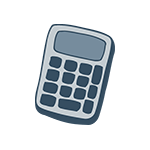
\includegraphics[scale=0.5]{MISC/calculator.png} };
 \end{tikzpicture} 
 }{
 \ifthenelse{\equal{#3}{2}}{
 \begin{tikzpicture}
 	\node[minimum width=0.7cm]{
\includegraphics[scale=0.5]{MISC/no_calculator.png} };
 \end{tikzpicture} 
 }{}
 }

\end{minipage}
\hfill
\begin{minipage}[t]{17.3cm}
} 
{ 
\end{minipage}%code  après
\hfill
\begin{minipage}[t]{1cm}

\begin{center}
\colorbox{sacado_violet}{
\includegraphics[height=1cm]{qrcodes/qrDummy.png}}
\colorbox{white}{ {\footnotesize /b/ABCD} }
\end{center}

\end{minipage}

\end{tcolorbox}
\par 
}

 
%%%%%%%%%%%%% ExoCu 7 paramètres : Compétences, qrcode , calculatrice, python, scratch, tableur, annales
\newenvironment{ExoCu}[7]{% code avant
\tcbset{top=-0.2cm }
\stepcounter{exo}

\begin{tcolorbox}[right=-5mm, enhanced, lifted shadow={0mm}{0mm}{0mm}{0mm}%
{black!60!white}, attach boxed title to top right={xshift=-0.3cm, yshift*=-2mm}, coltitle=sacado_green!85!black, colback=white!100!white, boxed title style={colback=white}, colframe=sacado_green!100!black,title= {\footnotesize  #1}  ]
 
\hspace{-1.3cm} 
\begin{minipage}[t]{0.7cm}

 \begin{tikzpicture}
 	\node[fill=sacado_green,minimum width=0.7cm]{\textcolor{white}{\bf {\Large \theexo}}};
 \end{tikzpicture}


%%%%%%%%%%%%%%%%%%%%%%%% Condition pour la calculatrice
 \ifthenelse{\equal{#3}{1}}{
 \begin{tikzpicture}
 	\node[minimum width=0.7cm]{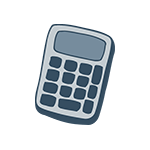
\includegraphics[scale=0.5]{MISC/calculator.png} };
 \end{tikzpicture} 
 }{
 \ifthenelse{\equal{#3}{2}}{
 \begin{tikzpicture}
 	\node[minimum width=0.7cm]{
\includegraphics[scale=0.5]{MISC/no_calculator.png} };
 \end{tikzpicture} 
 }{}
 }

\end{minipage}
\hfill
\begin{minipage}[t]{17.3cm}
} 
{ 
\end{minipage}%code  après
\hfill
\begin{minipage}[t]{1cm}

 
\begin{center}
\colorbox{sacado_green}{
\includegraphics[height=1cm]{qrcodes/qrDummy.png}}
\colorbox{white}{ {\footnotesize /b/ABCD}  }
\end{center}
 

\end{minipage}

\end{tcolorbox}
\par
}  


 %%%%%%%%%%%%% ExoCd 7 paramètres : Compétences, qrcode , calculatrice, python, scratch, tableur, annales
\newenvironment{ExoCd}[7]{% code avant
\tcbset{top=-0.2cm }
\stepcounter{exo}

\begin{tcolorbox}[right=-5mm, enhanced, lifted shadow={0mm}{0mm}{0mm}{0mm}%
{black!60!white}, attach boxed title to top right={xshift=-0.3cm, yshift*=-2mm}, coltitle=sacado_blue!85!black, colback=white!100!white, boxed title style={colback=white}, colframe=sacado_blue!100!black,title= {\footnotesize  #1}  ]
 
\hspace{-1.3cm} 
\begin{minipage}[t]{0.7cm}

 \begin{tikzpicture}
 	\node[fill=sacado_blue,minimum width=0.7cm]{\textcolor{white}{\bf {\Large \theexo}}};
 \end{tikzpicture}


%%%%%%%%%%%%%%%%%%%%%%%% Condition pour la calculatrice
 \ifthenelse{\equal{#3}{1}}{
 \begin{tikzpicture}
 	\node[minimum width=0.7cm]{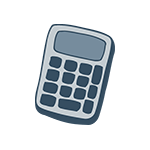
\includegraphics[scale=0.5]{MISC/calculator.png} };
 \end{tikzpicture} 
 }{
 \ifthenelse{\equal{#3}{2}}{
 \begin{tikzpicture}
 	\node[minimum width=0.7cm]{
\includegraphics[scale=0.5]{MISC/no_calculator.png} };
 \end{tikzpicture} 
 }{}
 }

\end{minipage}
\hfill
\begin{minipage}[t]{17.3cm}
} 
{ 
\end{minipage}%code  après
\hfill
\begin{minipage}[t]{1cm}

\begin{center}
\colorbox{sacado_blue}{
\includegraphics[height=1cm]{qrcodes/qrDummy.png}}
\colorbox{white}{ {\footnotesize /b/ABCD} }
\end{center}

\end{minipage}

\end{tcolorbox}
\par
}  


%%%%%%%%%%%%% ExoCt 7 paramètres : Compétences, qrcode , calculatrice, python, scratch, tableur, annales
\newenvironment{ExoCt}[7]{% code avant
\tcbset{top=-0.2cm }
\stepcounter{exo}

\begin{tcolorbox}[right=-5mm, enhanced, lifted shadow={0mm}{0mm}{0mm}{0mm}%
{black!60!white}, attach boxed title to top right={xshift=-0.3cm, yshift*=-2mm}, coltitle=sacado_red!85!black, colback=white!100!white, boxed title style={colback=white}, colframe=sacado_red!100!black,title= {\footnotesize  #1}  ]
 
\hspace{-1.3cm} 
\begin{minipage}[t]{0.7cm}

 \begin{tikzpicture}
 	\node[fill=sacado_red,minimum width=0.7cm]{\textcolor{white}{\bf {\Large \theexo}}};
 \end{tikzpicture}


%%%%%%%%%%%%%%%%%%%%%%%% Condition pour la calculatrice
 \ifthenelse{\equal{#3}{1}}{
 \begin{tikzpicture}
 	\node[minimum width=0.7cm]{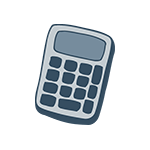
\includegraphics[scale=0.5]{MISC/calculator.png} };
 \end{tikzpicture} 
 }{
 \ifthenelse{\equal{#3}{2}}{
 \begin{tikzpicture}
 	\node[minimum width=0.7cm]{
\includegraphics[scale=0.5]{MISC/no_calculator.png} };
 \end{tikzpicture} 
 }{}
 }

\end{minipage}
\hfill
\begin{minipage}[t]{17.3cm}
} 
{ 
\end{minipage}%code  après
\hfill
\begin{minipage}[t]{1cm}

\begin{center}
\colorbox{sacado_red}{
\includegraphics[height=1cm]{qrcodes/qrDummy.png}}
\colorbox{white}{ {\footnotesize /b/ABCD} }
\end{center}

\end{minipage}

\end{tcolorbox}
\par
}  

 
 
 

%%%%%%%%%%%%% ExoCu 7 paramètres : compétences , qrcode , calculatrice, python, scratch, tableur, annales
\newenvironment{ExoAuto}[7]{% code avant
\tcbset{top=-0.2cm }
\stepcounter{exo}

\begin{tcolorbox}[right=-5mm, enhanced, lifted shadow={0mm}{0mm}{0mm}{0mm}%
{black!60!white}, attach boxed title to top right={xshift=-0.3cm, yshift*=-2mm}, coltitle=sacado_orange!85!black, colback=white!100!white, boxed title style={colback=white}, colframe=sacado_orange!100!black,title= {\footnotesize  #1}  ]
 
\hspace{-1.3cm} 
\begin{minipage}[t]{0.7cm}

 \begin{tikzpicture}
 	\node[fill=sacado_orange,minimum width=0.7cm]{\textcolor{white}{\bf {\Large \theexo}}};
 \end{tikzpicture}


%%%%%%%%%%%%%%%%%%%%%%%% Condition pour la calculatrice
 \ifthenelse{\equal{#3}{1}}{
 \begin{tikzpicture}
 	\node[minimum width=0.7cm]{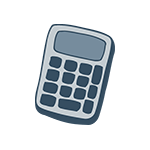
\includegraphics[scale=0.5]{MISC/calculator.png} };
 \end{tikzpicture} 
 }{
 \ifthenelse{\equal{#3}{2}}{
 \begin{tikzpicture}
 	\node[minimum width=0.7cm]{
\includegraphics[scale=0.5]{MISC/no_calculator.png} };
 \end{tikzpicture} 
 }{}
 }

\end{minipage}
\hfill
\begin{minipage}[t]{17.3cm}
} 
{ 
\end{minipage}%code  après
\hfill
\begin{minipage}[t]{1cm}

\begin{center}
\colorbox{sacado_orange}{
\includegraphics[height=1cm]{qrcodes/qrDummy.png}}
\colorbox{white}{  {\footnotesize /b/ABCD}  }
\end{center}

\end{minipage}

\end{tcolorbox}
\par
}  

 

%%%%%%%%%%%%% ExoDec 7 paramètres : compétences , qrcode , calculatrice, python, scratch, tableur, annales
 
\newenvironment{ExoDec}[6]{% code avant
\tcbset{top=-0.2cm }
\stepcounter{exo}

\begin{tcolorbox}[right=-5mm, enhanced, lifted shadow={0mm}{0mm}{0mm}{0mm}%
{black!60!white}, attach boxed title to top right={xshift=-0.3cm, yshift*=-2mm}, coltitle=sacado_violet!85!black, colback=white!100!white, boxed title style={colback=white}, colframe=sacado_violet!100!black,title= {\footnotesize  #1}  ]
 
\hspace{-1.3cm} 
\begin{minipage}[t]{1cm}

 \begin{tikzpicture}
 	\node[fill=sacado_violet,minimum width=0.7cm]{\textcolor{white}{\bf {\Large \theexo}}};
 \end{tikzpicture}


%%%%%%%%%%%%%%%%%%%%%%%% Condition pour la calculatrice
 \ifthenelse{\equal{#3}{1}}{
 \begin{tikzpicture}
 	\node[minimum width=0.7cm]{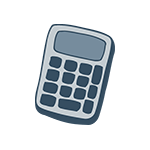
\includegraphics[scale=0.5]{MISC/calculator.png} };
 \end{tikzpicture} 
 }{
 \ifthenelse{\equal{#3}{2}}{
 \begin{tikzpicture}
 	\node[minimum width=0.7cm]{
\includegraphics[scale=0.5]{MISC/no_calculator.png} };
 \end{tikzpicture} 
 }{}
 }

\end{minipage}
\begin{minipage}[t]{17.3cm}
} 
{ 
\end{minipage}
\end{tcolorbox}
\par
}  
%%%%%%%%%%%%%%%%%%%%%%%%%%%%%%%%%%%%%%%%%%%%%%%%%%%%%%%%%%%%%%%%%%%%%%%%%%%%%%%%%%%%%%%%%%%%%%%%%%%%%%%%%%%%%%%%%%%%%%
%%%%%%%%%%%%%%%%%%%%%%%%%%%%%%%%%%%%%%%%%%%%%%%%%%%%%%%%%%%%%%%%%%%%%%%%%%%%%%%%%%%%%%%%%%%%%%%%%%%%%%%%%%%%%%%%%%%%%%
%%%%%%%%%%%%%%%%  Exercices sans qrcode                                %%%%%%%%%%%%%%%%%%%%%%%%%%%%%%%%%%%%%%%%%%%%%%%
%%%%%%%%%%%%%%%%%%%%%%%%%%%%%%%%%%%%%%%%%%%%%%%%%%%%%%%%%%%%%%%%%%%%%%%%%%%%%%%%%%%%%%%%%%%%%%%%%%%%%%%%%%%%%%%%%%%%%%
%%%%%%%%%%%%%%%%%%%%%%%%%%%%%%%%%%%%%%%%%%%%%%%%%%%%%%%%%%%%%%%%%%%%%%%%%%%%%%%%%%%%%%%%%%%%%%%%%%%%%%%%%%%%%%%%%%%%%%
 
 
 
%%%%%%%%%%%%% ExoCad 7 paramètres : Compétences , calculatrice, python, scratch, tableur, annales
\newenvironment{ExoCadN}[6]{% code avant
\tcbset{top=-0.2cm }
\stepcounter{exo}

\begin{tcolorbox}[right=-5mm, enhanced, lifted shadow={0mm}{0mm}{0mm}{0mm}%
{black!60!white}, attach boxed title to top right={xshift=-0.3cm, yshift*=-2mm}, coltitle=sacado_violet!85!black, colback=white!100!white, boxed title style={colback=white}, colframe=sacado_violet!100!black,title= {\footnotesize  #1}  ]
 
\hspace{-1.3cm} 
\begin{minipage}[t]{1cm}

 \begin{tikzpicture}
 	\node[fill=sacado_violet,minimum width=0.7cm]{\textcolor{white}{\bf {\Large \theexo}}};
 \end{tikzpicture}


%%%%%%%%%%%%%%%%%%%%%%%% Condition pour la calculatrice
 \ifthenelse{\equal{#3}{1}}{
 \begin{tikzpicture}
 	\node[minimum width=0.7cm]{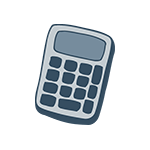
\includegraphics[scale=0.5]{MISC/calculator.png} };
 \end{tikzpicture} 
 }{
 \ifthenelse{\equal{#3}{2}}{
 \begin{tikzpicture}
 	\node[minimum width=0.7cm]{
\includegraphics[scale=0.5]{MISC/no_calculator.png} };
 \end{tikzpicture} 
 }{}
 }

\end{minipage}
\begin{minipage}[t]{17.3cm}
} 
{ 
\end{minipage}%code  après
\end{tcolorbox}
\par 
}

 
%%%%%%%%%%%%% ExoCu 7 paramètres : Compétences , calculatrice, python, scratch, tableur, annales
\newenvironment{ExoCuN}[6]{% code avant
\tcbset{top=-0.2cm }
\stepcounter{exo}

\begin{tcolorbox}[right=-5mm, enhanced, lifted shadow={0mm}{0mm}{0mm}{0mm}%
{black!60!white}, attach boxed title to top right={xshift=-0.3cm, yshift*=-2mm}, coltitle=sacado_green!85!black, colback=white!100!white, boxed title style={colback=white}, colframe=sacado_green!100!black,title= {\footnotesize  #1}  ]
 
\hspace{-1.3cm} 
\begin{minipage}[t]{1cm}

 \begin{tikzpicture}
 	\node[fill=sacado_green,minimum width=0.7cm]{\textcolor{white}{\bf {\Large \theexo}}};
 \end{tikzpicture}


%%%%%%%%%%%%%%%%%%%%%%%% Condition pour la calculatrice
 \ifthenelse{\equal{#2}{1}}{
 \begin{tikzpicture}
 	\node[minimum width=0.7cm]{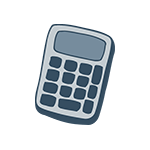
\includegraphics[scale=0.5]{MISC/calculator.png} };
 \end{tikzpicture} 
 }{
 \ifthenelse{\equal{#2}{2}}{
 \begin{tikzpicture}
 	\node[minimum width=0.7cm]{
\includegraphics[scale=0.5]{MISC/no_calculator.png} };
 \end{tikzpicture} 
 }{}
 }

\end{minipage}
\begin{minipage}[t]{17.3cm}
} 
{ 
\end{minipage}
\end{tcolorbox}
\par
}  


 %%%%%%%%%%%%% ExoCd 6 paramètres : Compétences, calculatrice, python, scratch, tableur, annales
\newenvironment{ExoCdN}[6]{% code avant
\tcbset{top=-0.2cm }
\stepcounter{exo}

\begin{tcolorbox}[right=-5mm, enhanced, lifted shadow={0mm}{0mm}{0mm}{0mm}%
{black!60!white}, attach boxed title to top right={xshift=-0.3cm, yshift*=-2mm}, coltitle=sacado_blue!85!black, colback=white!100!white, boxed title style={colback=white}, colframe=sacado_blue!100!black,title= {\footnotesize  #1}  ]
 
\hspace{-1.3cm} 
\begin{minipage}[t]{1cm}

 \begin{tikzpicture}
 	\node[fill=sacado_blue,minimum width=0.7cm]{\textcolor{white}{\bf {\Large \theexo}}};
 \end{tikzpicture}


%%%%%%%%%%%%%%%%%%%%%%%% Condition pour la calculatrice
 \ifthenelse{\equal{#2}{1}}{
 \begin{tikzpicture}
 	\node[minimum width=0.7cm]{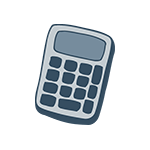
\includegraphics[scale=0.5]{MISC/calculator.png} };
 \end{tikzpicture} 
 }{
 \ifthenelse{\equal{#2}{2}}{
 \begin{tikzpicture}
 	\node[minimum width=0.7cm]{
\includegraphics[scale=0.5]{MISC/no_calculator.png} };
 \end{tikzpicture} 
 }{}
 }

\end{minipage}
\begin{minipage}[t]{17.3cm}
} 
{ 
\end{minipage}%code  après
\end{tcolorbox}
\par
}  


%%%%%%%%%%%%% ExoCt 6 paramètres : Compétences,   calculatrice, python, scratch, tableur, annales
\newenvironment{ExoCtN}[6]{% code avant
\tcbset{top=-0.2cm }
\stepcounter{exo}

\begin{tcolorbox}[right=-5mm, enhanced, lifted shadow={0mm}{0mm}{0mm}{0mm}%
{black!60!white}, attach boxed title to top right={xshift=-0.3cm, yshift*=-2mm}, coltitle=sacado_red!85!black, colback=white!100!white, boxed title style={colback=white}, colframe=sacado_red!100!black,title= {\footnotesize  #1}  ]
 
\hspace{-1.3cm} 
\begin{minipage}[t]{1cm}

 \begin{tikzpicture}
 	\node[fill=sacado_red,minimum width=0.7cm]{\textcolor{white}{\bf {\Large \theexo}}};
 \end{tikzpicture}


%%%%%%%%%%%%%%%%%%%%%%%% Condition pour la calculatrice
 \ifthenelse{\equal{#2}{1}}{
 \begin{tikzpicture}
 	\node[minimum width=0.7cm]{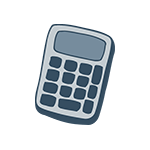
\includegraphics[scale=0.5]{MISC/calculator.png} };
 \end{tikzpicture} 
 }{
 \ifthenelse{\equal{#2}{2}}{
 \begin{tikzpicture}
 	\node[minimum width=0.7cm]{
\includegraphics[scale=0.5]{MISC/no_calculator.png} };
 \end{tikzpicture} 
 }{}
 }

\end{minipage}
\begin{minipage}[t]{17.3cm}
} 
{ 
\end{minipage}%code  après
\end{tcolorbox}
\par
}  

 
 
 

%%%%%%%%%%%%% ExoCu 7 paramètres : compétences , qrcode , calculatrice, python, scratch, tableur, annales
\newenvironment{ExoAutoN}[6]{% code avant
\tcbset{top=-0.2cm }
\stepcounter{exo}

\begin{tcolorbox}[right=5mm, enhanced, lifted shadow={0mm}{0mm}{0mm}{0mm}%
{black!60!white}, attach boxed title to top right={xshift=-0.3cm, yshift*=-2mm}, coltitle=sacado_orange!85!black, colback=white!100!white, boxed title style={colback=white}, colframe=sacado_orange!100!black,title= {\footnotesize  #1}  ]
 
\hspace{-1.4cm} 
\begin{minipage}[t]{0.7cm}

 \begin{tikzpicture}
 	\node[fill=sacado_orange,minimum width=0.7cm]{\textcolor{white}{\bf {\Large \theexo}}};
 \end{tikzpicture}


%%%%%%%%%%%%%%%%%%%%%%%% Condition pour la calculatrice
 \ifthenelse{\equal{#2}{1}}{
 \begin{tikzpicture}
 	\node[minimum width=0.7cm]{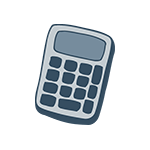
\includegraphics[scale=0.5]{MISC/calculator.png} };
 \end{tikzpicture} 
 }{
 \ifthenelse{\equal{#2}{2}}{
 \begin{tikzpicture}
 	\node[minimum width=0.7cm]{
\includegraphics[scale=0.5]{MISC/no_calculator.png} };
 \end{tikzpicture} 
 }{}
 }

\end{minipage}
\hfill
\begin{minipage}[t]{17.3cm}
} 
{ 
\end{minipage}%code  après
\end{tcolorbox}
\par
}  
%%%%%%%%%%%%%%%%%%%%%%%%%%%%%%%%%%%%%%%%%%%%%%%%%%%%%%%%%%%%%%%%%%%%%%%%%%%%%%%%%%%%%%%%%%%%%%%%%%%%%%%%%%%%%%%%%%%%%%
%%%%%%%%%%%%%%%%%%%%%%%%%%%%%%%%%%%%%%%%%%%%%%%%%%%%%%%%%%%%%%%%%%%%%%%%%%%%%%%%%%%%%%%%%%%%%%%%%%%%%%%%%%%%%%%%%%%%%%
%%%%%%%%%%%%%%%%  Exercices   sans contours                            %%%%%%%%%%%%%%%%%%%%%%%%%%%%%%%%%%%%%%%%%%%%%%%
%%%%%%%%%%%%%%%%%%%%%%%%%%%%%%%%%%%%%%%%%%%%%%%%%%%%%%%%%%%%%%%%%%%%%%%%%%%%%%%%%%%%%%%%%%%%%%%%%%%%%%%%%%%%%%%%%%%%%%
%%%%%%%%%%%%%%%%%%%%%%%%%%%%%%%%%%%%%%%%%%%%%%%%%%%%%%%%%%%%%%%%%%%%%%%%%%%%%%%%%%%%%%%%%%%%%%%%%%%%%%%%%%%%%%%%%%%%%%


\newcommand{\Sf}[1]{ \vspace{0.1cm}
{\color{fond}{\Large \textbf{#1}}  } 
} 

\newcommand{\Sfe}[1]{ \vspace{0.1cm}
{\color{sacado_blue}{\Large \textbf{#1}}  } 
} 
% fin de la procédure



%%%%%%%%%%%%% Pointillés ou ligne
\newcommand{\point}[1]{\vspace{0.1cm}\multido{}{#1}{ \dotfill \medskip \endgraf}}
\newcommand{\ligne}[1]{\vspace{0.1cm}\multido{}{#1}{ {\color{cqcqcq}\hrulefill} \medskip \endgraf}}
%----------------------------------------
%
%   Macros et opérateurs
%
%----------------------------------------

\newcommand{\second}{2\up{d}\xspace}
\newcommand{\seconde}{2\up{de}\xspace}
\newcommand{\R}{\mathbb R}
\newcommand{\Rp}{\R_+}
\newcommand{\Rpe}{\R_+^*}
\newcommand{\Rm}{\R_-}
\newcommand{\Rme}{\R_-^*}
\newcommand{\N}{\mathbb N}
\newcommand{\D}{\mathbb D}
\newcommand{\Q}{\mathbb Q}
\newcommand{\Z}{\mathbb Z}
\newcommand{\C}{\mathbb C}
\newcommand{\grs}{\mathfrak S}
\newcommand{\IN}[1]{\llbracket 1,#1\rrbracket}
\newcommand{\card}{\text{Card}\,}
\usepackage{mathrsfs}
\newcommand{\parties}{\mathscr P}
\renewcommand{\epsilon}{\varepsilon}
\newcommand{\rmd}{\text{d}}
\newcommand{\diff}{\mathrm D}
\newcommand{\Id}{{\rm Id}}
\newcommand{\e}{{\rm e}}
\newcommand{\I}{{\rm i}}
\newcommand{\J}{{\rm j}}
\newcommand{\ro}{\circ}
\newcommand{\exu}{\exists\,!\,}
\newcommand{\telq}{\,\, \mid \,\,}
\newcommand{\para}{\raisebox{0.1em}{\text{\footnotesize /\hspace{-0.1em}/}}}   
\newcommand{\vect}[1]{\overrightarrow{#1}}
\newcommand{\scal}[2]{\left(\, #1 \mid #2 \, \right)}
\newcommand{\ortho}[1]{{#1}^\perp}
\newcommand{\veci}{\vec{\text{\it \i}}}
\newcommand{\vecj}{\vec{\text{\it \j}}}
\newcommand{\rep}{$(O;\veci,\vecj,\vec{k})$\xspace}
\newcommand{\Oijk}{$(O, \veci,\vecj,\vec{k})$\xspace}
\newcommand{\rond}{repère orthonormal direct}
\newcommand{\bond}{base orthonormale directe}
\newcommand{\eq}{\Longleftrightarrow}
\newcommand{\implique}{\Longrightarrow}
\newcommand{\noneq}{\ \ \ /\hspace{-1.45em}\eq}
\newcommand{\tend}{\longrightarrow}
\newcommand{\egx}[2]{\underset{#1 \tend #2}=}
\newcommand{\asso}{\longmapsto}
\newcommand{\vers}{\longrightarrow}
\newcommand{\eqn}{~\underset{n \rightarrow \infty}{\sim}~}
\newcommand{\eqx}[2]{~\underset{#1 \rightarrow #2}{\sim}~}

\newcommand{\egn}{~\underset{n \rightarrow \infty}{=}~}
\renewcommand{\descriptionlabel}{\hspace{\labelsep}$\bullet$}
\renewcommand{\bar}{\overline}
\DeclareMathOperator{\ash}{{Argsh}}
\DeclareMathOperator{\cotan}{{cotan}}
\DeclareMathOperator{\ach}{{Argch}}
\DeclareMathOperator{\ath}{{Argth}}
\DeclareMathOperator{\sh}{{sh}}
\DeclareMathOperator{\ch}{{ch}}
\DeclareMathOperator{\Mat}{{Mat}}
\DeclareMathOperator{\Vect}{{Vect}}
\DeclareMathOperator{\trace}{{tr}}
\newcommand{\tr}{{}^{\mathrm t}}
\newcommand{\divi}{~\big|~}
\newcommand{\ndivi}{~\not{\big|}~}
\newcommand{\et}{\wedge}
\newcommand{\ou}{\vee}
\renewcommand{\det}{\operatorname{\text{dét}}}
\DeclareMathOperator{\grad}{{grad}}
\renewcommand{\arcsin}{{\mathop{\mathrm{Arcsin}}}}
\renewcommand{\arccos}{{\mathop{\mathrm{Arccos}}}}
\renewcommand{\arctan}{{\mathop{\mathrm{Arctan}}}}
\renewcommand{\tanh}{{\mathop{\mathrm{th}}}}
\newcommand{\pgcd}{\mathop{\mathrm{pgcd}}}
\newcommand{\ppcm}{\mathop{\mathrm{ppcm}}}
\newcommand{\fonc}[4]{\left\{\begin{tabular}{ccc}$#1$ & $\vers$ & $#2$ \\
$#3$ & $\asso$ & $#4$ \end{tabular}\right.}
\renewcommand{\geq}{\geqslant}
\renewcommand{\leq}{\leqslant}
\renewcommand{\Re}{\text{\rm Re}}
\renewcommand{\Im}{\text{\rm Im}}
\renewcommand{\ker}{\mathop{\mathrm{Ker}}}
\newcommand{\Lin}{\mathcal L}
\newcommand{\GO}{\mathcal O}
\newcommand{\GSO}{\mathcal{SO}}
\newcommand{\GL}{\mathcal{GL}}
\renewcommand{\emptyset}{\varnothing}
%\newcommand{\arc}[1]{\overset{\frown}{#1}}
\newcommand{\rg}{\mathop{\mathrm{rg}}}
\newcommand{\ds}{\displaystyle}
\newcommand{\co}[3]{\begin{pmatrix}#1 \\ #2 \\ #3\end{pmatrix}}
\newcommand{\demi}{\frac 1 2}
\newcommand{\limi}[2]{\underset{#1 \rightarrow #2}\lim}
%\usetikzlibrary{quotes,arrows.meta}
% Pour les pavés droits sans annotations de hLl 
\tikzset{
  nonannotated cuboid/.pic={
    \tikzset{%
      every edge quotes/.append style={midway, auto},
      /cuboid/.cd,
      #1
    }
    \draw [every edge/.append style={pic actions, densely dashed, opacity=.5}, pic actions]
    (0,0,0) coordinate (o) -- ++(-\cubescale*\cubex,0,0) coordinate (a) -- ++(0,-\cubescale*\cubey,0) coordinate (b) edge coordinate [pos=1] (g) ++(0,0,-\cubescale*\cubez)  -- ++(\cubescale*\cubex,0,0) coordinate (c) -- cycle
    (o) -- ++(0,0,-\cubescale*\cubez) coordinate (d) -- ++(0,-\cubescale*\cubey,0) coordinate (e) edge (g) -- (c) -- cycle
    (o) -- (a) -- ++(0,0,-\cubescale*\cubez) coordinate (f) edge (g) -- (d) -- cycle;
%    \path [every edge/.append style={pic actions, |-|}]
%    (b) +(0,-5pt) coordinate (b1) edge ["\cubex \cubeunits"'] (b1 -| c)
%    (b) +(-5pt,0) coordinate (b2) edge ["\cubey \cubeunits"] (b2 |- a)
%    (c) +(3.5pt,-3.5pt) coordinate (c2) edge ["\cubez \cubeunits"'] ([xshift=3.5pt,yshift=-3.5pt]e)
    ;
  },
  /cuboid/.search also={/tikz},
  /cuboid/.cd,
  width/.store in=\cubex,
  height/.store in=\cubey,
  depth/.store in=\cubez,
  units/.store in=\cubeunits,
  scale/.store in=\cubescale,
  width=10,
  height=10,
  depth=10,
  units=cm,
  scale=.1,
}

% Pour les pavés droits avec annotations de hLl
\tikzset{
  annotated cuboid/.pic={
    \tikzset{%
      every edge quotes/.append style={midway, auto},
      /cuboid/.cd,
      #1
    }
    \draw [every edge/.append style={pic actions, densely dashed, opacity=.5}, pic actions]
    (0,0,0) coordinate (o) -- ++(-\cubescale*\cubex,0,0) coordinate (a) -- ++(0,-\cubescale*\cubey,0) coordinate (b) edge coordinate [pos=1] (g) ++(0,0,-\cubescale*\cubez)  -- ++(\cubescale*\cubex,0,0) coordinate (c) -- cycle
    (o) -- ++(0,0,-\cubescale*\cubez) coordinate (d) -- ++(0,-\cubescale*\cubey,0) coordinate (e) edge (g) -- (c) -- cycle
    (o) -- (a) -- ++(0,0,-\cubescale*\cubez) coordinate (f) edge (g) -- (d) -- cycle;
    \path [every edge/.append style={pic actions, |-|}]
    (b) +(0,-5pt) coordinate (b1) edge ["\cubex \cubeunits"'] (b1 -| c)
    (b) +(-5pt,0) coordinate (b2) edge ["\cubey \cubeunits"] (b2 |- a)
    (c) +(3.5pt,-3.5pt) coordinate (c2) edge ["\cubez \cubeunits"'] ([xshift=3.5pt,yshift=-3.5pt]e)
    ;
  },
  /cuboid/.search also={/tikz},
  /cuboid/.cd,
  width/.store in=\cubex,
  height/.store in=\cubey,
  depth/.store in=\cubez,
  units/.store in=\cubeunits,
  scale/.store in=\cubescale,
  width=10,
  height=10,
  depth=10,
  units=cm,
  scale=.1,
}

% Pour les pavés droits avec annotations "hauteur", "Longueur", "largeur".
\tikzset{
  defannotated cuboid/.pic={
    \tikzset{%
      every edge quotes/.append style={midway, auto},
      /cuboid/.cd,
      #1
    }
    \draw [every edge/.append style={pic actions, densely dashed, opacity=.5}, pic actions]
    (0,0,0) coordinate (o) -- ++(-\cubescale*\cubex,0,0) coordinate (a) -- ++(0,-\cubescale*\cubey,0) coordinate (b) edge coordinate [pos=1] (g) ++(0,0,-\cubescale*\cubez)  -- ++(\cubescale*\cubex,0,0) coordinate (c) -- cycle
    (o) -- ++(0,0,-\cubescale*\cubez) coordinate (d) -- ++(0,-\cubescale*\cubey,0) coordinate (e) edge (g) -- (c) -- cycle
    (o) -- (a) -- ++(0,0,-\cubescale*\cubez) coordinate (f) edge (g) -- (d) -- cycle;
    \path [every edge/.append style={pic actions, |-|}]
    (b) +(0,-5pt) coordinate (b1) edge ["Longueur"'] (b1 -| c)
    (b) +(-5pt,0) coordinate (b2) edge ["Hauteur"] (b2 |- a)
    (c) +(3.5pt,-3.5pt) coordinate (c2) edge ["largeur"'] ([xshift=3.5pt,yshift=-3.5pt]e)
    ;
  },
  /cuboid/.search also={/tikz},
  /cuboid/.cd,
  width/.store in=\cubex,
  height/.store in=\cubey,
  depth/.store in=\cubez,
  units/.store in=\cubeunits,
  scale/.store in=\cubescale,
  width=10,
  height=10,
  depth=10,
  units=cm,
  scale=.1,
}

\tikzset{
  defiannotated cuboid/.pic={
    \tikzset{%
      every edge quotes/.append style={midway, auto},
      /cuboid/.cd,
      #1
    }
    \draw [every edge/.append style={pic actions, densely dashed, opacity=.5}, pic actions]
    (0,0,0) coordinate (o) -- ++(-\cubescale*\cubex,0,0) coordinate (a) -- ++(0,-\cubescale*\cubey,0) coordinate (b) edge coordinate [pos=1] (g) ++(0,0,-\cubescale*\cubez)  -- ++(\cubescale*\cubex,0,0) coordinate (c) -- cycle
    (o) -- ++(0,0,-\cubescale*\cubez) coordinate (d) -- ++(0,-\cubescale*\cubey,0) coordinate (e) edge (g) -- (c) -- cycle
    (o) -- (a) -- ++(0,0,-\cubescale*\cubez) coordinate (f) edge (g) -- (d) -- cycle;
    \path [every edge/.append style={pic actions, |-|}]
    (b) +(0,-5pt) coordinate (b1) edge ["c"'] (b1 -| c)
    (b) +(-5pt,0) coordinate (b2) edge ["c"] (b2 |- a)
    (c) +(3.5pt,-3.5pt) coordinate (c2) edge ["c"'] ([xshift=3.5pt,yshift=-3.5pt]e)
    ;
  },
  /cuboid/.search also={/tikz},
  /cuboid/.cd,
  width/.store in=\cubex,
  height/.store in=\cubey,
  depth/.store in=\cubez,
  units/.store in=\cubeunits,
  scale/.store in=\cubescale,
  width=10,
  height=10,
  depth=10,
  units=cm,
  scale=.1,
}

\tikzset{
  defiiannotated cuboid/.pic={
    \tikzset{%
      every edge quotes/.append style={midway, auto},
      /cuboid/.cd,
      #1
    }
    \draw [every edge/.append style={pic actions, densely dashed, opacity=.5}, pic actions]
    (0,0,0) coordinate (o) -- ++(-\cubescale*\cubex,0,0) coordinate (a) -- ++(0,-\cubescale*\cubey,0) coordinate (b) edge coordinate [pos=1] (g) ++(0,0,-\cubescale*\cubez)  -- ++(\cubescale*\cubex,0,0) coordinate (c) -- cycle
    (o) -- ++(0,0,-\cubescale*\cubez) coordinate (d) -- ++(0,-\cubescale*\cubey,0) coordinate (e) edge (g) -- (c) -- cycle
    (o) -- (a) -- ++(0,0,-\cubescale*\cubez) coordinate (f) edge (g) -- (d) -- cycle;
    \path [every edge/.append style={pic actions, |-|}]
    (b) +(0,-5pt) coordinate (b1) edge ["L"'] (b1 -| c)
    (b) +(-5pt,0) coordinate (b2) edge ["h"] (b2 |- a)
    (c) +(3.5pt,-3.5pt) coordinate (c2) edge ["l"'] ([xshift=3.5pt,yshift=-3.5pt]e)
    ;
  },
  /cuboid/.search also={/tikz},
  /cuboid/.cd,
  width/.store in=\cubex,
  height/.store in=\cubey,
  depth/.store in=\cubez,
  units/.store in=\cubeunits,
  scale/.store in=\cubescale,
  width=10,
  height=10,
  depth=10,
  units=cm,
  scale=.1,
}

\tikzset{
  xannotated cuboid/.pic={
    \tikzset{%
      every edge quotes/.append style={midway, auto},
      /cuboid/.cd,
      #1
    }
    \draw [every edge/.append style={pic actions, densely dashed, opacity=.5}, pic actions]
    (0,0,0) coordinate (o) -- ++(-\cubescale*\cubex,0,0) coordinate (a) -- ++(0,-\cubescale*\cubey,0) coordinate (b) edge coordinate [pos=1] (g) ++(0,0,-\cubescale*\cubez)  -- ++(\cubescale*\cubex,0,0) coordinate (c) -- cycle
    (o) -- ++(0,0,-\cubescale*\cubez) coordinate (d) -- ++(0,-\cubescale*\cubey,0) coordinate (e) edge (g) -- (c) -- cycle
    (o) -- (a) -- ++(0,0,-\cubescale*\cubez) coordinate (f) edge (g) -- (d) -- cycle;
    \path [every edge/.append style={pic actions, |-|}]
    (b) +(0,-5pt) coordinate (b1) edge ["1cm"'] (b1 -| c)
    (b) +(-5pt,0) coordinate (b2) edge ["1cm"] (b2 |- a)
    (c) +(3.5pt,-3.5pt) coordinate (c2) edge ["1cm"'] ([xshift=3.5pt,yshift=-3.5pt]e)
    ;
  },
  /cuboid/.search also={/tikz},
  /cuboid/.cd,
  width/.store in=\cubex,
  height/.store in=\cubey,
  depth/.store in=\cubez,
  units/.store in=\cubeunits,
  scale/.store in=\cubescale,
  width=10,
  height=10,
  depth=10,
  units=cm,
  scale=.1,
}

\tikzset{
  yannotated cuboid/.pic={
    \tikzset{%
      every edge quotes/.append style={midway, auto},
      /cuboid/.cd,
      #1
    }
    \draw [every edge/.append style={pic actions, densely dashed, opacity=.5}, pic actions]
    (0,0,0) coordinate (o) -- ++(-\cubescale*\cubex,0,0) coordinate (a) -- ++(0,-\cubescale*\cubey,0) coordinate (b) edge coordinate [pos=1] (g) ++(0,0,-\cubescale*\cubez)  -- ++(\cubescale*\cubex,0,0) coordinate (c) -- cycle
    (o) -- ++(0,0,-\cubescale*\cubez) coordinate (d) -- ++(0,-\cubescale*\cubey,0) coordinate (e) edge (g) -- (c) -- cycle
    (o) -- (a) -- ++(0,0,-\cubescale*\cubez) coordinate (f) edge (g) -- (d) -- cycle;
    \path [every edge/.append style={pic actions, |-|}]
    (b) +(0,-5pt) coordinate (b1) edge ["1mm"'] (b1 -| c)
    (b) +(-5pt,0) coordinate (b2) edge ["1mm"] (b2 |- a)
    (c) +(3.5pt,-3.5pt) coordinate (c2) edge ["1mm"'] ([xshift=3.5pt,yshift=-3.5pt]e)
    ;
  },
  /cuboid/.search also={/tikz},
  /cuboid/.cd,
  width/.store in=\cubex,
  height/.store in=\cubey,
  depth/.store in=\cubez,
  units/.store in=\cubeunits,
  scale/.store in=\cubescale,
  width=10,
  height=10,
  depth=10,
  units=cm,
  scale=.1,
}

%Cubes subdivisés
\newif\ifcuboidshade
\newif\ifcuboidemphedge

\tikzset{
  cuboid/.is family,
  cuboid,
  shiftx/.initial=0,
  shifty/.initial=0,
  dimx/.initial=3,
  dimy/.initial=3,
  dimz/.initial=3,
  scale/.initial=1,
  densityx/.initial=1,
  densityy/.initial=1,
  densityz/.initial=1,
  rotation/.initial=0,
  anglex/.initial=0,
  angley/.initial=90,
  anglez/.initial=225,
  scalex/.initial=1,
  scaley/.initial=1,
  scalez/.initial=0.5,
  front/.style={draw=black,fill=white},
  top/.style={draw=black,fill=white},
  right/.style={draw=black,fill=white},
  shade/.is if=cuboidshade,
  shadecolordark/.initial=black,
  shadecolorlight/.initial=white,
  shadeopacity/.initial=0.15,
  shadesamples/.initial=16,
  emphedge/.is if=cuboidemphedge,
  emphstyle/.style={thick},
}

\newcommand{\tikzcuboidkey}[1]{\pgfkeysvalueof{/tikz/cuboid/#1}}

% Commands
\newcommand{\tikzcuboid}[1]{
    \tikzset{cuboid,#1} % Process Keys passed to command
  \pgfmathsetlengthmacro{\vectorxx}{\tikzcuboidkey{scalex}*cos(\tikzcuboidkey{anglex})*28.452756}
  \pgfmathsetlengthmacro{\vectorxy}{\tikzcuboidkey{scalex}*sin(\tikzcuboidkey{anglex})*28.452756}
  \pgfmathsetlengthmacro{\vectoryx}{\tikzcuboidkey{scaley}*cos(\tikzcuboidkey{angley})*28.452756}
  \pgfmathsetlengthmacro{\vectoryy}{\tikzcuboidkey{scaley}*sin(\tikzcuboidkey{angley})*28.452756}
  \pgfmathsetlengthmacro{\vectorzx}{\tikzcuboidkey{scalez}*cos(\tikzcuboidkey{anglez})*28.452756}
  \pgfmathsetlengthmacro{\vectorzy}{\tikzcuboidkey{scalez}*sin(\tikzcuboidkey{anglez})*28.452756}
  \begin{scope}[xshift=\tikzcuboidkey{shiftx}, yshift=\tikzcuboidkey{shifty}, scale=\tikzcuboidkey{scale}, rotate=\tikzcuboidkey{rotation}, x={(\vectorxx,\vectorxy)}, y={(\vectoryx,\vectoryy)}, z={(\vectorzx,\vectorzy)}]
    \pgfmathsetmacro{\steppingx}{1/\tikzcuboidkey{densityx}}
  \pgfmathsetmacro{\steppingy}{1/\tikzcuboidkey{densityy}}
  \pgfmathsetmacro{\steppingz}{1/\tikzcuboidkey{densityz}}
  \newcommand{\dimx}{\tikzcuboidkey{dimx}}
  \newcommand{\dimy}{\tikzcuboidkey{dimy}}
  \newcommand{\dimz}{\tikzcuboidkey{dimz}}
  \pgfmathsetmacro{\secondx}{2*\steppingx}
  \pgfmathsetmacro{\secondy}{2*\steppingy}
  \pgfmathsetmacro{\secondz}{2*\steppingz}
  \foreach \x in {\steppingx,\secondx,...,\dimx}
  { \foreach \y in {\steppingy,\secondy,...,\dimy}
    {   \pgfmathsetmacro{\lowx}{(\x-\steppingx)}
      \pgfmathsetmacro{\lowy}{(\y-\steppingy)}
      \filldraw[cuboid/front] (\lowx,\lowy,\dimz) -- (\lowx,\y,\dimz) -- (\x,\y,\dimz) -- (\x,\lowy,\dimz) -- cycle;
    }
    }
  \foreach \x in {\steppingx,\secondx,...,\dimx}
  { \foreach \z in {\steppingz,\secondz,...,\dimz}
    {   \pgfmathsetmacro{\lowx}{(\x-\steppingx)}
      \pgfmathsetmacro{\lowz}{(\z-\steppingz)}
      \filldraw[cuboid/top] (\lowx,\dimy,\lowz) -- (\lowx,\dimy,\z) -- (\x,\dimy,\z) -- (\x,\dimy,\lowz) -- cycle;
        }
    }
    \foreach \y in {\steppingy,\secondy,...,\dimy}
  { \foreach \z in {\steppingz,\secondz,...,\dimz}
    {   \pgfmathsetmacro{\lowy}{(\y-\steppingy)}
      \pgfmathsetmacro{\lowz}{(\z-\steppingz)}
      \filldraw[cuboid/right] (\dimx,\lowy,\lowz) -- (\dimx,\lowy,\z) -- (\dimx,\y,\z) -- (\dimx,\y,\lowz) -- cycle;
    }
  }
  \ifcuboidemphedge
    \draw[cuboid/emphstyle] (0,\dimy,0) -- (\dimx,\dimy,0) -- (\dimx,\dimy,\dimz) -- (0,\dimy,\dimz) -- cycle;%
    \draw[cuboid/emphstyle] (0,\dimy,\dimz) -- (0,0,\dimz) -- (\dimx,0,\dimz) -- (\dimx,\dimy,\dimz);%
    \draw[cuboid/emphstyle] (\dimx,\dimy,0) -- (\dimx,0,0) -- (\dimx,0,\dimz);%
    \fi

    \ifcuboidshade
    \pgfmathsetmacro{\cstepx}{\dimx/\tikzcuboidkey{shadesamples}}
    \pgfmathsetmacro{\cstepy}{\dimy/\tikzcuboidkey{shadesamples}}
    \pgfmathsetmacro{\cstepz}{\dimz/\tikzcuboidkey{shadesamples}}
    \foreach \s in {1,...,\tikzcuboidkey{shadesamples}}
    {   \pgfmathsetmacro{\lows}{\s-1}
        \pgfmathsetmacro{\cpercent}{(\lows)/(\tikzcuboidkey{shadesamples}-1)*100}
        \fill[opacity=\tikzcuboidkey{shadeopacity},color=\tikzcuboidkey{shadecolorlight}!\cpercent!\tikzcuboidkey{shadecolordark}] (0,\s*\cstepy,\dimz) -- (\s*\cstepx,\s*\cstepy,\dimz) -- (\s*\cstepx,0,\dimz) -- (\lows*\cstepx,0,\dimz) -- (\lows*\cstepx,\lows*\cstepy,\dimz) -- (0,\lows*\cstepy,\dimz) -- cycle;
        \fill[opacity=\tikzcuboidkey{shadeopacity},color=\tikzcuboidkey{shadecolorlight}!\cpercent!\tikzcuboidkey{shadecolordark}] (0,\dimy,\s*\cstepz) -- (\s*\cstepx,\dimy,\s*\cstepz) -- (\s*\cstepx,\dimy,0) -- (\lows*\cstepx,\dimy,0) -- (\lows*\cstepx,\dimy,\lows*\cstepz) -- (0,\dimy,\lows*\cstepz) -- cycle;
        \fill[opacity=\tikzcuboidkey{shadeopacity},color=\tikzcuboidkey{shadecolorlight}!\cpercent!\tikzcuboidkey{shadecolordark}] (\dimx,0,\s*\cstepz) -- (\dimx,\s*\cstepy,\s*\cstepz) -- (\dimx,\s*\cstepy,0) -- (\dimx,\lows*\cstepy,0) -- (\dimx,\lows*\cstepy,\lows*\cstepz) -- (\dimx,0,\lows*\cstepz) -- cycle;
    }
    \fi 

  \end{scope}
}

%\makeatother


\title{Mathématiques 6\ieme : le livre sacado}
\author{L'équipe SACADO}

\begin{document}

\parindent=0pt

\maketitle

%%-----------------------------
%%
%%   NOMBRES ET CALCULS
%%	/CHAPITRES/nombres_et_calculs
%%
%%-----------------------------
%
%% Additions et soustractions de nombres décimaux
%%-------------------------------
%	CONTENTS
%-------------------------------
\chapter{Additions et soustractions de nombres décimaux}
{https://sacado.xyz/qcm/parcours_show_course/0/117119}

\begin{pageCours} 

\section{Calculer un complément}

\begin{minipage}{0.6\linewidth}
\begin{Def}
Un \textbf{complément} est un nombre à \textbf{ajouter} pour atteindre un nombre donné.
\end{Def}

\begin{Ex}
Le complément à $314$ pour atteindre $1000$ est $686$
\[314+686=1000\]
\begin{description}
\item[]  $314 + 686 = 1000$
\item[] ou  $314 = 1000 - 686$
\end{description}
\end{Ex}

\end{minipage}
\begin{minipage}{0.4\linewidth}

\definecolor{wqwqwq}{rgb}{0.3764705882352941,0.3764705882352941,0.3764705882352941}
\definecolor{wwqqcc}{rgb}{0.4,0.,0.8}
\definecolor{ffwwqq}{rgb}{1.,0.4,0.}
\begin{tikzpicture}[line cap=round,line join=round,>=triangle 45,x=0.620970746495717cm,y=0.620970746495717cm]
\clip(-1.2872701767628254,1.716286654474951) rectangle (8.37502073445868,5.32161908403523);
\fill[line width=1.pt,color=ffwwqq,fill=ffwwqq,fill opacity=0.4] (-1.,5.) -- (2.,5.) -- (2.,4.) -- (-1.,4.) -- cycle;
\fill[line width=1.pt,color=wwqqcc,fill=wwqqcc,fill opacity=0.2] (2.,5.) -- (8.,5.) -- (8.,4.) -- (2.,4.) -- cycle;
\fill[line width=1.pt,dash pattern=on 1pt off 1pt,color=wqwqwq ,fill opacity=0.2] (-1.,3.) -- (8.,3.) -- (8.,2.) -- (-1.,2.) -- cycle;
\fill[line width=1.pt,color=ffwwqq,fill=ffwwqq,fill opacity=0.4] (-1.,3.) -- (2.,3.) -- (2.,2.) -- (-1.,2.) -- cycle;
\fill[line width=1.pt,color=wwqqcc,fill=wwqqcc,fill opacity=0.2] (2.252373270069218,2.837760040669787) -- (8.252373270069228,2.837760040669787) -- (8.252373270069228,1.837760040669787) -- (2.252373270069218,1.837760040669787) -- cycle;
\draw [line width=1.pt,color=ffwwqq] (-1.,5.)-- (2.,5.);
\draw [line width=1.pt,color=ffwwqq] (2.,5.)-- (2.,4.);
\draw [line width=1.pt,color=ffwwqq] (2.,4.)-- (-1.,4.);
\draw [line width=1.pt,color=ffwwqq] (-1.,4.)-- (-1.,5.);
\draw [line width=1.pt,color=wwqqcc] (2.,5.)-- (8.,5.);
\draw [line width=1.pt,color=wwqqcc] (8.,5.)-- (8.,4.);
\draw [line width=1.pt,color=wwqqcc] (8.,4.)-- (2.,4.);
\draw [line width=1.pt,color=wwqqcc] (2.,4.)-- (2.,5.);
\draw (0.3171027543914916,4.907005854635798) node[anchor=north west] {$314$};
\draw (4.67955499415941,4.907005854635798) node[anchor=north west] {$686$};
\draw [line width=2.pt] (-0.9988435823980044,3.609086179994098)-- (7.996460829354854,3.5910595178462965);
\draw (2.8228087929358745,3.789352801472112) node[anchor=north west] {$1000$};
\draw [line width=1.pt,dash pattern=on 1pt off 1pt,color=wqwqwq] (-1.,3.)-- (8.,3.);
\draw [line width=1.pt,dash pattern=on 1pt off 1pt,color=wqwqwq] (8.,3.)-- (8.,2.);
\draw [line width=1.pt,dash pattern=on 1pt off 1pt,color=wqwqwq] (8.,2.)-- (-1.,2.);
\draw [line width=1.pt,dash pattern=on 1pt off 1pt,color=wqwqwq] (-1.,2.)-- (-1.,3.);
\draw [line width=1.pt,color=ffwwqq] (-1.,3.)-- (2.,3.);
\draw [line width=1.pt,color=ffwwqq] (2.,3.)-- (2.,2.);
\draw [line width=1.pt,color=ffwwqq] (2.,2.)-- (-1.,2.);
\draw [line width=1.pt,color=ffwwqq] (-1.,2.)-- (-1.,3.);
\draw [line width=1.pt,color=wwqqcc] (2.252373270069218,2.837760040669787)-- (8.252373270069228,2.837760040669787);
\draw [line width=1.pt,color=wwqqcc] (8.252373270069228,2.837760040669787)-- (8.252373270069228,1.837760040669787);
\draw [line width=1.pt,color=wwqqcc] (8.252373270069228,1.837760040669787)-- (2.252373270069218,1.837760040669787);
\draw [line width=1.pt,color=wwqqcc] (2.252373270069218,1.837760040669787)-- (2.252373270069218,2.837760040669787);
\draw (0.3171027543914916,4.907005854635798) node[anchor=north west] {$314$};
\draw (0.20894278150468373,2.9601263426732474) node[anchor=north west] {$314$};
\draw (4.67955499415941,4.888979192487997) node[anchor=north west] {$686$};
\draw (4.607448345568205,2.8159130454908365) node[anchor=north west] {$686$};
\end{tikzpicture}


\end{minipage}

\section{L'addition}

\subsection{Vocabulaire et propriétés}

\begin{Def}
Lorsqu'on ajoute deux nombres :
\begin{itemize}
\item On appelle les \textbf{nombres} que l'on ajoute les \textbf{termes} de l'addition.
\item On appelle le \textbf{résultat} d'une addition la \textbf{somme des termes}.
\end{itemize}
\end{Def}

\begin{Prop}
Dans une addition on peut regrouper les termes ou changer les termes de place. On dit que l'addition est une opération \textbf{commutative}.
\end{Prop}

\begin{Mt}
Calculer astucieusement une somme :
\[A=127+73+314\]
On regroupe les termes $127$ et $73$ car leur somme vaut $200$ ainsi :
\[A=127+73+314=200+314=514\]
\end{Mt}

\subsection{Poser l'addition de deux nombres entiers}

\begin{Mt}
Pour effectuer une addition avec des nombres entiers, il faut :
\begin{itemize}
    \item Aligner les chiffres des unités et disposer les chiffres de même rang les uns sous les autres
    \item Commencer les calculs par la droite \textbf{sans oublier les retenues}.
\end{itemize}
\bigskip
\[\opadd[carrystyle=\scriptsize\red,
decimalsepsymbol={,},
voperator=bottom]{3192}{345}\]
\end{Mt} 

\subsection{Poser l'addition de deux nombres décimaux}

\begin{Mt}
Pour effectuer une addition avec des nombres décimaux, il faut :
\begin{itemize}
    \item Aligner les virgules et disposer les chiffres de même rang les uns sous les autres
    \item Commencer les calculs par la droite \textbf{sans oublier les retenues}.
\end{itemize}
\bigskip
\[\opadd[carrystyle=\scriptsize\red,
decimalsepsymbol={,},
voperator=bottom]{45.05}{78.4}\]
\end{Mt} 

% \begin{ExOApp}[]
% Effectuer les calculs suivants :
% \[A=45,06+12,2
% \hspace{1cm}
% B=3,455+23,73\]
% \end{ExOApp} 

\section{La soustraction}

\subsection{Vocabulaire et propriétés}

\begin{Def}
Lorsqu'on soustrait deux nombres :
\begin{itemize}
\item On appelle les \textbf{nombres} que l'on ajoute les \textbf{termes} de la soustraction.
\item On appelle le \textbf{résultat} d'une addition la \textbf{différence des termes}.
\end{itemize}
\end{Def}

\begin{Prop}
Dans une soustraction on ne peut pas changer les termes de place. On dit que l'addition \textbf{n'est pas} une opération \textbf{commutative}.
\end{Prop}

\subsection{Poser la soustraction de deux nombres entiers}

\begin{Mt}
Pour effectuer une soustraction avec des nombres entiers on observe les mêmes règles que pour les additions.
\[\opsub[carrystyle=\scriptsize\red,
carrysub,
lastcarry,
columnwidth=2.5ex,
offsetcarry=-0.4,
decimalsepoffset=-3pt,
deletezero=false,
decimalsepsymbol={,},
voperator=bottom]{8644}{2785}\]
\end{Mt}

\subsection{Poser la soustraction de deux nombres décimaux}

\begin{Mt}
Pour effectuer une soustraction avec des nombres décimaux on observe les mêmes règles que pour les additions.
\[\opsub[carrystyle=\scriptsize\red,
carrysub,
lastcarry,
columnwidth=2.5ex,
offsetcarry=-0.4,
decimalsepoffset=-3pt,
deletezero=false,
decimalsepsymbol={,},
voperator=bottom]{60,77}{21,21}\]
\end{Mt}

% \begin{ExOApp}[]
% Effectuer les calculs suivants :
% \[A=52,61-23,73
% \hspace{1cm}
% B=9,034-1,078\]
% \end{ExOApp} 

\section{Ordre de grandeur d'une somme ou d'une différence}

\begin{Def}
Un ordre de grandeur d'un nombre est une valeur approchée simple de ce nombre
\end{Def}

\begin{Ex}
On considère le nombre $a=41,82$. 

Une valeur approchée de $a$ est $40$. On dit que $40$ est un ordre de grandeur de $a$. On note $40\approx41,82$.
\end{Ex}

\begin{Rqs}
\begin{itemize}
\item Calculer un ordre de grandeur permet de vérifier la cohérence du résultat d'un calcul.
\item Un ordre de grandeur n'est pas unique.
\end{itemize}
\end{Rqs}

\begin{Mt}
Utiliser un ordre de grandeur pour retrouver une somme ou une différence :

Lily a posé l'opération : $2619+1496$ mais ne se souvient plus de quel résultat elle a obtenu parmi les 4 suivants :
\[411\;-\;6115\;-\;4115\;-\;41158\]

Pour retrouver le résultaton peut estimer l'ordre de grandeur plutôt que de refaire le calcul. $2619\approx2600$ et $1496\approx1500$ donc un ordre de grandeur de $2619+1496$ est $2600+1500=4100$. Ainsi, $2619+1496=4115$.
\end{Mt}

\section{Résoudre un problème}

\begin{Mt}
\begin{itemize}
\item \textbf{Ordre de grandeur} : Lorsque l'on veut résoudre un problème, il peut être utile de vérifier la cohérence de son résultat en utilisant un ordre de grandeur.
\item Sens des opérations : Une addition est utilisée lorsque l'on veut ajouter des quantités. Une soustraction est utilisée lorsque l'on veut retirer une quantité d'une autre quantité.
\end{itemize}
\end{Mt}

% \begin{ExOApp}[]
% Manon achète $3$ baguettes de pain à $1,50$\euro chacune, une brioche à $5,50$\euro et un gâteau à $19,90$\euro. Manon a $40$\euro. Combien de croissants à $1,50$\euro pièce pourra-t-elle encore s'acheter ?
% \end{ExOApp}

% \section{Les savoir-faire du parcours}

% \begin{CpsCol}
% \begin{itemize}
% \item Savoir calculer des compléments.
% \item Savoir calculer astucieusement une somme.
% \item Savoir poser une addition avec des nombres entiers.
% \item Savoir poser une addition avec des nombres décimaux.
% \item Savoir poser une soustraction avec des nombres entiers.
% \item Savoir poser une soustraction avec des nombres décimaux.
% \item Savoir compléter une addition à trou.
% \item Savoir déterminer l'ordre de grandeur d'une somme ou d'une différence.
% \item Savoir résoudre un problème numérique.
% \end{itemize}
% \end{CpsCol}

% \end{document}

\end{pageCours} 

%%-----------
%
%%% La di&vision euclidienne
%% \documentclass[a4paper,dvipsnames]{article}

% \addtolength{\hoffset}{-2.25cm}
% \addtolength{\textwidth}{4.5cm}
% \addtolength{\voffset}{-3.25cm}
% \addtolength{\textheight}{5cm}
% \setlength{\parskip}{0pt}
% \setlength{\parindent}{0in}

% %----------------------------------------------------------------------------------------
%	PACKAGES AND OTHER DOCUMENT CONFIGURATIONS
%----------------------------------------------------------------------------------------

%----------------------------------------------------------------------------------------
%		Generals
%----------------------------------------------------------------------------------------
\usepackage{fourier}
\usepackage{frcursive}
\usepackage[T1]{fontenc} %Accents handling
\usepackage[utf8]{inputenc} % Use UTF-8 encoding
%\usepackage{microtype} % Slightly tweak font spacing for aesthetics
\usepackage[english, francais]{babel} % Language hyphenation and typographical rules

%----------------------------------------------------------------------------------------
%		Graphics
%----------------------------------------------------------------------------------------
\usepackage{xcolor}
\usepackage{graphicx, multicol} % Enhanced support for graphics
\graphicspath{{FIG/}}
\usepackage{wrapfig}

%----------------------------------------------------------------------------------------
%		Other packages
%----------------------------------------------------------------------------------------
\usepackage{hyperref}
\hypersetup{
	colorlinks=true, %colorise les liens
	breaklinks=true, %permet le retour à la ligne dans les liens trop longs
	urlcolor= bleu3,  %couleur des hyperliens
	linkcolor= bleu3, %couleur des liens internes
	plainpages=false  %pour palier à "Bookmark problems can occur when you have duplicate page numbers, for example, if you have a page i and a page 1."
}
\usepackage{tabularx}
\newcolumntype{M}[1]{>{\arraybackslash}m{#1}} %Defines a scalable column type in tabular
\usepackage{booktabs} % Enhances quality of tables
\usepackage{diagbox} % barre en diagonale dans un tableau
\usepackage{multicol}
\usepackage[explicit]{titlesec}


%----------------------------------------------------------------------------------------
%		Headers and footers
%----------------------------------------------------------------------------------------
\usepackage{fancyhdr} % Headers and footers
\pagestyle{fancy} % All pages have headers and footers
\fancyhead{}\renewcommand{\headrulewidth}{0pt} % Blank out the default header
\renewcommand{\footrulewidth}{0pt}
\fancyfoot[L]{} % Custom footer text
\fancyfoot[C]{\href{https://sacado.xyz/}{sacado.xyz}} % Custom footer text
\fancyfoot[R]{\thepage} % Custom footer text

%----------------------------------------------------------------------------------------
%		Mathematics packages
%----------------------------------------------------------------------------------------
\usepackage{amsthm, amsmath, amssymb} % Mathematical typesetting
\usepackage{marvosym, wasysym} % More symbols
\usepackage[makeroom]{cancel}
\usepackage{xlop}
\usepackage{pgf,tikz,pgfplots}
\pgfplotsset{compat=1.15}
\usetikzlibrary{positioning}
%\usetikzlibrary{arrows}
\usepackage{pst-plot,pst-tree,pst-func, pstricks-add,pst-node,pst-text}
\usepackage{units}
\usepackage{nicefrac}
\usepackage[np]{numprint} %Séparation milliers dans un nombre

%----------------------------------------------------------------------------------------
%		New text commands
%----------------------------------------------------------------------------------------
\usepackage{calc}
\usepackage{boites}
 \renewcommand{\arraystretch}{1.6}

%%%%% Pour les imports.
\usepackage{import}

%%%%% Pour faire des boites
\usepackage[tikz]{bclogo}
\usepackage{bclogo}
\usepackage{framed}
\usepackage[skins]{tcolorbox}
\tcbuselibrary{breakable}
\tcbuselibrary{skins}
\usetikzlibrary{babel,arrows,shadows,decorations.pathmorphing,decorations.markings,patterns}

%%%%% Pour les symboles et les ensembles
\newcommand{\pp}{\leq}
\newcommand{\pg}{\geq}
%\newcommand{\euro}{\eurologo{}}
\newcommand{\R}{\mathbb{R}}
\newcommand{\N}{\mathbb{N}}
\newcommand{\D}{\mathbb{D}}
\newcommand{\Z}{\mathbb{Z}}
\newcommand{\Q}{\mathbb{Q}}
\newcommand{\C}{\mathbb{C}}

%%%%% Pour une double minipage
\newcommand{\mini}[2]{
\begin{minipage}[t]{0.48\linewidth}
#1
\end{minipage}
\hfill
\begin{minipage}[t]{0.48\linewidth}
#2
\end{minipage}
}


%\newcommand\hole[1]{\texttt{\_}}
%\newcommand{\PROP}[1]{\textbf{\underline{#1}}}
%\newcommand{\exercice}{\textcolor{OliveGreen}{Exercice : }}
%\newcommand{\correction}{\textcolor{BurntOrange}{Correction : }}
%\newcommand{\propriete}{\textbf{\underline{Propriété}} : }
%\newcommand{\prop}{\textbf{\underline{Propriété}} : }
%\newcommand{\vocabulaire}{\textbf{\underline{Vocabulaire}} : }
%\newcommand{\voca}{\textbf{\underline{Vocabulaire}} : }

\usepackage{enumitem}
\newlist{todolist}{itemize}{2} %Pour faire des QCM
\setlist[todolist]{label=$\square$} %Pour faire des QCM \begin{todolist} instead of itemize

%----------------------------------------------------------------------------------------
%		Définition de couleur pour geogebra
%----------------------------------------------------------------------------------------
\definecolor{zzttqq}{rgb}{0.6,0.2,0.} %rouge des polygones
\definecolor{qqqqff}{rgb}{0.,0.,1.}
\definecolor{xdxdff}{rgb}{0.49019607843137253,0.49019607843137253,1.}%bleu
\definecolor{qqwuqq}{rgb}{0.,0.39215686274509803,0.} %vert des angles
\definecolor{ffqqqq}{rgb}{1.,0.,0.} %rouge vif
\definecolor{uuuuuu}{rgb}{0.26666666666666666,0.26666666666666666,0.26666666666666666}
\definecolor{qqzzqq}{rgb}{0.,0.6,0.}
\definecolor{cqcqcq}{rgb}{0.7529411764705882,0.7529411764705882,0.7529411764705882} %gris
\definecolor{qqffqq}{rgb}{0.,1.,0.}
\definecolor{ffdxqq}{rgb}{1.,0.8431372549019608,0.}
\definecolor{ffffff}{rgb}{1.,1.,1.}
\definecolor{ududff}{rgb}{0.30196078431372547,0.30196078431372547,1.}

%-------------------------------------------------
%
%	EN TETE
%
%-------------------------------------------------

% Classe
\newcommand{\myClasse}   
{
    6e
}

% Discipline
\newcommand{\myDiscipline}   
{
    Mathématiques
}

% Parcours
\newcommand{\myParcours}
{
  Nombres et Calculs
}

%Titre de la séquence
\newcommand{\myTitle}
{
    \scshape\huge
\textcolor{sacado_purple}{
		Nombres décimaux
}
}

%----------------------------------------------------------------------------------------

% %----------------------------------------------------------------------------------------
%		Définition de couleur pour les boites
%----------------------------------------------------------------------------------------
\definecolor{bleu1}{rgb}{0.54,0.79,0.95} %% Bleu
\definecolor{sapgreen}{rgb}{0.4, 0.49, 0}
\definecolor{dvzfxr}{rgb}{0.7,0.4,0.}
\definecolor{beamer}{rgb}{0.5176470588235295,0.49019607843137253,0.32941176470588235} % couleur beamer
\definecolor{preuveRbeamer}{rgb}{0.8,0.4,0}
\definecolor{sectioncolor}{rgb}{0.24,0.21,0.44}
\definecolor{subsectioncolor}{rgb}{0.1,0.21,0.61}
\definecolor{subsubsectioncolor}{rgb}{0.1,0.21,0.61}
\definecolor{info}{rgb}{0.82,0.62,0}
\definecolor{bleu2}{rgb}{0.38,0.56,0.68}
\definecolor{bleu3}{rgb}{0.24,0.34,0.40}
\definecolor{bleu4}{rgb}{0.12,0.20,0.25}
\definecolor{vert}{rgb}{0.21,0.33,0}
\definecolor{vertS}{rgb}{0.05,0.6,0.42}
\definecolor{red}{rgb}{0.78,0,0}
\definecolor{color5}{rgb}{0,0.4,0.58}
\definecolor{eduscol4B}{rgb}{0.19,0.53,0.64}
\definecolor{eduscol4P}{rgb}{0.62,0.12,0.39}

%----------------------------------------------------------------------------------------
%		Définition de couleur pour les boites SACADO
%----------------------------------------------------------------------------------------
\definecolor{sacado_blue}{RGB}{0,129,159} %% Bleu Sacado
\definecolor{sacado_green}{RGB}{59, 157, 38} %% Vert Sacado
\definecolor{sacado_yellow}{RGB}{255,180,0} %% Jaune Sacado
\definecolor{sacado_purple}{RGB}{94,68,145} %% Violet foncé Sacado
\definecolor{sacado_violet}{RGB}{153,117,224} %% Violet clair Sacado
\definecolor{sacado_orange}{RGB}{249,168,100} %% Orange Sacado
\definecolor{ill_frame}{HTML}{F0F0F0}
\definecolor{ill_back}{HTML}{F7F7F7}
\definecolor{ill_title}{HTML}{AAAAAA}


 % Compteurs pour Théorème, Définition, Exemple, Remarque, .....
\newcounter{cpttheo}
\setcounter{cpttheo}{0}
\newcounter{cptdef}
\setcounter{cptdef}{0}
\newcounter{cptmth}
\setcounter{cptmth}{0}
\newcounter{cpttitre}
\setcounter{cpttitre}{0}
 % Exercices
\newcounter{cptapp}
\setcounter{cptapp}{0}
\newcounter{cptex}
\setcounter{cptex}{0}
\newcounter{cptsr}
\setcounter{cptsr}{0}
\newcounter{cpti}
\setcounter{cpti}{0}
\newcounter{cptcor}
\setcounter{cptcor}{0}




%%%%% Pour réinitialiser numéros des paragraphes après une nouvelle partie
\makeatletter
    \@addtoreset{paragraph}{part}
\makeatother


%%%% Titres et sections

\newlength\chapnumb
\setlength\chapnumb{3cm}


% \titleformat{\part}[block] {
 % \normalfont\sffamily\color{violet}}{}{0pt} {
   % \parbox[t]{\chapnumb}{\fontsize{120}{110}\selectfont\ding{110}}
   % \parbox[b]{\dimexpr\textwidth-\chapnumb\relax}{
       % \raggedleft
       % \hfill{{\color{bleu3}\fontsize{40}{30}\selectfont#1}}\\
       % \rule{0.99\textwidth-\chapnumb\relax}{0.4pt}
 % }
% }

% \titleformat{name=\part,numberless}[block]
% {\normalfont\sffamily\color{bleu3}}{}{0pt}
% {\parbox[b]{\chapnumb}{%
  % \mbox{}}%
 % \parbox[b]{\dimexpr\textwidth-\chapnumb\relax}{%
   % \raggedleft%
   % \hfill{{\color{bleu3}\fontsize{40}{30}\selectfont#1}}\\
   % \rule{0.99\textwidth-\chapnumb\relax}{0.4pt}
 % }
% }



% \titleformat{\chapter}[block] {
 % \normalfont\sffamily\color{violet}}{}{0pt} {
   % \parbox[t]{\chapnumb}{ 
     % \fontsize{120}{110}\selectfont\thechapter}
     % \parbox[b]{\textwidth-\chapnumb}{
       % \raggedleft
       % \hfill{{\color{bleu3}\huge#1}}\\  
  % \ifthenelse{\thechapter<10}{\rule{0.99\textwidth-\chapnumb}{0.4pt}}{\rule{0.9\textwidth - \chapnumb}{0.4pt}}
       % \setcounter{cpttitre}{0}
	% \setcounter{cptapp}{0}
	% \setcounter{cptex}{0}
	% \setcounter{cptsr}{0}
	% \setcounter{cpti}{0}
	% \setcounter{cptcor}{0} 
 % }
% }

% \titleformat{name=\chapter,numberless}[block]
% {\normalfont\sffamily\color{bleu3}}{}{0pt}
% {\parbox[b]{\chapnumb}{%
  % \mbox{}}%
 % \parbox[b]{\textwidth-\chapnumb}{%
   % \raggedleft
   % \hfill{{\color{bleu3}\huge#1}}\\
   % \ifthenelse{\thechapter<10}{\rule{0.99\textwidth-\chapnumb}{0.4pt}}{ \rule{0.9\textwidth - \chapnumb}{0.4pt}}
       % \setcounter{cpttitre}{0}
	% \setcounter{cptapp}{0}
	% \setcounter{cptex}{0}
	% \setcounter{cptsr}{0}
	% \setcounter{cpti}{0}
	% \setcounter{cptcor}{0} 
 % }
% }
%
%       
%
%%%%% Personnalisation des numéros des sections
\renewcommand\thesection{\Roman{section}. }
\renewcommand\thesubsection{\hspace{1cm}\arabic{subsection}. }
\renewcommand\thesubsubsection{\hspace{2cm}\alph{subsubsection}. }

\titleformat{\section}[hang]{\color{sacado_purple}{}\normalfont\filright\huge}{}{0.4em}{\textbf{\thesection  #1}}   
% \titlespacing*{\section}{0.2pt}{0ex plus 0ex minus 0ex}{0.3em}
   
\titleformat{\subsection}[hang]{\color{sacado_purple}{}\normalfont\filright\Large}{}{0.4em}{\thesubsection
 #1}            
\titleformat{\subsubsection}[hang]{\color{sacado_purple}{}\normalfont\filright\large}{}{0.4em}{\thesubsubsection
 #1}
\titleformat{\paragraph}[hang]{\color{black}{}\normalfont\filright\normalsize}{}{0.4em}{#1}



%%%%%%%%%%%%%%%%%%%%% Cycle 4
%\newcommand{\Titre}[2]{\section*{#1 
%\ifthenelse{\equal{#2}{1}}   {\hfill{ \ding{182}  \ding{173} \ding{174} } \addcontentsline{toc}{section}{#1 \ding{182}} }%
%{%
%\ifthenelse{\equal{#2}{2}}{\hfill{ \ding{172}  \ding{183} \ding{174} } \addcontentsline{toc}{section}{#1 {\color{purple}\ding{183}}} }{%           
%\hfill{ \ding{172}  \ding{173} \ding{184} } \addcontentsline{toc}{section}{#1 {\color{orange}\ding{184}}}% 
%}%
%}%
%}
%}


%%%%%%%%%%%%%%%%%%%%% Cycle 4
\newcommand{\Titre}[2]{\section*{#1 
\ifthenelse{\equal{#2}{1}}   {\hfill{ \ding{182}  \ding{173} \ding{174} } \addcontentsline{toc}{section}{#1 \, \ding{182}} }%
{% sinon
\ifthenelse{\equal{#2}{1,5}}   {\hfill{ \ding{182}  \ding{183} \ding{174} } \addcontentsline{toc}{section}{#1 \, \ding{182} {\color{purple}\ding{183}}} }%
{% sinon
\ifthenelse{\equal{#2}{2}}   {\hfill{ \ding{172}  \ding{183} \ding{174} } \addcontentsline{toc}{section}{#1 \, {\color{purple}\ding{183}}} }
{% sinon
\ifthenelse{\equal{#2}{2,5}}   {\hfill{ \ding{172}  \ding{183} \ding{184} } \addcontentsline{toc}{section}{#1 \, {\color{purple}\ding{183}}  {\color{orange}\ding{184}}} }%
{% sinon
\hfill{ \ding{172}  \ding{173} \ding{184} } \addcontentsline{toc}{section}{#1 \,{\color{orange}\ding{184}}}% 
}%
}%
}%
}%
}%
}

%%%%%%%%%%%%% Titre
\newenvironment{titre}[2][]{%
\vspace{0.5cm}
\begin{tcolorbox}[enhanced, lifted shadow={0mm}{0mm}{0mm}{0mm}%
{black!60!white}, attach boxed title to top left={xshift=110mm, yshift*=-3mm}, coltitle=violet, colback=bleu3!25!white, boxed title style={colback=white!100}, colframe=bleu3,title=\stepcounter{cpttitre} \textbf{Fiche \thecpttitre}. #1 #2 ]}
{%
\end{tcolorbox}
\par}



%%%%%%%%%%%%% Définitions
\newenvironment{Def}[1][]{%
\medskip \begin{tcolorbox}[widget,colback=sacado_violet!0,colframe=sacado_violet!75,
adjusted title= \stepcounter{cptdef} Définition \thecptdef . {#1} ]}
{%
\end{tcolorbox}\par}


\newenvironment{DefT}[2][]{%
\medskip \begin{tcolorbox}[widget,colback=sacado_violet!0,colframe=sacado_violet!75,
adjusted title= \stepcounter{cptdef} Définition \thecptdef . {#1} \textit{#2}]}
{%
\end{tcolorbox}\par}

%%%%%%%%%%%%% Proposition
\newenvironment{Prop}[1][]{%
\medskip \begin{tcolorbox}[widget,colback=sacado_blue!0,colframe=sacado_blue!75!black,
adjusted title= \stepcounter{cpttheo} Proposition \thecpttheo . {#1} ]}
{%
\end{tcolorbox}\par}

%%%%%%%%%%%%% Propriétés
\newenvironment{Pp}[1][]{%
\medskip \begin{tcolorbox}[widget,colback=sacado_blue!0,colframe=sacado_blue!75!black,
adjusted title= \stepcounter{cpttheo} Propriété \thecpttheo . {#1}]}
{%
\end{tcolorbox}\par}

\newenvironment{PpT}[2][]{%
\medskip \begin{tcolorbox}[widget,colback=sacado_blue!0,colframe=sacado_blue!75!black,
adjusted title= \stepcounter{cpttheo} Propriété \thecpttheo . {#1} #2]}
{%
\end{tcolorbox}\par}

\newenvironment{Pps}[1][]{%
\medskip \begin{tcolorbox}[widget,colback=sacado_blue!0,colframe=sacado_blue!75!black,
adjusted title= \stepcounter{cpttheo} Propriétés \thecpttheo . {#1}]}
{%
\end{tcolorbox}\par}

%%%%%%%%%%%%% Théorèmes
\newenvironment{ThT}[2][]{% théorème avec titre
\medskip \begin{tcolorbox}[widget,colback=sacado_blue!0,colframe=sacado_blue!75!black,
adjusted title= \stepcounter{cpttheo} Théorème \thecpttheo . {#1} #2]}
{%
\end{tcolorbox}\par}

\newenvironment{Th}[1][]{%
\medskip \begin{tcolorbox}[widget,colback=sacado_blue!0,colframe=sacado_blue!75!black,
adjusted title= \stepcounter{cpttheo} Théorème \thecpttheo . {#1}]}
{%
\end{tcolorbox}\par}

%%%%%%%%%%%%% Règles
\newenvironment{Reg}[1][]{%
\medskip \begin{tcolorbox}[widget,colback=sacado_blue!0,colframe=sacado_blue!75!black,
adjusted title= \stepcounter{cpttheo} Règle \thecpttheo . {#1}]}
{%
\end{tcolorbox}\par}

%%%%%%%%%%%%% REMARQUES
\newenvironment{Rq}[1][]{%
\begin{bclogo}[couleur=sacado_orange!0, arrondi =0.15, noborder=true, couleurBarre=sacado_orange, logo = \bcinfo ]{ 
{\color{info}\normalsize{Remarque#1}}}}
{%
\end{bclogo}
\par}


\newenvironment{Rqs}[1][]{%
\begin{bclogo}[couleur=sacado_orange!0, arrondi =0.15, noborder=true, couleurBarre=sacado_orange, logo = \bcinfo ]{ 
{\color{info}\normalsize{Remarques#1}}}}
{%
\end{bclogo}
\par}

%%%%%%%%%%%%% EXEMPLES
\newenvironment{Ex}[1][]{%
\begin{bclogo}[couleur=sacado_yellow!15, arrondi =0.15, noborder=true, couleurBarre=sacado_yellow, logo = \bclampe ]{ 
\normalsize{Exemple#1}}}
{%
\end{bclogo}
\par}




%%%%%%%%%%%%% Preuve
\newenvironment{Pv}[1][]{%
\begin{tcolorbox}[breakable, enhanced,widget, colback=sacado_blue!10!white,boxrule=0pt,frame hidden,
borderline west={1mm}{0mm}{sacado_blue!75}]
\textbf{Preuve#1 : }}
{%
\end{tcolorbox}
\par}


%%%%%%%%%%%%% PreuveROC
\newenvironment{PvR}[1][]{%
\begin{tcolorbox}[breakable, enhanced,widget, colback=sacado_blue!10!white,boxrule=0pt,frame hidden,
borderline west={1mm}{0mm}{sacado_blue!75}]
\textbf{Preuve (ROC)#1 : }}
{%
\end{tcolorbox}
\par}


%%%%%%%%%%%%% Compétences
\newenvironment{Cps}[1][]{%
\vspace{0.4cm}
\begin{tcolorbox}[enhanced, lifted shadow={0mm}{0mm}{0mm}{0mm}%
{black!60!white}, attach boxed title to top left={xshift=5mm, yshift*=-3mm}, coltitle=white, colback=white, boxed title style={colback=sacado_green!100}, colframe=sacado_green!75!black,title=\textbf{Compétences associées#1}]}
{%
\end{tcolorbox}
\par}

%%%%%%%%%%%%% Compétences Collège
\newenvironment{CpsCol}[1][]{%
\vspace{0.4cm}
\begin{tcolorbox}[breakable, enhanced,widget, colback=white ,boxrule=0pt,frame hidden,
borderline west={2mm}{0mm}{bleu3}]
\textbf{#1}}
{%
\end{tcolorbox}
\par}




%%%%%%%%%%%%% Attendus
\newenvironment{Ats}[1][]{%
\vspace{0.4cm}
\begin{tcolorbox}[enhanced, lifted shadow={0mm}{0mm}{0mm}{0mm}%
{black!60!white}, attach boxed title to top left={xshift=5mm, yshift*=-3mm}, coltitle=white, colback=white, boxed title style={colback=sacado_green!100}, colframe=sacado_green!75!black,title=\textbf{Attendus du chapitre#1}]}
{%
\end{tcolorbox}
\par}

%%%%%%%%%%%%% Méthode
\newenvironment{Mt}[1][]{%
\vspace{0.4cm}
\begin{bclogo}[couleur=sacado_blue!0, arrondi =0.15, noborder=true, couleurBarre=bleu3, logo = \bccrayon ]{ 
\normalsize{{\color{bleu3}Méthode #1}}}}
{%
\end{bclogo}
\par}


%%%%%%%%%%%%% Méthode en vidéo
\newcommand{\MtV}[2]{\vspace{0.4cm} \colorbox{sacado_blue!0}{\hspace{0.2 cm}\tikz\node[rounded corners=1pt,draw] {\color{red}$\blacktriangleright$}; \quad  \href{https://youtu.be/#1?rel=0}{\raisebox{0.8mm}{{\color{red}\textbf{Méthode en vidéo : #2}}}}}}


%%%%%%%%%%%%% A voir (AV) : Lien externe + vidéo non Youtube
\newcommand{\AV}[2]{\vspace{0.4cm} \colorbox{bleu1!0}{\hspace{0.2 cm}\tikz\node[rounded corners=1pt,draw] {\color{red}$\blacktriangleright$}; \quad  \href{#1}{\raisebox{0.8mm}{{\color{red}\textbf{#2}}}}}}


%%%%%%%%%%%%% Etymologie
\newenvironment{Ety}[1][]{%
\begin{bclogo}[couleur=sacado_green!0, arrondi =0.15, noborder=true, couleurBarre=sacado_green, logo = \bcplume ]{ 
\normalsize{{\color{sacado_green}Étymologie#1}}}}
{%
\end{bclogo}
\par}


%%%%%%%%%%%%% Notation
\newenvironment{Nt}[1][]{%
\begin{bclogo}[couleur=sacado_violet!0, arrondi =0.15, noborder=true, couleurBarre=sacado_violet!75, logo = \bccrayon ]{ 
\normalsize{{\color{violet!75}Notation#1}}}}
{%
\end{bclogo}
\par}
%%%%%%%%%%%%% Histoire
%\newenvironment{His}[1][]{%
%\begin{bclogo}[couleur=brown!30, arrondi =0.15, noborder=true, couleurBarre=brown, logo = \bcvaletcoeur ]{ 
%\normalsize{{\color{brown}Histoire des mathématiques#1}}}}
%{%
%\end{bclogo}
%\par}

\newenvironment{His}[1][]{%
\vspace{0.4cm}
\begin{tcolorbox}[enhanced, lifted shadow={0mm}{0mm}{0mm}{0mm}%
{brown!60!white}, attach boxed title to top left={xshift=5mm, yshift*=-3mm}, coltitle=white, colback=white, boxed title style={colback=brown!100}, colframe=brown!75!black,title=\textbf{Histoire des mathématiques#1}]}
{%
\end{tcolorbox}
\par}

%%%%%%%%%%%%% Attention
\newenvironment{Att}[1][]{%
\begin{bclogo}[couleur=red!0, arrondi =0.15, noborder=true, couleurBarre=red, logo = \bcattention ]{ 
\normalsize{{\color{red}Attention. #1}}}}
{%
\end{bclogo}
\par}


%%%%%%%%%%%%% Conséquence
\newenvironment{Cq}[1][]{%
\textbf{Conséquence #1}}
{%
\par}

%%%%%%%%%%%%% Vocabulaire
\newenvironment{Voc}[1][]{%
\setlength{\logowidth}{10pt}
%\begin{footnotesize}
\begin{bclogo}[ noborder , couleur=white, logo =\bcbook]{#1}}
{%
\end{bclogo}
%\end{footnotesize}
\par}


%%%%%%%%%%%%% Video
\newenvironment{Vid}[1][]{%
\setlength{\logowidth}{12pt}
\begin{bclogo}[ noborder , couleur=white,barre=none, logo =\bcoeil]{#1}}
{%
\end{bclogo}
\par}


%%%%%%%%%%%%% Syntaxe
\newenvironment{Syn}[1][]{%
\begin{bclogo}[couleur=violet!0, arrondi =0.15, noborder=true, couleurBarre=violet!75, logo = \bcicosaedre ]{ 
\normalsize{{\color{violet!75}Syntaxe#1}}}}
{%
\end{bclogo}
\par}

%%%%%%%%%%%%% Auto évaluation
\newenvironment{autoeval}[1][]{%
\vspace{0.4cm}
\begin{tcolorbox}[enhanced, lifted shadow={0mm}{0mm}{0mm}{0mm}%
{black!60!white}, attach boxed title to top left={xshift=5mm, yshift*=-3mm}, coltitle=white, colback=white, boxed title style={colback=sacado_green!100}, colframe=sacado_green!75!black,title=\textbf{J'évalue mes compétences#1}]}
{%
\end{tcolorbox}
\par}


\newenvironment{autotest}[1][]{%
\vspace{0.4cm}
\begin{tcolorbox}[enhanced, lifted shadow={0mm}{0mm}{0mm}{0mm}%
{red!60!white}, attach boxed title to top left={xshift=5mm, yshift*=-3mm}, coltitle=white, colback=white, boxed title style={colback=red!100}, colframe=red!75!black,title=\textbf{Pour faire le point #1}]}
{%
\end{tcolorbox}
\par}

\newenvironment{ExOApp}[1][]{% Exercice d'application direct
\vspace{0.4cm}
\begin{tcolorbox}[enhanced, lifted shadow={0mm}{0mm}{0mm}{0mm}%
{red!60!white}, attach boxed title to top left={xshift=5mm, yshift*=-3mm}, coltitle=white, colback=white, boxed title style={colback=sacado_green!100}, colframe=sacado_green!75!black,title=\textbf{Application #1}]}
{%
\end{tcolorbox}
\par}

\newenvironment{ExOInt}[1][]{% Exercice d'application direct
\vspace{0.4cm}
\begin{tcolorbox}[enhanced, lifted shadow={0mm}{0mm}{0mm}{0mm}%
{red!60!white}, attach boxed title to top left={xshift=5mm, yshift*=-3mm}, coltitle=white, colback=white, boxed title style={colback=sacado_green!50}, colframe=sacado_green!75!black,title=\textbf{Exercice #1}]}
{%
\end{tcolorbox}
\par}

%Illustrations
\newtcolorbox{Illqr}[1]{
  enhanced,
  colback=white,
  colframe=ill_frame,
  colbacktitle=ill_back,
  coltitle=ill_title,
  title=\textbf{Illustration},
  boxrule=1pt, % épaisseur du trait à 1pt
  center,
  overlay={
    \node[anchor=south east, inner sep=0pt,xshift=-1pt,yshift=2pt,fill=white] at (frame.south east) {\fancyqr[height=1cm]{#1}};
  },
  after=\par,
  before=\vspace{0.4cm},
}

\newtcolorbox{Ill}{
  enhanced,
  colback=white,
  colframe=ill_frame,
  colbacktitle=ill_back,
  coltitle=ill_title,
  title=\textbf{Illustration},
  boxrule=1pt, % épaisseur du trait à 1pt
  center,
  after=\par,
  before=\vspace{0.4cm},
}

%%%%%%%%%%%%%% Propriétés
%\newenvironment{Pp}[1][]{%
%\medskip \begin{tcolorbox}[widget,colback=sacado_blue!0,colframe=sacado_blue!75!black,
%adjusted title= \stepcounter{cpttheo} Propriété \thecpttheo . {#1}]}
%{%
%\end{tcolorbox}\par}

%%%%% Pour réinitialiser numéros des chapitres après une nouvelle partie
% \makeatletter
    % \@addtoreset{section}{part}
% \makeatother

% \newcommand{\EPC}[3]{ % Exercice par compétence de niveau 1
% \ifthenelse{\equal{#1}{1}}
% {%condition2 vraie
% \vspace{0.4cm}
% \stepcounter{cptex}
% \tikz\node[rounded corners=0pt,draw,fill=bleu2]{\color{white}\textbf{ \thecptex}}; \quad  {\color{bleu2}\textbf{#3}}
% \input{#2}
% }% fin condition2 vraie
% {%condition2 fausse
% \vspace{0.4cm}
% \stepcounter{cptex}
% \tikz\node[rounded corners=2pt,draw,fill=eduscol4P]{\color{white}\textbf{ \thecptex}}; \quad  {\color{eduscol4P} \textbf{En temps libre.} \textbf{ #3}} 
% \input{#2}
% }% fin condition2 fausse
% } % fin de la procédure

% \usepackage{hyperref}

% \begin{document}

%-------------------------------
%	TITLE SECTION
%-------------------------------

% \fancyhead[C]{}
% \hrule\medskip % Upper rule
% \begin{minipage}{0.295\textwidth} 
% \raggedright
% Classe \myClasse \hfill\\
% \myDiscipline \hfill\\
% \myParcours \hfill\\
% \end{minipage}
% \begin{minipage}{0.4\textwidth} 
% \centering 
% \scshape\huge
% \textcolor{sacado_purple}{\myTitle} \\ 
% \normalsize 
%%\mySubTitle \\ 
% \end{minipage}
% \begin{minipage}{0.295\textwidth} 
% \raggedleft
% \href{https://sacado.xyz/}{
\includegraphics[width=.2\linewidth]{sacadoA1.png}}
%%\myAnnee \hfill\\
% \end{minipage}
% \medskip \hrule
% \bigskip

%-------------------------------
%	CONTENTS
%-------------------------------

\chapter{La division euclidienne}
{https://sacado.xyz/qcm/parcours_show_course/0/117123}

\begin{pageCours} 

\section{La division euclidienne}

\begin{Def}
Effectuer la \textbf{division euclidienne} d'un nombre entier \textcolor{blue}{a} (le \textcolor{blue}{dividende}) par un nombre entier \textcolor{red}{b} (le \textcolor{red}{diviseur}) différent de 0, c'est trouver deux nombres entiers, le \textcolor{olive}{quotient, q} et le \textcolor{OliveGreen}{reste, r}, tels que : \(\textcolor{blue}{a}=\textcolor{olive}{q}\times\textcolor{red}{b}+\textcolor{OliveGreen}{r}\) avec $0\leq \textcolor{OliveGreen}{r}<\textcolor{red}{b}$.
\end{Def}

\begin{Ex}
On considère les nombres \textcolor{blue}{$83$} et \textcolor{red}{$12$}.

\[\textcolor{blue}{83}=\textcolor{olive}{6}\times\textcolor{red}{12}+\textcolor{OliveGreen}{11}\]

\textcolor{blue}{Dividende = $83$}\\
\textcolor{red}{Diviseur = $12$}\\
\textcolor{olive}{Quotient = $6$}\\
\textcolor{OliveGreen}{Reste = $11$}
\end{Ex}

\section{Poser une division euclidienne}

Lorsque le calcul mental ne permet pas de compléter facilement l'égalité d'une division euclidienne, on peut poser la division :

\begin{Ex}
Division euclidienne de $273$ par $17$
\begin{equation*}
\renewcommand{\arraystretch}{1.2}
\renewcommand{\arraycolsep}{2pt}
  \begin{array}{rrrr|rrr}
 & 2 & 7 & 3 & 1 & 7 \\
\cline{5-7}
 -& 1 & 7 &  & 1 & 6\\
\cline{2-3}
    &1 & 0 & 3 &   &   &  \\
    -& 1 & 0 & 2 &   &   &  \\
    \cline{2-4}
    &&  & 1 &   &   &  \\
  \end{array}
\end{equation*}
\end{Ex} 

\section{Vérifier une division euclidienne}

\begin{Mt}
Pour vérifier un division euclidienne, il suffit de calculer l'opération :

( quotient × diviseur ) + reste et de vérifier qu'on retrouve le dividende.

\begin{Ex}
En prenant l'exemple précédent, on peut vérifier que : $17\times16+1=273$
\end{Ex}
\end{Mt}

\section{Multiples et diviseurs}

\begin{Def}
Soit $a$ et $b$ deux nombres entiers positifs.

Lorsque le reste dans la division euclidienne de $a$ par $b$ est égal à $0$, il existe alors un entier $q$ tel que $a=b\times q$.

On dit que $a$ divise $b$ : que $b$ est un diviseur de $a$ ou que $a$ est un multiple de $b$.
\end{Def}

\begin{Ex}
\(42\div6=7\), autrement dit la division euclidienne de $42$ par $6$ a pour reste $0$ : \(42=6\times7+0\).\\

\begin{itemize}
    \item 42 est \textbf{divisible} par 6 et par 7.
    \item 42 est un \textbf{multiple} de 6 et 7
    \item 6 est un \textbf{diviseur} de 42.
    \item 7 est un \textbf{diviseur} de 42.
\end{itemize}
\end{Ex} 

\section{Critères de divisibilité}

\subsection{Divisibilité par 2}

\begin{Pp}
Un nombre est divisible par \textbf{2} s'il est pair.
\end{Pp}

\begin{Ex}
\(1024 = 512\times2\)
\end{Ex} 

\subsection{Divisibilité par 3}

\begin{Pp}
Un nombre est divisible par \textbf{3} lorsque la somme de ses chiffre est divisible par 3.
\end{Pp}

\begin{Ex}
\(2067 \rightarrow 2+0+6+7=15\), or 15 est divisible par 3 (\(3\times5\)) donc 2067 est divisible par 3 : \(2067=3\times689\).
\end{Ex}  

\subsection{Divisibilité par 5}

\begin{Pp}
Un nombre est divisible par \textbf{5} lorsqu'on son chiffre des unités est 0 ou 5.
\end{Pp} 

\begin{Ex}
\(325 = 65\times5\)
\end{Ex} 

\subsection{Divisibilité par 9}

\begin{Pp}
Un nombre est divisible par \textbf{9} lorsque la somme de ses chiffre est divisible par 9.
\end{Pp}

\begin{Ex}
\(594 \rightarrow 5+4+9 = 18\), or 18 est divisible par 9 (\(9\times2\) donc 594 est divisible par 9 : \(594=66\times9\)
\end{Ex}

\subsection{Divisibilité par 10}

\begin{Pp}
Un nombre est divisible par \textbf{10} lorsque son chiffre des unités est 0.
\end{Pp}

\begin{Ex}
$340=34\times10$
\end{Ex}

% \section{Les savoir-faire du parcours}

% \begin{CpsCol}
% \begin{itemize}
% \item Savoir déterminer le reste et le quotient de deux nombres.
% \item Savoir déterminer si une égalité correspond à une division euclidienne.
% \item Savoir déterminer le reste et le quotient d'après une égalité.
% \item Savoir poser une division euclidienne.
% \item Savoir vérifier une division euclidienne posée.
% \item Savoir déterminer des multiples ou des diviseurs.
% \item Savoir utiliser les critères de divisibilité.
% \end{itemize}
% \end{CpsCol}

% \end{document}

\end{pageCours} 
%%%-----------
%%
%%% Enchainements d'opérations
%\chapter{Enchainements d'opérations}
{https://sacado.xyz/qcm/parcours_show_course/0/117122}
{

 \begin{CpsCol}
\textbf{Les savoir-faire du parcours}
 \begin{itemize}
 \item Savoir utiliser le vocabulaire des opérations.
 \item Savoir traduire une expression numérique par une phrase.
 \item Savoir calculer en respectant les règles de priorités.
 \item Savoir calculer en utilisant la simple distributivité.
 \item Savoir résoudre un problème numérique.
 \end{itemize}
 \end{CpsCol}
}

\begin{pageCours} 

\section{Vocabulaire des opérations}

\begin{DefT}{Somme. Différence. Produit. Quotient}
\begin{itemize}[leftmargin=*]
\item La \textbf{somme}\index{Somme} de deux nombres, appelés \textbf{termes}\index{Termes}, est le résultat de l'addition de ces nombres.
\item La \textbf{différence}\index{Différence} de deux nombres, appelés \textbf{termes}\index{Termes}, est le résultat de la soustraction de ces nombres.
\item Le \textbf{produit}\index{Produit} de deux nombres, appelés \textbf{facteurs}\index{Facteurs}, est le résultat de la multiplication de ces nombres.
\item Le \textbf{quotient}\index{Quotient} de deux nombres est le résultat de la division de ces nombres.
\end{itemize}
\end{DefT}

\begin{Ex}

\begin{itemize}[leftmargin=*]
\item Calculer "la somme de $13$ et $8$" revient à faire l'opération : $13+8=21$. $13$ et $8$ sont les termes et la somme est $21$.
\item Calculer "le produit de $5$ et $7$" revient à faire l'opération : $5 \times 78=35$. $5$ et $7$ sont les facteurs et le produit est $35$.
\item La phrase : "$A$ est le quotient de $340$ par la somme de $12$ et de $5$" revient à faire l'opération : $A=340\div(12+5)=20$
\end{itemize}
\end{Ex}

\section{Règles de priorité}

\begin{Reg}
Pour effectuer un calcul avec plusieurs opérations, on suit les règles de priorité des opérations.
\begin{enumerate}[leftmargin=*]
\item Les opérations s'effectuent de gauche à droite.
\item Les opérations entre parenthèses sont prioritaires.
\item En l'absence de parenthèses, La multiplication est prioritaire sur l'addition et la soustraction.
\end{enumerate}
\end{Reg}

\begin{Ex}

\begin{enumerate}[leftmargin=*]
\begin{minipage}{0.5\linewidth}

\item $10-5+2=5+2=7$ 
\item $10\times5+2=52$
\end{minipage}
\begin{minipage}{0.5\linewidth}
\item $10\times(5+2)=70$
\item $A=14-\textcolor{red}{(}2,5+3,5\textcolor{red}{)}=14-\textcolor{red}{6}=8$
\end{minipage}
\end{enumerate}

\end{Ex}

\section{Distributivité}

\begin{DefT}{distributivité}
L'égalité $\textcolor{red}{3}\times(\textcolor{sacado_blue}{10}+\textcolor{orange}{11})=\textcolor{red}{3}\times\textcolor{sacado_blue}{10}+\textcolor{red}{3}\times\textcolor{orange}{11}$ s'appelle la \textbf{distributivité}\index{Distributivité} de la multiplication par rapport à l'addition.
\end{DefT}

\begin{Mt}
On peut utiliser la \textbf{distributivité} pour calculer astucieusement des produits en décomposant un des facteurs :
 
$A=25\times\textcolor{sacado_blue}{19} = 25 \times \textcolor{sacado_blue}{(20-1)} $
 
on utilise la distributivité : $A=25\times20-25\times1=500-25=475$
\end{Mt}

\begin{Mt}
On peut utiliser la \textbf{distributivité} pour calculer astucieusement des produits en décomposant un des facteurs :
 
\definecolor{xfqqff}{rgb}{0.4980392156862745,0.,1.}
\definecolor{ffqqff}{rgb}{1.,0.,1.}
\begin{tikzpicture}[line cap=round,line join=round,>=triangle 45,x=1.0cm,y=1.0cm]
\clip(-0.64,-0.08) rectangle (10.46,1.54);
\draw (-0.16,0.6) node[anchor=north west] {$15 \times {\color{sacado_red}12} = 15 \times ({\color{sacado_red}10+2 }) =   {\color{ffqqff} 15 \times10 }  + {\color{xfqqff} 15 \times 2 }={\color{ffqqff}150}+{\color{xfqqff}30}=180 $};

\draw [shift={(2.3,0.57)},line width=1.pt,color=ffqqff]  plot[domain=0.:3.141592653589793,variable=\t]({1.*0.37*cos(\t r)+0.*0.37*sin(\t r)},{0.*0.37*cos(\t r)+1.*0.37*sin(\t r)});
\draw [shift={(2.7,0.57)},line width=1.pt,color=xfqqff]  plot[domain=0.0:3.141592653589793,variable=\t]({1.*0.7011419257183239*cos(\t r)+0.*0.7011419257183239*sin(\t r)},{0.*0.7011419257183239*cos(\t r)+1.*0.7011419257183239*sin(\t r)});

\end{tikzpicture}

\end{Mt}

\end{pageCours} 


\begin{pageAD} 
 

\Sf{Connaitre le vocabulaire des opérations}
 
  
\begin{ExoCad}{Communiquer.}{1234}{2}{0}{0}{0}{0}

Écrire avec des nombres et des opérations les phrases proposées.

\begin{itemize}[leftmargin=*]
\item La somme de $5$ et $6$ égale à $11$ : \point{1}
\item $42$ est le produit des facteurs $6$ et $7$ : \point{1}
\item $102$ est la somme du produit de $9$ par $11$ et du quotient de $6$ par $2$ : \point{1}
\end{itemize}
 
\end{ExoCad}

\Sf{Connaitre les règles de priorités}

\begin{ExoCad}{Calculer.}{1234}{0}{0}{0}{0}{0}

 Calcule les opérations suivantes :
 
\begin{itemize}[leftmargin=*]
\item $6 -2+4=$ \point{1}
\item $23 - 6 - 2 \times 5=$   \point{1}
\item $12 \times 2 -  11 \times 2 =$   \point{1}
\item $12 + 15 \div 3=$   \point{1}
\end{itemize}
 
\end{ExoCad}


\Sf{Utiliser la distributivité}

\begin{ExoCad}{Représenter. Calculer.}{1234}{0}{0}{0}{0}{0}

Calcule les expressions suivantes en utilisant la distributivité.

\begin{itemize}[leftmargin=*]
\item $32 \times 9= (\ldots \ldots + \ldots \ldots) \times 9  = \ldots \ldots \times 9 + \ldots \ldots \times 9 = \ldots \ldots   + \ldots \ldots  = \ldots \ldots $ \vspace{0.1cm}
\item  $14 \times 9 = 14 \times (\ldots \ldots - \ldots \ldots)= 14\times \ldots \ldots - 14 \times \ldots \ldots = \ldots \ldots   - \ldots \ldots  = \ldots \ldots $ \vspace{0.1cm}
\item $31 \times 80 = (\ldots \ldots + \ldots \ldots) \times 80  = \ldots \ldots \times 80 + \ldots \ldots \times 80 = \ldots \ldots   + \ldots \ldots  = \ldots \ldots $ \vspace{0.1cm}
\item  $15 \times 18 = 15 \times (\ldots \ldots - \ldots \ldots)= 15\times \ldots \ldots - 15 \times \ldots \ldots = \ldots \ldots   - \ldots \ldots  = \ldots \ldots $ \vspace{0.1cm}
\end{itemize}
 
\end{ExoCad}

\begin{ExoCad}{Calculer.}{1234}{0}{0}{0}{0}{0}

Calcule les expressions suivantes en utilisant la distributivité.

\begin{itemize}[leftmargin=*]
\item  $3 \times 6 + 3 \times 4=3 \times (\ldots \ldots + \ldots \ldots)=$ \point{1}
\item $32 \times 9 + 9 \times 8=9 \times (\ldots \ldots + \ldots \ldots)=$ \point{1}
\item  $26 \times 17 - 26 \times 7=26 \times (\ldots \ldots - \ldots \ldots)=$ \point{1}
\item  $5 \times 101 - 5=5 \times (\ldots \ldots - \ldots \ldots)=$ \point{1}
\end{itemize}
 
\end{ExoCad}


\Sf{Résoudre un problème}

\begin{ExoCad}{Calculer.}{1234}{1}{0}{0}{0}{0}

Apolline possède des poules qui pondent $1\,224$ œufs par jour. 
Les œufs sont réparties dans des boites de 6. 

Combien de boites sont-elles remplies chaque jour ? 
\point{3}
\end{ExoCad}

\end{pageAD}
 


%%%%%%%%%%%%%%%%%%%%%%%%%%%%%%%%%%%%%%%%%%%%%%%%%%%%%%%%%%%%%%%%%%%
%%%%  Niveau 1
%%%%%%%%%%%%%%%%%%%%%%%%%%%%%%%%%%%%%%%%%%%%%%%%%%%%%%%%%%%%%%%%%%%
\begin{pageParcoursu} 

 %%%%%%%%%%%%%%%%%%%%%%%%%%%
\begin{ExoCu}{Calculer.}{1234}{1}{0}{0}{0}{0}

 Dans une bibliothèque, il y a $5600$ livres. $3267$ sont des romans, $1234$ sont des BD et les autres sont des documentaires.
 Quel est le nombre de livres documentaires ? \point{3}
\end{ExoCu}
 


%%%%%%%%%%%%%%%%%%%%%%%%%%%
\begin{ExoCu}{Représenter.}{1234}{2}{0}{0}{0}{0}

Clara a dans sa tirelire 124,17 euros. Elle achète un cadeau à sa mère pour une valeur de 51,30 euros.

Quelle somme reste-elle à Clara après avoir acheté le cadeau ? \point{3}

\end{ExoCu}
%%%%%%%%%%%%%%%%%%%%%%%%%%%
\begin{ExoCu}{Représenter.}{1234}{2}{0}{0}{0}{0}

\end{ExoCu}


%%%%%%%%%%%%%%%%%%%%%%%%%%%
\begin{ExoCu}{Raisonner.}{1234}{2}{0}{0}{0}{0}

\end{ExoCu}

%%%%%%%%%%%%%%%%%%%%%%%%%%%
\begin{ExoCu}{Représenter.}{1234}{2}{0}{0}{0}{0}


\end{ExoCu}


\end{pageParcoursu}

  
%%%%%%%%%%%%%%%%%%%%%%%%%%%%%%%%%%%%%%%%%%%%%%%%%%%%%%%%%%%%%%%%%%%
%%%%  Niveau 2
%%%%%%%%%%%%%%%%%%%%%%%%%%%%%%%%%%%%%%%%%%%%%%%%%%%%%%%%%%%%%%%%%%%



\begin{pageParcoursd} 
 
%%%%%%%%%%%%%%%%%%%%%%%%%%%%%%%%%%%%%%%%%%%%%%%%%%%%%%%%%%%%%%%%%%%
\begin{ExoCd}{Représenter.}{1234}{2}{0}{0}{0}{0}


 
\end{ExoCd}

 
%%%%%%%%%%%%%%%%%%%%%%%%%%%%%%%%%%%%%%%%%%%%%%%%%%%%%%%%%%%%%%%%%%%
\begin{ExoCd}{Chercher.communiquer.}{1234}{2}{0}{0}{0}{0}



\end{ExoCd}


%%%%%%%%%%%%%%%%%%%%%%%%%%%%%%%%%%%%%%%%%%%%%%%%%%%%%%%%%%%%%%%%%%%
\begin{ExoCd}{Représenter. Raisonner.}{1234}{2}{0}{0}{0}{0}


\end{ExoCd}

 %%%%%%%%%%%%%%%%%%%%%%%%%%%%%%%%%%%%%%%%%%%%%%%%%%%%%%%%%%%%%%%%%%%
\begin{ExoCd}{Représenter. Raisonner.}{1234}{2}{0}{0}{0}{0}


\end{ExoCd}
 
%%%%%%%%%%%%%%%%%%%%%%%%%%%%%%%%%%%%%%%%%%%%%%%%%%%%%%%%%%%%%%%%%%%
\begin{ExoCd}{Représenter. Raisonner.}{1234}{2}{0}{0}{0}{0}


\end{ExoCd}
 
\end{pageParcoursd}

%%%%%%%%%%%%%%%%%%%%%%%%%%%%%%%%%%%%%%%%%%%%%%%%%%%%%%%%%%%%%%%%%%%
%%%%  Niveau 3
%%%%%%%%%%%%%%%%%%%%%%%%%%%%%%%%%%%%%%%%%%%%%%%%%%%%%%%%%%%%%%%%%%%
\begin{pageParcourst}

%%%%%%%%%%%%%%%%%%%%%%%%%%%%%%%%%%%%%%%%%%%%%%%%%%%%%%%%%%%%%%%%%%%
\begin{ExoCt}{Représenter.}{1234}{2}{0}{0}{0}{0}

 

\end{ExoCt}

%%%%%%%%%%%%%%%%%%%%%%%%%%%%%%%%%%%%%%%%%%%%%%%%%%%%%%%%%%%%%%%%%%%
\begin{ExoCt}{Représenter. Raisonner.}{1234}{2}{0}{0}{0}{0}
 
 Quel est le nombre à quatre chiffres inférieur à 5000 qui est divisible par 2, par 3, par 4, … par 10 ? 


\end{ExoCt}


%%%%%%%%%%%%%%%%%%%%%%%%%%%%%%%%%%%%%%%%%%%%%%%%%%%%%%%%%%%%%%%%%%%
\begin{ExoCt}{Raisonner.}{1234}{2}{0}{0}{0}{0}
 
Le maître apporte un sac de gommettes à un groupe de 3 élèves. Chacun en prend une poignée. Le sac est vide et les élèves comptent leurs gommettes.
\begin{itemize}
\item Gilles : j’en ai 11
\item Nadia : j’en ai 9
\item Soledad : j’en ai 17
\end{itemize}
Le maître : Voici encore un autre sac, il contient 50 gommettes. 
Vous devez vous les partager de façon à ce que chacun ait finalement le même nombre de gommettes. 
 
 \point{5}
 
\hfill{\tiny D'après IREM Lyon} 
\end{ExoCt}

%%%%%%%%%%%%%%%%%%%%%%%%%%%%%%%%%%%%%%%%%%%%%%%%%%%%%%%%%%%%%%%%%%%
\begin{ExoCt}{Chercher. Représenter.}{1234}{2}{0}{0}{0}{0}

Combien de pièces de 2 € et de billets de 5 € au minimum faut-il combiner pour obtenir la somme de 23 € ? de 54 € ? de 81 € ?

\end{ExoCt}

\begin{ExoCt}{Chercher. Représenter.}{1234}{2}{0}{0}{0}{0}

Un fermier a des poules et des lapins. En regardant tous les animaux, il voit 5 têtes et 16 pattes. Combien le fermier a-t-il de lapins et de poules ?

\end{ExoCt}

 

\end{pageParcourst}

%%%%%%%%%%%%%%%%%%%%%%%%%%%%%%%%%%%%%%%%%%%%%%%%%%%%%%%%%%%%%%%%%%%
%%%%  Brouillon
%%%%%%%%%%%%%%%%%%%%%%%%%%%%%%%%%%%%%%%%%%%%%%%%%%%%%%%%%%%%%%%%%%%


\begin{pageBrouillon} 
 
\ligne{32}



\end{pageBrouillon}

%%%%%%%%%%%%%%%%%%%%%%%%%%%%%%%%%%%%%%%%%%%%%%%%%%%%%%%%%%%%%%%%%%%
%%%%  Auto
%%%%%%%%%%%%%%%%%%%%%%%%%%%%%%%%%%%%%%%%%%%%%%%%%%%%%%%%%%%%%%%%%%%


%%%%%%%%%%%%%%%%%%%%%%%%%%%%%%%%%%%%%%%%%%%%%%%%%%%%%%%%%%%%%%%%%%%
\begin{pageAuto} 


\begin{ExoAuto}{Raisonner.}{1234}{2}{0}{0}{0}{0}

 
%%%%%%%%%%%%%%%%%%%%%%%%%%%%%%%%%%%%%%%%%%%%%%%%%%%%%%%%%%%%%%%%%%%
\end{ExoAuto}

\begin{ExoAuto}{Raisonner.}{1234}{2}{0}{0}{0}{0}
  

\end{ExoAuto}

%%%%%%%%%%%%%%%%%%%%%%%%%%%%%%%%%%%%%%%%%%%%%%%%%%%%%%%%%%%%%%%%%%%
\begin{ExoAuto}{Raisonner.}{1234}{2}{0}{0}{0}{0}

 
 

\end{ExoAuto}

 
%%%%%%%%%%%%%%%%%%%%%%%%%%%%%%%%%%%%%%%%%%%%%%%%%%%%%%%%%%%%%%%%%%%
\begin{ExoAuto}{Raisonner.}{1234}{2}{0}{0}{0}{0}

 
 

\end{ExoAuto}


\end{pageAuto}




%%%-----------
%%
%%% Fractions décimales
%% \documentclass[a4paper,dvipsnames]{article}

% \addtolength{\hoffset}{-2.25cm}
% \addtolength{\textwidth}{4.5cm}
% \addtolength{\voffset}{-3.25cm}
% \addtolength{\textheight}{5cm}
% \setlength{\parskip}{0pt}
% \setlength{\parindent}{0in}

% %----------------------------------------------------------------------------------------
%	PACKAGES AND OTHER DOCUMENT CONFIGURATIONS
%----------------------------------------------------------------------------------------

%----------------------------------------------------------------------------------------
%		Generals
%----------------------------------------------------------------------------------------
\usepackage{fourier}
\usepackage{frcursive}
\usepackage[T1]{fontenc} %Accents handling
\usepackage[utf8]{inputenc} % Use UTF-8 encoding
%\usepackage{microtype} % Slightly tweak font spacing for aesthetics
\usepackage[english, francais]{babel} % Language hyphenation and typographical rules

%----------------------------------------------------------------------------------------
%		Graphics
%----------------------------------------------------------------------------------------
\usepackage{xcolor}
\usepackage{graphicx, multicol} % Enhanced support for graphics
\graphicspath{{FIG/}}
\usepackage{wrapfig}

%----------------------------------------------------------------------------------------
%		Other packages
%----------------------------------------------------------------------------------------
\usepackage{hyperref}
\hypersetup{
	colorlinks=true, %colorise les liens
	breaklinks=true, %permet le retour à la ligne dans les liens trop longs
	urlcolor= bleu3,  %couleur des hyperliens
	linkcolor= bleu3, %couleur des liens internes
	plainpages=false  %pour palier à "Bookmark problems can occur when you have duplicate page numbers, for example, if you have a page i and a page 1."
}
\usepackage{tabularx}
\newcolumntype{M}[1]{>{\arraybackslash}m{#1}} %Defines a scalable column type in tabular
\usepackage{booktabs} % Enhances quality of tables
\usepackage{diagbox} % barre en diagonale dans un tableau
\usepackage{multicol}
\usepackage[explicit]{titlesec}


%----------------------------------------------------------------------------------------
%		Headers and footers
%----------------------------------------------------------------------------------------
\usepackage{fancyhdr} % Headers and footers
\pagestyle{fancy} % All pages have headers and footers
\fancyhead{}\renewcommand{\headrulewidth}{0pt} % Blank out the default header
\renewcommand{\footrulewidth}{0pt}
\fancyfoot[L]{} % Custom footer text
\fancyfoot[C]{\href{https://sacado.xyz/}{sacado.xyz}} % Custom footer text
\fancyfoot[R]{\thepage} % Custom footer text

%----------------------------------------------------------------------------------------
%		Mathematics packages
%----------------------------------------------------------------------------------------
\usepackage{amsthm, amsmath, amssymb} % Mathematical typesetting
\usepackage{marvosym, wasysym} % More symbols
\usepackage[makeroom]{cancel}
\usepackage{xlop}
\usepackage{pgf,tikz,pgfplots}
\pgfplotsset{compat=1.15}
\usetikzlibrary{positioning}
%\usetikzlibrary{arrows}
\usepackage{pst-plot,pst-tree,pst-func, pstricks-add,pst-node,pst-text}
\usepackage{units}
\usepackage{nicefrac}
\usepackage[np]{numprint} %Séparation milliers dans un nombre

%----------------------------------------------------------------------------------------
%		New text commands
%----------------------------------------------------------------------------------------
\usepackage{calc}
\usepackage{boites}
 \renewcommand{\arraystretch}{1.6}

%%%%% Pour les imports.
\usepackage{import}

%%%%% Pour faire des boites
\usepackage[tikz]{bclogo}
\usepackage{bclogo}
\usepackage{framed}
\usepackage[skins]{tcolorbox}
\tcbuselibrary{breakable}
\tcbuselibrary{skins}
\usetikzlibrary{babel,arrows,shadows,decorations.pathmorphing,decorations.markings,patterns}

%%%%% Pour les symboles et les ensembles
\newcommand{\pp}{\leq}
\newcommand{\pg}{\geq}
%\newcommand{\euro}{\eurologo{}}
\newcommand{\R}{\mathbb{R}}
\newcommand{\N}{\mathbb{N}}
\newcommand{\D}{\mathbb{D}}
\newcommand{\Z}{\mathbb{Z}}
\newcommand{\Q}{\mathbb{Q}}
\newcommand{\C}{\mathbb{C}}

%%%%% Pour une double minipage
\newcommand{\mini}[2]{
\begin{minipage}[t]{0.48\linewidth}
#1
\end{minipage}
\hfill
\begin{minipage}[t]{0.48\linewidth}
#2
\end{minipage}
}


%\newcommand\hole[1]{\texttt{\_}}
%\newcommand{\PROP}[1]{\textbf{\underline{#1}}}
%\newcommand{\exercice}{\textcolor{OliveGreen}{Exercice : }}
%\newcommand{\correction}{\textcolor{BurntOrange}{Correction : }}
%\newcommand{\propriete}{\textbf{\underline{Propriété}} : }
%\newcommand{\prop}{\textbf{\underline{Propriété}} : }
%\newcommand{\vocabulaire}{\textbf{\underline{Vocabulaire}} : }
%\newcommand{\voca}{\textbf{\underline{Vocabulaire}} : }

\usepackage{enumitem}
\newlist{todolist}{itemize}{2} %Pour faire des QCM
\setlist[todolist]{label=$\square$} %Pour faire des QCM \begin{todolist} instead of itemize

%----------------------------------------------------------------------------------------
%		Définition de couleur pour geogebra
%----------------------------------------------------------------------------------------
\definecolor{zzttqq}{rgb}{0.6,0.2,0.} %rouge des polygones
\definecolor{qqqqff}{rgb}{0.,0.,1.}
\definecolor{xdxdff}{rgb}{0.49019607843137253,0.49019607843137253,1.}%bleu
\definecolor{qqwuqq}{rgb}{0.,0.39215686274509803,0.} %vert des angles
\definecolor{ffqqqq}{rgb}{1.,0.,0.} %rouge vif
\definecolor{uuuuuu}{rgb}{0.26666666666666666,0.26666666666666666,0.26666666666666666}
\definecolor{qqzzqq}{rgb}{0.,0.6,0.}
\definecolor{cqcqcq}{rgb}{0.7529411764705882,0.7529411764705882,0.7529411764705882} %gris
\definecolor{qqffqq}{rgb}{0.,1.,0.}
\definecolor{ffdxqq}{rgb}{1.,0.8431372549019608,0.}
\definecolor{ffffff}{rgb}{1.,1.,1.}
\definecolor{ududff}{rgb}{0.30196078431372547,0.30196078431372547,1.}

%-------------------------------------------------
%
%	EN TETE
%
%-------------------------------------------------

% Classe
\newcommand{\myClasse}   
{
    6e
}

% Discipline
\newcommand{\myDiscipline}   
{
    Mathématiques
}

% Parcours
\newcommand{\myParcours}
{
  Nombres et Calculs
}

%Titre de la séquence
\newcommand{\myTitle}
{
    \scshape\huge
\textcolor{sacado_purple}{
		Nombres décimaux
}
}

%----------------------------------------------------------------------------------------

% %----------------------------------------------------------------------------------------
%		Définition de couleur pour les boites
%----------------------------------------------------------------------------------------
\definecolor{bleu1}{rgb}{0.54,0.79,0.95} %% Bleu
\definecolor{sapgreen}{rgb}{0.4, 0.49, 0}
\definecolor{dvzfxr}{rgb}{0.7,0.4,0.}
\definecolor{beamer}{rgb}{0.5176470588235295,0.49019607843137253,0.32941176470588235} % couleur beamer
\definecolor{preuveRbeamer}{rgb}{0.8,0.4,0}
\definecolor{sectioncolor}{rgb}{0.24,0.21,0.44}
\definecolor{subsectioncolor}{rgb}{0.1,0.21,0.61}
\definecolor{subsubsectioncolor}{rgb}{0.1,0.21,0.61}
\definecolor{info}{rgb}{0.82,0.62,0}
\definecolor{bleu2}{rgb}{0.38,0.56,0.68}
\definecolor{bleu3}{rgb}{0.24,0.34,0.40}
\definecolor{bleu4}{rgb}{0.12,0.20,0.25}
\definecolor{vert}{rgb}{0.21,0.33,0}
\definecolor{vertS}{rgb}{0.05,0.6,0.42}
\definecolor{red}{rgb}{0.78,0,0}
\definecolor{color5}{rgb}{0,0.4,0.58}
\definecolor{eduscol4B}{rgb}{0.19,0.53,0.64}
\definecolor{eduscol4P}{rgb}{0.62,0.12,0.39}

%----------------------------------------------------------------------------------------
%		Définition de couleur pour les boites SACADO
%----------------------------------------------------------------------------------------
\definecolor{sacado_blue}{RGB}{0,129,159} %% Bleu Sacado
\definecolor{sacado_green}{RGB}{59, 157, 38} %% Vert Sacado
\definecolor{sacado_yellow}{RGB}{255,180,0} %% Jaune Sacado
\definecolor{sacado_purple}{RGB}{94,68,145} %% Violet foncé Sacado
\definecolor{sacado_violet}{RGB}{153,117,224} %% Violet clair Sacado
\definecolor{sacado_orange}{RGB}{249,168,100} %% Orange Sacado
\definecolor{ill_frame}{HTML}{F0F0F0}
\definecolor{ill_back}{HTML}{F7F7F7}
\definecolor{ill_title}{HTML}{AAAAAA}


 % Compteurs pour Théorème, Définition, Exemple, Remarque, .....
\newcounter{cpttheo}
\setcounter{cpttheo}{0}
\newcounter{cptdef}
\setcounter{cptdef}{0}
\newcounter{cptmth}
\setcounter{cptmth}{0}
\newcounter{cpttitre}
\setcounter{cpttitre}{0}
 % Exercices
\newcounter{cptapp}
\setcounter{cptapp}{0}
\newcounter{cptex}
\setcounter{cptex}{0}
\newcounter{cptsr}
\setcounter{cptsr}{0}
\newcounter{cpti}
\setcounter{cpti}{0}
\newcounter{cptcor}
\setcounter{cptcor}{0}




%%%%% Pour réinitialiser numéros des paragraphes après une nouvelle partie
\makeatletter
    \@addtoreset{paragraph}{part}
\makeatother


%%%% Titres et sections

\newlength\chapnumb
\setlength\chapnumb{3cm}


% \titleformat{\part}[block] {
 % \normalfont\sffamily\color{violet}}{}{0pt} {
   % \parbox[t]{\chapnumb}{\fontsize{120}{110}\selectfont\ding{110}}
   % \parbox[b]{\dimexpr\textwidth-\chapnumb\relax}{
       % \raggedleft
       % \hfill{{\color{bleu3}\fontsize{40}{30}\selectfont#1}}\\
       % \rule{0.99\textwidth-\chapnumb\relax}{0.4pt}
 % }
% }

% \titleformat{name=\part,numberless}[block]
% {\normalfont\sffamily\color{bleu3}}{}{0pt}
% {\parbox[b]{\chapnumb}{%
  % \mbox{}}%
 % \parbox[b]{\dimexpr\textwidth-\chapnumb\relax}{%
   % \raggedleft%
   % \hfill{{\color{bleu3}\fontsize{40}{30}\selectfont#1}}\\
   % \rule{0.99\textwidth-\chapnumb\relax}{0.4pt}
 % }
% }



% \titleformat{\chapter}[block] {
 % \normalfont\sffamily\color{violet}}{}{0pt} {
   % \parbox[t]{\chapnumb}{ 
     % \fontsize{120}{110}\selectfont\thechapter}
     % \parbox[b]{\textwidth-\chapnumb}{
       % \raggedleft
       % \hfill{{\color{bleu3}\huge#1}}\\  
  % \ifthenelse{\thechapter<10}{\rule{0.99\textwidth-\chapnumb}{0.4pt}}{\rule{0.9\textwidth - \chapnumb}{0.4pt}}
       % \setcounter{cpttitre}{0}
	% \setcounter{cptapp}{0}
	% \setcounter{cptex}{0}
	% \setcounter{cptsr}{0}
	% \setcounter{cpti}{0}
	% \setcounter{cptcor}{0} 
 % }
% }

% \titleformat{name=\chapter,numberless}[block]
% {\normalfont\sffamily\color{bleu3}}{}{0pt}
% {\parbox[b]{\chapnumb}{%
  % \mbox{}}%
 % \parbox[b]{\textwidth-\chapnumb}{%
   % \raggedleft
   % \hfill{{\color{bleu3}\huge#1}}\\
   % \ifthenelse{\thechapter<10}{\rule{0.99\textwidth-\chapnumb}{0.4pt}}{ \rule{0.9\textwidth - \chapnumb}{0.4pt}}
       % \setcounter{cpttitre}{0}
	% \setcounter{cptapp}{0}
	% \setcounter{cptex}{0}
	% \setcounter{cptsr}{0}
	% \setcounter{cpti}{0}
	% \setcounter{cptcor}{0} 
 % }
% }
%
%       
%
%%%%% Personnalisation des numéros des sections
\renewcommand\thesection{\Roman{section}. }
\renewcommand\thesubsection{\hspace{1cm}\arabic{subsection}. }
\renewcommand\thesubsubsection{\hspace{2cm}\alph{subsubsection}. }

\titleformat{\section}[hang]{\color{sacado_purple}{}\normalfont\filright\huge}{}{0.4em}{\textbf{\thesection  #1}}   
% \titlespacing*{\section}{0.2pt}{0ex plus 0ex minus 0ex}{0.3em}
   
\titleformat{\subsection}[hang]{\color{sacado_purple}{}\normalfont\filright\Large}{}{0.4em}{\thesubsection
 #1}            
\titleformat{\subsubsection}[hang]{\color{sacado_purple}{}\normalfont\filright\large}{}{0.4em}{\thesubsubsection
 #1}
\titleformat{\paragraph}[hang]{\color{black}{}\normalfont\filright\normalsize}{}{0.4em}{#1}



%%%%%%%%%%%%%%%%%%%%% Cycle 4
%\newcommand{\Titre}[2]{\section*{#1 
%\ifthenelse{\equal{#2}{1}}   {\hfill{ \ding{182}  \ding{173} \ding{174} } \addcontentsline{toc}{section}{#1 \ding{182}} }%
%{%
%\ifthenelse{\equal{#2}{2}}{\hfill{ \ding{172}  \ding{183} \ding{174} } \addcontentsline{toc}{section}{#1 {\color{purple}\ding{183}}} }{%           
%\hfill{ \ding{172}  \ding{173} \ding{184} } \addcontentsline{toc}{section}{#1 {\color{orange}\ding{184}}}% 
%}%
%}%
%}
%}


%%%%%%%%%%%%%%%%%%%%% Cycle 4
\newcommand{\Titre}[2]{\section*{#1 
\ifthenelse{\equal{#2}{1}}   {\hfill{ \ding{182}  \ding{173} \ding{174} } \addcontentsline{toc}{section}{#1 \, \ding{182}} }%
{% sinon
\ifthenelse{\equal{#2}{1,5}}   {\hfill{ \ding{182}  \ding{183} \ding{174} } \addcontentsline{toc}{section}{#1 \, \ding{182} {\color{purple}\ding{183}}} }%
{% sinon
\ifthenelse{\equal{#2}{2}}   {\hfill{ \ding{172}  \ding{183} \ding{174} } \addcontentsline{toc}{section}{#1 \, {\color{purple}\ding{183}}} }
{% sinon
\ifthenelse{\equal{#2}{2,5}}   {\hfill{ \ding{172}  \ding{183} \ding{184} } \addcontentsline{toc}{section}{#1 \, {\color{purple}\ding{183}}  {\color{orange}\ding{184}}} }%
{% sinon
\hfill{ \ding{172}  \ding{173} \ding{184} } \addcontentsline{toc}{section}{#1 \,{\color{orange}\ding{184}}}% 
}%
}%
}%
}%
}%
}

%%%%%%%%%%%%% Titre
\newenvironment{titre}[2][]{%
\vspace{0.5cm}
\begin{tcolorbox}[enhanced, lifted shadow={0mm}{0mm}{0mm}{0mm}%
{black!60!white}, attach boxed title to top left={xshift=110mm, yshift*=-3mm}, coltitle=violet, colback=bleu3!25!white, boxed title style={colback=white!100}, colframe=bleu3,title=\stepcounter{cpttitre} \textbf{Fiche \thecpttitre}. #1 #2 ]}
{%
\end{tcolorbox}
\par}



%%%%%%%%%%%%% Définitions
\newenvironment{Def}[1][]{%
\medskip \begin{tcolorbox}[widget,colback=sacado_violet!0,colframe=sacado_violet!75,
adjusted title= \stepcounter{cptdef} Définition \thecptdef . {#1} ]}
{%
\end{tcolorbox}\par}


\newenvironment{DefT}[2][]{%
\medskip \begin{tcolorbox}[widget,colback=sacado_violet!0,colframe=sacado_violet!75,
adjusted title= \stepcounter{cptdef} Définition \thecptdef . {#1} \textit{#2}]}
{%
\end{tcolorbox}\par}

%%%%%%%%%%%%% Proposition
\newenvironment{Prop}[1][]{%
\medskip \begin{tcolorbox}[widget,colback=sacado_blue!0,colframe=sacado_blue!75!black,
adjusted title= \stepcounter{cpttheo} Proposition \thecpttheo . {#1} ]}
{%
\end{tcolorbox}\par}

%%%%%%%%%%%%% Propriétés
\newenvironment{Pp}[1][]{%
\medskip \begin{tcolorbox}[widget,colback=sacado_blue!0,colframe=sacado_blue!75!black,
adjusted title= \stepcounter{cpttheo} Propriété \thecpttheo . {#1}]}
{%
\end{tcolorbox}\par}

\newenvironment{PpT}[2][]{%
\medskip \begin{tcolorbox}[widget,colback=sacado_blue!0,colframe=sacado_blue!75!black,
adjusted title= \stepcounter{cpttheo} Propriété \thecpttheo . {#1} #2]}
{%
\end{tcolorbox}\par}

\newenvironment{Pps}[1][]{%
\medskip \begin{tcolorbox}[widget,colback=sacado_blue!0,colframe=sacado_blue!75!black,
adjusted title= \stepcounter{cpttheo} Propriétés \thecpttheo . {#1}]}
{%
\end{tcolorbox}\par}

%%%%%%%%%%%%% Théorèmes
\newenvironment{ThT}[2][]{% théorème avec titre
\medskip \begin{tcolorbox}[widget,colback=sacado_blue!0,colframe=sacado_blue!75!black,
adjusted title= \stepcounter{cpttheo} Théorème \thecpttheo . {#1} #2]}
{%
\end{tcolorbox}\par}

\newenvironment{Th}[1][]{%
\medskip \begin{tcolorbox}[widget,colback=sacado_blue!0,colframe=sacado_blue!75!black,
adjusted title= \stepcounter{cpttheo} Théorème \thecpttheo . {#1}]}
{%
\end{tcolorbox}\par}

%%%%%%%%%%%%% Règles
\newenvironment{Reg}[1][]{%
\medskip \begin{tcolorbox}[widget,colback=sacado_blue!0,colframe=sacado_blue!75!black,
adjusted title= \stepcounter{cpttheo} Règle \thecpttheo . {#1}]}
{%
\end{tcolorbox}\par}

%%%%%%%%%%%%% REMARQUES
\newenvironment{Rq}[1][]{%
\begin{bclogo}[couleur=sacado_orange!0, arrondi =0.15, noborder=true, couleurBarre=sacado_orange, logo = \bcinfo ]{ 
{\color{info}\normalsize{Remarque#1}}}}
{%
\end{bclogo}
\par}


\newenvironment{Rqs}[1][]{%
\begin{bclogo}[couleur=sacado_orange!0, arrondi =0.15, noborder=true, couleurBarre=sacado_orange, logo = \bcinfo ]{ 
{\color{info}\normalsize{Remarques#1}}}}
{%
\end{bclogo}
\par}

%%%%%%%%%%%%% EXEMPLES
\newenvironment{Ex}[1][]{%
\begin{bclogo}[couleur=sacado_yellow!15, arrondi =0.15, noborder=true, couleurBarre=sacado_yellow, logo = \bclampe ]{ 
\normalsize{Exemple#1}}}
{%
\end{bclogo}
\par}




%%%%%%%%%%%%% Preuve
\newenvironment{Pv}[1][]{%
\begin{tcolorbox}[breakable, enhanced,widget, colback=sacado_blue!10!white,boxrule=0pt,frame hidden,
borderline west={1mm}{0mm}{sacado_blue!75}]
\textbf{Preuve#1 : }}
{%
\end{tcolorbox}
\par}


%%%%%%%%%%%%% PreuveROC
\newenvironment{PvR}[1][]{%
\begin{tcolorbox}[breakable, enhanced,widget, colback=sacado_blue!10!white,boxrule=0pt,frame hidden,
borderline west={1mm}{0mm}{sacado_blue!75}]
\textbf{Preuve (ROC)#1 : }}
{%
\end{tcolorbox}
\par}


%%%%%%%%%%%%% Compétences
\newenvironment{Cps}[1][]{%
\vspace{0.4cm}
\begin{tcolorbox}[enhanced, lifted shadow={0mm}{0mm}{0mm}{0mm}%
{black!60!white}, attach boxed title to top left={xshift=5mm, yshift*=-3mm}, coltitle=white, colback=white, boxed title style={colback=sacado_green!100}, colframe=sacado_green!75!black,title=\textbf{Compétences associées#1}]}
{%
\end{tcolorbox}
\par}

%%%%%%%%%%%%% Compétences Collège
\newenvironment{CpsCol}[1][]{%
\vspace{0.4cm}
\begin{tcolorbox}[breakable, enhanced,widget, colback=white ,boxrule=0pt,frame hidden,
borderline west={2mm}{0mm}{bleu3}]
\textbf{#1}}
{%
\end{tcolorbox}
\par}




%%%%%%%%%%%%% Attendus
\newenvironment{Ats}[1][]{%
\vspace{0.4cm}
\begin{tcolorbox}[enhanced, lifted shadow={0mm}{0mm}{0mm}{0mm}%
{black!60!white}, attach boxed title to top left={xshift=5mm, yshift*=-3mm}, coltitle=white, colback=white, boxed title style={colback=sacado_green!100}, colframe=sacado_green!75!black,title=\textbf{Attendus du chapitre#1}]}
{%
\end{tcolorbox}
\par}

%%%%%%%%%%%%% Méthode
\newenvironment{Mt}[1][]{%
\vspace{0.4cm}
\begin{bclogo}[couleur=sacado_blue!0, arrondi =0.15, noborder=true, couleurBarre=bleu3, logo = \bccrayon ]{ 
\normalsize{{\color{bleu3}Méthode #1}}}}
{%
\end{bclogo}
\par}


%%%%%%%%%%%%% Méthode en vidéo
\newcommand{\MtV}[2]{\vspace{0.4cm} \colorbox{sacado_blue!0}{\hspace{0.2 cm}\tikz\node[rounded corners=1pt,draw] {\color{red}$\blacktriangleright$}; \quad  \href{https://youtu.be/#1?rel=0}{\raisebox{0.8mm}{{\color{red}\textbf{Méthode en vidéo : #2}}}}}}


%%%%%%%%%%%%% A voir (AV) : Lien externe + vidéo non Youtube
\newcommand{\AV}[2]{\vspace{0.4cm} \colorbox{bleu1!0}{\hspace{0.2 cm}\tikz\node[rounded corners=1pt,draw] {\color{red}$\blacktriangleright$}; \quad  \href{#1}{\raisebox{0.8mm}{{\color{red}\textbf{#2}}}}}}


%%%%%%%%%%%%% Etymologie
\newenvironment{Ety}[1][]{%
\begin{bclogo}[couleur=sacado_green!0, arrondi =0.15, noborder=true, couleurBarre=sacado_green, logo = \bcplume ]{ 
\normalsize{{\color{sacado_green}Étymologie#1}}}}
{%
\end{bclogo}
\par}


%%%%%%%%%%%%% Notation
\newenvironment{Nt}[1][]{%
\begin{bclogo}[couleur=sacado_violet!0, arrondi =0.15, noborder=true, couleurBarre=sacado_violet!75, logo = \bccrayon ]{ 
\normalsize{{\color{violet!75}Notation#1}}}}
{%
\end{bclogo}
\par}
%%%%%%%%%%%%% Histoire
%\newenvironment{His}[1][]{%
%\begin{bclogo}[couleur=brown!30, arrondi =0.15, noborder=true, couleurBarre=brown, logo = \bcvaletcoeur ]{ 
%\normalsize{{\color{brown}Histoire des mathématiques#1}}}}
%{%
%\end{bclogo}
%\par}

\newenvironment{His}[1][]{%
\vspace{0.4cm}
\begin{tcolorbox}[enhanced, lifted shadow={0mm}{0mm}{0mm}{0mm}%
{brown!60!white}, attach boxed title to top left={xshift=5mm, yshift*=-3mm}, coltitle=white, colback=white, boxed title style={colback=brown!100}, colframe=brown!75!black,title=\textbf{Histoire des mathématiques#1}]}
{%
\end{tcolorbox}
\par}

%%%%%%%%%%%%% Attention
\newenvironment{Att}[1][]{%
\begin{bclogo}[couleur=red!0, arrondi =0.15, noborder=true, couleurBarre=red, logo = \bcattention ]{ 
\normalsize{{\color{red}Attention. #1}}}}
{%
\end{bclogo}
\par}


%%%%%%%%%%%%% Conséquence
\newenvironment{Cq}[1][]{%
\textbf{Conséquence #1}}
{%
\par}

%%%%%%%%%%%%% Vocabulaire
\newenvironment{Voc}[1][]{%
\setlength{\logowidth}{10pt}
%\begin{footnotesize}
\begin{bclogo}[ noborder , couleur=white, logo =\bcbook]{#1}}
{%
\end{bclogo}
%\end{footnotesize}
\par}


%%%%%%%%%%%%% Video
\newenvironment{Vid}[1][]{%
\setlength{\logowidth}{12pt}
\begin{bclogo}[ noborder , couleur=white,barre=none, logo =\bcoeil]{#1}}
{%
\end{bclogo}
\par}


%%%%%%%%%%%%% Syntaxe
\newenvironment{Syn}[1][]{%
\begin{bclogo}[couleur=violet!0, arrondi =0.15, noborder=true, couleurBarre=violet!75, logo = \bcicosaedre ]{ 
\normalsize{{\color{violet!75}Syntaxe#1}}}}
{%
\end{bclogo}
\par}

%%%%%%%%%%%%% Auto évaluation
\newenvironment{autoeval}[1][]{%
\vspace{0.4cm}
\begin{tcolorbox}[enhanced, lifted shadow={0mm}{0mm}{0mm}{0mm}%
{black!60!white}, attach boxed title to top left={xshift=5mm, yshift*=-3mm}, coltitle=white, colback=white, boxed title style={colback=sacado_green!100}, colframe=sacado_green!75!black,title=\textbf{J'évalue mes compétences#1}]}
{%
\end{tcolorbox}
\par}


\newenvironment{autotest}[1][]{%
\vspace{0.4cm}
\begin{tcolorbox}[enhanced, lifted shadow={0mm}{0mm}{0mm}{0mm}%
{red!60!white}, attach boxed title to top left={xshift=5mm, yshift*=-3mm}, coltitle=white, colback=white, boxed title style={colback=red!100}, colframe=red!75!black,title=\textbf{Pour faire le point #1}]}
{%
\end{tcolorbox}
\par}

\newenvironment{ExOApp}[1][]{% Exercice d'application direct
\vspace{0.4cm}
\begin{tcolorbox}[enhanced, lifted shadow={0mm}{0mm}{0mm}{0mm}%
{red!60!white}, attach boxed title to top left={xshift=5mm, yshift*=-3mm}, coltitle=white, colback=white, boxed title style={colback=sacado_green!100}, colframe=sacado_green!75!black,title=\textbf{Application #1}]}
{%
\end{tcolorbox}
\par}

\newenvironment{ExOInt}[1][]{% Exercice d'application direct
\vspace{0.4cm}
\begin{tcolorbox}[enhanced, lifted shadow={0mm}{0mm}{0mm}{0mm}%
{red!60!white}, attach boxed title to top left={xshift=5mm, yshift*=-3mm}, coltitle=white, colback=white, boxed title style={colback=sacado_green!50}, colframe=sacado_green!75!black,title=\textbf{Exercice #1}]}
{%
\end{tcolorbox}
\par}

%Illustrations
\newtcolorbox{Illqr}[1]{
  enhanced,
  colback=white,
  colframe=ill_frame,
  colbacktitle=ill_back,
  coltitle=ill_title,
  title=\textbf{Illustration},
  boxrule=1pt, % épaisseur du trait à 1pt
  center,
  overlay={
    \node[anchor=south east, inner sep=0pt,xshift=-1pt,yshift=2pt,fill=white] at (frame.south east) {\fancyqr[height=1cm]{#1}};
  },
  after=\par,
  before=\vspace{0.4cm},
}

\newtcolorbox{Ill}{
  enhanced,
  colback=white,
  colframe=ill_frame,
  colbacktitle=ill_back,
  coltitle=ill_title,
  title=\textbf{Illustration},
  boxrule=1pt, % épaisseur du trait à 1pt
  center,
  after=\par,
  before=\vspace{0.4cm},
}

%%%%%%%%%%%%%% Propriétés
%\newenvironment{Pp}[1][]{%
%\medskip \begin{tcolorbox}[widget,colback=sacado_blue!0,colframe=sacado_blue!75!black,
%adjusted title= \stepcounter{cpttheo} Propriété \thecpttheo . {#1}]}
%{%
%\end{tcolorbox}\par}

%%%%% Pour réinitialiser numéros des chapitres après une nouvelle partie
% \makeatletter
    % \@addtoreset{section}{part}
% \makeatother

% \newcommand{\EPC}[3]{ % Exercice par compétence de niveau 1
% \ifthenelse{\equal{#1}{1}}
% {%condition2 vraie
% \vspace{0.4cm}
% \stepcounter{cptex}
% \tikz\node[rounded corners=0pt,draw,fill=bleu2]{\color{white}\textbf{ \thecptex}}; \quad  {\color{bleu2}\textbf{#3}}
% \input{#2}
% }% fin condition2 vraie
% {%condition2 fausse
% \vspace{0.4cm}
% \stepcounter{cptex}
% \tikz\node[rounded corners=2pt,draw,fill=eduscol4P]{\color{white}\textbf{ \thecptex}}; \quad  {\color{eduscol4P} \textbf{En temps libre.} \textbf{ #3}} 
% \input{#2}
% }% fin condition2 fausse
% } % fin de la procédure

% \usepackage{hyperref}

% \begin{document}

%-------------------------------
%	TITLE SECTION
%-------------------------------

% \fancyhead[C]{}
% \hrule\medskip % Upper rule
% \begin{minipage}{0.295\textwidth} 
% \raggedright
% Classe \myClasse \hfill\\
% \myDiscipline \hfill\\
% \myParcours \hfill\\
% \end{minipage}
% \begin{minipage}{0.4\textwidth} 
% \centering 
% \scshape\huge
% \textcolor{sacado_purple}{\myTitle} \\ 
% \normalsize 
%%\mySubTitle \\ 
% \end{minipage}
% \begin{minipage}{0.295\textwidth} 
% \raggedleft
% \href{https://sacado.xyz/}{
\includegraphics[width=.2\linewidth]{sacadoA1.png}}
%%\myAnnee \hfill\\
% \end{minipage}
% \medskip \hrule
% \bigskip

%-------------------------------
%	CONTENTS
%-------------------------------

\chapter{Fractions Décimales}
{https://sacado.xyz/qcm/parcours_show_course/0/117125}

\begin{pageCours} 

\section{Partage de l'unité en base 10}

\begin{Def}
\begin{itemize}
\item Lorsqu'on partage l'\textbf{unité} en \textbf{dix parties égales}, on obtient dix \textbf{dixièmes}.
\item Lorsqu'on partage chaque \textbf{dixième de l'unité} en \textbf{dix parties égales}, l'unité est partagée en \textbf{cent parties égales} et on obtient \textbf{cent centièmes}.
\item En poursuivant ainsi des partages en dix, on obtient des \textbf{millièmes}, des \textbf{dix-millièmes}...
\end{itemize}
\begin{center}
\begin{tikzpicture}[line cap=round,line join=round,>=triangle 45,x=1.5cm,y=1.5cm]
%\clip(-0.10372640678354844,-1.2256531369507317) rectangle (10.114725141662657,2.104805145505822);
\fill[line width=2.pt,color=qqqqff,fill=qqqqff,fill opacity=0.10000000149011612] (0.,0.) -- (10.,0.) -- (10.,1.) -- (0.,1.) -- cycle;
\fill[line width=2.pt,color=qqwuqq,fill=qqwuqq,fill opacity=0.10000000149011612] (0.,0.) -- (0.,-1.) -- (10.,-1.) -- (10.,0.) -- cycle;
\fill[line width=2.pt,color=zzttqq,fill=zzttqq,fill opacity=0.10000000149011612] (0.,1.) -- (0.,2.) -- (10.,2.) -- (10.,1.) -- cycle;
\draw [line width=2.pt,color=qqqqff] (0.,0.)-- (10.,0.);
\draw [line width=2.pt,color=qqqqff] (10.,0.)-- (10.,1.);
\draw [line width=2.pt,color=qqqqff] (10.,1.)-- (0.,1.);
\draw [line width=2.pt,color=qqqqff] (0.,1.)-- (0.,0.);
\draw [line width=2.pt,color=qqwuqq] (0.,0.)-- (0.,-1.);
\draw [line width=2.pt,color=qqwuqq] (0.,-1.)-- (10.,-1.);
\draw [line width=2.pt,color=qqwuqq] (10.,-1.)-- (10.,0.);
\draw [line width=2.pt,color=qqwuqq] (10.,0.)-- (0.,0.);
\draw [line width=2.pt,color=zzttqq] (1.,1.)-- (1.,-1.);
\draw [line width=2.pt,color=zzttqq] (2.,1.)-- (2.,-1.);
\draw [line width=2.pt,color=zzttqq] (3.,1.)-- (3.,-1.);
\draw [line width=2.pt,color=zzttqq] (4.,1.)-- (4.,-1.);
\draw [line width=2.pt,color=zzttqq] (5.,1.)-- (5.,-1.);
\draw [line width=2.pt,color=zzttqq] (6.,1.)-- (6.,-1.);
\draw [line width=2.pt,color=zzttqq] (7.,1.)-- (7.,-1.);
\draw [line width=2.pt,color=zzttqq] (8.,1.)-- (8.,-1.);
\draw [line width=2.pt,color=zzttqq] (9.,1.)-- (9.,-1.);
\draw [line width=2.pt,color=zzttqq] (0.5,0.)-- (0.5,-1.);
\draw [line width=2.pt,color=zzttqq] (1.5,0.)-- (1.5,-1.);
\draw [line width=2.pt,color=zzttqq] (2.5,0.)-- (2.5,-1.);
\draw [line width=2.pt,color=zzttqq] (3.5,0.)-- (3.5,-1.);
\draw [line width=2.pt,color=zzttqq] (4.5,0.)-- (4.5,-1.);
\draw [line width=2.pt,color=zzttqq] (5.5,0.)-- (5.5,-1.);
\draw [line width=2.pt,color=zzttqq] (6.5,0.)-- (6.5,-1.);
\draw [line width=2.pt,color=zzttqq] (7.5,0.)-- (7.5,-1.);
\draw [line width=2.pt,color=zzttqq] (8.5,0.)-- (8.5,-1.);
\draw [line width=2.pt,color=zzttqq] (9.5,0.)-- (9.5,-1.);
\draw [line width=2.pt,color=zzttqq] (0.1,0.)-- (0.1,-1.);
\draw [line width=2.pt,color=zzttqq] (0.2,0.)-- (0.2,-1.);
\draw [line width=2.pt,color=zzttqq] (0.3,0.)-- (0.3,-1.);
\draw [line width=2.pt,color=zzttqq] (0.4,0.)-- (0.4,-1.);
\draw [line width=2.pt,color=zzttqq] (0.6,0.)-- (0.6,-1.);
\draw [line width=2.pt,color=zzttqq] (0.7,0.)-- (0.7,-1.);
\draw [line width=2.pt,color=zzttqq] (0.8,0.)-- (0.8,-1.);
\draw [line width=2.pt,color=zzttqq] (0.9,0.)-- (0.9,-1.);
\draw [line width=2.pt,color=zzttqq] (1.1,0.)-- (1.1,-1.);
\draw [line width=2.pt,color=zzttqq] (1.2,0.)-- (1.2,-1.);
\draw [line width=2.pt,color=zzttqq] (1.3,0.)-- (1.3,-1.);
\draw [line width=2.pt,color=zzttqq] (1.4,0.)-- (1.4,-1.);
\draw [line width=2.pt,color=zzttqq] (1.6,0.)-- (1.6,-1.);
\draw [line width=2.pt,color=zzttqq] (1.7,0.)-- (1.7,-1.);
\draw [line width=2.pt,color=zzttqq] (1.8,0.)-- (1.8,-1.);
\draw [line width=2.pt,color=zzttqq] (1.9,0.)-- (1.9,-1.);
\draw [line width=2.pt,color=zzttqq] (2.1,0.)-- (2.1,-1.);
\draw [line width=2.pt,color=zzttqq] (2.2,0.)-- (2.2,-1.);
\draw [line width=2.pt,color=zzttqq] (2.3,0.)-- (2.3,-1.);
\draw [line width=2.pt,color=zzttqq] (2.4,0.)-- (2.4,-1.);
\draw [line width=2.pt,color=zzttqq] (2.6,0.)-- (2.6,-1.);
\draw [line width=2.pt,color=zzttqq] (2.7,0.)-- (2.7,-1.);
\draw [line width=2.pt,color=zzttqq] (2.8,0.)-- (2.8,-1.);
\draw [line width=2.pt,color=zzttqq] (2.9,0.)-- (2.9,-1.);
\draw [line width=2.pt,color=zzttqq] (3.1,0.)-- (3.1,-1.);
\draw [line width=2.pt,color=zzttqq] (3.2,0.)-- (3.2,-1.);
\draw [line width=2.pt,color=zzttqq] (3.3,0.)-- (3.3,-1.);
\draw [line width=2.pt,color=zzttqq] (3.4,0.)-- (3.400212563855043,-0.9870631983522774);
\draw [line width=2.pt,color=zzttqq] (3.6,0.)-- (3.6,-1.);
\draw [line width=2.pt,color=zzttqq] (3.7,0.)-- (3.7,-1.);
\draw [line width=2.pt,color=zzttqq] (3.8,0.)-- (3.8,-1.);
\draw [line width=2.pt,color=zzttqq] (3.9,0.)-- (3.9,-1.);
\draw [line width=2.pt,color=zzttqq] (4.1,0.)-- (4.1,-1.);
\draw [line width=2.pt,color=zzttqq] (4.2,0.)-- (4.2,-1.);
\draw [line width=2.pt,color=zzttqq] (4.3,0.)-- (4.3,-1.);
\draw [line width=2.pt,color=zzttqq] (4.4,0.)-- (4.4,-1.);
\draw [line width=2.pt,color=zzttqq] (4.6,0.)-- (4.6,-1.);
\draw [line width=2.pt,color=zzttqq] (4.7,0.)-- (4.7,-1.);
\draw [line width=2.pt,color=zzttqq] (4.8,0.)-- (4.8,-1.);
\draw [line width=2.pt,color=zzttqq] (4.9,0.)-- (4.9,-1.);
\draw [line width=2.pt,color=zzttqq] (5.1,0.)-- (5.1,-1.);
\draw [line width=2.pt,color=zzttqq] (5.2,0.)-- (5.2,-1.);
\draw [line width=2.pt,color=zzttqq] (5.3,0.)-- (5.3,-1.);
\draw [line width=2.pt,color=zzttqq] (5.4,0.)-- (5.4,-1.);
\draw [line width=2.pt,color=zzttqq] (5.6,0.)-- (5.6,-1.);
\draw [line width=2.pt,color=zzttqq] (5.7,0.)-- (5.7,-1.);
\draw [line width=2.pt,color=zzttqq] (5.8,0.)-- (5.8,-1.);
\draw [line width=2.pt,color=zzttqq] (5.9,0.)-- (5.9,-1.);
\draw [line width=2.pt,color=zzttqq] (6.1,0.)-- (6.1,-1.);
\draw [line width=2.pt,color=zzttqq] (6.2,0.)-- (6.2,-1.);
\draw [line width=2.pt,color=zzttqq] (6.3,0.)-- (6.3,-1.);
\draw [line width=2.pt,color=zzttqq] (6.4,0.)-- (6.4,-1.);
\draw [line width=2.pt,color=zzttqq] (6.6,0.)-- (6.6,-1.);
\draw [line width=2.pt,color=zzttqq] (6.7,0.)-- (6.7,-1.);
\draw [line width=2.pt,color=zzttqq] (6.8,0.)-- (6.8,-1.);
\draw [line width=2.pt,color=zzttqq] (6.9,0.)-- (6.9,-1.);
\draw [line width=2.pt,color=zzttqq] (7.1,0.)-- (7.1,-1.);
\draw [line width=2.pt,color=zzttqq] (7.2,0.)-- (7.2,-1.);
\draw [line width=2.pt,color=zzttqq] (7.3,0.)-- (7.3,-1.);
\draw [line width=2.pt,color=zzttqq] (7.4,0.)-- (7.4,-1.);
\draw [line width=2.pt,color=zzttqq] (7.6,0.)-- (7.6,-1.);
\draw [line width=2.pt,color=zzttqq] (7.7,0.)-- (7.7,-1.);
\draw [line width=2.pt,color=zzttqq] (7.8,0.)-- (7.8,-1.);
\draw [line width=2.pt,color=zzttqq] (7.9,0.)-- (7.9,-1.);
\draw [line width=2.pt,color=zzttqq] (8.1,0.)-- (8.1,-1.);
\draw [line width=2.pt,color=zzttqq] (8.2,0.)-- (8.2,-1.);
\draw [line width=2.pt,color=zzttqq] (8.3,0.)-- (8.3,-1.);
\draw [line width=2.pt,color=zzttqq] (8.4,0.)-- (8.4,-1.);
\draw [line width=2.pt,color=zzttqq] (8.6,0.)-- (8.6,-1.);
\draw [line width=2.pt,color=zzttqq] (8.7,0.)-- (8.7,-1.);
\draw [line width=2.pt,color=zzttqq] (8.8,0.)-- (8.8,-1.);
\draw [line width=2.pt,color=zzttqq] (8.9,0.)-- (8.9,-1.);
\draw [line width=2.pt,color=zzttqq] (9.1,0.)-- (9.1,-1.);
\draw [line width=2.pt,color=zzttqq] (9.2,0.)-- (9.2,-1.);
\draw [line width=2.pt,color=zzttqq] (9.3,0.)-- (9.3,-1.);
\draw [line width=2.pt,color=zzttqq] (9.4,0.)-- (9.4,-1.);
\draw [line width=2.pt,color=zzttqq] (9.6,0.)-- (9.6,-1.);
\draw [line width=2.pt,color=zzttqq] (9.7,0.)-- (9.7,-1.);
\draw [line width=2.pt,color=zzttqq] (9.8,0.)-- (9.8,-1.);
\draw [line width=2.pt,color=zzttqq] (9.9,0.)-- (9.9,-1.);
\draw [line width=2.pt,color=zzttqq] (0.,1.)-- (0.,2.);
\draw [line width=2.pt,color=zzttqq] (0.,2.)-- (10.,2.);
\draw [line width=2.pt,color=zzttqq] (10.,2.)-- (10.,1.);
\draw [line width=2.pt,color=zzttqq] (10.,1.)-- (0.,1.);
\draw [color=zzttqq](4.6,1.5522518395528027) node[anchor=north west] {Unité};
\draw [color=qqqqff](0.05202709156976383,0.5455451314466172) node[anchor=north west] {Dixième};
\draw [color=qqwuqq](0.024950390493181537,-1.0) node[anchor=north west] {Centième};
\end{tikzpicture}
\end{center}
\end{Def}

% \begin{ExOApp}[]
% Compléter les égalités :
% \[...\,unites=1300\,centiemes\hspace{1cm}17 \,unites=...\,milliemes\hspace{1cm}1\,unites=1000\,...\]
% \end{ExOApp}

\section{Fractions décimales}

\begin{Def}
Une fraction décimale est une fraction dont le dénominateur est égal à $1$ ; $10$ ; $100$ ; $1000$...

ou tout autre nombre qui s'écrit sous la forme $10\times10\times...\times10$
\end{Def}

\begin{Ex}
Le nombre \textbf{soixante-trois-dixièmes} s'écrit $\frac{63}{10}$.
\end{Ex}

% \begin{ExOApp}[]
% \begin{itemize}
% \item Écrire le nombre \textbf{six-cent-quatre-vingt-quinze-centièmes} sous la forme d'une fraction décimale.
% \item Compléter l'égalité ci-dessous :
% \[32=\frac{...}{100}\]
% \item Compléter l'égalité ci-dessous :
% \[\frac{9000}{1000}=\frac{...}{10}\]
% \end{itemize}
% \end{ExOApp}

\section{Décomposer une fraction décimale}

% \begin{ExOApp}[]
% La fraction $\frac{646}{1000}$ est-elle supérieure, inférieure ou égale à $1$ ?
% \end{ExOApp}

\begin{Def}
Une \textbf{fraction décimale} peut se décomposer sous la forme de la somme d'un \textbf{nombre entier} et d'une \textbf{fraction décimale} plus \textbf{petite que 1}.
\end{Def}

\begin{Ex}
La fraction décimale $\frac{866}{10}$ peut se décomposer sous la forme suivante :
\[\frac{866}{10}=86+\frac{6}{10}\]
\end{Ex}

% \begin{ExOApp}[]
% Ecrire les fractions décimales suivantes sous la forme de la somme d'un \textbf{nombre entier} et d'une \textbf{fraction plus petite que 1} :
% \[\frac{518}{10}=...+\frac{...}{10}\hspace{1cm}\frac{767}{10}=...+\frac{...}{10}\hspace{1cm}\frac{53\,908}{1000}=...+\frac{...}{1000}\]
% \end{ExOApp}

\section{Utiliser les fractions décimales}

\begin{Mt}
Pour encadrer une fraction entre deux entiers on peut tout d'abord l'écrire sous la forme d'un \textbf{entier} et d'une fraction \textbf{inférieur à 1}.
\end{Mt}

% \begin{ExOApp}[]
% \begin{itemize}
% \item Justifier que $\frac{19}{8}=2+\frac{3}{8}$.
% \item Donner un encadrement à l'unité de $\frac{19}{8}$.
% \item Encadrer à l'unité les fractions suivantes.
% \[\frac{7}{2}\hspace{1cm}\frac{9}{4}\hspace{1cm}\frac{5}{3}\]
% \end{itemize}
% \end{ExOApp}

\begin{Mt}
Pour ajouter des fractions décimales il faut d'abord toutes les exprimer sous le même dénominateur :
\begin{Ex}
\[\frac{2}{10}+\frac{5}{10}+\frac{4}{10}=\frac{11}{10}\]
\[\frac{2}{10}+\frac{5}{100}+\frac{4}{1000}=\frac{200}{1000}+\frac{50}{1000}+\frac{4}{1000}=\frac{254}{1000}\]
\end{Ex}
\end{Mt}

\begin{Mt}
Différentes écritures des fractions décimales :
\begin{center}
\begin{tabular}{M{5cm}|M{5cm}|M{5cm}}
Une fraction décimale & Un nombre entier + une fraction décimale & Un nombre entier + des fractions décimales \\\hline\hline
$\frac{1642}{100}$ & $16+\frac{42}{100}$ & $16+\frac{4}{10}+\frac{2}{100}$ \\\hline
$\frac{39634}{1000}$ & $39+\frac{634}{1000}$ & $39+\frac{6}{10}+\frac{3}{100}+\frac{4}{1000}$ \\\hline
$\frac{47101}{1000}$ & $47+\frac{101}{1000}$ & $47+\frac{1}{10}+\frac{1}{1000}$ \\
\end{tabular}
\end{center}
\end{Mt}

% \begin{ExOApp}[]
% Compléter le tableau de la même manière que dans l'exemple précédent :
% \begin{center}
% \begin{tabular}{M{5cm}|M{5cm}|M{5cm}}
% Une fraction décimale & Un nombre entier + une fraction décimale & Un nombre entier + des fractions décimales \\\hline\hline
% $\frac{453}{10}$ & & \\\hline
 % & $43+\frac{613}{1000}$ & \\\hline
% & & $47+\frac{1}{100}+\frac{9}{1000}$ \\
% \end{tabular}
% \end{center}
% \end{ExOApp}

\section{Fractions décimales et demi-droite graduée}

\begin{Mt}
L'unité est partagée en 10 parties égales, donc une graduation correspond à un dixième ($=\frac{1}{10}$).

Le nombre repéré est $1+\frac{6}{10}=\frac{16}{10}=16$ dixièmes.
\begin{center}
\begin{tikzpicture}[line cap=round,line join=round,>=triangle 45,x=1.0cm,y=1.0cm]
\clip(-0.1642801937373037,-0.9985764358741498) rectangle (10.682416894354112,1.272190574891682);
\draw [->,line width=1.pt] (0.,0.) -- (10.5,0.);
\draw [line width=1.pt] (0.,0.5)-- (0.,-0.5);
\draw [line width=1.pt] (1.0046368521765157,0.25034542004705773)-- (1.00464,-0.25);
\draw [line width=1.pt] (2.0046368521765157,0.25034542004705773)-- (2.00464,-0.25);
\draw [line width=1.pt] (3.0046368521765157,0.25034542004705773)-- (3.00464,-0.25);
\draw [line width=1.pt] (4.004636852176516,0.25034542004705773)-- (4.00464,-0.25);
\draw [line width=1.pt] (5.004636852176516,0.25034542004705773)-- (5.00464,-0.25);
\draw [line width=1.pt,color=qqqqff] (6.004636852176516,0.25034542004705773)-- (6.00464,-0.25);
\draw [line width=1.pt] (7.004636852176516,0.25034542004705773)-- (7.00464,-0.25);
\draw [line width=1.pt] (8.004636852176514,0.25034542004705773)-- (8.00464,-0.25);
\draw [line width=1.pt] (9.004636852176514,0.25034542004705773)-- (9.00464,-0.25);
\draw [line width=1.pt] (10.,0.5)-- (10.,-0.5);
\draw (-0.1317261982979315,-0.6125460440439584) node[anchor=north west] {1};
\draw (9.748202227539829,-0.6579613842592751) node[anchor=north west] {2};
\draw [->,line width=.5pt,color=qqqqff] (6.,1.) -- (6.,0.5);
\end{tikzpicture}
\end{center}
\end{Mt}

\begin{Mt}
L'unité est partagée en 10 parties égales, une graduation correspond à un dixième. Le point \textcolor{sacado_blue}{bleu} correspond au nombre $\textcolor{sacado_blue}{1+\frac{6}{10}}$.

Un dixième est partagé en 10 parties égales, une graduation correspond à un centième. Le point \textcolor{magenta}{violet} correspond au nombre $\textcolor{magenta}{1+\frac{6}{10}+\frac{5}{100}}$.

Un centième est partagé en 10 parties égales, une graduation correspond à un millième. Le point \textcolor{sacado_green}{vert} correspond au nombre $\textcolor{sacado_green}{1+\frac{6}{10}+\frac{5}{100}+\frac{9}{1000}}$.
\begin{center}
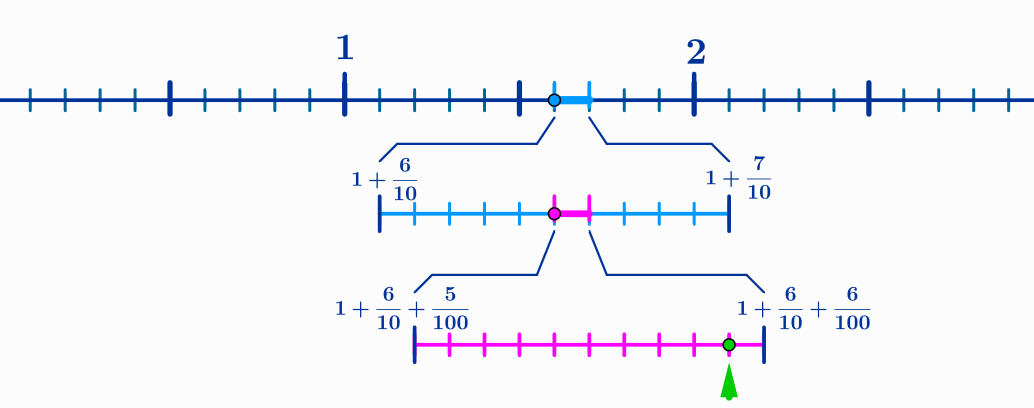
\includegraphics[width=\linewidth]{frac_decimales_demi-droite_zoom.PNG}
\end{center}
\end{Mt}

% \section{Les savoir-faire du parcours}

% \begin{CpsCol}
% \begin{itemize}
% \item Savoir écrire une fraction décimale.
% \item Savoir compléter une égalité de fractions décimales.
% \item Savoir comparer une fraction décimale à l'unité.
% \item Savoir décomposer une fraction décimale.
% \item Savoir encadrer une fraction décimale par deux entiers consécutifs.
% \item Savoir ajouter des fractions décimales.
% \item Savoir utiliser des fractions décimales.
% \item Savoir repérer une fraction décimale sur une demi-droite graduée.
% \item Savoir placer une fraction décimale sur une demi-droite graduée.
% \end{itemize}
% \end{CpsCol}

% \end{document}

\end{pageCours} 
\begin{pageAD} 
 

\Sf{Connaitre le vocabulaire des opérations}
 
  
\begin{ExoCad}{Communiquer.}{1234}{2}{0}{0}{0}{0}

 
\end{ExoCad}

\Sf{Connaitre les règles de priorités}

\begin{ExoCad}{Calculer.}{1234}{0}{0}{0}{0}{0}

 
 
\end{ExoCad}

\begin{ExoCad}{Calculer.}{1234}{0}{0}{0}{0}{0}

 
\end{ExoCad}


\Sf{Utiliser la distributivité}

\begin{ExoCad}{Représenter. Calculer.}{1234}{0}{0}{0}{0}{0}

 
 
\end{ExoCad}

\begin{ExoCad}{Calculer.}{1234}{0}{0}{0}{0}{0}

 
\end{ExoCad}

 
\end{pageAD}


%%%%%%%%%%%%%%%%%%%%%%%%%%%%%%%%%%%%%%%%%%%%%%%%%%%%%%%%%%%%%%%%%%%
%%%%  Niveau 1
%%%%%%%%%%%%%%%%%%%%%%%%%%%%%%%%%%%%%%%%%%%%%%%%%%%%%%%%%%%%%%%%%%%
\begin{pageParcoursu} 

 %%%%%%%%%%%%%%%%%%%%%%%%%%%
\begin{ExoCu}{Représenter.}{1234}{2}{0}{0}{0}{0}


\end{ExoCu}
%%%%%%%%%%%%%%%%%%%%%%%%%%%
\begin{ExoCu}{Représenter.}{1234}{2}{0}{0}{0}{0}


\end{ExoCu}
%%%%%%%%%%%%%%%%%%%%%%%%%%%
\begin{ExoCu}{Représenter.}{1234}{2}{0}{0}{0}{0}

\end{ExoCu}


%%%%%%%%%%%%%%%%%%%%%%%%%%%
\begin{ExoCu}{Raisonner.}{1234}{2}{0}{0}{0}{0}

\end{ExoCu}

%%%%%%%%%%%%%%%%%%%%%%%%%%%
\begin{ExoCu}{Représenter.}{1234}{2}{0}{0}{0}{0}


\end{ExoCu}


\end{pageParcoursu}

  
%%%%%%%%%%%%%%%%%%%%%%%%%%%%%%%%%%%%%%%%%%%%%%%%%%%%%%%%%%%%%%%%%%%
%%%%  Niveau 2
%%%%%%%%%%%%%%%%%%%%%%%%%%%%%%%%%%%%%%%%%%%%%%%%%%%%%%%%%%%%%%%%%%%



\begin{pageParcoursd} 
 
%%%%%%%%%%%%%%%%%%%%%%%%%%%%%%%%%%%%%%%%%%%%%%%%%%%%%%%%%%%%%%%%%%%
\begin{ExoCd}{Représenter.}{1234}{2}{0}{0}{0}{0}


 
\end{ExoCd}

 
%%%%%%%%%%%%%%%%%%%%%%%%%%%%%%%%%%%%%%%%%%%%%%%%%%%%%%%%%%%%%%%%%%%
\begin{ExoCd}{Chercher.communiquer.}{1234}{2}{0}{0}{0}{0}



\end{ExoCd}


%%%%%%%%%%%%%%%%%%%%%%%%%%%%%%%%%%%%%%%%%%%%%%%%%%%%%%%%%%%%%%%%%%%
\begin{ExoCd}{Représenter. Raisonner.}{1234}{2}{0}{0}{0}{0}


\end{ExoCd}

 %%%%%%%%%%%%%%%%%%%%%%%%%%%%%%%%%%%%%%%%%%%%%%%%%%%%%%%%%%%%%%%%%%%
\begin{ExoCd}{Représenter. Raisonner.}{1234}{2}{0}{0}{0}{0}


\end{ExoCd}
 
%%%%%%%%%%%%%%%%%%%%%%%%%%%%%%%%%%%%%%%%%%%%%%%%%%%%%%%%%%%%%%%%%%%
\begin{ExoCd}{Représenter. Raisonner.}{1234}{2}{0}{0}{0}{0}


\end{ExoCd}
 
\end{pageParcoursd}

%%%%%%%%%%%%%%%%%%%%%%%%%%%%%%%%%%%%%%%%%%%%%%%%%%%%%%%%%%%%%%%%%%%
%%%%  Niveau 3
%%%%%%%%%%%%%%%%%%%%%%%%%%%%%%%%%%%%%%%%%%%%%%%%%%%%%%%%%%%%%%%%%%%
\begin{pageParcourst}

%%%%%%%%%%%%%%%%%%%%%%%%%%%%%%%%%%%%%%%%%%%%%%%%%%%%%%%%%%%%%%%%%%%
\begin{ExoCt}{Représenter.}{1234}{2}{0}{0}{0}{0}

 

\end{ExoCt}

%%%%%%%%%%%%%%%%%%%%%%%%%%%%%%%%%%%%%%%%%%%%%%%%%%%%%%%%%%%%%%%%%%%
\begin{ExoCt}{Représenter. Raisonner.}{1234}{2}{0}{0}{0}{0}
 
 


\end{ExoCt}


%%%%%%%%%%%%%%%%%%%%%%%%%%%%%%%%%%%%%%%%%%%%%%%%%%%%%%%%%%%%%%%%%%%
\begin{ExoCt}{Raisonner.}{1234}{2}{0}{0}{0}{0}
 
\end{ExoCt}

%%%%%%%%%%%%%%%%%%%%%%%%%%%%%%%%%%%%%%%%%%%%%%%%%%%%%%%%%%%%%%%%%%%
\begin{ExoCt}{Représenter.}{1234}{2}{0}{0}{0}{0}

 

\end{ExoCt}

%%%%%%%%%%%%%%%%%%%%%%%%%%%%%%%%%%%%%%%%%%%%%%%%%%%%%%%%%%%%%%%%%%%
\begin{ExoCt}{Représenter.}{1234}{2}{0}{0}{0}{0}

 

\end{ExoCt} 
 
\end{pageParcourst}

%%%%%%%%%%%%%%%%%%%%%%%%%%%%%%%%%%%%%%%%%%%%%%%%%%%%%%%%%%%%%%%%%%%
%%%%  Brouillon
%%%%%%%%%%%%%%%%%%%%%%%%%%%%%%%%%%%%%%%%%%%%%%%%%%%%%%%%%%%%%%%%%%%


\begin{pageBrouillon} 
 
\ligne{32}



\end{pageBrouillon}

%%%%%%%%%%%%%%%%%%%%%%%%%%%%%%%%%%%%%%%%%%%%%%%%%%%%%%%%%%%%%%%%%%%
%%%%  Auto
%%%%%%%%%%%%%%%%%%%%%%%%%%%%%%%%%%%%%%%%%%%%%%%%%%%%%%%%%%%%%%%%%%%


%%%%%%%%%%%%%%%%%%%%%%%%%%%%%%%%%%%%%%%%%%%%%%%%%%%%%%%%%%%%%%%%%%%
\begin{pageAuto} 


\begin{ExoAuto}{Raisonner.}{1234}{2}{0}{0}{0}{0}

 
%%%%%%%%%%%%%%%%%%%%%%%%%%%%%%%%%%%%%%%%%%%%%%%%%%%%%%%%%%%%%%%%%%%
\end{ExoAuto}

\begin{ExoAuto}{Raisonner.}{1234}{2}{0}{0}{0}{0}
  

\end{ExoAuto}

%%%%%%%%%%%%%%%%%%%%%%%%%%%%%%%%%%%%%%%%%%%%%%%%%%%%%%%%%%%%%%%%%%%
\begin{ExoAuto}{Raisonner.}{1234}{2}{0}{0}{0}{0}

 
 

\end{ExoAuto}

 
%%%%%%%%%%%%%%%%%%%%%%%%%%%%%%%%%%%%%%%%%%%%%%%%%%%%%%%%%%%%%%%%%%%
\begin{ExoAuto}{Raisonner.}{1234}{2}{0}{0}{0}{0}

 
 

\end{ExoAuto}


\end{pageAuto}

%%%-----------
%%
%%% Les nombres entiers
%% \documentclass[a4paper,dvipsnames]{article}

% \addtolength{\hoffset}{-2.25cm}
% \addtolength{\textwidth}{4.5cm}
% \addtolength{\voffset}{-3.25cm}
% \addtolength{\textheight}{5cm}
% \setlength{\parskip}{0pt}
% \setlength{\parindent}{0in}

% %----------------------------------------------------------------------------------------
%	PACKAGES AND OTHER DOCUMENT CONFIGURATIONS
%----------------------------------------------------------------------------------------

%----------------------------------------------------------------------------------------
%		Generals
%----------------------------------------------------------------------------------------
\usepackage{fourier}
\usepackage{frcursive}
\usepackage[T1]{fontenc} %Accents handling
\usepackage[utf8]{inputenc} % Use UTF-8 encoding
%\usepackage{microtype} % Slightly tweak font spacing for aesthetics
\usepackage[english, francais]{babel} % Language hyphenation and typographical rules

%----------------------------------------------------------------------------------------
%		Graphics
%----------------------------------------------------------------------------------------
\usepackage{xcolor}
\usepackage{graphicx, multicol} % Enhanced support for graphics
\graphicspath{{FIG/}}
\usepackage{wrapfig}

%----------------------------------------------------------------------------------------
%		Other packages
%----------------------------------------------------------------------------------------
\usepackage{hyperref}
\hypersetup{
	colorlinks=true, %colorise les liens
	breaklinks=true, %permet le retour à la ligne dans les liens trop longs
	urlcolor= bleu3,  %couleur des hyperliens
	linkcolor= bleu3, %couleur des liens internes
	plainpages=false  %pour palier à "Bookmark problems can occur when you have duplicate page numbers, for example, if you have a page i and a page 1."
}
\usepackage{tabularx}
\newcolumntype{M}[1]{>{\arraybackslash}m{#1}} %Defines a scalable column type in tabular
\usepackage{booktabs} % Enhances quality of tables
\usepackage{diagbox} % barre en diagonale dans un tableau
\usepackage{multicol}
\usepackage[explicit]{titlesec}


%----------------------------------------------------------------------------------------
%		Headers and footers
%----------------------------------------------------------------------------------------
\usepackage{fancyhdr} % Headers and footers
\pagestyle{fancy} % All pages have headers and footers
\fancyhead{}\renewcommand{\headrulewidth}{0pt} % Blank out the default header
\renewcommand{\footrulewidth}{0pt}
\fancyfoot[L]{} % Custom footer text
\fancyfoot[C]{\href{https://sacado.xyz/}{sacado.xyz}} % Custom footer text
\fancyfoot[R]{\thepage} % Custom footer text

%----------------------------------------------------------------------------------------
%		Mathematics packages
%----------------------------------------------------------------------------------------
\usepackage{amsthm, amsmath, amssymb} % Mathematical typesetting
\usepackage{marvosym, wasysym} % More symbols
\usepackage[makeroom]{cancel}
\usepackage{xlop}
\usepackage{pgf,tikz,pgfplots}
\pgfplotsset{compat=1.15}
\usetikzlibrary{positioning}
%\usetikzlibrary{arrows}
\usepackage{pst-plot,pst-tree,pst-func, pstricks-add,pst-node,pst-text}
\usepackage{units}
\usepackage{nicefrac}
\usepackage[np]{numprint} %Séparation milliers dans un nombre

%----------------------------------------------------------------------------------------
%		New text commands
%----------------------------------------------------------------------------------------
\usepackage{calc}
\usepackage{boites}
 \renewcommand{\arraystretch}{1.6}

%%%%% Pour les imports.
\usepackage{import}

%%%%% Pour faire des boites
\usepackage[tikz]{bclogo}
\usepackage{bclogo}
\usepackage{framed}
\usepackage[skins]{tcolorbox}
\tcbuselibrary{breakable}
\tcbuselibrary{skins}
\usetikzlibrary{babel,arrows,shadows,decorations.pathmorphing,decorations.markings,patterns}

%%%%% Pour les symboles et les ensembles
\newcommand{\pp}{\leq}
\newcommand{\pg}{\geq}
%\newcommand{\euro}{\eurologo{}}
\newcommand{\R}{\mathbb{R}}
\newcommand{\N}{\mathbb{N}}
\newcommand{\D}{\mathbb{D}}
\newcommand{\Z}{\mathbb{Z}}
\newcommand{\Q}{\mathbb{Q}}
\newcommand{\C}{\mathbb{C}}

%%%%% Pour une double minipage
\newcommand{\mini}[2]{
\begin{minipage}[t]{0.48\linewidth}
#1
\end{minipage}
\hfill
\begin{minipage}[t]{0.48\linewidth}
#2
\end{minipage}
}


%\newcommand\hole[1]{\texttt{\_}}
%\newcommand{\PROP}[1]{\textbf{\underline{#1}}}
%\newcommand{\exercice}{\textcolor{OliveGreen}{Exercice : }}
%\newcommand{\correction}{\textcolor{BurntOrange}{Correction : }}
%\newcommand{\propriete}{\textbf{\underline{Propriété}} : }
%\newcommand{\prop}{\textbf{\underline{Propriété}} : }
%\newcommand{\vocabulaire}{\textbf{\underline{Vocabulaire}} : }
%\newcommand{\voca}{\textbf{\underline{Vocabulaire}} : }

\usepackage{enumitem}
\newlist{todolist}{itemize}{2} %Pour faire des QCM
\setlist[todolist]{label=$\square$} %Pour faire des QCM \begin{todolist} instead of itemize

%----------------------------------------------------------------------------------------
%		Définition de couleur pour geogebra
%----------------------------------------------------------------------------------------
\definecolor{zzttqq}{rgb}{0.6,0.2,0.} %rouge des polygones
\definecolor{qqqqff}{rgb}{0.,0.,1.}
\definecolor{xdxdff}{rgb}{0.49019607843137253,0.49019607843137253,1.}%bleu
\definecolor{qqwuqq}{rgb}{0.,0.39215686274509803,0.} %vert des angles
\definecolor{ffqqqq}{rgb}{1.,0.,0.} %rouge vif
\definecolor{uuuuuu}{rgb}{0.26666666666666666,0.26666666666666666,0.26666666666666666}
\definecolor{qqzzqq}{rgb}{0.,0.6,0.}
\definecolor{cqcqcq}{rgb}{0.7529411764705882,0.7529411764705882,0.7529411764705882} %gris
\definecolor{qqffqq}{rgb}{0.,1.,0.}
\definecolor{ffdxqq}{rgb}{1.,0.8431372549019608,0.}
\definecolor{ffffff}{rgb}{1.,1.,1.}
\definecolor{ududff}{rgb}{0.30196078431372547,0.30196078431372547,1.}

%-------------------------------------------------
%
%	EN TETE
%
%-------------------------------------------------

% Classe
\newcommand{\myClasse}   
{
    6e
}

% Discipline
\newcommand{\myDiscipline}   
{
    Mathématiques
}

% Parcours
\newcommand{\myParcours}
{
  Nombres et Calculs
}

%Titre de la séquence
\newcommand{\myTitle}
{
    \scshape\huge
\textcolor{sacado_purple}{
		Nombres décimaux
}
}

%----------------------------------------------------------------------------------------

% %----------------------------------------------------------------------------------------
%		Définition de couleur pour les boites
%----------------------------------------------------------------------------------------
\definecolor{bleu1}{rgb}{0.54,0.79,0.95} %% Bleu
\definecolor{sapgreen}{rgb}{0.4, 0.49, 0}
\definecolor{dvzfxr}{rgb}{0.7,0.4,0.}
\definecolor{beamer}{rgb}{0.5176470588235295,0.49019607843137253,0.32941176470588235} % couleur beamer
\definecolor{preuveRbeamer}{rgb}{0.8,0.4,0}
\definecolor{sectioncolor}{rgb}{0.24,0.21,0.44}
\definecolor{subsectioncolor}{rgb}{0.1,0.21,0.61}
\definecolor{subsubsectioncolor}{rgb}{0.1,0.21,0.61}
\definecolor{info}{rgb}{0.82,0.62,0}
\definecolor{bleu2}{rgb}{0.38,0.56,0.68}
\definecolor{bleu3}{rgb}{0.24,0.34,0.40}
\definecolor{bleu4}{rgb}{0.12,0.20,0.25}
\definecolor{vert}{rgb}{0.21,0.33,0}
\definecolor{vertS}{rgb}{0.05,0.6,0.42}
\definecolor{red}{rgb}{0.78,0,0}
\definecolor{color5}{rgb}{0,0.4,0.58}
\definecolor{eduscol4B}{rgb}{0.19,0.53,0.64}
\definecolor{eduscol4P}{rgb}{0.62,0.12,0.39}

%----------------------------------------------------------------------------------------
%		Définition de couleur pour les boites SACADO
%----------------------------------------------------------------------------------------
\definecolor{sacado_blue}{RGB}{0,129,159} %% Bleu Sacado
\definecolor{sacado_green}{RGB}{59, 157, 38} %% Vert Sacado
\definecolor{sacado_yellow}{RGB}{255,180,0} %% Jaune Sacado
\definecolor{sacado_purple}{RGB}{94,68,145} %% Violet foncé Sacado
\definecolor{sacado_violet}{RGB}{153,117,224} %% Violet clair Sacado
\definecolor{sacado_orange}{RGB}{249,168,100} %% Orange Sacado
\definecolor{ill_frame}{HTML}{F0F0F0}
\definecolor{ill_back}{HTML}{F7F7F7}
\definecolor{ill_title}{HTML}{AAAAAA}


 % Compteurs pour Théorème, Définition, Exemple, Remarque, .....
\newcounter{cpttheo}
\setcounter{cpttheo}{0}
\newcounter{cptdef}
\setcounter{cptdef}{0}
\newcounter{cptmth}
\setcounter{cptmth}{0}
\newcounter{cpttitre}
\setcounter{cpttitre}{0}
 % Exercices
\newcounter{cptapp}
\setcounter{cptapp}{0}
\newcounter{cptex}
\setcounter{cptex}{0}
\newcounter{cptsr}
\setcounter{cptsr}{0}
\newcounter{cpti}
\setcounter{cpti}{0}
\newcounter{cptcor}
\setcounter{cptcor}{0}




%%%%% Pour réinitialiser numéros des paragraphes après une nouvelle partie
\makeatletter
    \@addtoreset{paragraph}{part}
\makeatother


%%%% Titres et sections

\newlength\chapnumb
\setlength\chapnumb{3cm}


% \titleformat{\part}[block] {
 % \normalfont\sffamily\color{violet}}{}{0pt} {
   % \parbox[t]{\chapnumb}{\fontsize{120}{110}\selectfont\ding{110}}
   % \parbox[b]{\dimexpr\textwidth-\chapnumb\relax}{
       % \raggedleft
       % \hfill{{\color{bleu3}\fontsize{40}{30}\selectfont#1}}\\
       % \rule{0.99\textwidth-\chapnumb\relax}{0.4pt}
 % }
% }

% \titleformat{name=\part,numberless}[block]
% {\normalfont\sffamily\color{bleu3}}{}{0pt}
% {\parbox[b]{\chapnumb}{%
  % \mbox{}}%
 % \parbox[b]{\dimexpr\textwidth-\chapnumb\relax}{%
   % \raggedleft%
   % \hfill{{\color{bleu3}\fontsize{40}{30}\selectfont#1}}\\
   % \rule{0.99\textwidth-\chapnumb\relax}{0.4pt}
 % }
% }



% \titleformat{\chapter}[block] {
 % \normalfont\sffamily\color{violet}}{}{0pt} {
   % \parbox[t]{\chapnumb}{ 
     % \fontsize{120}{110}\selectfont\thechapter}
     % \parbox[b]{\textwidth-\chapnumb}{
       % \raggedleft
       % \hfill{{\color{bleu3}\huge#1}}\\  
  % \ifthenelse{\thechapter<10}{\rule{0.99\textwidth-\chapnumb}{0.4pt}}{\rule{0.9\textwidth - \chapnumb}{0.4pt}}
       % \setcounter{cpttitre}{0}
	% \setcounter{cptapp}{0}
	% \setcounter{cptex}{0}
	% \setcounter{cptsr}{0}
	% \setcounter{cpti}{0}
	% \setcounter{cptcor}{0} 
 % }
% }

% \titleformat{name=\chapter,numberless}[block]
% {\normalfont\sffamily\color{bleu3}}{}{0pt}
% {\parbox[b]{\chapnumb}{%
  % \mbox{}}%
 % \parbox[b]{\textwidth-\chapnumb}{%
   % \raggedleft
   % \hfill{{\color{bleu3}\huge#1}}\\
   % \ifthenelse{\thechapter<10}{\rule{0.99\textwidth-\chapnumb}{0.4pt}}{ \rule{0.9\textwidth - \chapnumb}{0.4pt}}
       % \setcounter{cpttitre}{0}
	% \setcounter{cptapp}{0}
	% \setcounter{cptex}{0}
	% \setcounter{cptsr}{0}
	% \setcounter{cpti}{0}
	% \setcounter{cptcor}{0} 
 % }
% }
%
%       
%
%%%%% Personnalisation des numéros des sections
\renewcommand\thesection{\Roman{section}. }
\renewcommand\thesubsection{\hspace{1cm}\arabic{subsection}. }
\renewcommand\thesubsubsection{\hspace{2cm}\alph{subsubsection}. }

\titleformat{\section}[hang]{\color{sacado_purple}{}\normalfont\filright\huge}{}{0.4em}{\textbf{\thesection  #1}}   
% \titlespacing*{\section}{0.2pt}{0ex plus 0ex minus 0ex}{0.3em}
   
\titleformat{\subsection}[hang]{\color{sacado_purple}{}\normalfont\filright\Large}{}{0.4em}{\thesubsection
 #1}            
\titleformat{\subsubsection}[hang]{\color{sacado_purple}{}\normalfont\filright\large}{}{0.4em}{\thesubsubsection
 #1}
\titleformat{\paragraph}[hang]{\color{black}{}\normalfont\filright\normalsize}{}{0.4em}{#1}



%%%%%%%%%%%%%%%%%%%%% Cycle 4
%\newcommand{\Titre}[2]{\section*{#1 
%\ifthenelse{\equal{#2}{1}}   {\hfill{ \ding{182}  \ding{173} \ding{174} } \addcontentsline{toc}{section}{#1 \ding{182}} }%
%{%
%\ifthenelse{\equal{#2}{2}}{\hfill{ \ding{172}  \ding{183} \ding{174} } \addcontentsline{toc}{section}{#1 {\color{purple}\ding{183}}} }{%           
%\hfill{ \ding{172}  \ding{173} \ding{184} } \addcontentsline{toc}{section}{#1 {\color{orange}\ding{184}}}% 
%}%
%}%
%}
%}


%%%%%%%%%%%%%%%%%%%%% Cycle 4
\newcommand{\Titre}[2]{\section*{#1 
\ifthenelse{\equal{#2}{1}}   {\hfill{ \ding{182}  \ding{173} \ding{174} } \addcontentsline{toc}{section}{#1 \, \ding{182}} }%
{% sinon
\ifthenelse{\equal{#2}{1,5}}   {\hfill{ \ding{182}  \ding{183} \ding{174} } \addcontentsline{toc}{section}{#1 \, \ding{182} {\color{purple}\ding{183}}} }%
{% sinon
\ifthenelse{\equal{#2}{2}}   {\hfill{ \ding{172}  \ding{183} \ding{174} } \addcontentsline{toc}{section}{#1 \, {\color{purple}\ding{183}}} }
{% sinon
\ifthenelse{\equal{#2}{2,5}}   {\hfill{ \ding{172}  \ding{183} \ding{184} } \addcontentsline{toc}{section}{#1 \, {\color{purple}\ding{183}}  {\color{orange}\ding{184}}} }%
{% sinon
\hfill{ \ding{172}  \ding{173} \ding{184} } \addcontentsline{toc}{section}{#1 \,{\color{orange}\ding{184}}}% 
}%
}%
}%
}%
}%
}

%%%%%%%%%%%%% Titre
\newenvironment{titre}[2][]{%
\vspace{0.5cm}
\begin{tcolorbox}[enhanced, lifted shadow={0mm}{0mm}{0mm}{0mm}%
{black!60!white}, attach boxed title to top left={xshift=110mm, yshift*=-3mm}, coltitle=violet, colback=bleu3!25!white, boxed title style={colback=white!100}, colframe=bleu3,title=\stepcounter{cpttitre} \textbf{Fiche \thecpttitre}. #1 #2 ]}
{%
\end{tcolorbox}
\par}



%%%%%%%%%%%%% Définitions
\newenvironment{Def}[1][]{%
\medskip \begin{tcolorbox}[widget,colback=sacado_violet!0,colframe=sacado_violet!75,
adjusted title= \stepcounter{cptdef} Définition \thecptdef . {#1} ]}
{%
\end{tcolorbox}\par}


\newenvironment{DefT}[2][]{%
\medskip \begin{tcolorbox}[widget,colback=sacado_violet!0,colframe=sacado_violet!75,
adjusted title= \stepcounter{cptdef} Définition \thecptdef . {#1} \textit{#2}]}
{%
\end{tcolorbox}\par}

%%%%%%%%%%%%% Proposition
\newenvironment{Prop}[1][]{%
\medskip \begin{tcolorbox}[widget,colback=sacado_blue!0,colframe=sacado_blue!75!black,
adjusted title= \stepcounter{cpttheo} Proposition \thecpttheo . {#1} ]}
{%
\end{tcolorbox}\par}

%%%%%%%%%%%%% Propriétés
\newenvironment{Pp}[1][]{%
\medskip \begin{tcolorbox}[widget,colback=sacado_blue!0,colframe=sacado_blue!75!black,
adjusted title= \stepcounter{cpttheo} Propriété \thecpttheo . {#1}]}
{%
\end{tcolorbox}\par}

\newenvironment{PpT}[2][]{%
\medskip \begin{tcolorbox}[widget,colback=sacado_blue!0,colframe=sacado_blue!75!black,
adjusted title= \stepcounter{cpttheo} Propriété \thecpttheo . {#1} #2]}
{%
\end{tcolorbox}\par}

\newenvironment{Pps}[1][]{%
\medskip \begin{tcolorbox}[widget,colback=sacado_blue!0,colframe=sacado_blue!75!black,
adjusted title= \stepcounter{cpttheo} Propriétés \thecpttheo . {#1}]}
{%
\end{tcolorbox}\par}

%%%%%%%%%%%%% Théorèmes
\newenvironment{ThT}[2][]{% théorème avec titre
\medskip \begin{tcolorbox}[widget,colback=sacado_blue!0,colframe=sacado_blue!75!black,
adjusted title= \stepcounter{cpttheo} Théorème \thecpttheo . {#1} #2]}
{%
\end{tcolorbox}\par}

\newenvironment{Th}[1][]{%
\medskip \begin{tcolorbox}[widget,colback=sacado_blue!0,colframe=sacado_blue!75!black,
adjusted title= \stepcounter{cpttheo} Théorème \thecpttheo . {#1}]}
{%
\end{tcolorbox}\par}

%%%%%%%%%%%%% Règles
\newenvironment{Reg}[1][]{%
\medskip \begin{tcolorbox}[widget,colback=sacado_blue!0,colframe=sacado_blue!75!black,
adjusted title= \stepcounter{cpttheo} Règle \thecpttheo . {#1}]}
{%
\end{tcolorbox}\par}

%%%%%%%%%%%%% REMARQUES
\newenvironment{Rq}[1][]{%
\begin{bclogo}[couleur=sacado_orange!0, arrondi =0.15, noborder=true, couleurBarre=sacado_orange, logo = \bcinfo ]{ 
{\color{info}\normalsize{Remarque#1}}}}
{%
\end{bclogo}
\par}


\newenvironment{Rqs}[1][]{%
\begin{bclogo}[couleur=sacado_orange!0, arrondi =0.15, noborder=true, couleurBarre=sacado_orange, logo = \bcinfo ]{ 
{\color{info}\normalsize{Remarques#1}}}}
{%
\end{bclogo}
\par}

%%%%%%%%%%%%% EXEMPLES
\newenvironment{Ex}[1][]{%
\begin{bclogo}[couleur=sacado_yellow!15, arrondi =0.15, noborder=true, couleurBarre=sacado_yellow, logo = \bclampe ]{ 
\normalsize{Exemple#1}}}
{%
\end{bclogo}
\par}




%%%%%%%%%%%%% Preuve
\newenvironment{Pv}[1][]{%
\begin{tcolorbox}[breakable, enhanced,widget, colback=sacado_blue!10!white,boxrule=0pt,frame hidden,
borderline west={1mm}{0mm}{sacado_blue!75}]
\textbf{Preuve#1 : }}
{%
\end{tcolorbox}
\par}


%%%%%%%%%%%%% PreuveROC
\newenvironment{PvR}[1][]{%
\begin{tcolorbox}[breakable, enhanced,widget, colback=sacado_blue!10!white,boxrule=0pt,frame hidden,
borderline west={1mm}{0mm}{sacado_blue!75}]
\textbf{Preuve (ROC)#1 : }}
{%
\end{tcolorbox}
\par}


%%%%%%%%%%%%% Compétences
\newenvironment{Cps}[1][]{%
\vspace{0.4cm}
\begin{tcolorbox}[enhanced, lifted shadow={0mm}{0mm}{0mm}{0mm}%
{black!60!white}, attach boxed title to top left={xshift=5mm, yshift*=-3mm}, coltitle=white, colback=white, boxed title style={colback=sacado_green!100}, colframe=sacado_green!75!black,title=\textbf{Compétences associées#1}]}
{%
\end{tcolorbox}
\par}

%%%%%%%%%%%%% Compétences Collège
\newenvironment{CpsCol}[1][]{%
\vspace{0.4cm}
\begin{tcolorbox}[breakable, enhanced,widget, colback=white ,boxrule=0pt,frame hidden,
borderline west={2mm}{0mm}{bleu3}]
\textbf{#1}}
{%
\end{tcolorbox}
\par}




%%%%%%%%%%%%% Attendus
\newenvironment{Ats}[1][]{%
\vspace{0.4cm}
\begin{tcolorbox}[enhanced, lifted shadow={0mm}{0mm}{0mm}{0mm}%
{black!60!white}, attach boxed title to top left={xshift=5mm, yshift*=-3mm}, coltitle=white, colback=white, boxed title style={colback=sacado_green!100}, colframe=sacado_green!75!black,title=\textbf{Attendus du chapitre#1}]}
{%
\end{tcolorbox}
\par}

%%%%%%%%%%%%% Méthode
\newenvironment{Mt}[1][]{%
\vspace{0.4cm}
\begin{bclogo}[couleur=sacado_blue!0, arrondi =0.15, noborder=true, couleurBarre=bleu3, logo = \bccrayon ]{ 
\normalsize{{\color{bleu3}Méthode #1}}}}
{%
\end{bclogo}
\par}


%%%%%%%%%%%%% Méthode en vidéo
\newcommand{\MtV}[2]{\vspace{0.4cm} \colorbox{sacado_blue!0}{\hspace{0.2 cm}\tikz\node[rounded corners=1pt,draw] {\color{red}$\blacktriangleright$}; \quad  \href{https://youtu.be/#1?rel=0}{\raisebox{0.8mm}{{\color{red}\textbf{Méthode en vidéo : #2}}}}}}


%%%%%%%%%%%%% A voir (AV) : Lien externe + vidéo non Youtube
\newcommand{\AV}[2]{\vspace{0.4cm} \colorbox{bleu1!0}{\hspace{0.2 cm}\tikz\node[rounded corners=1pt,draw] {\color{red}$\blacktriangleright$}; \quad  \href{#1}{\raisebox{0.8mm}{{\color{red}\textbf{#2}}}}}}


%%%%%%%%%%%%% Etymologie
\newenvironment{Ety}[1][]{%
\begin{bclogo}[couleur=sacado_green!0, arrondi =0.15, noborder=true, couleurBarre=sacado_green, logo = \bcplume ]{ 
\normalsize{{\color{sacado_green}Étymologie#1}}}}
{%
\end{bclogo}
\par}


%%%%%%%%%%%%% Notation
\newenvironment{Nt}[1][]{%
\begin{bclogo}[couleur=sacado_violet!0, arrondi =0.15, noborder=true, couleurBarre=sacado_violet!75, logo = \bccrayon ]{ 
\normalsize{{\color{violet!75}Notation#1}}}}
{%
\end{bclogo}
\par}
%%%%%%%%%%%%% Histoire
%\newenvironment{His}[1][]{%
%\begin{bclogo}[couleur=brown!30, arrondi =0.15, noborder=true, couleurBarre=brown, logo = \bcvaletcoeur ]{ 
%\normalsize{{\color{brown}Histoire des mathématiques#1}}}}
%{%
%\end{bclogo}
%\par}

\newenvironment{His}[1][]{%
\vspace{0.4cm}
\begin{tcolorbox}[enhanced, lifted shadow={0mm}{0mm}{0mm}{0mm}%
{brown!60!white}, attach boxed title to top left={xshift=5mm, yshift*=-3mm}, coltitle=white, colback=white, boxed title style={colback=brown!100}, colframe=brown!75!black,title=\textbf{Histoire des mathématiques#1}]}
{%
\end{tcolorbox}
\par}

%%%%%%%%%%%%% Attention
\newenvironment{Att}[1][]{%
\begin{bclogo}[couleur=red!0, arrondi =0.15, noborder=true, couleurBarre=red, logo = \bcattention ]{ 
\normalsize{{\color{red}Attention. #1}}}}
{%
\end{bclogo}
\par}


%%%%%%%%%%%%% Conséquence
\newenvironment{Cq}[1][]{%
\textbf{Conséquence #1}}
{%
\par}

%%%%%%%%%%%%% Vocabulaire
\newenvironment{Voc}[1][]{%
\setlength{\logowidth}{10pt}
%\begin{footnotesize}
\begin{bclogo}[ noborder , couleur=white, logo =\bcbook]{#1}}
{%
\end{bclogo}
%\end{footnotesize}
\par}


%%%%%%%%%%%%% Video
\newenvironment{Vid}[1][]{%
\setlength{\logowidth}{12pt}
\begin{bclogo}[ noborder , couleur=white,barre=none, logo =\bcoeil]{#1}}
{%
\end{bclogo}
\par}


%%%%%%%%%%%%% Syntaxe
\newenvironment{Syn}[1][]{%
\begin{bclogo}[couleur=violet!0, arrondi =0.15, noborder=true, couleurBarre=violet!75, logo = \bcicosaedre ]{ 
\normalsize{{\color{violet!75}Syntaxe#1}}}}
{%
\end{bclogo}
\par}

%%%%%%%%%%%%% Auto évaluation
\newenvironment{autoeval}[1][]{%
\vspace{0.4cm}
\begin{tcolorbox}[enhanced, lifted shadow={0mm}{0mm}{0mm}{0mm}%
{black!60!white}, attach boxed title to top left={xshift=5mm, yshift*=-3mm}, coltitle=white, colback=white, boxed title style={colback=sacado_green!100}, colframe=sacado_green!75!black,title=\textbf{J'évalue mes compétences#1}]}
{%
\end{tcolorbox}
\par}


\newenvironment{autotest}[1][]{%
\vspace{0.4cm}
\begin{tcolorbox}[enhanced, lifted shadow={0mm}{0mm}{0mm}{0mm}%
{red!60!white}, attach boxed title to top left={xshift=5mm, yshift*=-3mm}, coltitle=white, colback=white, boxed title style={colback=red!100}, colframe=red!75!black,title=\textbf{Pour faire le point #1}]}
{%
\end{tcolorbox}
\par}

\newenvironment{ExOApp}[1][]{% Exercice d'application direct
\vspace{0.4cm}
\begin{tcolorbox}[enhanced, lifted shadow={0mm}{0mm}{0mm}{0mm}%
{red!60!white}, attach boxed title to top left={xshift=5mm, yshift*=-3mm}, coltitle=white, colback=white, boxed title style={colback=sacado_green!100}, colframe=sacado_green!75!black,title=\textbf{Application #1}]}
{%
\end{tcolorbox}
\par}

\newenvironment{ExOInt}[1][]{% Exercice d'application direct
\vspace{0.4cm}
\begin{tcolorbox}[enhanced, lifted shadow={0mm}{0mm}{0mm}{0mm}%
{red!60!white}, attach boxed title to top left={xshift=5mm, yshift*=-3mm}, coltitle=white, colback=white, boxed title style={colback=sacado_green!50}, colframe=sacado_green!75!black,title=\textbf{Exercice #1}]}
{%
\end{tcolorbox}
\par}

%Illustrations
\newtcolorbox{Illqr}[1]{
  enhanced,
  colback=white,
  colframe=ill_frame,
  colbacktitle=ill_back,
  coltitle=ill_title,
  title=\textbf{Illustration},
  boxrule=1pt, % épaisseur du trait à 1pt
  center,
  overlay={
    \node[anchor=south east, inner sep=0pt,xshift=-1pt,yshift=2pt,fill=white] at (frame.south east) {\fancyqr[height=1cm]{#1}};
  },
  after=\par,
  before=\vspace{0.4cm},
}

\newtcolorbox{Ill}{
  enhanced,
  colback=white,
  colframe=ill_frame,
  colbacktitle=ill_back,
  coltitle=ill_title,
  title=\textbf{Illustration},
  boxrule=1pt, % épaisseur du trait à 1pt
  center,
  after=\par,
  before=\vspace{0.4cm},
}

%%%%%%%%%%%%%% Propriétés
%\newenvironment{Pp}[1][]{%
%\medskip \begin{tcolorbox}[widget,colback=sacado_blue!0,colframe=sacado_blue!75!black,
%adjusted title= \stepcounter{cpttheo} Propriété \thecpttheo . {#1}]}
%{%
%\end{tcolorbox}\par}

%%%%% Pour réinitialiser numéros des chapitres après une nouvelle partie
% \makeatletter
    % \@addtoreset{section}{part}
% \makeatother

% \newcommand{\EPC}[3]{ % Exercice par compétence de niveau 1
% \ifthenelse{\equal{#1}{1}}
% {%condition2 vraie
% \vspace{0.4cm}
% \stepcounter{cptex}
% \tikz\node[rounded corners=0pt,draw,fill=bleu2]{\color{white}\textbf{ \thecptex}}; \quad  {\color{bleu2}\textbf{#3}}
% \input{#2}
% }% fin condition2 vraie
% {%condition2 fausse
% \vspace{0.4cm}
% \stepcounter{cptex}
% \tikz\node[rounded corners=2pt,draw,fill=eduscol4P]{\color{white}\textbf{ \thecptex}}; \quad  {\color{eduscol4P} \textbf{En temps libre.} \textbf{ #3}} 
% \input{#2}
% }% fin condition2 fausse
% } % fin de la procédure

% \usepackage{hyperref}
% \usepackage{multido}
% \newcommand{\RNum}[1]{\uppercase\expandafter{\romannumeral #1\relax}}

% \begin{document}

%-------------------------------
%	TITLE SECTION
%-------------------------------

% \fancyhead[C]{}
% \hrule\medskip % Upper rule
% \begin{minipage}{0.295\textwidth} 
% \raggedright
% Classe \myClasse \hfill\\
% \myDiscipline \hfill\\
% \myParcours \hfill\\
% \end{minipage}
% \begin{minipage}{0.4\textwidth} 
% \centering 
% \scshape\huge
% \textcolor{sacado_purple}{\myTitle} \\ 
% \normalsize 
%%\mySubTitle \\ 
% \end{minipage}
% \begin{minipage}{0.295\textwidth} 
% \raggedleft
% \href{https://sacado.xyz/}{
\includegraphics[width=.2\linewidth]{sacadoA1.png}}
%%\myAnnee \hfill\\
% \end{minipage}
% \medskip \hrule
% \bigskip

%-------------------------------
%	CONTENTS
%-------------------------------

\chapter{Les nombres entiers}
{https://sacado.xyz/qcm/parcours_show_course/0/117118}

\begin{pageCours} 

\section{Un peu d'histoire de la numération}

\subsection{La numération Babylonienne}

\begin{His}
Vers le \RNum{2}e millénaire avant J.C., les babyloniens écrivent les nombres avec seulement deux symboles :\\
\begin{center}
\begin{tabular}{c|c|c}
Nom & Le "Clou vertical" & Le "Chevron" \\\hline
Symbole & 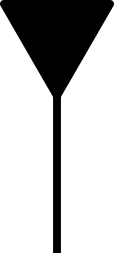
\includegraphics[width=.6cm]{clou_droit.png} & 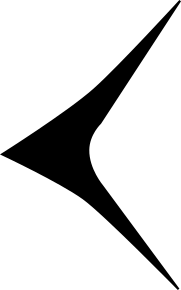
\includegraphics[width=.95cm]{chevron.png} \\\hline
Valeur & 1 & 10 \\
\end{tabular}
\end{center}

Ils utilisent un système sexagésimale (base $60$) et une numération de position. Suivant la place qu'occupe le symbole, celui-ci correspond soit à une unité, soit à une soixantaine ($60$), soit à une soixantaine de soixantaines ($60\times60=3\,600$). On utilise encore aujourd'hui un système sexagésimale pour les unités de temps et des mesures d'angles.\\

Exemples :
\begin{center}
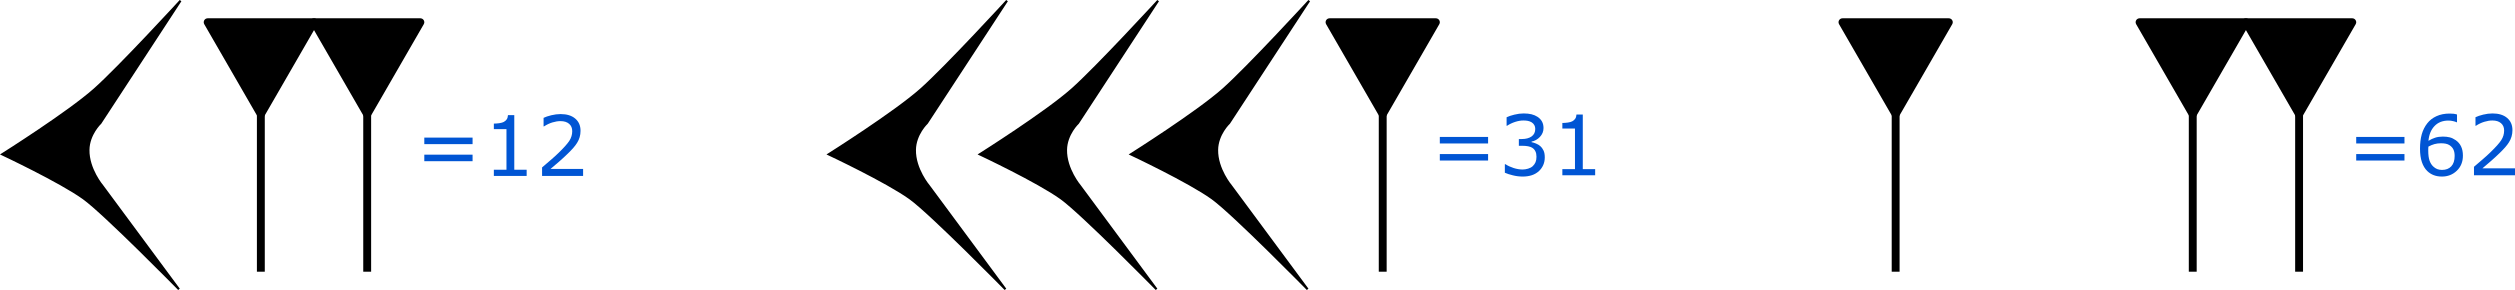
\includegraphics[width=9cm]{exemple_babylonian.png}
\end{center}
\end{His}

\subsection{La numération Égyptienne}

\begin{His}
Au \RNum{3}e millénaire avant J.C., en Egypte, les scribes écrivent les nombres sur des papyrus sous forme de hiéroglyphes. Les égyptiens utilisent un système de numération basé sur le principe additif. Les égyptiens peuvent écrire des nombres entiers jusqu'à $1\,000\,000$. Ils écrivent aussi des nombres décimaux et des fractions.

\newcommand{\egmil}[1]{\multido{\i=1+1}{#1}{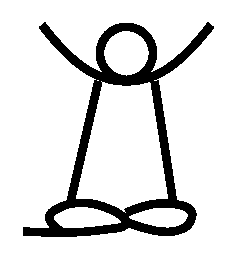
\includegraphics[scale=.1]{egyptian/egypt_person.eps}\hspace{0.5mm}}}
\newcommand{\eghuntho}[1]{\multido{\i=1+1}{#1}{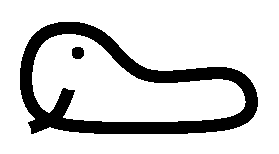
\includegraphics[scale=.1]{egyptian/egypt_fish.eps}\hspace{0.5mm}}}
\newcommand{\egtentho}[1]{\multido{\i=1+1}{#1}{
\includegraphics[scale=.1]{egyptian/egypt_finger.eps}\hspace{0.5mm}}}
\newcommand{\egtho}[1]{\multido{\i=1+1}{#1}{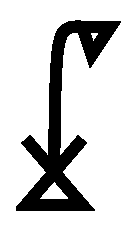
\includegraphics[scale=.1]{egyptian/egypt_lotus.eps}\hspace{0.5mm}}}
\newcommand{\eghun}[1]{\multido{\i=1+1}{#1}{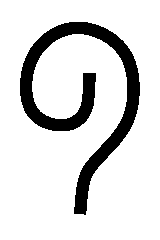
\includegraphics[scale=.1]{egyptian/egypt_scroll.eps}\hspace{0.5mm}}}
\newcommand{\egten}[1]{\multido{\i=1+1}{#1}{
\includegraphics[scale=.1]{egyptian/egypt_heel.eps}\hspace{0.5mm}}}
\newcommand{\egone}[1]{\multido{\i=1+1}{#1}{
\includegraphics[scale=.1]{egyptian/egypt_stroke.eps}\hspace{0.5mm}}}
\newcommand{\egyptify}[7]{
 \multido{\i=1+1}{#1}{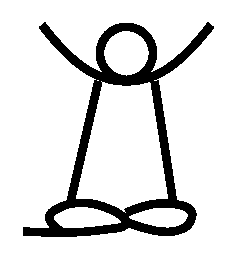
\includegraphics[scale=.1]{egyptian/egypt_person.eps}\hspace{0.5mm}}
 \multido{\i=1+1}{#2}{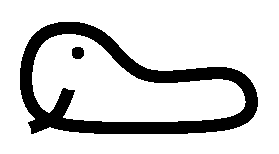
\includegraphics[scale=.1]{egyptian/egypt_fish.eps}\hspace{0.5mm}}
 \multido{\i=1+1}{#3}{
\includegraphics[scale=.1]{egyptian/egypt_finger.eps}\hspace{0.5mm}}
 \multido{\i=1+1}{#4}{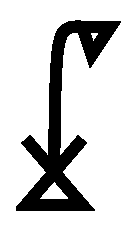
\includegraphics[scale=.1]{egyptian/egypt_lotus.eps}\hspace{0.5mm}}
 \multido{\i=1+1}{#5}{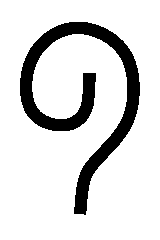
\includegraphics[scale=.1]{egyptian/egypt_scroll.eps}\hspace{0.5mm}}
 \multido{\i=1+1}{#6}{
\includegraphics[scale=.1]{egyptian/egypt_heel.eps}\hspace{0.5mm}}
 \multido{\i=1+1}{#7}{
\includegraphics[scale=.1]{egyptian/egypt_stroke.eps}\hspace{0.5mm}}
 \hspace{.5mm}
}

\begin{center}
\begin{tabular}[t]{c|c|c|c|c|c|c}
\egmil{1}&\eghuntho{1}&\egtentho{1}&\egtho{1}&\eghun{1}&\egten{1}&\egone{1}\\
\hline
1,000,000&100,000&10,000&1,000&100&10&1\\
\end{tabular}\\
\end{center}

Exemple :

\begin{center}
\egyptify{5}{8}{6}{7}{9}{3}{4}$=5\,867\,934$
\end{center}
\end{His}

\subsection{La numération Maya}

\begin{His}
Dans leur étude des astres, les mayas se servent des nombres pour calculer le temps. Ce sont les inventeurs du calendrier.

 Leur système de numération datant du \RNum{5}e siècle après J.C. suit le principe de position dans la base vigésimale (base $20$). Celui-ci trouve ses origines avec nos $10$ doigts et $10$ orteils !  
 
 Les symboles employés (les glyphes) représentent les nombres jusqu'à $19$, empilés sur différents niveaux. Chaque niveau correspond à un nombre de paquets de $20$ puis de $20\times20=400$ puis de $20\times20\times20=8\,000$...
 
Les mayas utilisent le zéro qu'ils représentent par un coquillage.

\begin{center}
\includegraphics[width=8cm]{maya_numerals.png}
\end{center}

Exemple : $379=18\times20+19$
\begin{center}
\includegraphics[width=1cm]{maya_exemple.png}
\end{center}
\end{His}

\subsection{La numération Romaine}

\begin{His}
Les grecs et les romains ont inventé des systèmes de numération alphabétiques très peu adaptés aux calculs.

Le système romain est composé de symboles notés côte à côte selon le principe additif et combine les bases $5$ et $10$.

Les plus anciens sont les signes \RNum{1}, \RNum{5}, et \RNum{10} qui dérivent directement de la pratique de l'entaille.

\begin{center}
\includegraphics[width=8cm]{roman.png}
\end{center}

\begin{center}
\RNum{1}$=1$\hspace{.5cm}\RNum{2}$=2$\hspace{.5cm}\RNum{3}$=3$\hspace{.5cm}\RNum{4}$=4$\hspace{.5cm}\RNum{5}$=5$\\
\RNum{6}$=6$\hspace{.5cm}\RNum{7}$=7$\hspace{.5cm}\RNum{8}$=8$\hspace{.5cm}\RNum{9}$=9$\hspace{.5cm}\RNum{10}$=10$\\
\RNum{20}$=20$\hspace{.5cm}\RNum{50}$=50$\hspace{.5cm}\RNum{100}$=100$\hspace{.5cm}\RNum{500}$=500$\hspace{.5cm}\RNum{1000}$=1000$
\end{center}

Exemple :
\begin{center}
\RNum{6963}$=6\,963$
\end{center}
\end{His}

\subsection{L'histoire de nos chiffres}

\begin{His}
Nos chiffres de "$1$" à "$9$" que nous appelons à tort "chiffres arabes", viennent en réalité des Indes. Leurs "ancêtres" les plus anciens apparaissent dans des inscriptions des grottes de Nana Ghât datant du \RNum{2}e siècle avant J.C.

Au \RNum{5}e siècle de notre ère, en Inde, les savants ont l'idée ingénieuse de marier le principe de position, les neuf symboles et les zéro en tant que nombre à part entière représentant une quantité qui n'existe pas.

\begin{center}
\includegraphics[width=10cm]{indian1.png}\\
\textbf{Numération indienne}
\end{center}

Au \RNum{8}e siècle après J.C., alors que l'islam s'étend sur une partie de l'Afrique et de l'Asie, les califes de Bagdad font traduire les œuvres majeurs des peuples sur lesquels ils règnent.

Parmi elles se trouve l'œuvre de Brahmagupta, un mathématicien indien. Sa numération à dix chiffres est si ingénieuse que les marchands arabes l'adoptent immédiatement.

\begin{center}
\includegraphics[width=10cm]{indian2.png}\\
\textbf{Numération arabe}
\end{center}
\end{His}

\begin{His}
Au \RNum{9}e siècle, les chiffres arabes sont décrits dans un ouvrage du mathématicien et astronome Muhammad ibn Musa el-Khwarizmi ($790-850$) qui, traduit en latin, les diffuse en Espagne.\\

Gerbert d'Aurillac ($945-1003$) qui deviendra pape en $999$, est passionné par les mathématiques. Il rédige deux traités, l'un sur la multiplication, l'autre sur la division. Il initiera pour la première fois l'occident chrétien aux chiffres "indo-arabes" mais il ne retient ni la numération de position ni le zéro. 

\begin{center}
\includegraphics[width=10cm]{indian3.png}\\
\textbf{Numération hispano-arabe}
\end{center}

Au \RNum{13}e siècle, le mathématicien italien Léonard de Pise ($1175-1250$), dit Fibonacci publia, en $1202$, le \textit{Liber Abaci} (le livre du calcul), un traité sur les calculs et la comptabilité fondée sur le calcul décimal.\\

Au \RNum{15}e siècle, avec l'expansion de l'imprimerie, les chiffres ont été légèrement déformés pour donner une forme semblable à la forme actuelle. 

\begin{center}
\includegraphics[width=10cm]{indian4.png}\\
\textbf{Numération italienne}
\end{center}
\end{His}

\section{Nombres entiers}

\begin{Def}
Un \textbf{nombre entier} est un nombre qui peut s'écrire \textbf{sans virgule}
\end{Def}

\begin{Rqs}
\begin{itemize}
\item $0$, $1$, $2$, $3$, $4$, $5$, $6$, $7$, $8$ et $9$ sont les dix \textbf{chiffres} qui permettent d'écrire tous les nombres entiers.
\item Pour pouvoir lire les grands nombres entiers facilement, on regroupe les chiffres par groupe de 3 : $345\,202$
\end{itemize}
\end{Rqs}

\begin{Reg}
Règles orthographiques pour l'écriture des nombres :
\begin{itemize}
    \item Un trait d'union entre chaque mot.
    \item Les mots servant à écrire les nombres sont tous invariable sauf :
    \begin{itemize}
        \item Au pluriel million et milliard prennent un 's'.
        \item Au pluriel cent et vingt prennent un 's' lorsqu'ils ne sont pas suivi par un autre nombre.
    \end{itemize}
\end{itemize}
\end{Reg}

\begin{Ex}
\begin{itemize}
\item $895$ s'écrit : 'huit-cent-quatre-vingt-quinze'
\item $1\,200$ s'écrit : 'mille-deux-cents'
\item $1\,230$ s'écrit : 'mille-deux-cent-trente'
\item $1\,280$ s'écrit : 'mille-deux-cent-quatre-vingts'
\item $1\,285$ s'écrit : 'mille-deux-cent-quatre-vingt-cinq'
\end{itemize}
\end{Ex}

\section{Position d'un chiffre dans un nombre}

\begin{Def}
\begin{itemize}
\item Notre système numérique est un \textbf{système décimal} (numération décimale).
\item Chaque \textbf{chiffre} à une valeur en fonction de sa \textbf{position} dans le nombre (numération de position)
\end{itemize}
\end{Def}

\begin{Ex}
Un million = $1\,000\,000$ unités
\end{Ex}

\begin{Voc}
Chaque position (rang) possède un nom spécifique : unité, dizaine, centaines....
    
\begin{center}
    \includegraphics[width=13cm]{tableau_position.png}
\end{center}
\end{Voc}

\begin{Mt}
Décomposition de $437\,640\,881$ :
\begin{itemize}
\item Décomposition 1 : 
\[437\,000\,000+640\,000+881\]
\item Décomposition 2 :
\[(437\times1\,000\,000)+(640\times 1\,000)+(881\times1)\]
\item Décomposition 3 :
\[400\,000\,000+30\,000\,000+7\,000\,000+600\,000+40\,000+800+80+1\]
\item Décomposition 4 :
\[4\times100\,000\,000+3\times10\,000\,000+7\times1\,000\,000+6\times100\,000+4\times10\,000+8\times100+8\times10+1\times1\]
\end{itemize}
\end{Mt}

\section{Comparer des nombres entiers}

\begin{Def}
\textbf{Comparer} deux nombres, c'est trouver le \textbf{plus grand} (ou le \textbf{plus petit}) ou dire s'ils sont \textbf{égaux}.

On utilise les \textbf{symboles de comparaison} :
\begin{center}
est supérieur à ($>$) \hspace{1cm} est inférieur à ($<$) \hspace{1cm} est égal à ($=$)
\end{center}
\end{Def}

\begin{Ex}
$29\,874\,492$ est plus grand que $27\,514\,420$ donc $29\,874\,492>27\,514\,420$.
\end{Ex}

% \begin{ExOApp}[]
% Comparer les nombres suivants :

% \[567 \hspace{.5cm} 455\]
% \[91\,456\,022 \hspace{.5cm} 83\,427\,923\]
% \end{ExOApp} 

\begin{Def}
\begin{itemize}
\item Ranger des nombres dans \textbf{l'ordre croissant} signifie les ranger \textbf{du plus petit au plus grand}.
\item Ranger des nombres dans \textbf{l'ordre décroissant} signifie les ranger \textbf{du plus grand au plus petit}.
\end{itemize}
\end{Def}

% \begin{ExOApp}[]
% \begin{enumerate}
% \item Mettre les nombres suivants dans l'ordre croissant.

% \[93\,692 \hspace{.5cm} 83\,321 \hspace{.5cm} 44\,512 \hspace{.5cm} 65\,173\]
% \item Mettre les nombres suivants dans l'ordre décroissant.

% \[7\,096 \hspace{.5cm} 8\,623 \hspace{.5cm} 56\,393 \hspace{.5cm} 13\,582\]
% \end{enumerate}
% \end{ExOApp}

\section{Encadrer un nombre entier}

\begin{Def}
\textbf{Encadrer} un nombre, c'est trouver un nombre plus petit et un nombre plus grand.

La \textbf{précision de l'encadrement} est la \textbf{différence} entre les deux nombres trouvés.
\end{Def}

\begin{Ex}
Encadrement du nombre $56$ :
 \begin{itemize}
\item Encadrement à la dizaine : \(50 < 56< 60\)

\item Encadrement au centième : \(0 < 56< 100\)
 \end{itemize}
\end{Ex}

% \begin{ExOApp}[]
% Encadrer le nombre $33\,935$ à la \textbf{centaine} près.
% \end{ExOApp}

\section{Nombres entiers et demi-droite graduée}

\begin{Def}
Une \textbf{demi-droite graduée} est une \textbf{demi-droite} sur laquelle on a reporté une \textbf{unité de longueur} régulièrement à partir de son \textbf{origine}.

Sur une demi-droite graduée, \textbf{un point} est repéré par \textbf{un nombre}, son \textbf{abscisse}.

Si un point $A$ a pour abscisse $6$, on note : $A(6)$.

L'origine est repérée par le nombre $0$.

\begin{center}
\begin{tikzpicture}[line cap=round,line join=round,>=triangle 45,x=1.0cm,y=1.0cm]
\begin{axis}[
x=1.0cm,y=1.0cm,
axis lines=middle,
xmin=-0.1994343408245771,
xmax=9.60761325487766,
ymin=-0.4707007586686898,
ymax=0.44760621908013903,
xtick={-0.0,1.0,...,9.0},
ytick={-0.0,1.0,...,0.0},]
\clip(-0.1994343408245771,-0.4707007586686898) rectangle (9.60761325487766,0.44760621908013903);
\draw [->,line width=2.pt] (0.,0.) -- (9.619386421259055,0.);
\begin{scriptsize}
\draw [fill=xdxdff] (6.,0.) circle (2.5pt);
\draw[color=xdxdff] (6.087436506840482,0.21802947464293182) node {$A$};
\end{scriptsize}
\end{axis}
\end{tikzpicture}
\end{center}

\end{Def}

% \begin{ExOApp}[]
% Sur la demi-droite ci-dessous :

% \begin{enumerate}
% \item Donner les abscisses des points A, B et C.\\
% \[A(............)\hspace{1cm}B(............)\hspace{1cm}C(............)\]
% \item Placer le point D(35).
% \end{enumerate} 

% \begin{center}
    % \includegraphics[width=12cm]{demi_droite.png}
% \end{center}
% \end{ExOApp}

% \section{Les savoir-faire du parcours}

% \begin{CpsCol}
% \begin{itemize}
% \item Savoir écrire un nombre entier en lettres.
% \item Savoir écrire un nombre entier en chiffres.
% \item Savoir déterminer la valeur d'un chiffre selon sa position.
% \item Savoir déterminer un nombre de ... dans un nombre entier.
% \item Savoir décomposer un nombre entier.
% \item Savoir comparer des nombres entiers.
% \item Savoir encadrer un nombre entier.
% \item Savoir repérer un nombre entier sur une demi-droite graduée.
% \item Savoir placer un nombre sur une demi-droite graduée.
% \end{itemize}
% \end{CpsCol}

% \end{document}

\end{pageCours} 

%%%-----------
%%
%%% Multiplication de nombres décimaux
%% \documentclass[a4paper,dvipsnames]{article}

% \addtolength{\hoffset}{-2.25cm}
% \addtolength{\textwidth}{4.5cm}
% \addtolength{\voffset}{-3.25cm}
% \addtolength{\textheight}{5cm}
% \setlength{\parskip}{0pt}
% \setlength{\parindent}{0in}

% %----------------------------------------------------------------------------------------
%	PACKAGES AND OTHER DOCUMENT CONFIGURATIONS
%----------------------------------------------------------------------------------------

%----------------------------------------------------------------------------------------
%		Generals
%----------------------------------------------------------------------------------------
\usepackage{fourier}
\usepackage{frcursive}
\usepackage[T1]{fontenc} %Accents handling
\usepackage[utf8]{inputenc} % Use UTF-8 encoding
%\usepackage{microtype} % Slightly tweak font spacing for aesthetics
\usepackage[english, francais]{babel} % Language hyphenation and typographical rules

%----------------------------------------------------------------------------------------
%		Graphics
%----------------------------------------------------------------------------------------
\usepackage{xcolor}
\usepackage{graphicx, multicol} % Enhanced support for graphics
\graphicspath{{FIG/}}
\usepackage{wrapfig}

%----------------------------------------------------------------------------------------
%		Other packages
%----------------------------------------------------------------------------------------
\usepackage{hyperref}
\hypersetup{
	colorlinks=true, %colorise les liens
	breaklinks=true, %permet le retour à la ligne dans les liens trop longs
	urlcolor= bleu3,  %couleur des hyperliens
	linkcolor= bleu3, %couleur des liens internes
	plainpages=false  %pour palier à "Bookmark problems can occur when you have duplicate page numbers, for example, if you have a page i and a page 1."
}
\usepackage{tabularx}
\newcolumntype{M}[1]{>{\arraybackslash}m{#1}} %Defines a scalable column type in tabular
\usepackage{booktabs} % Enhances quality of tables
\usepackage{diagbox} % barre en diagonale dans un tableau
\usepackage{multicol}
\usepackage[explicit]{titlesec}


%----------------------------------------------------------------------------------------
%		Headers and footers
%----------------------------------------------------------------------------------------
\usepackage{fancyhdr} % Headers and footers
\pagestyle{fancy} % All pages have headers and footers
\fancyhead{}\renewcommand{\headrulewidth}{0pt} % Blank out the default header
\renewcommand{\footrulewidth}{0pt}
\fancyfoot[L]{} % Custom footer text
\fancyfoot[C]{\href{https://sacado.xyz/}{sacado.xyz}} % Custom footer text
\fancyfoot[R]{\thepage} % Custom footer text

%----------------------------------------------------------------------------------------
%		Mathematics packages
%----------------------------------------------------------------------------------------
\usepackage{amsthm, amsmath, amssymb} % Mathematical typesetting
\usepackage{marvosym, wasysym} % More symbols
\usepackage[makeroom]{cancel}
\usepackage{xlop}
\usepackage{pgf,tikz,pgfplots}
\pgfplotsset{compat=1.15}
\usetikzlibrary{positioning}
%\usetikzlibrary{arrows}
\usepackage{pst-plot,pst-tree,pst-func, pstricks-add,pst-node,pst-text}
\usepackage{units}
\usepackage{nicefrac}
\usepackage[np]{numprint} %Séparation milliers dans un nombre

%----------------------------------------------------------------------------------------
%		New text commands
%----------------------------------------------------------------------------------------
\usepackage{calc}
\usepackage{boites}
 \renewcommand{\arraystretch}{1.6}

%%%%% Pour les imports.
\usepackage{import}

%%%%% Pour faire des boites
\usepackage[tikz]{bclogo}
\usepackage{bclogo}
\usepackage{framed}
\usepackage[skins]{tcolorbox}
\tcbuselibrary{breakable}
\tcbuselibrary{skins}
\usetikzlibrary{babel,arrows,shadows,decorations.pathmorphing,decorations.markings,patterns}

%%%%% Pour les symboles et les ensembles
\newcommand{\pp}{\leq}
\newcommand{\pg}{\geq}
%\newcommand{\euro}{\eurologo{}}
\newcommand{\R}{\mathbb{R}}
\newcommand{\N}{\mathbb{N}}
\newcommand{\D}{\mathbb{D}}
\newcommand{\Z}{\mathbb{Z}}
\newcommand{\Q}{\mathbb{Q}}
\newcommand{\C}{\mathbb{C}}

%%%%% Pour une double minipage
\newcommand{\mini}[2]{
\begin{minipage}[t]{0.48\linewidth}
#1
\end{minipage}
\hfill
\begin{minipage}[t]{0.48\linewidth}
#2
\end{minipage}
}


%\newcommand\hole[1]{\texttt{\_}}
%\newcommand{\PROP}[1]{\textbf{\underline{#1}}}
%\newcommand{\exercice}{\textcolor{OliveGreen}{Exercice : }}
%\newcommand{\correction}{\textcolor{BurntOrange}{Correction : }}
%\newcommand{\propriete}{\textbf{\underline{Propriété}} : }
%\newcommand{\prop}{\textbf{\underline{Propriété}} : }
%\newcommand{\vocabulaire}{\textbf{\underline{Vocabulaire}} : }
%\newcommand{\voca}{\textbf{\underline{Vocabulaire}} : }

\usepackage{enumitem}
\newlist{todolist}{itemize}{2} %Pour faire des QCM
\setlist[todolist]{label=$\square$} %Pour faire des QCM \begin{todolist} instead of itemize

%----------------------------------------------------------------------------------------
%		Définition de couleur pour geogebra
%----------------------------------------------------------------------------------------
\definecolor{zzttqq}{rgb}{0.6,0.2,0.} %rouge des polygones
\definecolor{qqqqff}{rgb}{0.,0.,1.}
\definecolor{xdxdff}{rgb}{0.49019607843137253,0.49019607843137253,1.}%bleu
\definecolor{qqwuqq}{rgb}{0.,0.39215686274509803,0.} %vert des angles
\definecolor{ffqqqq}{rgb}{1.,0.,0.} %rouge vif
\definecolor{uuuuuu}{rgb}{0.26666666666666666,0.26666666666666666,0.26666666666666666}
\definecolor{qqzzqq}{rgb}{0.,0.6,0.}
\definecolor{cqcqcq}{rgb}{0.7529411764705882,0.7529411764705882,0.7529411764705882} %gris
\definecolor{qqffqq}{rgb}{0.,1.,0.}
\definecolor{ffdxqq}{rgb}{1.,0.8431372549019608,0.}
\definecolor{ffffff}{rgb}{1.,1.,1.}
\definecolor{ududff}{rgb}{0.30196078431372547,0.30196078431372547,1.}

%-------------------------------------------------
%
%	EN TETE
%
%-------------------------------------------------

% Classe
\newcommand{\myClasse}   
{
    6e
}

% Discipline
\newcommand{\myDiscipline}   
{
    Mathématiques
}

% Parcours
\newcommand{\myParcours}
{
  Nombres et Calculs
}

%Titre de la séquence
\newcommand{\myTitle}
{
    \scshape\huge
\textcolor{sacado_purple}{
		Nombres décimaux
}
}

%----------------------------------------------------------------------------------------

% %----------------------------------------------------------------------------------------
%		Définition de couleur pour les boites
%----------------------------------------------------------------------------------------
\definecolor{bleu1}{rgb}{0.54,0.79,0.95} %% Bleu
\definecolor{sapgreen}{rgb}{0.4, 0.49, 0}
\definecolor{dvzfxr}{rgb}{0.7,0.4,0.}
\definecolor{beamer}{rgb}{0.5176470588235295,0.49019607843137253,0.32941176470588235} % couleur beamer
\definecolor{preuveRbeamer}{rgb}{0.8,0.4,0}
\definecolor{sectioncolor}{rgb}{0.24,0.21,0.44}
\definecolor{subsectioncolor}{rgb}{0.1,0.21,0.61}
\definecolor{subsubsectioncolor}{rgb}{0.1,0.21,0.61}
\definecolor{info}{rgb}{0.82,0.62,0}
\definecolor{bleu2}{rgb}{0.38,0.56,0.68}
\definecolor{bleu3}{rgb}{0.24,0.34,0.40}
\definecolor{bleu4}{rgb}{0.12,0.20,0.25}
\definecolor{vert}{rgb}{0.21,0.33,0}
\definecolor{vertS}{rgb}{0.05,0.6,0.42}
\definecolor{red}{rgb}{0.78,0,0}
\definecolor{color5}{rgb}{0,0.4,0.58}
\definecolor{eduscol4B}{rgb}{0.19,0.53,0.64}
\definecolor{eduscol4P}{rgb}{0.62,0.12,0.39}

%----------------------------------------------------------------------------------------
%		Définition de couleur pour les boites SACADO
%----------------------------------------------------------------------------------------
\definecolor{sacado_blue}{RGB}{0,129,159} %% Bleu Sacado
\definecolor{sacado_green}{RGB}{59, 157, 38} %% Vert Sacado
\definecolor{sacado_yellow}{RGB}{255,180,0} %% Jaune Sacado
\definecolor{sacado_purple}{RGB}{94,68,145} %% Violet foncé Sacado
\definecolor{sacado_violet}{RGB}{153,117,224} %% Violet clair Sacado
\definecolor{sacado_orange}{RGB}{249,168,100} %% Orange Sacado
\definecolor{ill_frame}{HTML}{F0F0F0}
\definecolor{ill_back}{HTML}{F7F7F7}
\definecolor{ill_title}{HTML}{AAAAAA}


 % Compteurs pour Théorème, Définition, Exemple, Remarque, .....
\newcounter{cpttheo}
\setcounter{cpttheo}{0}
\newcounter{cptdef}
\setcounter{cptdef}{0}
\newcounter{cptmth}
\setcounter{cptmth}{0}
\newcounter{cpttitre}
\setcounter{cpttitre}{0}
 % Exercices
\newcounter{cptapp}
\setcounter{cptapp}{0}
\newcounter{cptex}
\setcounter{cptex}{0}
\newcounter{cptsr}
\setcounter{cptsr}{0}
\newcounter{cpti}
\setcounter{cpti}{0}
\newcounter{cptcor}
\setcounter{cptcor}{0}




%%%%% Pour réinitialiser numéros des paragraphes après une nouvelle partie
\makeatletter
    \@addtoreset{paragraph}{part}
\makeatother


%%%% Titres et sections

\newlength\chapnumb
\setlength\chapnumb{3cm}


% \titleformat{\part}[block] {
 % \normalfont\sffamily\color{violet}}{}{0pt} {
   % \parbox[t]{\chapnumb}{\fontsize{120}{110}\selectfont\ding{110}}
   % \parbox[b]{\dimexpr\textwidth-\chapnumb\relax}{
       % \raggedleft
       % \hfill{{\color{bleu3}\fontsize{40}{30}\selectfont#1}}\\
       % \rule{0.99\textwidth-\chapnumb\relax}{0.4pt}
 % }
% }

% \titleformat{name=\part,numberless}[block]
% {\normalfont\sffamily\color{bleu3}}{}{0pt}
% {\parbox[b]{\chapnumb}{%
  % \mbox{}}%
 % \parbox[b]{\dimexpr\textwidth-\chapnumb\relax}{%
   % \raggedleft%
   % \hfill{{\color{bleu3}\fontsize{40}{30}\selectfont#1}}\\
   % \rule{0.99\textwidth-\chapnumb\relax}{0.4pt}
 % }
% }



% \titleformat{\chapter}[block] {
 % \normalfont\sffamily\color{violet}}{}{0pt} {
   % \parbox[t]{\chapnumb}{ 
     % \fontsize{120}{110}\selectfont\thechapter}
     % \parbox[b]{\textwidth-\chapnumb}{
       % \raggedleft
       % \hfill{{\color{bleu3}\huge#1}}\\  
  % \ifthenelse{\thechapter<10}{\rule{0.99\textwidth-\chapnumb}{0.4pt}}{\rule{0.9\textwidth - \chapnumb}{0.4pt}}
       % \setcounter{cpttitre}{0}
	% \setcounter{cptapp}{0}
	% \setcounter{cptex}{0}
	% \setcounter{cptsr}{0}
	% \setcounter{cpti}{0}
	% \setcounter{cptcor}{0} 
 % }
% }

% \titleformat{name=\chapter,numberless}[block]
% {\normalfont\sffamily\color{bleu3}}{}{0pt}
% {\parbox[b]{\chapnumb}{%
  % \mbox{}}%
 % \parbox[b]{\textwidth-\chapnumb}{%
   % \raggedleft
   % \hfill{{\color{bleu3}\huge#1}}\\
   % \ifthenelse{\thechapter<10}{\rule{0.99\textwidth-\chapnumb}{0.4pt}}{ \rule{0.9\textwidth - \chapnumb}{0.4pt}}
       % \setcounter{cpttitre}{0}
	% \setcounter{cptapp}{0}
	% \setcounter{cptex}{0}
	% \setcounter{cptsr}{0}
	% \setcounter{cpti}{0}
	% \setcounter{cptcor}{0} 
 % }
% }
%
%       
%
%%%%% Personnalisation des numéros des sections
\renewcommand\thesection{\Roman{section}. }
\renewcommand\thesubsection{\hspace{1cm}\arabic{subsection}. }
\renewcommand\thesubsubsection{\hspace{2cm}\alph{subsubsection}. }

\titleformat{\section}[hang]{\color{sacado_purple}{}\normalfont\filright\huge}{}{0.4em}{\textbf{\thesection  #1}}   
% \titlespacing*{\section}{0.2pt}{0ex plus 0ex minus 0ex}{0.3em}
   
\titleformat{\subsection}[hang]{\color{sacado_purple}{}\normalfont\filright\Large}{}{0.4em}{\thesubsection
 #1}            
\titleformat{\subsubsection}[hang]{\color{sacado_purple}{}\normalfont\filright\large}{}{0.4em}{\thesubsubsection
 #1}
\titleformat{\paragraph}[hang]{\color{black}{}\normalfont\filright\normalsize}{}{0.4em}{#1}



%%%%%%%%%%%%%%%%%%%%% Cycle 4
%\newcommand{\Titre}[2]{\section*{#1 
%\ifthenelse{\equal{#2}{1}}   {\hfill{ \ding{182}  \ding{173} \ding{174} } \addcontentsline{toc}{section}{#1 \ding{182}} }%
%{%
%\ifthenelse{\equal{#2}{2}}{\hfill{ \ding{172}  \ding{183} \ding{174} } \addcontentsline{toc}{section}{#1 {\color{purple}\ding{183}}} }{%           
%\hfill{ \ding{172}  \ding{173} \ding{184} } \addcontentsline{toc}{section}{#1 {\color{orange}\ding{184}}}% 
%}%
%}%
%}
%}


%%%%%%%%%%%%%%%%%%%%% Cycle 4
\newcommand{\Titre}[2]{\section*{#1 
\ifthenelse{\equal{#2}{1}}   {\hfill{ \ding{182}  \ding{173} \ding{174} } \addcontentsline{toc}{section}{#1 \, \ding{182}} }%
{% sinon
\ifthenelse{\equal{#2}{1,5}}   {\hfill{ \ding{182}  \ding{183} \ding{174} } \addcontentsline{toc}{section}{#1 \, \ding{182} {\color{purple}\ding{183}}} }%
{% sinon
\ifthenelse{\equal{#2}{2}}   {\hfill{ \ding{172}  \ding{183} \ding{174} } \addcontentsline{toc}{section}{#1 \, {\color{purple}\ding{183}}} }
{% sinon
\ifthenelse{\equal{#2}{2,5}}   {\hfill{ \ding{172}  \ding{183} \ding{184} } \addcontentsline{toc}{section}{#1 \, {\color{purple}\ding{183}}  {\color{orange}\ding{184}}} }%
{% sinon
\hfill{ \ding{172}  \ding{173} \ding{184} } \addcontentsline{toc}{section}{#1 \,{\color{orange}\ding{184}}}% 
}%
}%
}%
}%
}%
}

%%%%%%%%%%%%% Titre
\newenvironment{titre}[2][]{%
\vspace{0.5cm}
\begin{tcolorbox}[enhanced, lifted shadow={0mm}{0mm}{0mm}{0mm}%
{black!60!white}, attach boxed title to top left={xshift=110mm, yshift*=-3mm}, coltitle=violet, colback=bleu3!25!white, boxed title style={colback=white!100}, colframe=bleu3,title=\stepcounter{cpttitre} \textbf{Fiche \thecpttitre}. #1 #2 ]}
{%
\end{tcolorbox}
\par}



%%%%%%%%%%%%% Définitions
\newenvironment{Def}[1][]{%
\medskip \begin{tcolorbox}[widget,colback=sacado_violet!0,colframe=sacado_violet!75,
adjusted title= \stepcounter{cptdef} Définition \thecptdef . {#1} ]}
{%
\end{tcolorbox}\par}


\newenvironment{DefT}[2][]{%
\medskip \begin{tcolorbox}[widget,colback=sacado_violet!0,colframe=sacado_violet!75,
adjusted title= \stepcounter{cptdef} Définition \thecptdef . {#1} \textit{#2}]}
{%
\end{tcolorbox}\par}

%%%%%%%%%%%%% Proposition
\newenvironment{Prop}[1][]{%
\medskip \begin{tcolorbox}[widget,colback=sacado_blue!0,colframe=sacado_blue!75!black,
adjusted title= \stepcounter{cpttheo} Proposition \thecpttheo . {#1} ]}
{%
\end{tcolorbox}\par}

%%%%%%%%%%%%% Propriétés
\newenvironment{Pp}[1][]{%
\medskip \begin{tcolorbox}[widget,colback=sacado_blue!0,colframe=sacado_blue!75!black,
adjusted title= \stepcounter{cpttheo} Propriété \thecpttheo . {#1}]}
{%
\end{tcolorbox}\par}

\newenvironment{PpT}[2][]{%
\medskip \begin{tcolorbox}[widget,colback=sacado_blue!0,colframe=sacado_blue!75!black,
adjusted title= \stepcounter{cpttheo} Propriété \thecpttheo . {#1} #2]}
{%
\end{tcolorbox}\par}

\newenvironment{Pps}[1][]{%
\medskip \begin{tcolorbox}[widget,colback=sacado_blue!0,colframe=sacado_blue!75!black,
adjusted title= \stepcounter{cpttheo} Propriétés \thecpttheo . {#1}]}
{%
\end{tcolorbox}\par}

%%%%%%%%%%%%% Théorèmes
\newenvironment{ThT}[2][]{% théorème avec titre
\medskip \begin{tcolorbox}[widget,colback=sacado_blue!0,colframe=sacado_blue!75!black,
adjusted title= \stepcounter{cpttheo} Théorème \thecpttheo . {#1} #2]}
{%
\end{tcolorbox}\par}

\newenvironment{Th}[1][]{%
\medskip \begin{tcolorbox}[widget,colback=sacado_blue!0,colframe=sacado_blue!75!black,
adjusted title= \stepcounter{cpttheo} Théorème \thecpttheo . {#1}]}
{%
\end{tcolorbox}\par}

%%%%%%%%%%%%% Règles
\newenvironment{Reg}[1][]{%
\medskip \begin{tcolorbox}[widget,colback=sacado_blue!0,colframe=sacado_blue!75!black,
adjusted title= \stepcounter{cpttheo} Règle \thecpttheo . {#1}]}
{%
\end{tcolorbox}\par}

%%%%%%%%%%%%% REMARQUES
\newenvironment{Rq}[1][]{%
\begin{bclogo}[couleur=sacado_orange!0, arrondi =0.15, noborder=true, couleurBarre=sacado_orange, logo = \bcinfo ]{ 
{\color{info}\normalsize{Remarque#1}}}}
{%
\end{bclogo}
\par}


\newenvironment{Rqs}[1][]{%
\begin{bclogo}[couleur=sacado_orange!0, arrondi =0.15, noborder=true, couleurBarre=sacado_orange, logo = \bcinfo ]{ 
{\color{info}\normalsize{Remarques#1}}}}
{%
\end{bclogo}
\par}

%%%%%%%%%%%%% EXEMPLES
\newenvironment{Ex}[1][]{%
\begin{bclogo}[couleur=sacado_yellow!15, arrondi =0.15, noborder=true, couleurBarre=sacado_yellow, logo = \bclampe ]{ 
\normalsize{Exemple#1}}}
{%
\end{bclogo}
\par}




%%%%%%%%%%%%% Preuve
\newenvironment{Pv}[1][]{%
\begin{tcolorbox}[breakable, enhanced,widget, colback=sacado_blue!10!white,boxrule=0pt,frame hidden,
borderline west={1mm}{0mm}{sacado_blue!75}]
\textbf{Preuve#1 : }}
{%
\end{tcolorbox}
\par}


%%%%%%%%%%%%% PreuveROC
\newenvironment{PvR}[1][]{%
\begin{tcolorbox}[breakable, enhanced,widget, colback=sacado_blue!10!white,boxrule=0pt,frame hidden,
borderline west={1mm}{0mm}{sacado_blue!75}]
\textbf{Preuve (ROC)#1 : }}
{%
\end{tcolorbox}
\par}


%%%%%%%%%%%%% Compétences
\newenvironment{Cps}[1][]{%
\vspace{0.4cm}
\begin{tcolorbox}[enhanced, lifted shadow={0mm}{0mm}{0mm}{0mm}%
{black!60!white}, attach boxed title to top left={xshift=5mm, yshift*=-3mm}, coltitle=white, colback=white, boxed title style={colback=sacado_green!100}, colframe=sacado_green!75!black,title=\textbf{Compétences associées#1}]}
{%
\end{tcolorbox}
\par}

%%%%%%%%%%%%% Compétences Collège
\newenvironment{CpsCol}[1][]{%
\vspace{0.4cm}
\begin{tcolorbox}[breakable, enhanced,widget, colback=white ,boxrule=0pt,frame hidden,
borderline west={2mm}{0mm}{bleu3}]
\textbf{#1}}
{%
\end{tcolorbox}
\par}




%%%%%%%%%%%%% Attendus
\newenvironment{Ats}[1][]{%
\vspace{0.4cm}
\begin{tcolorbox}[enhanced, lifted shadow={0mm}{0mm}{0mm}{0mm}%
{black!60!white}, attach boxed title to top left={xshift=5mm, yshift*=-3mm}, coltitle=white, colback=white, boxed title style={colback=sacado_green!100}, colframe=sacado_green!75!black,title=\textbf{Attendus du chapitre#1}]}
{%
\end{tcolorbox}
\par}

%%%%%%%%%%%%% Méthode
\newenvironment{Mt}[1][]{%
\vspace{0.4cm}
\begin{bclogo}[couleur=sacado_blue!0, arrondi =0.15, noborder=true, couleurBarre=bleu3, logo = \bccrayon ]{ 
\normalsize{{\color{bleu3}Méthode #1}}}}
{%
\end{bclogo}
\par}


%%%%%%%%%%%%% Méthode en vidéo
\newcommand{\MtV}[2]{\vspace{0.4cm} \colorbox{sacado_blue!0}{\hspace{0.2 cm}\tikz\node[rounded corners=1pt,draw] {\color{red}$\blacktriangleright$}; \quad  \href{https://youtu.be/#1?rel=0}{\raisebox{0.8mm}{{\color{red}\textbf{Méthode en vidéo : #2}}}}}}


%%%%%%%%%%%%% A voir (AV) : Lien externe + vidéo non Youtube
\newcommand{\AV}[2]{\vspace{0.4cm} \colorbox{bleu1!0}{\hspace{0.2 cm}\tikz\node[rounded corners=1pt,draw] {\color{red}$\blacktriangleright$}; \quad  \href{#1}{\raisebox{0.8mm}{{\color{red}\textbf{#2}}}}}}


%%%%%%%%%%%%% Etymologie
\newenvironment{Ety}[1][]{%
\begin{bclogo}[couleur=sacado_green!0, arrondi =0.15, noborder=true, couleurBarre=sacado_green, logo = \bcplume ]{ 
\normalsize{{\color{sacado_green}Étymologie#1}}}}
{%
\end{bclogo}
\par}


%%%%%%%%%%%%% Notation
\newenvironment{Nt}[1][]{%
\begin{bclogo}[couleur=sacado_violet!0, arrondi =0.15, noborder=true, couleurBarre=sacado_violet!75, logo = \bccrayon ]{ 
\normalsize{{\color{violet!75}Notation#1}}}}
{%
\end{bclogo}
\par}
%%%%%%%%%%%%% Histoire
%\newenvironment{His}[1][]{%
%\begin{bclogo}[couleur=brown!30, arrondi =0.15, noborder=true, couleurBarre=brown, logo = \bcvaletcoeur ]{ 
%\normalsize{{\color{brown}Histoire des mathématiques#1}}}}
%{%
%\end{bclogo}
%\par}

\newenvironment{His}[1][]{%
\vspace{0.4cm}
\begin{tcolorbox}[enhanced, lifted shadow={0mm}{0mm}{0mm}{0mm}%
{brown!60!white}, attach boxed title to top left={xshift=5mm, yshift*=-3mm}, coltitle=white, colback=white, boxed title style={colback=brown!100}, colframe=brown!75!black,title=\textbf{Histoire des mathématiques#1}]}
{%
\end{tcolorbox}
\par}

%%%%%%%%%%%%% Attention
\newenvironment{Att}[1][]{%
\begin{bclogo}[couleur=red!0, arrondi =0.15, noborder=true, couleurBarre=red, logo = \bcattention ]{ 
\normalsize{{\color{red}Attention. #1}}}}
{%
\end{bclogo}
\par}


%%%%%%%%%%%%% Conséquence
\newenvironment{Cq}[1][]{%
\textbf{Conséquence #1}}
{%
\par}

%%%%%%%%%%%%% Vocabulaire
\newenvironment{Voc}[1][]{%
\setlength{\logowidth}{10pt}
%\begin{footnotesize}
\begin{bclogo}[ noborder , couleur=white, logo =\bcbook]{#1}}
{%
\end{bclogo}
%\end{footnotesize}
\par}


%%%%%%%%%%%%% Video
\newenvironment{Vid}[1][]{%
\setlength{\logowidth}{12pt}
\begin{bclogo}[ noborder , couleur=white,barre=none, logo =\bcoeil]{#1}}
{%
\end{bclogo}
\par}


%%%%%%%%%%%%% Syntaxe
\newenvironment{Syn}[1][]{%
\begin{bclogo}[couleur=violet!0, arrondi =0.15, noborder=true, couleurBarre=violet!75, logo = \bcicosaedre ]{ 
\normalsize{{\color{violet!75}Syntaxe#1}}}}
{%
\end{bclogo}
\par}

%%%%%%%%%%%%% Auto évaluation
\newenvironment{autoeval}[1][]{%
\vspace{0.4cm}
\begin{tcolorbox}[enhanced, lifted shadow={0mm}{0mm}{0mm}{0mm}%
{black!60!white}, attach boxed title to top left={xshift=5mm, yshift*=-3mm}, coltitle=white, colback=white, boxed title style={colback=sacado_green!100}, colframe=sacado_green!75!black,title=\textbf{J'évalue mes compétences#1}]}
{%
\end{tcolorbox}
\par}


\newenvironment{autotest}[1][]{%
\vspace{0.4cm}
\begin{tcolorbox}[enhanced, lifted shadow={0mm}{0mm}{0mm}{0mm}%
{red!60!white}, attach boxed title to top left={xshift=5mm, yshift*=-3mm}, coltitle=white, colback=white, boxed title style={colback=red!100}, colframe=red!75!black,title=\textbf{Pour faire le point #1}]}
{%
\end{tcolorbox}
\par}

\newenvironment{ExOApp}[1][]{% Exercice d'application direct
\vspace{0.4cm}
\begin{tcolorbox}[enhanced, lifted shadow={0mm}{0mm}{0mm}{0mm}%
{red!60!white}, attach boxed title to top left={xshift=5mm, yshift*=-3mm}, coltitle=white, colback=white, boxed title style={colback=sacado_green!100}, colframe=sacado_green!75!black,title=\textbf{Application #1}]}
{%
\end{tcolorbox}
\par}

\newenvironment{ExOInt}[1][]{% Exercice d'application direct
\vspace{0.4cm}
\begin{tcolorbox}[enhanced, lifted shadow={0mm}{0mm}{0mm}{0mm}%
{red!60!white}, attach boxed title to top left={xshift=5mm, yshift*=-3mm}, coltitle=white, colback=white, boxed title style={colback=sacado_green!50}, colframe=sacado_green!75!black,title=\textbf{Exercice #1}]}
{%
\end{tcolorbox}
\par}

%Illustrations
\newtcolorbox{Illqr}[1]{
  enhanced,
  colback=white,
  colframe=ill_frame,
  colbacktitle=ill_back,
  coltitle=ill_title,
  title=\textbf{Illustration},
  boxrule=1pt, % épaisseur du trait à 1pt
  center,
  overlay={
    \node[anchor=south east, inner sep=0pt,xshift=-1pt,yshift=2pt,fill=white] at (frame.south east) {\fancyqr[height=1cm]{#1}};
  },
  after=\par,
  before=\vspace{0.4cm},
}

\newtcolorbox{Ill}{
  enhanced,
  colback=white,
  colframe=ill_frame,
  colbacktitle=ill_back,
  coltitle=ill_title,
  title=\textbf{Illustration},
  boxrule=1pt, % épaisseur du trait à 1pt
  center,
  after=\par,
  before=\vspace{0.4cm},
}

%%%%%%%%%%%%%% Propriétés
%\newenvironment{Pp}[1][]{%
%\medskip \begin{tcolorbox}[widget,colback=sacado_blue!0,colframe=sacado_blue!75!black,
%adjusted title= \stepcounter{cpttheo} Propriété \thecpttheo . {#1}]}
%{%
%\end{tcolorbox}\par}

%%%%% Pour réinitialiser numéros des chapitres après une nouvelle partie
% \makeatletter
    % \@addtoreset{section}{part}
% \makeatother

% \newcommand{\EPC}[3]{ % Exercice par compétence de niveau 1
% \ifthenelse{\equal{#1}{1}}
% {%condition2 vraie
% \vspace{0.4cm}
% \stepcounter{cptex}
% \tikz\node[rounded corners=0pt,draw,fill=bleu2]{\color{white}\textbf{ \thecptex}}; \quad  {\color{bleu2}\textbf{#3}}
% \input{#2}
% }% fin condition2 vraie
% {%condition2 fausse
% \vspace{0.4cm}
% \stepcounter{cptex}
% \tikz\node[rounded corners=2pt,draw,fill=eduscol4P]{\color{white}\textbf{ \thecptex}}; \quad  {\color{eduscol4P} \textbf{En temps libre.} \textbf{ #3}} 
% \input{#2}
% }% fin condition2 fausse
% } % fin de la procédure

% \usepackage{hyperref}

% \begin{document}

%-------------------------------
%	TITLE SECTION
%-------------------------------

% \fancyhead[C]{}
% \hrule\medskip % Upper rule
% \begin{minipage}{0.295\textwidth} 
% \raggedright
% Classe \myClasse \hfill\\
% \myDiscipline \hfill\\
% \myParcours \hfill\\
% \end{minipage}
% \begin{minipage}{0.4\textwidth} 
% \centering 
% \scshape\huge
% \textcolor{sacado_purple}{\myTitle} \\ 
% \normalsize 
%%\mySubTitle \\ 
% \end{minipage}
% \begin{minipage}{0.295\textwidth} 
% \raggedleft
% \href{https://sacado.xyz/}{\includegraphics[width=.2\linewidth]{sacadoA1.png}}
%%\myAnnee \hfill\\
% \end{minipage}
% \medskip \hrule
% \bigskip

%-------------------------------
%	CONTENTS
%-------------------------------

\chapter{Multiplication de nombres décimaux}
{https://sacado.xyz/qcm/parcours_show_course/0/117121}

\begin{pageCours} 

\section{Les tables de multiplication}

\begin{center}
\begin{tabular}{c||c|c|c|c|c|c|c|c|c|c}
\textbf{$\times$} & \textbf{1} & \textbf{2} & \textbf{3} & \textbf{4} & \textbf{5} & \textbf{6} & \textbf{7} & \textbf{8} & \textbf{9} & \textbf{10} \\\hline\hline
\textbf{1} & 1 & 2 & 3 & 4 & 5 & 6 & 7 & 8 & 9 & 10 \\\hline
\textbf{2} & 2 & 4 & 6 & 8 & 10 & 12 & 14 & 16 & 18 & 20 \\\hline
\textbf{3} & 3 & 6 & 9 & 12 & 15 & 18 & 21 & 24 & 27 & 30 \\\hline
\textbf{4} & 4 & 8 & 12 & 16 & 20 & 24 & 28 & 32 & 36 & 40 \\\hline
\textbf{5} & 5 & 10 & 15 & 20 & 25 & 30 & 35 & 40 & 45 & 50 \\\hline
\textbf{6} & 6 & 12 & 18 & 24 & 30 & 36 & 42 & 48 & 54 & 60 \\\hline
\textbf{7} & 7 & 14 & 21 & 28 & 35 & 42 & 49 & 56 & 63 & 70 \\\hline
\textbf{8} & 8 & 16 & 24 & 32 & 40 & 48 & 56 & 64 & 72 & 80 \\\hline
\textbf{9} & 9 & 18 & 27 & 36 & 45 & 54 & 63 & 72 & 81 & 90 \\\hline
\textbf{10} & 10 & 20 & 30 & 40 & 50 & 60 & 70 & 80 & 90 & 100 \\
\end{tabular}
\end{center}

\section{La multiplication}

\begin{Voc}
Lorsqu'on multiplie deux nombres :
\begin{itemize}
\item On appelle les nombres que l’on multiplie les facteurs de la multiplication.
\item On appelle le résultat d’une multiplication le produit des facteurs.
\end{itemize}
\end{Voc}

\begin{Ex}
Dans l'opération : $84\times35=2940$, les nombres $84$ et $35$ sont les \textcolor{red}{facteurs}, le nombre $2940$ est le \textcolor{red}{produit}.
\end{Ex}

\begin{Pp}
Dans une multiplication on peut :
\begin{itemize}
    \item Changer les facteurs de place : $4\times3=3\times4=12$
    \item Regrouper les facteurs : $4\times3\times25=4\times25\times3=100\times3=300$
\end{itemize}
On dit que la multiplication est une opération \textbf{commutative}.
\end{Pp}

\section{Multiplier des nombres entiers}

\subsection{Multiplier un nombre par 10, 100 ou 1 000}

\begin{Mt}
Si on multiplie un nombre pas \textbf{10 ; 100 ou 1000}, le chiffre des \textbf{unités} de ce nombre prend une valeur \textbf{10 ; 100 ou 1000} fois plus grande et devient le chiffre des \textbf{dizaines ; centaines ou milliers}.
\end{Mt}

\begin{Ex}
\[\textcolor{red}{2},34\times1000=\textcolor{red}{2}\,340\]
Le chiffre des \textbf{unités} est \textcolor{red}{$2$}, multiplié par $1000$, il devient le chiffre des \textbf{milliers}.
\end{Ex} 

\subsection{Multiplier un nombre par 5, 50 ou 500}

\begin{Mt}
5 est la moitié de 10 ; 50 est la moitié de 100 et 500 est la moitié de 1000, donc pour multiplier un nombre décimal par 5 ; 50 ou 500, on le multiplie par 10 ; 100 ou 1000 puis on calcule la moitié du résultat.\\
\end{Mt}

\begin{Ex}
 \[34,6\times50\rightarrow34,6\times100=3460
 \rightarrow3460\div2=1730\]
\end{Ex}

\subsection{Poser la multiplication de deux nombres entiers}

Lorsque le calcul mental ne permet pas de trouver facilement un produit, on peut poser la multiplication :

\begin{Ex}
\[\opmul[decimalsepsymbol={,},
voperator=bottom,
displayshiftintermediary=all]{8447}{368}\]

Ainsi : \opmul[style=text]{8447}{368}
\end{Ex}

\section{Multiplier des nombres décimaux}

\subsection{Multiplier un nombre par 0,1 , 0,01 ou 0,001}

\begin{Mt}
Si on multiplie un nombre pas \textbf{0,1 ; 0,01 ou 0,001}, le chiffre des \textbf{unités} de ce nombre prend une valeur \textbf{10 ; 100 ou 1000} fois plus petite et devient le chiffre des \textbf{dixièmes ; centièmes ou millièmes}.
\end{Mt}

\begin{Ex}
\[7\textcolor{red}{3},22\times0,1=7,\textcolor{red}{3}22\]
Le chiffre des \textbf{unités} est $\textcolor{red}{3}$, multiplié par $0,1$ il devient le chiffre des \textbf{dixièmes}.
\end{Ex} 

\subsection{Multiplier un nombre par 0,5}

\begin{Mt}
Multiplier un nombre décimal par \textbf{0,5} revient à calculer sa \textbf{moitié}.

On peut soit diviser le nombre par 2 , Soit multiplier le nombre par 5 puis diviser le résultat par 10.
\end{Mt}

\begin{Ex}
Calcule du produit : $A=307\times0,5$
\begin{itemize}
\item Multiplier un nombre par 0,5 revient à le diviser par 2 :
\[307\times0,5=307\div 2=153,5\]
\item Multiplier un nombre par 0,5 revient à le multiplier par 5 et diviser le résultat par 10 :
\[307\times5=1535\hspace{.2cm}et\hspace{.2cm}1535\div10=153,5\]
\end{itemize}
\end{Ex}

\subsection{Multiplier des nombres décimaux}

\begin{Mt}
\begin{itemize}
\item Puisque l'on sait maintenant multiplier un nombre par 0,1 ; 0,01 ou 0,001 nous pouvons utiliser ça pour transformer un nombre décimal en produit d'un nombre entier et de 0,1 ; 0,01 ou 0,001.

\begin{Ex}
$84,41=8441$ centièmes donc :
\[84,41=8441\times0,01\]
\end{Ex}
\item On peut alors calculer des produits simples de nombres décimaux en commençant par convertir en produits de nombre entiers et de 0,1 ; 0,01 ou 0,001.
\begin{Ex}
Calcule du produit : $A=0,6\times0,05$\\
On sait que $0,6=6\times0,1$ et que $0,05=5\times0,01$, donc :
\[0,6\times0,05=6\times0,1\times5\times0,01\]
donc :
\[0,6\times0,05=6\times5\times0,1\times0,01\]
donc :
\[0,6\times0,05=30\times0,001=0,03\]
\end{Ex}
\end{itemize}
\end{Mt}

\begin{Ex}
Cette méthode est très pratique pour calculer des produits de nombres décimaux en utilisant le produit des nombres entiers.

En effet, si on sait que  $416\times372=154752$ on peut déduire le résultat de $4,16\times3,72$ en faisant :
\[4,16\times3,72=416\times
0,01\times372\times0,01\]
donc : \[4,16\times3,72=416\times372\times0,0001\]
donc :
\[4,16\times3,72=154752\times0,0001=15,4752\]
\end{Ex}

\subsection{Poser la multiplication de deux nombres décimaux}

\begin{Mt}
Lorsque le calcul mental ne permet pas de trouver facilement un produit, on peut poser la multiplication :

Pour effectuer la multiplication de deux nombres décimaux : On effectue d'abord la multiplication sans tenir compte des virgules puis on place la virgule dans le produit en comptabilisant le nombre de chiffres à droite de la virgule de chacun des facteurs.
\end{Mt}

\begin{Ex}
Multiplication posée de $35,66\times2,68$. On comptabilise 1 chiffre après la virgule pour le premier facteur et 2 chiffres après la virgule pour le second facteur. Le résultat aura alors 3 chiffres après la virgule.
\[\opmul[decimalsepsymbol={,},
voperator=bottom,
displayshiftintermediary=all]{35,66}{2,68}\]
\end{Ex} 

\section{Ordre de grandeur d'un produit}

\begin{Def}
Un ordre de grandeur d'un nombre est une valeur approchée simple de ce nombre.
\end{Def}

\begin{Ex}
On considère le nombre $a=2931,22$.

Une valeur approchée de $a$ est $3000$, on dit que $3000$ est un ordre de grandeur de $a$ et on note $2931,22\approx3000$.
\end{Ex}

\begin{Rq}
\begin{itemize}
\item  Calculer un ordre de grandeur permet de vérifier la cohérence du résultat d'un calcul.
\item Un ordre de grandeur n'est pas unique.
\end{itemize}
\end{Rq}

\begin{Reg}
Pour obtenir un \textbf{ordre de grandeur} d'un produit, on multiplie un ordre de grandeur de chacun des facteurs.
\end{Reg} 

\begin{Ex}
Un ordre de grandeur de $1,95$ est $2$, un ordre de grandeur de $4,2$ est $4$ ; donc un ordre de grandeur de $1,95\times4,2$ est $2\times4=8$.
\end{Ex} 

% \section{Les savoir-faire du parcours}

% \begin{CpsCol}
% \begin{itemize}
% \item Savoir utiliser les tables de multiplication.
% \item Savoir utiliser le vocabulaire de la multiplication.
% \item Savoir calculer mentalement certains produits.
% \item Savoir calculer astucieusement certains produits.
% \item Savoir poser la multiplication de deux nombres entiers.
% \item Savoir multiplier un nombre par 10 ; 100 ou 1 000.
% \item Savoir multiplier un nombre par 0,1 ; 0,01 ou 0,001.
% \item Savoir multiplier deux nombres décimaux.
% \item Savoir poser la multiplication de deux nombres décimaux.
% \item Savoir déterminer l'ordre de grandeur d'un résultat.
% \item Savoir résoudre un problème numérique.
% \end{itemize}
% \end{CpsCol}

% \end{document}

\end{pageCours}



\begin{pageParcoursu} 

\ExoCu{Modéliser. Calculer.}

Intercale un nombre décimal entre $3,451$ et $3,452$.

$\ldots \ldots$





\ExoCu{Modéliser. Calculer.}

Un vase pouvant contenir 3L contient déjà 2L d'eau. Si on ajoute à nouveau 50cL d'eau, l'eau débordera-t-elle ?

\point{3}
 
 
\end{pageParcoursu}



\begin{pageParcoursd} 


\ExoCd{Modéliser. Calculer.}

Le CDI du collège achète 57 revues à 1,90 euro l'unité. Quel est le prix total de la facture ?

\textit{Le calcul malin propose $57 \times 19 = 1083$}  

\point{3}



\ExoCd{Modéliser. Calculer.}

Le prix d'un kilogramme de fraise coute 6,10 euros. Elisa achète 1,5kg de fraises. Quel est le prix que va payer Elisa au maraicher ?

\point{3}

\ExoCd{Modéliser. Calculer.}

La maman d'Assia lui donne 10 euros pour acheter 1,8kg de myrtilles. Le prix d'un kilogramme de myrtilles est de 5,2 euros. La somme dont dispose Assia est-elle suffisante  ?

\point{3}

\ExoCd{Chercher. Calculer.}

Un professeur de tennis achète sur Internet 15 raquettes de tennis à 6,80 euros et 24 cerceaux. Il paie au total 176,40 euros. Quel est le prix d'un cerceau  ?

\point{3}
 
 
 

\end{pageParcoursd} 
%%%-----------
%%
%%% Les nombres décimaux
\documentclass[a4paper,dvipsnames]{article}

\addtolength{\hoffset}{-2.25cm}
\addtolength{\textwidth}{4.5cm}
\addtolength{\voffset}{-3.25cm}
\addtolength{\textheight}{5cm}
\setlength{\parskip}{0pt}
\setlength{\parindent}{0in}

%----------------------------------------------------------------------------------------
%	PACKAGES AND OTHER DOCUMENT CONFIGURATIONS
%----------------------------------------------------------------------------------------

%----------------------------------------------------------------------------------------
%		Generals
%----------------------------------------------------------------------------------------
\usepackage{fourier}
\usepackage{frcursive}
\usepackage[T1]{fontenc} %Accents handling
\usepackage[utf8]{inputenc} % Use UTF-8 encoding
%\usepackage{microtype} % Slightly tweak font spacing for aesthetics
\usepackage[english, francais]{babel} % Language hyphenation and typographical rules

%----------------------------------------------------------------------------------------
%		Graphics
%----------------------------------------------------------------------------------------
\usepackage{xcolor}
\usepackage{graphicx, multicol} % Enhanced support for graphics
\graphicspath{{FIG/}}
\usepackage{wrapfig}

%----------------------------------------------------------------------------------------
%		Other packages
%----------------------------------------------------------------------------------------
\usepackage{hyperref}
\hypersetup{
	colorlinks=true, %colorise les liens
	breaklinks=true, %permet le retour à la ligne dans les liens trop longs
	urlcolor= bleu3,  %couleur des hyperliens
	linkcolor= bleu3, %couleur des liens internes
	plainpages=false  %pour palier à "Bookmark problems can occur when you have duplicate page numbers, for example, if you have a page i and a page 1."
}
\usepackage{tabularx}
\newcolumntype{M}[1]{>{\arraybackslash}m{#1}} %Defines a scalable column type in tabular
\usepackage{booktabs} % Enhances quality of tables
\usepackage{diagbox} % barre en diagonale dans un tableau
\usepackage{multicol}
\usepackage[explicit]{titlesec}


%----------------------------------------------------------------------------------------
%		Headers and footers
%----------------------------------------------------------------------------------------
\usepackage{fancyhdr} % Headers and footers
\pagestyle{fancy} % All pages have headers and footers
\fancyhead{}\renewcommand{\headrulewidth}{0pt} % Blank out the default header
\renewcommand{\footrulewidth}{0pt}
\fancyfoot[L]{} % Custom footer text
\fancyfoot[C]{\href{https://sacado.xyz/}{sacado.xyz}} % Custom footer text
\fancyfoot[R]{\thepage} % Custom footer text

%----------------------------------------------------------------------------------------
%		Mathematics packages
%----------------------------------------------------------------------------------------
\usepackage{amsthm, amsmath, amssymb} % Mathematical typesetting
\usepackage{marvosym, wasysym} % More symbols
\usepackage[makeroom]{cancel}
\usepackage{xlop}
\usepackage{pgf,tikz,pgfplots}
\pgfplotsset{compat=1.15}
\usetikzlibrary{positioning}
%\usetikzlibrary{arrows}
\usepackage{pst-plot,pst-tree,pst-func, pstricks-add,pst-node,pst-text}
\usepackage{units}
\usepackage{nicefrac}
\usepackage[np]{numprint} %Séparation milliers dans un nombre

%----------------------------------------------------------------------------------------
%		New text commands
%----------------------------------------------------------------------------------------
\usepackage{calc}
\usepackage{boites}
 \renewcommand{\arraystretch}{1.6}

%%%%% Pour les imports.
\usepackage{import}

%%%%% Pour faire des boites
\usepackage[tikz]{bclogo}
\usepackage{bclogo}
\usepackage{framed}
\usepackage[skins]{tcolorbox}
\tcbuselibrary{breakable}
\tcbuselibrary{skins}
\usetikzlibrary{babel,arrows,shadows,decorations.pathmorphing,decorations.markings,patterns}

%%%%% Pour les symboles et les ensembles
\newcommand{\pp}{\leq}
\newcommand{\pg}{\geq}
%\newcommand{\euro}{\eurologo{}}
\newcommand{\R}{\mathbb{R}}
\newcommand{\N}{\mathbb{N}}
\newcommand{\D}{\mathbb{D}}
\newcommand{\Z}{\mathbb{Z}}
\newcommand{\Q}{\mathbb{Q}}
\newcommand{\C}{\mathbb{C}}

%%%%% Pour une double minipage
\newcommand{\mini}[2]{
\begin{minipage}[t]{0.48\linewidth}
#1
\end{minipage}
\hfill
\begin{minipage}[t]{0.48\linewidth}
#2
\end{minipage}
}


%\newcommand\hole[1]{\texttt{\_}}
%\newcommand{\PROP}[1]{\textbf{\underline{#1}}}
%\newcommand{\exercice}{\textcolor{OliveGreen}{Exercice : }}
%\newcommand{\correction}{\textcolor{BurntOrange}{Correction : }}
%\newcommand{\propriete}{\textbf{\underline{Propriété}} : }
%\newcommand{\prop}{\textbf{\underline{Propriété}} : }
%\newcommand{\vocabulaire}{\textbf{\underline{Vocabulaire}} : }
%\newcommand{\voca}{\textbf{\underline{Vocabulaire}} : }

\usepackage{enumitem}
\newlist{todolist}{itemize}{2} %Pour faire des QCM
\setlist[todolist]{label=$\square$} %Pour faire des QCM \begin{todolist} instead of itemize

%----------------------------------------------------------------------------------------
%		Définition de couleur pour geogebra
%----------------------------------------------------------------------------------------
\definecolor{zzttqq}{rgb}{0.6,0.2,0.} %rouge des polygones
\definecolor{qqqqff}{rgb}{0.,0.,1.}
\definecolor{xdxdff}{rgb}{0.49019607843137253,0.49019607843137253,1.}%bleu
\definecolor{qqwuqq}{rgb}{0.,0.39215686274509803,0.} %vert des angles
\definecolor{ffqqqq}{rgb}{1.,0.,0.} %rouge vif
\definecolor{uuuuuu}{rgb}{0.26666666666666666,0.26666666666666666,0.26666666666666666}
\definecolor{qqzzqq}{rgb}{0.,0.6,0.}
\definecolor{cqcqcq}{rgb}{0.7529411764705882,0.7529411764705882,0.7529411764705882} %gris
\definecolor{qqffqq}{rgb}{0.,1.,0.}
\definecolor{ffdxqq}{rgb}{1.,0.8431372549019608,0.}
\definecolor{ffffff}{rgb}{1.,1.,1.}
\definecolor{ududff}{rgb}{0.30196078431372547,0.30196078431372547,1.}

%-------------------------------------------------
%
%	EN TETE
%
%-------------------------------------------------

% Classe
\newcommand{\myClasse}   
{
    6e
}

% Discipline
\newcommand{\myDiscipline}   
{
    Mathématiques
}

% Parcours
\newcommand{\myParcours}
{
  Nombres et Calculs
}

%Titre de la séquence
\newcommand{\myTitle}
{
    \scshape\huge
\textcolor{sacado_purple}{
		Nombres décimaux
}
}

%----------------------------------------------------------------------------------------

%----------------------------------------------------------------------------------------
%		Définition de couleur pour les boites
%----------------------------------------------------------------------------------------
\definecolor{bleu1}{rgb}{0.54,0.79,0.95} %% Bleu
\definecolor{sapgreen}{rgb}{0.4, 0.49, 0}
\definecolor{dvzfxr}{rgb}{0.7,0.4,0.}
\definecolor{beamer}{rgb}{0.5176470588235295,0.49019607843137253,0.32941176470588235} % couleur beamer
\definecolor{preuveRbeamer}{rgb}{0.8,0.4,0}
\definecolor{sectioncolor}{rgb}{0.24,0.21,0.44}
\definecolor{subsectioncolor}{rgb}{0.1,0.21,0.61}
\definecolor{subsubsectioncolor}{rgb}{0.1,0.21,0.61}
\definecolor{info}{rgb}{0.82,0.62,0}
\definecolor{bleu2}{rgb}{0.38,0.56,0.68}
\definecolor{bleu3}{rgb}{0.24,0.34,0.40}
\definecolor{bleu4}{rgb}{0.12,0.20,0.25}
\definecolor{vert}{rgb}{0.21,0.33,0}
\definecolor{vertS}{rgb}{0.05,0.6,0.42}
\definecolor{red}{rgb}{0.78,0,0}
\definecolor{color5}{rgb}{0,0.4,0.58}
\definecolor{eduscol4B}{rgb}{0.19,0.53,0.64}
\definecolor{eduscol4P}{rgb}{0.62,0.12,0.39}

%----------------------------------------------------------------------------------------
%		Définition de couleur pour les boites SACADO
%----------------------------------------------------------------------------------------
\definecolor{sacado_blue}{RGB}{0,129,159} %% Bleu Sacado
\definecolor{sacado_green}{RGB}{59, 157, 38} %% Vert Sacado
\definecolor{sacado_yellow}{RGB}{255,180,0} %% Jaune Sacado
\definecolor{sacado_purple}{RGB}{94,68,145} %% Violet foncé Sacado
\definecolor{sacado_violet}{RGB}{153,117,224} %% Violet clair Sacado
\definecolor{sacado_orange}{RGB}{249,168,100} %% Orange Sacado
\definecolor{ill_frame}{HTML}{F0F0F0}
\definecolor{ill_back}{HTML}{F7F7F7}
\definecolor{ill_title}{HTML}{AAAAAA}


 % Compteurs pour Théorème, Définition, Exemple, Remarque, .....
\newcounter{cpttheo}
\setcounter{cpttheo}{0}
\newcounter{cptdef}
\setcounter{cptdef}{0}
\newcounter{cptmth}
\setcounter{cptmth}{0}
\newcounter{cpttitre}
\setcounter{cpttitre}{0}
 % Exercices
\newcounter{cptapp}
\setcounter{cptapp}{0}
\newcounter{cptex}
\setcounter{cptex}{0}
\newcounter{cptsr}
\setcounter{cptsr}{0}
\newcounter{cpti}
\setcounter{cpti}{0}
\newcounter{cptcor}
\setcounter{cptcor}{0}




%%%%% Pour réinitialiser numéros des paragraphes après une nouvelle partie
\makeatletter
    \@addtoreset{paragraph}{part}
\makeatother


%%%% Titres et sections

\newlength\chapnumb
\setlength\chapnumb{3cm}


% \titleformat{\part}[block] {
 % \normalfont\sffamily\color{violet}}{}{0pt} {
   % \parbox[t]{\chapnumb}{\fontsize{120}{110}\selectfont\ding{110}}
   % \parbox[b]{\dimexpr\textwidth-\chapnumb\relax}{
       % \raggedleft
       % \hfill{{\color{bleu3}\fontsize{40}{30}\selectfont#1}}\\
       % \rule{0.99\textwidth-\chapnumb\relax}{0.4pt}
 % }
% }

% \titleformat{name=\part,numberless}[block]
% {\normalfont\sffamily\color{bleu3}}{}{0pt}
% {\parbox[b]{\chapnumb}{%
  % \mbox{}}%
 % \parbox[b]{\dimexpr\textwidth-\chapnumb\relax}{%
   % \raggedleft%
   % \hfill{{\color{bleu3}\fontsize{40}{30}\selectfont#1}}\\
   % \rule{0.99\textwidth-\chapnumb\relax}{0.4pt}
 % }
% }



% \titleformat{\chapter}[block] {
 % \normalfont\sffamily\color{violet}}{}{0pt} {
   % \parbox[t]{\chapnumb}{ 
     % \fontsize{120}{110}\selectfont\thechapter}
     % \parbox[b]{\textwidth-\chapnumb}{
       % \raggedleft
       % \hfill{{\color{bleu3}\huge#1}}\\  
  % \ifthenelse{\thechapter<10}{\rule{0.99\textwidth-\chapnumb}{0.4pt}}{\rule{0.9\textwidth - \chapnumb}{0.4pt}}
       % \setcounter{cpttitre}{0}
	% \setcounter{cptapp}{0}
	% \setcounter{cptex}{0}
	% \setcounter{cptsr}{0}
	% \setcounter{cpti}{0}
	% \setcounter{cptcor}{0} 
 % }
% }

% \titleformat{name=\chapter,numberless}[block]
% {\normalfont\sffamily\color{bleu3}}{}{0pt}
% {\parbox[b]{\chapnumb}{%
  % \mbox{}}%
 % \parbox[b]{\textwidth-\chapnumb}{%
   % \raggedleft
   % \hfill{{\color{bleu3}\huge#1}}\\
   % \ifthenelse{\thechapter<10}{\rule{0.99\textwidth-\chapnumb}{0.4pt}}{ \rule{0.9\textwidth - \chapnumb}{0.4pt}}
       % \setcounter{cpttitre}{0}
	% \setcounter{cptapp}{0}
	% \setcounter{cptex}{0}
	% \setcounter{cptsr}{0}
	% \setcounter{cpti}{0}
	% \setcounter{cptcor}{0} 
 % }
% }
%
%       
%
%%%%% Personnalisation des numéros des sections
\renewcommand\thesection{\Roman{section}. }
\renewcommand\thesubsection{\hspace{1cm}\arabic{subsection}. }
\renewcommand\thesubsubsection{\hspace{2cm}\alph{subsubsection}. }

\titleformat{\section}[hang]{\color{sacado_purple}{}\normalfont\filright\huge}{}{0.4em}{\textbf{\thesection  #1}}   
% \titlespacing*{\section}{0.2pt}{0ex plus 0ex minus 0ex}{0.3em}
   
\titleformat{\subsection}[hang]{\color{sacado_purple}{}\normalfont\filright\Large}{}{0.4em}{\thesubsection
 #1}            
\titleformat{\subsubsection}[hang]{\color{sacado_purple}{}\normalfont\filright\large}{}{0.4em}{\thesubsubsection
 #1}
\titleformat{\paragraph}[hang]{\color{black}{}\normalfont\filright\normalsize}{}{0.4em}{#1}



%%%%%%%%%%%%%%%%%%%%% Cycle 4
%\newcommand{\Titre}[2]{\section*{#1 
%\ifthenelse{\equal{#2}{1}}   {\hfill{ \ding{182}  \ding{173} \ding{174} } \addcontentsline{toc}{section}{#1 \ding{182}} }%
%{%
%\ifthenelse{\equal{#2}{2}}{\hfill{ \ding{172}  \ding{183} \ding{174} } \addcontentsline{toc}{section}{#1 {\color{purple}\ding{183}}} }{%           
%\hfill{ \ding{172}  \ding{173} \ding{184} } \addcontentsline{toc}{section}{#1 {\color{orange}\ding{184}}}% 
%}%
%}%
%}
%}


%%%%%%%%%%%%%%%%%%%%% Cycle 4
\newcommand{\Titre}[2]{\section*{#1 
\ifthenelse{\equal{#2}{1}}   {\hfill{ \ding{182}  \ding{173} \ding{174} } \addcontentsline{toc}{section}{#1 \, \ding{182}} }%
{% sinon
\ifthenelse{\equal{#2}{1,5}}   {\hfill{ \ding{182}  \ding{183} \ding{174} } \addcontentsline{toc}{section}{#1 \, \ding{182} {\color{purple}\ding{183}}} }%
{% sinon
\ifthenelse{\equal{#2}{2}}   {\hfill{ \ding{172}  \ding{183} \ding{174} } \addcontentsline{toc}{section}{#1 \, {\color{purple}\ding{183}}} }
{% sinon
\ifthenelse{\equal{#2}{2,5}}   {\hfill{ \ding{172}  \ding{183} \ding{184} } \addcontentsline{toc}{section}{#1 \, {\color{purple}\ding{183}}  {\color{orange}\ding{184}}} }%
{% sinon
\hfill{ \ding{172}  \ding{173} \ding{184} } \addcontentsline{toc}{section}{#1 \,{\color{orange}\ding{184}}}% 
}%
}%
}%
}%
}%
}

%%%%%%%%%%%%% Titre
\newenvironment{titre}[2][]{%
\vspace{0.5cm}
\begin{tcolorbox}[enhanced, lifted shadow={0mm}{0mm}{0mm}{0mm}%
{black!60!white}, attach boxed title to top left={xshift=110mm, yshift*=-3mm}, coltitle=violet, colback=bleu3!25!white, boxed title style={colback=white!100}, colframe=bleu3,title=\stepcounter{cpttitre} \textbf{Fiche \thecpttitre}. #1 #2 ]}
{%
\end{tcolorbox}
\par}



%%%%%%%%%%%%% Définitions
\newenvironment{Def}[1][]{%
\medskip \begin{tcolorbox}[widget,colback=sacado_violet!0,colframe=sacado_violet!75,
adjusted title= \stepcounter{cptdef} Définition \thecptdef . {#1} ]}
{%
\end{tcolorbox}\par}


\newenvironment{DefT}[2][]{%
\medskip \begin{tcolorbox}[widget,colback=sacado_violet!0,colframe=sacado_violet!75,
adjusted title= \stepcounter{cptdef} Définition \thecptdef . {#1} \textit{#2}]}
{%
\end{tcolorbox}\par}

%%%%%%%%%%%%% Proposition
\newenvironment{Prop}[1][]{%
\medskip \begin{tcolorbox}[widget,colback=sacado_blue!0,colframe=sacado_blue!75!black,
adjusted title= \stepcounter{cpttheo} Proposition \thecpttheo . {#1} ]}
{%
\end{tcolorbox}\par}

%%%%%%%%%%%%% Propriétés
\newenvironment{Pp}[1][]{%
\medskip \begin{tcolorbox}[widget,colback=sacado_blue!0,colframe=sacado_blue!75!black,
adjusted title= \stepcounter{cpttheo} Propriété \thecpttheo . {#1}]}
{%
\end{tcolorbox}\par}

\newenvironment{PpT}[2][]{%
\medskip \begin{tcolorbox}[widget,colback=sacado_blue!0,colframe=sacado_blue!75!black,
adjusted title= \stepcounter{cpttheo} Propriété \thecpttheo . {#1} #2]}
{%
\end{tcolorbox}\par}

\newenvironment{Pps}[1][]{%
\medskip \begin{tcolorbox}[widget,colback=sacado_blue!0,colframe=sacado_blue!75!black,
adjusted title= \stepcounter{cpttheo} Propriétés \thecpttheo . {#1}]}
{%
\end{tcolorbox}\par}

%%%%%%%%%%%%% Théorèmes
\newenvironment{ThT}[2][]{% théorème avec titre
\medskip \begin{tcolorbox}[widget,colback=sacado_blue!0,colframe=sacado_blue!75!black,
adjusted title= \stepcounter{cpttheo} Théorème \thecpttheo . {#1} #2]}
{%
\end{tcolorbox}\par}

\newenvironment{Th}[1][]{%
\medskip \begin{tcolorbox}[widget,colback=sacado_blue!0,colframe=sacado_blue!75!black,
adjusted title= \stepcounter{cpttheo} Théorème \thecpttheo . {#1}]}
{%
\end{tcolorbox}\par}

%%%%%%%%%%%%% Règles
\newenvironment{Reg}[1][]{%
\medskip \begin{tcolorbox}[widget,colback=sacado_blue!0,colframe=sacado_blue!75!black,
adjusted title= \stepcounter{cpttheo} Règle \thecpttheo . {#1}]}
{%
\end{tcolorbox}\par}

%%%%%%%%%%%%% REMARQUES
\newenvironment{Rq}[1][]{%
\begin{bclogo}[couleur=sacado_orange!0, arrondi =0.15, noborder=true, couleurBarre=sacado_orange, logo = \bcinfo ]{ 
{\color{info}\normalsize{Remarque#1}}}}
{%
\end{bclogo}
\par}


\newenvironment{Rqs}[1][]{%
\begin{bclogo}[couleur=sacado_orange!0, arrondi =0.15, noborder=true, couleurBarre=sacado_orange, logo = \bcinfo ]{ 
{\color{info}\normalsize{Remarques#1}}}}
{%
\end{bclogo}
\par}

%%%%%%%%%%%%% EXEMPLES
\newenvironment{Ex}[1][]{%
\begin{bclogo}[couleur=sacado_yellow!15, arrondi =0.15, noborder=true, couleurBarre=sacado_yellow, logo = \bclampe ]{ 
\normalsize{Exemple#1}}}
{%
\end{bclogo}
\par}




%%%%%%%%%%%%% Preuve
\newenvironment{Pv}[1][]{%
\begin{tcolorbox}[breakable, enhanced,widget, colback=sacado_blue!10!white,boxrule=0pt,frame hidden,
borderline west={1mm}{0mm}{sacado_blue!75}]
\textbf{Preuve#1 : }}
{%
\end{tcolorbox}
\par}


%%%%%%%%%%%%% PreuveROC
\newenvironment{PvR}[1][]{%
\begin{tcolorbox}[breakable, enhanced,widget, colback=sacado_blue!10!white,boxrule=0pt,frame hidden,
borderline west={1mm}{0mm}{sacado_blue!75}]
\textbf{Preuve (ROC)#1 : }}
{%
\end{tcolorbox}
\par}


%%%%%%%%%%%%% Compétences
\newenvironment{Cps}[1][]{%
\vspace{0.4cm}
\begin{tcolorbox}[enhanced, lifted shadow={0mm}{0mm}{0mm}{0mm}%
{black!60!white}, attach boxed title to top left={xshift=5mm, yshift*=-3mm}, coltitle=white, colback=white, boxed title style={colback=sacado_green!100}, colframe=sacado_green!75!black,title=\textbf{Compétences associées#1}]}
{%
\end{tcolorbox}
\par}

%%%%%%%%%%%%% Compétences Collège
\newenvironment{CpsCol}[1][]{%
\vspace{0.4cm}
\begin{tcolorbox}[breakable, enhanced,widget, colback=white ,boxrule=0pt,frame hidden,
borderline west={2mm}{0mm}{bleu3}]
\textbf{#1}}
{%
\end{tcolorbox}
\par}




%%%%%%%%%%%%% Attendus
\newenvironment{Ats}[1][]{%
\vspace{0.4cm}
\begin{tcolorbox}[enhanced, lifted shadow={0mm}{0mm}{0mm}{0mm}%
{black!60!white}, attach boxed title to top left={xshift=5mm, yshift*=-3mm}, coltitle=white, colback=white, boxed title style={colback=sacado_green!100}, colframe=sacado_green!75!black,title=\textbf{Attendus du chapitre#1}]}
{%
\end{tcolorbox}
\par}

%%%%%%%%%%%%% Méthode
\newenvironment{Mt}[1][]{%
\vspace{0.4cm}
\begin{bclogo}[couleur=sacado_blue!0, arrondi =0.15, noborder=true, couleurBarre=bleu3, logo = \bccrayon ]{ 
\normalsize{{\color{bleu3}Méthode #1}}}}
{%
\end{bclogo}
\par}


%%%%%%%%%%%%% Méthode en vidéo
\newcommand{\MtV}[2]{\vspace{0.4cm} \colorbox{sacado_blue!0}{\hspace{0.2 cm}\tikz\node[rounded corners=1pt,draw] {\color{red}$\blacktriangleright$}; \quad  \href{https://youtu.be/#1?rel=0}{\raisebox{0.8mm}{{\color{red}\textbf{Méthode en vidéo : #2}}}}}}


%%%%%%%%%%%%% A voir (AV) : Lien externe + vidéo non Youtube
\newcommand{\AV}[2]{\vspace{0.4cm} \colorbox{bleu1!0}{\hspace{0.2 cm}\tikz\node[rounded corners=1pt,draw] {\color{red}$\blacktriangleright$}; \quad  \href{#1}{\raisebox{0.8mm}{{\color{red}\textbf{#2}}}}}}


%%%%%%%%%%%%% Etymologie
\newenvironment{Ety}[1][]{%
\begin{bclogo}[couleur=sacado_green!0, arrondi =0.15, noborder=true, couleurBarre=sacado_green, logo = \bcplume ]{ 
\normalsize{{\color{sacado_green}Étymologie#1}}}}
{%
\end{bclogo}
\par}


%%%%%%%%%%%%% Notation
\newenvironment{Nt}[1][]{%
\begin{bclogo}[couleur=sacado_violet!0, arrondi =0.15, noborder=true, couleurBarre=sacado_violet!75, logo = \bccrayon ]{ 
\normalsize{{\color{violet!75}Notation#1}}}}
{%
\end{bclogo}
\par}
%%%%%%%%%%%%% Histoire
%\newenvironment{His}[1][]{%
%\begin{bclogo}[couleur=brown!30, arrondi =0.15, noborder=true, couleurBarre=brown, logo = \bcvaletcoeur ]{ 
%\normalsize{{\color{brown}Histoire des mathématiques#1}}}}
%{%
%\end{bclogo}
%\par}

\newenvironment{His}[1][]{%
\vspace{0.4cm}
\begin{tcolorbox}[enhanced, lifted shadow={0mm}{0mm}{0mm}{0mm}%
{brown!60!white}, attach boxed title to top left={xshift=5mm, yshift*=-3mm}, coltitle=white, colback=white, boxed title style={colback=brown!100}, colframe=brown!75!black,title=\textbf{Histoire des mathématiques#1}]}
{%
\end{tcolorbox}
\par}

%%%%%%%%%%%%% Attention
\newenvironment{Att}[1][]{%
\begin{bclogo}[couleur=red!0, arrondi =0.15, noborder=true, couleurBarre=red, logo = \bcattention ]{ 
\normalsize{{\color{red}Attention. #1}}}}
{%
\end{bclogo}
\par}


%%%%%%%%%%%%% Conséquence
\newenvironment{Cq}[1][]{%
\textbf{Conséquence #1}}
{%
\par}

%%%%%%%%%%%%% Vocabulaire
\newenvironment{Voc}[1][]{%
\setlength{\logowidth}{10pt}
%\begin{footnotesize}
\begin{bclogo}[ noborder , couleur=white, logo =\bcbook]{#1}}
{%
\end{bclogo}
%\end{footnotesize}
\par}


%%%%%%%%%%%%% Video
\newenvironment{Vid}[1][]{%
\setlength{\logowidth}{12pt}
\begin{bclogo}[ noborder , couleur=white,barre=none, logo =\bcoeil]{#1}}
{%
\end{bclogo}
\par}


%%%%%%%%%%%%% Syntaxe
\newenvironment{Syn}[1][]{%
\begin{bclogo}[couleur=violet!0, arrondi =0.15, noborder=true, couleurBarre=violet!75, logo = \bcicosaedre ]{ 
\normalsize{{\color{violet!75}Syntaxe#1}}}}
{%
\end{bclogo}
\par}

%%%%%%%%%%%%% Auto évaluation
\newenvironment{autoeval}[1][]{%
\vspace{0.4cm}
\begin{tcolorbox}[enhanced, lifted shadow={0mm}{0mm}{0mm}{0mm}%
{black!60!white}, attach boxed title to top left={xshift=5mm, yshift*=-3mm}, coltitle=white, colback=white, boxed title style={colback=sacado_green!100}, colframe=sacado_green!75!black,title=\textbf{J'évalue mes compétences#1}]}
{%
\end{tcolorbox}
\par}


\newenvironment{autotest}[1][]{%
\vspace{0.4cm}
\begin{tcolorbox}[enhanced, lifted shadow={0mm}{0mm}{0mm}{0mm}%
{red!60!white}, attach boxed title to top left={xshift=5mm, yshift*=-3mm}, coltitle=white, colback=white, boxed title style={colback=red!100}, colframe=red!75!black,title=\textbf{Pour faire le point #1}]}
{%
\end{tcolorbox}
\par}

\newenvironment{ExOApp}[1][]{% Exercice d'application direct
\vspace{0.4cm}
\begin{tcolorbox}[enhanced, lifted shadow={0mm}{0mm}{0mm}{0mm}%
{red!60!white}, attach boxed title to top left={xshift=5mm, yshift*=-3mm}, coltitle=white, colback=white, boxed title style={colback=sacado_green!100}, colframe=sacado_green!75!black,title=\textbf{Application #1}]}
{%
\end{tcolorbox}
\par}

\newenvironment{ExOInt}[1][]{% Exercice d'application direct
\vspace{0.4cm}
\begin{tcolorbox}[enhanced, lifted shadow={0mm}{0mm}{0mm}{0mm}%
{red!60!white}, attach boxed title to top left={xshift=5mm, yshift*=-3mm}, coltitle=white, colback=white, boxed title style={colback=sacado_green!50}, colframe=sacado_green!75!black,title=\textbf{Exercice #1}]}
{%
\end{tcolorbox}
\par}

%Illustrations
\newtcolorbox{Illqr}[1]{
  enhanced,
  colback=white,
  colframe=ill_frame,
  colbacktitle=ill_back,
  coltitle=ill_title,
  title=\textbf{Illustration},
  boxrule=1pt, % épaisseur du trait à 1pt
  center,
  overlay={
    \node[anchor=south east, inner sep=0pt,xshift=-1pt,yshift=2pt,fill=white] at (frame.south east) {\fancyqr[height=1cm]{#1}};
  },
  after=\par,
  before=\vspace{0.4cm},
}

\newtcolorbox{Ill}{
  enhanced,
  colback=white,
  colframe=ill_frame,
  colbacktitle=ill_back,
  coltitle=ill_title,
  title=\textbf{Illustration},
  boxrule=1pt, % épaisseur du trait à 1pt
  center,
  after=\par,
  before=\vspace{0.4cm},
}

%%%%%%%%%%%%%% Propriétés
%\newenvironment{Pp}[1][]{%
%\medskip \begin{tcolorbox}[widget,colback=sacado_blue!0,colframe=sacado_blue!75!black,
%adjusted title= \stepcounter{cpttheo} Propriété \thecpttheo . {#1}]}
%{%
%\end{tcolorbox}\par}

%%%%% Pour réinitialiser numéros des chapitres après une nouvelle partie
% \makeatletter
    % \@addtoreset{section}{part}
% \makeatother

% \newcommand{\EPC}[3]{ % Exercice par compétence de niveau 1
% \ifthenelse{\equal{#1}{1}}
% {%condition2 vraie
% \vspace{0.4cm}
% \stepcounter{cptex}
% \tikz\node[rounded corners=0pt,draw,fill=bleu2]{\color{white}\textbf{ \thecptex}}; \quad  {\color{bleu2}\textbf{#3}}
% \input{#2}
% }% fin condition2 vraie
% {%condition2 fausse
% \vspace{0.4cm}
% \stepcounter{cptex}
% \tikz\node[rounded corners=2pt,draw,fill=eduscol4P]{\color{white}\textbf{ \thecptex}}; \quad  {\color{eduscol4P} \textbf{En temps libre.} \textbf{ #3}} 
% \input{#2}
% }% fin condition2 fausse
% } % fin de la procédure

\usepackage{hyperref}

\begin{document}

%-------------------------------
%	TITLE SECTION
%-------------------------------

\fancyhead[C]{}
\hrule\medskip % Upper rule
\begin{minipage}{0.295\textwidth} 
\raggedright
Classe \myClasse \hfill\\
\myDiscipline \hfill\\
\myParcours \hfill\\
\end{minipage}
\begin{minipage}{0.4\textwidth} 
\centering 
\scshape\huge
\textcolor{sacado_purple}{\myTitle} \\ 
\normalsize 
%\mySubTitle \\ 
\end{minipage}
\begin{minipage}{0.295\textwidth} 
\raggedleft
\href{https://sacado.xyz/}{\includegraphics[width=.2\linewidth]{sacadoA1.png}}
%\myAnnee \hfill\\
\end{minipage}
\medskip \hrule
\bigskip

%-------------------------------
%	CONTENTS
%-------------------------------

\section{Nombres décimaux}

\begin{His}
En 1585, dans son ouvrage \textbf{La Disme}, Simon Stevin (1548 - 1620) ingénieur et mathématicien flamand, propose une écriture des nombres qui permet de simplifier les calculs (quelquefois très lourds en écriture fractionnaire).\\

Il est considéré comme un précurseur de l'écriture décimale.
\end{His}

\begin{Def}
\begin{itemize}
\item Un \textbf{nombre décimal} est un nombre qui peut s'écrire sous la forme d'une \textbf{fraction décimale}.
\item Un \textbf{nombre décimal} peut se noter en utilisant une virgule, c'est son \textbf{écriture décimale}.
\end{itemize}

Un nombre décimal se compose de la somme de sa \textbf{\textcolor{red}{partie entière}} et de sa \textbf{\textcolor{blue}{partie décimale}}.
\end{Def}

\begin{Ex}
$5 \,687,445$ est un nombre décimal, sa partie entière est $5 \,687$, sa partie décimale est $0,445$.

\[5 \,687,445 = \textcolor{red}{5\,687} + \textcolor{blue}{0,445}\]\\
\end{Ex}

\begin{Rqs}
\begin{itemize}
\item Tout \textbf{nombre entier} peut s'écrire sous forme de fraction décimale, c'est donc aussi un \textbf{nombre décimal}.
\item Un \textbf{nombre décimal} peut s'écrire sous forme de fraction décimale, donc sa \textbf{partie décimale} est \textbf{finie} (on peut compter ses chiffres non nuls).
\end{itemize}
\end{Rqs}

\begin{ExOApp}[]
Écrire les nombres suivants sous forme décimale :
\begin{enumerate}
\item quatre-mille-un unité et six dixièmes
\item $\frac{8619}{100}$
\item $\frac{652}{10}$
\end{enumerate}
\end{ExOApp}

\section{Position d'un chiffre dans un nombre décimal}

\begin{Def}
\begin{itemize}
\item Notre système numérique est un \textbf{système décimal} (numération décimale).
\item Chaque \textbf{chiffre} à une valeur en fonction de sa \textbf{position} dans le nombre (numération de position).
\end{itemize}
\end{Def}

\begin{Voc}
Chaque position (rang) possède un nom spécifique : unité, dizaine, centaines....
    
\begin{center}
    \includegraphics[width=13cm]{tableau_position.png}
\end{center}
\end{Voc} 

\begin{ExOApp}[]
Indiquer le rang du chiffre souligné

\[4\,5\underline{6}7 \hspace{.5cm} 674\underline{0},56 \hspace{.5cm} 41\,876,\underline{7} \hspace{.5cm} 67,53\underline{5}7 \hspace{.5cm} 87,9\underline{8}6 \hspace{.5cm} 6 \underline{4}39,78\]
\end{ExOApp} 

\section{Décomposer ou recomposer un nombre décimal}

\begin{Prop}
Un \textbf{nombre décimal} peut se \textbf{décomposer} de différentes façons.
\end{Prop}

\begin{Mt}
Noé a décomposé le nombre décimal $998,48$ de manières différentes:
\begin{itemize}
\item $998,48=998\;unités\;et\;48\;centièmes$
\item $998,48=998+\frac{48}{100}$
\item $998,48=998+\frac{4}{10}+\frac{8}{100}$
\item $998,48=9\;centaines+9\;dizaines+8\;unités
+4\;dixièmes+8\;centièmes$
\item $998,48=900+90+8+0,4+0,08$
\item $998,48=900+90+8+\frac{4}{10}+\frac{8}{100}$
\item $998,48=(9\times100)+(9\times10)+(8\times1)
+(4\times0,1)+(8\times0,01)$
\end{itemize}
\end{Mt}

\begin{ExOApp}[]
Décomposer $877,58$ avec chacune des méthodes.
\end{ExOApp}

\section{Comparer des nombres décimaux}

\begin{Def}
\textbf{Comparer} deux nombres, c'est trouver le \textbf{plus grand} (ou le \textbf{plus petit}) ou dire s'ils sont \textbf{égaux}.

On utilise les \textbf{symboles de comparaison} :
\begin{center}
est supérieur à ($>$) \hspace{1cm} est inférieur à ($<$) \hspace{1cm} est égal à ($=$)
\end{center}
\end{Def}

\begin{Mt}
Pour \textbf{comparer deux nombres décimaux}, on compare d'abord les \textbf{parties entières}.
\begin{itemize}
\item Si les \textbf{parties entières} sont égales alors on compare les \textbf{chiffres des dixièmes}.
\item Si les \textbf{chiffres des dixièmes} sont égaux alors on compare les \textbf{chiffres des centièmes}.
\item ...
\item et ainsi de suite jusqu'à ce que les deux nombres aient des chiffres différents.
\end{itemize}
\end{Mt}

\begin{ExOApp}[]
Comparer les nombres suivants :
\[821,291\;et\;978,261\hspace{1cm}307,5\;et\;81,686\hspace{1cm}20,008\;et\;20,08\]
\end{ExOApp}

\begin{Def}
\begin{itemize}
\item Ranger des nombres dans \textbf{l'ordre croissant} signifie les ranger \textbf{du plus petit au plus grand}.
\item Ranger des nombres dans \textbf{l'ordre décroissant} signifie les ranger \textbf{du plus grand au plus petit}.
\end{itemize}
\end{Def}

\begin{ExOApp}[]
Ranger les nombres suivants dans l'ordre croissant :
\[35,73\;-\;83,8\;-\;615,8\;-\;2,704\]
\end{ExOApp}

\section{Nombres décimaux et demi-droite graduée}

\begin{Def}
Une \textbf{demi-droite graduée} est une \textbf{demi-droite} sur laquelle on a reporté une \textbf{unité de longueur} régulièrement à partir de son \textbf{origine}.

Sur une demi-droite graduée, \textbf{un point} est repéré par \textbf{un nombre}, son \textbf{abscisse}.

Si un point $A$ a pour abscisse $6$, on note : $A(6)$.

L'origine est repérée par le nombre $0$.

\begin{center}
\begin{tikzpicture}[line cap=round,line join=round,>=triangle 45,x=1.0cm,y=1.0cm]
\begin{axis}[
x=1.0cm,y=1.0cm,
axis lines=middle,
xmin=-0.1994343408245771,
xmax=9.60761325487766,
ymin=-0.4707007586686898,
ymax=0.44760621908013903,
xtick={-0.0,1.0,...,9.0},
ytick={-0.0,1.0,...,0.0},]
\clip(-0.1994343408245771,-0.4707007586686898) rectangle (9.60761325487766,0.44760621908013903);
\draw [->,line width=2.pt] (0.,0.) -- (9.619386421259055,0.);
\begin{scriptsize}
\draw [fill=xdxdff] (6.,0.) circle (2.5pt);
\draw[color=xdxdff] (6.087436506840482,0.21802947464293182) node {$A$};
\end{scriptsize}
\end{axis}
\end{tikzpicture}
\end{center}
\end{Def}

\begin{Ex}
Le nombre indiqué par la flèche est : $1,4$
\begin{center}
\includegraphics[width=.8\linewidth]{nombre_decimaux_demi-droite.png}
\end{center}
\end{Ex}

\begin{Mt}
L'unité est partagée en 10 parties égales, une graduation correspond à un dixième. Le point \textcolor{sacado_blue}{bleu} correspond au nombre $\textcolor{sacado_blue}{4,4}$.

Un dixième est partagé en 10 parties égales, une graduation correspond à un centième. Le point \textcolor{magenta}{violet} correspond au nombre $\textcolor{magenta}{4,46}$.

Un centième est partagé en 10 parties égales, une graduation correspond à un millième. Le point \textcolor{sacado_green}{vert} correspond au nombre $\textcolor{sacado_green}{4,465}$.
\begin{center}
\includegraphics[width=\linewidth]{nombre_decimaux_demi-droite_zoom.PNG}
\end{center}
\end{Mt}

\section{Encadrer un nombre décimal}

\begin{Def}
\textbf{Encadrer} un nombre, c'est trouver un nombre plus petit et un nombre plus grand. La \textbf{précision de l'encadrement} est la \textbf{différence} entre les deux nombres trouvés.
\end{Def}

\begin{Ex}
Encadrement du nombre $5,65$ :
 \begin{itemize}
\item Encadrement à l'unité : \(5,0 < 5,65< 6,0\)

\item Encadrement au dixième : \(5,6 < 5,65< 5,7\)
 \end{itemize}
\end{Ex}

\begin{ExOApp}[]
Encadrer le nombre $33,935$ à la \textbf{dizaine} près.
\end{ExOApp}

\section{Les savoir-faire du parcours}

\begin{CpsCol}
\begin{itemize}
\item Savoir utiliser les fractions décimales.
\item Savoir écrire un nombre décimal en lettres.
\item Savoir écrire un nombre décimal en chiffres.
\item Savoir déterminer la valeur d'un chiffre selon sa position.
\item Savoir déterminer un nombre de ... dans un nombre décimal.
\item Savoir décomposer un nombre décimal.
\item Savoir recomposer un nombre décimal.
\item Savoir comparer des nombres décimaux.
\item Savoir encadrer un nombre décimal.
\item Savoir repérer un nombre décimal sur une demi-droite graduée.
\item Savoir placer un nombre décimal sur une demi-droite graduée.
\end{itemize}
\end{CpsCol}


\end{document}
 -----------------------------------> FAIT
%%%-----------
%%
%%% Quotient de deux nombres
%\documentclass[a4paper,dvipsnames]{article}

\addtolength{\hoffset}{-2.25cm}
\addtolength{\textwidth}{4.5cm}
\addtolength{\voffset}{-3.25cm}
\addtolength{\textheight}{5cm}
\setlength{\parskip}{0pt}
\setlength{\parindent}{0in}

%----------------------------------------------------------------------------------------
%	PACKAGES AND OTHER DOCUMENT CONFIGURATIONS
%----------------------------------------------------------------------------------------

%----------------------------------------------------------------------------------------
%		Generals
%----------------------------------------------------------------------------------------
\usepackage{fourier}
\usepackage{frcursive}
\usepackage[T1]{fontenc} %Accents handling
\usepackage[utf8]{inputenc} % Use UTF-8 encoding
%\usepackage{microtype} % Slightly tweak font spacing for aesthetics
\usepackage[english, francais]{babel} % Language hyphenation and typographical rules

%----------------------------------------------------------------------------------------
%		Graphics
%----------------------------------------------------------------------------------------
\usepackage{xcolor}
\usepackage{graphicx, multicol} % Enhanced support for graphics
\graphicspath{{FIG/}}
\usepackage{wrapfig}

%----------------------------------------------------------------------------------------
%		Other packages
%----------------------------------------------------------------------------------------
\usepackage{hyperref}
\hypersetup{
	colorlinks=true, %colorise les liens
	breaklinks=true, %permet le retour à la ligne dans les liens trop longs
	urlcolor= bleu3,  %couleur des hyperliens
	linkcolor= bleu3, %couleur des liens internes
	plainpages=false  %pour palier à "Bookmark problems can occur when you have duplicate page numbers, for example, if you have a page i and a page 1."
}
\usepackage{tabularx}
\newcolumntype{M}[1]{>{\arraybackslash}m{#1}} %Defines a scalable column type in tabular
\usepackage{booktabs} % Enhances quality of tables
\usepackage{diagbox} % barre en diagonale dans un tableau
\usepackage{multicol}
\usepackage[explicit]{titlesec}


%----------------------------------------------------------------------------------------
%		Headers and footers
%----------------------------------------------------------------------------------------
\usepackage{fancyhdr} % Headers and footers
\pagestyle{fancy} % All pages have headers and footers
\fancyhead{}\renewcommand{\headrulewidth}{0pt} % Blank out the default header
\renewcommand{\footrulewidth}{0pt}
\fancyfoot[L]{} % Custom footer text
\fancyfoot[C]{\href{https://sacado.xyz/}{sacado.xyz}} % Custom footer text
\fancyfoot[R]{\thepage} % Custom footer text

%----------------------------------------------------------------------------------------
%		Mathematics packages
%----------------------------------------------------------------------------------------
\usepackage{amsthm, amsmath, amssymb} % Mathematical typesetting
\usepackage{marvosym, wasysym} % More symbols
\usepackage[makeroom]{cancel}
\usepackage{xlop}
\usepackage{pgf,tikz,pgfplots}
\pgfplotsset{compat=1.15}
\usetikzlibrary{positioning}
%\usetikzlibrary{arrows}
\usepackage{pst-plot,pst-tree,pst-func, pstricks-add,pst-node,pst-text}
\usepackage{units}
\usepackage{nicefrac}
\usepackage[np]{numprint} %Séparation milliers dans un nombre

%----------------------------------------------------------------------------------------
%		New text commands
%----------------------------------------------------------------------------------------
\usepackage{calc}
\usepackage{boites}
 \renewcommand{\arraystretch}{1.6}

%%%%% Pour les imports.
\usepackage{import}

%%%%% Pour faire des boites
\usepackage[tikz]{bclogo}
\usepackage{bclogo}
\usepackage{framed}
\usepackage[skins]{tcolorbox}
\tcbuselibrary{breakable}
\tcbuselibrary{skins}
\usetikzlibrary{babel,arrows,shadows,decorations.pathmorphing,decorations.markings,patterns}

%%%%% Pour les symboles et les ensembles
\newcommand{\pp}{\leq}
\newcommand{\pg}{\geq}
%\newcommand{\euro}{\eurologo{}}
\newcommand{\R}{\mathbb{R}}
\newcommand{\N}{\mathbb{N}}
\newcommand{\D}{\mathbb{D}}
\newcommand{\Z}{\mathbb{Z}}
\newcommand{\Q}{\mathbb{Q}}
\newcommand{\C}{\mathbb{C}}

%%%%% Pour une double minipage
\newcommand{\mini}[2]{
\begin{minipage}[t]{0.48\linewidth}
#1
\end{minipage}
\hfill
\begin{minipage}[t]{0.48\linewidth}
#2
\end{minipage}
}


%\newcommand\hole[1]{\texttt{\_}}
%\newcommand{\PROP}[1]{\textbf{\underline{#1}}}
%\newcommand{\exercice}{\textcolor{OliveGreen}{Exercice : }}
%\newcommand{\correction}{\textcolor{BurntOrange}{Correction : }}
%\newcommand{\propriete}{\textbf{\underline{Propriété}} : }
%\newcommand{\prop}{\textbf{\underline{Propriété}} : }
%\newcommand{\vocabulaire}{\textbf{\underline{Vocabulaire}} : }
%\newcommand{\voca}{\textbf{\underline{Vocabulaire}} : }

\usepackage{enumitem}
\newlist{todolist}{itemize}{2} %Pour faire des QCM
\setlist[todolist]{label=$\square$} %Pour faire des QCM \begin{todolist} instead of itemize

%----------------------------------------------------------------------------------------
%		Définition de couleur pour geogebra
%----------------------------------------------------------------------------------------
\definecolor{zzttqq}{rgb}{0.6,0.2,0.} %rouge des polygones
\definecolor{qqqqff}{rgb}{0.,0.,1.}
\definecolor{xdxdff}{rgb}{0.49019607843137253,0.49019607843137253,1.}%bleu
\definecolor{qqwuqq}{rgb}{0.,0.39215686274509803,0.} %vert des angles
\definecolor{ffqqqq}{rgb}{1.,0.,0.} %rouge vif
\definecolor{uuuuuu}{rgb}{0.26666666666666666,0.26666666666666666,0.26666666666666666}
\definecolor{qqzzqq}{rgb}{0.,0.6,0.}
\definecolor{cqcqcq}{rgb}{0.7529411764705882,0.7529411764705882,0.7529411764705882} %gris
\definecolor{qqffqq}{rgb}{0.,1.,0.}
\definecolor{ffdxqq}{rgb}{1.,0.8431372549019608,0.}
\definecolor{ffffff}{rgb}{1.,1.,1.}
\definecolor{ududff}{rgb}{0.30196078431372547,0.30196078431372547,1.}

%-------------------------------------------------
%
%	EN TETE
%
%-------------------------------------------------

% Classe
\newcommand{\myClasse}   
{
    6e
}

% Discipline
\newcommand{\myDiscipline}   
{
    Mathématiques
}

% Parcours
\newcommand{\myParcours}
{
  Nombres et Calculs
}

%Titre de la séquence
\newcommand{\myTitle}
{
    \scshape\huge
\textcolor{sacado_purple}{
		Nombres décimaux
}
}

%----------------------------------------------------------------------------------------

%----------------------------------------------------------------------------------------
%		Définition de couleur pour les boites
%----------------------------------------------------------------------------------------
\definecolor{bleu1}{rgb}{0.54,0.79,0.95} %% Bleu
\definecolor{sapgreen}{rgb}{0.4, 0.49, 0}
\definecolor{dvzfxr}{rgb}{0.7,0.4,0.}
\definecolor{beamer}{rgb}{0.5176470588235295,0.49019607843137253,0.32941176470588235} % couleur beamer
\definecolor{preuveRbeamer}{rgb}{0.8,0.4,0}
\definecolor{sectioncolor}{rgb}{0.24,0.21,0.44}
\definecolor{subsectioncolor}{rgb}{0.1,0.21,0.61}
\definecolor{subsubsectioncolor}{rgb}{0.1,0.21,0.61}
\definecolor{info}{rgb}{0.82,0.62,0}
\definecolor{bleu2}{rgb}{0.38,0.56,0.68}
\definecolor{bleu3}{rgb}{0.24,0.34,0.40}
\definecolor{bleu4}{rgb}{0.12,0.20,0.25}
\definecolor{vert}{rgb}{0.21,0.33,0}
\definecolor{vertS}{rgb}{0.05,0.6,0.42}
\definecolor{red}{rgb}{0.78,0,0}
\definecolor{color5}{rgb}{0,0.4,0.58}
\definecolor{eduscol4B}{rgb}{0.19,0.53,0.64}
\definecolor{eduscol4P}{rgb}{0.62,0.12,0.39}

%----------------------------------------------------------------------------------------
%		Définition de couleur pour les boites SACADO
%----------------------------------------------------------------------------------------
\definecolor{sacado_blue}{RGB}{0,129,159} %% Bleu Sacado
\definecolor{sacado_green}{RGB}{59, 157, 38} %% Vert Sacado
\definecolor{sacado_yellow}{RGB}{255,180,0} %% Jaune Sacado
\definecolor{sacado_purple}{RGB}{94,68,145} %% Violet foncé Sacado
\definecolor{sacado_violet}{RGB}{153,117,224} %% Violet clair Sacado
\definecolor{sacado_orange}{RGB}{249,168,100} %% Orange Sacado
\definecolor{ill_frame}{HTML}{F0F0F0}
\definecolor{ill_back}{HTML}{F7F7F7}
\definecolor{ill_title}{HTML}{AAAAAA}


 % Compteurs pour Théorème, Définition, Exemple, Remarque, .....
\newcounter{cpttheo}
\setcounter{cpttheo}{0}
\newcounter{cptdef}
\setcounter{cptdef}{0}
\newcounter{cptmth}
\setcounter{cptmth}{0}
\newcounter{cpttitre}
\setcounter{cpttitre}{0}
 % Exercices
\newcounter{cptapp}
\setcounter{cptapp}{0}
\newcounter{cptex}
\setcounter{cptex}{0}
\newcounter{cptsr}
\setcounter{cptsr}{0}
\newcounter{cpti}
\setcounter{cpti}{0}
\newcounter{cptcor}
\setcounter{cptcor}{0}




%%%%% Pour réinitialiser numéros des paragraphes après une nouvelle partie
\makeatletter
    \@addtoreset{paragraph}{part}
\makeatother


%%%% Titres et sections

\newlength\chapnumb
\setlength\chapnumb{3cm}


% \titleformat{\part}[block] {
 % \normalfont\sffamily\color{violet}}{}{0pt} {
   % \parbox[t]{\chapnumb}{\fontsize{120}{110}\selectfont\ding{110}}
   % \parbox[b]{\dimexpr\textwidth-\chapnumb\relax}{
       % \raggedleft
       % \hfill{{\color{bleu3}\fontsize{40}{30}\selectfont#1}}\\
       % \rule{0.99\textwidth-\chapnumb\relax}{0.4pt}
 % }
% }

% \titleformat{name=\part,numberless}[block]
% {\normalfont\sffamily\color{bleu3}}{}{0pt}
% {\parbox[b]{\chapnumb}{%
  % \mbox{}}%
 % \parbox[b]{\dimexpr\textwidth-\chapnumb\relax}{%
   % \raggedleft%
   % \hfill{{\color{bleu3}\fontsize{40}{30}\selectfont#1}}\\
   % \rule{0.99\textwidth-\chapnumb\relax}{0.4pt}
 % }
% }



% \titleformat{\chapter}[block] {
 % \normalfont\sffamily\color{violet}}{}{0pt} {
   % \parbox[t]{\chapnumb}{ 
     % \fontsize{120}{110}\selectfont\thechapter}
     % \parbox[b]{\textwidth-\chapnumb}{
       % \raggedleft
       % \hfill{{\color{bleu3}\huge#1}}\\  
  % \ifthenelse{\thechapter<10}{\rule{0.99\textwidth-\chapnumb}{0.4pt}}{\rule{0.9\textwidth - \chapnumb}{0.4pt}}
       % \setcounter{cpttitre}{0}
	% \setcounter{cptapp}{0}
	% \setcounter{cptex}{0}
	% \setcounter{cptsr}{0}
	% \setcounter{cpti}{0}
	% \setcounter{cptcor}{0} 
 % }
% }

% \titleformat{name=\chapter,numberless}[block]
% {\normalfont\sffamily\color{bleu3}}{}{0pt}
% {\parbox[b]{\chapnumb}{%
  % \mbox{}}%
 % \parbox[b]{\textwidth-\chapnumb}{%
   % \raggedleft
   % \hfill{{\color{bleu3}\huge#1}}\\
   % \ifthenelse{\thechapter<10}{\rule{0.99\textwidth-\chapnumb}{0.4pt}}{ \rule{0.9\textwidth - \chapnumb}{0.4pt}}
       % \setcounter{cpttitre}{0}
	% \setcounter{cptapp}{0}
	% \setcounter{cptex}{0}
	% \setcounter{cptsr}{0}
	% \setcounter{cpti}{0}
	% \setcounter{cptcor}{0} 
 % }
% }
%
%       
%
%%%%% Personnalisation des numéros des sections
\renewcommand\thesection{\Roman{section}. }
\renewcommand\thesubsection{\hspace{1cm}\arabic{subsection}. }
\renewcommand\thesubsubsection{\hspace{2cm}\alph{subsubsection}. }

\titleformat{\section}[hang]{\color{sacado_purple}{}\normalfont\filright\huge}{}{0.4em}{\textbf{\thesection  #1}}   
% \titlespacing*{\section}{0.2pt}{0ex plus 0ex minus 0ex}{0.3em}
   
\titleformat{\subsection}[hang]{\color{sacado_purple}{}\normalfont\filright\Large}{}{0.4em}{\thesubsection
 #1}            
\titleformat{\subsubsection}[hang]{\color{sacado_purple}{}\normalfont\filright\large}{}{0.4em}{\thesubsubsection
 #1}
\titleformat{\paragraph}[hang]{\color{black}{}\normalfont\filright\normalsize}{}{0.4em}{#1}



%%%%%%%%%%%%%%%%%%%%% Cycle 4
%\newcommand{\Titre}[2]{\section*{#1 
%\ifthenelse{\equal{#2}{1}}   {\hfill{ \ding{182}  \ding{173} \ding{174} } \addcontentsline{toc}{section}{#1 \ding{182}} }%
%{%
%\ifthenelse{\equal{#2}{2}}{\hfill{ \ding{172}  \ding{183} \ding{174} } \addcontentsline{toc}{section}{#1 {\color{purple}\ding{183}}} }{%           
%\hfill{ \ding{172}  \ding{173} \ding{184} } \addcontentsline{toc}{section}{#1 {\color{orange}\ding{184}}}% 
%}%
%}%
%}
%}


%%%%%%%%%%%%%%%%%%%%% Cycle 4
\newcommand{\Titre}[2]{\section*{#1 
\ifthenelse{\equal{#2}{1}}   {\hfill{ \ding{182}  \ding{173} \ding{174} } \addcontentsline{toc}{section}{#1 \, \ding{182}} }%
{% sinon
\ifthenelse{\equal{#2}{1,5}}   {\hfill{ \ding{182}  \ding{183} \ding{174} } \addcontentsline{toc}{section}{#1 \, \ding{182} {\color{purple}\ding{183}}} }%
{% sinon
\ifthenelse{\equal{#2}{2}}   {\hfill{ \ding{172}  \ding{183} \ding{174} } \addcontentsline{toc}{section}{#1 \, {\color{purple}\ding{183}}} }
{% sinon
\ifthenelse{\equal{#2}{2,5}}   {\hfill{ \ding{172}  \ding{183} \ding{184} } \addcontentsline{toc}{section}{#1 \, {\color{purple}\ding{183}}  {\color{orange}\ding{184}}} }%
{% sinon
\hfill{ \ding{172}  \ding{173} \ding{184} } \addcontentsline{toc}{section}{#1 \,{\color{orange}\ding{184}}}% 
}%
}%
}%
}%
}%
}

%%%%%%%%%%%%% Titre
\newenvironment{titre}[2][]{%
\vspace{0.5cm}
\begin{tcolorbox}[enhanced, lifted shadow={0mm}{0mm}{0mm}{0mm}%
{black!60!white}, attach boxed title to top left={xshift=110mm, yshift*=-3mm}, coltitle=violet, colback=bleu3!25!white, boxed title style={colback=white!100}, colframe=bleu3,title=\stepcounter{cpttitre} \textbf{Fiche \thecpttitre}. #1 #2 ]}
{%
\end{tcolorbox}
\par}



%%%%%%%%%%%%% Définitions
\newenvironment{Def}[1][]{%
\medskip \begin{tcolorbox}[widget,colback=sacado_violet!0,colframe=sacado_violet!75,
adjusted title= \stepcounter{cptdef} Définition \thecptdef . {#1} ]}
{%
\end{tcolorbox}\par}


\newenvironment{DefT}[2][]{%
\medskip \begin{tcolorbox}[widget,colback=sacado_violet!0,colframe=sacado_violet!75,
adjusted title= \stepcounter{cptdef} Définition \thecptdef . {#1} \textit{#2}]}
{%
\end{tcolorbox}\par}

%%%%%%%%%%%%% Proposition
\newenvironment{Prop}[1][]{%
\medskip \begin{tcolorbox}[widget,colback=sacado_blue!0,colframe=sacado_blue!75!black,
adjusted title= \stepcounter{cpttheo} Proposition \thecpttheo . {#1} ]}
{%
\end{tcolorbox}\par}

%%%%%%%%%%%%% Propriétés
\newenvironment{Pp}[1][]{%
\medskip \begin{tcolorbox}[widget,colback=sacado_blue!0,colframe=sacado_blue!75!black,
adjusted title= \stepcounter{cpttheo} Propriété \thecpttheo . {#1}]}
{%
\end{tcolorbox}\par}

\newenvironment{PpT}[2][]{%
\medskip \begin{tcolorbox}[widget,colback=sacado_blue!0,colframe=sacado_blue!75!black,
adjusted title= \stepcounter{cpttheo} Propriété \thecpttheo . {#1} #2]}
{%
\end{tcolorbox}\par}

\newenvironment{Pps}[1][]{%
\medskip \begin{tcolorbox}[widget,colback=sacado_blue!0,colframe=sacado_blue!75!black,
adjusted title= \stepcounter{cpttheo} Propriétés \thecpttheo . {#1}]}
{%
\end{tcolorbox}\par}

%%%%%%%%%%%%% Théorèmes
\newenvironment{ThT}[2][]{% théorème avec titre
\medskip \begin{tcolorbox}[widget,colback=sacado_blue!0,colframe=sacado_blue!75!black,
adjusted title= \stepcounter{cpttheo} Théorème \thecpttheo . {#1} #2]}
{%
\end{tcolorbox}\par}

\newenvironment{Th}[1][]{%
\medskip \begin{tcolorbox}[widget,colback=sacado_blue!0,colframe=sacado_blue!75!black,
adjusted title= \stepcounter{cpttheo} Théorème \thecpttheo . {#1}]}
{%
\end{tcolorbox}\par}

%%%%%%%%%%%%% Règles
\newenvironment{Reg}[1][]{%
\medskip \begin{tcolorbox}[widget,colback=sacado_blue!0,colframe=sacado_blue!75!black,
adjusted title= \stepcounter{cpttheo} Règle \thecpttheo . {#1}]}
{%
\end{tcolorbox}\par}

%%%%%%%%%%%%% REMARQUES
\newenvironment{Rq}[1][]{%
\begin{bclogo}[couleur=sacado_orange!0, arrondi =0.15, noborder=true, couleurBarre=sacado_orange, logo = \bcinfo ]{ 
{\color{info}\normalsize{Remarque#1}}}}
{%
\end{bclogo}
\par}


\newenvironment{Rqs}[1][]{%
\begin{bclogo}[couleur=sacado_orange!0, arrondi =0.15, noborder=true, couleurBarre=sacado_orange, logo = \bcinfo ]{ 
{\color{info}\normalsize{Remarques#1}}}}
{%
\end{bclogo}
\par}

%%%%%%%%%%%%% EXEMPLES
\newenvironment{Ex}[1][]{%
\begin{bclogo}[couleur=sacado_yellow!15, arrondi =0.15, noborder=true, couleurBarre=sacado_yellow, logo = \bclampe ]{ 
\normalsize{Exemple#1}}}
{%
\end{bclogo}
\par}




%%%%%%%%%%%%% Preuve
\newenvironment{Pv}[1][]{%
\begin{tcolorbox}[breakable, enhanced,widget, colback=sacado_blue!10!white,boxrule=0pt,frame hidden,
borderline west={1mm}{0mm}{sacado_blue!75}]
\textbf{Preuve#1 : }}
{%
\end{tcolorbox}
\par}


%%%%%%%%%%%%% PreuveROC
\newenvironment{PvR}[1][]{%
\begin{tcolorbox}[breakable, enhanced,widget, colback=sacado_blue!10!white,boxrule=0pt,frame hidden,
borderline west={1mm}{0mm}{sacado_blue!75}]
\textbf{Preuve (ROC)#1 : }}
{%
\end{tcolorbox}
\par}


%%%%%%%%%%%%% Compétences
\newenvironment{Cps}[1][]{%
\vspace{0.4cm}
\begin{tcolorbox}[enhanced, lifted shadow={0mm}{0mm}{0mm}{0mm}%
{black!60!white}, attach boxed title to top left={xshift=5mm, yshift*=-3mm}, coltitle=white, colback=white, boxed title style={colback=sacado_green!100}, colframe=sacado_green!75!black,title=\textbf{Compétences associées#1}]}
{%
\end{tcolorbox}
\par}

%%%%%%%%%%%%% Compétences Collège
\newenvironment{CpsCol}[1][]{%
\vspace{0.4cm}
\begin{tcolorbox}[breakable, enhanced,widget, colback=white ,boxrule=0pt,frame hidden,
borderline west={2mm}{0mm}{bleu3}]
\textbf{#1}}
{%
\end{tcolorbox}
\par}




%%%%%%%%%%%%% Attendus
\newenvironment{Ats}[1][]{%
\vspace{0.4cm}
\begin{tcolorbox}[enhanced, lifted shadow={0mm}{0mm}{0mm}{0mm}%
{black!60!white}, attach boxed title to top left={xshift=5mm, yshift*=-3mm}, coltitle=white, colback=white, boxed title style={colback=sacado_green!100}, colframe=sacado_green!75!black,title=\textbf{Attendus du chapitre#1}]}
{%
\end{tcolorbox}
\par}

%%%%%%%%%%%%% Méthode
\newenvironment{Mt}[1][]{%
\vspace{0.4cm}
\begin{bclogo}[couleur=sacado_blue!0, arrondi =0.15, noborder=true, couleurBarre=bleu3, logo = \bccrayon ]{ 
\normalsize{{\color{bleu3}Méthode #1}}}}
{%
\end{bclogo}
\par}


%%%%%%%%%%%%% Méthode en vidéo
\newcommand{\MtV}[2]{\vspace{0.4cm} \colorbox{sacado_blue!0}{\hspace{0.2 cm}\tikz\node[rounded corners=1pt,draw] {\color{red}$\blacktriangleright$}; \quad  \href{https://youtu.be/#1?rel=0}{\raisebox{0.8mm}{{\color{red}\textbf{Méthode en vidéo : #2}}}}}}


%%%%%%%%%%%%% A voir (AV) : Lien externe + vidéo non Youtube
\newcommand{\AV}[2]{\vspace{0.4cm} \colorbox{bleu1!0}{\hspace{0.2 cm}\tikz\node[rounded corners=1pt,draw] {\color{red}$\blacktriangleright$}; \quad  \href{#1}{\raisebox{0.8mm}{{\color{red}\textbf{#2}}}}}}


%%%%%%%%%%%%% Etymologie
\newenvironment{Ety}[1][]{%
\begin{bclogo}[couleur=sacado_green!0, arrondi =0.15, noborder=true, couleurBarre=sacado_green, logo = \bcplume ]{ 
\normalsize{{\color{sacado_green}Étymologie#1}}}}
{%
\end{bclogo}
\par}


%%%%%%%%%%%%% Notation
\newenvironment{Nt}[1][]{%
\begin{bclogo}[couleur=sacado_violet!0, arrondi =0.15, noborder=true, couleurBarre=sacado_violet!75, logo = \bccrayon ]{ 
\normalsize{{\color{violet!75}Notation#1}}}}
{%
\end{bclogo}
\par}
%%%%%%%%%%%%% Histoire
%\newenvironment{His}[1][]{%
%\begin{bclogo}[couleur=brown!30, arrondi =0.15, noborder=true, couleurBarre=brown, logo = \bcvaletcoeur ]{ 
%\normalsize{{\color{brown}Histoire des mathématiques#1}}}}
%{%
%\end{bclogo}
%\par}

\newenvironment{His}[1][]{%
\vspace{0.4cm}
\begin{tcolorbox}[enhanced, lifted shadow={0mm}{0mm}{0mm}{0mm}%
{brown!60!white}, attach boxed title to top left={xshift=5mm, yshift*=-3mm}, coltitle=white, colback=white, boxed title style={colback=brown!100}, colframe=brown!75!black,title=\textbf{Histoire des mathématiques#1}]}
{%
\end{tcolorbox}
\par}

%%%%%%%%%%%%% Attention
\newenvironment{Att}[1][]{%
\begin{bclogo}[couleur=red!0, arrondi =0.15, noborder=true, couleurBarre=red, logo = \bcattention ]{ 
\normalsize{{\color{red}Attention. #1}}}}
{%
\end{bclogo}
\par}


%%%%%%%%%%%%% Conséquence
\newenvironment{Cq}[1][]{%
\textbf{Conséquence #1}}
{%
\par}

%%%%%%%%%%%%% Vocabulaire
\newenvironment{Voc}[1][]{%
\setlength{\logowidth}{10pt}
%\begin{footnotesize}
\begin{bclogo}[ noborder , couleur=white, logo =\bcbook]{#1}}
{%
\end{bclogo}
%\end{footnotesize}
\par}


%%%%%%%%%%%%% Video
\newenvironment{Vid}[1][]{%
\setlength{\logowidth}{12pt}
\begin{bclogo}[ noborder , couleur=white,barre=none, logo =\bcoeil]{#1}}
{%
\end{bclogo}
\par}


%%%%%%%%%%%%% Syntaxe
\newenvironment{Syn}[1][]{%
\begin{bclogo}[couleur=violet!0, arrondi =0.15, noborder=true, couleurBarre=violet!75, logo = \bcicosaedre ]{ 
\normalsize{{\color{violet!75}Syntaxe#1}}}}
{%
\end{bclogo}
\par}

%%%%%%%%%%%%% Auto évaluation
\newenvironment{autoeval}[1][]{%
\vspace{0.4cm}
\begin{tcolorbox}[enhanced, lifted shadow={0mm}{0mm}{0mm}{0mm}%
{black!60!white}, attach boxed title to top left={xshift=5mm, yshift*=-3mm}, coltitle=white, colback=white, boxed title style={colback=sacado_green!100}, colframe=sacado_green!75!black,title=\textbf{J'évalue mes compétences#1}]}
{%
\end{tcolorbox}
\par}


\newenvironment{autotest}[1][]{%
\vspace{0.4cm}
\begin{tcolorbox}[enhanced, lifted shadow={0mm}{0mm}{0mm}{0mm}%
{red!60!white}, attach boxed title to top left={xshift=5mm, yshift*=-3mm}, coltitle=white, colback=white, boxed title style={colback=red!100}, colframe=red!75!black,title=\textbf{Pour faire le point #1}]}
{%
\end{tcolorbox}
\par}

\newenvironment{ExOApp}[1][]{% Exercice d'application direct
\vspace{0.4cm}
\begin{tcolorbox}[enhanced, lifted shadow={0mm}{0mm}{0mm}{0mm}%
{red!60!white}, attach boxed title to top left={xshift=5mm, yshift*=-3mm}, coltitle=white, colback=white, boxed title style={colback=sacado_green!100}, colframe=sacado_green!75!black,title=\textbf{Application #1}]}
{%
\end{tcolorbox}
\par}

\newenvironment{ExOInt}[1][]{% Exercice d'application direct
\vspace{0.4cm}
\begin{tcolorbox}[enhanced, lifted shadow={0mm}{0mm}{0mm}{0mm}%
{red!60!white}, attach boxed title to top left={xshift=5mm, yshift*=-3mm}, coltitle=white, colback=white, boxed title style={colback=sacado_green!50}, colframe=sacado_green!75!black,title=\textbf{Exercice #1}]}
{%
\end{tcolorbox}
\par}

%Illustrations
\newtcolorbox{Illqr}[1]{
  enhanced,
  colback=white,
  colframe=ill_frame,
  colbacktitle=ill_back,
  coltitle=ill_title,
  title=\textbf{Illustration},
  boxrule=1pt, % épaisseur du trait à 1pt
  center,
  overlay={
    \node[anchor=south east, inner sep=0pt,xshift=-1pt,yshift=2pt,fill=white] at (frame.south east) {\fancyqr[height=1cm]{#1}};
  },
  after=\par,
  before=\vspace{0.4cm},
}

\newtcolorbox{Ill}{
  enhanced,
  colback=white,
  colframe=ill_frame,
  colbacktitle=ill_back,
  coltitle=ill_title,
  title=\textbf{Illustration},
  boxrule=1pt, % épaisseur du trait à 1pt
  center,
  after=\par,
  before=\vspace{0.4cm},
}

%%%%%%%%%%%%%% Propriétés
%\newenvironment{Pp}[1][]{%
%\medskip \begin{tcolorbox}[widget,colback=sacado_blue!0,colframe=sacado_blue!75!black,
%adjusted title= \stepcounter{cpttheo} Propriété \thecpttheo . {#1}]}
%{%
%\end{tcolorbox}\par}

%%%%% Pour réinitialiser numéros des chapitres après une nouvelle partie
% \makeatletter
    % \@addtoreset{section}{part}
% \makeatother

% \newcommand{\EPC}[3]{ % Exercice par compétence de niveau 1
% \ifthenelse{\equal{#1}{1}}
% {%condition2 vraie
% \vspace{0.4cm}
% \stepcounter{cptex}
% \tikz\node[rounded corners=0pt,draw,fill=bleu2]{\color{white}\textbf{ \thecptex}}; \quad  {\color{bleu2}\textbf{#3}}
% \input{#2}
% }% fin condition2 vraie
% {%condition2 fausse
% \vspace{0.4cm}
% \stepcounter{cptex}
% \tikz\node[rounded corners=2pt,draw,fill=eduscol4P]{\color{white}\textbf{ \thecptex}}; \quad  {\color{eduscol4P} \textbf{En temps libre.} \textbf{ #3}} 
% \input{#2}
% }% fin condition2 fausse
% } % fin de la procédure

\usepackage{hyperref}

\begin{document}

%-------------------------------
%	TITLE SECTION
%-------------------------------

\fancyhead[C]{}
\hrule\medskip % Upper rule
\begin{minipage}{0.295\textwidth} 
\raggedright
Classe \myClasse \hfill\\
\myDiscipline \hfill\\
\myParcours \hfill\\
\end{minipage}
\begin{minipage}{0.4\textwidth} 
\centering 
\scshape\huge
\textcolor{sacado_purple}{\myTitle} \\ 
\normalsize 
%\mySubTitle \\ 
\end{minipage}
\begin{minipage}{0.295\textwidth} 
\raggedleft
\href{https://sacado.xyz/}{\includegraphics[width=.2\linewidth]{sacadoA1.png}}
%\myAnnee \hfill\\
\end{minipage}
\medskip \hrule
\bigskip

%-------------------------------
%	CONTENTS
%-------------------------------

\section{Calcul mental}

\subsection{Diviser un nombre par 10, 100 ou 1000}

\begin{Mt}
\begin{itemize}
\item Si on divise un nombre par 10 ; 100 ou 1000, le chiffre des unités prend une valeur 10 ; 100 ou 1000 fois plus petite et devient le chiffre des dixièmes ; centièmes ou millièmes.
\item Diviser un nombre par 10 , 100 ou 1 000 revient à le multiplier par 0,1 , 0,01 ou 0, 001.
\end{itemize}
\end{Mt}

\begin{Ex}
\[4\textcolor{red}{4},66\div10=4,\textcolor{red}{4}66\]
Le chiffre des \textbf{unités} est \textcolor{red}{$4$}, divisé par $10$ devient le chiffre des \textbf{dixièmes}.
\end{Ex}

\subsection{Diviser un nombre par 4}

\begin{Mt}
Pour diviser un nombre décimal par 4, on calcule la moitié de ce nombre puis encore la moitié du résultat.
\end{Mt}

\begin{Ex}
\[46,8\div4=11,7\]
On fait : $46,8\div2=23,4$ puis $23,4\div2=11,7$
\end{Ex}

\subsection{Diviser un nombre par 5}

\begin{Mt}
Pour diviser un nombre décimal par 5, on le divise d'abord par 10 puis on multiplie le résultat par 2.
\end{Mt}

\begin{Ex}
\[445,5\div5=89,1\]
On fait : $445,5\div10=44,55$ puis $44,55\times2=89,1$
\end{Ex}

\section{Définition du quotient de deux nombres}

\begin{Def}
Le quotient d'un nombre $a$ par un nombre $b$ ( différent de zéro ) est le nombre $q$ qui vérifie :
\[a=q\times b\]
\end{Def}

\begin{Ex}
Le quotient de $44$ par $5$ est le nombre qui multiplié par $5$ donne $44$.\\
$44\div5=8,8$ donc $5\times8,8=44$ donc le quotient de $44$ par $5$ est $8,8$.
\end{Ex}

\section{Poser la division décimale de deux nombres entiers}

\begin{Def}
Effectuer la \textbf{division décimale} de deux nombres, c'est trouver la valeur exacte ou approchée du \textbf{quotient} de ces deux nombres.
\end{Def}

\begin{Ex}
Posons la division décimale pour trouver le \textbf{quotient} de $461$ par $8$ :
\[\opdiv[displayintermediary=all]{461}{8}\]
\end{Ex}

\begin{Rq}
Il n'est \textbf{pas touours possibles} d'obtenir un reste égal à zéro. Dans ce cas on peut donner une valeur approchée du quotient :
\begin{Ex}
Posons la division décimale pour trouver le \textbf{quotient} de $281$ par $3$ :
\[\opdiv[displayintermediary=all,maxdivstep=5]{281}{3}\]
\begin{itemize}
\item $281 \div 3\approx93,6$ au dixième près.
\item $281 \div 3\approx93,66$ au centième près.
\end{itemize}
\end{Ex}
\end{Rq}



\section{Poser la division décimale d'un nombre décimal par un nombre entier}

\begin{Mt}
Dès que l’on abaisse le chiffre des dixièmes du dividende, on place la virgule dans le quotient.

\[\opdiv[displayintermediary=all,shiftdecimalsep=divisor]{45}{8}\]
\end{Mt}

\section{Quotients égaux}

\begin{Pp}
On ne \textbf{change pas} le \textbf{quotient} de deux nombres si on les multiplie ou on les divise par un même nombre.
\end{Pp}

\begin{Ex}
Le quotient de $4$ par $6$ est le même que celui de $20$ par $30$.
En effet, le quotient de $4$ par $6$ est le même que celui de $4\times5$ par $6\times5$ donc le même que celui de $20$ par $30$. On peut écrire :
\[4\div6=20\div30\]
\end{Ex}

\section{Poser la division décimale de deux nombres décimaux}

\begin{Mt}
Pour effectuer la \textbf{division décimale} d'un \textbf{nombre décimal} par un \textbf{nombre décimal}, on multiplie les deux nombres par 10 , 100 ou 1 000 , pour se ramener à la division décimale d'un \textbf{nombre décimal} par un \textbf{nombre entier}.

\begin{Ex}
Calculons le quotient de $33,74$ par $0,5$.

D'après la propriété des \textbf{quotients égaux} on sait que le quotient de deux nombres ne change pas si on les multiplie ou on les divise pas le même nombre. Alors, le quotient de $33,74$ par $0,5$ est égal au quotient de $337,4$ par $5$ :

\[\opdiv[displayintermediary=all,shiftdecimalsep=divisor]{337,4}{5}\]
\end{Ex}
\end{Mt}

\section{Écriture fractionnaire d'un quotient}

\begin{Def}
L'écriture fractionnaire du quotient d'un nombre $a$ par un nombre $b$ (différent de zéro) est la fraction $\frac{a}{b}$.

On a : $a\div b=\frac{a}{b}$ et $b\times\frac{a}{b}=a$.
\end{Def}

\begin{Rq}
On peut toujours exprimer un quotient sous sa forme fractionnaire, mais un quotient n'a pas toujours une écriture décimale.
\end{Rq}

\begin{Ex}
Déterminons le nombre par lequel il faut multiplier $9$ pour obtenir $16$ :

$9\times\frac{16}{9}=16$, le quotient de $16$ par $9$ est $\frac{16}{9}$.

$\frac{16}{9}\approx1,77778$ mais $\frac{16}{9}$ n'a pas d'écriture décimale.
\end{Ex}

\section{Les savoir-faire du parcours}

\begin{CpsCol}
\begin{itemize}
\item Savoir diviser un nombre par 10 , 100 ou 1 000.
\item Savoir déterminer le quotient de deux nombres.
\item Savoir utiliser le quotient de deux nombres.
\item Savoir exprimer le quotient de deux nombres.
\item Savoir poser une division décimale.
\end{itemize}
\end{CpsCol}


\end{document}

%%%-----------
%%
%%% Fractions
%\documentclass[a4paper,dvipsnames]{article}

\addtolength{\hoffset}{-2.25cm}
\addtolength{\textwidth}{4.5cm}
\addtolength{\voffset}{-3.25cm}
\addtolength{\textheight}{5cm}
\setlength{\parskip}{0pt}
\setlength{\parindent}{0in}

%----------------------------------------------------------------------------------------
%	PACKAGES AND OTHER DOCUMENT CONFIGURATIONS
%----------------------------------------------------------------------------------------

%----------------------------------------------------------------------------------------
%		Generals
%----------------------------------------------------------------------------------------
\usepackage{fourier}
\usepackage{frcursive}
\usepackage[T1]{fontenc} %Accents handling
\usepackage[utf8]{inputenc} % Use UTF-8 encoding
%\usepackage{microtype} % Slightly tweak font spacing for aesthetics
\usepackage[english, francais]{babel} % Language hyphenation and typographical rules

%----------------------------------------------------------------------------------------
%		Graphics
%----------------------------------------------------------------------------------------
\usepackage{xcolor}
\usepackage{graphicx, multicol} % Enhanced support for graphics
\graphicspath{{FIG/}}
\usepackage{wrapfig}

%----------------------------------------------------------------------------------------
%		Other packages
%----------------------------------------------------------------------------------------
\usepackage{hyperref}
\hypersetup{
	colorlinks=true, %colorise les liens
	breaklinks=true, %permet le retour à la ligne dans les liens trop longs
	urlcolor= bleu3,  %couleur des hyperliens
	linkcolor= bleu3, %couleur des liens internes
	plainpages=false  %pour palier à "Bookmark problems can occur when you have duplicate page numbers, for example, if you have a page i and a page 1."
}
\usepackage{tabularx}
\newcolumntype{M}[1]{>{\arraybackslash}m{#1}} %Defines a scalable column type in tabular
\usepackage{booktabs} % Enhances quality of tables
\usepackage{diagbox} % barre en diagonale dans un tableau
\usepackage{multicol}
\usepackage[explicit]{titlesec}


%----------------------------------------------------------------------------------------
%		Headers and footers
%----------------------------------------------------------------------------------------
\usepackage{fancyhdr} % Headers and footers
\pagestyle{fancy} % All pages have headers and footers
\fancyhead{}\renewcommand{\headrulewidth}{0pt} % Blank out the default header
\renewcommand{\footrulewidth}{0pt}
\fancyfoot[L]{} % Custom footer text
\fancyfoot[C]{\href{https://sacado.xyz/}{sacado.xyz}} % Custom footer text
\fancyfoot[R]{\thepage} % Custom footer text

%----------------------------------------------------------------------------------------
%		Mathematics packages
%----------------------------------------------------------------------------------------
\usepackage{amsthm, amsmath, amssymb} % Mathematical typesetting
\usepackage{marvosym, wasysym} % More symbols
\usepackage[makeroom]{cancel}
\usepackage{xlop}
\usepackage{pgf,tikz,pgfplots}
\pgfplotsset{compat=1.15}
\usetikzlibrary{positioning}
%\usetikzlibrary{arrows}
\usepackage{pst-plot,pst-tree,pst-func, pstricks-add,pst-node,pst-text}
\usepackage{units}
\usepackage{nicefrac}
\usepackage[np]{numprint} %Séparation milliers dans un nombre

%----------------------------------------------------------------------------------------
%		New text commands
%----------------------------------------------------------------------------------------
\usepackage{calc}
\usepackage{boites}
 \renewcommand{\arraystretch}{1.6}

%%%%% Pour les imports.
\usepackage{import}

%%%%% Pour faire des boites
\usepackage[tikz]{bclogo}
\usepackage{bclogo}
\usepackage{framed}
\usepackage[skins]{tcolorbox}
\tcbuselibrary{breakable}
\tcbuselibrary{skins}
\usetikzlibrary{babel,arrows,shadows,decorations.pathmorphing,decorations.markings,patterns}

%%%%% Pour les symboles et les ensembles
\newcommand{\pp}{\leq}
\newcommand{\pg}{\geq}
%\newcommand{\euro}{\eurologo{}}
\newcommand{\R}{\mathbb{R}}
\newcommand{\N}{\mathbb{N}}
\newcommand{\D}{\mathbb{D}}
\newcommand{\Z}{\mathbb{Z}}
\newcommand{\Q}{\mathbb{Q}}
\newcommand{\C}{\mathbb{C}}

%%%%% Pour une double minipage
\newcommand{\mini}[2]{
\begin{minipage}[t]{0.48\linewidth}
#1
\end{minipage}
\hfill
\begin{minipage}[t]{0.48\linewidth}
#2
\end{minipage}
}


%\newcommand\hole[1]{\texttt{\_}}
%\newcommand{\PROP}[1]{\textbf{\underline{#1}}}
%\newcommand{\exercice}{\textcolor{OliveGreen}{Exercice : }}
%\newcommand{\correction}{\textcolor{BurntOrange}{Correction : }}
%\newcommand{\propriete}{\textbf{\underline{Propriété}} : }
%\newcommand{\prop}{\textbf{\underline{Propriété}} : }
%\newcommand{\vocabulaire}{\textbf{\underline{Vocabulaire}} : }
%\newcommand{\voca}{\textbf{\underline{Vocabulaire}} : }

\usepackage{enumitem}
\newlist{todolist}{itemize}{2} %Pour faire des QCM
\setlist[todolist]{label=$\square$} %Pour faire des QCM \begin{todolist} instead of itemize

%----------------------------------------------------------------------------------------
%		Définition de couleur pour geogebra
%----------------------------------------------------------------------------------------
\definecolor{zzttqq}{rgb}{0.6,0.2,0.} %rouge des polygones
\definecolor{qqqqff}{rgb}{0.,0.,1.}
\definecolor{xdxdff}{rgb}{0.49019607843137253,0.49019607843137253,1.}%bleu
\definecolor{qqwuqq}{rgb}{0.,0.39215686274509803,0.} %vert des angles
\definecolor{ffqqqq}{rgb}{1.,0.,0.} %rouge vif
\definecolor{uuuuuu}{rgb}{0.26666666666666666,0.26666666666666666,0.26666666666666666}
\definecolor{qqzzqq}{rgb}{0.,0.6,0.}
\definecolor{cqcqcq}{rgb}{0.7529411764705882,0.7529411764705882,0.7529411764705882} %gris
\definecolor{qqffqq}{rgb}{0.,1.,0.}
\definecolor{ffdxqq}{rgb}{1.,0.8431372549019608,0.}
\definecolor{ffffff}{rgb}{1.,1.,1.}
\definecolor{ududff}{rgb}{0.30196078431372547,0.30196078431372547,1.}

%-------------------------------------------------
%
%	EN TETE
%
%-------------------------------------------------

% Classe
\newcommand{\myClasse}   
{
    6e
}

% Discipline
\newcommand{\myDiscipline}   
{
    Mathématiques
}

% Parcours
\newcommand{\myParcours}
{
  Nombres et Calculs
}

%Titre de la séquence
\newcommand{\myTitle}
{
    \scshape\huge
\textcolor{sacado_purple}{
		Nombres décimaux
}
}

%----------------------------------------------------------------------------------------

%----------------------------------------------------------------------------------------
%		Définition de couleur pour les boites
%----------------------------------------------------------------------------------------
\definecolor{bleu1}{rgb}{0.54,0.79,0.95} %% Bleu
\definecolor{sapgreen}{rgb}{0.4, 0.49, 0}
\definecolor{dvzfxr}{rgb}{0.7,0.4,0.}
\definecolor{beamer}{rgb}{0.5176470588235295,0.49019607843137253,0.32941176470588235} % couleur beamer
\definecolor{preuveRbeamer}{rgb}{0.8,0.4,0}
\definecolor{sectioncolor}{rgb}{0.24,0.21,0.44}
\definecolor{subsectioncolor}{rgb}{0.1,0.21,0.61}
\definecolor{subsubsectioncolor}{rgb}{0.1,0.21,0.61}
\definecolor{info}{rgb}{0.82,0.62,0}
\definecolor{bleu2}{rgb}{0.38,0.56,0.68}
\definecolor{bleu3}{rgb}{0.24,0.34,0.40}
\definecolor{bleu4}{rgb}{0.12,0.20,0.25}
\definecolor{vert}{rgb}{0.21,0.33,0}
\definecolor{vertS}{rgb}{0.05,0.6,0.42}
\definecolor{red}{rgb}{0.78,0,0}
\definecolor{color5}{rgb}{0,0.4,0.58}
\definecolor{eduscol4B}{rgb}{0.19,0.53,0.64}
\definecolor{eduscol4P}{rgb}{0.62,0.12,0.39}

%----------------------------------------------------------------------------------------
%		Définition de couleur pour les boites SACADO
%----------------------------------------------------------------------------------------
\definecolor{sacado_blue}{RGB}{0,129,159} %% Bleu Sacado
\definecolor{sacado_green}{RGB}{59, 157, 38} %% Vert Sacado
\definecolor{sacado_yellow}{RGB}{255,180,0} %% Jaune Sacado
\definecolor{sacado_purple}{RGB}{94,68,145} %% Violet foncé Sacado
\definecolor{sacado_violet}{RGB}{153,117,224} %% Violet clair Sacado
\definecolor{sacado_orange}{RGB}{249,168,100} %% Orange Sacado
\definecolor{ill_frame}{HTML}{F0F0F0}
\definecolor{ill_back}{HTML}{F7F7F7}
\definecolor{ill_title}{HTML}{AAAAAA}


 % Compteurs pour Théorème, Définition, Exemple, Remarque, .....
\newcounter{cpttheo}
\setcounter{cpttheo}{0}
\newcounter{cptdef}
\setcounter{cptdef}{0}
\newcounter{cptmth}
\setcounter{cptmth}{0}
\newcounter{cpttitre}
\setcounter{cpttitre}{0}
 % Exercices
\newcounter{cptapp}
\setcounter{cptapp}{0}
\newcounter{cptex}
\setcounter{cptex}{0}
\newcounter{cptsr}
\setcounter{cptsr}{0}
\newcounter{cpti}
\setcounter{cpti}{0}
\newcounter{cptcor}
\setcounter{cptcor}{0}




%%%%% Pour réinitialiser numéros des paragraphes après une nouvelle partie
\makeatletter
    \@addtoreset{paragraph}{part}
\makeatother


%%%% Titres et sections

\newlength\chapnumb
\setlength\chapnumb{3cm}


% \titleformat{\part}[block] {
 % \normalfont\sffamily\color{violet}}{}{0pt} {
   % \parbox[t]{\chapnumb}{\fontsize{120}{110}\selectfont\ding{110}}
   % \parbox[b]{\dimexpr\textwidth-\chapnumb\relax}{
       % \raggedleft
       % \hfill{{\color{bleu3}\fontsize{40}{30}\selectfont#1}}\\
       % \rule{0.99\textwidth-\chapnumb\relax}{0.4pt}
 % }
% }

% \titleformat{name=\part,numberless}[block]
% {\normalfont\sffamily\color{bleu3}}{}{0pt}
% {\parbox[b]{\chapnumb}{%
  % \mbox{}}%
 % \parbox[b]{\dimexpr\textwidth-\chapnumb\relax}{%
   % \raggedleft%
   % \hfill{{\color{bleu3}\fontsize{40}{30}\selectfont#1}}\\
   % \rule{0.99\textwidth-\chapnumb\relax}{0.4pt}
 % }
% }



% \titleformat{\chapter}[block] {
 % \normalfont\sffamily\color{violet}}{}{0pt} {
   % \parbox[t]{\chapnumb}{ 
     % \fontsize{120}{110}\selectfont\thechapter}
     % \parbox[b]{\textwidth-\chapnumb}{
       % \raggedleft
       % \hfill{{\color{bleu3}\huge#1}}\\  
  % \ifthenelse{\thechapter<10}{\rule{0.99\textwidth-\chapnumb}{0.4pt}}{\rule{0.9\textwidth - \chapnumb}{0.4pt}}
       % \setcounter{cpttitre}{0}
	% \setcounter{cptapp}{0}
	% \setcounter{cptex}{0}
	% \setcounter{cptsr}{0}
	% \setcounter{cpti}{0}
	% \setcounter{cptcor}{0} 
 % }
% }

% \titleformat{name=\chapter,numberless}[block]
% {\normalfont\sffamily\color{bleu3}}{}{0pt}
% {\parbox[b]{\chapnumb}{%
  % \mbox{}}%
 % \parbox[b]{\textwidth-\chapnumb}{%
   % \raggedleft
   % \hfill{{\color{bleu3}\huge#1}}\\
   % \ifthenelse{\thechapter<10}{\rule{0.99\textwidth-\chapnumb}{0.4pt}}{ \rule{0.9\textwidth - \chapnumb}{0.4pt}}
       % \setcounter{cpttitre}{0}
	% \setcounter{cptapp}{0}
	% \setcounter{cptex}{0}
	% \setcounter{cptsr}{0}
	% \setcounter{cpti}{0}
	% \setcounter{cptcor}{0} 
 % }
% }
%
%       
%
%%%%% Personnalisation des numéros des sections
\renewcommand\thesection{\Roman{section}. }
\renewcommand\thesubsection{\hspace{1cm}\arabic{subsection}. }
\renewcommand\thesubsubsection{\hspace{2cm}\alph{subsubsection}. }

\titleformat{\section}[hang]{\color{sacado_purple}{}\normalfont\filright\huge}{}{0.4em}{\textbf{\thesection  #1}}   
% \titlespacing*{\section}{0.2pt}{0ex plus 0ex minus 0ex}{0.3em}
   
\titleformat{\subsection}[hang]{\color{sacado_purple}{}\normalfont\filright\Large}{}{0.4em}{\thesubsection
 #1}            
\titleformat{\subsubsection}[hang]{\color{sacado_purple}{}\normalfont\filright\large}{}{0.4em}{\thesubsubsection
 #1}
\titleformat{\paragraph}[hang]{\color{black}{}\normalfont\filright\normalsize}{}{0.4em}{#1}



%%%%%%%%%%%%%%%%%%%%% Cycle 4
%\newcommand{\Titre}[2]{\section*{#1 
%\ifthenelse{\equal{#2}{1}}   {\hfill{ \ding{182}  \ding{173} \ding{174} } \addcontentsline{toc}{section}{#1 \ding{182}} }%
%{%
%\ifthenelse{\equal{#2}{2}}{\hfill{ \ding{172}  \ding{183} \ding{174} } \addcontentsline{toc}{section}{#1 {\color{purple}\ding{183}}} }{%           
%\hfill{ \ding{172}  \ding{173} \ding{184} } \addcontentsline{toc}{section}{#1 {\color{orange}\ding{184}}}% 
%}%
%}%
%}
%}


%%%%%%%%%%%%%%%%%%%%% Cycle 4
\newcommand{\Titre}[2]{\section*{#1 
\ifthenelse{\equal{#2}{1}}   {\hfill{ \ding{182}  \ding{173} \ding{174} } \addcontentsline{toc}{section}{#1 \, \ding{182}} }%
{% sinon
\ifthenelse{\equal{#2}{1,5}}   {\hfill{ \ding{182}  \ding{183} \ding{174} } \addcontentsline{toc}{section}{#1 \, \ding{182} {\color{purple}\ding{183}}} }%
{% sinon
\ifthenelse{\equal{#2}{2}}   {\hfill{ \ding{172}  \ding{183} \ding{174} } \addcontentsline{toc}{section}{#1 \, {\color{purple}\ding{183}}} }
{% sinon
\ifthenelse{\equal{#2}{2,5}}   {\hfill{ \ding{172}  \ding{183} \ding{184} } \addcontentsline{toc}{section}{#1 \, {\color{purple}\ding{183}}  {\color{orange}\ding{184}}} }%
{% sinon
\hfill{ \ding{172}  \ding{173} \ding{184} } \addcontentsline{toc}{section}{#1 \,{\color{orange}\ding{184}}}% 
}%
}%
}%
}%
}%
}

%%%%%%%%%%%%% Titre
\newenvironment{titre}[2][]{%
\vspace{0.5cm}
\begin{tcolorbox}[enhanced, lifted shadow={0mm}{0mm}{0mm}{0mm}%
{black!60!white}, attach boxed title to top left={xshift=110mm, yshift*=-3mm}, coltitle=violet, colback=bleu3!25!white, boxed title style={colback=white!100}, colframe=bleu3,title=\stepcounter{cpttitre} \textbf{Fiche \thecpttitre}. #1 #2 ]}
{%
\end{tcolorbox}
\par}



%%%%%%%%%%%%% Définitions
\newenvironment{Def}[1][]{%
\medskip \begin{tcolorbox}[widget,colback=sacado_violet!0,colframe=sacado_violet!75,
adjusted title= \stepcounter{cptdef} Définition \thecptdef . {#1} ]}
{%
\end{tcolorbox}\par}


\newenvironment{DefT}[2][]{%
\medskip \begin{tcolorbox}[widget,colback=sacado_violet!0,colframe=sacado_violet!75,
adjusted title= \stepcounter{cptdef} Définition \thecptdef . {#1} \textit{#2}]}
{%
\end{tcolorbox}\par}

%%%%%%%%%%%%% Proposition
\newenvironment{Prop}[1][]{%
\medskip \begin{tcolorbox}[widget,colback=sacado_blue!0,colframe=sacado_blue!75!black,
adjusted title= \stepcounter{cpttheo} Proposition \thecpttheo . {#1} ]}
{%
\end{tcolorbox}\par}

%%%%%%%%%%%%% Propriétés
\newenvironment{Pp}[1][]{%
\medskip \begin{tcolorbox}[widget,colback=sacado_blue!0,colframe=sacado_blue!75!black,
adjusted title= \stepcounter{cpttheo} Propriété \thecpttheo . {#1}]}
{%
\end{tcolorbox}\par}

\newenvironment{PpT}[2][]{%
\medskip \begin{tcolorbox}[widget,colback=sacado_blue!0,colframe=sacado_blue!75!black,
adjusted title= \stepcounter{cpttheo} Propriété \thecpttheo . {#1} #2]}
{%
\end{tcolorbox}\par}

\newenvironment{Pps}[1][]{%
\medskip \begin{tcolorbox}[widget,colback=sacado_blue!0,colframe=sacado_blue!75!black,
adjusted title= \stepcounter{cpttheo} Propriétés \thecpttheo . {#1}]}
{%
\end{tcolorbox}\par}

%%%%%%%%%%%%% Théorèmes
\newenvironment{ThT}[2][]{% théorème avec titre
\medskip \begin{tcolorbox}[widget,colback=sacado_blue!0,colframe=sacado_blue!75!black,
adjusted title= \stepcounter{cpttheo} Théorème \thecpttheo . {#1} #2]}
{%
\end{tcolorbox}\par}

\newenvironment{Th}[1][]{%
\medskip \begin{tcolorbox}[widget,colback=sacado_blue!0,colframe=sacado_blue!75!black,
adjusted title= \stepcounter{cpttheo} Théorème \thecpttheo . {#1}]}
{%
\end{tcolorbox}\par}

%%%%%%%%%%%%% Règles
\newenvironment{Reg}[1][]{%
\medskip \begin{tcolorbox}[widget,colback=sacado_blue!0,colframe=sacado_blue!75!black,
adjusted title= \stepcounter{cpttheo} Règle \thecpttheo . {#1}]}
{%
\end{tcolorbox}\par}

%%%%%%%%%%%%% REMARQUES
\newenvironment{Rq}[1][]{%
\begin{bclogo}[couleur=sacado_orange!0, arrondi =0.15, noborder=true, couleurBarre=sacado_orange, logo = \bcinfo ]{ 
{\color{info}\normalsize{Remarque#1}}}}
{%
\end{bclogo}
\par}


\newenvironment{Rqs}[1][]{%
\begin{bclogo}[couleur=sacado_orange!0, arrondi =0.15, noborder=true, couleurBarre=sacado_orange, logo = \bcinfo ]{ 
{\color{info}\normalsize{Remarques#1}}}}
{%
\end{bclogo}
\par}

%%%%%%%%%%%%% EXEMPLES
\newenvironment{Ex}[1][]{%
\begin{bclogo}[couleur=sacado_yellow!15, arrondi =0.15, noborder=true, couleurBarre=sacado_yellow, logo = \bclampe ]{ 
\normalsize{Exemple#1}}}
{%
\end{bclogo}
\par}




%%%%%%%%%%%%% Preuve
\newenvironment{Pv}[1][]{%
\begin{tcolorbox}[breakable, enhanced,widget, colback=sacado_blue!10!white,boxrule=0pt,frame hidden,
borderline west={1mm}{0mm}{sacado_blue!75}]
\textbf{Preuve#1 : }}
{%
\end{tcolorbox}
\par}


%%%%%%%%%%%%% PreuveROC
\newenvironment{PvR}[1][]{%
\begin{tcolorbox}[breakable, enhanced,widget, colback=sacado_blue!10!white,boxrule=0pt,frame hidden,
borderline west={1mm}{0mm}{sacado_blue!75}]
\textbf{Preuve (ROC)#1 : }}
{%
\end{tcolorbox}
\par}


%%%%%%%%%%%%% Compétences
\newenvironment{Cps}[1][]{%
\vspace{0.4cm}
\begin{tcolorbox}[enhanced, lifted shadow={0mm}{0mm}{0mm}{0mm}%
{black!60!white}, attach boxed title to top left={xshift=5mm, yshift*=-3mm}, coltitle=white, colback=white, boxed title style={colback=sacado_green!100}, colframe=sacado_green!75!black,title=\textbf{Compétences associées#1}]}
{%
\end{tcolorbox}
\par}

%%%%%%%%%%%%% Compétences Collège
\newenvironment{CpsCol}[1][]{%
\vspace{0.4cm}
\begin{tcolorbox}[breakable, enhanced,widget, colback=white ,boxrule=0pt,frame hidden,
borderline west={2mm}{0mm}{bleu3}]
\textbf{#1}}
{%
\end{tcolorbox}
\par}




%%%%%%%%%%%%% Attendus
\newenvironment{Ats}[1][]{%
\vspace{0.4cm}
\begin{tcolorbox}[enhanced, lifted shadow={0mm}{0mm}{0mm}{0mm}%
{black!60!white}, attach boxed title to top left={xshift=5mm, yshift*=-3mm}, coltitle=white, colback=white, boxed title style={colback=sacado_green!100}, colframe=sacado_green!75!black,title=\textbf{Attendus du chapitre#1}]}
{%
\end{tcolorbox}
\par}

%%%%%%%%%%%%% Méthode
\newenvironment{Mt}[1][]{%
\vspace{0.4cm}
\begin{bclogo}[couleur=sacado_blue!0, arrondi =0.15, noborder=true, couleurBarre=bleu3, logo = \bccrayon ]{ 
\normalsize{{\color{bleu3}Méthode #1}}}}
{%
\end{bclogo}
\par}


%%%%%%%%%%%%% Méthode en vidéo
\newcommand{\MtV}[2]{\vspace{0.4cm} \colorbox{sacado_blue!0}{\hspace{0.2 cm}\tikz\node[rounded corners=1pt,draw] {\color{red}$\blacktriangleright$}; \quad  \href{https://youtu.be/#1?rel=0}{\raisebox{0.8mm}{{\color{red}\textbf{Méthode en vidéo : #2}}}}}}


%%%%%%%%%%%%% A voir (AV) : Lien externe + vidéo non Youtube
\newcommand{\AV}[2]{\vspace{0.4cm} \colorbox{bleu1!0}{\hspace{0.2 cm}\tikz\node[rounded corners=1pt,draw] {\color{red}$\blacktriangleright$}; \quad  \href{#1}{\raisebox{0.8mm}{{\color{red}\textbf{#2}}}}}}


%%%%%%%%%%%%% Etymologie
\newenvironment{Ety}[1][]{%
\begin{bclogo}[couleur=sacado_green!0, arrondi =0.15, noborder=true, couleurBarre=sacado_green, logo = \bcplume ]{ 
\normalsize{{\color{sacado_green}Étymologie#1}}}}
{%
\end{bclogo}
\par}


%%%%%%%%%%%%% Notation
\newenvironment{Nt}[1][]{%
\begin{bclogo}[couleur=sacado_violet!0, arrondi =0.15, noborder=true, couleurBarre=sacado_violet!75, logo = \bccrayon ]{ 
\normalsize{{\color{violet!75}Notation#1}}}}
{%
\end{bclogo}
\par}
%%%%%%%%%%%%% Histoire
%\newenvironment{His}[1][]{%
%\begin{bclogo}[couleur=brown!30, arrondi =0.15, noborder=true, couleurBarre=brown, logo = \bcvaletcoeur ]{ 
%\normalsize{{\color{brown}Histoire des mathématiques#1}}}}
%{%
%\end{bclogo}
%\par}

\newenvironment{His}[1][]{%
\vspace{0.4cm}
\begin{tcolorbox}[enhanced, lifted shadow={0mm}{0mm}{0mm}{0mm}%
{brown!60!white}, attach boxed title to top left={xshift=5mm, yshift*=-3mm}, coltitle=white, colback=white, boxed title style={colback=brown!100}, colframe=brown!75!black,title=\textbf{Histoire des mathématiques#1}]}
{%
\end{tcolorbox}
\par}

%%%%%%%%%%%%% Attention
\newenvironment{Att}[1][]{%
\begin{bclogo}[couleur=red!0, arrondi =0.15, noborder=true, couleurBarre=red, logo = \bcattention ]{ 
\normalsize{{\color{red}Attention. #1}}}}
{%
\end{bclogo}
\par}


%%%%%%%%%%%%% Conséquence
\newenvironment{Cq}[1][]{%
\textbf{Conséquence #1}}
{%
\par}

%%%%%%%%%%%%% Vocabulaire
\newenvironment{Voc}[1][]{%
\setlength{\logowidth}{10pt}
%\begin{footnotesize}
\begin{bclogo}[ noborder , couleur=white, logo =\bcbook]{#1}}
{%
\end{bclogo}
%\end{footnotesize}
\par}


%%%%%%%%%%%%% Video
\newenvironment{Vid}[1][]{%
\setlength{\logowidth}{12pt}
\begin{bclogo}[ noborder , couleur=white,barre=none, logo =\bcoeil]{#1}}
{%
\end{bclogo}
\par}


%%%%%%%%%%%%% Syntaxe
\newenvironment{Syn}[1][]{%
\begin{bclogo}[couleur=violet!0, arrondi =0.15, noborder=true, couleurBarre=violet!75, logo = \bcicosaedre ]{ 
\normalsize{{\color{violet!75}Syntaxe#1}}}}
{%
\end{bclogo}
\par}

%%%%%%%%%%%%% Auto évaluation
\newenvironment{autoeval}[1][]{%
\vspace{0.4cm}
\begin{tcolorbox}[enhanced, lifted shadow={0mm}{0mm}{0mm}{0mm}%
{black!60!white}, attach boxed title to top left={xshift=5mm, yshift*=-3mm}, coltitle=white, colback=white, boxed title style={colback=sacado_green!100}, colframe=sacado_green!75!black,title=\textbf{J'évalue mes compétences#1}]}
{%
\end{tcolorbox}
\par}


\newenvironment{autotest}[1][]{%
\vspace{0.4cm}
\begin{tcolorbox}[enhanced, lifted shadow={0mm}{0mm}{0mm}{0mm}%
{red!60!white}, attach boxed title to top left={xshift=5mm, yshift*=-3mm}, coltitle=white, colback=white, boxed title style={colback=red!100}, colframe=red!75!black,title=\textbf{Pour faire le point #1}]}
{%
\end{tcolorbox}
\par}

\newenvironment{ExOApp}[1][]{% Exercice d'application direct
\vspace{0.4cm}
\begin{tcolorbox}[enhanced, lifted shadow={0mm}{0mm}{0mm}{0mm}%
{red!60!white}, attach boxed title to top left={xshift=5mm, yshift*=-3mm}, coltitle=white, colback=white, boxed title style={colback=sacado_green!100}, colframe=sacado_green!75!black,title=\textbf{Application #1}]}
{%
\end{tcolorbox}
\par}

\newenvironment{ExOInt}[1][]{% Exercice d'application direct
\vspace{0.4cm}
\begin{tcolorbox}[enhanced, lifted shadow={0mm}{0mm}{0mm}{0mm}%
{red!60!white}, attach boxed title to top left={xshift=5mm, yshift*=-3mm}, coltitle=white, colback=white, boxed title style={colback=sacado_green!50}, colframe=sacado_green!75!black,title=\textbf{Exercice #1}]}
{%
\end{tcolorbox}
\par}

%Illustrations
\newtcolorbox{Illqr}[1]{
  enhanced,
  colback=white,
  colframe=ill_frame,
  colbacktitle=ill_back,
  coltitle=ill_title,
  title=\textbf{Illustration},
  boxrule=1pt, % épaisseur du trait à 1pt
  center,
  overlay={
    \node[anchor=south east, inner sep=0pt,xshift=-1pt,yshift=2pt,fill=white] at (frame.south east) {\fancyqr[height=1cm]{#1}};
  },
  after=\par,
  before=\vspace{0.4cm},
}

\newtcolorbox{Ill}{
  enhanced,
  colback=white,
  colframe=ill_frame,
  colbacktitle=ill_back,
  coltitle=ill_title,
  title=\textbf{Illustration},
  boxrule=1pt, % épaisseur du trait à 1pt
  center,
  after=\par,
  before=\vspace{0.4cm},
}

%%%%%%%%%%%%%% Propriétés
%\newenvironment{Pp}[1][]{%
%\medskip \begin{tcolorbox}[widget,colback=sacado_blue!0,colframe=sacado_blue!75!black,
%adjusted title= \stepcounter{cpttheo} Propriété \thecpttheo . {#1}]}
%{%
%\end{tcolorbox}\par}

%%%%% Pour réinitialiser numéros des chapitres après une nouvelle partie
% \makeatletter
    % \@addtoreset{section}{part}
% \makeatother

% \newcommand{\EPC}[3]{ % Exercice par compétence de niveau 1
% \ifthenelse{\equal{#1}{1}}
% {%condition2 vraie
% \vspace{0.4cm}
% \stepcounter{cptex}
% \tikz\node[rounded corners=0pt,draw,fill=bleu2]{\color{white}\textbf{ \thecptex}}; \quad  {\color{bleu2}\textbf{#3}}
% \input{#2}
% }% fin condition2 vraie
% {%condition2 fausse
% \vspace{0.4cm}
% \stepcounter{cptex}
% \tikz\node[rounded corners=2pt,draw,fill=eduscol4P]{\color{white}\textbf{ \thecptex}}; \quad  {\color{eduscol4P} \textbf{En temps libre.} \textbf{ #3}} 
% \input{#2}
% }% fin condition2 fausse
% } % fin de la procédure

\usepackage{hyperref}

\begin{document}

%-------------------------------
%	TITLE SECTION
%-------------------------------

\fancyhead[C]{}
\hrule\medskip % Upper rule
\begin{minipage}{0.295\textwidth} 
\raggedright
Classe \myClasse \hfill\\
\myDiscipline \hfill\\
\myParcours \hfill\\
\end{minipage}
\begin{minipage}{0.4\textwidth} 
\centering 
\scshape\huge
\textcolor{sacado_purple}{\myTitle} \\ 
\normalsize 
%\mySubTitle \\ 
\end{minipage}
\begin{minipage}{0.295\textwidth} 
\raggedleft
\href{https://sacado.xyz/}{\includegraphics[width=.2\linewidth]{sacadoA1.png}}
%\myAnnee \hfill\\
\end{minipage}
\medskip \hrule
\bigskip

%-------------------------------
%	CONTENTS
%-------------------------------

%\chapter{Fractions}
%{https://sacado.xyz/qcm/parcours_show_course/0/117124}
%
%\begin{pageCours}

\section{Fractions}

\subsection{Définition}

\begin{Def}
Soit $a$ et $b$ deux nombres (avec $b$ différent de zéro).
\begin{itemize}
\item Si $a$ et $b$ sont des \textbf{nombres entiers}, on dit que $\frac{a}{b}$ est une \textbf{fraction}.
$a$ est appelé le \textbf{numérateur} et $b$ le \textbf{dénominateur} de la fraction $\frac{a}{b}$.
\item Si $a$ ou $b$ n'est pas un nombre entier, on parle alors d'\textbf{écriture fractionnaire}.
\end{itemize}
\end{Def}

\begin{Pp}
Tout nombre entier peut s'écrire sous la forme d'une fraction. Pour tout nombre entier $n$, on a : $n=\frac{n}{1}$. 
\end{Pp}

\subsection{Représentation d'une fraction d'une quantité}

\mini{0.7\linewidth}{\begin{Def}
Lorsqu'on \textbf{partage} une quantité en \textbf{parties égales}, on peut exprimer une \textbf{proportion} de cette quantité avec une \textbf{fraction}.
\end{Def}
\begin{Rq}
Pour pouvoir exprimer une proportion d'une quantité par une fraction il est nécessaire que la quantité soit partagée en parties égales. Dans l'exemple ci-dessus, la zone coloriée ne peut pas être exprimée comme une fraction car le découpage du disque n'est pas en 4 parties égales.
\begin{center}
\begin{tikzpicture}[line cap=round,line join=round,>=triangle 45,x=1.5cm,y=1.5cm]
\clip(-1.1930483445749616,-1.0964271950736066) rectangle (1.0971828073616516,1.0354369091227043);
\draw [line width=2.pt] (0.,0.) circle (1.5cm);
\draw [line width=2.pt] (-0.8660254037844386,0.5)-- (0.8660254037844387,0.5);
\draw [line width=2.pt] (-0.8660254037844386,-0.5)-- (0.8660254037844387,-0.5);
\draw [line width=2.pt] (-1.,0.)-- (1.,0.);
\draw [shift={(0.,0.)},line width=2.pt,color=zzttqq,fill=zzttqq,fill opacity=0.4]  plot[domain=0.:3.141592653589793,variable=\t]({1.*1.*cos(\t r)+0.*1.*sin(\t r)},{0.*1.*cos(\t r)+1.*1.*sin(\t r)});
\end{tikzpicture}
\end{center}
\end{Rq}}
{0.28\linewidth}{\begin{Ex}
On choisit comme unité un disque. On le partage en \textbf{6 parts égales}. Si on prend \textbf{4 parts}, on obtient : $\frac{4}{6}$ d'un disque.
\begin{center}
\begin{tikzpicture}[line cap=round,line join=round,>=triangle 45,x=1.5cm,y=1.5cm]
\clip(-1.0422907980988494,-1.0162878783829164) rectangle (1.0608600417127816,1.02968917761952985);
\draw [line width=2.pt] (0.,0.) circle (1.5cm);
\draw [line width=2.pt] (-0.5,0.8660254037844386)-- (0.5,-0.8660254037844386);
\draw [line width=2.pt] (-0.5,-0.8660254037844386)-- (0.5,0.8660254037844386);
\draw [line width=2.pt] (-1.,0.)-- (1.,0.);
\draw [shift={(0.,0.)},line width=2.pt,color=zzttqq,fill=zzttqq,fill opacity=0.4]  (0,0) --  plot[domain=-4.1887902047863905:0.,variable=\t]({1.*1.*cos(\t r)+0.*1.*sin(\t r)},{0.*1.*cos(\t r)+1.*1.*sin(\t r)}) -- cycle ;
\end{tikzpicture}
\end{center}
\end{Ex}}

%\begin{Rq}
%Pour pouvoir exprimer une proportion d'une quantité par une fraction il est nécessaire que la quantité soit partagée en parties égales. Dans l'exemple ci-dessus, la zone coloriée ne peut pas être exprimée comme une fraction car le découpage du disque n'est pas en 4 parties égales.
%\begin{center}
%\begin{tikzpicture}[line cap=round,line join=round,>=triangle 45,x=1.5cm,y=1.5cm]
%\clip(-1.1930483445749616,-1.0964271950736066) rectangle (1.0971828073616516,1.0354369091227043);
%\draw [line width=2.pt] (0.,0.) circle (1.5cm);
%\draw [line width=2.pt] (-0.8660254037844386,0.5)-- (0.8660254037844387,0.5);
%\draw [line width=2.pt] (-0.8660254037844386,-0.5)-- (0.8660254037844387,-0.5);
%\draw [line width=2.pt] (-1.,0.)-- (1.,0.);
%\draw [shift={(0.,0.)},line width=2.pt,color=zzttqq,fill=zzttqq,fill opacity=0.4]  plot[domain=0.:3.141592653589793,variable=\t]({1.*1.*cos(\t r)+0.*1.*sin(\t r)},{0.*1.*cos(\t r)+1.*1.*sin(\t r)});
%\end{tikzpicture}
%\end{center}
%\end{Rq}

\section{Quotient de deux nombres}

\subsection{Définition}

\mini{0.48\linewidth}{\begin{Def}
Le \textbf{quotient} d'un nombre $a$ par un nombre $b$ (différent de zéro) est le nombre $q$ qui vérifie : $a=q\times b$.
\end{Def}}
{0.48\linewidth}{\begin{Ex}
Le \textbf{quotient} de $21$ par $10$ est le nombre qui multiplié pas $10$, donne $21$.
\begin{center}
$21\div10=2,1$

donc

$10\times2,1=21$
\end{center}

donc le quotient de $21$ par $10$ est $2,1$.
\end{Ex}}

\subsection{Écriture fractionnaire d'un quotient}

\mini{.6\linewidth}{\begin{Def}
Le quotient d'un nombre $a$ par un nombre $b$ (différent de zéro) est la fraction $\frac{a}{b}$.

On a: $a\div b=\frac{a}{b}$ et $b\times \frac{a}{b}=a$.
\end{Def}
\begin{Rq}
On peut toujours exprimer un quotient sous sa forme fractionnaire, mais un quotient n'a pas toujours une écriture décimale.
\end{Rq}}
{0.38\linewidth}{\begin{Ex}
Par quel nombre faut-il multiplier $2$ pour obtenir $3$ ?
\begin{center}
$2\times1.5=3$, le quotient de $3$ par $2$ est $1,5$.

$\frac{3}{2}=1,5$
\end{center}
\end{Ex}}

\section{Fractions et demi-droite graduée}

\begin{Def}
Une \textbf{fraction} est un \textbf{nombre}, donc on peut la placer sur une \textbf{demi-droite graduée}.
\end{Def}

\miniqr{\begin{Mt}
Pour placer la fractions $\frac{3}{5}$ sur une demi-droite graduée, on partage l'unité en 5 parts égales et on en compte 3 à partir de l'origine 0.

\begin{center}
\includegraphics[width=10cm]{demi-droite_1.png}
\end{center}

Le point M a pour \textbf{abscisse} $\frac{3}{5}$ et on écrit $M(\frac{3}{5})$. Cela signifie que le segment [OM] représente $\frac{3}{5}$ du segment d'unité [OB]. L'abscisse du point \textcolor{red}{A} est $\frac{7}{5}$.
\end{Mt}}
{id}{Placer des fractions sur une droite graduée}

\section{Comparer des fractions de même dénominateur}

\begin{Pp}
Deux fractions qui ont le \textbf{même dénominateur} sont rangées dans le même ordre que leurs \textbf{numérateurs}.
\end{Pp}

\begin{Ex}
Comparaison des fractions $\frac{28}{12}$ et $\frac{25}{12}$ :
Les fractions ont le même dénominateur donc elles sont rangées dans le même ordre que leur numérateur :
\begin{center}
$28>25$ donc $\frac{28}{12}>\frac{25}{12}$
\end{center}
\end{Ex}

\qr{}{Ordonner des fractions dans l'ordre croissant ou décroissant}

\section{Ajouter des fractions de même dénominateur}

\mini{.80\linewidth}{\begin{Def}
Pour \textbf{ajouter} deux \textbf{fractions} de \textbf{même dénominateur}, il suffit d'\textbf{ajouter} les \textbf{numérateurs} et de conserver le dénominateur commun.
\end{Def}}
{.18\linewidth}{
\begin{Ex}
\[\frac{7}{8}+\frac{2}{8}=\frac{9}{8}\]
\end{Ex}}

\section{Décomposer une fraction}

\qr{}{Fractions et nombres entiers}

\mini{.3\linewidth}{\begin{Pp}
Toute fraction peut se \textbf{décomposer} en une \textbf{somme} d'un \textbf{entier} et d'une \textbf{fraction inférieure à 1}.
\end{Pp}} 
{.68\linewidth}{
\begin{Ex}
La fraction $\frac{5}{3}$ peut se décomposer en $\frac{3}{3}+\frac{2}{3}=1+\frac{2}{3}$ :
\begin{center}
\begin{tikzpicture}[line cap=round,line join=round,>=triangle 45,x=1.5cm,y=1.5cm]
%\clip(-1.0914879023504986,-1.1532206611843392) rectangle (3.6195031044196213,1.1683339848032337);
\clip(-1.0422907980988494,-1.0162878783829164) rectangle (3.5608600417127816,1.02968917761952985);
\draw [line width=2.pt,color=zzttqq,fill=zzttqq,fill opacity=0.4] (0.,0.) circle (1.5cm);
\draw [line width=2.pt] (0.,0.)-- (0.5,0.8660254037844386);
\draw [line width=2.pt] (0.,0.)-- (0.5,-0.8660254037844386);
\draw [line width=2.pt] (2.5,0.) circle (1.5cm);
\draw [line width=2.pt] (2.5,0.)-- (1.5,0.);
\draw [line width=2.pt] (2.5,0.)-- (3.,0.8660254037844386);
\draw [line width=2.pt] (2.5,0.)-- (3.,-0.8660254037844386);
\draw [shift={(2.5,0.)},line width=2.pt,color=zzttqq,fill=zzttqq,fill opacity=0.4]  (0,0) --  plot[domain=-1.0471975511965974:3.141592653589793,variable=\t]({1.*1.*cos(\t r)+0.*1.*sin(\t r)},{0.*1.*cos(\t r)+1.*1.*sin(\t r)}) -- cycle ;
\draw [line width=2.pt] (0.,0.)-- (-1.,0.);
\end{tikzpicture}
\end{center}
\end{Ex}}

\qr{}{Décomposer une fraction comme somme d'un entier et d'une fraction inférieure à 1}

\section{Encadrer une fraction}

\qr{}{Comparer une fraction et un nombre entier}

\mini{.8\linewidth}{\begin{Pp}
On peut toujours \textbf{encadrer} une \textbf{fraction} par deux nombres entiers \textbf{consécutifs}. 
\end{Pp}}
{.18\linewidth}{
\begin{Ex}
\begin{center}
$\frac{70}{10}<\frac{71}{10}<\frac{80}{10}$

donc

$7<\frac{71}{10}<8$
\end{center}
\end{Ex}}

\qr{}{Encadrer une fraction entre deux entiers consécutifs}

\section{Outils}

\mini{.48\linewidth}{
\qr{}{Outil gabarits de fraction}}{.48\linewidth}{\qr{}{Outil représentations de fraction}}

\section{Les savoir-faire du parcours}

\begin{CpsCol}
\begin{itemize}
\item Savoir écrire une fraction.
\item Savoir identifier le numérateur et le dénominateur d'une fraction.
\item Savoir représenter une fraction d'une quantité.
\item Savoir exprimer une fraction d'une quantité.
\item Savoir déterminer le quotient de deux nombres
\item Savoir repérer et placer une fraction sur une demi-droite graduée.
\item Savoir comparer des fractions de même dénominateur.
\item Savoir ajouter des fractions de même dénominateur.
\item Savoir décomposer une fraction.
\item Savoir encadrer une fraction.
\end{itemize}
\end{CpsCol}

\end{document}

%\end{pageCours}

%%%-----------
%%
%%%-----------------------------
%%%
%%%   ESPACE ET GEOMETRIE
%%%	/CHAPITRES/espace_et_geometrie
%%%
%%%-----------------------------
%%
%%% Elements de geometrie
%\documentclass[a4paper,dvipsnames]{article}

\addtolength{\hoffset}{-2.25cm}
\addtolength{\textwidth}{4.5cm}
\addtolength{\voffset}{-3.25cm}
\addtolength{\textheight}{5cm}
\setlength{\parskip}{0pt}
\setlength{\parindent}{0in}

%----------------------------------------------------------------------------------------
%	PACKAGES AND OTHER DOCUMENT CONFIGURATIONS
%----------------------------------------------------------------------------------------

%----------------------------------------------------------------------------------------
%		Generals
%----------------------------------------------------------------------------------------
\usepackage{fourier}
\usepackage{frcursive}
\usepackage[T1]{fontenc} %Accents handling
\usepackage[utf8]{inputenc} % Use UTF-8 encoding
%\usepackage{microtype} % Slightly tweak font spacing for aesthetics
\usepackage[english, francais]{babel} % Language hyphenation and typographical rules

%----------------------------------------------------------------------------------------
%		Graphics
%----------------------------------------------------------------------------------------
\usepackage{xcolor}
\usepackage{graphicx, multicol} % Enhanced support for graphics
\graphicspath{{FIG/}}
\usepackage{wrapfig}

%----------------------------------------------------------------------------------------
%		Other packages
%----------------------------------------------------------------------------------------
\usepackage{hyperref}
\hypersetup{
	colorlinks=true, %colorise les liens
	breaklinks=true, %permet le retour à la ligne dans les liens trop longs
	urlcolor= bleu3,  %couleur des hyperliens
	linkcolor= bleu3, %couleur des liens internes
	plainpages=false  %pour palier à "Bookmark problems can occur when you have duplicate page numbers, for example, if you have a page i and a page 1."
}
\usepackage{tabularx}
\newcolumntype{M}[1]{>{\arraybackslash}m{#1}} %Defines a scalable column type in tabular
\usepackage{booktabs} % Enhances quality of tables
\usepackage{diagbox} % barre en diagonale dans un tableau
\usepackage{multicol}
\usepackage[explicit]{titlesec}


%----------------------------------------------------------------------------------------
%		Headers and footers
%----------------------------------------------------------------------------------------
\usepackage{fancyhdr} % Headers and footers
\pagestyle{fancy} % All pages have headers and footers
\fancyhead{}\renewcommand{\headrulewidth}{0pt} % Blank out the default header
\renewcommand{\footrulewidth}{0pt}
\fancyfoot[L]{} % Custom footer text
\fancyfoot[C]{\href{https://sacado.xyz/}{sacado.xyz}} % Custom footer text
\fancyfoot[R]{\thepage} % Custom footer text

%----------------------------------------------------------------------------------------
%		Mathematics packages
%----------------------------------------------------------------------------------------
\usepackage{amsthm, amsmath, amssymb} % Mathematical typesetting
\usepackage{marvosym, wasysym} % More symbols
\usepackage[makeroom]{cancel}
\usepackage{xlop}
\usepackage{pgf,tikz,pgfplots}
\pgfplotsset{compat=1.15}
\usetikzlibrary{positioning}
%\usetikzlibrary{arrows}
\usepackage{pst-plot,pst-tree,pst-func, pstricks-add,pst-node,pst-text}
\usepackage{units}
\usepackage{nicefrac}
\usepackage[np]{numprint} %Séparation milliers dans un nombre

%----------------------------------------------------------------------------------------
%		New text commands
%----------------------------------------------------------------------------------------
\usepackage{calc}
\usepackage{boites}
 \renewcommand{\arraystretch}{1.6}

%%%%% Pour les imports.
\usepackage{import}

%%%%% Pour faire des boites
\usepackage[tikz]{bclogo}
\usepackage{bclogo}
\usepackage{framed}
\usepackage[skins]{tcolorbox}
\tcbuselibrary{breakable}
\tcbuselibrary{skins}
\usetikzlibrary{babel,arrows,shadows,decorations.pathmorphing,decorations.markings,patterns}

%%%%% Pour les symboles et les ensembles
\newcommand{\pp}{\leq}
\newcommand{\pg}{\geq}
%\newcommand{\euro}{\eurologo{}}
\newcommand{\R}{\mathbb{R}}
\newcommand{\N}{\mathbb{N}}
\newcommand{\D}{\mathbb{D}}
\newcommand{\Z}{\mathbb{Z}}
\newcommand{\Q}{\mathbb{Q}}
\newcommand{\C}{\mathbb{C}}

%%%%% Pour une double minipage
\newcommand{\mini}[2]{
\begin{minipage}[t]{0.48\linewidth}
#1
\end{minipage}
\hfill
\begin{minipage}[t]{0.48\linewidth}
#2
\end{minipage}
}


%\newcommand\hole[1]{\texttt{\_}}
%\newcommand{\PROP}[1]{\textbf{\underline{#1}}}
%\newcommand{\exercice}{\textcolor{OliveGreen}{Exercice : }}
%\newcommand{\correction}{\textcolor{BurntOrange}{Correction : }}
%\newcommand{\propriete}{\textbf{\underline{Propriété}} : }
%\newcommand{\prop}{\textbf{\underline{Propriété}} : }
%\newcommand{\vocabulaire}{\textbf{\underline{Vocabulaire}} : }
%\newcommand{\voca}{\textbf{\underline{Vocabulaire}} : }

\usepackage{enumitem}
\newlist{todolist}{itemize}{2} %Pour faire des QCM
\setlist[todolist]{label=$\square$} %Pour faire des QCM \begin{todolist} instead of itemize

%----------------------------------------------------------------------------------------
%		Définition de couleur pour geogebra
%----------------------------------------------------------------------------------------
\definecolor{zzttqq}{rgb}{0.6,0.2,0.} %rouge des polygones
\definecolor{qqqqff}{rgb}{0.,0.,1.}
\definecolor{xdxdff}{rgb}{0.49019607843137253,0.49019607843137253,1.}%bleu
\definecolor{qqwuqq}{rgb}{0.,0.39215686274509803,0.} %vert des angles
\definecolor{ffqqqq}{rgb}{1.,0.,0.} %rouge vif
\definecolor{uuuuuu}{rgb}{0.26666666666666666,0.26666666666666666,0.26666666666666666}
\definecolor{qqzzqq}{rgb}{0.,0.6,0.}
\definecolor{cqcqcq}{rgb}{0.7529411764705882,0.7529411764705882,0.7529411764705882} %gris
\definecolor{qqffqq}{rgb}{0.,1.,0.}
\definecolor{ffdxqq}{rgb}{1.,0.8431372549019608,0.}
\definecolor{ffffff}{rgb}{1.,1.,1.}
\definecolor{ududff}{rgb}{0.30196078431372547,0.30196078431372547,1.}

%-------------------------------------------------
%
%	EN TETE
%
%-------------------------------------------------

% Classe
\newcommand{\myClasse}   
{
    6e
}

% Discipline
\newcommand{\myDiscipline}   
{
    Mathématiques
}

% Parcours
\newcommand{\myParcours}
{
  Nombres et Calculs
}

%Titre de la séquence
\newcommand{\myTitle}
{
    \scshape\huge
\textcolor{sacado_purple}{
		Nombres décimaux
}
}

%----------------------------------------------------------------------------------------

%----------------------------------------------------------------------------------------
%		Définition de couleur pour les boites
%----------------------------------------------------------------------------------------
\definecolor{bleu1}{rgb}{0.54,0.79,0.95} %% Bleu
\definecolor{sapgreen}{rgb}{0.4, 0.49, 0}
\definecolor{dvzfxr}{rgb}{0.7,0.4,0.}
\definecolor{beamer}{rgb}{0.5176470588235295,0.49019607843137253,0.32941176470588235} % couleur beamer
\definecolor{preuveRbeamer}{rgb}{0.8,0.4,0}
\definecolor{sectioncolor}{rgb}{0.24,0.21,0.44}
\definecolor{subsectioncolor}{rgb}{0.1,0.21,0.61}
\definecolor{subsubsectioncolor}{rgb}{0.1,0.21,0.61}
\definecolor{info}{rgb}{0.82,0.62,0}
\definecolor{bleu2}{rgb}{0.38,0.56,0.68}
\definecolor{bleu3}{rgb}{0.24,0.34,0.40}
\definecolor{bleu4}{rgb}{0.12,0.20,0.25}
\definecolor{vert}{rgb}{0.21,0.33,0}
\definecolor{vertS}{rgb}{0.05,0.6,0.42}
\definecolor{red}{rgb}{0.78,0,0}
\definecolor{color5}{rgb}{0,0.4,0.58}
\definecolor{eduscol4B}{rgb}{0.19,0.53,0.64}
\definecolor{eduscol4P}{rgb}{0.62,0.12,0.39}

%----------------------------------------------------------------------------------------
%		Définition de couleur pour les boites SACADO
%----------------------------------------------------------------------------------------
\definecolor{sacado_blue}{RGB}{0,129,159} %% Bleu Sacado
\definecolor{sacado_green}{RGB}{59, 157, 38} %% Vert Sacado
\definecolor{sacado_yellow}{RGB}{255,180,0} %% Jaune Sacado
\definecolor{sacado_purple}{RGB}{94,68,145} %% Violet foncé Sacado
\definecolor{sacado_violet}{RGB}{153,117,224} %% Violet clair Sacado
\definecolor{sacado_orange}{RGB}{249,168,100} %% Orange Sacado
\definecolor{ill_frame}{HTML}{F0F0F0}
\definecolor{ill_back}{HTML}{F7F7F7}
\definecolor{ill_title}{HTML}{AAAAAA}


 % Compteurs pour Théorème, Définition, Exemple, Remarque, .....
\newcounter{cpttheo}
\setcounter{cpttheo}{0}
\newcounter{cptdef}
\setcounter{cptdef}{0}
\newcounter{cptmth}
\setcounter{cptmth}{0}
\newcounter{cpttitre}
\setcounter{cpttitre}{0}
 % Exercices
\newcounter{cptapp}
\setcounter{cptapp}{0}
\newcounter{cptex}
\setcounter{cptex}{0}
\newcounter{cptsr}
\setcounter{cptsr}{0}
\newcounter{cpti}
\setcounter{cpti}{0}
\newcounter{cptcor}
\setcounter{cptcor}{0}




%%%%% Pour réinitialiser numéros des paragraphes après une nouvelle partie
\makeatletter
    \@addtoreset{paragraph}{part}
\makeatother


%%%% Titres et sections

\newlength\chapnumb
\setlength\chapnumb{3cm}


% \titleformat{\part}[block] {
 % \normalfont\sffamily\color{violet}}{}{0pt} {
   % \parbox[t]{\chapnumb}{\fontsize{120}{110}\selectfont\ding{110}}
   % \parbox[b]{\dimexpr\textwidth-\chapnumb\relax}{
       % \raggedleft
       % \hfill{{\color{bleu3}\fontsize{40}{30}\selectfont#1}}\\
       % \rule{0.99\textwidth-\chapnumb\relax}{0.4pt}
 % }
% }

% \titleformat{name=\part,numberless}[block]
% {\normalfont\sffamily\color{bleu3}}{}{0pt}
% {\parbox[b]{\chapnumb}{%
  % \mbox{}}%
 % \parbox[b]{\dimexpr\textwidth-\chapnumb\relax}{%
   % \raggedleft%
   % \hfill{{\color{bleu3}\fontsize{40}{30}\selectfont#1}}\\
   % \rule{0.99\textwidth-\chapnumb\relax}{0.4pt}
 % }
% }



% \titleformat{\chapter}[block] {
 % \normalfont\sffamily\color{violet}}{}{0pt} {
   % \parbox[t]{\chapnumb}{ 
     % \fontsize{120}{110}\selectfont\thechapter}
     % \parbox[b]{\textwidth-\chapnumb}{
       % \raggedleft
       % \hfill{{\color{bleu3}\huge#1}}\\  
  % \ifthenelse{\thechapter<10}{\rule{0.99\textwidth-\chapnumb}{0.4pt}}{\rule{0.9\textwidth - \chapnumb}{0.4pt}}
       % \setcounter{cpttitre}{0}
	% \setcounter{cptapp}{0}
	% \setcounter{cptex}{0}
	% \setcounter{cptsr}{0}
	% \setcounter{cpti}{0}
	% \setcounter{cptcor}{0} 
 % }
% }

% \titleformat{name=\chapter,numberless}[block]
% {\normalfont\sffamily\color{bleu3}}{}{0pt}
% {\parbox[b]{\chapnumb}{%
  % \mbox{}}%
 % \parbox[b]{\textwidth-\chapnumb}{%
   % \raggedleft
   % \hfill{{\color{bleu3}\huge#1}}\\
   % \ifthenelse{\thechapter<10}{\rule{0.99\textwidth-\chapnumb}{0.4pt}}{ \rule{0.9\textwidth - \chapnumb}{0.4pt}}
       % \setcounter{cpttitre}{0}
	% \setcounter{cptapp}{0}
	% \setcounter{cptex}{0}
	% \setcounter{cptsr}{0}
	% \setcounter{cpti}{0}
	% \setcounter{cptcor}{0} 
 % }
% }
%
%       
%
%%%%% Personnalisation des numéros des sections
\renewcommand\thesection{\Roman{section}. }
\renewcommand\thesubsection{\hspace{1cm}\arabic{subsection}. }
\renewcommand\thesubsubsection{\hspace{2cm}\alph{subsubsection}. }

\titleformat{\section}[hang]{\color{sacado_purple}{}\normalfont\filright\huge}{}{0.4em}{\textbf{\thesection  #1}}   
% \titlespacing*{\section}{0.2pt}{0ex plus 0ex minus 0ex}{0.3em}
   
\titleformat{\subsection}[hang]{\color{sacado_purple}{}\normalfont\filright\Large}{}{0.4em}{\thesubsection
 #1}            
\titleformat{\subsubsection}[hang]{\color{sacado_purple}{}\normalfont\filright\large}{}{0.4em}{\thesubsubsection
 #1}
\titleformat{\paragraph}[hang]{\color{black}{}\normalfont\filright\normalsize}{}{0.4em}{#1}



%%%%%%%%%%%%%%%%%%%%% Cycle 4
%\newcommand{\Titre}[2]{\section*{#1 
%\ifthenelse{\equal{#2}{1}}   {\hfill{ \ding{182}  \ding{173} \ding{174} } \addcontentsline{toc}{section}{#1 \ding{182}} }%
%{%
%\ifthenelse{\equal{#2}{2}}{\hfill{ \ding{172}  \ding{183} \ding{174} } \addcontentsline{toc}{section}{#1 {\color{purple}\ding{183}}} }{%           
%\hfill{ \ding{172}  \ding{173} \ding{184} } \addcontentsline{toc}{section}{#1 {\color{orange}\ding{184}}}% 
%}%
%}%
%}
%}


%%%%%%%%%%%%%%%%%%%%% Cycle 4
\newcommand{\Titre}[2]{\section*{#1 
\ifthenelse{\equal{#2}{1}}   {\hfill{ \ding{182}  \ding{173} \ding{174} } \addcontentsline{toc}{section}{#1 \, \ding{182}} }%
{% sinon
\ifthenelse{\equal{#2}{1,5}}   {\hfill{ \ding{182}  \ding{183} \ding{174} } \addcontentsline{toc}{section}{#1 \, \ding{182} {\color{purple}\ding{183}}} }%
{% sinon
\ifthenelse{\equal{#2}{2}}   {\hfill{ \ding{172}  \ding{183} \ding{174} } \addcontentsline{toc}{section}{#1 \, {\color{purple}\ding{183}}} }
{% sinon
\ifthenelse{\equal{#2}{2,5}}   {\hfill{ \ding{172}  \ding{183} \ding{184} } \addcontentsline{toc}{section}{#1 \, {\color{purple}\ding{183}}  {\color{orange}\ding{184}}} }%
{% sinon
\hfill{ \ding{172}  \ding{173} \ding{184} } \addcontentsline{toc}{section}{#1 \,{\color{orange}\ding{184}}}% 
}%
}%
}%
}%
}%
}

%%%%%%%%%%%%% Titre
\newenvironment{titre}[2][]{%
\vspace{0.5cm}
\begin{tcolorbox}[enhanced, lifted shadow={0mm}{0mm}{0mm}{0mm}%
{black!60!white}, attach boxed title to top left={xshift=110mm, yshift*=-3mm}, coltitle=violet, colback=bleu3!25!white, boxed title style={colback=white!100}, colframe=bleu3,title=\stepcounter{cpttitre} \textbf{Fiche \thecpttitre}. #1 #2 ]}
{%
\end{tcolorbox}
\par}



%%%%%%%%%%%%% Définitions
\newenvironment{Def}[1][]{%
\medskip \begin{tcolorbox}[widget,colback=sacado_violet!0,colframe=sacado_violet!75,
adjusted title= \stepcounter{cptdef} Définition \thecptdef . {#1} ]}
{%
\end{tcolorbox}\par}


\newenvironment{DefT}[2][]{%
\medskip \begin{tcolorbox}[widget,colback=sacado_violet!0,colframe=sacado_violet!75,
adjusted title= \stepcounter{cptdef} Définition \thecptdef . {#1} \textit{#2}]}
{%
\end{tcolorbox}\par}

%%%%%%%%%%%%% Proposition
\newenvironment{Prop}[1][]{%
\medskip \begin{tcolorbox}[widget,colback=sacado_blue!0,colframe=sacado_blue!75!black,
adjusted title= \stepcounter{cpttheo} Proposition \thecpttheo . {#1} ]}
{%
\end{tcolorbox}\par}

%%%%%%%%%%%%% Propriétés
\newenvironment{Pp}[1][]{%
\medskip \begin{tcolorbox}[widget,colback=sacado_blue!0,colframe=sacado_blue!75!black,
adjusted title= \stepcounter{cpttheo} Propriété \thecpttheo . {#1}]}
{%
\end{tcolorbox}\par}

\newenvironment{PpT}[2][]{%
\medskip \begin{tcolorbox}[widget,colback=sacado_blue!0,colframe=sacado_blue!75!black,
adjusted title= \stepcounter{cpttheo} Propriété \thecpttheo . {#1} #2]}
{%
\end{tcolorbox}\par}

\newenvironment{Pps}[1][]{%
\medskip \begin{tcolorbox}[widget,colback=sacado_blue!0,colframe=sacado_blue!75!black,
adjusted title= \stepcounter{cpttheo} Propriétés \thecpttheo . {#1}]}
{%
\end{tcolorbox}\par}

%%%%%%%%%%%%% Théorèmes
\newenvironment{ThT}[2][]{% théorème avec titre
\medskip \begin{tcolorbox}[widget,colback=sacado_blue!0,colframe=sacado_blue!75!black,
adjusted title= \stepcounter{cpttheo} Théorème \thecpttheo . {#1} #2]}
{%
\end{tcolorbox}\par}

\newenvironment{Th}[1][]{%
\medskip \begin{tcolorbox}[widget,colback=sacado_blue!0,colframe=sacado_blue!75!black,
adjusted title= \stepcounter{cpttheo} Théorème \thecpttheo . {#1}]}
{%
\end{tcolorbox}\par}

%%%%%%%%%%%%% Règles
\newenvironment{Reg}[1][]{%
\medskip \begin{tcolorbox}[widget,colback=sacado_blue!0,colframe=sacado_blue!75!black,
adjusted title= \stepcounter{cpttheo} Règle \thecpttheo . {#1}]}
{%
\end{tcolorbox}\par}

%%%%%%%%%%%%% REMARQUES
\newenvironment{Rq}[1][]{%
\begin{bclogo}[couleur=sacado_orange!0, arrondi =0.15, noborder=true, couleurBarre=sacado_orange, logo = \bcinfo ]{ 
{\color{info}\normalsize{Remarque#1}}}}
{%
\end{bclogo}
\par}


\newenvironment{Rqs}[1][]{%
\begin{bclogo}[couleur=sacado_orange!0, arrondi =0.15, noborder=true, couleurBarre=sacado_orange, logo = \bcinfo ]{ 
{\color{info}\normalsize{Remarques#1}}}}
{%
\end{bclogo}
\par}

%%%%%%%%%%%%% EXEMPLES
\newenvironment{Ex}[1][]{%
\begin{bclogo}[couleur=sacado_yellow!15, arrondi =0.15, noborder=true, couleurBarre=sacado_yellow, logo = \bclampe ]{ 
\normalsize{Exemple#1}}}
{%
\end{bclogo}
\par}




%%%%%%%%%%%%% Preuve
\newenvironment{Pv}[1][]{%
\begin{tcolorbox}[breakable, enhanced,widget, colback=sacado_blue!10!white,boxrule=0pt,frame hidden,
borderline west={1mm}{0mm}{sacado_blue!75}]
\textbf{Preuve#1 : }}
{%
\end{tcolorbox}
\par}


%%%%%%%%%%%%% PreuveROC
\newenvironment{PvR}[1][]{%
\begin{tcolorbox}[breakable, enhanced,widget, colback=sacado_blue!10!white,boxrule=0pt,frame hidden,
borderline west={1mm}{0mm}{sacado_blue!75}]
\textbf{Preuve (ROC)#1 : }}
{%
\end{tcolorbox}
\par}


%%%%%%%%%%%%% Compétences
\newenvironment{Cps}[1][]{%
\vspace{0.4cm}
\begin{tcolorbox}[enhanced, lifted shadow={0mm}{0mm}{0mm}{0mm}%
{black!60!white}, attach boxed title to top left={xshift=5mm, yshift*=-3mm}, coltitle=white, colback=white, boxed title style={colback=sacado_green!100}, colframe=sacado_green!75!black,title=\textbf{Compétences associées#1}]}
{%
\end{tcolorbox}
\par}

%%%%%%%%%%%%% Compétences Collège
\newenvironment{CpsCol}[1][]{%
\vspace{0.4cm}
\begin{tcolorbox}[breakable, enhanced,widget, colback=white ,boxrule=0pt,frame hidden,
borderline west={2mm}{0mm}{bleu3}]
\textbf{#1}}
{%
\end{tcolorbox}
\par}




%%%%%%%%%%%%% Attendus
\newenvironment{Ats}[1][]{%
\vspace{0.4cm}
\begin{tcolorbox}[enhanced, lifted shadow={0mm}{0mm}{0mm}{0mm}%
{black!60!white}, attach boxed title to top left={xshift=5mm, yshift*=-3mm}, coltitle=white, colback=white, boxed title style={colback=sacado_green!100}, colframe=sacado_green!75!black,title=\textbf{Attendus du chapitre#1}]}
{%
\end{tcolorbox}
\par}

%%%%%%%%%%%%% Méthode
\newenvironment{Mt}[1][]{%
\vspace{0.4cm}
\begin{bclogo}[couleur=sacado_blue!0, arrondi =0.15, noborder=true, couleurBarre=bleu3, logo = \bccrayon ]{ 
\normalsize{{\color{bleu3}Méthode #1}}}}
{%
\end{bclogo}
\par}


%%%%%%%%%%%%% Méthode en vidéo
\newcommand{\MtV}[2]{\vspace{0.4cm} \colorbox{sacado_blue!0}{\hspace{0.2 cm}\tikz\node[rounded corners=1pt,draw] {\color{red}$\blacktriangleright$}; \quad  \href{https://youtu.be/#1?rel=0}{\raisebox{0.8mm}{{\color{red}\textbf{Méthode en vidéo : #2}}}}}}


%%%%%%%%%%%%% A voir (AV) : Lien externe + vidéo non Youtube
\newcommand{\AV}[2]{\vspace{0.4cm} \colorbox{bleu1!0}{\hspace{0.2 cm}\tikz\node[rounded corners=1pt,draw] {\color{red}$\blacktriangleright$}; \quad  \href{#1}{\raisebox{0.8mm}{{\color{red}\textbf{#2}}}}}}


%%%%%%%%%%%%% Etymologie
\newenvironment{Ety}[1][]{%
\begin{bclogo}[couleur=sacado_green!0, arrondi =0.15, noborder=true, couleurBarre=sacado_green, logo = \bcplume ]{ 
\normalsize{{\color{sacado_green}Étymologie#1}}}}
{%
\end{bclogo}
\par}


%%%%%%%%%%%%% Notation
\newenvironment{Nt}[1][]{%
\begin{bclogo}[couleur=sacado_violet!0, arrondi =0.15, noborder=true, couleurBarre=sacado_violet!75, logo = \bccrayon ]{ 
\normalsize{{\color{violet!75}Notation#1}}}}
{%
\end{bclogo}
\par}
%%%%%%%%%%%%% Histoire
%\newenvironment{His}[1][]{%
%\begin{bclogo}[couleur=brown!30, arrondi =0.15, noborder=true, couleurBarre=brown, logo = \bcvaletcoeur ]{ 
%\normalsize{{\color{brown}Histoire des mathématiques#1}}}}
%{%
%\end{bclogo}
%\par}

\newenvironment{His}[1][]{%
\vspace{0.4cm}
\begin{tcolorbox}[enhanced, lifted shadow={0mm}{0mm}{0mm}{0mm}%
{brown!60!white}, attach boxed title to top left={xshift=5mm, yshift*=-3mm}, coltitle=white, colback=white, boxed title style={colback=brown!100}, colframe=brown!75!black,title=\textbf{Histoire des mathématiques#1}]}
{%
\end{tcolorbox}
\par}

%%%%%%%%%%%%% Attention
\newenvironment{Att}[1][]{%
\begin{bclogo}[couleur=red!0, arrondi =0.15, noborder=true, couleurBarre=red, logo = \bcattention ]{ 
\normalsize{{\color{red}Attention. #1}}}}
{%
\end{bclogo}
\par}


%%%%%%%%%%%%% Conséquence
\newenvironment{Cq}[1][]{%
\textbf{Conséquence #1}}
{%
\par}

%%%%%%%%%%%%% Vocabulaire
\newenvironment{Voc}[1][]{%
\setlength{\logowidth}{10pt}
%\begin{footnotesize}
\begin{bclogo}[ noborder , couleur=white, logo =\bcbook]{#1}}
{%
\end{bclogo}
%\end{footnotesize}
\par}


%%%%%%%%%%%%% Video
\newenvironment{Vid}[1][]{%
\setlength{\logowidth}{12pt}
\begin{bclogo}[ noborder , couleur=white,barre=none, logo =\bcoeil]{#1}}
{%
\end{bclogo}
\par}


%%%%%%%%%%%%% Syntaxe
\newenvironment{Syn}[1][]{%
\begin{bclogo}[couleur=violet!0, arrondi =0.15, noborder=true, couleurBarre=violet!75, logo = \bcicosaedre ]{ 
\normalsize{{\color{violet!75}Syntaxe#1}}}}
{%
\end{bclogo}
\par}

%%%%%%%%%%%%% Auto évaluation
\newenvironment{autoeval}[1][]{%
\vspace{0.4cm}
\begin{tcolorbox}[enhanced, lifted shadow={0mm}{0mm}{0mm}{0mm}%
{black!60!white}, attach boxed title to top left={xshift=5mm, yshift*=-3mm}, coltitle=white, colback=white, boxed title style={colback=sacado_green!100}, colframe=sacado_green!75!black,title=\textbf{J'évalue mes compétences#1}]}
{%
\end{tcolorbox}
\par}


\newenvironment{autotest}[1][]{%
\vspace{0.4cm}
\begin{tcolorbox}[enhanced, lifted shadow={0mm}{0mm}{0mm}{0mm}%
{red!60!white}, attach boxed title to top left={xshift=5mm, yshift*=-3mm}, coltitle=white, colback=white, boxed title style={colback=red!100}, colframe=red!75!black,title=\textbf{Pour faire le point #1}]}
{%
\end{tcolorbox}
\par}

\newenvironment{ExOApp}[1][]{% Exercice d'application direct
\vspace{0.4cm}
\begin{tcolorbox}[enhanced, lifted shadow={0mm}{0mm}{0mm}{0mm}%
{red!60!white}, attach boxed title to top left={xshift=5mm, yshift*=-3mm}, coltitle=white, colback=white, boxed title style={colback=sacado_green!100}, colframe=sacado_green!75!black,title=\textbf{Application #1}]}
{%
\end{tcolorbox}
\par}

\newenvironment{ExOInt}[1][]{% Exercice d'application direct
\vspace{0.4cm}
\begin{tcolorbox}[enhanced, lifted shadow={0mm}{0mm}{0mm}{0mm}%
{red!60!white}, attach boxed title to top left={xshift=5mm, yshift*=-3mm}, coltitle=white, colback=white, boxed title style={colback=sacado_green!50}, colframe=sacado_green!75!black,title=\textbf{Exercice #1}]}
{%
\end{tcolorbox}
\par}

%Illustrations
\newtcolorbox{Illqr}[1]{
  enhanced,
  colback=white,
  colframe=ill_frame,
  colbacktitle=ill_back,
  coltitle=ill_title,
  title=\textbf{Illustration},
  boxrule=1pt, % épaisseur du trait à 1pt
  center,
  overlay={
    \node[anchor=south east, inner sep=0pt,xshift=-1pt,yshift=2pt,fill=white] at (frame.south east) {\fancyqr[height=1cm]{#1}};
  },
  after=\par,
  before=\vspace{0.4cm},
}

\newtcolorbox{Ill}{
  enhanced,
  colback=white,
  colframe=ill_frame,
  colbacktitle=ill_back,
  coltitle=ill_title,
  title=\textbf{Illustration},
  boxrule=1pt, % épaisseur du trait à 1pt
  center,
  after=\par,
  before=\vspace{0.4cm},
}

%%%%%%%%%%%%%% Propriétés
%\newenvironment{Pp}[1][]{%
%\medskip \begin{tcolorbox}[widget,colback=sacado_blue!0,colframe=sacado_blue!75!black,
%adjusted title= \stepcounter{cpttheo} Propriété \thecpttheo . {#1}]}
%{%
%\end{tcolorbox}\par}

%%%%% Pour réinitialiser numéros des chapitres après une nouvelle partie
% \makeatletter
    % \@addtoreset{section}{part}
% \makeatother

% \newcommand{\EPC}[3]{ % Exercice par compétence de niveau 1
% \ifthenelse{\equal{#1}{1}}
% {%condition2 vraie
% \vspace{0.4cm}
% \stepcounter{cptex}
% \tikz\node[rounded corners=0pt,draw,fill=bleu2]{\color{white}\textbf{ \thecptex}}; \quad  {\color{bleu2}\textbf{#3}}
% \input{#2}
% }% fin condition2 vraie
% {%condition2 fausse
% \vspace{0.4cm}
% \stepcounter{cptex}
% \tikz\node[rounded corners=2pt,draw,fill=eduscol4P]{\color{white}\textbf{ \thecptex}}; \quad  {\color{eduscol4P} \textbf{En temps libre.} \textbf{ #3}} 
% \input{#2}
% }% fin condition2 fausse
% } % fin de la procédure

\usepackage{hyperref}

\begin{document}

%-------------------------------
%	TITLE SECTION
%-------------------------------

\fancyhead[C]{}
\hrule\medskip % Upper rule
\begin{minipage}{0.295\textwidth} 
\raggedright
Classe \myClasse \hfill\\
\myDiscipline \hfill\\
\myParcours \hfill\\
\end{minipage}
\begin{minipage}{0.4\textwidth} 
\centering 
\scshape\huge
\textcolor{sacado_purple}{\myTitle} \\ 
\normalsize 
%\mySubTitle \\ 
\end{minipage}
\begin{minipage}{0.295\textwidth} 
\raggedleft
\href{https://sacado.xyz/}{\includegraphics[width=.2\linewidth]{sacadoA1.png}}
%\myAnnee \hfill\\
\end{minipage}
\medskip \hrule
\bigskip

%-------------------------------
%	CONTENTS
%-------------------------------

\section{Illusions d'optique}

Quelques fois il arrive que nos yeux nous trompent.

\subsection{Les segments sont-ils de même longueur ?}

\begin{center}
\begin{tikzpicture}[line cap=round,line join=round,>=triangle 45,x=0.5cm,y=0.5cm]
\clip(-6.335217913319962,-6.880345876695259) rectangle (12.328090050851376,2.7730892771864735);
\draw [line width=1.pt] (0.,0.)-- (5.,0.);
\draw [line width=1.pt] (0.,-3.)-- (5.,-3.);
\draw [line width=1.pt] (5.,0.)-- (6.,1.);
\draw [line width=1.pt] (5.,0.)-- (6.,-1.);
\draw [line width=1.pt] (0.,0.)-- (-1.,1.);
\draw [line width=1.pt] (0.,0.)-- (-1.,-1.);
\draw [line width=1.pt] (0.,-3.)-- (1.,-2.);
\draw [line width=1.pt] (0.,-3.)-- (1.,-4.);
\draw [line width=1.pt] (5.,-3.)-- (4.,-2.);
\draw [line width=1.pt] (5.,-3.)-- (4.,-4.);
\end{tikzpicture}
\end{center}

\subsection{Les droites violettes sont-elles parallèles ?}

\begin{center}
\definecolor{xfqqff}{rgb}{0.4980392156862745,0.,1.}
\begin{tikzpicture}[line cap=round,line join=round,>=triangle 45,x=1.0cm,y=1.0cm]
\clip(-6.367032765272981,-3.2831809059084223) rectangle (7.49507762775438,3.930960866483946);
\draw [line width=1.pt] (0.,-3.2831809059084223) -- (0.,3.930960866483946);
\draw [line width=1.pt,domain=-6.367032765272981:7.49507762775438] plot(\x,{(-0.-0.*\x)/2.});
\draw [line width=1.pt,domain=-6.367032765272981:7.49507762775438] plot(\x,{(-0.--0.17364817766693033*\x)/0.984807753012208});
\draw [line width=1.pt,domain=-6.367032765272981:7.49507762775438] plot(\x,{(-0.--0.34202014332566866*\x)/0.9396926207859083});
\draw [line width=1.pt,domain=-6.367032765272981:7.49507762775438] plot(\x,{(-0.--0.5*\x)/0.8660254037844386});
\draw [line width=1.pt,domain=-6.367032765272981:7.49507762775438] plot(\x,{(-0.--0.6427876096865391*\x)/0.766044443118978});
\draw [line width=1.pt,domain=-6.367032765272981:7.49507762775438] plot(\x,{(-0.--0.7660444431189779*\x)/0.6427876096865393});
\draw [line width=1.pt,domain=-6.367032765272981:7.49507762775438] plot(\x,{(-0.--0.8660254037844385*\x)/0.5});
\draw [line width=1.pt,domain=-6.367032765272981:7.49507762775438] plot(\x,{(-0.-0.9396926207859082*\x)/-0.34202014332566877});
\draw [line width=1.pt,domain=-6.367032765272981:7.49507762775438] plot(\x,{(-0.-0.9848077530122078*\x)/-0.17364817766693044});
\draw [line width=1.pt,domain=-6.367032765272981:7.49507762775438] plot(\x,{(-0.-0.984807753012208*\x)/0.17364817766693033});
\draw [line width=1.pt,domain=-6.367032765272981:7.49507762775438] plot(\x,{(-0.-0.9396926207859083*\x)/0.34202014332566866});
\draw [line width=1.pt,domain=-6.367032765272981:7.49507762775438] plot(\x,{(-0.-0.8660254037844386*\x)/0.5});
\draw [line width=1.pt,domain=-6.367032765272981:7.49507762775438] plot(\x,{(-0.-0.766044443118978*\x)/0.6427876096865391});
\draw [line width=1.pt,domain=-6.367032765272981:7.49507762775438] plot(\x,{(-0.-0.6427876096865393*\x)/0.7660444431189779});
\draw [line width=1.pt,domain=-6.367032765272981:7.49507762775438] plot(\x,{(-0.-0.5*\x)/0.8660254037844385});
\draw [line width=1.pt,domain=-6.367032765272981:7.49507762775438] plot(\x,{(-0.-0.34202014332566877*\x)/0.9396926207859082});
\draw [line width=1.pt,domain=-6.367032765272981:7.49507762775438] plot(\x,{(-0.-0.17364817766693044*\x)/0.9848077530122078});
\draw [line width=1.pt,color=sacado_violet,domain=-6.367032765272981:7.49507762775438] plot(\x,{(--1.5-0.*\x)/1.});
\draw [line width=1.pt,color=sacado_violet,domain=-6.367032765272981:7.49507762775438] plot(\x,{(-1.5-0.*\x)/1.});
\end{tikzpicture}
\end{center}

\section{La géométrie Euclidienne}

\begin{His}
La géométrie étudiée au collège est la \textbf{géométrie euclidienne}. Ce nom vient du savant grec \textbf{Euclide} vivant à Alexandrie au IIIe siècle avant J.C. On le surnomme le père de la géométrie. Son œuvre \textcolor{sacado_orange}{Les Éléments} (recueil de 13 livres) comprend une collection de \textcolor{sacado_orange}{définitions} et de \textcolor{sacado_orange}{postulats}, ainsi que des \textcolor{sacado_orange}{propriétés} et des \textcolor{sacado_orange}{théorèmes} et leurs démonstrations.

\begin{Def}
\begin{itemize}
\item \textcolor{sacado_orange}{Les Éléments} : Les Éléments (Euclide) vers 300 av. J.C.

Les livres I à IV traitent de géométrie plane.

Les livres V à X font intervenir les proportions.

Les livres XI à XIII traitent de la géométrie dans l'espace.


\item \textcolor{sacado_orange}{Définition} : Énoncé qui précise la nature d'un objet mathématique.
\begin{Ex}
\begin{itemize}
\item Un triangle équilatéral est un triangle dont les trois côtés sont de même longueur.
\item Un nombre entier est un nombre qui peut être écrit sans virgule.
\end{itemize}
\end{Ex}
\item \textcolor{sacado_orange}{Postulat} : Énoncé considéré comme admis sans démonstration. Les postulats servent de base pour le monde de la géométrie.
\begin{Ex}
\begin{itemize}
\item Par deux points passent une et une seule droite.
\item Deux droites non parallèles se croisent en un point et un seul.
\item Il existe qu'une seule droite passant par un point et parallèle à une autre droite.
\end{itemize}
\end{Ex}
\item \textcolor{sacado_orange}{Propriétés} : Énoncé concernant un objet qui est démontré. On l'utilise pour prouver des affirmations.
\begin{Ex}
\begin{itemize}
\item Les diagonales d'un rectangle sont de même longueur.
\item La somme de deux nombres entier est un nombre entier.
\end{itemize}
\end{Ex}
\item \textcolor{sacado_orange}{Théorème} : Énoncé qui est démontré par un raisonnement logique. On l'utilise pour prouver des affirmations.
\begin{Ex}
Le théorème de M. Pythagore dont tu as sûrement déjà entendu parler et que tu verras en quatrième.
\end{Ex}
\end{itemize}
\end{Def}
\end{His}

\begin{Def}
Le monde de la géométrie est un ensemble de points, tous les éléments de géométrie sont composés de points.
\end{Def}

\section{Éléments de géométrie}

\subsection{Droites}

\begin{Def}
Une droite est un ensemble de point qui sont alignés.
\end{Def}

\begin{Ex}
\begin{center}
\begin{tikzpicture}[line cap=round,line join=round,>=triangle 45,x=1.0cm,y=1.0cm]
\clip(-2.3462809917355365,-0.851900826446281) rectangle (5.785950413223146,3.2142148760330564);
\draw [line width=1.pt,domain=-2.3462809917355365:5.785950413223146] plot(\x,{(--13.382241650160516-2.760330578512396*\x)/4.958677685950416});
\draw (-0.544628099173552,2.437355371900825) node[anchor=north west] {d};
\begin{scriptsize}
\draw[color=black] (-6.5942148760330594,6.115041322314047) node {$d$};
\end{scriptsize}
\end{tikzpicture}
\end{center}
\end{Ex}

\begin{Rq}
\begin{itemize}
\item Une droite est illimitée.
\item Une droite n'a pas de longueur.
\end{itemize}
\end{Rq}

\begin{Pp}
Par \textbf{un point} donné, il passe \textbf{une infinité} de droites.
\end{Pp}

\begin{Ex}
\begin{center}
\begin{tikzpicture}[line cap=round,line join=round,>=triangle 45,x=1.0cm,y=1.0cm]
\clip(-2.1809917355371895,-1.0502479338842965) rectangle (5.075206611570254,3.3629752066115697);
\draw [line width=1.pt,domain=-2.1809917355371895:5.075206611570254] plot(\x,{(--13.382241650160516-2.760330578512396*\x)/4.958677685950416});
\draw (-0.544628099173552,2.4373553719008263) node[anchor=north west] {d};
\draw [line width=1.pt,domain=-2.1809917355371895:5.075206611570254] plot(\x,{(--0.5658151688996957--4.542932352179724*\x)/5.197879725633495});
\draw [line width=1.pt,domain=-2.1809917355371895:5.075206611570254] plot(\x,{(-10.158031348004188--5.402436484411128*\x)/-0.2236078776722943});
\draw [line width=1.pt,domain=-2.1809917355371895:5.075206611570254] plot(\x,{(-5.844775417312083-0.5314478131095313*\x)/-4.02526077023428});
\draw [line width=1.pt,domain=-2.1809917355371895:5.075206611570254] plot(\x,{(--8.739713482677567-3.060373432944241*\x)/1.89209460166655});
%\begin{scriptsize}
\draw[color=black] (-6.5942148760330594,6.115041322314048) node {$d$};
\draw [fill=xdxdff] (1.8102764198483703,1.6910315257334436) circle (2.5pt);
\draw[color=xdxdff] (1.9181818181818215,1.9993388429752064) node {$A$};
\draw [fill=ududff] (-3.3876033057851243,-2.8519008264462804) circle (2.5pt);
\draw[color=ududff] (-3.271900826446281,-2.5461157024793373) node {$D$};
\draw [fill=ududff] (2.0338842975206646,-3.711404958677684) circle (2.5pt);
\draw[color=ududff] (2.1495867768595076,-3.405619834710742) node {$E$};
\draw [fill=ududff] (5.8355371900826505,2.222479338842975) circle (2.5pt);
\draw[color=ududff] (5.9512396694214935,2.5282644628099167) node {$F$};
\draw [fill=ududff] (-0.0818181818181798,4.751404958677685) circle (2.5pt);
\draw[color=ududff] (0.03388429752066324,5.0571900826446265) node {$G$};
%\end{scriptsize}
\end{tikzpicture}
\end{center}
\end{Ex}

\begin{Pp}
Par \textbf{deux points} distincts il ne passe qu'\textbf{une seule droite}.
\end{Pp}

\begin{Ex}
\begin{center}
\begin{tikzpicture}[line cap=round,line join=round,>=triangle 45,x=1.0cm,y=1.0cm]
\clip(-2.858677685950413,0.205950413223141) rectangle (4.8272727272727325,4.668760330578511);
\draw [line width=1.pt,domain=-2.858677685950413:4.8272727272727325] plot(\x,{(--13.382241650160516-2.760330578512396*\x)/4.958677685950416});
\draw (-0.544628099173552,2.4373553719008263) node[anchor=north west] {d};
%\begin{scriptsize}
\draw [fill=ududff] (-1.5198347107438006,3.5447933884297504) circle (2.5pt);
\draw[color=ududff] (-1.4041322314049576,3.850578512396693) node {$A$};
\draw [fill=ududff] (3.438842975206616,0.7844628099173547) circle (2.5pt);
\draw[color=ududff] (3.5545454545454587,1.0902479338842976) node {$B$};
\draw[color=black] (-6.5942148760330594,6.115041322314048) node {$d$};
%\end{scriptsize}
\end{tikzpicture}
\end{center}
\end{Ex}

\begin{Rq}
On dit qu'une droite est entièrement définie par deux points distincts.
\end{Rq}

\begin{Nt}
On peut nommer une droite :
\begin{itemize}
\item par une lettre : $(d),\,(d'),\,(d_1)$
\item par deux points de cette droite : $(AB),\,(AC),\,(GH)$
\end{itemize}
\end{Nt}

\begin{Ex}
Dans l'exemple précédent la droite peut-être nommé $(AB)$ ou $(d)$.
\end{Ex}

\begin{DefT}{Appartenance d'un point à une droite}
Lorsqu'une droite $(d)$ passe par un point $M$, on dit que $M$ \textit{appartient à} $(d)$ et on le note $M \in (d)$. $M \notin (d)$ signifie que le point $M$ n'appartient pas à la droite $(d)$.
\end{DefT}

\begin{Rq}
Les affirmations suivantes sont équivalentes :
\begin{itemize}
\item $C\in (AB)$
\item les points $A$, $B$ et $C$ sont alignés.
\end{itemize}
Dans ce cas la droite $(AB)$ peut s'appeler aussi $(AC)$ ou $(BC)$.
\end{Rq}

\begin{ExOApp}[]
Enoncer les points appartenant à la droite suivante :
\begin{center}
\begin{tikzpicture}[line cap=round,line join=round,>=triangle 45,x=2.0cm,y=2.0cm]
\clip(1.1827938840801815,-0.9503807246093496) rectangle (6.553184844277072,2.516910526391547);
\draw [line width=1.pt,domain=1.1827938840801815:6.553184844277072] plot(\x,{(-6.625462741616014--2.4958677685950406*\x)/4.049586776859507});
%\begin{scriptsize}
\draw [color=qqqqff] (1.8355371900826478,-0.5047933884297513)-- ++(-4.0pt,-4.0pt) -- ++(8.0pt,8.0pt) ++(-8.0pt,0) -- ++(8.0pt,-8.0pt);
\draw[color=qqqqff] (1.9257848664375183,-0.18783734797945317) node {$A$};
\draw [color=qqqqff] (5.885123966942155,1.991074380165289)-- ++(-4.0pt,-4.0pt) -- ++(8.0pt,8.0pt) ++(-8.0pt,0) -- ++(8.0pt,-8.0pt);
\draw[color=qqqqff] (5.979647945615268,2.314869118908412) node {$B$};
\draw [color=qqqqff] (3.621098597018986,0.5956954787024403)-- ++(-4.0pt,-4.0pt) -- ++(8.0pt,8.0pt) ++(-8.0pt,0) -- ++(8.0pt,-8.0pt);
\draw[color=qqqqff] (3.711570209998135,0.9201316607990289) node {$C$};
\draw [color=qqqqff] (3.4719008264462854,-0.05851239669421425)-- ++(-4.0pt,-4.0pt) -- ++(8.0pt,8.0pt) ++(-8.0pt,0) -- ++(8.0pt,-8.0pt);
\draw[color=qqqqff] (3.568185985332684,0.25535025553193963) node {$D$};
\draw [color=qqqqff] (3.918181818181823,1.5778512396694215)-- ++(-4.0pt,-4.0pt) -- ++(8.0pt,8.0pt) ++(-8.0pt,0) -- ++(8.0pt,-8.0pt);
\draw[color=qqqqff] (4.011373588844077,1.8977513744271013) node {$E$};
\draw [color=qqqqff] (5.3892561983471134,0.52)-- ++(-4.0pt,-4.0pt) -- ++(8.0pt,8.0pt) ++(-8.0pt,0) -- ++(8.0pt,-8.0pt);
\draw[color=qqqqff] (5.48432062404371,0.8419220837087831) node {$F$};
\draw [color=qqqqff] (5.025619834710749,1.6109090909090908)-- ++(-4.0pt,-4.0pt) -- ++(8.0pt,8.0pt) ++(-8.0pt,0) -- ++(8.0pt,-8.0pt);
\draw[color=qqqqff] (5.119342597622562,1.9238212334571831) node {$G$};
\draw [color=qqqqff] (2.7214240228394804,0.041202169718336956)-- ++(-4.0pt,-4.0pt) -- ++(8.0pt,8.0pt) ++(-8.0pt,0) -- ++(8.0pt,-8.0pt);
\draw[color=qqqqff] (2.8121600734603063,0.3596296916522673) node {$H$};
\draw [color=qqqqff] (2.0338842975206646,0.9497520661157027)-- ++(-4.0pt,-4.0pt) -- ++(8.0pt,8.0pt) ++(-8.0pt,0) -- ++(8.0pt,-8.0pt);
\draw[color=qqqqff] (2.1213088091631334,1.272074757705135) node {$I$};
\draw [color=qqqqff] (4.562809917355377,0.5695867768595045)-- ++(-4.0pt,-4.0pt) -- ++(8.0pt,8.0pt) ++(-8.0pt,0) -- ++(8.0pt,-8.0pt);
\draw[color=qqqqff] (4.650085135081087,0.8940618017689469) node {$J$};
%\end{scriptsize}
\end{tikzpicture}
\end{center}
\end{ExOApp}

\subsection{Demi-droites}

\begin{Def}
Un point sur une droite partage cette droite en deux \textbf{demi-droites}.

Ce point s'appelle l'\textbf{origine} de chacune des demi-droites.
\end{Def}

\begin{Rq}
Une demi-droite est illimitée, elle n'a pas de longueur.
\end{Rq}

\begin{Nt}
Pour différencier une droite et une demi-droite, on utilise une notation différente :

La demi-droite d'origine $A$ passant par $B$ se note $[AB)$.
\end{Nt}

\begin{Ex}
La demi-droite $[AB)$ :
\begin{center}
\begin{tikzpicture}[line cap=round,line join=round,>=triangle 45,x=1.0cm,y=1.0cm]
\clip(2.251658104313543,-1.185009455880087) rectangle (8.87340229795437,2.8558186937826124);
\draw [line width=1.pt,domain=2.955544298125757:8.87340229795437] plot(\x,{(-4.322472350712872--1.3556326695642604*\x)/3.506396039546028});
%\begin{scriptsize}
\draw [fill=ududff] (2.955544298125757,-0.09007537661664596) circle (2.5pt);
\draw[color=ududff] (3.0467888047310443,0.1510708194116119) node {$A$};
\draw [fill=ududff] (6.461940337671785,1.2655572929476144) circle (2.5pt);
\draw[color=ududff] (6.553184844277072,1.5067034889758724) node {$B$};
%\end{scriptsize}
\end{tikzpicture}
\end{center}
\end{Ex}

\begin{ExOApp}[]
Nommer les demi-droites présentent sur cette figure.
\begin{center}
\begin{tikzpicture}[line cap=round,line join=round,>=triangle 45,x=2.0cm,y=2.0cm]
\clip(2.3168327518887484,-2.358153112233774) rectangle (7.374385403724655,2.0346181343350316);
\draw [line width=1.pt,domain=2.955544298125757:7.374385403724655] plot(\x,{(-4.322472350712872--1.3556326695642604*\x)/3.506396039546028});
\draw [line width=1.pt,domain=2.3168327518887484:6.461940337671785] plot(\x,{(--9.090410710854771-1.850959991135817*\x)/-2.2680777356171333});
\draw [line width=1.pt,domain=2.3168327518887484:4.050478377389201] plot(\x,{(--11.435217734799942-2.9849988589443814*\x)/-0.5344321101166809});
%\begin{scriptsize}
\draw [fill=ududff] (2.955544298125757,-0.09007537661664596) circle (2.5pt);
\draw[color=ududff] (3.0467888047310443,0.1510708194116119) node {$A$};
\draw [fill=ududff] (6.461940337671785,1.2655572929476144) circle (2.5pt);
\draw[color=ududff] (6.553184844277072,1.5067034889758724) node {$B$};
\draw [fill=ududff] (4.193862602054652,-0.5854026981882027) circle (2.5pt);
\draw[color=ududff] (4.285107108659938,-0.3442565021599448) node {$C$};
\draw [fill=ududff] (4.050478377389201,1.2264525044024917) circle (2.5pt);
\draw[color=ududff] (4.141722883994487,1.4675987004307494) node {$D$};
\draw [fill=ududff] (3.51604626727252,-1.7585463545418896) circle (2.5pt);
\draw[color=ududff] (3.607290773877807,-1.5174001585136316) node {$E$};
\draw [fill=qqqqff] (3.6460415689221093,-1.03247503557223) circle (2.5pt);
\draw[color=qqqqff] (3.881024293693668,-1.1654570616075255) node {$H$};
%\end{scriptsize}
\end{tikzpicture}
\end{center}
\end{ExOApp}

\subsection{Segments}

\begin{Def}
Une portion de droite délimitée par deux points s'appelle un \textbf{segment}.

Ces points s'appellent \textbf{les extrémités} du segment.
\end{Def}

\begin{Nt}
Le segment qui a pour extrémités les points $A$ et $B$ se note $[AB]$.
\end{Nt}

\begin{Ex}
Le segment $[AB]$ :
\begin{center}
\begin{tikzpicture}[line cap=round,line join=round,>=triangle 45,x=1.0cm,y=1.0cm]
\clip(2.1734485272232975,-0.8982410065491858) rectangle (7.426525121784819,2.3213865836659324);
\draw [line width=1.pt] (2.955544298125757,-0.09007537661664596)-- (6.461940337671785,1.2655572929476144);
%\begin{scriptsize}
\draw [fill=ududff] (2.955544298125757,-0.09007537661664596) circle (2.5pt);
\draw[color=ududff] (3.0467888047310443,0.1510708194116119) node {$A$};
\draw [fill=ududff] (6.461940337671785,1.2655572929476144) circle (2.5pt);
\draw[color=ududff] (6.553184844277072,1.5067034889758724) node {$B$};
%\end{scriptsize}
\end{tikzpicture}
\end{center}
\end{Ex}

\begin{Def}
La \textbf{longueur} du segment $[AB]$ est la distance entre les points $A$ et $B$, elle se note $AB$.
\end{Def}

\begin{Ex}
Dans cet exemple $AB=3,76$ :

\begin{tikzpicture}[line cap=round,line join=round,>=triangle 45,x=1.0cm,y=1.0cm]
\clip(2.447182047039158,-0.41594861449267007) rectangle (6.996372447788466,1.9955133457899086);
\draw [line width=1.pt] (2.838229932490388,0.17062321368417335)-- (6.344625972036417,1.526255883248433);
\draw [line width=1.pt,dash pattern=on 1pt off 1pt,color=zzttqq] (2.955544298125757,-0.09007537661664596)-- (6.461940337671785,1.2655572929476144);
\begin{scriptsize}
\draw [fill=ududff] (2.838229932490388,0.17062321368417335) circle (2.5pt);
\draw[color=ududff] (2.9294744390956753,0.4117694097124312) node {$A$};
\draw [fill=ududff] (6.344625972036417,1.526255883248433) circle (2.5pt);
\draw[color=ududff] (6.435870478641703,1.7674020792766916) node {$B$};
\draw[color=zzttqq] (4.845609077806702,0.3596296916522673) node {$3.76$};
\end{scriptsize}
\end{tikzpicture}
\end{Ex}

\begin{Att}
Il ne faut pas confondre :
\begin{itemize}
\item $[AB]$ qui est un segment, un ensemble de point.
\item $AB$ qui est un nombre, la longueur du segment $[AB]$.
\end{itemize}
\end{Att}

\begin{Def}
On dit qu'un point $M$ est le milieu d'un segment $[AB]$ lorsque :
\begin{itemize}
\item $M$ appartient à $[AB]$
\item $M$ est à la même distance de $A$ que de $B$
\end{itemize}
\end{Def}

\begin{Rq}
Traduit en langage mathématique :

$M$ est le milieu de $[AB]$ $\Leftrightarrow M\in(AB)$ et $MA=MB$.
\end{Rq}

\begin{Ex}
$M$ est le milieu du segment $[AB]$ car il appartient à $[AB]$ et $AM=BM=1,88$ :

\begin{tikzpicture}[line cap=round,line join=round,>=triangle 45,x=1.0cm,y=1.0cm]
\clip(2.525391624129404,-0.16828495370689175) rectangle (6.748708787002687,2.0476530638500723);
\draw [line width=1.pt] (2.838229932490388,0.17062321368417335)-- (6.344625972036417,1.526255883248433);
\draw [line width=1.pt] (2.838229932490388,0.17062321368417335)-- (4.591427952263403,0.8484395484663032);
\draw [line width=1.pt] (4.591427952263403,0.8484395484663032)-- (6.344625972036417,1.526255883248433);
%\begin{scriptsize}
\draw [fill=ududff] (2.838229932490388,0.17062321368417335) circle (2.5pt);
\draw[color=ududff] (2.9294744390956753,0.4117694097124312) node {$A$};
\draw [fill=ududff] (6.344625972036417,1.526255883248433) circle (2.5pt);
\draw[color=ududff] (6.435870478641703,1.7674020792766916) node {$B$};
\draw [fill=xdxdff] (4.591427952263403,0.8484395484663032) circle (2.5pt);
\draw[color=xdxdff] (4.689189923626209,1.0895857444945614) node {$M$};
\draw[color=black] (3.946198941268873,0.43783926874251317) node {$1.88$};
\draw[color=black] (5.692879496284366,1.1156556035246434) node {$1.88$};
%\end{scriptsize}
\end{tikzpicture}
\end{Ex}

\begin{Nt}
Lorsque sur une figure, deux segments ont la même longueur, on code cette propriété pour en informer les observateurs :

\begin{tikzpicture}[line cap=round,line join=round,>=triangle 45,x=1.0cm,y=1.0cm]
\clip(2.525391624129404,-0.16828495370689175) rectangle (6.748708787002687,2.0476530638500723);
\draw [line width=1.pt] (2.838229932490388,0.17062321368417335)-- (6.344625972036417,1.526255883248433);
\draw [line width=1.pt] (2.838229932490388,0.17062321368417335)-- (4.591427952263403,0.8484395484663032);
\draw [line width=1.pt] (3.656231375675976,0.5707277600286093) -- (3.712636900737872,0.42483270001274537);
\draw [line width=1.pt] (3.7170209840159183,0.5942300621377316) -- (3.7734265090778143,0.44833500212186767);
\draw [line width=1.pt] (4.591427952263403,0.8484395484663032)-- (6.344625972036417,1.526255883248433);
\draw [line width=1.pt] (5.40942939544899,1.2485440948107394) -- (5.465834920510886,1.1026490347948756);
\draw [line width=1.pt] (5.470219003788932,1.2720463969198617) -- (5.526624528850828,1.126151336903998);
%\begin{scriptsize}
\draw [fill=ududff] (2.838229932490388,0.17062321368417335) circle (2.5pt);
\draw[color=ududff] (2.9294744390956753,0.4117694097124312) node {$A$};
\draw [fill=ududff] (6.344625972036417,1.526255883248433) circle (2.5pt);
\draw[color=ududff] (6.435870478641703,1.7674020792766916) node {$B$};
\draw [fill=xdxdff] (4.591427952263403,0.8484395484663032) circle (2.5pt);
\draw[color=xdxdff] (4.689189923626209,1.0895857444945614) node {$M$};
%\end{scriptsize}
\end{tikzpicture}
\end{Nt}

\section{Conjecture ou affirmation}

\begin{Def}
Un \textbf{conjecture} est une impression qui n'est pas démontrée, on n'est pas certain que ce soit vrai.
\end{Def}

\begin{Rq}
Pour énoncer une conjecture on utilise des mots qui montrent que nous ne sommes pas certains que ce qui est dit est vrai :
\begin{itemize}
\item Le triangle \textbf{semble} rectangle.
\item Les droites \textbf{ont l'air} parallèles.
\item J'\textbf{ai l'impression que} le quadrilatère est un carré.
\end{itemize}
\end{Rq}

\begin{Reg}
Dans un exercice de mathématiques sont considérés comme vrais :
\begin{itemize}
\item Les données de l'énoncé.
\item Les propriétés codées sur la figure donnée.
\item Les résultats qui sont démontrés.
\end{itemize}
\end{Reg}

\begin{Mt}
Différencier conjecture et affirmation :
\begin{center}
\begin{tabular}{c|c}
\textbf{Conjecture} & \textbf{Affirmation} \\\hline
\begin{tikzpicture}[line cap=round,line join=round,>=triangle 45,x=1.0cm,y=1.0cm]
\clip(-2.8256198347107437,-1.628760330578512) rectangle (3.901652892561988,2.834049586776858);
%\draw[line width=1.pt,color=qqwuqq,fill=qqwuqq,fill opacity=0.10000000149011612] (0.8086387280175087,0.3563276562140491) -- (0.6623110718034596,0.6749663842315579) -- (0.34367234378595085,0.5286387280175088) -- (0.49,0.21) -- cycle; 
\draw [line width=1.pt] (-1.84,-0.86)-- (2.82,1.28);
\draw [line width=1.pt,domain=-2.8256198347107437:3.901652892561988] plot(\x,{(-2.7328--4.66*\x)/-2.14});
\draw [line width=1.pt] (-1.84,-0.86)-- (0.49,0.21);
%\draw [line width=1.pt] (-0.7539396454152754,-0.25212023753208024) -- (-0.6711642230280046,-0.43236952179594923);
%\draw [line width=1.pt] (-0.6788357769719975,-0.21763047820405126) -- (-0.5960603545847267,-0.3978797624679203);
%\draw [line width=1.pt] (0.49,0.21)-- (2.82,1.28);
%\draw [line width=1.pt] (1.5760603545847258,0.8178797624679205) -- (1.6588357769719946,0.6376304782040515);
%\draw [line width=1.pt] (1.6511642230280037,0.8523695217959495) -- (1.7339396454152725,0.6721202375320805);
\draw (-0.7595041322314033,2.0241322314049577) node[anchor=north west] {d};
%\begin{scriptsize}
\draw [fill=ududff] (-1.84,-0.86) circle (2.5pt);
\draw[color=ududff] (-1.7181818181818171,-0.5461157024793389) node {$A$};
\draw [fill=ududff] (2.82,1.28) circle (2.5pt);
\draw[color=ududff] (2.942975206611574,1.586115702479338) node {$B$};
\draw[color=black] (-1.7842975206611562,5.91669421487603) node {$d$};
\draw [fill=uuuuuu] (0.49,0.21) circle (2.0pt);
\draw [fill=xdxdff] (-1.5477169977790624,4.647271593294594) circle (2.5pt);
%\end{scriptsize}
\end{tikzpicture}
 &
\begin{tikzpicture}[line cap=round,line join=round,>=triangle 45,x=1.0cm,y=1.0cm]
\clip(-2.8256198347107437,-1.628760330578512) rectangle (3.901652892561988,2.834049586776858);
\draw[line width=1.pt,color=qqwuqq,fill=qqwuqq,fill opacity=0.10000000149011612] (0.8086387280175087,0.3563276562140491) -- (0.6623110718034596,0.6749663842315579) -- (0.34367234378595085,0.5286387280175088) -- (0.49,0.21) -- cycle; 
\draw [line width=1.pt] (-1.84,-0.86)-- (2.82,1.28);
\draw [line width=1.pt,domain=-2.8256198347107437:3.901652892561988] plot(\x,{(-2.7328--4.66*\x)/-2.14});
\draw [line width=1.pt] (-1.84,-0.86)-- (0.49,0.21);
\draw [line width=1.pt] (-0.7539396454152754,-0.25212023753208024) -- (-0.6711642230280046,-0.43236952179594923);
\draw [line width=1.pt] (-0.6788357769719975,-0.21763047820405126) -- (-0.5960603545847267,-0.3978797624679203);
\draw [line width=1.pt] (0.49,0.21)-- (2.82,1.28);
\draw [line width=1.pt] (1.5760603545847258,0.8178797624679205) -- (1.6588357769719946,0.6376304782040515);
\draw [line width=1.pt] (1.6511642230280037,0.8523695217959495) -- (1.7339396454152725,0.6721202375320805);
\draw (-0.7595041322314033,2.0241322314049577) node[anchor=north west] {d};
%\begin{scriptsize}
\draw [fill=ududff] (-1.84,-0.86) circle (2.5pt);
\draw[color=ududff] (-1.7181818181818171,-0.5461157024793389) node {$A$};
\draw [fill=ududff] (2.82,1.28) circle (2.5pt);
\draw[color=ududff] (2.942975206611574,1.586115702479338) node {$B$};
\draw[color=black] (-1.7842975206611562,5.91669421487603) node {$d$};
\draw [fill=uuuuuu] (0.49,0.21) circle (2.0pt);
\draw [fill=xdxdff] (-1.5477169977790624,4.647271593294594) circle (2.5pt);
%\end{scriptsize}
\end{tikzpicture} 
  \\\hline
Je pense que la droite (d) est la médiatrice du segment [AB] & La droite (d) est la médiatrice de [AB] \\
\end{tabular}
\end{center}
\end{Mt}

\section{Notations en géométrie}

\begin{center}
\begin{tabular}{M{5cm}|M{2cm}|M{5cm}}
\textbf{Définition} & \textbf{Notation} & \textbf{Représentation} \\\hline\hline
Le \textbf{point} $A$. & $A$ &
\begin{tikzpicture}[line cap=round,line join=round,>=triangle 45,x=1.0cm,y=1.0cm]
\clip(1.6259814875915755,0.027238989018722733) rectangle (4.206897531569693,2.178002359000482);
%\begin{scriptsize}
\draw [color=ududff] (2.8903696505505523,1.1221730682821638)-- ++(-2.5pt,-2.5pt) -- ++(5.0pt,5.0pt) ++(-5.0pt,0) -- ++(5.0pt,-5.0pt);
\draw[color=ududff] (2.981614157155839,1.3633192643104217) node {$A$};
%\end{scriptsize}
\end{tikzpicture}
\\\hline
La \textbf{droite} passant par $A$ et $B$. & $(AB)$ &
\begin{tikzpicture}[line cap=round,line join=round,>=triangle 45,x=1.0cm,y=1.0cm]
\clip(1.4043876858358786,-0.8591362180040629) rectangle (5.002028231987193,1.9564085572447856);
\draw [line width=1.pt,domain=1.4043876858358786:5.002028231987193] plot(\x,{(--4.9896391167547565-1.2252833744138507*\x)/1.2904580219890582});
%\begin{scriptsize}
\draw [color=ududff] (2.8903696505505523,1.1221730682821638)-- ++(-2.5pt,-2.5pt) -- ++(5.0pt,5.0pt) ++(-5.0pt,0) -- ++(5.0pt,-5.0pt);
\draw[color=ududff] (2.981614157155839,1.3633192643104217) node {$A$};
\draw [color=ududff] (4.1808276725396105,-0.10311030613168692)-- ++(-2.5pt,-2.5pt) -- ++(5.0pt,5.0pt) ++(-5.0pt,0) -- ++(5.0pt,-5.0pt);
\draw[color=ududff] (4.272072179144898,0.13803588989657092) node {$B$};
%\end{scriptsize}
\end{tikzpicture}
\\\hline
La \textbf{demi-droite} d'\textbf{origine} $A$ passant par $B$. & $[AB)$ &
\begin{tikzpicture}[line cap=round,line join=round,>=triangle 45,x=1.0cm,y=1.0cm]
\clip(1.4043876858358786,-0.8591362180040629) rectangle (5.002028231987193,1.9564085572447856);
\draw [line width=1.pt,domain=2.8903696505505523:5.1845172451977675] plot(\x,{(--4.9896391167547565-1.2252833744138507*\x)/1.2904580219890582});
%\begin{scriptsize}
\draw [color=ududff] (2.8903696505505523,1.1221730682821638)-- ++(-2.5pt,-2.5pt) -- ++(5.0pt,5.0pt) ++(-5.0pt,0) -- ++(5.0pt,-5.0pt);
\draw[color=ududff] (2.981614157155839,1.3633192643104217) node {$A$};
\draw [color=ududff] (4.1808276725396105,-0.10311030613168692)-- ++(-2.5pt,-2.5pt) -- ++(5.0pt,5.0pt) ++(-5.0pt,0) -- ++(5.0pt,-5.0pt);
\draw[color=ududff] (4.272072179144898,0.13803588989657092) node {$B$};
%\end{scriptsize}
\end{tikzpicture}
\\\hline
Le \textbf{segment} ayant pour \textbf{extrémités} les points $A$ et $B$. & $[AB]$ &
\begin{tikzpicture}[line cap=round,line join=round,>=triangle 45,x=1.0cm,y=1.0cm]
\clip(1.4043876858358786,-0.8591362180040629) rectangle (5.002028231987193,1.9564085572447856);
\draw [line width=1.pt] (2.8903696505505523,1.1221730682821638)-- (4.1808276725396105,-0.10311030613168692);
%\begin{scriptsize}
\draw [color=ududff] (2.8903696505505523,1.1221730682821638)-- ++(-2.5pt,-2.5pt) -- ++(5.0pt,5.0pt) ++(-5.0pt,0) -- ++(5.0pt,-5.0pt);
\draw[color=ududff] (2.981614157155839,1.3633192643104217) node {$A$};
\draw [color=ududff] (4.1808276725396105,-0.10311030613168692)-- ++(-2.5pt,-2.5pt) -- ++(5.0pt,5.0pt) ++(-5.0pt,0) -- ++(5.0pt,-5.0pt);
\draw[color=ududff] (4.272072179144898,0.13803588989657092) node {$B$};
%\end{scriptsize}
\end{tikzpicture}
\\
\end{tabular}
\end{center}

\begin{center}
\begin{tabular}{M{5cm}|M{2cm}|M{5cm}}
\textbf{Définition} & \textbf{Notation} & \textbf{Représentation} \\\hline\hline
Le point $A$ \textbf{appartient à} la droite $(d)$ & $A\in(d)$ &
\begin{tikzpicture}[line cap=round,line join=round,>=triangle 45,x=1.0cm,y=1.0cm]
\clip(0.6483617739635007,-0.7418218523686942) rectangle (4.910783725381907,1.8912339096695807);
\draw [line width=1.pt,domain=0.6483617739635007:4.910783725381907] plot(\x,{(-1.2811669811193174--1.134038867808564*\x)/3.649780264211479});
\draw (1.3261781087456326,0.7832649008910987) node[anchor=north west] {d};
%\begin{scriptsize}
\draw [color=ududff] (3.5516665938001113,0.7525277641175045)-- ++(-2.5pt,-2.5pt) -- ++(5.0pt,5.0pt) ++(-5.0pt,0) -- ++(5.0pt,-5.0pt);
\draw[color=ududff] (3.64639556242293,0.9983412378892746) node {$A$};
%\end{scriptsize}
\end{tikzpicture}
\\\hline
Le point $A$ \textbf{n'appartient pas à} la droite $(d)$ & $A\notin(d)$ &
\begin{tikzpicture}[line cap=round,line join=round,>=triangle 45,x=1.0cm,y=1.0cm]
\clip(0.6483617739635007,-0.7418218523686942) rectangle (4.910783725381907,1.8912339096695807);
\draw [line width=1.pt,domain=0.5962220559033368:4.637050205566045] plot(\x,{(-1.2811669811193174--1.134038867808564*\x)/3.649780264211479});
\draw (1.3261781087456326,0.7832649008910987) node[anchor=north west] {d};
%\begin{scriptsize}
\draw [color=ududff] (3.489976408242438,0.23579786125937818)-- ++(-2.5pt,-2.5pt) -- ++(5.0pt,5.0pt) ++(-5.0pt,0) -- ++(5.0pt,-5.0pt);
\draw[color=ududff] (3.5812209148477248,0.47694405728763606) node {$A$};
%\end{scriptsize}
\end{tikzpicture}
\\\hline
La distance entre les points $A$ et $B$ & $AB$ &
\begin{tikzpicture}[line cap=round,line join=round,>=triangle 45,x=1.0cm,y=1.0cm]
\clip(0.9351302232944027,-1.4457080461809064) rectangle (4.454561192355472,1.1091381387671229);
\draw [line width=1.pt] (3.489976408242438,0.23579786125937818)-- (1.5738417695314115,-0.32470410788738335);
\draw (2.0952389501330515,-0.2595294603121785) node[anchor=north west] {$AB=2\,cm$};
%\begin{scriptsize}
\draw [color=ududff] (3.489976408242438,0.23579786125937818)-- ++(-2.5pt,-2.5pt) -- ++(5.0pt,5.0pt) ++(-5.0pt,0) -- ++(5.0pt,-5.0pt);
\draw[color=ududff] (3.5812209148477248,0.47694405728763606) node {$A$};
\draw [color=ududff] (1.5738417695314115,-0.32470410788738335)-- ++(-2.5pt,-2.5pt) -- ++(5.0pt,5.0pt) ++(-5.0pt,0) -- ++(5.0pt,-5.0pt);
\draw[color=ududff] (1.6650862761366985,-0.08355791185912549) node {$B$};
%\end{scriptsize}
\end{tikzpicture}
\\
\end{tabular}
\end{center}

\section{Les savoir-faire du parcours}

\begin{CpsCol}
\begin{itemize}
\item Savoir déterminer si des points sont alignés
\item Savoir déterminer si des points appartiennent à une droite
\item Savoir construire une droite.       
\item Savoir déterminer une demi-droite.
\item Savoir construire une demi-droite.   
\item Savoir déterminer si des points appartiennent à une demi-droit.
\item Savoir construire un segment.
\item Savoir coder des segments de même longueurs.
\item Savoir déterminer si un point est le milieu d'un segment.
\item Savoir utiliser les notations de géométrie.
\item Savoir interpréter les codages d'une figure.
\item Savoir coder une figure.
\item Savoir différencier conjecture et affirmation.
\end{itemize}
\end{CpsCol}

\end{document}

%%%-----------
%%
%% Elements de geometrie
%%\documentclass[a4paper,dvipsnames]{article}
%
%\addtolength{\hoffset}{-2.25cm}
%\addtolength{\textwidth}{4.5cm}
%\addtolength{\voffset}{-3.25cm}
%\addtolength{\textheight}{5cm}
%\setlength{\parskip}{0pt}
%\setlength{\parindent}{0in}
%
%%----------------------------------------------------------------------------------------
%	PACKAGES AND OTHER DOCUMENT CONFIGURATIONS
%----------------------------------------------------------------------------------------

%----------------------------------------------------------------------------------------
%		Generals
%----------------------------------------------------------------------------------------
\usepackage{fourier}
\usepackage{frcursive}
\usepackage[T1]{fontenc} %Accents handling
\usepackage[utf8]{inputenc} % Use UTF-8 encoding
%\usepackage{microtype} % Slightly tweak font spacing for aesthetics
\usepackage[english, francais]{babel} % Language hyphenation and typographical rules

%----------------------------------------------------------------------------------------
%		Graphics
%----------------------------------------------------------------------------------------
\usepackage{xcolor}
\usepackage{graphicx, multicol} % Enhanced support for graphics
\graphicspath{{FIG/}}
\usepackage{wrapfig}

%----------------------------------------------------------------------------------------
%		Other packages
%----------------------------------------------------------------------------------------
\usepackage{hyperref}
\hypersetup{
	colorlinks=true, %colorise les liens
	breaklinks=true, %permet le retour à la ligne dans les liens trop longs
	urlcolor= bleu3,  %couleur des hyperliens
	linkcolor= bleu3, %couleur des liens internes
	plainpages=false  %pour palier à "Bookmark problems can occur when you have duplicate page numbers, for example, if you have a page i and a page 1."
}
\usepackage{tabularx}
\newcolumntype{M}[1]{>{\arraybackslash}m{#1}} %Defines a scalable column type in tabular
\usepackage{booktabs} % Enhances quality of tables
\usepackage{diagbox} % barre en diagonale dans un tableau
\usepackage{multicol}
\usepackage[explicit]{titlesec}


%----------------------------------------------------------------------------------------
%		Headers and footers
%----------------------------------------------------------------------------------------
\usepackage{fancyhdr} % Headers and footers
\pagestyle{fancy} % All pages have headers and footers
\fancyhead{}\renewcommand{\headrulewidth}{0pt} % Blank out the default header
\renewcommand{\footrulewidth}{0pt}
\fancyfoot[L]{} % Custom footer text
\fancyfoot[C]{\href{https://sacado.xyz/}{sacado.xyz}} % Custom footer text
\fancyfoot[R]{\thepage} % Custom footer text

%----------------------------------------------------------------------------------------
%		Mathematics packages
%----------------------------------------------------------------------------------------
\usepackage{amsthm, amsmath, amssymb} % Mathematical typesetting
\usepackage{marvosym, wasysym} % More symbols
\usepackage[makeroom]{cancel}
\usepackage{xlop}
\usepackage{pgf,tikz,pgfplots}
\pgfplotsset{compat=1.15}
\usetikzlibrary{positioning}
%\usetikzlibrary{arrows}
\usepackage{pst-plot,pst-tree,pst-func, pstricks-add,pst-node,pst-text}
\usepackage{units}
\usepackage{nicefrac}
\usepackage[np]{numprint} %Séparation milliers dans un nombre

%----------------------------------------------------------------------------------------
%		New text commands
%----------------------------------------------------------------------------------------
\usepackage{calc}
\usepackage{boites}
 \renewcommand{\arraystretch}{1.6}

%%%%% Pour les imports.
\usepackage{import}

%%%%% Pour faire des boites
\usepackage[tikz]{bclogo}
\usepackage{bclogo}
\usepackage{framed}
\usepackage[skins]{tcolorbox}
\tcbuselibrary{breakable}
\tcbuselibrary{skins}
\usetikzlibrary{babel,arrows,shadows,decorations.pathmorphing,decorations.markings,patterns}

%%%%% Pour les symboles et les ensembles
\newcommand{\pp}{\leq}
\newcommand{\pg}{\geq}
%\newcommand{\euro}{\eurologo{}}
\newcommand{\R}{\mathbb{R}}
\newcommand{\N}{\mathbb{N}}
\newcommand{\D}{\mathbb{D}}
\newcommand{\Z}{\mathbb{Z}}
\newcommand{\Q}{\mathbb{Q}}
\newcommand{\C}{\mathbb{C}}

%%%%% Pour une double minipage
\newcommand{\mini}[2]{
\begin{minipage}[t]{0.48\linewidth}
#1
\end{minipage}
\hfill
\begin{minipage}[t]{0.48\linewidth}
#2
\end{minipage}
}


%\newcommand\hole[1]{\texttt{\_}}
%\newcommand{\PROP}[1]{\textbf{\underline{#1}}}
%\newcommand{\exercice}{\textcolor{OliveGreen}{Exercice : }}
%\newcommand{\correction}{\textcolor{BurntOrange}{Correction : }}
%\newcommand{\propriete}{\textbf{\underline{Propriété}} : }
%\newcommand{\prop}{\textbf{\underline{Propriété}} : }
%\newcommand{\vocabulaire}{\textbf{\underline{Vocabulaire}} : }
%\newcommand{\voca}{\textbf{\underline{Vocabulaire}} : }

\usepackage{enumitem}
\newlist{todolist}{itemize}{2} %Pour faire des QCM
\setlist[todolist]{label=$\square$} %Pour faire des QCM \begin{todolist} instead of itemize

%----------------------------------------------------------------------------------------
%		Définition de couleur pour geogebra
%----------------------------------------------------------------------------------------
\definecolor{zzttqq}{rgb}{0.6,0.2,0.} %rouge des polygones
\definecolor{qqqqff}{rgb}{0.,0.,1.}
\definecolor{xdxdff}{rgb}{0.49019607843137253,0.49019607843137253,1.}%bleu
\definecolor{qqwuqq}{rgb}{0.,0.39215686274509803,0.} %vert des angles
\definecolor{ffqqqq}{rgb}{1.,0.,0.} %rouge vif
\definecolor{uuuuuu}{rgb}{0.26666666666666666,0.26666666666666666,0.26666666666666666}
\definecolor{qqzzqq}{rgb}{0.,0.6,0.}
\definecolor{cqcqcq}{rgb}{0.7529411764705882,0.7529411764705882,0.7529411764705882} %gris
\definecolor{qqffqq}{rgb}{0.,1.,0.}
\definecolor{ffdxqq}{rgb}{1.,0.8431372549019608,0.}
\definecolor{ffffff}{rgb}{1.,1.,1.}
\definecolor{ududff}{rgb}{0.30196078431372547,0.30196078431372547,1.}

%-------------------------------------------------
%
%	EN TETE
%
%-------------------------------------------------

% Classe
\newcommand{\myClasse}   
{
    6e
}

% Discipline
\newcommand{\myDiscipline}   
{
    Mathématiques
}

% Parcours
\newcommand{\myParcours}
{
  Nombres et Calculs
}

%Titre de la séquence
\newcommand{\myTitle}
{
    \scshape\huge
\textcolor{sacado_purple}{
		Nombres décimaux
}
}

%----------------------------------------------------------------------------------------

%%----------------------------------------------------------------------------------------
%		Définition de couleur pour les boites
%----------------------------------------------------------------------------------------
\definecolor{bleu1}{rgb}{0.54,0.79,0.95} %% Bleu
\definecolor{sapgreen}{rgb}{0.4, 0.49, 0}
\definecolor{dvzfxr}{rgb}{0.7,0.4,0.}
\definecolor{beamer}{rgb}{0.5176470588235295,0.49019607843137253,0.32941176470588235} % couleur beamer
\definecolor{preuveRbeamer}{rgb}{0.8,0.4,0}
\definecolor{sectioncolor}{rgb}{0.24,0.21,0.44}
\definecolor{subsectioncolor}{rgb}{0.1,0.21,0.61}
\definecolor{subsubsectioncolor}{rgb}{0.1,0.21,0.61}
\definecolor{info}{rgb}{0.82,0.62,0}
\definecolor{bleu2}{rgb}{0.38,0.56,0.68}
\definecolor{bleu3}{rgb}{0.24,0.34,0.40}
\definecolor{bleu4}{rgb}{0.12,0.20,0.25}
\definecolor{vert}{rgb}{0.21,0.33,0}
\definecolor{vertS}{rgb}{0.05,0.6,0.42}
\definecolor{red}{rgb}{0.78,0,0}
\definecolor{color5}{rgb}{0,0.4,0.58}
\definecolor{eduscol4B}{rgb}{0.19,0.53,0.64}
\definecolor{eduscol4P}{rgb}{0.62,0.12,0.39}

%----------------------------------------------------------------------------------------
%		Définition de couleur pour les boites SACADO
%----------------------------------------------------------------------------------------
\definecolor{sacado_blue}{RGB}{0,129,159} %% Bleu Sacado
\definecolor{sacado_green}{RGB}{59, 157, 38} %% Vert Sacado
\definecolor{sacado_yellow}{RGB}{255,180,0} %% Jaune Sacado
\definecolor{sacado_purple}{RGB}{94,68,145} %% Violet foncé Sacado
\definecolor{sacado_violet}{RGB}{153,117,224} %% Violet clair Sacado
\definecolor{sacado_orange}{RGB}{249,168,100} %% Orange Sacado
\definecolor{ill_frame}{HTML}{F0F0F0}
\definecolor{ill_back}{HTML}{F7F7F7}
\definecolor{ill_title}{HTML}{AAAAAA}


 % Compteurs pour Théorème, Définition, Exemple, Remarque, .....
\newcounter{cpttheo}
\setcounter{cpttheo}{0}
\newcounter{cptdef}
\setcounter{cptdef}{0}
\newcounter{cptmth}
\setcounter{cptmth}{0}
\newcounter{cpttitre}
\setcounter{cpttitre}{0}
 % Exercices
\newcounter{cptapp}
\setcounter{cptapp}{0}
\newcounter{cptex}
\setcounter{cptex}{0}
\newcounter{cptsr}
\setcounter{cptsr}{0}
\newcounter{cpti}
\setcounter{cpti}{0}
\newcounter{cptcor}
\setcounter{cptcor}{0}




%%%%% Pour réinitialiser numéros des paragraphes après une nouvelle partie
\makeatletter
    \@addtoreset{paragraph}{part}
\makeatother


%%%% Titres et sections

\newlength\chapnumb
\setlength\chapnumb{3cm}


% \titleformat{\part}[block] {
 % \normalfont\sffamily\color{violet}}{}{0pt} {
   % \parbox[t]{\chapnumb}{\fontsize{120}{110}\selectfont\ding{110}}
   % \parbox[b]{\dimexpr\textwidth-\chapnumb\relax}{
       % \raggedleft
       % \hfill{{\color{bleu3}\fontsize{40}{30}\selectfont#1}}\\
       % \rule{0.99\textwidth-\chapnumb\relax}{0.4pt}
 % }
% }

% \titleformat{name=\part,numberless}[block]
% {\normalfont\sffamily\color{bleu3}}{}{0pt}
% {\parbox[b]{\chapnumb}{%
  % \mbox{}}%
 % \parbox[b]{\dimexpr\textwidth-\chapnumb\relax}{%
   % \raggedleft%
   % \hfill{{\color{bleu3}\fontsize{40}{30}\selectfont#1}}\\
   % \rule{0.99\textwidth-\chapnumb\relax}{0.4pt}
 % }
% }



% \titleformat{\chapter}[block] {
 % \normalfont\sffamily\color{violet}}{}{0pt} {
   % \parbox[t]{\chapnumb}{ 
     % \fontsize{120}{110}\selectfont\thechapter}
     % \parbox[b]{\textwidth-\chapnumb}{
       % \raggedleft
       % \hfill{{\color{bleu3}\huge#1}}\\  
  % \ifthenelse{\thechapter<10}{\rule{0.99\textwidth-\chapnumb}{0.4pt}}{\rule{0.9\textwidth - \chapnumb}{0.4pt}}
       % \setcounter{cpttitre}{0}
	% \setcounter{cptapp}{0}
	% \setcounter{cptex}{0}
	% \setcounter{cptsr}{0}
	% \setcounter{cpti}{0}
	% \setcounter{cptcor}{0} 
 % }
% }

% \titleformat{name=\chapter,numberless}[block]
% {\normalfont\sffamily\color{bleu3}}{}{0pt}
% {\parbox[b]{\chapnumb}{%
  % \mbox{}}%
 % \parbox[b]{\textwidth-\chapnumb}{%
   % \raggedleft
   % \hfill{{\color{bleu3}\huge#1}}\\
   % \ifthenelse{\thechapter<10}{\rule{0.99\textwidth-\chapnumb}{0.4pt}}{ \rule{0.9\textwidth - \chapnumb}{0.4pt}}
       % \setcounter{cpttitre}{0}
	% \setcounter{cptapp}{0}
	% \setcounter{cptex}{0}
	% \setcounter{cptsr}{0}
	% \setcounter{cpti}{0}
	% \setcounter{cptcor}{0} 
 % }
% }
%
%       
%
%%%%% Personnalisation des numéros des sections
\renewcommand\thesection{\Roman{section}. }
\renewcommand\thesubsection{\hspace{1cm}\arabic{subsection}. }
\renewcommand\thesubsubsection{\hspace{2cm}\alph{subsubsection}. }

\titleformat{\section}[hang]{\color{sacado_purple}{}\normalfont\filright\huge}{}{0.4em}{\textbf{\thesection  #1}}   
% \titlespacing*{\section}{0.2pt}{0ex plus 0ex minus 0ex}{0.3em}
   
\titleformat{\subsection}[hang]{\color{sacado_purple}{}\normalfont\filright\Large}{}{0.4em}{\thesubsection
 #1}            
\titleformat{\subsubsection}[hang]{\color{sacado_purple}{}\normalfont\filright\large}{}{0.4em}{\thesubsubsection
 #1}
\titleformat{\paragraph}[hang]{\color{black}{}\normalfont\filright\normalsize}{}{0.4em}{#1}



%%%%%%%%%%%%%%%%%%%%% Cycle 4
%\newcommand{\Titre}[2]{\section*{#1 
%\ifthenelse{\equal{#2}{1}}   {\hfill{ \ding{182}  \ding{173} \ding{174} } \addcontentsline{toc}{section}{#1 \ding{182}} }%
%{%
%\ifthenelse{\equal{#2}{2}}{\hfill{ \ding{172}  \ding{183} \ding{174} } \addcontentsline{toc}{section}{#1 {\color{purple}\ding{183}}} }{%           
%\hfill{ \ding{172}  \ding{173} \ding{184} } \addcontentsline{toc}{section}{#1 {\color{orange}\ding{184}}}% 
%}%
%}%
%}
%}


%%%%%%%%%%%%%%%%%%%%% Cycle 4
\newcommand{\Titre}[2]{\section*{#1 
\ifthenelse{\equal{#2}{1}}   {\hfill{ \ding{182}  \ding{173} \ding{174} } \addcontentsline{toc}{section}{#1 \, \ding{182}} }%
{% sinon
\ifthenelse{\equal{#2}{1,5}}   {\hfill{ \ding{182}  \ding{183} \ding{174} } \addcontentsline{toc}{section}{#1 \, \ding{182} {\color{purple}\ding{183}}} }%
{% sinon
\ifthenelse{\equal{#2}{2}}   {\hfill{ \ding{172}  \ding{183} \ding{174} } \addcontentsline{toc}{section}{#1 \, {\color{purple}\ding{183}}} }
{% sinon
\ifthenelse{\equal{#2}{2,5}}   {\hfill{ \ding{172}  \ding{183} \ding{184} } \addcontentsline{toc}{section}{#1 \, {\color{purple}\ding{183}}  {\color{orange}\ding{184}}} }%
{% sinon
\hfill{ \ding{172}  \ding{173} \ding{184} } \addcontentsline{toc}{section}{#1 \,{\color{orange}\ding{184}}}% 
}%
}%
}%
}%
}%
}

%%%%%%%%%%%%% Titre
\newenvironment{titre}[2][]{%
\vspace{0.5cm}
\begin{tcolorbox}[enhanced, lifted shadow={0mm}{0mm}{0mm}{0mm}%
{black!60!white}, attach boxed title to top left={xshift=110mm, yshift*=-3mm}, coltitle=violet, colback=bleu3!25!white, boxed title style={colback=white!100}, colframe=bleu3,title=\stepcounter{cpttitre} \textbf{Fiche \thecpttitre}. #1 #2 ]}
{%
\end{tcolorbox}
\par}



%%%%%%%%%%%%% Définitions
\newenvironment{Def}[1][]{%
\medskip \begin{tcolorbox}[widget,colback=sacado_violet!0,colframe=sacado_violet!75,
adjusted title= \stepcounter{cptdef} Définition \thecptdef . {#1} ]}
{%
\end{tcolorbox}\par}


\newenvironment{DefT}[2][]{%
\medskip \begin{tcolorbox}[widget,colback=sacado_violet!0,colframe=sacado_violet!75,
adjusted title= \stepcounter{cptdef} Définition \thecptdef . {#1} \textit{#2}]}
{%
\end{tcolorbox}\par}

%%%%%%%%%%%%% Proposition
\newenvironment{Prop}[1][]{%
\medskip \begin{tcolorbox}[widget,colback=sacado_blue!0,colframe=sacado_blue!75!black,
adjusted title= \stepcounter{cpttheo} Proposition \thecpttheo . {#1} ]}
{%
\end{tcolorbox}\par}

%%%%%%%%%%%%% Propriétés
\newenvironment{Pp}[1][]{%
\medskip \begin{tcolorbox}[widget,colback=sacado_blue!0,colframe=sacado_blue!75!black,
adjusted title= \stepcounter{cpttheo} Propriété \thecpttheo . {#1}]}
{%
\end{tcolorbox}\par}

\newenvironment{PpT}[2][]{%
\medskip \begin{tcolorbox}[widget,colback=sacado_blue!0,colframe=sacado_blue!75!black,
adjusted title= \stepcounter{cpttheo} Propriété \thecpttheo . {#1} #2]}
{%
\end{tcolorbox}\par}

\newenvironment{Pps}[1][]{%
\medskip \begin{tcolorbox}[widget,colback=sacado_blue!0,colframe=sacado_blue!75!black,
adjusted title= \stepcounter{cpttheo} Propriétés \thecpttheo . {#1}]}
{%
\end{tcolorbox}\par}

%%%%%%%%%%%%% Théorèmes
\newenvironment{ThT}[2][]{% théorème avec titre
\medskip \begin{tcolorbox}[widget,colback=sacado_blue!0,colframe=sacado_blue!75!black,
adjusted title= \stepcounter{cpttheo} Théorème \thecpttheo . {#1} #2]}
{%
\end{tcolorbox}\par}

\newenvironment{Th}[1][]{%
\medskip \begin{tcolorbox}[widget,colback=sacado_blue!0,colframe=sacado_blue!75!black,
adjusted title= \stepcounter{cpttheo} Théorème \thecpttheo . {#1}]}
{%
\end{tcolorbox}\par}

%%%%%%%%%%%%% Règles
\newenvironment{Reg}[1][]{%
\medskip \begin{tcolorbox}[widget,colback=sacado_blue!0,colframe=sacado_blue!75!black,
adjusted title= \stepcounter{cpttheo} Règle \thecpttheo . {#1}]}
{%
\end{tcolorbox}\par}

%%%%%%%%%%%%% REMARQUES
\newenvironment{Rq}[1][]{%
\begin{bclogo}[couleur=sacado_orange!0, arrondi =0.15, noborder=true, couleurBarre=sacado_orange, logo = \bcinfo ]{ 
{\color{info}\normalsize{Remarque#1}}}}
{%
\end{bclogo}
\par}


\newenvironment{Rqs}[1][]{%
\begin{bclogo}[couleur=sacado_orange!0, arrondi =0.15, noborder=true, couleurBarre=sacado_orange, logo = \bcinfo ]{ 
{\color{info}\normalsize{Remarques#1}}}}
{%
\end{bclogo}
\par}

%%%%%%%%%%%%% EXEMPLES
\newenvironment{Ex}[1][]{%
\begin{bclogo}[couleur=sacado_yellow!15, arrondi =0.15, noborder=true, couleurBarre=sacado_yellow, logo = \bclampe ]{ 
\normalsize{Exemple#1}}}
{%
\end{bclogo}
\par}




%%%%%%%%%%%%% Preuve
\newenvironment{Pv}[1][]{%
\begin{tcolorbox}[breakable, enhanced,widget, colback=sacado_blue!10!white,boxrule=0pt,frame hidden,
borderline west={1mm}{0mm}{sacado_blue!75}]
\textbf{Preuve#1 : }}
{%
\end{tcolorbox}
\par}


%%%%%%%%%%%%% PreuveROC
\newenvironment{PvR}[1][]{%
\begin{tcolorbox}[breakable, enhanced,widget, colback=sacado_blue!10!white,boxrule=0pt,frame hidden,
borderline west={1mm}{0mm}{sacado_blue!75}]
\textbf{Preuve (ROC)#1 : }}
{%
\end{tcolorbox}
\par}


%%%%%%%%%%%%% Compétences
\newenvironment{Cps}[1][]{%
\vspace{0.4cm}
\begin{tcolorbox}[enhanced, lifted shadow={0mm}{0mm}{0mm}{0mm}%
{black!60!white}, attach boxed title to top left={xshift=5mm, yshift*=-3mm}, coltitle=white, colback=white, boxed title style={colback=sacado_green!100}, colframe=sacado_green!75!black,title=\textbf{Compétences associées#1}]}
{%
\end{tcolorbox}
\par}

%%%%%%%%%%%%% Compétences Collège
\newenvironment{CpsCol}[1][]{%
\vspace{0.4cm}
\begin{tcolorbox}[breakable, enhanced,widget, colback=white ,boxrule=0pt,frame hidden,
borderline west={2mm}{0mm}{bleu3}]
\textbf{#1}}
{%
\end{tcolorbox}
\par}




%%%%%%%%%%%%% Attendus
\newenvironment{Ats}[1][]{%
\vspace{0.4cm}
\begin{tcolorbox}[enhanced, lifted shadow={0mm}{0mm}{0mm}{0mm}%
{black!60!white}, attach boxed title to top left={xshift=5mm, yshift*=-3mm}, coltitle=white, colback=white, boxed title style={colback=sacado_green!100}, colframe=sacado_green!75!black,title=\textbf{Attendus du chapitre#1}]}
{%
\end{tcolorbox}
\par}

%%%%%%%%%%%%% Méthode
\newenvironment{Mt}[1][]{%
\vspace{0.4cm}
\begin{bclogo}[couleur=sacado_blue!0, arrondi =0.15, noborder=true, couleurBarre=bleu3, logo = \bccrayon ]{ 
\normalsize{{\color{bleu3}Méthode #1}}}}
{%
\end{bclogo}
\par}


%%%%%%%%%%%%% Méthode en vidéo
\newcommand{\MtV}[2]{\vspace{0.4cm} \colorbox{sacado_blue!0}{\hspace{0.2 cm}\tikz\node[rounded corners=1pt,draw] {\color{red}$\blacktriangleright$}; \quad  \href{https://youtu.be/#1?rel=0}{\raisebox{0.8mm}{{\color{red}\textbf{Méthode en vidéo : #2}}}}}}


%%%%%%%%%%%%% A voir (AV) : Lien externe + vidéo non Youtube
\newcommand{\AV}[2]{\vspace{0.4cm} \colorbox{bleu1!0}{\hspace{0.2 cm}\tikz\node[rounded corners=1pt,draw] {\color{red}$\blacktriangleright$}; \quad  \href{#1}{\raisebox{0.8mm}{{\color{red}\textbf{#2}}}}}}


%%%%%%%%%%%%% Etymologie
\newenvironment{Ety}[1][]{%
\begin{bclogo}[couleur=sacado_green!0, arrondi =0.15, noborder=true, couleurBarre=sacado_green, logo = \bcplume ]{ 
\normalsize{{\color{sacado_green}Étymologie#1}}}}
{%
\end{bclogo}
\par}


%%%%%%%%%%%%% Notation
\newenvironment{Nt}[1][]{%
\begin{bclogo}[couleur=sacado_violet!0, arrondi =0.15, noborder=true, couleurBarre=sacado_violet!75, logo = \bccrayon ]{ 
\normalsize{{\color{violet!75}Notation#1}}}}
{%
\end{bclogo}
\par}
%%%%%%%%%%%%% Histoire
%\newenvironment{His}[1][]{%
%\begin{bclogo}[couleur=brown!30, arrondi =0.15, noborder=true, couleurBarre=brown, logo = \bcvaletcoeur ]{ 
%\normalsize{{\color{brown}Histoire des mathématiques#1}}}}
%{%
%\end{bclogo}
%\par}

\newenvironment{His}[1][]{%
\vspace{0.4cm}
\begin{tcolorbox}[enhanced, lifted shadow={0mm}{0mm}{0mm}{0mm}%
{brown!60!white}, attach boxed title to top left={xshift=5mm, yshift*=-3mm}, coltitle=white, colback=white, boxed title style={colback=brown!100}, colframe=brown!75!black,title=\textbf{Histoire des mathématiques#1}]}
{%
\end{tcolorbox}
\par}

%%%%%%%%%%%%% Attention
\newenvironment{Att}[1][]{%
\begin{bclogo}[couleur=red!0, arrondi =0.15, noborder=true, couleurBarre=red, logo = \bcattention ]{ 
\normalsize{{\color{red}Attention. #1}}}}
{%
\end{bclogo}
\par}


%%%%%%%%%%%%% Conséquence
\newenvironment{Cq}[1][]{%
\textbf{Conséquence #1}}
{%
\par}

%%%%%%%%%%%%% Vocabulaire
\newenvironment{Voc}[1][]{%
\setlength{\logowidth}{10pt}
%\begin{footnotesize}
\begin{bclogo}[ noborder , couleur=white, logo =\bcbook]{#1}}
{%
\end{bclogo}
%\end{footnotesize}
\par}


%%%%%%%%%%%%% Video
\newenvironment{Vid}[1][]{%
\setlength{\logowidth}{12pt}
\begin{bclogo}[ noborder , couleur=white,barre=none, logo =\bcoeil]{#1}}
{%
\end{bclogo}
\par}


%%%%%%%%%%%%% Syntaxe
\newenvironment{Syn}[1][]{%
\begin{bclogo}[couleur=violet!0, arrondi =0.15, noborder=true, couleurBarre=violet!75, logo = \bcicosaedre ]{ 
\normalsize{{\color{violet!75}Syntaxe#1}}}}
{%
\end{bclogo}
\par}

%%%%%%%%%%%%% Auto évaluation
\newenvironment{autoeval}[1][]{%
\vspace{0.4cm}
\begin{tcolorbox}[enhanced, lifted shadow={0mm}{0mm}{0mm}{0mm}%
{black!60!white}, attach boxed title to top left={xshift=5mm, yshift*=-3mm}, coltitle=white, colback=white, boxed title style={colback=sacado_green!100}, colframe=sacado_green!75!black,title=\textbf{J'évalue mes compétences#1}]}
{%
\end{tcolorbox}
\par}


\newenvironment{autotest}[1][]{%
\vspace{0.4cm}
\begin{tcolorbox}[enhanced, lifted shadow={0mm}{0mm}{0mm}{0mm}%
{red!60!white}, attach boxed title to top left={xshift=5mm, yshift*=-3mm}, coltitle=white, colback=white, boxed title style={colback=red!100}, colframe=red!75!black,title=\textbf{Pour faire le point #1}]}
{%
\end{tcolorbox}
\par}

\newenvironment{ExOApp}[1][]{% Exercice d'application direct
\vspace{0.4cm}
\begin{tcolorbox}[enhanced, lifted shadow={0mm}{0mm}{0mm}{0mm}%
{red!60!white}, attach boxed title to top left={xshift=5mm, yshift*=-3mm}, coltitle=white, colback=white, boxed title style={colback=sacado_green!100}, colframe=sacado_green!75!black,title=\textbf{Application #1}]}
{%
\end{tcolorbox}
\par}

\newenvironment{ExOInt}[1][]{% Exercice d'application direct
\vspace{0.4cm}
\begin{tcolorbox}[enhanced, lifted shadow={0mm}{0mm}{0mm}{0mm}%
{red!60!white}, attach boxed title to top left={xshift=5mm, yshift*=-3mm}, coltitle=white, colback=white, boxed title style={colback=sacado_green!50}, colframe=sacado_green!75!black,title=\textbf{Exercice #1}]}
{%
\end{tcolorbox}
\par}

%Illustrations
\newtcolorbox{Illqr}[1]{
  enhanced,
  colback=white,
  colframe=ill_frame,
  colbacktitle=ill_back,
  coltitle=ill_title,
  title=\textbf{Illustration},
  boxrule=1pt, % épaisseur du trait à 1pt
  center,
  overlay={
    \node[anchor=south east, inner sep=0pt,xshift=-1pt,yshift=2pt,fill=white] at (frame.south east) {\fancyqr[height=1cm]{#1}};
  },
  after=\par,
  before=\vspace{0.4cm},
}

\newtcolorbox{Ill}{
  enhanced,
  colback=white,
  colframe=ill_frame,
  colbacktitle=ill_back,
  coltitle=ill_title,
  title=\textbf{Illustration},
  boxrule=1pt, % épaisseur du trait à 1pt
  center,
  after=\par,
  before=\vspace{0.4cm},
}

%%%%%%%%%%%%%% Propriétés
%\newenvironment{Pp}[1][]{%
%\medskip \begin{tcolorbox}[widget,colback=sacado_blue!0,colframe=sacado_blue!75!black,
%adjusted title= \stepcounter{cpttheo} Propriété \thecpttheo . {#1}]}
%{%
%\end{tcolorbox}\par}

%%%%% Pour réinitialiser numéros des chapitres après une nouvelle partie
% \makeatletter
    % \@addtoreset{section}{part}
% \makeatother

% \newcommand{\EPC}[3]{ % Exercice par compétence de niveau 1
% \ifthenelse{\equal{#1}{1}}
% {%condition2 vraie
% \vspace{0.4cm}
% \stepcounter{cptex}
% \tikz\node[rounded corners=0pt,draw,fill=bleu2]{\color{white}\textbf{ \thecptex}}; \quad  {\color{bleu2}\textbf{#3}}
% \input{#2}
% }% fin condition2 vraie
% {%condition2 fausse
% \vspace{0.4cm}
% \stepcounter{cptex}
% \tikz\node[rounded corners=2pt,draw,fill=eduscol4P]{\color{white}\textbf{ \thecptex}}; \quad  {\color{eduscol4P} \textbf{En temps libre.} \textbf{ #3}} 
% \input{#2}
% }% fin condition2 fausse
% } % fin de la procédure
%
%\usepackage{hyperref}
%
%\begin{document}
%
%%-------------------------------
%%	TITLE SECTION
%%-------------------------------
%
%\fancyhead[C]{}
%\hrule\medskip % Upper rule
%\begin{minipage}{0.295\textwidth} 
%\raggedright
%Classe \myClasse \hfill\\
%\myDiscipline \hfill\\
%\myParcours \hfill\\
%\end{minipage}
%\begin{minipage}{0.4\textwidth} 
%\centering 
%\scshape\huge
%\textcolor{sacado_purple}{\myTitle} \\ 
%\normalsize 
%%\mySubTitle \\ 
%\end{minipage}
%\begin{minipage}{0.295\textwidth} 
%\raggedleft
%\href{https://sacado.xyz/}{\includegraphics[width=.2\linewidth]{sacadoA1.png}}
%%\myAnnee \hfill\\
%\end{minipage}
%\medskip \hrule
%\bigskip

%-------------------------------
%	CONTENTS
%-------------------------------

\chapter{Droites parallèles et perpendiculaires}
{https://sacado.xyz/qcm/parcours_show_course/0/117127}{\begin{His}
La géométrie étudiée au collège est la \textit{géométrie euclidienne} du savant grec \textbf{Euclide} vivant à Alexandrie au IIIe siècle avant J.C. Il a écrit 13 livres appelés 'Les éléments' dans lesquels il va démontrer la plupart des propositions géométriques à partir d'une petite série de postulats ou axiomes (points de départs).\\

\begin{Def}
Un postulat est une proposition qu'on demande d'admettre au commencement d'une discussion.
\end{Def}

Les cinq postulats de la géométrie euclidienne sont les suivants :
\begin{itemize}
\item \textbf{Postulat 1} : Par deux points distincts, il passe une droite et une seule.
\item \textbf{Postulat 2} : Tout segment est prolongeable en une droite.
\item \textbf{Postulat 3} : Deux points distincts étant donnés, il passe un cercle et un seul de centre le premier point et passant par le second.
\item \textbf{Postulat 4} : Tous les angles droits sont égaux entre eux.
\item \textbf{Postulat 5} : Il n'existe qu'une seule parallèle à une droite donnée passant par un point extérieur à cette droite.
\end{itemize}
C'est à partir de ces cinq postulats qu'on peut construire toute la géométrie.
\end{His}}

\begin{pageCours}

\section{Droites sécantes}

\mini{.58\linewidth}
{
\begin{Def}
Lorsque deux droites \textcolor{orange}{$(d_1)$} et \textcolor{qqqqff}{$(d_2)$} se coupent en un point $A$ on dit qu'elles sont sécantes en $A$.
On dit que $A$ est le point d'intersection des droites \textcolor{orange}{$(d_1)$} et \textcolor{qqqqff}{$(d_2)$}.
\end{Def}
}
{.38\linewidth}
{
\begin{Ill}
\begin{center}
\begin{tikzpicture}[line cap=round,line join=round,>=triangle 45,x=0.5cm,y=0.5cm]
\clip(3,-3) rectangle (14,3.52);
\draw [line width=2.pt,color=qqqqff,domain=2.24:15.28] plot(\x,{(--25.75-3.3*\x)/8.9});
\draw [line width=2.pt,color=orange,domain=2.24:15.28] plot(\x,{(-57.3296--6.36*\x)/11.92});
\draw [color=orange](4.7,-.6) node[anchor=north west] {$(d_1)$};
\draw [color=qqqqff](5.18,1.9) node[anchor=north west] {$(d_2)$};
\draw (8.28,0.7) node[anchor=north west] {$A$};
\end{tikzpicture}
\end{center}
\end{Ill}
}

\mini{.48\linewidth}{\qr{}{Determiner deux droites sécantes en un point donné}}{.48\linewidth}{\qr{}{Déterminer le point d'intersection de deux droites}}

\section{Droites perpendiculaires}

\mini{.58\linewidth}{
\begin{Def}
Deux droites sont \textbf{perpendiculaires} lorsqu'elles se coupent en formant un \textbf{angle droit}.
\end{Def}
\begin{Nt}
Lorsque deux droites $(d_1)$ et $(d_2)$ sont perpendiculaires,  on note $(d_1)\perp(d_2)$.
\end{Nt}
}
{.38\linewidth}{
\begin{Ill}
\begin{center}
\begin{tikzpicture}[line cap=round,line join=round,>=triangle 45,x=0.5cm,y=0.5cm]
%\clip(1.98,-3.92) rectangle (13.46,4.02);
\clip(2.24,-4.04) rectangle (15.28,3.52);
\draw[line width=2.pt,color=xdxdff,fill=xdxdff,fill opacity=0.10000000149011612] (7.567363216384809,-0.29103294643190725) -- (7.193047343953587,-0.49075181796400164) -- (7.392766215485682,-0.8650676903952232) -- (7.767082087916903,-0.6653488188631289) -- cycle; 
\draw [line width=2.pt,color=orange,domain=1.98:13.46] plot(\x,{(-57.3296--6.36*\x)/11.92});
\draw [color=orange](4.52,-1.06) node[anchor=north west] {$(d_1)$};
\draw [color=qqqqff](4.64,2.1) node[anchor=north west] {$(d_2)$};
\draw (8.,0.70) node[anchor=north west] {$A$};
\draw [line width=2.pt,color=qqqqff,domain=1.98:13.46] plot(\x,{(-88.352--11.92*\x)/-6.36});
\end{tikzpicture}
\end{center}
\end{Ill}}

\mini{.68\linewidth}{
\begin{Rqs}
\begin{itemize}
\item Deux droites perpendiculaires sont sécantes.
\item Deux droites sécantes ne sont pas forcément perpendiculaires.
\end{itemize}
\end{Rqs}}{.28\linewidth}{\qr{•}{Reconnaître des droites perpendiculaires}}

\mini{.68\linewidth}
{\begin{Pp}
Soit $(d)$ une droite et $A$ un point.
Il existe une \textbf{unique droite} passant par $A$
et perpendiculaire à $(d)$.
\end{Pp}}
{.28\linewidth}{\begin{Mt}
\qr{}{Construire la droite perpendiculaire à une droite passant par un point donné.}
\end{Mt}}

\section{Droites parallèles}


\mini{.58\linewidth}{
\begin{Def}
Deux droites sont \textbf{parallèles} lorsqu'elles \textbf{ne se coupent pas}.
\end{Def}
\begin{Nt}
Lorsque deux droites $(d_1)$ et $(d_2)$ sont parallèles,  on note $(d_1)//(d_2)$.
\end{Nt}
}
{.38\linewidth}{
\begin{Ill}
\begin{center}
\begin{tikzpicture}[line cap=round,line join=round,>=triangle 45,x=0.5cm,y=0.5cm]
%\clip(1.,-3.5) rectangle (12.46,3.32);
\clip(2.24,-4.04) rectangle (15.28,3.52);
\draw [line width=2.pt,color=orange,domain=1.:12.46] plot(\x,{(-57.3296--6.36*\x)/11.92});
\draw [color=orange](4.52,-.8) node[anchor=north west] {$(d_1)$};
\draw [color=qqqqff](4.64,2.1) node[anchor=north west] {$(d_2)$};
\draw [line width=2.pt,color=qqqqff,domain=1.:12.46] plot(\x,{(-22.8992--6.36*\x)/11.92});
\end{tikzpicture}
\end{center}
\end{Ill}}

\mini{.68\linewidth}{
\begin{Rq}
Deux droites sont soit \textbf{parallèles} soit \textbf{sécantes}.
\end{Rq}}{.28\linewidth}{\qr{•}{Reconnaître des droites parallèles ou sécantes}}

\mini{.68\linewidth}
{\begin{Pp}
Soit $(d)$ une droite et $A$ un point.
Il existe une \textbf{unique droite} passant par $A$
et parallèle à $(d)$.
\end{Pp}}
{.28\linewidth}{\begin{Mt}
\qr{}{Construire la parallèle à une droite passant par un point donné.}
\end{Mt}}

\section{Propriétés}

\mini{.58\linewidth}{
\begin{Pp}
\textbf{Si} deux droites sont parallèles à une même droite, \textbf{alors} elles sont parallèles entre elles.
\end{Pp}
\begin{Nt}
Si  $(d_1)//(d_2)$ et  $(d_1)//(d_3)$ alors on peut affirmer que : $(d_2)//(d_3)$.
\end{Nt}
}
{.38\linewidth}{
\begin{Ill}
\begin{center}
\begin{tikzpicture}[line cap=round,line join=round,>=triangle 45,x=0.5cm,y=0.5cm]
%\clip(0.78,-3.94) rectangle (12.6,2.88);
\clip(2.24,-4.04) rectangle (15.28,3.52);
\draw [line width=2.pt,color=orange,domain=0.78:12.6] plot(\x,{(-57.3296--6.36*\x)/11.92});
\draw [color=orange](4.52,-1.06) node[anchor=north west] {$(d_1)$};
\draw [color=qqqqff](4.64,1.92) node[anchor=north west] {$(d_2)$};
\draw [line width=2.pt,color=qqqqff,domain=0.78:12.6] plot(\x,{(-22.8992--6.36*\x)/11.92});
\draw [line width=2.pt,domain=0.78:12.6] plot(\x,{(-69.9816--6.36*\x)/11.92});
\draw (8.64,-1.62) node[anchor=north west] {$(d_3)$};
\end{tikzpicture}
\end{center}
\end{Ill}}

\mini{.58\linewidth}{
\begin{Pp}
\textbf{Si} deux droites sont perpendiculaires à une même droite, \textbf{alors} elles sont parallèles entre elles.
\end{Pp}
\begin{Nt}
Si $(d_2)\perp(d_1)$ et $(d_3)\perp(d_1)$ alors on peut affirmer que : $(d_2)//(d_3)$.
\end{Nt}
}
{.38\linewidth}{
\begin{Ill}
\begin{center}
\begin{tikzpicture}[line cap=round,line join=round,>=triangle 45,x=0.5cm,y=0.5cm]
\clip(0.64,-4.06) rectangle (11.66,2.7);
\draw[line width=2.pt,color=xdxdff,fill=xdxdff,fill opacity=0.10000000149011612] (4.670102723253892,1.1145231636719009) -- (4.295234489709246,0.9158429998932381) -- (4.493914653487909,0.5409747663485918) -- (4.868782887032555,0.7396549301272544) -- cycle; 
\draw[line width=2.pt,color=xdxdff,fill=xdxdff,fill opacity=0.10000000149011612] (5.897183681954806,-1.2007239282166144) -- (5.5223154484101595,-1.399404091995277) -- (5.720995612188823,-1.7742723255399235) -- (6.095863845733469,-1.575592161761261) -- cycle; 
\draw [line width=2.pt,color=orange,domain=0.64:11.66] plot(\x,{(-9.6128--1.06*\x)/2.});
\draw [color=orange](4,-1.06) node[anchor=north west] {$(d_1)$};
\draw [color=qqqqff](4.64,2.2) node[anchor=north west] {$(d_2)$};
\draw [line width=2.pt,color=qqqqff,domain=0.64:11.66] plot(\x,{(-3.6816--1.06*\x)/2.});
\draw (6.92,-2.26) node[anchor=north west] {$(d_3)$};
\draw [line width=2.pt,domain=0.64:11.66] plot(\x,{(-10.5216--2.*\x)/-1.06});
\end{tikzpicture}
\end{center}
\end{Ill}}

\mini{.58\linewidth}{
\begin{Pp}
\textbf{Si} deux droites sont parallèles, toute perpendiculaire à l'une est \textbf{alors} perpendiculaire à l'autre.
\end{Pp}
\begin{Nt}
Si $(d_1)//(d_2)$  et  $(d_1)\perp(d_3)$ alors on peut affirmer que : $(d_2)\perp(d_3)$.
\end{Nt}
}
{.38\linewidth}{
\begin{Ill}
\begin{center}
\begin{tikzpicture}[line cap=round,line join=round,>=triangle 45,x=0.5cm,y=0.5cm]
\clip(0.64,-4.06) rectangle (11.66,2.7);
\draw[line width=2.pt,color=xdxdff,fill=xdxdff,fill opacity=0.10000000149011612] (4.670102723253892,1.1145231636719009) -- (4.295234489709246,0.9158429998932381) -- (4.493914653487909,0.5409747663485918) -- (4.868782887032555,0.7396549301272544) -- cycle; 
\draw[line width=2.pt,color=xdxdff,fill=xdxdff,fill opacity=0.10000000149011612] (5.897183681954806,-1.2007239282166144) -- (5.5223154484101595,-1.399404091995277) -- (5.720995612188823,-1.7742723255399235) -- (6.095863845733469,-1.575592161761261) -- cycle; 
\draw [line width=2.pt,color=orange,domain=0.64:11.66] plot(\x,{(-9.6128--1.06*\x)/2.});
\draw [color=orange](4,-1.06) node[anchor=north west] {$(d_1)$};
\draw [color=qqqqff](4.64,2.2) node[anchor=north west] {$(d_2)$};
\draw [line width=2.pt,color=qqqqff,domain=0.64:11.66] plot(\x,{(-3.6816--1.06*\x)/2.});
\draw (6.92,-2.26) node[anchor=north west] {$(d_3)$};
\draw [line width=2.pt,domain=0.64:11.66] plot(\x,{(-10.5216--2.*\x)/-1.06});
\end{tikzpicture}
\end{center}
\end{Ill}}

\section{La médiatrice d'un segment}

\mini{.58\linewidth}{
\begin{Def}
La \textbf{médiatrice} d'une segment est la droite passant par le \textbf{milieu} de ce segment \textbf{perpendiculairement}.
\end{Def}
\begin{Nt}
$(d)$ est la médiatrice de $[AB]$ signifie :
\begin{itemize}
\item $(d)$ passe par le milieu de $[AB]$.
\item $(d)$ et $(AB)$ sont perpendiculaires.
\end{itemize}
\end{Nt}
}
{.38\linewidth}{
\begin{Ill}
\begin{center}
\begin{tikzpicture}[line cap=round,line join=round,>=triangle 45,x=0.5cm,y=0.5cm]
\clip(-1.86,-3.04) rectangle (9.78,5.28);
\draw[line width=2.pt,color=xdxdff,fill=xdxdff,fill opacity=0.10000000149011612] (3.282146544641254,1.1068490608270765) -- (2.965297483814177,1.3889956054683306) -- (2.683150939172923,1.072146544641254) -- (3.,0.79) -- cycle; 
\draw [line width=2.pt,color=qqqqff,domain=-1.86:9.78] plot(\x,{(-9.6454--4.2*\x)/3.74});
\draw [line width=2.pt,color=orange] (0.9,2.66)-- (3.,0.79);
\draw [line width=1.pt,color=orange] (2.109606188003346,1.9042368956187326) -- (1.790393811996652,1.5457631043812687);
\draw [line width=2.pt,color=orange] (3.,0.79)-- (5.1,-1.08);
\draw [line width=1.pt,color=orange] (4.209606188003345,0.034236895618731764) -- (3.890393811996651,-0.32423689561873187);
\draw [color=qqqqff](4,4) node[anchor=north west] {$(d)$};
\draw [line width=2.pt,color=orange] (0.9,2.66)-- ++(-2.5pt,-2.5pt) -- ++(5.0pt,5.0pt);% ++(-5.0pt,0) -- ++(5.0pt,-5.0pt);
\draw[color=orange] (1.3,3.3) node {$A$};
\draw [line width=2.pt,color=orange] (5.1,-1.08)-- ++(-2.5pt,-2.5pt) -- ++(5.0pt,5.0pt);% ++(-5.0pt,0) -- ++(5.0pt,-5.0pt);
\draw[color=orange] (5.24,-0.2) node {$B$};
\end{tikzpicture}
\end{center}
\end{Ill}}

\begin{Mt}
\qr{}{Construire la médiatrice d'un segment avec une équerre.}
\end{Mt}

\mini{.58\linewidth}{
\begin{Pp}
Tous les \textbf{points de la médiatrice} d'un segment sont à \textbf{égale distance} des \textbf{extrémités} de ce segment.
\end{Pp}
\begin{Nt}
Si $(d)$ est la médiatrice de $[AB]$ alors :
\begin{itemize}
\item Si $M\in(d)$ alors $MA=MB$.
\item Si $MA=MB$ alors $M\in(d)$. 
\end{itemize}
\end{Nt}
}
{.38\linewidth}{
\begin{Illqr}{Manipuler le point M}
\begin{center}
\begin{tikzpicture}[line cap=round,line join=round,>=triangle 45,x=0.5cm,y=0.5cm]
\clip(-1.86,-3.04) rectangle (9.78,5.28);
\draw[line width=2.pt,color=xdxdff,fill=xdxdff,fill opacity=0.10000000149011612] (3.282146544641254,1.1068490608270765) -- (2.965297483814177,1.3889956054683306) -- (2.683150939172923,1.072146544641254) -- (3.,0.79) -- cycle; 
\draw [line width=2.pt,color=qqqqff,domain=-1.86:9.78] plot(\x,{(-9.6454--4.2*\x)/3.74});
\draw [line width=2.pt,color=orange] (0.9,2.66)-- (3.,0.79);
\draw [line width=1.pt,color=orange] (2.109606188003346,1.9042368956187326) -- (1.790393811996652,1.5457631043812687);
\draw [line width=2.pt,color=orange] (3.,0.79)-- (5.1,-1.08);
\draw [line width=1.pt,color=orange] (4.209606188003345,0.034236895618731764) -- (3.890393811996651,-0.32423689561873187);
\draw [color=qqqqff](4,4) node[anchor=north west] {$(d)$};
\draw [line width=2.pt] (1.1139414941380312,-1.328033616208628)-- (0.9,2.66);
\draw [line width=1.pt] (0.8898214896297482,0.6096267239312342) -- (1.1294768878442067,0.6224832439374486);
\draw [line width=1.pt] (0.8844646062938268,0.709483139853925) -- (1.1241200045082855,0.7223396598601394);
\draw [line width=2.pt] (1.1139414941380312,-1.328033616208628)-- (5.1,-1.08);
\draw [line width=1.pt] (3.0496146469026013,-1.0873537129383606) -- (3.064519886121612,-1.326890419611522);
\draw [line width=1.pt] (3.1494216080164192,-1.0811431965971057) -- (3.1643268472354302,-1.3206799032702672);
\draw [line width=2.pt,color=orange] (0.9,2.66)-- ++(-2.5pt,-2.5pt) -- ++(5.0pt,5.0pt);% ++(-5.0pt,0) -- ++(5.0pt,-5.0pt);
\draw[color=orange] (1.3,3.3) node {$A$};
\draw [line width=2.pt,color=orange] (5.1,-1.08)-- ++(-2.5pt,-2.5pt) -- ++(5.0pt,5.0pt);% ++(-5.0pt,0) -- ++(5.0pt,-5.0pt);
\draw[color=orange] (5.24,-0.2) node {$B$};
%\draw [color=black] (1.1139414941380312,-1.328033616208628)-- ++(-2.5pt,-2.5pt) -- ++(5.0pt,5.0pt) ++(-5.0pt,0) -- ++(5.0pt,-5.0pt);
\draw[color=black] (0.42,-1.01) node {$M$};
\end{tikzpicture}
\end{center}
\end{Illqr}}

\begin{Mt}
\qr{}{Construire la médiatrice d'un segment avec un compas.}
\end{Mt}

\begin{Rq}
Tu peux construire un angle droit sans équerre (avec un compas et une règle) !!!!
\end{Rq}

\section{Distance d'un point à une droite}

\begin{Def}
La \textbf{distance} d'un \textbf{point} à une \textbf{droite} est la longueur du \textbf{plus petit} segment reliant ce point à l'un des points de la droite.
\end{Def}


\mini{.58\linewidth}{
\begin{Def}
La distance d’un point $A$ à une droite $(d)$ est la longueur du segment reliant le point $A$ au pied de la perpendiculaire à $(d)$ passant par ce même point $A$.
\end{Def}}
{.38\linewidth}{
\begin{Illqr}{Déterminer la distance entre un point et une droite}
\begin{center}
\begin{tikzpicture}[line cap=round,line join=round,>=triangle 45,x=0.5cm,y=0.5cm]
\clip(-5.2,-0.86) rectangle (3.5,6.92);
\draw[line width=2.pt,color=xdxdff,fill=xdxdff,fill opacity=0.10000000149011612] (-0.020116391374110087,2.7030211271476134) -- (-0.32777806381733166,2.4108836675340957) -- (-0.035640604203813986,2.103221995090874) -- (0.2720210682394075,2.395359454704392) -- cycle; 
\draw [line width=2.pt,color=qqqqff,domain=-5.72:5.86] plot(\x,{(--9.3176--4.14*\x)/4.36});
\draw [color=qqqqff](2.26,3.88) node[anchor=north west] {$(d)$};
\draw [line width=1.pt,dash pattern=on 1pt off 3pt,color=black!40] (-2.6,5.42)-- (-1.9175072200767929,0.3163119515784584);
\draw [line width=1.pt,dash pattern=on 1pt off 3pt,color=black!40] (-2.6,5.42)-- (0.2720210682394075,2.395359454704392);
\draw [color=black] (-2.6,5.42)-- ++(-2.5pt,-2.5pt) -- ++(5.0pt,5.0pt) ++(-5.0pt,0) -- ++(5.0pt,-5.0pt);
\draw[color=black] (-2.46,5.79) node {$A$};
\draw[color=black!40] (-4,2.59) node {$5,15\,cm$};
\draw[color=black!40] (0.5,4.35) node {$4,17\,cm$};
\end{tikzpicture}
\end{center}
\end{Illqr}}




\section{Exercice bilan}

\qr{•}{Exercice de construction bilan}

%\section{Les savoir-faire du parcours}
%
%\begin{CpsCol}
%\begin{itemize}
%\item Savoir déterminer le point d'intersection de deux droites
%\item Savoir déterminer deux droites ayant un point d'intersection donné
%\item Savoir reconnaitre des droites sécantes.
%\item Savoir construire un angle droit
%\item Savoir construire deux droites perpendiculaires.
%\item Savoir reconnaitre des droites perpendiculaires.
%\item Savoir construire la perpendiculaire à une droite passant par un point.
%\item Savoir construire deux droites parallèles.
%\item Savoir reconnaitre des droites parallèles.
%\item Savoir construire la parallèle à une droite passant par un point.
%\item Savoir reconnaître la médiatrice d'un segment. 
%\item Savoir construire la médiatrice d'un segment. 
%\item Savoir déterminer la distance d'un point à une droite.
%\end{itemize}
%\end{CpsCol}
%
%\end{document}

\end{pageCours}
\begin{pageAD} 
 

\Sf{Connaitre le vocabulaire des opérations}
 
  
\begin{ExoCad}{Communiquer.}{1234}{2}{0}{0}{0}{0}

 
\end{ExoCad}

\Sf{Connaitre les règles de priorités}

\begin{ExoCad}{Calculer.}{1234}{0}{0}{0}{0}{0}

 
 
\end{ExoCad}

\begin{ExoCad}{Calculer.}{1234}{0}{0}{0}{0}{0}

 
\end{ExoCad}


\Sf{Utiliser la distributivité}

\begin{ExoCad}{Représenter. Calculer.}{1234}{0}{0}{0}{0}{0}

 
 
\end{ExoCad}

\begin{ExoCad}{Calculer.}{1234}{0}{0}{0}{0}{0}

 
\end{ExoCad}

 
\end{pageAD}


%%%%%%%%%%%%%%%%%%%%%%%%%%%%%%%%%%%%%%%%%%%%%%%%%%%%%%%%%%%%%%%%%%%
%%%%  Niveau 1
%%%%%%%%%%%%%%%%%%%%%%%%%%%%%%%%%%%%%%%%%%%%%%%%%%%%%%%%%%%%%%%%%%%
\begin{pageParcoursu} 

 %%%%%%%%%%%%%%%%%%%%%%%%%%%
\begin{ExoCu}{Représenter.}{1234}{2}{0}{0}{0}{0}


\end{ExoCu}
%%%%%%%%%%%%%%%%%%%%%%%%%%%
\begin{ExoCu}{Représenter.}{1234}{2}{0}{0}{0}{0}


\end{ExoCu}
%%%%%%%%%%%%%%%%%%%%%%%%%%%
\begin{ExoCu}{Représenter.}{1234}{2}{0}{0}{0}{0}

\end{ExoCu}


%%%%%%%%%%%%%%%%%%%%%%%%%%%
\begin{ExoCu}{Raisonner.}{1234}{2}{0}{0}{0}{0}

\end{ExoCu}

%%%%%%%%%%%%%%%%%%%%%%%%%%%
\begin{ExoCu}{Représenter.}{1234}{2}{0}{0}{0}{0}


\end{ExoCu}


\end{pageParcoursu}

  
%%%%%%%%%%%%%%%%%%%%%%%%%%%%%%%%%%%%%%%%%%%%%%%%%%%%%%%%%%%%%%%%%%%
%%%%  Niveau 2
%%%%%%%%%%%%%%%%%%%%%%%%%%%%%%%%%%%%%%%%%%%%%%%%%%%%%%%%%%%%%%%%%%%



\begin{pageParcoursd} 
 
%%%%%%%%%%%%%%%%%%%%%%%%%%%%%%%%%%%%%%%%%%%%%%%%%%%%%%%%%%%%%%%%%%%
\begin{ExoCd}{Représenter.}{1234}{2}{0}{0}{0}{0}


 
\end{ExoCd}

 
%%%%%%%%%%%%%%%%%%%%%%%%%%%%%%%%%%%%%%%%%%%%%%%%%%%%%%%%%%%%%%%%%%%
\begin{ExoCd}{Chercher.communiquer.}{1234}{2}{0}{0}{0}{0}



\end{ExoCd}


%%%%%%%%%%%%%%%%%%%%%%%%%%%%%%%%%%%%%%%%%%%%%%%%%%%%%%%%%%%%%%%%%%%
\begin{ExoCd}{Représenter. Raisonner.}{1234}{2}{0}{0}{0}{0}


\end{ExoCd}

 %%%%%%%%%%%%%%%%%%%%%%%%%%%%%%%%%%%%%%%%%%%%%%%%%%%%%%%%%%%%%%%%%%%
\begin{ExoCd}{Représenter. Raisonner.}{1234}{2}{0}{0}{0}{0}


\end{ExoCd}
 
%%%%%%%%%%%%%%%%%%%%%%%%%%%%%%%%%%%%%%%%%%%%%%%%%%%%%%%%%%%%%%%%%%%
\begin{ExoCd}{Représenter. Raisonner.}{1234}{2}{0}{0}{0}{0}


\end{ExoCd}
 
\end{pageParcoursd}

%%%%%%%%%%%%%%%%%%%%%%%%%%%%%%%%%%%%%%%%%%%%%%%%%%%%%%%%%%%%%%%%%%%
%%%%  Niveau 3
%%%%%%%%%%%%%%%%%%%%%%%%%%%%%%%%%%%%%%%%%%%%%%%%%%%%%%%%%%%%%%%%%%%
\begin{pageParcourst}

%%%%%%%%%%%%%%%%%%%%%%%%%%%%%%%%%%%%%%%%%%%%%%%%%%%%%%%%%%%%%%%%%%%
\begin{ExoCt}{Représenter.}{1234}{2}{0}{0}{0}{0}

 

\end{ExoCt}

%%%%%%%%%%%%%%%%%%%%%%%%%%%%%%%%%%%%%%%%%%%%%%%%%%%%%%%%%%%%%%%%%%%
\begin{ExoCt}{Représenter. Raisonner.}{1234}{2}{0}{0}{0}{0}
 
 


\end{ExoCt}


%%%%%%%%%%%%%%%%%%%%%%%%%%%%%%%%%%%%%%%%%%%%%%%%%%%%%%%%%%%%%%%%%%%
\begin{ExoCt}{Raisonner.}{1234}{2}{0}{0}{0}{0}
 
\end{ExoCt}

%%%%%%%%%%%%%%%%%%%%%%%%%%%%%%%%%%%%%%%%%%%%%%%%%%%%%%%%%%%%%%%%%%%
\begin{ExoCt}{Représenter.}{1234}{2}{0}{0}{0}{0}

 

\end{ExoCt}

%%%%%%%%%%%%%%%%%%%%%%%%%%%%%%%%%%%%%%%%%%%%%%%%%%%%%%%%%%%%%%%%%%%
\begin{ExoCt}{Représenter.}{1234}{2}{0}{0}{0}{0}

 

\end{ExoCt} 
 
\end{pageParcourst}

%%%%%%%%%%%%%%%%%%%%%%%%%%%%%%%%%%%%%%%%%%%%%%%%%%%%%%%%%%%%%%%%%%%
%%%%  Brouillon
%%%%%%%%%%%%%%%%%%%%%%%%%%%%%%%%%%%%%%%%%%%%%%%%%%%%%%%%%%%%%%%%%%%


\begin{pageBrouillon} 
 
\ligne{32}



\end{pageBrouillon}

%%%%%%%%%%%%%%%%%%%%%%%%%%%%%%%%%%%%%%%%%%%%%%%%%%%%%%%%%%%%%%%%%%%
%%%%  Auto
%%%%%%%%%%%%%%%%%%%%%%%%%%%%%%%%%%%%%%%%%%%%%%%%%%%%%%%%%%%%%%%%%%%


%%%%%%%%%%%%%%%%%%%%%%%%%%%%%%%%%%%%%%%%%%%%%%%%%%%%%%%%%%%%%%%%%%%
\begin{pageAuto} 


\begin{ExoAuto}{Raisonner.}{1234}{2}{0}{0}{0}{0}

 
%%%%%%%%%%%%%%%%%%%%%%%%%%%%%%%%%%%%%%%%%%%%%%%%%%%%%%%%%%%%%%%%%%%
\end{ExoAuto}

\begin{ExoAuto}{Raisonner.}{1234}{2}{0}{0}{0}{0}
  

\end{ExoAuto}

%%%%%%%%%%%%%%%%%%%%%%%%%%%%%%%%%%%%%%%%%%%%%%%%%%%%%%%%%%%%%%%%%%%
\begin{ExoAuto}{Raisonner.}{1234}{2}{0}{0}{0}{0}

 
 

\end{ExoAuto}

 
%%%%%%%%%%%%%%%%%%%%%%%%%%%%%%%%%%%%%%%%%%%%%%%%%%%%%%%%%%%%%%%%%%%
\begin{ExoAuto}{Raisonner.}{1234}{2}{0}{0}{0}{0}

 
 

\end{ExoAuto}


\end{pageAuto}

%%-----------
%%
%%% Elements de geometrie
%\chapter{La symétrie axiale}
{https://sacado.xyz/qcm/parcours_show_course/0/117128}
{
\begin{CpsCol}
{\LARGE \textbf{\color{sacado_violet}{Les savoir faire ciblés}}}
\begin{itemize}[leftmargin=*]
\item Savoir déterminer si des points sont symétriques par rapport à une droite.
\item Savoir construire l'image d'un point, d'un segment, d'une droite, d'un cercle par une symétrie axiale.
\item Savoir construire l'image d'une figure par une symétrie axiale
\item Savoir compléter une figure par symétrie.
\item Savoir déterminer un axe de symétrie.
\item Savoir utiliser les axes de symétrie.
\item Savoir construire un axe de symétrie.
\end{itemize}
\end{CpsCol}


\begin{CCon}
{\LARGE \textbf{\color{sacado_violet}{Chapitres connexes spiralés}}}
\begin{itemize}[leftmargin=*]
\item Droites parallèles et perpendiculaires   
\end{itemize}
\end{CCon}

}




\begin{pageCours}

\section{La symétrie axiale}

\begin{DefT}{symétrie axiale}

\begin{minipage}{0.65\linewidth}
La \textbf{symétrie axiale}\index{symétrie axiale}  (par rapport à une droite) est une \textbf{transformation} du plan.

Elle transforme un point $A$ en un point $A'$ appelé image de $A$ par la transformation.
\end{minipage}
\hfill
\begin{minipage}{0.3\linewidth}
\begin{tikzpicture}[line cap=round,line join=round,>=triangle 45,x=1.0cm,y=1.0cm]
\clip(1.52,-1.4) rectangle (6.04,2.46);
\draw [color=ffqqqq](4.0,2.) node[anchor=north west] {$(d)$};
\draw [line width=1.pt,color=ffqqqq,domain=1.52:6.04] plot(\x,{(-7.24--2.46*\x)/1.3});
\begin{scriptsize}
\draw [color=ududff] (2.1,1.)-- ++(-2.5pt,0 pt) -- ++(5.0pt,0 pt) ++(-2.5pt,-2.5pt) -- ++(0 pt,5.0pt);
\draw[color=ududff] (2.24,1.37) node {$A$};
\draw [color=ududff] (4.24426991836313,-0.1331507698666945)-- ++(-2.5pt,0 pt) -- ++(5.0pt,0 pt) ++(-2.5pt,-2.5pt) -- ++(0 pt,5.0pt);
\draw[color=ududff] (4.44,0.23) node {$A'$};
\end{scriptsize}
\end{tikzpicture}
\end{minipage}
\end{DefT}
 

 

\section{Image d'un point par une symétrie axiale}

 

\begin{DefT}{Image d'un point} 



\begin{minipage}{0.6\linewidth}
L'\textbf{image} \index{Image d'un point|Symétrie axiale} d'un point $A$ par la symétrie axiale d'axe $(d)$ est le point $A'$ tel que :
\begin{itemize}
\item \textbf{Si} $A\in(d)$, \textbf{alors} $A$ et $A'$ sont confondus.
\item \textbf{Si} $A\notin(d)$, \textbf{alors} $(d)$ est la \textbf{médiatrice} du segment $[AA']$.
\end{itemize}
\end{minipage}
\begin{minipage}{0.4\linewidth}
\begin{tikzpicture}[line cap=round,line join=round,>=triangle 45,x=1.0cm,y=1.0cm]
\clip(6.202178380299732,-1.5) rectangle (12.096569942645493,2);
\draw[line width=1.pt,color=xdxdff,fill=xdxdff,fill opacity=0.10000000149011612] (9.074575961575169,0.724984335523733) -- (8.803735304729022,0.7749782202103872) -- (8.753741420042367,0.504137563364239) -- (9.024582076888516,0.4541436786775847) -- cycle; 
\draw [line width=1.pt,domain=6.202178380299732:12.096569942645493] plot(\x,{(--99.7788-11.16*\x)/-2.06});
\draw [line width=1.pt,dash pattern=on 1pt off 3pt] (6.8123907226571125,0.8624872440643847)-- (9.024582076888516,0.4541436786775847);
\draw [line width=1.pt] (7.932626805724729,0.7349207674017565) -- (7.904345993820897,0.5817101553402132);
\draw [line width=1.pt,dash pattern=on 1pt off 3pt] (9.024582076888516,0.4541436786775847)-- (11.236773431119914,0.04580011329078426);
\draw [line width=1.pt] (10.144818159956131,0.326577202014956) -- (10.116537348052296,0.17336658995341261);
\draw (9.3,1.5) node[anchor=north west] {$(d)$};
\draw [color=ududff] (6.8123907226571125,0.8624872440643847)-- ++(-2.5pt,-2.5pt) -- ++(5.0pt,5.0pt) ++(-5.0pt,0) -- ++(5.0pt,-5.0pt);
\draw[color=ududff] (6.903273411944382,1.1026772086093108) node {$A$};
\draw [color=ududff] (11.236773431119914,0.04580011329078426)-- ++(-2.5pt,-2.5pt) -- ++(5.0pt,5.0pt) ++(-5.0pt,0) -- ++(5.0pt,-5.0pt);
\draw[color=ududff] (11.369508428347338,0.28473300502388654) node {$A'$};
\draw [color=xdxdff] (8.786004044339178,-0.8383470219294955)-- ++(-2.5pt,0 pt) --
 ++(5.0pt,0 pt);% ++(-2.5pt,-2.5pt) -- ++(0 pt,5.0pt);
\draw[color=xdxdff] (8.5,-0.5981274051953017) node {$B$};
\draw[color=xdxdff] (9.2,-0.5981274051953017) node {$B'$};
\end{tikzpicture}
\end{minipage}
\end{DefT}
 

\begin{Mt}
\qr{•}{Déterminer la symétrie de 2 points par rapport à une droite}
\end{Mt}
\end{pageCours}



\begin{pageAD}
 
 
\Sf{Déterminer l'image d'un point par une symétrie axiale}


\begin{ExoCad}{Représenter.}{1234}{2}{0}{0}{0}{0}



\begin{minipage}{0.45\linewidth}

A l'aide de la figure ci-contre, trouve les points symétriques par rapport à la droite $(d)$.
 
\point{5}
 
\end{minipage}
\hfil
\begin{minipage}{0.58\linewidth}
\definecolor{ududff}{rgb}{0.30196078431372547,0.30196078431372547,1.}
\definecolor{ffqqqq}{rgb}{1.,0.,0.}
\definecolor{cqcqcq}{rgb}{0.7529411764705882,0.7529411764705882,0.7529411764705882}
\begin{tikzpicture}[line cap=round,line join=round,>=triangle 45,x=1.0cm,y=1.0cm]
\draw [color=cqcqcq,, xstep=1.0cm,ystep=1.0cm] (-3.44,1.2) grid (3.9,6.08);
\clip(-3.44,1.2) rectangle (3.9,6.08);
\draw [color=ffqqqq](0.06,6.18) node[anchor=north west] {$(d)$};
\draw [line width=1.pt,color=ffqqqq] (0.,1.2) -- (0.,6.08);
\begin{scriptsize}
\draw [color=ududff] (-2.,2.)-- ++(-2.5pt,0 pt) -- ++(5.0pt,0 pt) ++(-2.5pt,-2.5pt) -- ++(0 pt,5.0pt);
\draw[color=ududff] (-2.28,1.79) node {$A$};
\draw [color=ududff] (2.,2.)-- ++(-2.5pt,0 pt) -- ++(5.0pt,0 pt) ++(-2.5pt,-2.5pt) -- ++(0 pt,5.0pt);
\draw[color=ududff] (2.12,1.79) node {$B$};
\draw [color=ududff] (-1.,3.)-- ++(-2.5pt,0 pt) -- ++(5.0pt,0 pt) ++(-2.5pt,-2.5pt) -- ++(0 pt,5.0pt);
\draw[color=ududff] (-0.9,3.41) node {$C$};
\draw [color=ududff] (1.,3.)-- ++(-2.5pt,0 pt) -- ++(5.0pt,0 pt) ++(-2.5pt,-2.5pt) -- ++(0 pt,5.0pt);
\draw[color=ududff] (1.22,3.31) node {$D$};
\draw [color=ududff] (-2.,5.)-- ++(-2.5pt,0 pt) -- ++(5.0pt,0 pt) ++(-2.5pt,-2.5pt) -- ++(0 pt,5.0pt);
\draw[color=ududff] (-1.86,5.37) node {$E$};
\draw [color=ududff] (3.,3.)-- ++(-2.5pt,0 pt) -- ++(5.0pt,0 pt) ++(-2.5pt,-2.5pt) -- ++(0 pt,5.0pt);
\draw[color=ududff] (3.14,3.37) node {$F$};
\draw [color=ududff] (-2.,4.)-- ++(-2.5pt,0 pt) -- ++(5.0pt,0 pt) ++(-2.5pt,-2.5pt) -- ++(0 pt,5.0pt);
\draw[color=ududff] (-1.86,4.37) node {$G$};
\draw [color=ududff] (1.,4.)-- ++(-2.5pt,0 pt) -- ++(5.0pt,0 pt) ++(-2.5pt,-2.5pt) -- ++(0 pt,5.0pt);
\draw[color=ududff] (1.14,4.37) node {$H$};
\draw [color=ududff] (2.,4.)-- ++(-2.5pt,0 pt) -- ++(5.0pt,0 pt) ++(-2.5pt,-2.5pt) -- ++(0 pt,5.0pt);
\draw[color=ududff] (2.14,4.37) node {$I$};
\draw [color=ududff] (1.,5.)-- ++(-2.5pt,0 pt) -- ++(5.0pt,0 pt) ++(-2.5pt,-2.5pt) -- ++(0 pt,5.0pt);
\draw[color=ududff] (1.14,5.37) node {$J$};
\draw [color=ududff] (3.,4.)-- ++(-2.5pt,0 pt) -- ++(5.0pt,0 pt) ++(-2.5pt,-2.5pt) -- ++(0 pt,5.0pt);
\draw[color=ududff] (3.14,4.37) node {$K$};
\draw [color=ududff] (-3.,3.)-- ++(-2.5pt,0 pt) -- ++(5.0pt,0 pt) ++(-2.5pt,-2.5pt) -- ++(0 pt,5.0pt);
\draw[color=ududff] (-2.86,3.37) node {$L$};
\draw [color=ududff] (-1.,5.)-- ++(-2.5pt,0 pt) -- ++(5.0pt,0 pt) ++(-2.5pt,-2.5pt) -- ++(0 pt,5.0pt);
\draw[color=ududff] (-0.86,5.37) node {$M$};
\draw [color=ududff] (-2.,3.)-- ++(-2.5pt,0 pt) -- ++(5.0pt,0 pt) ++(-2.5pt,-2.5pt) -- ++(0 pt,5.0pt);
\draw[color=ududff] (-1.86,3.37) node {$N$};
\draw [color=ududff] (-1.,2.)-- ++(-2.5pt,0 pt) -- ++(5.0pt,0 pt) ++(-2.5pt,-2.5pt) -- ++(0 pt,5.0pt);
\draw[color=ududff] (-0.86,2.37) node {$O$};
\end{scriptsize}
\end{tikzpicture}
\end{minipage}

\end{ExoCad}
\begin{ExoCad}{Représenter.}{1234}{2}{0}{0}{0}{0}


\begin{minipage}{0.48\linewidth}
On donne 4 points, A, B, C et D.

Quel point semble-t-il être le point symétrique de A par la symétrie d'axe $(d)$ ? 
\vspace{0.4cm}
$\ldots\ldots$
\end{minipage}
\hfill
\begin{minipage}{0.48\linewidth}
\definecolor{ffqqqq}{rgb}{1.,0.,0.}
\definecolor{ududff}{rgb}{0.30196078431372547,0.30196078431372547,1.}
\begin{tikzpicture}[line cap=round,line join=round,>=triangle 45,x=1.0cm,y=1.0cm]
\clip(-2.54,-0.26) rectangle (2.7,2.9);
\draw [line width=1.pt,color=ffqqqq,domain=-2.54:2.7] plot(\x,{(--2.676--0.68*\x)/1.16});
\draw [color=ffqqqq](1.04,2.74) node[anchor=north west] {$(d)$};
\begin{scriptsize}
\draw [color=ududff] (-2.16,1.82)-- ++(-2.5pt,0 pt) -- ++(5.0pt,0 pt) ++(-2.5pt,-2.5pt) -- ++(0 pt,5.0pt);
\draw[color=ududff] (-2.02,2.19) node {$A$};
\draw [color=ududff] (-1.48,0.66)-- ++(-2.5pt,0 pt) -- ++(5.0pt,0 pt) ++(-2.5pt,-2.5pt) -- ++(0 pt,5.0pt);
\draw[color=ududff] (-1.18,0.63) node {$B$};
\draw [color=ududff] (-1.28,1.88)-- ++(-2.5pt,0 pt) -- ++(5.0pt,0 pt) ++(-2.5pt,-2.5pt) -- ++(0 pt,5.0pt);
\draw[color=ududff] (-1.14,2.25) node {$D$};
\draw [color=ududff] (0.36,1.88)-- ++(-2.5pt,0 pt) -- ++(5.0pt,0 pt) ++(-2.5pt,-2.5pt) -- ++(0 pt,5.0pt);
\draw[color=ududff] (0.5,2.25) node {$E$};
\end{scriptsize}
\end{tikzpicture}
\end{minipage}

\end{ExoCad}
\begin{ExoCad}{Représenter.}{1234}{2}{0}{0}{0}{0}

 
\begin{minipage}{0.58\linewidth}

A l'aide de la figure ci-dessous, nomme le point symétrique de chaque point par rapport à la droite $(d)$.
 
\begin{enumerate}
\item Le symétrique du point $A$ par rapport à la droite $(d)$ est le point $\ldots\ldots$.\vspace{0.2cm}
\item Le symétrique du point $N$ par rapport à la droite $(d)$ est le point $\ldots\ldots$.\vspace{0.2cm}
\item Le symétrique du point $M$ par rapport à la droite $(d)$ est le point $\ldots\ldots$.
\end{enumerate}

\end{minipage}
\hfill
\begin{minipage}{0.38\linewidth}

\definecolor{ffqqqq}{rgb}{1.,0.,0.}
\definecolor{ududff}{rgb}{0.30196078431372547,0.30196078431372547,1.}
\begin{tikzpicture}[line cap=round,line join=round,>=triangle 45,x=1.0cm,y=1.0cm]
\clip(-2.82,0.34) rectangle (2.94,5.58);
\draw[line width=1.pt] (0.17981245261632933,2.4538239307035883) -- (0.38144325484736674,2.827113388888076) -- (0.008153796662878854,3.0287441911191135) -- (-0.1934770055681585,2.6554547329346256) -- cycle; 
\draw[line width=1.pt] (-0.4767105418155122,1.2383691977689626) -- (-0.27507973958447496,1.6116586559534505) -- (-0.6483691977689628,1.8132894581844878) -- (-0.85,1.44) -- cycle; 
\draw[line width=1.pt] (0.943710988396903,3.868068517216271) -- (1.1453417906279402,4.241357975400759) -- (0.7720523324434524,4.442988777631797) -- (0.5704215302124152,4.069699319447309) -- cycle; 
\draw [line width=1.pt,color=ffqqqq,domain=-2.82:2.94] plot(\x,{(--4.4602--2.74*\x)/1.48});
\draw [color=ffqqqq](1.22,5.62) node[anchor=north west] {$(d)$};
\draw [line width=1.pt] (-2.22,2.18)-- (-0.85,1.44);
\draw [line width=1.pt] (-1.4779701969785402,1.9155822028910816) -- (-1.59202980302146,1.704417797108919);
\draw [line width=1.pt] (-0.85,1.44)-- (0.52,0.7);
\draw [line width=1.pt] (-0.10797019697854016,1.1755822028910818) -- (-0.22202980302145997,0.9644177971089193);
\draw [line width=1.pt] (-0.29915693957516964,4.5393986388946175)-- (1.44,3.6);
\draw [line width=1.pt] (1.333045988863683,1.830909465869251)-- (-1.72,3.48);
\draw [line width=1.pt] (-1.72,3.48)-- (-0.1934770055681585,2.6554547329346256);
\draw [line width=1.pt] (-0.9876938688385198,3.220834405209611) -- (-1.1017534748814397,3.0096699994274485);
\draw [line width=1.pt] (-0.8997086997626187,3.1733095693583944) -- (-1.0137683058055384,2.9621451635762317);
\draw [line width=1.pt] (-0.8117235306867175,3.1257847335071776) -- (-0.9257831367296374,2.914620327725015);
\draw [line width=1.pt] (-0.1934770055681585,2.6554547329346256)-- (1.333045988863683,1.830909465869251);
\draw [line width=1.pt] (0.5388291255933213,2.3962891381442364) -- (0.4247695195504015,2.1851247323620737);
\draw [line width=1.pt] (0.6268142946692219,2.3487643022930196) -- (0.5127546886263021,2.137599896510857);
\draw [line width=1.pt] (0.7147994637451225,2.3012394664418023) -- (0.6007398577022027,2.09007506065964);
\draw [line width=1.pt] (1.44,3.6)-- (0.5704215302124152,4.069699319447309);
\draw [line width=1.pt] (0.9921735466226986,3.705505038906964) -- (1.1062331526656184,3.9166694446891266);
\draw [line width=1.pt] (0.904188377546798,3.7530298747581807) -- (1.0182479835897178,3.9641942805403434);
\draw [line width=1.pt] (0.5704215302124152,4.069699319447309)-- (-0.29915693957516964,4.5393986388946175);
\draw [line width=1.pt] (0.12259507683511292,4.175204358354272) -- (0.23665468287803273,4.386368764136435);
\draw [line width=1.pt] (0.034609907759212334,4.222729194205489) -- (0.14866951380213214,4.433893599987652);
\begin{scriptsize}
\draw [color=ududff] (-2.22,2.18)-- ++(-2.5pt,0 pt) -- ++(5.0pt,0 pt) ++(-2.5pt,-2.5pt) -- ++(0 pt,5.0pt);
\draw[color=ududff] (-2.08,2.55) node {$A$};
\draw [color=ududff] (0.52,0.7)-- ++(-2.5pt,0 pt) -- ++(5.0pt,0 pt) ++(-2.5pt,-2.5pt) -- ++(0 pt,5.0pt);
\draw[color=ududff] (0.82,0.67) node {$B$};
\draw [color=ududff] (-1.72,3.48)-- ++(-2.5pt,0 pt) -- ++(5.0pt,0 pt) ++(-2.5pt,-2.5pt) -- ++(0 pt,5.0pt);
\draw[color=ududff] (-1.58,3.85) node {$D$};
\draw [color=ududff] (1.44,3.6)-- ++(-2.5pt,0 pt) -- ++(5.0pt,0 pt) ++(-2.5pt,-2.5pt) -- ++(0 pt,5.0pt);
\draw[color=ududff] (1.58,3.97) node {$E$};
\draw [color=ududff] (-0.29915693957516964,4.5393986388946175)-- ++(-2.5pt,0 pt) -- ++(5.0pt,0 pt) ++(-2.5pt,-2.5pt) -- ++(0 pt,5.0pt);
\draw[color=ududff] (-0.16,4.91) node {$N$};
\draw [color=ududff] (1.333045988863683,1.830909465869251)-- ++(-2.5pt,0 pt) -- ++(5.0pt,0 pt) ++(-2.5pt,-2.5pt) -- ++(0 pt,5.0pt);
\draw[color=ududff] (1.48,2.21) node {$M$};
\end{scriptsize}
\end{tikzpicture}
\end{minipage}

\end{ExoCad}

\end{pageAD}

\begin{pageCours}

\section{Construire le symétrique d'un point, d'une figure}

\begin{Mt}
Pour construire le symétrique d'un point par rapport à une droite, on peut utiliser le quadrillage du papier ou une équerre ou un compas et une règle.
\end{Mt}

\section{Propriétés de la symétrie axiale}

 
\begin{Pp}
La symétrie axiale conserve :
\begin{itemize}
\item L'\textbf{alignement} (les symétriques de trois points alignés sont aussi alignés.)
\item Les \textbf{distances} (la distance entre deux points est la même que celle entre leur symétrique).
\item Les \textbf{mesures d'angles} (le symétrique d'un angle est un angle de même mesure).
\end{itemize}
\end{Pp} 
 
\begin{Cq}
$A'$ est le symétrique de $A$, $B'$ est le symétrique de $B$ ET $C'$ est le symétrique de $C$ par une symétrie axiale d'axe $(d)$. 
\begin{itemize}
\item L'image d'un segment est un segment de même longueur.
\item L'image d'une droite est une droite.
\item L'image d'un cercle est un cercle de même rayon.
\end{itemize}

\begin{minipage}[c]{.3\linewidth}
\begin{center}
\textbf{Alignement}

\vspace{.2cm}
\begin{tikzpicture}[line cap=round,line join=round,>=triangle 45,x=0.6cm,y=0.6cm]
\clip(5.773731416516891,-2.5391219835448404) rectangle (11.966737529377966,3.199470682879883);
\draw [line width=1.pt,domain=5.773731416516891:11.966737529377966,color=sacado_blue] plot(\x,{(--99.7788-11.16*\x)/-2.06});
\draw [color=sacado_blue](9.455720573215971,2.978755580325086) node[anchor=north west] {$(d)$};
\draw [line width=1.pt,dash pattern=on 1pt off 3pt,domain=5.773731416516891:11.966737529377966] plot(\x,{(--10.076771316934485-1.4281565459428047*\x)/-0.5972291010306279});
\draw [line width=1.pt,dash pattern=on 1pt off 3pt,domain=5.773731416516891:11.966737529377966] plot(\x,{(--16.525680188028545-1.5472586604476053*\x)/0.04800371347110721});
\draw [color=black] (7.318737134400471,0.628788900182835)-- ++(-2.5pt,-2.5pt) -- ++(5.0pt,5.0pt) ++(-5.0pt,0) -- ++(5.0pt,-5.0pt);
\draw[color=black] (7.80961982368774,0.8689788647277612) node {$B$};
\draw [color=black] (10.680362265288089,0.008273867062001505)-- ++(-2.5pt,-2.5pt) -- ++(5.0pt,5.0pt) ++(-5.0pt,0) -- ++(5.0pt,-5.0pt);
\draw[color=black] (11.21122905129697,0.24578328104362823) node {$B'$};
\draw [color=black] (6.721508033369843,-0.7993676457599697)-- ++(-2.5pt,-2.5pt) -- ++(5.0pt,5.0pt) ++(-5.0pt,0) -- ++(5.0pt,-5.0pt);
\draw[color=black] (7.2123907226571125,-0.5591776812150434) node {$C$};
\draw [color=black] (7.860763497564994,1.9249388990545202)-- ++(-2.5pt,-2.5pt) -- ++(5.0pt,5.0pt) ++(-5.0pt,0) -- ++(5.0pt,-5.0pt);
\draw[color=black] (8.254915959411357,2.167302997403038) node {$A$};
\draw [color=black] (10.728365978759197,-1.5389847933856038)-- ++(-2.5pt,-2.5pt) -- ++(5.0pt,5.0pt) ++(-5.0pt,0) -- ++(5.0pt,-5.0pt);
\draw[color=black] (11.26316201660398,-1.2992224368399512) node {$C'$};
\draw [color=black] (10.636795603539298,1.4125172020735999)-- ++(-2.5pt,-2.5pt) -- ++(5.0pt,5.0pt) ++(-5.0pt,0) -- ++(5.0pt,-5.0pt);
\draw[color=black] (11.17227932731671,1.6479733443329272) node {$A'$};
\end{tikzpicture}
\end{center}
\end{minipage}
\hfill % espace horizontal
\vline % ligne verticale
\hfill % espace horizontal
\begin{minipage}[c]{.3\linewidth}
\begin{center}
\textbf{Distance}

\vspace{.2cm}
\begin{tikzpicture}[line cap=round,line join=round,>=triangle 45,x=0.6cm,y=0.6cm]
\clip(5.773731416516891,-2.5391219835448404) rectangle (11.966737529377966,3.199470682879883);
\draw [line width=1.pt,domain=0.5025354378552631:21.327654525966718,color=sacado_violet] plot(\x,{(--99.7788-11.16*\x)/-2.06});
\draw [color=sacado_violet](9.655720573215971,2.978755580325086) node[anchor=north west] {$(d)$};
\draw [line width=1.pt] (7.318737134400471,0.628788900182835)-- (7.8121003048170765,-0.8772670937204862);
\draw [line width=1.pt] (10.680362265288089,0.008273867062001505)-- (9.681832684528693,-1.2223969057461075);
\draw [color=ududff] (7.318737134400471,0.628788900182835)-- ++(-2.5pt,-2.5pt) -- ++(5.0pt,5.0pt) ++(-5.0pt,0) -- ++(5.0pt,-5.0pt);
\draw[color=ududff] (7.70961982368774,0.8689788647277612) node {$A$};
\draw [color=ududff] (10.680362265288089,0.008273867062001505)-- ++(-2.5pt,-2.5pt) -- ++(5.0pt,5.0pt) ++(-5.0pt,0) -- ++(5.0pt,-5.0pt);
\draw[color=ududff] (11.21122905129697,0.24578328104362823) node {$A'$};
\draw [color=ududff] (7.8121003048170765,-0.8772670937204862)-- ++(-2.5pt,-2.5pt) -- ++(5.0pt,5.0pt) ++(-5.0pt,0) -- ++(5.0pt,-5.0pt);
\draw[color=ududff] (8.202982994104346,-0.63707712917556) node {$B$};
\draw [color=ududff] (9.681832684528693,-1.2223969057461075)-- ++(-2.5pt,-2.5pt) -- ++(5.0pt,5.0pt) ++(-5.0pt,0) -- ++(5.0pt,-5.0pt);
\draw[color=ududff] (9.311519469137005,-0.9876246449978848) node {$B'$};
\end{tikzpicture}

$AB=A'B'$
\end{center}
\end{minipage}
\hfill % espace horizontal
\vline % ligne verticale
\hfill % espace horizontal
\begin{minipage}[c]{.3\linewidth}
\begin{center}
\textbf{Angles}

\vspace{.2cm}
\begin{tikzpicture}[line cap=round,line join=round,>=triangle 45,x=0.7cm,y=0.7cm]
\clip(5.773731416516891,-2.5391219835448404) rectangle (11.966737529377966,3.199470682879883);
\draw [shift={(7.8121003048170765,-0.8772670937204862)},line width=1.pt,color=qqwuqq,fill=qqwuqq,fill opacity=0.10000000149011612] (0,0) -- (108.13808215559735:0.38949723980258333) arc (108.13808215559735:170.99824487743874:0.38949723980258333) -- cycle;
\draw [shift={(9.681832684528693,-1.2223969057461075)},line width=1.pt,color=qqwuqq,fill=qqwuqq,fill opacity=0.10000000149011612] (0,0) -- (-11.915007777236106:0.38949723980258333) arc (-11.915007777236106:50.94515494460531:0.38949723980258333) -- cycle;
\draw [line width=1.pt,domain=0.5025354378552631:21.327654525966718,color=red] plot(\x,{(--99.7788-11.16*\x)/-2.06});
\draw [color=red](9.655720573215971,2.978755580325086) node[anchor=north west] {$(d)$};
\draw [line width=1.pt] (7.318737134400471,0.628788900182835)-- (7.8121003048170765,-0.8772670937204862);
\draw [line width=1.pt] (10.680362265288089,0.008273867062001505)-- (9.681832684528693,-1.2223969057461075);
\draw [line width=1.pt] (7.8121003048170765,-0.8772670937204862)-- (6.500792930815046,-0.669535232492442);
\draw [line width=1.pt] (9.681832684528693,-1.2223969057461075)-- (10.980887609172752,-1.49650611398141);
\draw [color=black] (7.318737134400471,0.628788900182835)-- ++(-2.5pt,-2.5pt) -- ++(5.0pt,5.0pt) ++(-5.0pt,0) -- ++(5.0pt,-5.0pt);
\draw[color=black] (7.60961982368774,1.) node {$A$};
\draw [color=black] (10.680362265288089,0.008273867062001505)-- ++(-2.5pt,-2.5pt) -- ++(5.0pt,5.0pt) ++(-5.0pt,0) -- ++(5.0pt,-5.0pt);
\draw[color=black] (11.01122905129697,0.24578328104362823) node {$A'$};
\draw [color=black] (7.8121003048170765,-0.8772670937204862)-- ++(-2.5pt,-2.5pt) -- ++(5.0pt,5.0pt) ++(-5.0pt,0) -- ++(5.0pt,-5.0pt);
\draw[color=black] (8.02982994104346,-0.63707712917556) node {$B$};
\draw [color=black] (9.681832684528693,-1.2223969057461075)-- ++(-2.5pt,-2.5pt) -- ++(5.0pt,5.0pt) ++(-5.0pt,0) -- ++(5.0pt,-5.0pt);
\draw[color=black] (9.411519469137005,-0.9876246449978848) node {$B'$};
\draw [color=black] (6.500792930815046,-0.669535232492442)-- ++(-2.5pt,-2.5pt) -- ++(5.0pt,5.0pt) ++(-5.0pt,0) -- ++(5.0pt,-5.0pt);
\draw[color=black] (6.291675620102316,-0.3293452679475157) node {$C$};
\draw [color=black] (10.980887609172752,-1.49650611398141)-- ++(-2.5pt,-2.5pt) -- ++(5.0pt,5.0pt) ++(-5.0pt,0) -- ++(5.0pt,-5.0pt);
\draw[color=black] (11.409843601812281,-1.260272712859693) node {$C'$};
\end{tikzpicture}

$\widehat{ABC}=\widehat{A'B'C'}$
\end{center}
\end{minipage}


\end{Cq} 

 
 
\end{pageCours}

\begin{pageAD}

\Sf{Construire l'image d'un point par une symétrie axiale}


\begin{ExoCad}{Représenter.}{1234}{2}{0}{0}{0}{0}

Construis la figure symétrique par rapport à la droite $d$.

\definecolor{zzttqq}{rgb}{0.6,0.2,0.}
\definecolor{ffqqqq}{rgb}{1.,0.,0.}
\definecolor{cqcqcq}{rgb}{0.7529411764705882,0.7529411764705882,0.7529411764705882}
\begin{tikzpicture}[line cap=round,line join=round,>=triangle 45,x=1.0cm,y=1.0cm]
\draw [color=cqcqcq,, xstep=1.0cm,ystep=1.0cm] (-1.52,-1.7) grid (13.48,4.7);
\clip(-1.52,-1.7) rectangle (13.48,4.7);
\draw [line width=1.pt,color=ffqqqq] (-1.,4.)-- (3.,4.);
\draw [line width=1.pt,color=ffqqqq] (3.,4.)-- (3.,3.);
\draw [line width=1.pt,color=ffqqqq] (3.,3.)-- (0.,3.);
\draw [line width=1.pt,color=ffqqqq] (0.,3.)-- (0.,0.);
\draw [line width=1.pt,color=ffqqqq] (0.,0.)-- (4.,0.);
\draw [line width=1.pt,color=ffqqqq] (4.,0.)-- (4.,-1.);
\draw [line width=1.pt,color=ffqqqq] (4.,-1.)-- (-1.,-1.);
\draw [line width=1.pt,color=ffqqqq] (-1.,-1.)-- (-1.,4.);
\draw [line width=1.pt] (5.,-1.7) -- (5.,4.7);
\begin{scriptsize}
\draw [color=ffqqqq] (-1.,4.)-- ++(-2.5pt,0 pt) -- ++(5.0pt,0 pt) ++(-2.5pt,-2.5pt) -- ++(0 pt,5.0pt);
\draw[color=ffqqqq] (-0.86,4.37) node {$A$};
\draw [color=ffqqqq] (3.,4.)-- ++(-2.5pt,0 pt) -- ++(5.0pt,0 pt) ++(-2.5pt,-2.5pt) -- ++(0 pt,5.0pt);
\draw[color=ffqqqq] (3.14,4.37) node {$B$};
\draw[color=ffqqqq] (5.14,4.37) node {$(d)$};
\draw [color=ffqqqq] (3.,3.)-- ++(-2.5pt,0 pt) -- ++(5.0pt,0 pt) ++(-2.5pt,-2.5pt) -- ++(0 pt,5.0pt);
\draw[color=ffqqqq] (3.14,3.37) node {$C$};
\draw [color=ffqqqq] (0.,3.)-- ++(-2.5pt,0 pt) -- ++(5.0pt,0 pt) ++(-2.5pt,-2.5pt) -- ++(0 pt,5.0pt);
\draw[color=ffqqqq] (0.14,3.37) node {$D$};
\draw [color=ffqqqq] (0.,0.)-- ++(-2.5pt,0 pt) -- ++(5.0pt,0 pt) ++(-2.5pt,-2.5pt) -- ++(0 pt,5.0pt);
\draw[color=ffqqqq] (0.14,0.37) node {$E$};
\draw [color=ffqqqq] (4.,0.)-- ++(-2.5pt,0 pt) -- ++(5.0pt,0 pt) ++(-2.5pt,-2.5pt) -- ++(0 pt,5.0pt);
\draw[color=ffqqqq] (4.14,0.37) node {$F$};
\draw [color=ffqqqq] (4.,-1.)-- ++(-2.5pt,0 pt) -- ++(5.0pt,0 pt) ++(-2.5pt,-2.5pt) -- ++(0 pt,5.0pt);
\draw[color=ffqqqq] (4.14,-0.63) node {$G$};
\draw [color=ffqqqq] (-1.,-1.)-- ++(-2.5pt,0 pt) -- ++(5.0pt,0 pt) ++(-2.5pt,-2.5pt) -- ++(0 pt,5.0pt);
\draw[color=ffqqqq] (-0.86,-0.63) node {$H$};
\draw[color=black] (5.2,4.99) node {$d$};
\end{scriptsize}
\end{tikzpicture}
 
\end{ExoCad}
\begin{ExoCad}{Représenter.}{1234}{2}{0}{0}{0}{0}



\begin{minipage}{0.48\linewidth}

Construis l'image des points $A$, $B$ et $C$ dans la symétrie axiale d'axe $(d)$.

\begin{center}
\definecolor{ududff}{rgb}{0.30196078431372547,0.30196078431372547,1.}
\definecolor{ffqqqq}{rgb}{1.,0.,0.}
\begin{tikzpicture}[line cap=round,line join=round,>=triangle 45,x=1.0cm,y=1.0cm]
\clip(-3.14,1.02) rectangle (2.06,5.68);
\draw [color=ffqqqq](-0.96,5.8) node[anchor=north west] {$(d)$};
\draw [line width=2.pt,color=ffqqqq] (-1.,1.02) -- (-1.,5.68);
\begin{scriptsize}
\draw [color=ududff] (-1.78,4.46)-- ++(-2.5pt,0 pt) -- ++(5.0pt,0 pt) ++(-2.5pt,-2.5pt) -- ++(0 pt,5.0pt);
\draw[color=ududff] (-1.64,4.83) node {$A$};
\draw [color=ududff] (0.,3.)-- ++(-2.5pt,0 pt) -- ++(5.0pt,0 pt) ++(-2.5pt,-2.5pt) -- ++(0 pt,5.0pt);
\draw[color=ududff] (0.14,3.37) node {$B$};
\draw [color=ududff] (-2.42,1.72)-- ++(-2.5pt,0 pt) -- ++(5.0pt,0 pt) ++(-2.5pt,-2.5pt) -- ++(0 pt,5.0pt);
\draw[color=ududff] (-2.28,2.09) node {$C$};
\end{scriptsize}
\end{tikzpicture}
\end{center}

\end{minipage}
\hfill\vrule\hfill
\begin{minipage}{0.48\linewidth}

Construis l'image des points $D$, $E$ et $F$ dans la symétrie axiale d'axe $(d)$.

\begin{center}
\begin{tikzpicture}[line cap=round,line join=round,>=triangle 45,x=1.0cm,y=1.0cm]
\clip(-3.02,0.94) rectangle (1.3,5.64);
\draw [color=ffqqqq](-0.34,5.62) node[anchor=north west] {$(d)$};
\draw [line width=1.pt,color=ffqqqq,domain=-3.02:1.3] plot(\x,{(--10.68--5.9*\x)/1.78});
\begin{scriptsize}
\draw [color=ududff] (-1.78,4.46)-- ++(-2.5pt,0 pt) -- ++(5.0pt,0 pt) ++(-2.5pt,-2.5pt) -- ++(0 pt,5.0pt);
\draw[color=ududff] (-1.64,4.83) node {$F$};
\draw [color=ududff] (0.26,2.36)-- ++(-2.5pt,0 pt) -- ++(5.0pt,0 pt) ++(-2.5pt,-2.5pt) -- ++(0 pt,5.0pt);
\draw[color=ududff] (0.4,2.73) node {$E$};
\draw [color=ududff] (-2.42,1.72)-- ++(-2.5pt,0 pt) -- ++(5.0pt,0 pt) ++(-2.5pt,-2.5pt) -- ++(0 pt,5.0pt);
\draw[color=ududff] (-2.28,2.09) node {$D$};
\end{scriptsize}
\end{tikzpicture}
\end{center}
\end{minipage}


\end{ExoCad}
\begin{ExoCad}{Représenter.}{1234}{2}{0}{0}{0}{0}


\begin{minipage}{0.48\linewidth}
\begin{enumerate}
\item Trace la médiatrice du segment $[AB]$.
\item Code la figure.
\item Construis le symétrique du point $C$, noté $C'$. Compare $AC$ et $BC'$.
\end{enumerate}
\end{minipage}
 \hfill\vrule\hfill
\begin{minipage}{0.48\linewidth}
\begin{tikzpicture}[line cap=round,line join=round,>=triangle 45,x=1.0cm,y=1.0cm]
\clip(-4.92,0.9) rectangle (1.08,3.2);
\begin{scriptsize}
\draw [color=ududff] (-4.,2.)-- ++(-2.5pt,0 pt) -- ++(5.0pt,0 pt) ++(-2.5pt,-2.5pt) -- ++(0 pt,5.0pt);
\draw[color=ududff] (-4.3,2.41) node {$A$};
\draw [color=ududff] (0.,2.5)-- ++(-2.5pt,0 pt) -- ++(5.0pt,0 pt) ++(-2.5pt,-2.5pt) -- ++(0 pt,5.0pt);
\draw[color=ududff] (0.14,2.37) node {$B$};
\draw [color=ududff] (-3.,1.)-- ++(-2.5pt,0 pt) -- ++(5.0pt,0 pt) ++(-2.5pt,-2.5pt) -- ++(0 pt,5.0pt);
\draw[color=ududff] (-3.26,1.37) node {$C$};
\end{scriptsize}
\end{tikzpicture}
\end{minipage}

\end{ExoCad}
 

\end{pageAD}

\begin{pageCours}

\section{Axes de symétrie d'une figure}

\begin{DefT}{axe de symétrie}
Une droite $(d)$ est un \textbf{axe de symétrie}\index{axe de symétrie} d'une figure, si les deux parties de la figure se \textbf{superposent} par un pliage le long de la droite $(d)$.
\end{DefT}

\begin{Cq}
\begin{itemize}[leftmargin=*]
\item Par une symétrie axiale, l'image d'un polygone est un polygone de même forme et de mêmes dimensions.
\item L'axe de symétrie d'une figure est la \textbf{médiatrice}\index{Médiatrice} d'un point et de son symétrique.
\end{itemize}
\end{Cq}


\begin{PpT}{Axes de symétrie des figures usuelles}
\begin{center}
\begin{tikzpicture}[scale=0.5]
% Carré
\draw (0,0) rectangle (6,6);
\draw[dashed] (0,3) -- (6,3); % Axe de symétrie horizontal
\draw[dashed] (3,0) -- (3,6); % Axe de symétrie vertical
\draw[dashed] (0,6) -- (6,0); % Axe de symétrie diagonale haut-bas
\draw[dashed] (0,0) -- (6,6); % Axe de symétrie diagonale bas-haut
\node at (3,-1) {Carré};
\end{tikzpicture}
\hspace{1cm}
\begin{tikzpicture}[scale=0.5]
% Triangle isocèle
\draw (0,0) -- (6,0) -- (3,4) -- cycle;
\draw[dashed] (3,0) -- (3,4); % Axe de symétrie vertical
\node at (3,-1) {Triangle isocèle};
\end{tikzpicture}
\hspace{1cm}
\begin{tikzpicture}[scale=0.5]
% Losange
\draw (0,0) -- (3,4) -- (6,0) -- (3,-4) -- cycle;
\draw[dashed] (3,4) -- (3,-4); % Axe de symétrie vertical
\draw[dashed] (0,0) -- (6,0); % Axe de symétrie horizontal
\node at (4,-4.5) {Losange};
\end{tikzpicture}

\vspace{1cm}

\begin{tikzpicture}[scale=0.5]
% Rectangle
\draw (-9,0) rectangle (-3,4);
\draw[dashed] (-6,0) -- (-6,4); % Axe de symétrie vertical
\draw[dashed] (-9,2) -- (-3,2); % Axe de symétrie horizontal
\node at (-6,-1) {Rectangle};

% Triangle équilatéral
\draw (0,0) -- (6,0) -- (3,5.2) -- cycle;
\draw[dashed] (3,0) -- (3,5.2); % Axe de symétrie vertical
\draw[dashed] (6,0) -- (1.5,2.6); % Axe de symétrie sommet droit
\draw[dashed] (0,0) -- (4.5,2.6); % Axe de symétrie sommet gauche
\node at (3,-1) {Triangle équilatéral};
\end{tikzpicture}
\hspace{1cm}
\begin{tikzpicture}[scale=0.5]
% Cercle
\draw (0,0) circle (3);
\draw[dashed] (-3,0) -- (3,0); % Axe de symétrie horizontal
\draw[dashed] (0,-3) -- (0,3); % Axe de symétrie vertical
\node at (0,-3.5) {Cercle};
\end{tikzpicture}
\end{center}
\end{PpT}

\end{pageCours}


\begin{pageAD} 
 

\Sf{Construire l'axe de symétrie d'une figure donnée}
 
  
\begin{ExoCad}{Représenter.}{1234}{2}{0}{0}{0}{0}


\definecolor{ududff}{rgb}{0.30196078431372547,0.30196078431372547,1.}
\definecolor{cqcqcq}{rgb}{0.7529411764705882,0.7529411764705882,0.7529411764705882}

\begin{minipage}{0.48\linewidth}
\begin{tikzpicture}[line cap=round,line join=round,>=triangle 45,x=1.0cm,y=1.0cm]
\draw [color=cqcqcq,, xstep=0.5cm,ystep=0.5cm] (-4.92,0.9) grid (1.08,3.2);
\clip(-4.92,0.9) rectangle (1.08,3.2);
\begin{scriptsize}
\draw [color=ududff] (-4.,2.)-- ++(-2.5pt,0 pt) -- ++(5.0pt,0 pt) ++(-2.5pt,-2.5pt) -- ++(0 pt,5.0pt);
\draw[color=ududff] (-4.3,2.41) node {$A$};
\draw [color=ududff] (0.,2.)-- ++(-2.5pt,0 pt) -- ++(5.0pt,0 pt) ++(-2.5pt,-2.5pt) -- ++(0 pt,5.0pt);
\draw[color=ududff] (0.14,2.37) node {$B$};
\end{scriptsize}
\end{tikzpicture}

\begin{enumerate}[leftmargin=*]
\item Dessine la médiatrice du segment $[AB]$.
\item Code la figure
\end{enumerate}
 \end{minipage}
\hfill\vrule\hfill
 \begin{minipage}{0.48\linewidth}


\begin{tikzpicture}[line cap=round,line join=round,>=triangle 45,x=1.0cm,y=1.0cm]
\clip(-4.92,0.9) rectangle (1.08,3.2);
\begin{scriptsize}
\draw [color=ududff] (-3.5,2.5)-- ++(-2.5pt,0 pt) -- ++(5.0pt,0 pt) ++(-2.5pt,-2.5pt) -- ++(0 pt,5.0pt);
\draw[color=ududff] (-3.8,2.61) node {$A$};
\draw [color=ududff] (0.5,1)-- ++(-2.5pt,0 pt) -- ++(5.0pt,0 pt) ++(-2.5pt,-2.5pt) -- ++(0 pt,5.0pt);
\draw[color=ududff] (0.24,1.37) node {$B$};
\end{scriptsize}
\end{tikzpicture}

\begin{enumerate}[leftmargin=*]
\item Dessine la médiatrice du segment $[AB]$.
\item Code la figure
\end{enumerate}
 \end{minipage}
 
 
\end{ExoCad}
\begin{ExoCad}{Représenter.}{1234}{2}{0}{0}{0}{0}

 Chacune des figures ci-dessous a-elle un ou plusieurs axes de symétrie ? Peux-tu les dessiner pour chaque figure ?
 
\definecolor{qqwuqq}{rgb}{0.,0.39215686274509803,0.}
\definecolor{ttqqqq}{rgb}{0.2,0.,0.}
\definecolor{zzttqq}{rgb}{0.6,0.2,0.}
\begin{tikzpicture}[line cap=round,line join=round,>=triangle 45,x=0.6cm,y=0.6cm]
\clip(-10.56,0.36) rectangle (11.46,7.78);
\draw[line width=1.pt,color=qqwuqq,fill=qqwuqq,fill opacity=0.10000000149011612] (-0.5757359312880712,1.) -- (-0.5757359312880712,1.4242640687119286) -- (-1.,1.4242640687119288) -- (-1.,1.) -- cycle; 
\draw [line width=1.pt,color=zzttqq] (-7.,7.)-- (-8.,5.);
\draw [line width=1.pt,color=zzttqq] (-8.,5.)-- (-10.,4.);
\draw [line width=1.pt,color=zzttqq] (-10.,4.)-- (-8.,3.);
\draw [line width=1.pt,color=zzttqq] (-8.,3.)-- (-7.,1.);
\draw [line width=1.pt,color=zzttqq] (-7.,1.)-- (-6.,3.);
\draw [line width=1.pt,color=zzttqq] (-6.,3.)-- (-4.,4.);
\draw [line width=1.pt,color=zzttqq] (-4.,4.)-- (-5.86,4.98);
\draw [line width=1.pt,color=zzttqq] (-5.86,4.98)-- (-7.,7.);
\draw [line width=1.pt,color=ttqqqq] (-1.,7.)-- (-1.,1.);
\draw [line width=1.pt,color=ttqqqq] (-0.88,4.) -- (-1.12,4.);
\draw [line width=1.pt,color=ttqqqq] (-1.,1.)-- (5.,1.);
\draw [line width=1.pt,color=ttqqqq] (2.,1.12) -- (2.,0.88);
\draw [line width=1.pt,color=ttqqqq] (5.,1.)-- (5.,7.);
\draw [line width=1.pt,color=ttqqqq] (4.88,4.) -- (5.12,4.);
\draw [line width=1.pt,color=ttqqqq] (5.,7.)-- (-1.,7.);
\draw [line width=1.pt,color=ttqqqq] (2.,6.88) -- (2.,7.12);
\draw [line width=1.pt,color=zzttqq] (7.,7.)-- (8.,5.);
\draw [line width=1.pt,color=zzttqq] (8.,5.)-- (7.,3.);
\draw [line width=1.pt,color=zzttqq] (7.,3.)-- (8.,1.);
\draw [line width=1.pt,color=zzttqq] (8.,1.)-- (9.,1.);
\draw [line width=1.pt,color=zzttqq] (9.,1.)-- (10.,3.);
\draw [line width=1.pt,color=zzttqq] (10.,3.)-- (9.,5.);
\draw [line width=1.pt,color=zzttqq] (9.,5.)-- (11.,7.);
\draw [line width=1.pt,color=zzttqq] (11.,7.)-- (7.,7.);
\begin{scriptsize}
\draw [color=black] (-7.,7.)-- ++(-3.0pt,0 pt) -- ++(6.0pt,0 pt) ++(-3.0pt,-3.0pt) -- ++(0 pt,6.0pt);
\draw[color=black] (-6.86,7.41) node {$C$};
\draw [color=black] (-8.,5.)-- ++(-3.0pt,0 pt) -- ++(6.0pt,0 pt) ++(-3.0pt,-3.0pt) -- ++(0 pt,6.0pt);
\draw[color=black] (-8.2,5.43) node {$D$};
\draw [color=black] (-10.,4.)-- ++(-3.0pt,0 pt) -- ++(6.0pt,0 pt) ++(-3.0pt,-3.0pt) -- ++(0 pt,6.0pt);
\draw[color=black] (-10.2,4.41) node {$E$};
\draw [color=black] (-8.,3.)-- ++(-3.0pt,0 pt) -- ++(6.0pt,0 pt) ++(-3.0pt,-3.0pt) -- ++(0 pt,6.0pt);
\draw[color=black] (-8.34,2.79) node {$F$};
\draw [color=black] (-7.,1.)-- ++(-3.0pt,0 pt) -- ++(6.0pt,0 pt) ++(-3.0pt,-3.0pt) -- ++(0 pt,6.0pt);
\draw[color=black] (-6.68,1.03) node {$G$};
\draw [color=black] (-6.,3.)-- ++(-3.0pt,0 pt) -- ++(6.0pt,0 pt) ++(-3.0pt,-3.0pt) -- ++(0 pt,6.0pt);
\draw[color=black] (-5.8,2.85) node {$H$};
\draw [color=black] (-4.,4.)-- ++(-3.0pt,0 pt) -- ++(6.0pt,0 pt) ++(-3.0pt,-3.0pt) -- ++(0 pt,6.0pt);
\draw[color=black] (-3.86,4.41) node {$I$};
\draw [color=black] (-5.86,4.98)-- ++(-3.0pt,0 pt) -- ++(6.0pt,0 pt) ++(-3.0pt,-3.0pt) -- ++(0 pt,6.0pt);
\draw[color=black] (-5.72,5.39) node {$J$};
\draw [color=ttqqqq] (-1.,7.)-- ++(-2.5pt,0 pt) -- ++(5.0pt,0 pt) ++(-2.5pt,-2.5pt) -- ++(0 pt,5.0pt);
\draw[color=ttqqqq] (-0.86,7.37) node {$K$};
\draw [color=ttqqqq] (-1.,1.)-- ++(-2.5pt,0 pt) -- ++(5.0pt,0 pt) ++(-2.5pt,-2.5pt) -- ++(0 pt,5.0pt);
\draw[color=ttqqqq] (-1.38,1.19) node {$L$};
\draw [color=ttqqqq] (5.,1.)-- ++(-2.5pt,0 pt) -- ++(5.0pt,0 pt) ++(-2.5pt,-2.5pt) -- ++(0 pt,5.0pt);
\draw[color=ttqqqq] (5.14,1.37) node {$M$};
\draw [color=ttqqqq] (5.,7.)-- ++(-2.5pt,0 pt) -- ++(5.0pt,0 pt) ++(-2.5pt,-2.5pt) -- ++(0 pt,5.0pt);
\draw[color=ttqqqq] (5.14,7.37) node {$N$};
\draw [color=black] (7.,7.)-- ++(-2.5pt,0 pt) -- ++(5.0pt,0 pt) ++(-2.5pt,-2.5pt) -- ++(0 pt,5.0pt);
\draw[color=black] (7.14,7.37) node {$O$};
\draw [color=black] (8.,5.)-- ++(-2.5pt,0 pt) -- ++(5.0pt,0 pt) ++(-2.5pt,-2.5pt) -- ++(0 pt,5.0pt);
\draw[color=black] (7.48,5.25) node {$P$};
\draw [color=black] (7.,3.)-- ++(-2.5pt,0 pt) -- ++(5.0pt,0 pt) ++(-2.5pt,-2.5pt) -- ++(0 pt,5.0pt);
\draw[color=black] (7.14,3.37) node {$Q$};
\draw [color=black] (8.,1.)-- ++(-2.5pt,0 pt) -- ++(5.0pt,0 pt) ++(-2.5pt,-2.5pt) -- ++(0 pt,5.0pt);
\draw[color=black] (7.68,0.75) node {$R$};
\draw [color=black] (9.,1.)-- ++(-2.5pt,0 pt) -- ++(5.0pt,0 pt) ++(-2.5pt,-2.5pt) -- ++(0 pt,5.0pt);
\draw[color=black] (9.32,1.07) node {$S$};
\draw [color=black] (10.,3.)-- ++(-2.5pt,0 pt) -- ++(5.0pt,0 pt) ++(-2.5pt,-2.5pt) -- ++(0 pt,5.0pt);
\draw[color=black] (10.14,3.37) node {$T$};
\draw [color=black] (9.,5.)-- ++(-2.5pt,0 pt) -- ++(5.0pt,0 pt) ++(-2.5pt,-2.5pt) -- ++(0 pt,5.0pt);
\draw[color=black] (9.4,4.93) node {$U$};
\draw [color=black] (11.,7.)-- ++(-2.5pt,0 pt) -- ++(5.0pt,0 pt) ++(-2.5pt,-2.5pt) -- ++(0 pt,5.0pt);
\draw[color=black] (11.14,7.37) node {$V$};
\end{scriptsize}
\end{tikzpicture}
 
\end{ExoCad}
\begin{ExoCad}{Chercher.}{1234}{2}{0}{0}{0}{0}

 
 Parmi les panneaux, lesquels possèdent un ou plusieurs axes de symétrie ? Trace-les.
 
\begin{center}
 \includegraphics[scale=0.65]{FIG/panneaux3.jpg} 
 
\end{center}
\end{ExoCad}
 
\end{pageAD}


%%%%%%%%%%%%%%%%%%%%%%%%%%%%%%%%%%%%%%%%%%%%%%%%%%%%%%%%%%%%%%%%%%%
%%%%  Niveau 1
%%%%%%%%%%%%%%%%%%%%%%%%%%%%%%%%%%%%%%%%%%%%%%%%%%%%%%%%%%%%%%%%%%%
\begin{pageParcoursu} 

 
\begin{ExoCu}{Représenter.}{1234}{2}{0}{0}{0}{0}

 Complète la figure par symétrie d'axe d. 

\definecolor{cqcqcq}{rgb}{0.7529411764705882,0.7529411764705882,0.7529411764705882}
\begin{tikzpicture}[line cap=round,line join=round,>=triangle 45,x=1.0cm,y=1.0cm]
\draw [color=cqcqcq,, xstep=0.5cm,ystep=0.5cm] (-5.3,-3.52) grid (7.02,6.14);
\clip(-5.3,-3.52) rectangle (7.02,6.14);
\draw [line width=1.pt] (0.,6.)-- (-0.5,5.);
\draw [line width=1.pt] (-0.5,5.)-- (-1.,5.5);
\draw [line width=1.pt] (-1.,5.5)-- (-1.02,4.92);
\draw [line width=1.pt] (-1.02,4.92)-- (-2.,5.5);
\draw [line width=1.pt] (-2.,5.5)-- (-2.,4.5);
\draw [line width=1.pt] (-2.,5.)-- (-2.5,5.5);
\draw [line width=1.pt] (-2.5,5.5)-- (-3.,5.5);
\draw [line width=1.pt] (-3.,5.5)-- (-3.5,5.);
\draw [line width=1.pt] (-3.5,5.)-- (-3.5,4.5);
\draw [line width=1.pt] (-3.5,4.5)-- (-3.,4.);
\draw [line width=1.pt] (-3.,4.)-- (-2.5,4.);
\draw [line width=1.pt] (-2.5,4.)-- (-3.,4.5);
\draw [line width=1.pt] (-3.,4.5)-- (-2.5,5.);
\draw [line width=1.pt] (-2.5,5.)-- (-2.,4.5);
\draw [line width=1.pt] (-2.,4.5)-- (0.,4.5);
\draw [line width=1.pt] (0.,6.)-- (0.,-3.08);
\draw [line width=1.pt] (-2.5,4.)-- (-2.5,2.5);
\draw [line width=1.pt] (-2.5,2.5)-- (-1.5,1.5);
\draw [line width=1.pt] (-1.5,1.5)-- (-1.5,1.);
\draw [line width=1.pt] (-1.5,1.)-- (-2.,0.5);
\draw [line width=1.pt] (-2.,0.5)-- (-2.,-0.5);
\draw [line width=1.pt] (-2.,-0.5)-- (-1.5,-1.);
\draw [line width=1.pt] (-1.5,-1.)-- (-0.5,-1.);
\draw [line width=1.pt] (-0.5,-1.)-- (0.,-0.5);
\draw [line width=1.pt] (0.,0.)-- (-0.5,0.5);
\draw [line width=1.pt] (-0.5,0.5)-- (-1.,0.5);
\draw [line width=1.pt] (-1.,0.5)-- (-1.,1.);
\draw [line width=1.pt] (-1.,1.)-- (0.,1.);
\draw [line width=1.pt] (-2.5,3.5)-- (-1.,3.5);
\draw [line width=1.pt] (-1.,3.5)-- (-1.,2.5);
\draw [line width=1.pt] (-1.5,3.) circle (0.5cm);
\draw [line width=1.pt] (-3.5,4.5)-- (-4.5,4.);
\draw [line width=1.pt] (-4.5,4.)-- (-3.,3.);
\draw [line width=1.pt] (-3.,3.)-- (-4.5,2.);
\draw [line width=1.pt] (-4.5,2.)-- (-3.,1.);
\draw [line width=1.pt] (-3.,1.)-- (-4.42,0.5);
\draw [line width=1.pt] (-4.42,0.5)-- (-3.,0.);
\draw [line width=1.pt] (-3.,0.)-- (-4.5,-1.5);
\draw [line width=1.pt] (-4.5,-1.5)-- (-3.,-1.5);
\draw [line width=1.pt] (-3.,-1.5)-- (-4.,-2.5);
\draw [line width=1.pt] (-4.,-2.5)-- (-2.5,-2.);
\draw [line width=1.pt] (-2.5,-2.)-- (-2.5,-3.);
\draw [line width=1.pt] (-2.5,-3.)-- (-1.64,-2.06);
\draw [line width=1.pt] (-1.64,-2.06)-- (-1.5,-3.);
\draw [line width=1.pt] (-1.5,-3.)-- (-0.5,-2.5);
\draw [line width=1.pt] (-0.5,-2.5)-- (0.,-3.08);
\draw [line width=1.pt] (-1.,-1.)-- (-1.,-1.5);
\draw [line width=1.pt] (-1.,-1.5)-- (-0.5,-2.);
\draw [line width=1.pt] (-0.5,-2.)-- (0.,-2.);
\draw[color=ududff] (.16,-3) node {$(d)$};
\end{tikzpicture}
 
\end{ExoCu}
\begin{ExoCu}{Représenter.}{1234}{2}{0}{0}{0}{0}

Construis la figure par la symétrie par rapport à la droite $(d)$.

\definecolor{ffqqqq}{rgb}{1.,0.,0.}
\definecolor{ududff}{rgb}{0.30196078431372547,0.30196078431372547,1.}
\definecolor{cqcqcq}{rgb}{0.7529411764705882,0.7529411764705882,0.7529411764705882}
\begin{tikzpicture}[line cap=round,line join=round,>=triangle 45,x=0.7cm,y=0.7cm]
\draw [color=cqcqcq,, xstep=0.7cm,ystep=0.7cm] (-7.5,-2.84) grid (14.8,6.6);
\clip(-7.5,-2.84) rectangle (14.8,6.6);
\draw [line width=1.pt] (-3.,2.) circle (2.8cm);
\draw [line width=1.pt] (-5.,3.) circle (0.7cm);
\draw [line width=1.pt] (-2.,3.)-- (0.,3.);
\draw [line width=1.pt] (-5.,1.)-- (-4.,0.);
\draw [line width=1.pt] (-4.,0.)-- (-2.,0.);
\draw [line width=1.pt] (-2.,0.)-- (-1.,1.);
\draw [line width=1.pt] (-5.,1.)-- (-1.,1.);
\draw [line width=1.pt,color=ffqqqq] (2.04,8.7)-- (2.,-5.);
\draw (2.26,6.66) node[anchor=north west] {$d$};
\begin{scriptsize}
\draw [color=black] (-3.,2.)-- ++(-2.5pt,0 pt) -- ++(5.0pt,0 pt) ++(-2.5pt,-2.5pt) -- ++(0 pt,5.0pt);
\draw [color=black] (-3.,-2.)-- ++(-2.5pt,0 pt) -- ++(5.0pt,0 pt) ++(-2.5pt,-2.5pt) -- ++(0 pt,5.0pt);
\draw [color=black] (-5.,3.)-- ++(-2.5pt,0 pt) -- ++(5.0pt,0 pt) ++(-2.5pt,-2.5pt) -- ++(0 pt,5.0pt);
\draw [color=black] (-4.,3.)-- ++(-2.5pt,0 pt) -- ++(5.0pt,0 pt) ++(-2.5pt,-2.5pt) -- ++(0 pt,5.0pt);
\draw [color=black] (-2.,3.)-- ++(-2.5pt,0 pt) -- ++(5.0pt,0 pt) ++(-2.5pt,-2.5pt) -- ++(0 pt,5.0pt);
\draw [color=black] (0.,3.)-- ++(-2.5pt,0 pt) -- ++(5.0pt,0 pt) ++(-2.5pt,-2.5pt) -- ++(0 pt,5.0pt);
\draw [color=black] (-5.,1.)-- ++(-2.5pt,0 pt) -- ++(5.0pt,0 pt) ++(-2.5pt,-2.5pt) -- ++(0 pt,5.0pt);
\draw [color=black] (-4.,0.)-- ++(-2.5pt,0 pt) -- ++(5.0pt,0 pt) ++(-2.5pt,-2.5pt) -- ++(0 pt,5.0pt);
\draw [color=black] (-2.,0.)-- ++(-2.5pt,0 pt) -- ++(5.0pt,0 pt) ++(-2.5pt,-2.5pt) -- ++(0 pt,5.0pt);
\draw [color=black] (-1.,1.)-- ++(-2.5pt,0 pt) -- ++(5.0pt,0 pt) ++(-2.5pt,-2.5pt) -- ++(0 pt,5.0pt);
\end{scriptsize}
\end{tikzpicture}

\end{ExoCu}


\begin{ExoCu}{Raisonner.}{1234}{2}{0}{0}{0}{0}

Parmi les 4 segments représentés, lesquels ont un axe de symétrie ?
 
 \definecolor{uuuuuu}{rgb}{0.26666666666666666,0.26666666666666666,0.26666666666666666}
\definecolor{qqwuqq}{rgb}{0.,0.39215686274509803,0.}
\definecolor{ududff}{rgb}{0.30196078431372547,0.30196078431372547,1.}
\begin{tikzpicture}[line cap=round,line join=round,>=triangle 45,x=0.8cm,y=0.8cm]
\clip(-3.64,-0.08) rectangle (14.,4.);
\draw[line width=1.pt,color=qqwuqq,fill=qqwuqq,fill opacity=0.10000000149011612] (4.961924625151436,1.1186227588641289) -- (4.981065428636731,1.5424548360384944) -- (4.557233351462365,1.5615956395237884) -- (4.538092547977071,1.1377635623494229) -- cycle; 
\draw[line width=1.pt,color=qqwuqq,fill=qqwuqq,fill opacity=0.10000000149011612] (9.300561855144728,0.8630469116849863) -- (9.407514943459741,1.2736087668297147) -- (8.996953088315014,1.380561855144728) -- (8.89,0.97) -- cycle; 
\draw [line width=1.pt] (-2.74,0.86)-- (0.78,1.06);
\draw [line width=1.pt] (3.16,1.2)-- (6.26,1.06);
\draw [line width=1.pt] (7.7,1.28)-- (10.08,0.66);
\draw [line width=1.pt] (10.9,0.62)-- (13.46,1.16);
\draw [line width=1.pt,domain=-3.64:14.] plot(\x,{(-13.9088--3.1*\x)/0.14});
\draw [line width=1.pt,domain=-3.64:14.] plot(\x,{(-20.5568--2.38*\x)/0.62});
\draw [line width=1.pt] (-2.74,0.86)-- (-0.98,0.96);
\draw [line width=1.pt] (-1.9167266900487077,1.0269704348804338) -- (-1.9031122844370183,0.7873568961146952);
\draw [line width=1.pt] (-1.8168877155629823,1.0326431038853046) -- (-1.803273309951293,0.793029565119566);
\draw [line width=1.pt] (-0.98,0.96)-- (0.78,1.06);
\draw [line width=1.pt] (-0.1567266900487073,1.1269704348804337) -- (-0.14311228443701796,0.8873568961146951);
\draw [line width=1.pt] (-0.056887715562982076,1.1326431038853046) -- (-0.04327330995129274,0.893029565119566);
\draw [line width=1.pt,domain=-3.64:14.] plot(\x,{(--3.7472--3.04*\x)/0.8});
\draw [line width=1.pt] (7.7,1.28)-- (8.89,0.97);
\draw [line width=1.pt] (8.325250901606557,1.2411244287477465) -- (8.264749098393446,1.008875571252253);
\draw [line width=1.pt] (8.89,0.97)-- (10.08,0.66);
\draw [line width=1.pt] (9.515250901606557,0.9311244287477466) -- (9.454749098393446,0.6988755712522532);
\draw (-0.4,3.78) node[anchor=north west] {$d$};
\draw (4.62,4.04) node[anchor=north west] {$d_1$};
\draw (9.58,3.72) node[anchor=north west] {$d_2$};
\draw [line width=1.pt,domain=-3.64:14.] plot(\x,{(-31.656--2.56*\x)/-0.54});
\draw (11.76,3.4) node[anchor=north west] {$d_3$};
\begin{scriptsize}
\draw [color=ududff] (-2.74,0.86)-- ++(-2.5pt,0 pt) -- ++(5.0pt,0 pt) ++(-2.5pt,-2.5pt) -- ++(0 pt,5.0pt);
\draw[color=ududff] (-2.6,1.23) node {$A$};
\draw [color=ududff] (0.78,1.06)-- ++(-2.5pt,0 pt) -- ++(5.0pt,0 pt) ++(-2.5pt,-2.5pt) -- ++(0 pt,5.0pt);
\draw[color=ududff] (0.92,1.43) node {$B$};
\draw [color=ududff] (3.16,1.2)-- ++(-2.5pt,0 pt) -- ++(5.0pt,0 pt) ++(-2.5pt,-2.5pt) -- ++(0 pt,5.0pt);
\draw[color=ududff] (3.3,1.57) node {$C$};
\draw [color=ududff] (6.26,1.06)-- ++(-2.5pt,0 pt) -- ++(5.0pt,0 pt) ++(-2.5pt,-2.5pt) -- ++(0 pt,5.0pt);
\draw[color=ududff] (6.4,1.43) node {$D$};
\draw [color=ududff] (7.7,1.28)-- ++(-2.5pt,0 pt) -- ++(5.0pt,0 pt) ++(-2.5pt,-2.5pt) -- ++(0 pt,5.0pt);
\draw[color=ududff] (7.84,1.65) node {$E$};
\draw [color=ududff] (10.08,0.66)-- ++(-2.5pt,0 pt) -- ++(5.0pt,0 pt) ++(-2.5pt,-2.5pt) -- ++(0 pt,5.0pt);
\draw[color=ududff] (10.22,1.03) node {$F$};
\draw [color=ududff] (10.9,0.62)-- ++(-2.5pt,0 pt) -- ++(5.0pt,0 pt) ++(-2.5pt,-2.5pt) -- ++(0 pt,5.0pt);
\draw[color=ududff] (11.04,0.99) node {$G$};
\draw [color=ududff] (13.46,1.16)-- ++(-2.5pt,0 pt) -- ++(5.0pt,0 pt) ++(-2.5pt,-2.5pt) -- ++(0 pt,5.0pt);
\draw[color=ududff] (13.6,1.53) node {$H$};
\draw [fill=uuuuuu] (-0.98,0.96) circle (2.0pt);
\draw[color=uuuuuu] (-0.84,1.29) node {$N$};

\end{scriptsize}
\end{tikzpicture}
 
 \point{1}
 
 

\end{ExoCu}







\end{pageParcoursu}

  
 
 

%%%%%%%%%%%%%%%%%%%%%%%%%%%%%%%%%%%%%%%%%%%%%%%%%%%%%%%%%%%%%%%%%%%
%%%%  Niveau 2
%%%%%%%%%%%%%%%%%%%%%%%%%%%%%%%%%%%%%%%%%%%%%%%%%%%%%%%%%%%%%%%%%%%



\begin{pageParcoursd} 
 
\begin{ExoCd}{Représenter.}{1234}{2}{0}{0}{0}{0}

 Compléter cette figure par la symétrie axiale d'axe proposée

\definecolor{ffqqqq}{rgb}{1.,0.,0.}
\definecolor{zzttqq}{rgb}{0.6,0.2,0.}
\definecolor{ududff}{rgb}{0.30196078431372547,0.30196078431372547,1.}
\definecolor{cqcqcq}{rgb}{0.7529411764705882,0.7529411764705882,0.7529411764705882}
\begin{tikzpicture}[line cap=round,line join=round,>=triangle 45,x=1.0cm,y=1.0cm]
\draw [color=cqcqcq,, xstep=0.5cm,ystep=0.5cm] (-5.,-1.96) grid (6.26,5.16);
\clip(-5.,-1.96) rectangle (6.26,5.16);
\draw [line width=1.pt,color=zzttqq] (-0.58,4.5)-- (-4.,3.);
\draw [line width=1.pt,color=zzttqq] (-4.,3.)-- (-2.92,1.52);
\draw [line width=1.pt,color=zzttqq] (-2.92,1.52)-- (-1.5,1.5);
\draw [line width=1.pt,color=zzttqq] (-1.5,1.5)-- (-0.5,2.);
\draw [line width=1.pt,color=zzttqq] (-0.5,2.)-- (0.5,3.5);
\draw [line width=1.pt,color=zzttqq] (0.5,3.5)-- (-0.58,4.5);
\draw [line width=1.pt,color=ffqqqq] (-3.88,-1.9)-- (3.12,5.1);
\draw [line width=1.pt] (1.5,2.5)-- (0.,1.5);
\draw [line width=1.pt] (0.,1.5)-- (-0.5,0.5);
\draw [line width=1.pt] (-0.5,0.5)-- (-0.5,-1.);
\begin{scriptsize}
\draw [color=ududff] (-0.58,4.5)-- ++(-2.5pt,0 pt) -- ++(5.0pt,0 pt) ++(-2.5pt,-2.5pt) -- ++(0 pt,5.0pt);
\draw[color=ududff] (-0.44,4.87) node {$A$};
\draw [color=ududff] (-4.,3.)-- ++(-2.5pt,0 pt) -- ++(5.0pt,0 pt) ++(-2.5pt,-2.5pt) -- ++(0 pt,5.0pt);
\draw[color=ududff] (-4.26,3.31) node {$B$};
\draw [color=ududff] (-2.92,1.52)-- ++(-2.5pt,0 pt) -- ++(5.0pt,0 pt) ++(-2.5pt,-2.5pt) -- ++(0 pt,5.0pt);
\draw[color=ududff] (-3.2,1.37) node {$C$};
\draw [color=ududff] (-1.5,1.5)-- ++(-2.5pt,0 pt) -- ++(5.0pt,0 pt) ++(-2.5pt,-2.5pt) -- ++(0 pt,5.0pt);
\draw[color=ududff] (-1.28,1.37) node {$D$};
\draw [color=ududff] (-0.5,2.)-- ++(-2.5pt,0 pt) -- ++(5.0pt,0 pt) ++(-2.5pt,-2.5pt) -- ++(0 pt,5.0pt);
\draw[color=ududff] (-0.78,2.35) node {$E$};
\draw [color=ududff] (0.5,3.5)-- ++(-2.5pt,0 pt) -- ++(5.0pt,0 pt) ++(-2.5pt,-2.5pt) -- ++(0 pt,5.0pt);
\draw[color=ududff] (0.64,3.87) node {$F$};
\draw [color=ududff] (1.5,2.5)-- ++(-2.5pt,0 pt) -- ++(5.0pt,0 pt) ++(-2.5pt,-2.5pt) -- ++(0 pt,5.0pt);
\draw[color=ududff] (1.64,2.87) node {$F'$};
\draw [color=ududff] (0.,1.5)-- ++(-2.5pt,0 pt) -- ++(5.0pt,0 pt) ++(-2.5pt,-2.5pt) -- ++(0 pt,5.0pt);
\draw[color=ududff] (0.,1.87) node {$E'$};
\draw [color=ududff] (-0.5,0.5)-- ++(-2.5pt,0 pt) -- ++(5.0pt,0 pt) ++(-2.5pt,-2.5pt) -- ++(0 pt,5.0pt);
\draw[color=ududff] (-0.2,0.69) node {$D'$};
\draw [color=ududff] (-0.5,-1.)-- ++(-2.5pt,0 pt) -- ++(5.0pt,0 pt) ++(-2.5pt,-2.5pt) -- ++(0 pt,5.0pt);
\draw[color=ududff] (-0.9,-0.91) node {$C'$};
\end{scriptsize}
\end{tikzpicture}
 
\end{ExoCd}

%\begin{ExoCd}{Représenter.}{1234}{2}{0}{0}{0}{0}
%
%Compléter cette figure par la symétrie axiale d'axe proposé
%
%\definecolor{ffqqqq}{rgb}{1.,0.,0.}
%\definecolor{zzttqq}{rgb}{0.6,0.2,0.}
%\definecolor{ududff}{rgb}{0.30196078431372547,0.30196078431372547,1.}
%\definecolor{cqcqcq}{rgb}{0.7529411764705882,0.7529411764705882,0.7529411764705882}
%\begin{tikzpicture}[line cap=round,line join=round,>=triangle 45,x=1.0cm,y=1.0cm]
%\draw [color=cqcqcq,, xstep=0.5cm,ystep=0.5cm] (-5.82,-2.34) grid (7.56,5.24);
%\clip(-5.82,-2.34) rectangle (7.56,5.24);
%\draw [line width=1.pt,color=zzttqq] (-3.,4.5)-- (-4.,3.);
%\draw [line width=1.pt,color=zzttqq] (-4.,3.)-- (-2.92,1.52);
%\draw [line width=1.pt,color=zzttqq] (-2.92,1.52)-- (-1.5,1.5);
%\draw [line width=1.pt,color=zzttqq] (-1.5,1.5)-- (-1.5,3.);
%\draw [line width=1.pt,color=zzttqq] (-1.5,3.)-- (-0.5,3.);
%\draw [line width=1.pt,color=zzttqq] (-0.5,3.)-- (-3.,4.5);
%\draw [line width=1.pt,color=ffqqqq] (-3.88,-1.92)-- (3.12,5.08);
%\begin{scriptsize}
%\draw [color=ududff] (-3.,4.5)-- ++(-2.5pt,0 pt) -- ++(5.0pt,0 pt) ++(-2.5pt,-2.5pt) -- ++(0 pt,5.0pt);
%\draw[color=ududff] (-2.86,4.87) node {$A$};
%\draw [color=ududff] (-4.,3.)-- ++(-2.5pt,0 pt) -- ++(5.0pt,0 pt) ++(-2.5pt,-2.5pt) -- ++(0 pt,5.0pt);
%\draw[color=ududff] (-4.26,3.31) node {$B$};
%\draw [color=ududff] (-2.92,1.52)-- ++(-2.5pt,0 pt) -- ++(5.0pt,0 pt) ++(-2.5pt,-2.5pt) -- ++(0 pt,5.0pt);
%\draw[color=ududff] (-3.2,1.37) node {$C$};
%\draw [color=ududff] (-1.5,1.5)-- ++(-2.5pt,0 pt) -- ++(5.0pt,0 pt) ++(-2.5pt,-2.5pt) -- ++(0 pt,5.0pt);
%\draw[color=ududff] (-1.28,1.37) node {$D$};
%\draw [color=ududff] (-1.5,3.)-- ++(-2.5pt,0 pt) -- ++(5.0pt,0 pt) ++(-2.5pt,-2.5pt) -- ++(0 pt,5.0pt);
%\draw[color=ududff] (-1.32,2.75) node {$E$};
%\draw [color=ududff] (-0.5,3.)-- ++(-2.5pt,0 pt) -- ++(5.0pt,0 pt) ++(-2.5pt,-2.5pt) -- ++(0 pt,5.0pt);
%\draw[color=ududff] (-0.36,3.37) node {$F$};
%\end{scriptsize}
%\end{tikzpicture}
%  \newpage 
%
% \end{ExoCd}

\begin{ExoCd}{Chercher.communiquer.}{1234}{2}{0}{0}{0}{0}

\begin{minipage}{0.6\linewidth}
On donne la figure ci-contre. Complète les phrases.

\begin{enumerate}
\item Le point $I$ est le $\ldots\ldots\ldots\ldots\ldots\ldots\ldots\ldots\ldots$ du segment $[AB]$\vspace{0.3cm}
\item La droite $d$ est $\ldots\ldots\ldots\ldots\ldots\ldots\ldots\ldots\ldots$ au segment et passe par le point $I$
\vspace{0.3cm} donc $d$ est la $\ldots\ldots\ldots\ldots\ldots\ldots\ldots\ldots\ldots$ du segment  $[AB]$\vspace{0.3cm}
 
\item Les points $E$ et $D$ sont donc $\ldots\ldots\ldots\ldots\ldots\ldots\ldots$ des points $A$ et $B$.\vspace{0.3cm}
\end{enumerate}

\end{minipage}
\begin{minipage}{0.4\linewidth}

\begin{tikzpicture}[line cap=round,line join=round,>=triangle 45,x=0.8cm,y=0.8cm]
\clip(-1.16,0.18) rectangle (6.36,6.6);
\draw[line width=1.pt,color=qqwuqq,fill=qqwuqq,fill opacity=0.10000000149011612] (2.424264068711928,3.) -- (2.424264068711928,3.424264068711928) -- (2.,3.424264068711928) -- (2.,3.) -- cycle; 
\draw [color=red](2.08,1.38) node[anchor=north west] {$(d)$};
\draw [line width=1.pt] (-1.,3.)-- (5.,3.);
\draw [line width=1.pt,color=ffqqqq] (2.,0.18) -- (2.,6.6);
\draw [line width=1.pt] (-1.,3.)-- (2.,3.);
\draw [line width=1.pt] (0.5,3.12) -- (0.5,2.88);
\draw [line width=1.pt] (2.,3.)-- (5.,3.);
\draw [line width=1.pt] (3.5,3.12) -- (3.5,2.88);
\begin{scriptsize}
\draw [color=black] (-1.,3.)-- ++(-2.5pt,0 pt) -- ++(5.0pt,0 pt) ++(-2.5pt,-2.5pt) -- ++(0 pt,5.0pt);
\draw[color=black] (-0.86,3.37) node {$A$};
\draw [color=black] (5.,3.)-- ++(-2.5pt,0 pt) -- ++(5.0pt,0 pt) ++(-2.5pt,-2.5pt) -- ++(0 pt,5.0pt);
\draw[color=black] (5.14,3.37) node {$B$};
\draw [color=uuuuuu] (2.,3.)-- ++(-2.0pt,0 pt) -- ++(4.0pt,0 pt) ++(-2.0pt,-2.0pt) -- ++(0 pt,4.0pt);
\draw[color=uuuuuu] (1.64,3.23) node {$I$};
\draw [color=black] (2.,5.58)-- ++(-2.5pt,0 pt) -- ++(5.0pt,0 pt) ++(-2.5pt,-2.5pt) -- ++(0 pt,5.0pt);
\draw[color=black] (2.14,5.95) node {$D$};
\draw [color=black] (2.,2.)-- ++(-2.5pt,0 pt) -- ++(5.0pt,0 pt) ++(-2.5pt,-2.5pt) -- ++(0 pt,5.0pt);
\draw[color=black] (2.14,2.37) node {$E$};
\end{scriptsize}
\end{tikzpicture}
\end{minipage}

 \end{ExoCd}

\begin{ExoCd}{Représenter. Raisonner.}{1234}{2}{0}{0}{0}{0}

\begin{enumerate}
\item Construire l'axe de symétrie $d$ du segment $[AA']$.
\item Construire la figure $A'C'D'E'$ symétrique au carré $ACDE$ par rapport à la droite $d$.  
\item Comment se nomme la droite $d$ pour le segment $[AA']$ ? \point{1}  
\item Quelle est la nature de la figure $A'C'D'E'$ ? Explique ton raisonnement. \point{3}
\end{enumerate}

\begin{tikzpicture}[line cap=round,line join=round,>=triangle 45,x=1.0cm,y=1.0cm]
\clip(-4.6,0.9) rectangle (6.78,6.16);
\draw [line width=1.pt] (-1.,3.)-- (-2.,5.);
\draw [line width=1.pt] (-2.,5.)-- (-4.,4.);
\draw [line width=1.pt] (-4.,4.)-- (-3.,2.);
\draw [line width=1.pt] (-3.,2.)-- (-1.,3.);
\begin{scriptsize}
\draw [color=black] (-1.,3.)-- ++(-2.5pt,0 pt) -- ++(5.0pt,0 pt) ++(-2.5pt,-2.5pt) -- ++(0 pt,5.0pt);
\draw[color=black] (-0.86,3.37) node {$A$};
\draw [color=black] (5.,3.)-- ++(-2.5pt,0 pt) -- ++(5.0pt,0 pt) ++(-2.5pt,-2.5pt) -- ++(0 pt,5.0pt);
\draw[color=black] (5.16,3.51) node {$A'$};
\draw [color=black] (-2.,5.)-- ++(-2.5pt,0 pt) -- ++(5.0pt,0 pt) ++(-2.5pt,-2.5pt) -- ++(0 pt,5.0pt);
\draw[color=black] (-1.86,5.37) node {$C$};
\draw [color=black] (-4.,4.)-- ++(-2.5pt,0 pt) -- ++(5.0pt,0 pt) ++(-2.5pt,-2.5pt) -- ++(0 pt,5.0pt);
\draw[color=black] (-3.86,4.37) node {$D$};
\draw [color=black] (-3.,2.)-- ++(-2.5pt,0 pt) -- ++(5.0pt,0 pt) ++(-2.5pt,-2.5pt) -- ++(0 pt,5.0pt);
\draw[color=black] (-2.86,1.57) node {$E$};
\end{scriptsize}
\end{tikzpicture}
 
 
  \end{ExoCd}

 
 
 
\end{pageParcoursd}

%%%%%%%%%%%%%%%%%%%%%%%%%%%%%%%%%%%%%%%%%%%%%%%%%%%%%%%%%%%%%%%%%%%
%%%%  Niveau 3
%%%%%%%%%%%%%%%%%%%%%%%%%%%%%%%%%%%%%%%%%%%%%%%%%%%%%%%%%%%%%%%%%%%
\begin{pageParcourst}


\begin{ExoCt}{Représenter.}{1234}{2}{0}{0}{0}{0}

On donne le triangle ci-dessous.

\begin{tikzpicture}[line cap=round,line join=round,>=triangle 45,x=1.0cm,y=1.0cm]
\clip(-1.74,-0.22) rectangle (6.6,4.9);
\draw [line width=1.pt] (-0.84,0.82)-- (3.44,4.26);
\draw [line width=1.pt] (3.44,4.26)-- (5.62,0.34);
\draw [line width=1.pt] (-0.84,0.82)-- (5.62,0.34);
\begin{scriptsize}
\draw [color=black] (-0.84,0.82)-- ++(-2.5pt,0 pt) -- ++(5.0pt,0 pt) ++(-2.5pt,-2.5pt) -- ++(0 pt,5.0pt);
\draw[color=black] (-1.02,1.25) node {$A$};
\draw [color=black] (3.44,4.26)-- ++(-2.5pt,0 pt) -- ++(5.0pt,0 pt) ++(-2.5pt,-2.5pt) -- ++(0 pt,5.0pt);
\draw[color=black] (3.58,4.63) node {$B$};
\draw [color=black] (5.62,0.34)-- ++(-2.5pt,0 pt) -- ++(5.0pt,0 pt) ++(-2.5pt,-2.5pt) -- ++(0 pt,5.0pt);
\draw[color=black] (5.76,0.71) node {$C$};
\end{scriptsize}
\end{tikzpicture}

\begin{enumerate}
 \item Trace la médiatrice de chaque coté du triangle.
 \item Que remarques-tu ?
\end{enumerate}

\end{ExoCt}

\begin{ExoCt}{Représenter. Raisonner.}{1234}{2}{0}{0}{0}{0}
 

\begin{minipage}{0.58\linewidth}
\begin{enumerate}
 \item Trace un segment $[AB]$ de longueur $5$ cm.
 \item Construis avec la règle et le compas la médiatrice $(d)$ du segment $[AB]$.
 \item Place un point $C$ sur la droite $(d)$.
 \item Justifie la nature du triangle $ABC$. \point{2}
\end{enumerate}
\end{minipage}
 


\end{ExoCt}

\begin{ExoCt}{Raisonner.}{1234}{2}{0}{0}{0}{0}
  
 
\begin{minipage}{0.38\linewidth}
Voici une construction.

\definecolor{xdxdff}{rgb}{0.49019607843137253,0.49019607843137253,1.}
\definecolor{ududff}{rgb}{0.30196078431372547,0.30196078431372547,1.}
\begin{tikzpicture}[line cap=round,line join=round,>=triangle 45,x=1.0cm,y=1.0cm]
\clip(-0.1,-1.06) rectangle (5.2,4.72);
\draw [line width=1.pt] (2.2779369038390236,3.681254845124541)-- (4.92,0.82);
\draw [line width=1.pt] (3.687130969278468,2.332036086308408) -- (3.5108059345605547,2.1692187588161325);
\draw [line width=1.pt] (4.92,0.82)-- (2.5814432572719,-0.6571006774748054);
\draw [line width=1.pt] (3.8993514035236787,0.03339562899866451) -- (3.7711857993256377,0.2363083636915644);
\draw [line width=1.pt] (3.81480443073497,-0.02000670608385235) -- (3.686638826536929,0.18290602860904756);
\draw [line width=1.pt] (3.7302574579462613,-0.0734090411663692) -- (3.6020918537482203,0.1295036935265307);
\draw [line width=1.pt] (2.5814432572719,-0.6571006774748054)-- (0.06,0.48);
\draw [line width=1.pt] (1.3625484052242098,-0.23905123827038097) -- (1.4612127668246024,-0.020269740538085442);
\draw [line width=1.pt] (1.2713894478357533,-0.1979410876035513) -- (1.3700538094361456,0.0208404101287465);
\draw [line width=1.pt] (1.1802304904472964,-0.15683093693671935) -- (1.278894852047689,0.06195056079557617);
\draw [line width=1.pt] (0.06,0.48)-- (2.2779369038390236,3.681254845124541);
\draw [line width=1.pt] (1.0703296723872915,2.1489676828221933) -- (1.2676072314517308,2.012287162302347);
\draw [line width=1.pt] (0.06,0.48)-- (4.92,0.82);
\begin{scriptsize}
\draw [color=ududff] (0.06,0.48)-- ++(-2.5pt,0 pt) -- ++(5.0pt,0 pt) ++(-2.5pt,-2.5pt) -- ++(0 pt,5.0pt);
\draw[color=ududff] (0.,0.89) node {$A$};
\draw [color=ududff] (4.92,0.82)-- ++(-2.5pt,0 pt) -- ++(5.0pt,0 pt) ++(-2.5pt,-2.5pt) -- ++(0 pt,5.0pt);
\draw[color=ududff] (5.06,1.19) node {$B$};
\draw [color=xdxdff] (2.2779369038390236,3.681254845124541)-- ++(-2.5pt,0 pt) -- ++(5.0pt,0 pt) ++(-2.5pt,-2.5pt) -- ++(0 pt,5.0pt);
\draw[color=xdxdff] (2.42,4.05) node {$C$};
\draw [color=xdxdff] (2.5814432572719,-0.6571006774748054)-- ++(-2.5pt,0 pt) -- ++(5.0pt,0 pt) ++(-2.5pt,-2.5pt) -- ++(0 pt,5.0pt);
\draw[color=xdxdff] (2.72,-0.29) node {$D$};
\end{scriptsize}
\end{tikzpicture}
\end{minipage}
\hfill
\begin{minipage}{0.58\linewidth}
\begin{enumerate}[leftmargin=*]
 \item Démontrer que les points $C$  et $D$ appartiennent à la médiatrice du segment $[AB]$. \point{3}
 \item Que représente la droite $(CD)$ pour le segment $[AB]$ ?\point{1}
 \item La droite $(AB)$ est-elle la médiatrice du segment $[CD]$ ?\point{3}
\end{enumerate} 
\end{minipage}
 
\end{ExoCt}

 
 
\end{pageParcourst}

%%%%%%%%%%%%%%%%%%%%%%%%%%%%%%%%%%%%%%%%%%%%%%%%%%%%%%%%%%%%%%%%%%%
%%%%  Brouillon
%%%%%%%%%%%%%%%%%%%%%%%%%%%%%%%%%%%%%%%%%%%%%%%%%%%%%%%%%%%%%%%%%%%


\begin{pageBrouillon} 
 
\ligne{32}



\end{pageBrouillon}



\begin{pageAuto} 




\begin{ExoAuto}{Raisonner.}{1234}{2}{0}{0}{0}{0}

\begin{enumerate}
 \item Construire trois points alignés dans cet ordre tels que AB = 4 cm et BC= 4,8 cm .
 \item Construire la médiatrice (d) de [AB] et (d’) la médiatrice de [BC].
 \item Démontrer que (d) et (d’) sont parallèles .
\end{enumerate} 
 
 \vspace{4cm}
 
  

\end{ExoAuto}

\begin{ExoAuto}{Raisonner.}{1234}{2}{0}{0}{0}{0}

\begin{minipage}{0.48\linewidth}


Construis les points $D'$, $E'$ et $F'$ respectivement symétriques des points $D$, $E$ et $F$ par la symétrie d'axe $(d)$.

\begin{tikzpicture}[line cap=round,line join=round,>=triangle 45,x=1.0cm,y=1.0cm]
\draw [color=cqcqcq,, xstep=1.0cm,ystep=1.0cm] (-1.28,-0.64) grid (5.38,4.56);
\clip(-1.28,-0.64) rectangle (5.38,4.56);
\draw [color=ffqqqq](4.26,2.7) node[anchor=north west] {$(d)$};
\draw [line width=2.pt,color=ffqqqq,domain=-1.28:5.38] plot(\x,{(--12.-0.*\x)/6.});
\begin{scriptsize}
\draw [color=ududff] (3.,4.)-- ++(-2.5pt,0 pt) -- ++(5.0pt,0 pt) ++(-2.5pt,-2.5pt) -- ++(0 pt,5.0pt);
\draw[color=ududff] (3.14,4.37) node {$A$};
\draw [color=ududff] (1.,3.)-- ++(-2.5pt,0 pt) -- ++(5.0pt,0 pt) ++(-2.5pt,-2.5pt) -- ++(0 pt,5.0pt);
\draw[color=ududff] (1.14,3.37) node {$B$};
\draw [color=ududff] (0.,1.)-- ++(-2.5pt,0 pt) -- ++(5.0pt,0 pt) ++(-2.5pt,-2.5pt) -- ++(0 pt,5.0pt);
\draw[color=ududff] (0.14,1.37) node {$C$};
\draw [fill=ududff] (-2.,2.) circle (2.5pt);
\draw[color=ududff] (-2.1,1.59) node {$D$};
\end{scriptsize}
\end{tikzpicture}
 \end{minipage}
 \hfil\vrule\hfill
\begin{minipage}{0.48\linewidth}


Construis les points $A'$, $B'$ et $C'$ respectivement symétriques des points $A$, $B$ et $C$ par la symétrie d'axe $(d)$.

\begin{tikzpicture}[line cap=round,line join=round,>=triangle 45,x=1.0cm,y=1.0cm]
\clip(-2.92,0.88) rectangle (6.,5.28);
\draw [color=ffqqqq](2.76,4.9) node[anchor=north west] {$(d)$};
\draw [line width=2.pt,color=ffqqqq,domain=-3.92:6.] plot(\x,{(--7.5948--4.86*\x)/4.64});
\begin{scriptsize}
\draw [color=ududff] (3.32,3.28)-- ++(-2.5pt,0 pt) -- ++(5.0pt,0 pt) ++(-2.5pt,-2.5pt) -- ++(0 pt,5.0pt);
\draw[color=ududff] (3.46,3.65) node {$A$};
\draw [color=ududff] (0.,3.)-- ++(-2.5pt,0 pt) -- ++(5.0pt,0 pt) ++(-2.5pt,-2.5pt) -- ++(0 pt,5.0pt);
\draw[color=ududff] (0.14,3.37) node {$B$};
\draw [color=ududff] (-0.92,2.22)-- ++(-2.5pt,0 pt) -- ++(5.0pt,0 pt) ++(-2.5pt,-2.5pt) -- ++(0 pt,5.0pt);
\draw[color=ududff] (-0.78,2.59) node {$C$};
\end{scriptsize}
\end{tikzpicture}
\vspace{0.4cm}
 \end{minipage}
 
 

\end{ExoAuto}

\begin{ExoAuto}{Raisonner.}{1234}{2}{0}{0}{0}{0}

%\begin{minipage}{0.55\linewidth}
%
%
%
%\begin{tikzpicture}[line cap=round,line join=round,>=triangle 45,x=0.8cm,y=0.8cm]
%\clip(-6.28,-0.52) rectangle (3.52,4.94);
%\draw [line width=1.pt] (-4.,2.) circle (1.2cm);
%\draw [line width=1.pt] (-5.5,0.5)-- (-2.5,0.5);
%\draw [line width=1.pt] (1.,2.) circle (1.2cm);
%\draw [line width=1.pt] (2.5,0.5)-- (-0.5,0.5);
%\begin{scriptsize}
%\draw [color=ududff] (-4.,2.)-- ++(-2.5pt,0 pt) -- ++(5.0pt,0 pt) ++(-2.5pt,-2.5pt) -- ++(0 pt,5.0pt);
%\draw[color=ududff] (-3.86,2.37) node {$A$};
%\draw [color=ududff] (-2.5,2.)-- ++(-2.5pt,0 pt) -- ++(5.0pt,0 pt) ++(-2.5pt,-2.5pt) -- ++(0 pt,5.0pt);
%\draw[color=ududff] (-2.36,2.37) node {$B$};
%\draw [color=ududff] (-5.5,0.5)-- ++(-2.5pt,0 pt) -- ++(5.0pt,0 pt) ++(-2.5pt,-2.5pt) -- ++(0 pt,5.0pt);
%\draw[color=ududff] (-5.36,0.87) node {$C$};
%\draw [color=ududff] (-2.5,0.5)-- ++(-2.5pt,0 pt) -- ++(5.0pt,0 pt) ++(-2.5pt,-2.5pt) -- ++(0 pt,5.0pt);
%\draw[color=ududff] (-2.36,0.87) node {$D$};
%\draw [color=ududff] (2.5,0.5)-- ++(-2.5pt,0 pt) -- ++(5.0pt,0 pt) ++(-2.5pt,-2.5pt) -- ++(0 pt,5.0pt);
%\draw[color=ududff] (2.7,0.87) node {$C'$};
%\draw [color=ududff] (-0.5,0.5)-- ++(-2.5pt,0 pt) -- ++(5.0pt,0 pt) ++(-2.5pt,-2.5pt) -- ++(0 pt,5.0pt);
%\draw[color=ududff] (-0.3,0.87) node {$D'$};
%\draw [color=ududff] (-0.5,2.)-- ++(-2.5pt,0 pt) -- ++(5.0pt,0 pt) ++(-2.5pt,-2.5pt) -- ++(0 pt,5.0pt);
%\draw[color=ududff] (-0.3,2.37) node {$B'$};
%\draw [color=ududff] (1.,2.)-- ++(-2.5pt,0 pt) -- ++(5.0pt,0 pt) ++(-2.5pt,-2.5pt) -- ++(0 pt,5.0pt);
%\draw[color=ududff] (1.2,2.37) node {$A'$};
%\end{scriptsize}
%\end{tikzpicture}
%\end{minipage}
%\begin{minipage}{0.45\linewidth}
%\begin{enumerate}[leftmargin=*]
%\item Dessine l'axe de symétrie de cette figure.
%\item L'axe s'appelle la $\ldots \ldots \ldots \ldots \ldots $ du segment $[AA']$
%\end{enumerate}
% \end{minipage} 
%  

 
 Parmi les panneaux, lesquels possèdent un ou plusieurs axes de symétrie ? Trace-les.
 
 
\begin{center}
 \includegraphics[scale=0.5]{FIG/panneaux4.jpg} 
\end{center}
 

\end{ExoAuto}

 



\end{pageAuto}



 ----------------------------------> EN COURS
%%%-----------
%%
%%% Elements de geometrie
\chapter{Angles}
{https://sacado.xyz/qcm/parcours_show_course/0/117130}
{
\begin{CpsCol}
 \textbf{Les savoir-faire du parcours}
\begin{itemize}
\item Savoir nommer un angle.
\item Estimer si un angle est droit, aigu ou obtus.   
\item Savoir reconnaitre un angle aigu ou obtus.   
\item Utiliser un rapporteur pour mesure un angle.
\item Savoir construire un angle de mesure donnée.
\end{itemize}
\end{CpsCol}
}




\begin{pageCours}

\section{Définition et notation d'un secteur angulaire}

\begin{minipage}{.58\linewidth}

\begin{DefT}{Secteur angulaire}
\begin{itemize}[leftmargin=*]
\item Un \textbf{secteur angulaire}\index{secteur angulaire!Angle} est limité par deux demi-droites de même origine.
\item Le point d'intersection des deux demi-droites est appelé le \textbf{sommet} de l'angle\index{sommet!Angle}.
\item Les deux demi-droites sont appelées les \textbf{côtés}\index{cotes@côté!Angle} du secteur angulaire.
\end{itemize}
Un secteur angulaire est communément appelé un \textbf{angle}\index{Angle}.
\end{DefT}

\begin{Nt}
L'angle représenté se note $\widehat{BAC}$ ou $\widehat{CAB}$.
\end{Nt}

\end{minipage}
\begin{minipage}{.38\linewidth}


\begin{center}
\begin{tikzpicture}[line cap=round,line join=round,>=triangle 45,x=.8cm,y=.8cm]
\clip(-.5,-3) rectangle (5,4);
\draw [shift={(0.,0.)},line width=1.4pt,color=xdxdff,fill=xdxdff,fill opacity=0.10000000149011612] (0,0) -- (-18.434948822921967:1.0340709101622498) arc (-18.434948822921967:63.434948822922024:1.0340709101622498) -- cycle;
\draw [line width=1.pt,domain=0.0:4.993389700427471] plot(\x,{(-0.--2.*\x)/1.});
\draw [line width=1.pt,domain=0.0:4.993389700427471] plot(\x,{(-0.-1.*\x)/3.});
\draw[color=qqqqff] (-0.42809635713746785,0.25731172259058155) node {$A$};
\draw [color=qqqqff] (1.,2.)-- ++(-2.0pt,-2.0pt) -- ++(4.0pt,4.0pt) ++(-4.0pt,0) -- ++(4.0pt,-4.0pt);
\draw[color=qqqqff] (0.9605131507946963,2.547040166521276) node {$B$};
\draw [color=qqqqff] (3.,-1.)-- ++(-2.0pt,0 pt) -- ++(4.0pt,0 pt) ++(-2.0pt,-2.0pt) -- ++(0 pt,4.0pt);
\draw[color=qqqqff] (3.265014036299139,-0.7176694212766819) node {$C$};
\end{tikzpicture}
\end{center}

\end{minipage}

\section{Comparer des angles}

 

\begin{DefT}{Caractérisation des angles}
\begin{minipage}[c]{.3\linewidth}
\begin{center}
\begin{tikzpicture}[line cap=round,line join=round,>=triangle 45,x=.6cm,y=.6cm]
\clip(-2,-.5) rectangle (5,4);
\draw [shift={(0.,0.)},line width=1.4pt,color=xdxdff,fill=xdxdff,fill opacity=0.10000000149011612] (0,0) -- (0.:1.0340709101622498) arc (0.:48.48908304625411:1.0340709101622498) -- cycle;
\draw [line width=1.pt,domain=0.0:9.425122172551399] plot(\x,{(-0.--1.7862594254733355*\x)/1.5809556968920464});
\draw [line width=1.pt,domain=0.0:9.425122172551399] plot(\x,{(-0.-0.*\x)/3.});
\draw[color=qqqqff] (-0.42809635713746785,0.25731172259058155) node {$A$};
\draw [color=qqqqff] (1.5809556968920464,1.7862594254733355)-- ++(-2.0pt,-2.0pt) -- ++(4.0pt,4.0pt) ++(-4.0pt,0) -- ++(4.0pt,-4.0pt);
\draw[color=qqqqff] (1.536638372170807,2.3402259844888262) node {$B$};
\draw [color=qqqqff] (3.,0.)-- ++(-2.0pt,0 pt) -- ++(4.0pt,0 pt) ++(-2.0pt,-2.0pt) -- ++(0 pt,4.0pt);
\draw[color=qqqqff] (3.265014036299139,0.28685660573807437) node {$C$};
\end{tikzpicture}

\vspace{.2cm}
Un angle \textbf{aigu}\index{aigu!Angle} est un angle plus petit qu'un angle droit.
\end{center}
\end{minipage}
\hfill % espace horizontal
\begin{minipage}[c]{.3\linewidth}
\begin{center}
\begin{tikzpicture}[line cap=round,line join=round,>=triangle 45,x=.6cm,y=.6cm]
\clip(-2,-.5) rectangle (5,4);
\draw[line width=1.4pt,color=xdxdff,fill=xdxdff,fill opacity=0.10000000149011612] (0.731198552803472,0.) -- (0.7311985528034722,0.7311985528034719) -- (0.,0.731198552803472) -- (0.,0.) -- cycle; 
\draw [line width=1.pt] (0.,0.) -- (0.,6.01117771556481);
\draw [line width=1.pt,domain=0.0:9.425122172551399] plot(\x,{(-0.-0.*\x)/3.});
\draw[color=qqqqff] (-0.42809635713746785,0.25731172259058155) node {$A$};
\draw [color=qqqqff] (0.,2.)-- ++(-2.0pt,0 pt) -- ++(4.0pt,0 pt);% ++(-2.0pt,-2.0pt) -- ++(0 pt,4.0pt);
\draw[color=qqqqff] (-.5,2.547040166521276) node {$B$};
\draw [color=qqqqff] (3.,0.)-- ++(-2.0pt,0 pt) -- ++(4.0pt,0 pt) ++(-2.0pt,-2.0pt) -- ++(0 pt,4.0pt);
\draw[color=qqqqff] (3.265014036299139,0.28685660573807437) node {$C$};
\end{tikzpicture}

\vspace{.2cm}
Un angle \textbf{droit}\index{droit!Angle}
\end{center}
\end{minipage}
\hfill % espace horizontal
\begin{minipage}[c]{.3\linewidth}
\begin{center}
\begin{tikzpicture}[line cap=round,line join=round,>=triangle 45,x=.6cm,y=.6cm]
\clip(-2,-.5) rectangle (5,3);
\draw [shift={(0.,0.)},line width=1.pt,color=xdxdff,fill=xdxdff,fill opacity=0.10000000149011612] (0,0) -- (0.:1.0340709101622498) arc (0.:122.60780771993535:1.0340709101622498) -- cycle;
\draw [line width=1.pt,domain=-8.360897482239299:0.0] plot(\x,{(-0.--2.5396539457344027*\x)/-1.6246641246109286});
\draw [line width=1.pt,domain=0.0:8.425122172551399] plot(\x,{(-0.-0.*\x)/3.});
\draw[color=qqqqff] (-0.42809635713746785,0.25731172259058155) node {$A$};
\draw [color=qqqqff] (-1.6246641246109286,2.5396539457344027)-- ++(-2.0pt,-2.0pt) -- ++(4.0pt,4.0pt) ++(-4.0pt,0) -- ++(4.0pt,-4.0pt);
\draw[color=qqqqff] (-1.368981449332168,2.693620504749893) node {$B$};
\draw [color=qqqqff] (3.,0.)-- ++(-2.0pt,0 pt) -- ++(4.0pt,0 pt) ++(-2.0pt,-2.0pt) -- ++(0 pt,4.0pt);
\draw[color=qqqqff] (3.265014036299139,0.28685660573807437) node {$C$};
\end{tikzpicture}

\vspace{.2cm}
Un angle \textbf{obtus}\index{obtus!Angle} est un angle plus grand qu'un angle droit.
\end{center}
\end{minipage}
\end{DefT}
\end{pageCours}


\begin{pageAD} 

\Sf{Savoir nommer un angle}

\begin{ExoCad}{Chercher. Communiquer.}{1234}{2}{0}{0}{0}{0}

\begin{minipage}{0.5\linewidth}
On propose ci-contre une figure.
\begin{enumerate}
\item Colorie en bleu les angles $\widehat{ABC}$ et  $\widehat{GAB}$
\item Colorie en rouge les angles $\widehat{BCD}$ et  $\widehat{FED}$
\item Colorie en vert les angles $\widehat{EFG}$ et  $\widehat{EDC}$
\end{enumerate}

\end{minipage}
\begin{minipage}{0.5\linewidth}

\definecolor{zzttqq}{rgb}{0.6,0.2,0.}
\definecolor{uququq}{rgb}{0.25098039215686274,0.25098039215686274,0.25098039215686274}
\definecolor{sqsqsq}{rgb}{0.12549019607843137,0.12549019607843137,0.12549019607843137}
\begin{tikzpicture}[line cap=round,line join=round,>=triangle 45,x=1.0cm,y=1.0cm]
\clip(-1.76,0.02) rectangle (3.94,5.1);
\draw [shift={(-1.36,1.52)},line width=1.pt,color=uququq] (0,0) -- (-24.85158585971217:0.6) arc (-24.85158585971217:88.49256424122504:0.6) -- cycle;
\draw [shift={(-1.3,3.8)},line width=1.pt,color=uququq] (0,0) -- (-91.50743575877497:0.6) arc (-91.50743575877497:24.35300917502964:0.6) -- cycle;
\draw [shift={(0.6,4.66)},line width=1.pt,color=uququq] (0,0) -- (-155.64699082497037:0.6) arc (-155.64699082497037:-14.43206293613592:0.6) -- cycle;
\draw [shift={(1.26,2.7)},line width=1.pt,color=uququq] (0,0) -- (31.45206101199951:0.6) arc (31.45206101199951:329.84545208208385:0.6) -- cycle;
\draw [shift={(0.54,0.64)},line width=1.pt,color=uququq] (0,0) -- (16.587338556927413:0.6) arc (16.587338556927413:155.14841414028785:0.6) -- cycle;
\draw [shift={(3.32,3.96)},line width=1.pt,color=uququq] (0,0) -- (165.56793706386406:0.6) arc (165.56793706386406:211.45206101199952:0.6) -- cycle;
\draw [shift={(3.36,1.48)},line width=1.pt,color=uququq] (0,0) -- (149.84545208208382:0.6) arc (149.84545208208382:196.58733855692742:0.6) -- cycle;
\draw [line width=1.pt,color=uququq] (-1.3,3.8)-- (0.6,4.66);
\draw [line width=1.pt,color=uququq] (0.6,4.66)-- (3.32,3.96);
\draw [line width=1.pt,color=uququq] (3.32,3.96)-- (1.26,2.7);
\draw [line width=1.pt,color=uququq] (1.26,2.7)-- (3.36,1.48);
\draw [line width=1.pt,color=uququq] (3.36,1.48)-- (0.54,0.64);
\draw [line width=1.pt,color=uququq] (0.54,0.64)-- (-1.36,1.52);
\draw [line width=1.pt,color=uququq] (-1.36,1.52)-- (-1.3,3.8);
\begin{scriptsize}
\draw [color=sqsqsq] (-1.3,3.8)-- ++(-2.5pt,0 pt) -- ++(5.0pt,0 pt) ++(-2.5pt,-2.5pt) -- ++(0 pt,5.0pt);
\draw[color=sqsqsq] (-1.6,4.11) node {$A$};
\draw [color=sqsqsq] (0.6,4.66)-- ++(-2.5pt,0 pt) -- ++(5.0pt,0 pt) ++(-2.5pt,-2.5pt) -- ++(0 pt,5.0pt);
\draw[color=sqsqsq] (0.74,4.83) node {$B$};
\draw [color=sqsqsq] (3.32,3.96)-- ++(-2.5pt,0 pt) -- ++(5.0pt,0 pt) ++(-2.5pt,-2.5pt) -- ++(0 pt,5.0pt);
\draw[color=sqsqsq] (3.5,4.33) node {$C$};
\draw [color=sqsqsq] (1.26,2.7)-- ++(-2.5pt,0 pt) -- ++(5.0pt,0 pt) ++(-2.5pt,-2.5pt) -- ++(0 pt,5.0pt);
\draw[color=sqsqsq] (1.6,2.75) node {$D$};
\draw [color=sqsqsq] (3.36,1.48)-- ++(-2.5pt,0 pt) -- ++(5.0pt,0 pt) ++(-2.5pt,-2.5pt) -- ++(0 pt,5.0pt);
\draw[color=sqsqsq] (3.5,1.85) node {$E$};
\draw [color=sqsqsq] (0.54,0.64)-- ++(-2.5pt,0 pt) -- ++(5.0pt,0 pt) ++(-2.5pt,-2.5pt) -- ++(0 pt,5.0pt);
\draw[color=sqsqsq] (0.48,0.19) node {$F$};
\draw [color=uququq] (-1.36,1.52)-- ++(-2.5pt,0 pt) -- ++(5.0pt,0 pt) ++(-2.5pt,-2.5pt) -- ++(0 pt,5.0pt);
\draw[color=uququq] (-1.62,1.79) node {$G$};
\end{scriptsize}
\end{tikzpicture}

\end{minipage}

\end{ExoCad}
\begin{ExoCad}{Chercher. Communiquer.}{1234}{2}{0}{0}{0}{0}
 

\begin{minipage}{0.6\linewidth}
On propose ci-contre une figure.
\begin{enumerate}
\item L'angle colorié en bleu se nomme $\ldots\ldots\ldots$.\vspace{0.3cm}
\item L'angle colorié en vert se nomme $\ldots\ldots\ldots$.\vspace{0.3cm}
\item L'angle colorié en bleu se nomme $\ldots\ldots\ldots$.\vspace{0.3cm}
\end{enumerate}

\end{minipage}
\begin{minipage}{0.4\linewidth}

\definecolor{qqwwzz}{rgb}{0.,0.4,0.6}
\definecolor{ffqqqq}{rgb}{1.,0.,0.}
\definecolor{uququq}{rgb}{0.25098039215686274,0.25098039215686274,0.25098039215686274}
\definecolor{qqzzqq}{rgb}{0.,0.6,0.}
\definecolor{sqsqsq}{rgb}{0.12549019607843137,0.12549019607843137,0.12549019607843137}
\begin{tikzpicture}[line cap=round,line join=round,>=triangle 45,x=1.0cm,y=1.0cm]
\clip(-1.04,0.74) rectangle (5.18,4.54);
\draw [shift={(4.08,1.3)},line width=1.pt,color=qqzzqq,fill=qqzzqq,fill opacity=0.30000001192092896] (0,0) -- (105.94539590092288:0.6) arc (105.94539590092288:180.8069294551024:0.6) -- cycle;
\draw [shift={(3.32,3.96)},line width=1.pt,color=uququq,fill=uququq,fill opacity=0.10000000149011612] (0,0) -- (178.06506769044725:0.6) arc (178.06506769044725:285.9453959009229:0.6) -- cycle;
\draw [shift={(0.36,4.06)},line width=1.pt,color=ffqqqq,fill=ffqqqq,fill opacity=0.44999998807907104] (0,0) -- (-100.84030545433058:0.6) arc (-100.84030545433058:-1.9349323095527693:0.6) -- cycle;
\draw [shift={(-0.18,1.24)},line width=1.pt,color=qqwwzz,fill=qqwwzz,fill opacity=0.44999998807907104] (0,0) -- (0.8069294551023751:0.6) arc (0.8069294551023751:79.15969454566942:0.6) -- cycle;
\draw [line width=1.pt] (0.36,4.06)-- (-0.18,1.24);
\draw [line width=1.pt] (-0.18,1.24)-- (4.08,1.3);
\draw [line width=1.pt] (4.08,1.3)-- (3.32,3.96);
\draw [line width=1.pt] (3.32,3.96)-- (0.36,4.06);
\begin{scriptsize}
\draw [color=sqsqsq] (0.36,4.06)-- ++(-2.5pt,0 pt) -- ++(5.0pt,0 pt) ++(-2.5pt,-2.5pt) -- ++(0 pt,5.0pt);
\draw[color=sqsqsq] (0.14,4.33) node {$B$};
\draw [color=sqsqsq] (3.32,3.96)-- ++(-2.5pt,0 pt) -- ++(5.0pt,0 pt) ++(-2.5pt,-2.5pt) -- ++(0 pt,5.0pt);
\draw[color=sqsqsq] (3.46,4.33) node {$C$};
\draw [color=sqsqsq] (4.08,1.3)-- ++(-2.5pt,0 pt) -- ++(5.0pt,0 pt) ++(-2.5pt,-2.5pt) -- ++(0 pt,5.0pt);
\draw[color=sqsqsq] (4.42,1.35) node {$D$};
\draw [color=sqsqsq] (-0.18,1.24)-- ++(-2.5pt,0 pt) -- ++(5.0pt,0 pt) ++(-2.5pt,-2.5pt) -- ++(0 pt,5.0pt);
\draw[color=sqsqsq] (-0.64,1.05) node {$E$};
\end{scriptsize}
\end{tikzpicture} 

\end{minipage}

\end{ExoCad}
 

\Sf{Estimer si un angle est droit, aigu ou obtus}

 
\begin{ExoCad}{Chercher. Communiquer.}{1234}{2}{0}{0}{0}{0}
 

\begin{minipage}{0.6\linewidth}
On propose ci-contre un polygone.
\begin{enumerate}
\item Cite 2 angles aigus et colorie-les en bleu: $\ldots\ldots \ldots$, $\ldots\ldots \ldots$\vspace{0.3cm} 
\item Cite 3 angles obtus et colorie-les en rouge : $\ldots\ldots \ldots$, $\ldots\ldots \ldots  $ , $\ldots \ldots \ldots$\vspace{0.3cm}
\item Cite un angle droit : $\ldots \ldots \ldots$
\end{enumerate}

\end{minipage}
\begin{minipage}{0.4\linewidth}

\definecolor{sqsqsq}{rgb}{0.12549019607843137,0.12549019607843137,0.12549019607843137}
\begin{tikzpicture}[line cap=round,line join=round,>=triangle 45,x=0.7832898172323756cm,y=0.7832898172323756cm]
\clip(-0.7,0.76) rectangle (6.96,5.08);
\draw [line width=1.pt] (0.14,4.44)-- (0.14,1.44);
\draw [line width=1.pt] (3.14,4.44)-- (0.14,4.44);
\draw [line width=1.pt] (0.14,1.44)-- (2.58,2.9);
\draw [line width=1.pt] (2.58,2.9)-- (6.18,1.48);
\draw [line width=1.pt] (6.18,1.48)-- (5.14,3.44);
\draw [line width=1.pt] (5.14,3.44)-- (3.14,4.44);
\begin{scriptsize}
\draw [color=sqsqsq] (0.14,4.44)-- ++(-2.5pt,0 pt) -- ++(5.0pt,0 pt) ++(-2.5pt,-2.5pt) -- ++(0 pt,5.0pt);
\draw[color=sqsqsq] (-0.08,4.71) node {$B$};
\draw [color=sqsqsq] (3.14,4.44)-- ++(-2.5pt,0 pt) -- ++(5.0pt,0 pt) ++(-2.5pt,-2.5pt) -- ++(0 pt,5.0pt);
\draw[color=sqsqsq] (3.32,4.75) node {$C$};
\draw [color=sqsqsq] (0.14,1.44)-- ++(-2.5pt,0 pt) -- ++(5.0pt,0 pt) ++(-2.5pt,-2.5pt) -- ++(0 pt,5.0pt);
\draw[color=sqsqsq] (-0.28,1.33) node {$E$};
\draw [color=sqsqsq] (2.58,2.9)-- ++(-2.5pt,0 pt) -- ++(5.0pt,0 pt) ++(-2.5pt,-2.5pt) -- ++(0 pt,5.0pt);
\draw[color=sqsqsq] (2.72,3.27) node {$A$};
\draw [color=sqsqsq] (6.18,1.48)-- ++(-2.5pt,0 pt) -- ++(5.0pt,0 pt) ++(-2.5pt,-2.5pt) -- ++(0 pt,5.0pt);
\draw[color=sqsqsq] (6.26,1.17) node {$D$};
\draw [color=sqsqsq] (5.14,3.44)-- ++(-2.5pt,0 pt) -- ++(5.0pt,0 pt) ++(-2.5pt,-2.5pt) -- ++(0 pt,5.0pt);
\draw[color=sqsqsq] (5.28,3.81) node {$F$};
\end{scriptsize}
\end{tikzpicture}
\end{minipage}
 
\end{ExoCad}

\begin{ExoCad}{Représenter. Communiquer.}{1234}{2}{0}{0}{0}{0}
 

\begin{minipage}{0.5\linewidth}
Construis un angle aigu $\widehat{ABC}$
\end{minipage}
\begin{minipage}{0.5\linewidth}
Construis un angle droit $\widehat{RUE}$
\end{minipage}

  
\end{ExoCad}

 
\end{pageAD}

\begin{pageCours}
\section{Unité de mesures d'angles : Le degré}

\begin{DefT}{Degré}
L'unité de mesure des angles est le \textbf{degré}\index{Degré}, on le note °.
\end{DefT}

 

\begin{DefT}{Mesure des angles}\index{Mesure|Angle}
\begin{minipage}{0.5\linewidth}
 Un angle aigu  mesure moins de $90$°.\\
 Un angle droit  mesure $90$°.

\end{minipage}
\begin{minipage}{0.5\linewidth}
Un angle obtus mesure entre $90$° et $180$°.\\
Un angle nul mesure $0$°.
\end{minipage}
\end{DefT}
 

\section{Mesurer des angles}

\begin{Mt}
\mini{.70\linewidth}{
\begin{enumerate}
    \item On place le centre du rapporteur sur le sommet de l'angle.
    \item Le « 0° » du rapporteur repose sur une extrémité de l'angle : la demi-droite [AC)
    \item Les flèches du rapporteur recouvrent l'angle.
    \item La mesure de l'angle se lit sur l'autre extrémité de l'angle : la demi-droite [AB)
\end{enumerate}}
{.26\linewidth}{
\begin{center}
\begin{tikzpicture}[line cap=round,line join=round,>=triangle 45,x=.8cm,y=.8cm]
\clip(-.5,-.5) rectangle (4.,4);
\draw [shift={(0.,0.)},line width=1pt,color=xdxdff,fill=xdxdff,fill opacity=0.10000000149011612] (0,0) -- (0.:1.0340709101622498) arc (0.:70.03348028439399:1.0340709101622498) -- cycle;
\draw [line width=1.pt,domain=0.0:9.425122172551399] plot(\x,{(-0.--1.8305767501945749*\x)/0.6650643193197678});
\draw [line width=1.pt,domain=0.0:9.425122172551399] plot(\x,{(-0.-0.*\x)/3.});
\draw [color=qqqqff] (0.,0.)-- ++(-2.0pt,-2.0pt) -- ++(4.0pt,4.0pt) ++(-4.0pt,0) -- ++(4.0pt,-4.0pt);
\draw[color=qqqqff] (-0.42809635713746785,0.25731172259058155) node {$A$};
\draw [color=qqqqff] (0.6650643193197678,1.8305767501945749)-- ++(-2.0pt,0 pt) -- ++(4.0pt,0 pt) ++(-2.0pt,-2.0pt) -- ++(0 pt,4.0pt);
\draw[color=qqqqff] (0.6207469945985286,2.3845433092100654) node {$B$};
\draw [color=qqqqff] (3.,0.)-- ++(-2.0pt,0 pt) -- ++(4.0pt,0 pt) ++(-2.0pt,-2.0pt) -- ++(0 pt,4.0pt);
\draw[color=qqqqff] (3.265014036299139,0.28685660573807437) node {$C$};
\draw[color=xdxdff] (1.3411895406958786,0.6118503203604956) node {$70\textrm{\degre}$};
\end{tikzpicture}
\end{center}}
\end{Mt}


\section{Construire des angles}

\begin{Mt}
Pour construire un angle $\widehat{ABC}$ de 68°
\begin{enumerate}
    \item On commence par tracer une demi-droite [BA)
    \item On place le rapporteur en alignant le « 0° » du rapporteur avec la demi-droite [BA).
    \item On marque l'angle à 68° sur la feuille.
    \item On trace la demi-droite [BC) partant de B et passant par la marque faite à 68°.
\end{enumerate}
 
\end{Mt}

\end{pageCours}
 
 
\begin{pageAD} 
 

\Sf{Utiliser un rapporteur pour mesurer un angle en degrés}

 

\begin{ExoCad}{Représenter.}{1234}{2}{0}{0}{0}{0}

Mesure chaque angle à l'aide du rapporteur.

\begin{minipage}{0.33\linewidth}

\definecolor{uququq}{rgb}{0.25098039215686274,0.25098039215686274,0.25098039215686274}
\definecolor{sqsqsq}{rgb}{0.12549019607843137,0.12549019607843137,0.12549019607843137}
\begin{tikzpicture}[line cap=round,line join=round,>=triangle 45,x=0.8955223880597011cm,y=0.8955223880597011cm]
\clip(-0.6,1.06) rectangle (6.1,4.52);
\draw [shift={(2.56,1.9)},line width=1.pt,color=uququq,fill=uququq,fill opacity=0.10000000149011612] (0,0) -- (7.926926682689598:0.6) arc (7.926926682689598:146.30993247402023:0.6) -- cycle;
\draw [line width=1.pt,domain=2.56:6.100000000000003] plot(\x,{(--4.8776--0.44*\x)/3.16});
\draw [line width=1.pt,domain=-0.5999999999999998:2.56] plot(\x,{(-9.9544--1.84*\x)/-2.76});
\begin{scriptsize}
\draw [color=sqsqsq] (-0.2,3.74)-- ++(-2.5pt,0 pt) -- ++(5.0pt,0 pt) ++(-2.5pt,-2.5pt) -- ++(0 pt,5.0pt);
\draw[color=sqsqsq] (-0.46,3.57) node {$R$};
\draw [color=sqsqsq] (2.56,1.9)-- ++(-2.5pt,0 pt) -- ++(5.0pt,0 pt) ++(-2.5pt,-2.5pt) -- ++(0 pt,5.0pt);
\draw[color=sqsqsq] (2.28,1.65) node {$O$};
\draw [color=sqsqsq] (5.72,2.34)-- ++(-2.5pt,0 pt) -- ++(5.0pt,0 pt) ++(-2.5pt,-2.5pt) -- ++(0 pt,5.0pt);
\draw[color=sqsqsq] (5.76,2.05) node {$I$};
\end{scriptsize}
\end{tikzpicture}

$\widehat{ROI}= \ldots\ldots$
\end{minipage}
\begin{minipage}{0.33\linewidth}

\definecolor{uququq}{rgb}{0.25098039215686274,0.25098039215686274,0.25098039215686274}
\definecolor{sqsqsq}{rgb}{0.12549019607843137,0.12549019607843137,0.12549019607843137}
\begin{tikzpicture}[line cap=round,line join=round,>=triangle 45,x=1.0cm,y=1.0cm]
\clip(-1.38,0.96) rectangle (4.5,4.68);
\draw [shift={(1.2,1.76)},line width=1.pt,color=uququq,fill=uququq,fill opacity=0.10000000149011612] (0,0) -- (46.208592432026855:0.6) arc (46.208592432026855:125.26301172959727:0.6) -- cycle;
\draw [line width=1.pt,domain=1.2:4.500000000000003] plot(\x,{(--1.1792--2.42*\x)/2.32});
\draw [line width=1.pt,domain=-1.3800000000000001:1.2] plot(\x,{(-4.84--1.98*\x)/-1.4});
\begin{scriptsize}
\draw [color=sqsqsq] (-0.2,3.74)-- ++(-2.5pt,0 pt) -- ++(5.0pt,0 pt) ++(-2.5pt,-2.5pt) -- ++(0 pt,5.0pt);
\draw[color=sqsqsq] (-0.46,3.57) node {$T$};
\draw [color=sqsqsq] (1.2,1.76)-- ++(-2.5pt,0 pt) -- ++(5.0pt,0 pt) ++(-2.5pt,-2.5pt) -- ++(0 pt,5.0pt);
\draw[color=sqsqsq] (0.92,1.51) node {$O$};
\draw [color=sqsqsq] (3.52,4.18)-- ++(-2.5pt,0 pt) -- ++(5.0pt,0 pt) ++(-2.5pt,-2.5pt) -- ++(0 pt,5.0pt);
\draw[color=sqsqsq] (3.56,3.89) node {$N$};
\end{scriptsize}
\end{tikzpicture}

$\widehat{TON}= \ldots\ldots$
\end{minipage}
\begin{minipage}{0.33\linewidth}

\definecolor{uququq}{rgb}{0.25098039215686274,0.25098039215686274,0.25098039215686274}
\definecolor{sqsqsq}{rgb}{0.12549019607843137,0.12549019607843137,0.12549019607843137}
\begin{tikzpicture}[line cap=round,line join=round,>=triangle 45,x=1.0cm,y=1.0cm]
\clip(-1.94,1.58) rectangle (3.78,4.96);
\draw [shift={(1.92,2.14)},line width=1.pt,color=uququq,fill=uququq,fill opacity=0.10000000149011612] (0,0) -- (54.92624550665169:0.6) arc (54.92624550665169:172.38145351243108:0.6) -- cycle;
\draw [line width=1.pt,domain=1.92:3.7800000000000025] plot(\x,{(-0.7848--1.88*\x)/1.32});
\draw [line width=1.pt,domain=-1.9400000000000004:1.92] plot(\x,{(-7.526--0.42*\x)/-3.14});
\begin{scriptsize}
\draw [color=sqsqsq] (-1.22,2.56)-- ++(-2.5pt,0 pt) -- ++(5.0pt,0 pt) ++(-2.5pt,-2.5pt) -- ++(0 pt,5.0pt);
\draw[color=sqsqsq] (-1.48,2.39) node {$C$};
\draw [color=sqsqsq] (1.92,2.14)-- ++(-2.5pt,0 pt) -- ++(5.0pt,0 pt) ++(-2.5pt,-2.5pt) -- ++(0 pt,5.0pt);
\draw[color=sqsqsq] (1.64,1.89) node {$R$};
\draw [color=sqsqsq] (3.24,4.02)-- ++(-2.5pt,0 pt) -- ++(5.0pt,0 pt) ++(-2.5pt,-2.5pt) -- ++(0 pt,5.0pt);
\draw[color=sqsqsq] (3.28,3.73) node {$U$};
\end{scriptsize}
\end{tikzpicture}

$\widehat{CRU}= \ldots\ldots$
\end{minipage}
 \end{ExoCad}

\begin{ExoCad}{Représenter. Calculer.}{1234}{2}{0}{0}{0}{0}


\begin{minipage}{0.5\linewidth}

Mesure les angles du triangle ci-contre :  
\begin{itemize}
\item $\widehat{TOI} = \ldots\ldots$
\item $\widehat{OIT} = \ldots\ldots$
\item $\widehat{ITO} = \ldots\ldots$
\end{itemize}
\end{minipage}
\begin{minipage}{0.5\linewidth}

\definecolor{uququq}{rgb}{0.25098039215686274,0.25098039215686274,0.25098039215686274}
\begin{tikzpicture}[line cap=round,line join=round,>=triangle 45,x=0.8cm,y=0.8cm]
\clip(0.64,0.28) rectangle (7.4,5.74);
\draw [line width=1.pt,color=uququq] (1.,5.)-- (7.,3.);
\draw [line width=1.pt,color=uququq] (7.,3.)-- (1.64,0.66);
\draw [line width=1.pt,color=uququq] (1.64,0.66)-- (1.,5.);
\begin{scriptsize}
\draw [color=uququq] (1.,5.)-- ++(-2.5pt,0 pt) -- ++(5.0pt,0 pt) ++(-2.5pt,-2.5pt) -- ++(0 pt,5.0pt);
\draw[color=uququq] (1.14,5.37) node {$A$};
\draw [color=uququq] (7.,3.)-- ++(-2.5pt,0 pt) -- ++(5.0pt,0 pt) ++(-2.5pt,-2.5pt) -- ++(0 pt,5.0pt);
\draw[color=uququq] (7.14,3.37) node {$B$};
\draw [color=uququq] (1.64,0.66)-- ++(-2.5pt,0 pt) -- ++(5.0pt,0 pt) ++(-2.5pt,-2.5pt) -- ++(0 pt,5.0pt);
\draw[color=uququq] (1.92,0.61) node {$C$};
\end{scriptsize}
\end{tikzpicture}
\end{minipage}




\end{ExoCad}
 
  
 

\Sf{Construire à l'aide du rapporteur, un angle de mesure donnée en degrés}
 
 

\begin{ExoCad}{Représenter.}{1234}{2}{0}{0}{0}{0}

A l'aide du rapporteur, construis un angle de mesure donnée.

\begin{minipage}{0.32\linewidth}
\begin{center}
$\widehat{SUR}= 36$°
\end{center}
\vspace{5cm}
 

\end{minipage}
\vrule
\begin{minipage}{0.32\linewidth}

\begin{center}
$\widehat{CAR}= 120$°
\end{center}
  \vspace{5cm}
\end{minipage}  
\vrule
\begin{minipage}{0.32\linewidth}
 
 
\begin{center}
$\widehat{SIR}= 90$°
\end{center}\vspace{5cm}
\end{minipage}
 \end{ExoCad}


\end{pageAD}


%%%%%%%%%%%%%%%%%%%%%%%%%%%%%%%%%%%%%%%%%%%%%%%%%%%%%%%%%%%%%%%%%%%
%%%%  Niveau 1
%%%%%%%%%%%%%%%%%%%%%%%%%%%%%%%%%%%%%%%%%%%%%%%%%%%%%%%%%%%%%%%%%%%
\begin{pageParcoursu} 
 

\begin{ExoCu}{Représenter. Communiquer.}{1234}{2}{0}{0}{0}{0}

On considère le rectangle $ABCD$ de centre O. Nomme les 3 angles codés sur la figure et donne sa mesure. 

\begin{minipage}{0.5\linewidth}

 
\definecolor{ffqqqq}{rgb}{1.,0.,0.}
\definecolor{qqwwtt}{rgb}{0.,0.4,0.2}
\definecolor{qqqqff}{rgb}{0.,0.,1.}
\definecolor{uuuuuu}{rgb}{0.26666666666666666,0.26666666666666666,0.26666666666666666}
\definecolor{sqsqsq}{rgb}{0.12549019607843137,0.12549019607843137,0.12549019607843137}
\begin{tikzpicture}[line cap=round,line join=round,>=triangle 45,x=1.0cm,y=1.0cm]
\clip(-1.64,1.34) rectangle (4.14,5.66);
\draw [shift={(1.2447058823529418,3.478823529411765)},line width=1.pt,color=qqqqff] (0,0) -- (-40.11391319135916:0.6) arc (-40.11391319135916:12.041426255506181:0.6) -- cycle;
\draw [shift={(3.489411764705882,3.9576470588235293)},line width=1.pt,color=qqwwtt] (0,0) -- (165.96375653207352:0.9) arc (165.96375653207352:192.04142625550617:0.9) -- cycle;
\draw [shift={(-1.,3.)},line width=1.pt,color=ffqqqq] (0,0) -- (12.041426255506192:0.6) arc (12.041426255506192:75.96375653207352:0.6) -- cycle;
\draw [line width=1.pt] (-1.,3.)-- (3.,2.);
\draw [line width=1.pt] (-0.5105882352941176,4.95764705882353)-- (-1.,3.);
\draw [line width=1.pt] (-0.5105882352941176,4.95764705882353)-- (3.489411764705882,3.9576470588235293);
\draw [line width=1.pt] (3.489411764705882,3.9576470588235293)-- (3.,2.);
\draw [line width=1.pt] (-0.5105882352941176,4.95764705882353)-- (3.,2.);
\draw [line width=1.pt] (-1.,3.)-- (3.489411764705882,3.9576470588235293);
\draw [shift={(1.2447058823529418,3.478823529411765)},line width=1.pt,color=qqqqff] (-40.11391319135916:0.6) arc (-40.11391319135916:12.041426255506181:0.6);
\draw[line width=1.pt,color=qqqqff] (1.7634967179895455,3.3983184434887335) -- (1.9117226710285753,3.3753169903678675);
\draw[line width=1.pt,color=qqqqff] (1.7403472483490192,3.305720564926626) -- (1.8819590672050404,3.256262575073729);
\draw [shift={(3.489411764705882,3.9576470588235293)},line width=1.pt,color=qqwwtt] (165.96375653207352:0.9) arc (165.96375653207352:192.04142625550617:0.9);
\draw [shift={(3.489411764705882,3.9576470588235293)},line width=1.pt,color=qqwwtt] (165.96375653207352:0.77) arc (165.96375653207352:192.04142625550617:0.77);
\draw [shift={(-1.,3.)},line width=1.pt,color=ffqqqq] (12.041426255506192:0.6) arc (12.041426255506192:75.96375653207352:0.6);
\draw[line width=1.pt,color=ffqqqq] (-0.6223630997921233,3.364712724759346) -- (-0.5144668425898729,3.468916360404873);
\begin{scriptsize}
\draw [color=sqsqsq] (-1.,3.)-- ++(-2.5pt,0 pt) -- ++(5.0pt,0 pt) ++(-2.5pt,-2.5pt) -- ++(0 pt,5.0pt);
\draw[color=sqsqsq] (-1.26,2.83) node {$C$};
\draw [color=sqsqsq] (3.,2.)-- ++(-2.5pt,0 pt) -- ++(5.0pt,0 pt) ++(-2.5pt,-2.5pt) -- ++(0 pt,5.0pt);
\draw[color=sqsqsq] (2.72,1.75) node {$D$};
\draw [color=black] (-0.5105882352941176,4.95764705882353)-- ++(-2.5pt,0 pt) -- ++(5.0pt,0 pt) ++(-2.5pt,-2.5pt) -- ++(0 pt,5.0pt);
\draw[color=black] (-0.38,5.33) node {$B$};
\draw [color=black] (3.489411764705882,3.9576470588235293)-- ++(-2.5pt,0 pt) -- ++(5.0pt,0 pt) ++(-2.5pt,-2.5pt) -- ++(0 pt,5.0pt);
\draw[color=black] (3.62,4.33) node {$A$};
\draw [fill=uuuuuu] (1.2447058823529418,3.478823529411765) circle (2.0pt);
\draw[color=uuuuuu] (1.38,3.81) node {$O$};
\end{scriptsize}
\end{tikzpicture}

\end{minipage}
\begin{minipage}{0.5\linewidth}
\begin{itemize}
\item $ \ldots\ldots\ldots = \ldots\ldots\ldots$ \vspace{0.3cm}
\item $ \ldots\ldots\ldots = \ldots\ldots\ldots$ \vspace{0.3cm} 
\item $ \ldots\ldots\ldots = \ldots\ldots\ldots$ 
\end{itemize}


\end{minipage}
 
\end{ExoCu}

\begin{ExoCu}{Représenter.}{1234}{2}{0}{0}{0}{0}

\begin{minipage}{0.5\linewidth}

\begin{itemize}
\item Colorie en bleu les angles aigus.
\item Colorie en rouge les angles droits.
\item Colorie en vert les angles obtus.
\end{itemize}

\end{minipage}
\begin{minipage}{0.5\linewidth}
\definecolor{uququq}{rgb}{0.25098039215686274,0.25098039215686274,0.25098039215686274}
\definecolor{sqsqsq}{rgb}{0.12549019607843137,0.12549019607843137,0.12549019607843137}
\begin{tikzpicture}[line cap=round,line join=round,>=triangle 45,x=0.8cm,y=0.8cm]
\clip(-2.52,-0.2) rectangle (5.62,5.44);
\draw [shift={(-2.,4.)},line width=1.pt,color=uququq] (0,0) -- (-63.43494882292201:0.6) arc (-63.43494882292201:45.:0.6) -- cycle;
\draw [shift={(1.,3.)},line width=1.pt,color=uququq] (0,0) -- (46.97493401088198:0.6) arc (46.97493401088198:135.:0.6) -- cycle;
\draw [shift={(4.,4.)},line width=1.pt,color=uququq] (0,0) -- (162.6459753637387:0.6) arc (162.6459753637387:315.:0.6) -- cycle;
\draw[line width=1.pt,color=uququq] (4.7,3.3) -- (4.4,3.) -- (4.7,2.7) -- (5.,3.) -- cycle; 
\draw [shift={(4.,2.)},line width=1.pt,color=uququq] (0,0) -- (45.:0.6) arc (45.:180.:0.6) -- cycle;
\draw[line width=1.pt,color=uququq] (0.18973665961010275,0.3794733192202054) -- (-0.18973665961010266,0.5692099788303082) -- (-0.3794733192202054,0.18973665961010278) -- (0.,0.) -- cycle; 
\draw [shift={(-1.,2.)},line width=1.pt,color=uququq] (0,0) -- (116.56505117707799:0.6) arc (116.56505117707799:225.:0.6) -- cycle;
\draw[line width=1.pt,color=uququq] (-1.3,4.7) -- (-1.,4.4) -- (-0.7,4.7) -- (-1.,5.) -- cycle; 
\draw [shift={(2.4,4.5)},line width=1.pt,color=uququq] (0,0) -- (-133.02506598911805:0.6) arc (-133.02506598911805:-17.354024636261336:0.6) -- cycle;
\draw [shift={(1.,2.)},line width=1.pt,color=uququq] (0,0) -- (-116.56505117707799:0.6) arc (-116.56505117707799:0.:0.6) -- cycle;
\draw [shift={(-2.,1.)},line width=1.pt,color=uququq] (0,0) -- (-26.56505117707799:0.6) arc (-26.56505117707799:45.:0.6) -- cycle;
\draw [line width=1.pt,color=sqsqsq] (-2.,4.)-- (-1.,2.);
\draw [line width=1.pt,color=sqsqsq] (-1.,2.)-- (-2.,1.);
\draw [line width=1.pt,color=sqsqsq] (-2.,1.)-- (0.,0.);
\draw [line width=1.pt,color=sqsqsq] (0.,0.)-- (1.,2.);
\draw [line width=1.pt,color=sqsqsq] (1.,2.)-- (4.,2.);
\draw [line width=1.pt,color=sqsqsq] (4.,2.)-- (5.,3.);
\draw [line width=1.pt,color=sqsqsq] (5.,3.)-- (4.,4.);
\draw [line width=1.pt,color=sqsqsq] (4.,4.)-- (2.4,4.5);
\draw [line width=1.pt,color=sqsqsq] (2.4,4.5)-- (1.,3.);
\draw [line width=1.pt,color=sqsqsq] (1.,3.)-- (-1.,5.);
\draw [line width=1.pt,color=sqsqsq] (-1.,5.)-- (-2.,4.);
\begin{scriptsize}
\draw [color=sqsqsq] (-2.,4.)-- ++(-1.0pt,0 pt) -- ++(2.0pt,0 pt) ++(-1.0pt,-1.0pt) -- ++(0 pt,2.0pt);
\draw[color=sqsqsq] (-2.24,4.27) node {$A$};
\draw [color=sqsqsq] (-1.,2.)-- ++(-1.0pt,0 pt) -- ++(2.0pt,0 pt) ++(-1.0pt,-1.0pt) -- ++(0 pt,2.0pt);
\draw[color=sqsqsq] (-0.86,2.25) node {$B$};
\draw [color=sqsqsq] (-2.,1.)-- ++(-1.0pt,0 pt) -- ++(2.0pt,0 pt) ++(-1.0pt,-1.0pt) -- ++(0 pt,2.0pt);
\draw[color=sqsqsq] (-2.3,1.15) node {$C$};
\draw [color=sqsqsq] (0.,0.)-- ++(-1.0pt,0 pt) -- ++(2.0pt,0 pt) ++(-1.0pt,-1.0pt) -- ++(0 pt,2.0pt);
\draw[color=sqsqsq] (0.28,0.01) node {$D$};
\draw [color=sqsqsq] (1.,2.)-- ++(-1.0pt,0 pt) -- ++(2.0pt,0 pt) ++(-1.0pt,-1.0pt) -- ++(0 pt,2.0pt);
\draw[color=sqsqsq] (1.14,2.25) node {$E$};
\draw [color=sqsqsq] (4.,2.)-- ++(-1.0pt,0 pt) -- ++(2.0pt,0 pt) ++(-1.0pt,-1.0pt) -- ++(0 pt,2.0pt);
\draw[color=sqsqsq] (4.14,1.89) node {$F$};
\draw [color=sqsqsq] (5.,3.)-- ++(-1.0pt,0 pt) -- ++(2.0pt,0 pt) ++(-1.0pt,-1.0pt) -- ++(0 pt,2.0pt);
\draw[color=sqsqsq] (5.14,3.25) node {$G$};
\draw [color=sqsqsq] (4.,4.)-- ++(-1.0pt,0 pt) -- ++(2.0pt,0 pt) ++(-1.0pt,-1.0pt) -- ++(0 pt,2.0pt);
\draw[color=sqsqsq] (4.14,4.25) node {$H$};
\draw [color=sqsqsq] (2.4,4.5)-- ++(-1.0pt,0 pt) -- ++(2.0pt,0 pt) ++(-1.0pt,-1.0pt) -- ++(0 pt,2.0pt);
\draw[color=sqsqsq] (2.54,4.75) node {$I$};
\draw [color=sqsqsq] (1.,3.)-- ++(-1.0pt,0 pt) -- ++(2.0pt,0 pt) ++(-1.0pt,-1.0pt) -- ++(0 pt,2.0pt);
\draw[color=sqsqsq] (0.98,2.85) node {$J$};
\draw [color=sqsqsq] (-1.,5.)-- ++(-1.0pt,0 pt) -- ++(2.0pt,0 pt) ++(-1.0pt,-1.0pt) -- ++(0 pt,2.0pt);
\draw[color=sqsqsq] (-0.86,5.25) node {$K$};
\end{scriptsize}
\end{tikzpicture}
\end{minipage}

\end{ExoCu}

\begin{ExoCu}{Représenter.}{1234}{2}{0}{0}{0}{0}

Mesure à l'aide de ton rapporteur chaque angle.


\begin{minipage}{0.32\linewidth}
\definecolor{uququq}{rgb}{0.25098039215686274,0.25098039215686274,0.25098039215686274}
\begin{tikzpicture}[line cap=round,line join=round,>=triangle 45,x=0.5319148936170213cm,y=1.0cm]
\clip(-1.64,0.04) rectangle (5.88,3.54);
\draw [line width=1.pt,color=uququq] (5.34,1.48)-- (1.64,0.66);
\draw [line width=1.pt,color=uququq] (1.64,0.66)-- (-1.3,2.72);
\begin{scriptsize}
\draw [color=uququq] (-1.3,2.72)-- ++(-2.5pt,0 pt) -- ++(5.0pt,0 pt) ++(-2.5pt,-2.5pt) -- ++(0 pt,5.0pt);
\draw[color=uququq] (-1.16,3.09) node {$R$};
\draw [color=uququq] (5.34,1.48)-- ++(-2.5pt,0 pt) -- ++(5.0pt,0 pt) ++(-2.5pt,-2.5pt) -- ++(0 pt,5.0pt);
\draw[color=uququq] (5.48,1.85) node {$S$};
\draw [color=uququq] (1.64,0.66)-- ++(-2.5pt,0 pt) -- ++(5.0pt,0 pt) ++(-2.5pt,-2.5pt) -- ++(0 pt,5.0pt);
\draw[color=uququq] (1.82,0.47) node {$T$};
\end{scriptsize}
\end{tikzpicture}

$\widehat{RST} =\ldots\ldots$

\end{minipage}
\vrule
\begin{minipage}{0.32\linewidth}
\definecolor{uququq}{rgb}{0.25098039215686274,0.25098039215686274,0.25098039215686274}
\begin{tikzpicture}[line cap=round,line join=round,>=triangle 45,x=1.0cm,y=1.0cm]
\clip(0.36,2.8) rectangle (4.28,5.46);
\draw [line width=1.pt,color=uququq] (3.96,3.1)-- (2.42,4.94);
\draw [line width=1.pt,color=uququq] (2.42,4.94)-- (0.7,3.12);
\begin{scriptsize}
\draw [color=uququq] (0.7,3.12)-- ++(-2.5pt,0 pt) -- ++(5.0pt,0 pt) ++(-2.5pt,-2.5pt) -- ++(0 pt,5.0pt);
\draw[color=uququq] (0.56,3.45) node {$E$};
\draw [color=uququq] (3.96,3.1)-- ++(-2.5pt,0 pt) -- ++(5.0pt,0 pt) ++(-2.5pt,-2.5pt) -- ++(0 pt,5.0pt);
\draw[color=uququq] (4.1,3.47) node {$F$};
\draw [color=uququq] (2.42,4.94)-- ++(-2.5pt,0 pt) -- ++(5.0pt,0 pt) ++(-2.5pt,-2.5pt) -- ++(0 pt,5.0pt);
\draw[color=uququq] (2.8,5.21) node {$D$};
\end{scriptsize}
\end{tikzpicture}

$\widehat{EDF} =\ldots\ldots$
\end{minipage}\vrule
\begin{minipage}{0.32\linewidth}

\definecolor{uququq}{rgb}{0.25098039215686274,0.25098039215686274,0.25098039215686274}
\begin{tikzpicture}[line cap=round,line join=round,>=triangle 45,x=0.5917159763313609cm,y=0.5917159763313609cm]
\clip(0.64,0.28) rectangle (7.4,5.74);
\draw [line width=1.pt,color=uququq] (1.,5.)-- (7.,3.);
\draw [line width=1.pt,color=uququq] (7.,3.)-- (1.64,0.66);
\draw [line width=1.pt,color=uququq] (1.64,0.66)-- (1.,5.);
\begin{scriptsize}
\draw [color=uququq] (1.,5.)-- ++(-2.5pt,0 pt) -- ++(5.0pt,0 pt) ++(-2.5pt,-2.5pt) -- ++(0 pt,5.0pt);
\draw[color=uququq] (1.14,5.37) node {$A$};
\draw [color=uququq] (7.,3.)-- ++(-2.5pt,0 pt) -- ++(5.0pt,0 pt) ++(-2.5pt,-2.5pt) -- ++(0 pt,5.0pt);
\draw[color=uququq] (7.14,3.37) node {$B$};
\draw [color=uququq] (1.64,0.66)-- ++(-2.5pt,0 pt) -- ++(5.0pt,0 pt) ++(-2.5pt,-2.5pt) -- ++(0 pt,5.0pt);
\draw[color=uququq] (1.92,0.61) node {$C$};
\end{scriptsize}
\end{tikzpicture}

$\widehat{ABC} =\ldots\ldots$

\end{minipage}


\end{ExoCu}

\begin{ExoCu}{Représenter.}{1234}{2}{0}{0}{0}{0}

Complète les phrases suivantes :
\begin{itemize}
\item La mesure d'un angle aigu est comprise entre $\ldots \ldots \ldots$ et  $\ldots \ldots \ldots$
\item La mesure d'un angle plat est égale à  $\ldots \ldots \ldots$
\item La mesure d'un angle obtus est comprise entre $\ldots \ldots \ldots$ et  $\ldots \ldots \ldots$
\end{itemize}

 \end{ExoCu}


\end{pageParcoursu}


%%%%%%%%%%%%%%%%%%%%%%%%%%%%%%%%%%%%%%%%%%%%%%%%%%%%%%%%%%%%%%%%%%%
%%%%  Niveau 2
%%%%%%%%%%%%%%%%%%%%%%%%%%%%%%%%%%%%%%%%%%%%%%%%%%%%%%%%%%%%%%%%%%%
\begin{pageParcoursd} 


\begin{ExoCd}{Représenter. Calculer.}{1234}{2}{0}{0}{0}{0}
 

\begin{minipage}{0.5\linewidth}

Mesure les angles du triangle ci-contre :  
\begin{itemize}
\item $\widehat{RAT} = \ldots\ldots$
\item $\widehat{ART} = \ldots\ldots$
\item $\widehat{TAR} = \ldots\ldots$
\end{itemize}
Calcule $\widehat{TAR}+\widehat{ART}+\widehat{RTA}$ \vspace{0.4cm}

$ = \ldots\ldots\ldots+\ldots\ldots\ldots+\ldots\ldots\ldots=\ldots\ldots$
\end{minipage}
\begin{minipage}{0.5\linewidth}

\definecolor{uququq}{rgb}{0.25098039215686274,0.25098039215686274,0.25098039215686274}
\begin{tikzpicture}[line cap=round,line join=round,>=triangle 45,x=0.8cm,y=0.8cm]
\clip(0.64,0.28) rectangle (7.4,5.74);
\draw [line width=1.pt,color=uququq] (1.,5.)-- (7.,3.);
\draw [line width=1.pt,color=uququq] (7.,3.)-- (1.64,0.66);
\draw [line width=1.pt,color=uququq] (1.64,0.66)-- (1.,5.);
\begin{scriptsize}
\draw [color=uququq] (1.,5.)-- ++(-2.5pt,0 pt) -- ++(5.0pt,0 pt) ++(-2.5pt,-2.5pt) -- ++(0 pt,5.0pt);
\draw[color=uququq] (1.14,5.37) node {$A$};
\draw [color=uququq] (7.,3.)-- ++(-2.5pt,0 pt) -- ++(5.0pt,0 pt) ++(-2.5pt,-2.5pt) -- ++(0 pt,5.0pt);
\draw[color=uququq] (7.14,3.37) node {$B$};
\draw [color=uququq] (1.64,0.66)-- ++(-2.5pt,0 pt) -- ++(5.0pt,0 pt) ++(-2.5pt,-2.5pt) -- ++(0 pt,5.0pt);
\draw[color=uququq] (1.92,0.61) node {$C$};
\end{scriptsize}
\end{tikzpicture}
\end{minipage}

\begin{PpT}{Somme des angles d'un triangle}
La somme des angles d'un triangle mesure $180$°.
\end{PpT}
 
\end{ExoCd}

\begin{ExoCd}{Représenter. Calculer.}{1234}{2}{0}{0}{0}{0}

Construis le triangle $TOI$ tel que $OI=5$ cm, $\widehat{IOT}=45$° et $OT=4$ cm.

\vspace{4cm}
 
\end{ExoCd}

\begin{ExoCd}{Représenter. Calculer.}{1234}{2}{0}{0}{0}{0}

\begin{minipage}{0.5\linewidth}

\begin{enumerate}
\item Construis le triangle $RUE$ tel que
\begin{itemize}
\item $RU=6$ cm 
\item $RE=3$ cm
\item $EU=8$ cm
\end{itemize}
\item Code et mesure chacun des angles.
\end{enumerate}
\end{minipage}
\begin{minipage}{0.5\linewidth}
\vspace{3cm}
\end{minipage}


\vspace{5cm} 
 
 \end{ExoCd}

 
 
 
\end{pageParcoursd}

%%%%%%%%%%%%%%%%%%%%%%%%%%%%%%%%%%%%%%%%%%%%%%%%%%%%%%%%%%%%%%%%%%%
%%%%  Niveau 3
%%%%%%%%%%%%%%%%%%%%%%%%%%%%%%%%%%%%%%%%%%%%%%%%%%%%%%%%%%%%%%%%%%%
\begin{pageParcourst}

 
\begin{ExoCt}{Modéliser. Calculer.}{1234}{2}{0}{0}{0}{0}
 

\begin{minipage}{0.48\linewidth}

Construis le triangle $ANC$ tel que $AN=6$ cm, $\widehat{NAC}=40$° et  $\widehat{CNA}=42$° 
\vspace{5.5cm}

\end{minipage}
\vrule
\begin{minipage}{0.48\linewidth}

Sur cette figure, $\widehat{ABC}=\widehat{BAC}=\widehat{ACB}$ et $\widehat{BCD}=\widehat{CBD}$

\begin{enumerate}[leftmargin=*]
\item code les angles.
\definecolor{wwqqcc}{rgb}{0.4,0.,0.8}
\definecolor{xfqqff}{rgb}{0.4980392156862745,0.,1.}
\begin{tikzpicture}[line cap=round,line join=round,>=triangle 45,x=1.0cm,y=1.0cm]
\clip(0.4529989884110221,0.32890805626033015) rectangle (5.729141436121059,3.100794719852061);
\draw [line width=1.pt,color=wwqqcc] (1.,1.)-- (2.7852068819640095,0.6538878719917744);
\draw [line width=1.pt,color=wwqqcc] (2.7852068819640095,0.6538878719917744)-- (2.1923453363950203,2.3729784467875272);
\draw [line width=1.pt,color=wwqqcc] (2.1923453363950203,2.3729784467875272)-- (1.,1.);
\draw [line width=1.pt,color=xfqqff] (2.1923453363950203,2.3729784467875272)-- (5.160240627892328,2.434739230586608);
\draw [line width=1.pt,color=xfqqff] (5.160240627892328,2.434739230586608)-- (2.7852068819640095,0.6538878719917744);
\begin{scriptsize}
\draw [color=xfqqff] (1.,1.)-- ++(-2.5pt,0 pt) -- ++(5.0pt,0 pt) ++(-2.5pt,-2.5pt) -- ++(0 pt,5.0pt);
\draw[color=xfqqff] (0.835328151288561,1.4089880320736596) node {$A$};
\draw [color=xfqqff] (2.7852068819640095,0.6538878719917744)-- ++(-2.5pt,0 pt) -- ++(5.0pt,0 pt) ++(-2.5pt,-2.5pt) -- ++(0 pt,5.0pt);
\draw[color=xfqqff] (3.0719537541221635,0.6252131823684117) node {$B$};
\draw [color=xfqqff] (2.1923453363950203,2.3729784467875272)-- ++(-2.5pt,0 pt) -- ++(5.0pt,0 pt) ++(-2.5pt,-2.5pt) -- ++(0 pt,5.0pt);
\draw[color=xfqqff] (2.3264118865109626,2.7280237547483455) node {$C$};
\draw [color=xfqqff] (5.160240627892328,2.434739230586608)-- ++(-2.5pt,0 pt) -- ++(5.0pt,0 pt) ++(-2.5pt,-2.5pt) -- ++(0 pt,5.0pt);
\draw[color=xfqqff] (5.289462898811889,2.785373133995071) node {$D$};
\end{scriptsize}
\end{tikzpicture}

\item Que dire des angles $\widehat{ACD}$ et $\widehat{ABD}$ ? \point{3}
\end{enumerate}

\end{minipage}

\end{ExoCt}

\begin{ExoCt}{Représenter. Calculer.}{1234}{2}{0}{0}{0}{0}
 

\begin{itemize}
\item Construis le triangle $ABC$ tel que $\widehat{BAC}=40$° et  $\widehat{CBA}=42$° 
\item Construis le triangle $DEF$ tel que $\widehat{NAC}=40$° et  $\widehat{CNA}=42$°

\definecolor{sqsqsq}{rgb}{0.12549019607843137,0.12549019607843137,0.12549019607843137}
\definecolor{uququq}{rgb}{0.25098039215686274,0.25098039215686274,0.25098039215686274}
\begin{tikzpicture}[line cap=round,line join=round,>=triangle 45,x=1.0cm,y=1.0cm]
\clip(-3.56,1.) rectangle (8.9,5.48);
\draw [line width=1.pt] (-3.,1.62)-- (0.5,1.48);
\draw [line width=1.pt] (2.66,1.78)-- (7.9,1.4);
\begin{scriptsize}
\draw [color=uququq] (-3.,1.62)-- ++(-2.5pt,0 pt) -- ++(5.0pt,0 pt) ++(-2.5pt,-2.5pt) -- ++(0 pt,5.0pt);
\draw[color=uququq] (-2.86,1.99) node {$A$};
\draw [color=uququq] (0.5,1.48)-- ++(-2.5pt,0 pt) -- ++(5.0pt,0 pt) ++(-2.5pt,-2.5pt) -- ++(0 pt,5.0pt);
\draw[color=uququq] (0.64,1.85) node {$B$};
\draw [color=sqsqsq] (2.66,1.78)-- ++(-2.5pt,0 pt) -- ++(5.0pt,0 pt) ++(-2.5pt,-2.5pt) -- ++(0 pt,5.0pt);
\draw[color=sqsqsq] (2.8,2.15) node {$E$};
\draw [color=sqsqsq] (7.9,1.4)-- ++(-2.5pt,0 pt) -- ++(5.0pt,0 pt) ++(-2.5pt,-2.5pt) -- ++(0 pt,5.0pt);
\draw[color=sqsqsq] (8.04,1.77) node {$D$};
\end{scriptsize}
\end{tikzpicture}

\item Les cotés des triangles sont-ils proportionnels ? Explique ton raisonnement par des calculs.\point{2}
\end{itemize}

\end{ExoCt}

\begin{ExoCt}{Représenter. Calculer.}{1234}{2}{0}{0}{0}{0}
 
 Reproduis cette figure en vraie grandeur.

\definecolor{uququq}{rgb}{0.25098039215686274,0.25098039215686274,0.25098039215686274}
\begin{tikzpicture}[line cap=round,line join=round,>=triangle 45,x=0.5cm,y=0.5cm]
\clip(-2.68,0.66) rectangle (6.86,5.3);
\draw [shift={(-2.,2.)},line width=1.pt,color=uququq,fill=uququq,fill opacity=0.10000000149011612] (0,0) -- (-7.34795600009932:0.6) arc (-7.34795600009932:52.38060420837576:0.6) -- cycle;
\draw [shift={(0.21090566587084397,4.868909974960695)},line width=1.pt,color=uququq,fill=uququq,fill opacity=0.10000000149011612] (0,0) -- (-127.61939579162427:0.6) arc (-127.61939579162427:-67.07651620857442:0.6) -- cycle;
\draw [shift={(1.6216727420951496,1.5329716415303092)},line width=1.pt,color=uququq,fill=uququq,fill opacity=0.10000000149011612] (0,0) -- (112.92348379142561:0.6) arc (112.92348379142561:172.65204399990068:0.6) -- cycle;
\draw[line width=1.pt,color=uququq,fill=uququq,fill opacity=0.10000000149011612] (3.9386748547101296,3.2723051368385816) -- (4.193381530098294,2.933005108084223) -- (4.532681558852652,3.1877117834723876) -- (4.277974883464488,3.5270118122267458) -- cycle; 
\draw [line width=1.pt] (-2.,2.)-- (6.22,0.94);
\draw [line width=1.pt] (0.21090566587084397,4.868909974960695)-- (-2.,2.);
\draw [line width=1.pt] (0.21090566587084397,4.868909974960695)-- (1.6216727420951496,1.5329716415303092);
\draw [line width=1.pt] (4.277974883464488,3.5270118122267458)-- (1.6216727420951496,1.5329716415303092);
\draw [line width=1.pt] (4.277974883464488,3.5270118122267458)-- (6.22,0.94);
\draw [line width=1.pt,dash pattern=on 2pt off 2pt] (0.21090566587084397,4.868909974960695)-- (4.277974883464488,3.5270118122267458);
\draw [line width=1.pt] (-2.,2.)-- (1.6216727420951496,1.5329716415303092);
\draw (-2.38,4.08) node[anchor=north west] {$6~cm$};
\draw (2.08,4.98) node[anchor=north west] {$7~cm$};
\draw [shift={(-2.,2.)},line width=1.pt,color=uququq] (-7.34795600009932:0.6) arc (-7.34795600009932:52.38060420837576:0.6);
\draw[line width=1.pt,color=uququq] (-1.515020505915956,2.201046985349159) -- (-1.376454936177658,2.2584889811632043);
\draw [shift={(0.21090566587084397,4.868909974960695)},line width=1.pt,color=uququq] (-127.61939579162427:0.6) arc (-127.61939579162427:-67.07651620857442:0.6);
\draw[line width=1.pt,color=uququq] (0.1437609117136424,4.34822140970391) -- (0.12457669624015637,4.199453248201971);
\draw [shift={(1.6216727420951496,1.5329716415303092)},line width=1.pt,color=uququq] (112.92348379142561:0.6) arc (112.92348379142561:172.65204399990068:0.6);
\draw[line width=1.pt,color=uququq] (1.2035623318140847,1.8504754758608568) -- (1.0841022145909234,1.9411908570981564);
\begin{scriptsize}
\draw [color=black] (-2.,2.)-- ++(-2.5pt,0 pt) -- ++(5.0pt,0 pt) ++(-2.5pt,-2.5pt) -- ++(0 pt,5.0pt);
\draw[color=black] (-2.4,2.05) node {$A$};
\draw [color=black] (6.22,0.94)-- ++(-2.5pt,0 pt) -- ++(5.0pt,0 pt) ++(-2.5pt,-2.5pt) -- ++(0 pt,5.0pt);
\draw[color=black] (6.36,1.31) node {$B$};
\draw [color=black] (1.6216727420951496,1.5329716415303092)-- ++(-2.5pt,0 pt) -- ++(5.0pt,0 pt) ++(-2.5pt,-2.5pt) -- ++(0 pt,5.0pt);
\draw[color=black] (1.56,1.29) node {$C$};
\draw [color=black] (0.21090566587084397,4.868909974960695)-- ++(-2.5pt,0 pt) -- ++(5.0pt,0 pt) ++(-2.5pt,-2.5pt) -- ++(0 pt,5.0pt);
\draw[color=black] (0.36,5.23) node {$E$};
\draw [color=black] (4.277974883464488,3.5270118122267458)-- ++(-2.5pt,0 pt) -- ++(5.0pt,0 pt) ++(-2.5pt,-2.5pt) -- ++(0 pt,5.0pt);
\draw[color=black] (4.42,3.89) node {$G$};
\end{scriptsize}
\end{tikzpicture}

\end{ExoCt}
 
\end{pageParcourst}




\begin{pageBrouillon} 
 
\ligne{32}



\end{pageBrouillon}



\begin{pageAuto} 

 

\begin{ExoAuto}{Représenter.}{1234}{2}{0}{0}{0}{0}
 

Mesure chaque angle dont le rapporteur est déjà correctement positionné.

A faire avec TikZ

\begin{minipage}{0.32\linewidth}

\vspace{5cm}

\end{minipage}
\vrule
\begin{minipage}{0.32\linewidth}

\vspace{5cm}

\end{minipage}
\vrule
\begin{minipage}{0.32\linewidth}

\vspace{5cm}

\end{minipage}


\end{ExoAuto}

\begin{ExoAuto}{Représenter.}{1234}{2}{0}{0}{0}{0}


Mesure chaque angle avec ton rapporteur

\begin{minipage}{0.32\linewidth}

\definecolor{xdxdff}{rgb}{0.49019607843137253,0.49019607843137253,1.}
\definecolor{ududff}{rgb}{0.30196078431372547,0.30196078431372547,1.}
\definecolor{ffqqqq}{rgb}{1.,0.,0.}
\definecolor{wqwqwq}{rgb}{0.3764705882352941,0.3764705882352941,0.3764705882352941}
\definecolor{yqyqyq}{rgb}{0.5019607843137255,0.5019607843137255,0.5019607843137255}
\begin{tikzpicture}[line cap=round,line join=round,>=triangle 45,x=1.5cm,y=1.5cm]
\draw [line width=1.pt] (3.242472322182025,-0.7637583746856168)-- (4.,-2.);
\draw [line width=1.pt] (4.,-2.)-- (4.363419836540274,-0.6648512327614576);
\begin{scriptsize}
\draw [color=ududff] (3.242472322182025,-0.7637583746856168)-- ++(-2.5pt,0 pt) -- ++(5.0pt,0 pt) ++(-2.5pt,-2.5pt) -- ++(0 pt,5.0pt);
\draw[color=ududff] (3.3001681501269347,-0.6112765308858714) node {$I$};
\draw [color=ududff] (4.,-2.)-- ++(-2.5pt,0 pt) -- ++(5.0pt,0 pt) ++(-2.5pt,-2.5pt) -- ++(0 pt,5.0pt);
\draw[color=ududff] (4.099667480220686,-1.9877342559970865) node {$L$};
\draw [color=ududff] (4.363419836540274,-0.6648512327614576)-- ++(-2.5pt,0 pt) -- ++(5.0pt,0 pt) ++(-2.5pt,-2.5pt) -- ++(0 pt,5.0pt);
\draw[color=ududff] (4.421115664485184,-0.5123693889617122) node {$M$};
\end{scriptsize}
\end{tikzpicture}

$\widehat{ILM}=\ldots\ldots\ldots$

\end{minipage}
\vrule
\begin{minipage}{0.32\linewidth}

\definecolor{xdxdff}{rgb}{0.49019607843137253,0.49019607843137253,1.}
\definecolor{ududff}{rgb}{0.30196078431372547,0.30196078431372547,1.}
\definecolor{ffqqqq}{rgb}{1.,0.,0.}
\definecolor{wqwqwq}{rgb}{0.3764705882352941,0.3764705882352941,0.3764705882352941}
\definecolor{yqyqyq}{rgb}{0.5019607843137255,0.5019607843137255,0.5019607843137255}
\begin{tikzpicture}[line cap=round,line join=round,>=triangle 45,x=1.5cm,y=1.5cm]
\draw [line width=1.pt] (5.657454834733252,-0.895634563917829)-- (6.89379400498132,-1.4725928918087574);
\draw [line width=1.pt] (6.89379400498132,-1.4725928918087574)-- (7.957045691394659,-0.9286036112258821);
\begin{scriptsize}
\draw [color=ududff] (5.657454834733252,-0.895634563917829)-- ++(-2.5pt,0 pt) -- ++(5.0pt,0 pt) ++(-2.5pt,-2.5pt) -- ++(0 pt,5.0pt);
\draw[color=ududff] (5.715150662678162,-0.7431527201180836) node {$N$};
\draw [color=ududff] (6.89379400498132,-1.4725928918087574)-- ++(-2.5pt,0 pt) -- ++(5.0pt,0 pt) ++(-2.5pt,-2.5pt) -- ++(0 pt,5.0pt);
\draw[color=ududff] (6.869067221576358,-1.6085902119544764) node {$P$};
\draw [color=ududff] (7.957045691394659,-0.9286036112258821)-- ++(-2.5pt,0 pt) -- ++(5.0pt,0 pt) ++(-2.5pt,-2.5pt) -- ++(0 pt,5.0pt);
\draw[color=ududff] (8.014741519339568,-0.7761217674261367) node {$Q$};
\end{scriptsize}
\end{tikzpicture}

$\widehat{NPQ}=\ldots\ldots\ldots$

\end{minipage}
\vrule
\begin{minipage}{0.32\linewidth}

\definecolor{xdxdff}{rgb}{0.49019607843137253,0.49019607843137253,1.}
\definecolor{ududff}{rgb}{0.30196078431372547,0.30196078431372547,1.}
\definecolor{ffqqqq}{rgb}{1.,0.,0.}
\definecolor{wqwqwq}{rgb}{0.3764705882352941,0.3764705882352941,0.3764705882352941}
\definecolor{yqyqyq}{rgb}{0.5019607843137255,0.5019607843137255,0.5019607843137255}
\begin{tikzpicture}[line cap=round,line join=round,>=triangle 45,x=1.5cm,y=1.5cm]
\draw [line width=1.pt] (9.03678190007797,-0.8791500402638025)-- (9.753858618821852,-1.7775565794082482);
\draw [line width=1.pt] (10.82631119658979,-0.9215623919587671)-- (9.753858618821852,-1.7775565794082482);
\begin{scriptsize}
\draw [color=ududff] (9.03678190007797,-0.8791500402638025)-- ++(-2.5pt,0 pt) -- ++(5.0pt,0 pt) ++(-2.5pt,-2.5pt) -- ++(0 pt,5.0pt);
\draw[color=ududff] (8.970843810998074,-0.7266681964640571) node {$R$};
\draw [color=ududff] (9.753858618821852,-1.7775565794082482)-- ++(-2.5pt,0 pt) -- ++(5.0pt,0 pt) ++(-2.5pt,-2.5pt) -- ++(0 pt,5.0pt);
\draw[color=ududff] (9.819796707901748,-1.8805848522459139) node {$S$};
\draw [color=xdxdff] (10.82631119658979,-0.9215623919587671)-- ++(-2.5pt,0 pt) -- ++(5.0pt,0 pt) ++(-2.5pt,-2.5pt) -- ++(0 pt,5.0pt);
\draw[color=xdxdff] (10.883048394315086,-0.7678795055991234) node {$T$};
\end{scriptsize}
\end{tikzpicture}

$\widehat{RST}=\ldots\ldots\ldots$

\end{minipage}

\end{ExoAuto}

\begin{ExoAuto}{Représenter.}{1234}{2}{0}{0}{0}{0}

Construis un angle $\widehat{AOB}$ de mesure $70$° et un angle $\widehat{COD}$ de mesure $150$°

\begin{tabularx}{\linewidth}{|c|}
\hline 

\vspace{5cm} \\ 
\hline 
\end{tabularx} 
 
\end{ExoAuto}



\end{pageAuto}



%  -----------------------------------------> FAIT
%%%-----------
%%
%%% Elements de geometrie
%%\documentclass[a4paper,dvipsnames]{article}
%
%\addtolength{\hoffset}{-2.25cm}
%\addtolength{\textwidth}{4.5cm}
%\addtolength{\voffset}{-3.25cm}
%\addtolength{\textheight}{5cm}
%\setlength{\parskip}{0pt}
%\setlength{\parindent}{0in}
%
%%----------------------------------------------------------------------------------------
%	PACKAGES AND OTHER DOCUMENT CONFIGURATIONS
%----------------------------------------------------------------------------------------

%----------------------------------------------------------------------------------------
%		Generals
%----------------------------------------------------------------------------------------
\usepackage{fourier}
\usepackage{frcursive}
\usepackage[T1]{fontenc} %Accents handling
\usepackage[utf8]{inputenc} % Use UTF-8 encoding
%\usepackage{microtype} % Slightly tweak font spacing for aesthetics
\usepackage[english, francais]{babel} % Language hyphenation and typographical rules

%----------------------------------------------------------------------------------------
%		Graphics
%----------------------------------------------------------------------------------------
\usepackage{xcolor}
\usepackage{graphicx, multicol} % Enhanced support for graphics
\graphicspath{{FIG/}}
\usepackage{wrapfig}

%----------------------------------------------------------------------------------------
%		Other packages
%----------------------------------------------------------------------------------------
\usepackage{hyperref}
\hypersetup{
	colorlinks=true, %colorise les liens
	breaklinks=true, %permet le retour à la ligne dans les liens trop longs
	urlcolor= bleu3,  %couleur des hyperliens
	linkcolor= bleu3, %couleur des liens internes
	plainpages=false  %pour palier à "Bookmark problems can occur when you have duplicate page numbers, for example, if you have a page i and a page 1."
}
\usepackage{tabularx}
\newcolumntype{M}[1]{>{\arraybackslash}m{#1}} %Defines a scalable column type in tabular
\usepackage{booktabs} % Enhances quality of tables
\usepackage{diagbox} % barre en diagonale dans un tableau
\usepackage{multicol}
\usepackage[explicit]{titlesec}


%----------------------------------------------------------------------------------------
%		Headers and footers
%----------------------------------------------------------------------------------------
\usepackage{fancyhdr} % Headers and footers
\pagestyle{fancy} % All pages have headers and footers
\fancyhead{}\renewcommand{\headrulewidth}{0pt} % Blank out the default header
\renewcommand{\footrulewidth}{0pt}
\fancyfoot[L]{} % Custom footer text
\fancyfoot[C]{\href{https://sacado.xyz/}{sacado.xyz}} % Custom footer text
\fancyfoot[R]{\thepage} % Custom footer text

%----------------------------------------------------------------------------------------
%		Mathematics packages
%----------------------------------------------------------------------------------------
\usepackage{amsthm, amsmath, amssymb} % Mathematical typesetting
\usepackage{marvosym, wasysym} % More symbols
\usepackage[makeroom]{cancel}
\usepackage{xlop}
\usepackage{pgf,tikz,pgfplots}
\pgfplotsset{compat=1.15}
\usetikzlibrary{positioning}
%\usetikzlibrary{arrows}
\usepackage{pst-plot,pst-tree,pst-func, pstricks-add,pst-node,pst-text}
\usepackage{units}
\usepackage{nicefrac}
\usepackage[np]{numprint} %Séparation milliers dans un nombre

%----------------------------------------------------------------------------------------
%		New text commands
%----------------------------------------------------------------------------------------
\usepackage{calc}
\usepackage{boites}
 \renewcommand{\arraystretch}{1.6}

%%%%% Pour les imports.
\usepackage{import}

%%%%% Pour faire des boites
\usepackage[tikz]{bclogo}
\usepackage{bclogo}
\usepackage{framed}
\usepackage[skins]{tcolorbox}
\tcbuselibrary{breakable}
\tcbuselibrary{skins}
\usetikzlibrary{babel,arrows,shadows,decorations.pathmorphing,decorations.markings,patterns}

%%%%% Pour les symboles et les ensembles
\newcommand{\pp}{\leq}
\newcommand{\pg}{\geq}
%\newcommand{\euro}{\eurologo{}}
\newcommand{\R}{\mathbb{R}}
\newcommand{\N}{\mathbb{N}}
\newcommand{\D}{\mathbb{D}}
\newcommand{\Z}{\mathbb{Z}}
\newcommand{\Q}{\mathbb{Q}}
\newcommand{\C}{\mathbb{C}}

%%%%% Pour une double minipage
\newcommand{\mini}[2]{
\begin{minipage}[t]{0.48\linewidth}
#1
\end{minipage}
\hfill
\begin{minipage}[t]{0.48\linewidth}
#2
\end{minipage}
}


%\newcommand\hole[1]{\texttt{\_}}
%\newcommand{\PROP}[1]{\textbf{\underline{#1}}}
%\newcommand{\exercice}{\textcolor{OliveGreen}{Exercice : }}
%\newcommand{\correction}{\textcolor{BurntOrange}{Correction : }}
%\newcommand{\propriete}{\textbf{\underline{Propriété}} : }
%\newcommand{\prop}{\textbf{\underline{Propriété}} : }
%\newcommand{\vocabulaire}{\textbf{\underline{Vocabulaire}} : }
%\newcommand{\voca}{\textbf{\underline{Vocabulaire}} : }

\usepackage{enumitem}
\newlist{todolist}{itemize}{2} %Pour faire des QCM
\setlist[todolist]{label=$\square$} %Pour faire des QCM \begin{todolist} instead of itemize

%----------------------------------------------------------------------------------------
%		Définition de couleur pour geogebra
%----------------------------------------------------------------------------------------
\definecolor{zzttqq}{rgb}{0.6,0.2,0.} %rouge des polygones
\definecolor{qqqqff}{rgb}{0.,0.,1.}
\definecolor{xdxdff}{rgb}{0.49019607843137253,0.49019607843137253,1.}%bleu
\definecolor{qqwuqq}{rgb}{0.,0.39215686274509803,0.} %vert des angles
\definecolor{ffqqqq}{rgb}{1.,0.,0.} %rouge vif
\definecolor{uuuuuu}{rgb}{0.26666666666666666,0.26666666666666666,0.26666666666666666}
\definecolor{qqzzqq}{rgb}{0.,0.6,0.}
\definecolor{cqcqcq}{rgb}{0.7529411764705882,0.7529411764705882,0.7529411764705882} %gris
\definecolor{qqffqq}{rgb}{0.,1.,0.}
\definecolor{ffdxqq}{rgb}{1.,0.8431372549019608,0.}
\definecolor{ffffff}{rgb}{1.,1.,1.}
\definecolor{ududff}{rgb}{0.30196078431372547,0.30196078431372547,1.}

%-------------------------------------------------
%
%	EN TETE
%
%-------------------------------------------------

% Classe
\newcommand{\myClasse}   
{
    6e
}

% Discipline
\newcommand{\myDiscipline}   
{
    Mathématiques
}

% Parcours
\newcommand{\myParcours}
{
  Nombres et Calculs
}

%Titre de la séquence
\newcommand{\myTitle}
{
    \scshape\huge
\textcolor{sacado_purple}{
		Nombres décimaux
}
}

%----------------------------------------------------------------------------------------

%%----------------------------------------------------------------------------------------
%		Définition de couleur pour les boites
%----------------------------------------------------------------------------------------
\definecolor{bleu1}{rgb}{0.54,0.79,0.95} %% Bleu
\definecolor{sapgreen}{rgb}{0.4, 0.49, 0}
\definecolor{dvzfxr}{rgb}{0.7,0.4,0.}
\definecolor{beamer}{rgb}{0.5176470588235295,0.49019607843137253,0.32941176470588235} % couleur beamer
\definecolor{preuveRbeamer}{rgb}{0.8,0.4,0}
\definecolor{sectioncolor}{rgb}{0.24,0.21,0.44}
\definecolor{subsectioncolor}{rgb}{0.1,0.21,0.61}
\definecolor{subsubsectioncolor}{rgb}{0.1,0.21,0.61}
\definecolor{info}{rgb}{0.82,0.62,0}
\definecolor{bleu2}{rgb}{0.38,0.56,0.68}
\definecolor{bleu3}{rgb}{0.24,0.34,0.40}
\definecolor{bleu4}{rgb}{0.12,0.20,0.25}
\definecolor{vert}{rgb}{0.21,0.33,0}
\definecolor{vertS}{rgb}{0.05,0.6,0.42}
\definecolor{red}{rgb}{0.78,0,0}
\definecolor{color5}{rgb}{0,0.4,0.58}
\definecolor{eduscol4B}{rgb}{0.19,0.53,0.64}
\definecolor{eduscol4P}{rgb}{0.62,0.12,0.39}

%----------------------------------------------------------------------------------------
%		Définition de couleur pour les boites SACADO
%----------------------------------------------------------------------------------------
\definecolor{sacado_blue}{RGB}{0,129,159} %% Bleu Sacado
\definecolor{sacado_green}{RGB}{59, 157, 38} %% Vert Sacado
\definecolor{sacado_yellow}{RGB}{255,180,0} %% Jaune Sacado
\definecolor{sacado_purple}{RGB}{94,68,145} %% Violet foncé Sacado
\definecolor{sacado_violet}{RGB}{153,117,224} %% Violet clair Sacado
\definecolor{sacado_orange}{RGB}{249,168,100} %% Orange Sacado
\definecolor{ill_frame}{HTML}{F0F0F0}
\definecolor{ill_back}{HTML}{F7F7F7}
\definecolor{ill_title}{HTML}{AAAAAA}


 % Compteurs pour Théorème, Définition, Exemple, Remarque, .....
\newcounter{cpttheo}
\setcounter{cpttheo}{0}
\newcounter{cptdef}
\setcounter{cptdef}{0}
\newcounter{cptmth}
\setcounter{cptmth}{0}
\newcounter{cpttitre}
\setcounter{cpttitre}{0}
 % Exercices
\newcounter{cptapp}
\setcounter{cptapp}{0}
\newcounter{cptex}
\setcounter{cptex}{0}
\newcounter{cptsr}
\setcounter{cptsr}{0}
\newcounter{cpti}
\setcounter{cpti}{0}
\newcounter{cptcor}
\setcounter{cptcor}{0}




%%%%% Pour réinitialiser numéros des paragraphes après une nouvelle partie
\makeatletter
    \@addtoreset{paragraph}{part}
\makeatother


%%%% Titres et sections

\newlength\chapnumb
\setlength\chapnumb{3cm}


% \titleformat{\part}[block] {
 % \normalfont\sffamily\color{violet}}{}{0pt} {
   % \parbox[t]{\chapnumb}{\fontsize{120}{110}\selectfont\ding{110}}
   % \parbox[b]{\dimexpr\textwidth-\chapnumb\relax}{
       % \raggedleft
       % \hfill{{\color{bleu3}\fontsize{40}{30}\selectfont#1}}\\
       % \rule{0.99\textwidth-\chapnumb\relax}{0.4pt}
 % }
% }

% \titleformat{name=\part,numberless}[block]
% {\normalfont\sffamily\color{bleu3}}{}{0pt}
% {\parbox[b]{\chapnumb}{%
  % \mbox{}}%
 % \parbox[b]{\dimexpr\textwidth-\chapnumb\relax}{%
   % \raggedleft%
   % \hfill{{\color{bleu3}\fontsize{40}{30}\selectfont#1}}\\
   % \rule{0.99\textwidth-\chapnumb\relax}{0.4pt}
 % }
% }



% \titleformat{\chapter}[block] {
 % \normalfont\sffamily\color{violet}}{}{0pt} {
   % \parbox[t]{\chapnumb}{ 
     % \fontsize{120}{110}\selectfont\thechapter}
     % \parbox[b]{\textwidth-\chapnumb}{
       % \raggedleft
       % \hfill{{\color{bleu3}\huge#1}}\\  
  % \ifthenelse{\thechapter<10}{\rule{0.99\textwidth-\chapnumb}{0.4pt}}{\rule{0.9\textwidth - \chapnumb}{0.4pt}}
       % \setcounter{cpttitre}{0}
	% \setcounter{cptapp}{0}
	% \setcounter{cptex}{0}
	% \setcounter{cptsr}{0}
	% \setcounter{cpti}{0}
	% \setcounter{cptcor}{0} 
 % }
% }

% \titleformat{name=\chapter,numberless}[block]
% {\normalfont\sffamily\color{bleu3}}{}{0pt}
% {\parbox[b]{\chapnumb}{%
  % \mbox{}}%
 % \parbox[b]{\textwidth-\chapnumb}{%
   % \raggedleft
   % \hfill{{\color{bleu3}\huge#1}}\\
   % \ifthenelse{\thechapter<10}{\rule{0.99\textwidth-\chapnumb}{0.4pt}}{ \rule{0.9\textwidth - \chapnumb}{0.4pt}}
       % \setcounter{cpttitre}{0}
	% \setcounter{cptapp}{0}
	% \setcounter{cptex}{0}
	% \setcounter{cptsr}{0}
	% \setcounter{cpti}{0}
	% \setcounter{cptcor}{0} 
 % }
% }
%
%       
%
%%%%% Personnalisation des numéros des sections
\renewcommand\thesection{\Roman{section}. }
\renewcommand\thesubsection{\hspace{1cm}\arabic{subsection}. }
\renewcommand\thesubsubsection{\hspace{2cm}\alph{subsubsection}. }

\titleformat{\section}[hang]{\color{sacado_purple}{}\normalfont\filright\huge}{}{0.4em}{\textbf{\thesection  #1}}   
% \titlespacing*{\section}{0.2pt}{0ex plus 0ex minus 0ex}{0.3em}
   
\titleformat{\subsection}[hang]{\color{sacado_purple}{}\normalfont\filright\Large}{}{0.4em}{\thesubsection
 #1}            
\titleformat{\subsubsection}[hang]{\color{sacado_purple}{}\normalfont\filright\large}{}{0.4em}{\thesubsubsection
 #1}
\titleformat{\paragraph}[hang]{\color{black}{}\normalfont\filright\normalsize}{}{0.4em}{#1}



%%%%%%%%%%%%%%%%%%%%% Cycle 4
%\newcommand{\Titre}[2]{\section*{#1 
%\ifthenelse{\equal{#2}{1}}   {\hfill{ \ding{182}  \ding{173} \ding{174} } \addcontentsline{toc}{section}{#1 \ding{182}} }%
%{%
%\ifthenelse{\equal{#2}{2}}{\hfill{ \ding{172}  \ding{183} \ding{174} } \addcontentsline{toc}{section}{#1 {\color{purple}\ding{183}}} }{%           
%\hfill{ \ding{172}  \ding{173} \ding{184} } \addcontentsline{toc}{section}{#1 {\color{orange}\ding{184}}}% 
%}%
%}%
%}
%}


%%%%%%%%%%%%%%%%%%%%% Cycle 4
\newcommand{\Titre}[2]{\section*{#1 
\ifthenelse{\equal{#2}{1}}   {\hfill{ \ding{182}  \ding{173} \ding{174} } \addcontentsline{toc}{section}{#1 \, \ding{182}} }%
{% sinon
\ifthenelse{\equal{#2}{1,5}}   {\hfill{ \ding{182}  \ding{183} \ding{174} } \addcontentsline{toc}{section}{#1 \, \ding{182} {\color{purple}\ding{183}}} }%
{% sinon
\ifthenelse{\equal{#2}{2}}   {\hfill{ \ding{172}  \ding{183} \ding{174} } \addcontentsline{toc}{section}{#1 \, {\color{purple}\ding{183}}} }
{% sinon
\ifthenelse{\equal{#2}{2,5}}   {\hfill{ \ding{172}  \ding{183} \ding{184} } \addcontentsline{toc}{section}{#1 \, {\color{purple}\ding{183}}  {\color{orange}\ding{184}}} }%
{% sinon
\hfill{ \ding{172}  \ding{173} \ding{184} } \addcontentsline{toc}{section}{#1 \,{\color{orange}\ding{184}}}% 
}%
}%
}%
}%
}%
}

%%%%%%%%%%%%% Titre
\newenvironment{titre}[2][]{%
\vspace{0.5cm}
\begin{tcolorbox}[enhanced, lifted shadow={0mm}{0mm}{0mm}{0mm}%
{black!60!white}, attach boxed title to top left={xshift=110mm, yshift*=-3mm}, coltitle=violet, colback=bleu3!25!white, boxed title style={colback=white!100}, colframe=bleu3,title=\stepcounter{cpttitre} \textbf{Fiche \thecpttitre}. #1 #2 ]}
{%
\end{tcolorbox}
\par}



%%%%%%%%%%%%% Définitions
\newenvironment{Def}[1][]{%
\medskip \begin{tcolorbox}[widget,colback=sacado_violet!0,colframe=sacado_violet!75,
adjusted title= \stepcounter{cptdef} Définition \thecptdef . {#1} ]}
{%
\end{tcolorbox}\par}


\newenvironment{DefT}[2][]{%
\medskip \begin{tcolorbox}[widget,colback=sacado_violet!0,colframe=sacado_violet!75,
adjusted title= \stepcounter{cptdef} Définition \thecptdef . {#1} \textit{#2}]}
{%
\end{tcolorbox}\par}

%%%%%%%%%%%%% Proposition
\newenvironment{Prop}[1][]{%
\medskip \begin{tcolorbox}[widget,colback=sacado_blue!0,colframe=sacado_blue!75!black,
adjusted title= \stepcounter{cpttheo} Proposition \thecpttheo . {#1} ]}
{%
\end{tcolorbox}\par}

%%%%%%%%%%%%% Propriétés
\newenvironment{Pp}[1][]{%
\medskip \begin{tcolorbox}[widget,colback=sacado_blue!0,colframe=sacado_blue!75!black,
adjusted title= \stepcounter{cpttheo} Propriété \thecpttheo . {#1}]}
{%
\end{tcolorbox}\par}

\newenvironment{PpT}[2][]{%
\medskip \begin{tcolorbox}[widget,colback=sacado_blue!0,colframe=sacado_blue!75!black,
adjusted title= \stepcounter{cpttheo} Propriété \thecpttheo . {#1} #2]}
{%
\end{tcolorbox}\par}

\newenvironment{Pps}[1][]{%
\medskip \begin{tcolorbox}[widget,colback=sacado_blue!0,colframe=sacado_blue!75!black,
adjusted title= \stepcounter{cpttheo} Propriétés \thecpttheo . {#1}]}
{%
\end{tcolorbox}\par}

%%%%%%%%%%%%% Théorèmes
\newenvironment{ThT}[2][]{% théorème avec titre
\medskip \begin{tcolorbox}[widget,colback=sacado_blue!0,colframe=sacado_blue!75!black,
adjusted title= \stepcounter{cpttheo} Théorème \thecpttheo . {#1} #2]}
{%
\end{tcolorbox}\par}

\newenvironment{Th}[1][]{%
\medskip \begin{tcolorbox}[widget,colback=sacado_blue!0,colframe=sacado_blue!75!black,
adjusted title= \stepcounter{cpttheo} Théorème \thecpttheo . {#1}]}
{%
\end{tcolorbox}\par}

%%%%%%%%%%%%% Règles
\newenvironment{Reg}[1][]{%
\medskip \begin{tcolorbox}[widget,colback=sacado_blue!0,colframe=sacado_blue!75!black,
adjusted title= \stepcounter{cpttheo} Règle \thecpttheo . {#1}]}
{%
\end{tcolorbox}\par}

%%%%%%%%%%%%% REMARQUES
\newenvironment{Rq}[1][]{%
\begin{bclogo}[couleur=sacado_orange!0, arrondi =0.15, noborder=true, couleurBarre=sacado_orange, logo = \bcinfo ]{ 
{\color{info}\normalsize{Remarque#1}}}}
{%
\end{bclogo}
\par}


\newenvironment{Rqs}[1][]{%
\begin{bclogo}[couleur=sacado_orange!0, arrondi =0.15, noborder=true, couleurBarre=sacado_orange, logo = \bcinfo ]{ 
{\color{info}\normalsize{Remarques#1}}}}
{%
\end{bclogo}
\par}

%%%%%%%%%%%%% EXEMPLES
\newenvironment{Ex}[1][]{%
\begin{bclogo}[couleur=sacado_yellow!15, arrondi =0.15, noborder=true, couleurBarre=sacado_yellow, logo = \bclampe ]{ 
\normalsize{Exemple#1}}}
{%
\end{bclogo}
\par}




%%%%%%%%%%%%% Preuve
\newenvironment{Pv}[1][]{%
\begin{tcolorbox}[breakable, enhanced,widget, colback=sacado_blue!10!white,boxrule=0pt,frame hidden,
borderline west={1mm}{0mm}{sacado_blue!75}]
\textbf{Preuve#1 : }}
{%
\end{tcolorbox}
\par}


%%%%%%%%%%%%% PreuveROC
\newenvironment{PvR}[1][]{%
\begin{tcolorbox}[breakable, enhanced,widget, colback=sacado_blue!10!white,boxrule=0pt,frame hidden,
borderline west={1mm}{0mm}{sacado_blue!75}]
\textbf{Preuve (ROC)#1 : }}
{%
\end{tcolorbox}
\par}


%%%%%%%%%%%%% Compétences
\newenvironment{Cps}[1][]{%
\vspace{0.4cm}
\begin{tcolorbox}[enhanced, lifted shadow={0mm}{0mm}{0mm}{0mm}%
{black!60!white}, attach boxed title to top left={xshift=5mm, yshift*=-3mm}, coltitle=white, colback=white, boxed title style={colback=sacado_green!100}, colframe=sacado_green!75!black,title=\textbf{Compétences associées#1}]}
{%
\end{tcolorbox}
\par}

%%%%%%%%%%%%% Compétences Collège
\newenvironment{CpsCol}[1][]{%
\vspace{0.4cm}
\begin{tcolorbox}[breakable, enhanced,widget, colback=white ,boxrule=0pt,frame hidden,
borderline west={2mm}{0mm}{bleu3}]
\textbf{#1}}
{%
\end{tcolorbox}
\par}




%%%%%%%%%%%%% Attendus
\newenvironment{Ats}[1][]{%
\vspace{0.4cm}
\begin{tcolorbox}[enhanced, lifted shadow={0mm}{0mm}{0mm}{0mm}%
{black!60!white}, attach boxed title to top left={xshift=5mm, yshift*=-3mm}, coltitle=white, colback=white, boxed title style={colback=sacado_green!100}, colframe=sacado_green!75!black,title=\textbf{Attendus du chapitre#1}]}
{%
\end{tcolorbox}
\par}

%%%%%%%%%%%%% Méthode
\newenvironment{Mt}[1][]{%
\vspace{0.4cm}
\begin{bclogo}[couleur=sacado_blue!0, arrondi =0.15, noborder=true, couleurBarre=bleu3, logo = \bccrayon ]{ 
\normalsize{{\color{bleu3}Méthode #1}}}}
{%
\end{bclogo}
\par}


%%%%%%%%%%%%% Méthode en vidéo
\newcommand{\MtV}[2]{\vspace{0.4cm} \colorbox{sacado_blue!0}{\hspace{0.2 cm}\tikz\node[rounded corners=1pt,draw] {\color{red}$\blacktriangleright$}; \quad  \href{https://youtu.be/#1?rel=0}{\raisebox{0.8mm}{{\color{red}\textbf{Méthode en vidéo : #2}}}}}}


%%%%%%%%%%%%% A voir (AV) : Lien externe + vidéo non Youtube
\newcommand{\AV}[2]{\vspace{0.4cm} \colorbox{bleu1!0}{\hspace{0.2 cm}\tikz\node[rounded corners=1pt,draw] {\color{red}$\blacktriangleright$}; \quad  \href{#1}{\raisebox{0.8mm}{{\color{red}\textbf{#2}}}}}}


%%%%%%%%%%%%% Etymologie
\newenvironment{Ety}[1][]{%
\begin{bclogo}[couleur=sacado_green!0, arrondi =0.15, noborder=true, couleurBarre=sacado_green, logo = \bcplume ]{ 
\normalsize{{\color{sacado_green}Étymologie#1}}}}
{%
\end{bclogo}
\par}


%%%%%%%%%%%%% Notation
\newenvironment{Nt}[1][]{%
\begin{bclogo}[couleur=sacado_violet!0, arrondi =0.15, noborder=true, couleurBarre=sacado_violet!75, logo = \bccrayon ]{ 
\normalsize{{\color{violet!75}Notation#1}}}}
{%
\end{bclogo}
\par}
%%%%%%%%%%%%% Histoire
%\newenvironment{His}[1][]{%
%\begin{bclogo}[couleur=brown!30, arrondi =0.15, noborder=true, couleurBarre=brown, logo = \bcvaletcoeur ]{ 
%\normalsize{{\color{brown}Histoire des mathématiques#1}}}}
%{%
%\end{bclogo}
%\par}

\newenvironment{His}[1][]{%
\vspace{0.4cm}
\begin{tcolorbox}[enhanced, lifted shadow={0mm}{0mm}{0mm}{0mm}%
{brown!60!white}, attach boxed title to top left={xshift=5mm, yshift*=-3mm}, coltitle=white, colback=white, boxed title style={colback=brown!100}, colframe=brown!75!black,title=\textbf{Histoire des mathématiques#1}]}
{%
\end{tcolorbox}
\par}

%%%%%%%%%%%%% Attention
\newenvironment{Att}[1][]{%
\begin{bclogo}[couleur=red!0, arrondi =0.15, noborder=true, couleurBarre=red, logo = \bcattention ]{ 
\normalsize{{\color{red}Attention. #1}}}}
{%
\end{bclogo}
\par}


%%%%%%%%%%%%% Conséquence
\newenvironment{Cq}[1][]{%
\textbf{Conséquence #1}}
{%
\par}

%%%%%%%%%%%%% Vocabulaire
\newenvironment{Voc}[1][]{%
\setlength{\logowidth}{10pt}
%\begin{footnotesize}
\begin{bclogo}[ noborder , couleur=white, logo =\bcbook]{#1}}
{%
\end{bclogo}
%\end{footnotesize}
\par}


%%%%%%%%%%%%% Video
\newenvironment{Vid}[1][]{%
\setlength{\logowidth}{12pt}
\begin{bclogo}[ noborder , couleur=white,barre=none, logo =\bcoeil]{#1}}
{%
\end{bclogo}
\par}


%%%%%%%%%%%%% Syntaxe
\newenvironment{Syn}[1][]{%
\begin{bclogo}[couleur=violet!0, arrondi =0.15, noborder=true, couleurBarre=violet!75, logo = \bcicosaedre ]{ 
\normalsize{{\color{violet!75}Syntaxe#1}}}}
{%
\end{bclogo}
\par}

%%%%%%%%%%%%% Auto évaluation
\newenvironment{autoeval}[1][]{%
\vspace{0.4cm}
\begin{tcolorbox}[enhanced, lifted shadow={0mm}{0mm}{0mm}{0mm}%
{black!60!white}, attach boxed title to top left={xshift=5mm, yshift*=-3mm}, coltitle=white, colback=white, boxed title style={colback=sacado_green!100}, colframe=sacado_green!75!black,title=\textbf{J'évalue mes compétences#1}]}
{%
\end{tcolorbox}
\par}


\newenvironment{autotest}[1][]{%
\vspace{0.4cm}
\begin{tcolorbox}[enhanced, lifted shadow={0mm}{0mm}{0mm}{0mm}%
{red!60!white}, attach boxed title to top left={xshift=5mm, yshift*=-3mm}, coltitle=white, colback=white, boxed title style={colback=red!100}, colframe=red!75!black,title=\textbf{Pour faire le point #1}]}
{%
\end{tcolorbox}
\par}

\newenvironment{ExOApp}[1][]{% Exercice d'application direct
\vspace{0.4cm}
\begin{tcolorbox}[enhanced, lifted shadow={0mm}{0mm}{0mm}{0mm}%
{red!60!white}, attach boxed title to top left={xshift=5mm, yshift*=-3mm}, coltitle=white, colback=white, boxed title style={colback=sacado_green!100}, colframe=sacado_green!75!black,title=\textbf{Application #1}]}
{%
\end{tcolorbox}
\par}

\newenvironment{ExOInt}[1][]{% Exercice d'application direct
\vspace{0.4cm}
\begin{tcolorbox}[enhanced, lifted shadow={0mm}{0mm}{0mm}{0mm}%
{red!60!white}, attach boxed title to top left={xshift=5mm, yshift*=-3mm}, coltitle=white, colback=white, boxed title style={colback=sacado_green!50}, colframe=sacado_green!75!black,title=\textbf{Exercice #1}]}
{%
\end{tcolorbox}
\par}

%Illustrations
\newtcolorbox{Illqr}[1]{
  enhanced,
  colback=white,
  colframe=ill_frame,
  colbacktitle=ill_back,
  coltitle=ill_title,
  title=\textbf{Illustration},
  boxrule=1pt, % épaisseur du trait à 1pt
  center,
  overlay={
    \node[anchor=south east, inner sep=0pt,xshift=-1pt,yshift=2pt,fill=white] at (frame.south east) {\fancyqr[height=1cm]{#1}};
  },
  after=\par,
  before=\vspace{0.4cm},
}

\newtcolorbox{Ill}{
  enhanced,
  colback=white,
  colframe=ill_frame,
  colbacktitle=ill_back,
  coltitle=ill_title,
  title=\textbf{Illustration},
  boxrule=1pt, % épaisseur du trait à 1pt
  center,
  after=\par,
  before=\vspace{0.4cm},
}

%%%%%%%%%%%%%% Propriétés
%\newenvironment{Pp}[1][]{%
%\medskip \begin{tcolorbox}[widget,colback=sacado_blue!0,colframe=sacado_blue!75!black,
%adjusted title= \stepcounter{cpttheo} Propriété \thecpttheo . {#1}]}
%{%
%\end{tcolorbox}\par}

%%%%% Pour réinitialiser numéros des chapitres après une nouvelle partie
% \makeatletter
    % \@addtoreset{section}{part}
% \makeatother

% \newcommand{\EPC}[3]{ % Exercice par compétence de niveau 1
% \ifthenelse{\equal{#1}{1}}
% {%condition2 vraie
% \vspace{0.4cm}
% \stepcounter{cptex}
% \tikz\node[rounded corners=0pt,draw,fill=bleu2]{\color{white}\textbf{ \thecptex}}; \quad  {\color{bleu2}\textbf{#3}}
% \input{#2}
% }% fin condition2 vraie
% {%condition2 fausse
% \vspace{0.4cm}
% \stepcounter{cptex}
% \tikz\node[rounded corners=2pt,draw,fill=eduscol4P]{\color{white}\textbf{ \thecptex}}; \quad  {\color{eduscol4P} \textbf{En temps libre.} \textbf{ #3}} 
% \input{#2}
% }% fin condition2 fausse
% } % fin de la procédure
%
%\usepackage{hyperref}
%
%\begin{document}
%
%%-------------------------------
%%	TITLE SECTION
%%-------------------------------
%
%\fancyhead[C]{}
%\hrule\medskip % Upper rule
%\begin{minipage}{0.295\textwidth} 
%\raggedright
%Classe \myClasse \hfill\\
%\myDiscipline \hfill\\
%\myParcours \hfill\\
%\end{minipage}
%\begin{minipage}{0.4\textwidth} 
%\centering 
%\scshape\huge
%\textcolor{sacado_purple}{\myTitle} \\ 
%\normalsize 
%%\mySubTitle \\ 
%\end{minipage}
%\begin{minipage}{0.295\textwidth} 
%\raggedleft
%\href{https://sacado.xyz/}{\includegraphics[width=.2\linewidth]{sacadoA1.png}}
%%\myAnnee \hfill\\
%\end{minipage}
%\medskip \hrule
%\bigskip

%-------------------------------
%	CONTENTS
%-------------------------------

\chapter{Polygones et cercles}
{https://sacado.xyz/qcm/parcours_show_course/0/117131}

\begin{pageCours}

\section{Polygones}

\mini{.48\linewidth}{\begin{Def}
Un \textbf{polygone} est une \textbf{figure} géométrique \textbf{fermée} dont les \textbf{côtés} sont des \textbf{segments} de droites.
\end{Def}}
{.48\linewidth}{
\begin{Ill}
Le polygone $ABCDE$ a $5$ sommets et $5$ côtés.

\begin{tikzpicture}[line cap=round,line join=round,>=triangle 45,x=.8cm,y=.8cm]
\clip(-2,-2) rectangle (5,4);
\fill[line width=2.pt,color=zzttqq,fill=zzttqq,fill opacity=0.10000000149011612] (-1.063311344808564,1.6089901265883788) -- (1.4923210474495676,2.7760130109143466) -- (2.1127635935469176,0.9442302557697901) -- (4.2695400633138965,0.) -- (2.467302191316832,-1.330725746587158) -- cycle;
\draw [line width=2.pt,color=zzttqq] (-1.063311344808564,1.6089901265883788)-- (1.4923210474495676,2.7760130109143466);
\draw [line width=2.pt,color=zzttqq] (1.4923210474495676,2.7760130109143466)-- (2.1127635935469176,0.9442302557697901);
\draw [line width=2.pt,color=zzttqq] (2.1127635935469176,0.9442302557697901)-- (4.2695400633138965,0.);
\draw [line width=2.pt,color=zzttqq] (4.2695400633138965,0.)-- (2.467302191316832,-1.330725746587158);
\draw [line width=2.pt,color=zzttqq] (2.467302191316832,-1.330725746587158)-- (-1.063311344808564,1.6089901265883788);
\draw[color=ududff] (-0.9599042537923393,1.8822802957026874) node {$A$};
\draw[color=ududff] (1.5957281384657929,3.049303180028654) node {$B$};
\draw[color=ududff] (2.2161706845631426,1.2175204248840987) node {$C$};
\draw[color=xdxdff] (4.372947154330122,0.272084164164328) node {$D$};
\draw[color=ududff] (2.570709282333057,-1.0574355774728494) node {$E$};
\end{tikzpicture}
\end{Ill}}

\mini{.58\linewidth}{\begin{DefT}{Polygones réguliers}
Un polygone est dit \textbf{régulier} lorsque tous ses côtés sont de \textbf{même longueur} et tous ses \textbf{angles} ont la \textbf{même} mesure.
\end{DefT}
\begin{Rq}
Il existe un \textbf{cercle} qui passe par \textbf{tous les sommets} d'un polygone régulier.
\end{Rq}}
{.38\linewidth}{\begin{Illqr}{Appliquette poly régulier}
\begin{center}
\begin{tikzpicture}[line cap=round,line join=round,>=triangle 45,x=0.8cm,y=0.8cm]
\clip(-3,-3) rectangle (3,3);
\fill[line width=2.pt,color=zzttqq,fill=zzttqq,fill opacity=0.10000000149011612] (2.,0.) -- (-1.,1.7320508075688772) -- (-1.,-1.7320508075688774) -- cycle;
\draw [shift={(2.,0.)},line width=2.pt,color=xdxdff,fill=xdxdff,fill opacity=0.10000000149011612] (0,0) -- (150.:0.5323591126142355) arc (150.:210.:0.5323591126142355) -- cycle;
\draw [shift={(-1.,-1.7320508075688774)},line width=2.pt,color=xdxdff,fill=xdxdff,fill opacity=0.10000000149011612] (0,0) -- (30.:0.5323591126142355) arc (30.:90.:0.5323591126142355) -- cycle;
\draw [shift={(-1.,1.7320508075688772)},line width=2.pt,color=xdxdff,fill=xdxdff,fill opacity=0.10000000149011612] (0,0) -- (-90.:0.5323591126142355) arc (-90.:-30.:0.5323591126142355) -- cycle;
\draw [line width=2.pt] (0.,0.) circle (1.6cm);
\draw [line width=2.pt,color=zzttqq] (2.,0.)-- (-1.,1.7320508075688772);
\draw [line width=2.pt,color=zzttqq] (-1.,1.7320508075688772)-- (-1.,-1.7320508075688774);
\draw [line width=2.pt,color=zzttqq] (-1.,-1.7320508075688774)-- (2.,0.);
\draw [line width=1.pt,dash pattern=on 1pt off 3pt] (2.,0.)-- (0.,0.);
\draw [line width=1.pt,dash pattern=on 1pt off 3pt] (-1.,-1.7320508075688774)-- (0.,0.);
\draw [line width=1.pt,dash pattern=on 1pt off 3pt] (-1.,1.7320508075688772)-- (0.,0.);
\draw[color=xdxdff] (2.073110611619774,0.19681571921764635) node {$A$};
\draw[color=ududff] (-0.9293947835245144,1.9323064263400531) node {$B$};
\draw[color=qqqqff] (-0.9293947835245144,-1.5386749879047603) node {$C$};
\end{tikzpicture}
\end{center}
\end{Illqr}}

\section{Triangles}

\mini{.38\linewidth}{\begin{Def}
Un \textbf{triangle} est un polygone ayant \textbf{3 côtés}.

Un triangle a 3 sommets.
\end{Def}}
{.68\linewidth}{
\begin{Ill}
\centering
\begin{tikzpicture}[line cap=round,line join=round,>=triangle 45,x=0.8cm,y=0.8cm]
\clip(-3,-3) rectangle (3,3);
\fill[line width=2.pt,color=zzttqq,fill=zzttqq,fill opacity=0.10000000149011612] (-2.270939747312388,-0.20245361524303004) -- (-0.23732793712600822,2.12927929800732) -- (2.,-2.) -- cycle;
\draw [shift={(2.,-2.)},line width=2.pt,color=violet,fill=violet,fill opacity=0.10000000149011612] (0,0) -- (118.44974022885543:0.47912320135281194) arc (118.44974022885543:157.1748246920994:0.47912320135281194) -- cycle;
\draw [shift={(-2.270939747312388,-0.20245361524303004)},line width=2.pt,color=xdxdff,fill=xdxdff,fill opacity=0.10000000149011612] (0,0) -- (-22.82517530790062:0.47912320135281194) arc (-22.82517530790062:48.9068163841034:0.47912320135281194) -- cycle;
\draw [shift={(-0.23732793712600822,2.12927929800732)},line width=2.pt,color=qqwuqq,fill=qqwuqq,fill opacity=0.10000000149011612] (0,0) -- (-131.09318361589658:0.47912320135281194) arc (-131.09318361589658:-61.55025977114456:0.47912320135281194) -- cycle;
\draw [line width=2.pt,color=zzttqq] (-2.270939747312388,-0.20245361524303004)-- (-0.23732793712600822,2.12927929800732);
\draw [line width=2.pt,color=zzttqq] (-0.23732793712600822,2.12927929800732)-- (2.,-2.);
\draw [line width=2.pt,color=zzttqq] (2.,-2.)-- (-2.270939747312388,-0.20245361524303004);
\draw[color=ududff] (-2.196409471546395,-0.005480743575763017) node {$A$};
\draw[color=ududff] (-0.16279766136001528,2.326252169674587) node {$B$};
\draw[color=ududff] (2.073110611619774,-1.8048545442118777) node {$C$};
\end{tikzpicture}
\end{Ill}}

\subsection{Triangles particuliers}

\mini{.48\linewidth}{
\begin{DefT}{Triangle équilatéral}
Un triangle \textbf{équilatéral} est un triangle dont les trois côtés ont la même mesure.
\end{DefT}
\begin{Pp}
Dans un triangle équilatéral les \textbf{trois} angles ont la même mesure : 60°.
\end{Pp}
}{.48\linewidth}{
\begin{Ill}
\centering
\begin{tikzpicture}[line cap=round,line join=round,>=triangle 45,x=0.8cm,y=0.8cm]
\clip(-3,-3) rectangle (3,3);
\fill[line width=2.pt,color=zzttqq,fill=zzttqq,fill opacity=0.10000000149011612] (-1.3552820736159028,-1.5972344902923261) -- (2.04116906486292,-0.5112219005592864) -- (-0.5975709959150303,1.8871847732094331) -- cycle;
\draw [shift={(2.04116906486292,-0.5112219005592864)},line width=2.pt,color=xdxdff,fill=xdxdff,fill opacity=0.10000000149011612] (0,0) -- (137.73163652585896:0.5323591126142355) arc (137.73163652585896:197.731636525859:0.5323591126142355) -- cycle;
\draw [shift={(-1.3552820736159028,-1.5972344902923261)},line width=2.pt,color=xdxdff,fill=xdxdff,fill opacity=0.10000000149011612] (0,0) -- (17.731636525858974:0.5323591126142355) arc (17.731636525858974:77.73163652585897:0.5323591126142355) -- cycle;
\draw [shift={(-0.5975709959150303,1.8871847732094331)},line width=2.pt,color=xdxdff,fill=xdxdff,fill opacity=0.10000000149011612] (0,0) -- (-102.26836347414104:0.5323591126142355) arc (-102.26836347414104:-42.26836347414104:0.5323591126142355) -- cycle;
\draw [line width=2.pt,color=zzttqq] (-1.3552820736159028,-1.5972344902923261)-- (2.04116906486292,-0.5112219005592864);
\draw [line width=2.pt,color=zzttqq] (2.04116906486292,-0.5112219005592864)-- (-0.5975709959150303,1.8871847732094331);
\draw [line width=2.pt,color=zzttqq] (-0.5975709959150303,1.8871847732094331)-- (-1.3552820736159028,-1.5972344902923261);
\draw[color=ududff] (-1.674697541184444,-1.3896144363727745) node {$A$};
\draw[color=ududff] (2.115699340628913,-0.31424902889201944) node {$B$};
\draw[color=qqqqff] (-0.5248018579376954,2.081366977872039) node {$C$};
\draw[color=xdxdff] (1.1787473024278583,-0.38877930465801236) node {$60\textrm{\degre}$};
\end{tikzpicture}
\end{Ill}
}

\mini{.48\linewidth}{
\begin{DefT}{Triangle isocèle}
Un triangle \textbf{isocèle} est un triangle dont deux côtés ont la même mesure.
\end{DefT}
\begin{Pp}
Un triangle isocèle posséde \textbf{deux} angles de \textbf{même mesure}.
\end{Pp}
}{.48\linewidth}{
\begin{Ill}
\centering
\begin{tikzpicture}[line cap=round,line join=round,>=triangle 45,x=0.8cm,y=0.8cm]
\clip(-3,-3) rectangle (3,3);
\fill[line width=2.pt,color=zzttqq,fill=zzttqq,fill opacity=0.10000000149011612] (-1.5256369896524582,-1.171347200200938) -- (1.9027556955832186,-2.35318443020454) -- (1.479155321328516,1.9816251921209547) -- cycle;
\draw [shift={(1.9027556955832186,-2.35318443020454)},line width=2.pt,color=xdxdff,fill=xdxdff,fill opacity=0.10000000149011612] (0,0) -- (95.58125955604939:0.31941546756854133) arc (95.58125955604939:160.97987786167886:0.31941546756854133) -- cycle;
\draw [shift={(-1.5256369896524582,-1.171347200200938)},line width=2.pt,color=xdxdff,fill=xdxdff,fill opacity=0.10000000149011612] (0,0) -- (-19.02012213832115:0.31941546756854133) arc (-19.02012213832115:46.378496167308306:0.31941546756854133) -- cycle;
\draw [shift={(1.479155321328516,1.9816251921209547)},line width=2.pt,color=qqwuqq,fill=qqwuqq,fill opacity=0.10000000149011612] (0,0) -- (-133.6215038326917:0.31941546756854133) arc (-133.6215038326917:-84.41874044395061:0.31941546756854133) -- cycle;
\draw [line width=2.pt,color=zzttqq] (-1.5256369896524582,-1.171347200200938)-- (1.9027556955832186,-2.35318443020454);
\draw [line width=2.pt,color=zzttqq] (1.9027556955832186,-2.35318443020454)-- (1.479155321328516,1.9816251921209547);
\draw [line width=2.pt,color=zzttqq] (1.479155321328516,1.9816251921209547)-- (-1.5256369896524582,-1.171347200200938);
\draw[color=ududff] (-1.8450524572209994,-0.9637271462813863) node {$A$};
\draw[color=ududff] (1.9772859713492117,-2.156211558537273) node {$B$};
\draw[color=xdxdff] (1.551398681257823,2.177191618142601) node {$C$};
\end{tikzpicture}
\end{Ill}
}

\mini{.48\linewidth}{
\begin{DefT}{Triangle rectangle}
Un triangle \textbf{rectangle} est un triangle dont un \textbf{angle est droit} (sa mesure est de 90°).
\end{DefT}
\begin{Def}
Dans un triangle  rectangle, le côté opposé à l'angle droite s'appelle l' \textbf{hypoténuse} du triangle.
\end{Def}
}{.48\linewidth}{
\begin{Ill}
\centering
\begin{tikzpicture}[line cap=round,line join=round,>=triangle 45,x=0.8cm,y=0.8cm]
\clip(-3,-3) rectangle (3,3);
\fill[line width=2.pt,color=zzttqq,fill=zzttqq,fill opacity=0.10000000149011612] (-1.5256369896524582,-1.171347200200938) -- (2.2328183454040444,-0.6496352698389876) -- (1.8498215704497243,2.109504761974792) -- cycle;
\draw[line width=2.pt,color=xdxdff,fill=xdxdff,fill opacity=0.10000000149011612] (2.1862372898057174,-0.3140615427734898) -- (1.85066356274022,-0.3606425983718165) -- (1.8972446183385467,-0.6962163254373143) -- (2.2328183454040444,-0.6496352698389876) -- cycle; 
\draw [line width=2.pt,color=zzttqq] (-1.5256369896524582,-1.171347200200938)-- (2.2328183454040444,-0.6496352698389876);
\draw [line width=2.pt,color=zzttqq] (2.2328183454040444,-0.6496352698389876)-- (1.8498215704497243,2.109504761974792);
\draw [line width=2.pt,color=zzttqq] (1.8498215704497243,2.109504761974792)-- (-1.5256369896524582,-1.171347200200938);
\draw[color=ududff] (-1.8450524572209994,-0.9637271462813863) node {$A$};
\draw[color=ududff] (2.307348621170038,-0.45266239817172055) node {$B$};
\draw[color=xdxdff] (1.9240500600877881,2.3049578051700172) node {$C$};
\draw[color=xdxdff] (1.6046345925192467,-0.2610131176305959) node {$90\textrm{\degre}$};
\end{tikzpicture}
\end{Ill}
}

\subsection{Construire un triangle}

\begin{Mt}
\qr{•}{Construire un triangle dont on connait la longueur des trois côtés}
\end{Mt}

\section{Quadrilatères}

\mini{.38\linewidth}{\begin{Def}
Un quadrilatère est un polygone qui a 4 côtés.

$ABCD$ est un quadrilatère.

Les segments $[AC]$ et $[BD]$ sont les diagonales de $ABCD$.
\end{Def}}
{.68\linewidth}{
\begin{Illqr}{Quadrilatères avec une particularité}
\centering
\begin{tikzpicture}[line cap=round,line join=round,>=triangle 45,x=0.8cm,y=0.8cm]
\clip(-3,-3) rectangle (3,3);
\fill[line width=2.pt,color=zzttqq,fill=zzttqq,fill opacity=0.10000000149011612] (-1.5575785364093122,-1.171347200200938) -- (-1.0997496995610698,1.4265652693565296) -- (2.3818788969360307,1.8205110126910635) -- (2.296701438917753,-0.22374797974759944) -- cycle;
\draw [line width=2.pt,color=zzttqq] (-1.5575785364093122,-1.171347200200938)-- (-1.0997496995610698,1.4265652693565296);
\draw [line width=2.pt,color=zzttqq] (-1.0997496995610698,1.4265652693565296)-- (2.3818788969360307,1.8205110126910635);
\draw [line width=2.pt,color=zzttqq] (2.3818788969360307,1.8205110126910635)-- (2.296701438917753,-0.22374797974759944);
\draw [line width=2.pt,color=zzttqq] (2.296701438917753,-0.22374797974759944)-- (-1.5575785364093122,-1.171347200200938);
\draw [line width=1.pt,dash pattern=on 1pt off 3pt] (-1.5575785364093122,-1.171347200200938)-- (2.3818788969360307,1.8205110126910635);
\draw [line width=1.pt,dash pattern=on 1pt off 3pt] (-1.0997496995610698,1.4265652693565296)-- (2.296701438917753,-0.22374797974759944);
\draw[color=ududff] (-1.4830482606433193,-0.974374328533671) node {$A$};
\draw[color=ududff] (-1.0252194237950767,1.6235381410237966) node {$B$};
\draw[color=ududff] (2.4564091727020236,2.0174838843583305) node {$C$};
\draw[color=ududff] (2.371231714683746,-0.026775108080332427) node {$D$};
\end{tikzpicture}
\end{Illqr}
\begin{flushright}
Scan le QR code pour les particularités qu'on peut trouver sur les quadrilatères.
\end{flushright}
}

\subsection{Quadrilatères particuliers}

\mini{.48\linewidth}{
\begin{DefT}{Losange}
Un \textbf{losange} est un quadrilatère qui a ses \textbf{quatre côtés de même longueur}.
\end{DefT}
\begin{Pp}
Les \textbf{diagonales} d'un losange sont \textbf{perpendiculaires}.
\end{Pp}
}{.48\linewidth}{
\begin{Ill}
\centering
\begin{tikzpicture}[line cap=round,line join=round,>=triangle 45,x=0.8cm,y=0.8cm]
\clip(-3,-3) rectangle (3,3);
\fill[line width=2.pt,color=zzttqq,fill=zzttqq,fill opacity=0.10000000149011612] (-1.,1.) -- (2.,2.) -- (1.,-1.) -- (-2.,-2.) -- cycle;
\draw[line width=2.pt,color=xdxdff,fill=xdxdff,fill opacity=0.10000000149011612] (0.15970773378427064,0.1597077337842706) -- (0.,0.3194154675685413) -- (-0.1597077337842706,0.15970773378427064) -- (0.,0.) -- cycle; 
\draw [line width=1.pt,dash pattern=on 1pt off 3pt] (-1.,1.)-- (1.,-1.);
\draw [line width=1.pt,dash pattern=on 1pt off 3pt] (-2.,-2.)-- (2.,2.);
\draw [line width=2.pt,color=zzttqq] (-1.,1.)-- (2.,2.);
\draw [line width=2.pt,color=zzttqq] (0.45454638211680987,1.5521874871992187) -- (0.4949495980129798,1.430977839510711);
\draw [line width=2.pt,color=zzttqq] (0.5050504019870204,1.569022160489289) -- (0.5454536178831904,1.4478125128007813);
\draw [line width=2.pt,color=zzttqq] (2.,2.)-- (1.,-1.);
\draw [line width=2.pt,color=zzttqq] (1.5690221604892896,0.5050504019870207) -- (1.4478125128007822,0.5454536178831906);
\draw [line width=2.pt,color=zzttqq] (1.5521874871992185,0.454546382116809) -- (1.4309778395107111,0.49494959801297883);
\draw [line width=2.pt,color=zzttqq] (1.,-1.)-- (-2.,-2.);
\draw [line width=2.pt,color=zzttqq] (-0.45454638211680987,-1.5521874871992187) -- (-0.4949495980129798,-1.4309778395107113);
\draw [line width=2.pt,color=zzttqq] (-0.5050504019870204,-1.5690221604892898) -- (-0.5454536178831904,-1.4478125128007824);
\draw [line width=2.pt,color=zzttqq] (-2.,-2.)-- (-1.,1.);
\draw [line width=2.pt,color=zzttqq] (-1.5690221604892896,-0.5050504019870207) -- (-1.4478125128007822,-0.5454536178831906);
\draw [line width=2.pt,color=zzttqq] (-1.5521874871992185,-0.454546382116809) -- (-1.4309778395107111,-0.49494959801297883);
\draw[color=ududff] (-0.9293947835245144,1.1976508509324084) node {$A$};
\draw[color=ududff] (1.0722754799050112,-0.8040194124971158) node {$B$};
\draw[color=ududff] (-1.930229915239277,-1.8048545442118777) node {$C$};
\draw[color=ududff] (2.073110611619774,2.1984859826471705) node {$D$};
\end{tikzpicture}
\end{Ill}
}

\mini{.48\linewidth}{
\begin{DefT}{Rectangle}
Un \textbf{rectangle} est un quadrilatère qui possède \textbf{quatre angles droits}.
\end{DefT}
\begin{Pp}
Les \textbf{diagonales} d'un rectangle ont la \textbf{même longueur}.
\end{Pp}
}{.48\linewidth}{
\begin{Ill}
\centering
\begin{tikzpicture}[line cap=round,line join=round,>=triangle 45,x=0.8cm,y=0.8cm]
\clip(-3,-3) rectangle (3,3);
\fill[line width=2.pt,color=zzttqq,fill=zzttqq,fill opacity=0.10000000149011612] (-2.,1.) -- (2.,1.) -- (2.,-1.) -- (-2.,-1.) -- cycle;
\draw[line width=2.pt,color=xdxdff,fill=xdxdff,fill opacity=0.10000000149011612] (1.7741391568664127,1.) -- (1.7741391568664127,0.7741391568664128) -- (2.,0.7741391568664128) -- (2.,1.) -- cycle; 
\draw[line width=2.pt,color=xdxdff,fill=xdxdff,fill opacity=0.10000000149011612] (2.,-0.7741391568664128) -- (1.7741391568664127,-0.7741391568664127) -- (1.7741391568664127,-1.) -- (2.,-1.) -- cycle; 
\draw[line width=2.pt,color=xdxdff,fill=xdxdff,fill opacity=0.10000000149011612] (-1.7741391568664127,-1.) -- (-1.7741391568664127,-0.7741391568664128) -- (-2.,-0.7741391568664128) -- (-2.,-1.) -- cycle; 
\draw[line width=2.pt,color=xdxdff,fill=xdxdff,fill opacity=0.10000000149011612] (-2.,0.7741391568664128) -- (-1.7741391568664127,0.7741391568664128) -- (-1.7741391568664127,1.) -- (-2.,1.) -- cycle; 
\draw [line width=2.pt,color=zzttqq] (-2.,1.)-- (2.,1.);
\draw [line width=2.pt,color=zzttqq] (2.,1.)-- (2.,-1.);
\draw [line width=2.pt,color=zzttqq] (2.,-1.)-- (-2.,-1.);
\draw [line width=2.pt,color=zzttqq] (-2.,-1.)-- (-2.,1.);
\draw [line width=1.pt,dash pattern=on 1pt off 3pt] (-2.,1.)-- (2.,-1.);
\draw [line width=1.pt,dash pattern=on 1pt off 3pt] (-2.,-1.)-- (2.,1.);
\draw[color=ududff] (-1.930229915239277,1.1976508509324084) node {$A$};
\draw[color=ududff] (2.073110611619774,1.1976508509324084) node {$B$};
\draw[color=ududff] (2.073110611619774,-0.8040194124971158) node {$C$};
\draw[color=ududff] (-1.930229915239277,-0.8040194124971158) node {$D$};
\end{tikzpicture}
\end{Ill}
}

\mini{.48\linewidth}{
\begin{DefT}{Carré}
Un \textbf{carré} est un quadrilatère qui possède \textbf{quatre angles droits} et qui a ses \textbf{quatre côtés de même longueur}.
\end{DefT}
\begin{Pp}
Les \textbf{diagonales} d'un carré sont \textbf{perpendiculaires} et de \textbf{même longueur}.
\end{Pp}
}{.48\linewidth}{
\begin{Ill}
\centering
\begin{tikzpicture}[line cap=round,line join=round,>=triangle 45,x=0.8cm,y=0.8cm]
\clip(-3,-3) rectangle (3,3);
\fill[line width=2.pt,color=zzttqq,fill=zzttqq,fill opacity=0.10000000149011612] (-0.39703567091027886,-2.0444161448882836) -- (2.0092275181060657,-0.18115925073846062) -- (0.14597062395624327,2.2251039382778837) -- (-2.2602925650601016,0.3618470441280611) -- cycle;
\draw[line width=2.pt,color=xdxdff,fill=xdxdff,fill opacity=0.10000000149011612] (-0.09213762139290618,2.0407280845783213) -- (0.0922382323066562,1.8026198392291717) -- (0.33034647765580566,1.9869956929287342) -- (0.14597062395624327,2.2251039382778837) -- cycle; 
\draw[line width=2.pt,color=xdxdff,fill=xdxdff,fill opacity=0.10000000149011612] (1.8248516644065031,0.05694899461068881) -- (1.5867434190573537,-0.12742685908887366) -- (1.7711192727569163,-0.36553510443802306) -- (2.0092275181060657,-0.18115925073846062) -- cycle; 
\draw[line width=2.pt,color=xdxdff,fill=xdxdff,fill opacity=0.10000000149011612] (-0.15892742556112943,-1.860040291188721) -- (-0.34330327926069193,-1.6219320458395716) -- (-0.5814115246098414,-1.8063078995391342) -- (-0.39703567091027886,-2.0444161448882836) -- cycle; 
\draw[line width=2.pt,color=xdxdff,fill=xdxdff,fill opacity=0.10000000149011612] (-2.0759167113605392,0.1237387987789117) -- (-1.8378084660113896,0.30811465247847414) -- (-2.022184319710952,0.5462228978276236) -- (-2.2602925650601016,0.3618470441280611) -- cycle; 
\draw[line width=2.pt,color=xdxdff,fill=xdxdff,fill opacity=0.10000000149011612] (-0.09228730228532271,0.3517425966530293) -- (-0.35368600224355173,0.3849878178447245) -- (-0.3869312234352469,0.12358911788649543) -- (-0.12553252347701782,0.09034389669480025) -- cycle; 
\draw [line width=2.pt,color=zzttqq] (-0.39703567091027886,-2.0444161448882836)-- (2.0092275181060657,-0.18115925073846062);
\draw [line width=2.pt,color=zzttqq] (0.7459379042986362,-1.0785739883852803) -- (0.8241619541614476,-1.1795947613509685);
\draw [line width=2.pt,color=zzttqq] (0.7880298930343392,-1.0459806342757758) -- (0.8662539428971506,-1.147001407241464);
\draw [line width=2.pt,color=zzttqq] (2.0092275181060657,-0.18115925073846062)-- (0.14597062395624327,2.2251039382778837);
\draw [line width=2.pt,color=zzttqq] (1.0433853616030633,0.9618143244704542) -- (1.1444061345687517,1.0400383743332657);
\draw [line width=2.pt,color=zzttqq] (1.0107920074935577,1.0039063132061572) -- (1.1118127804592461,1.0821303630689687);
\draw [line width=2.pt,color=zzttqq] (0.14597062395624327,2.2251039382778837)-- (-2.2602925650601016,0.3618470441280611);
\draw [line width=2.pt,color=zzttqq] (-0.9970029512526712,1.2592617817748812) -- (-1.0752270011154828,1.3602825547405692);
\draw [line width=2.pt,color=zzttqq] (-1.0390949399883742,1.2266684276653763) -- (-1.1173189898511857,1.3276892006310645);
\draw [line width=2.pt,color=zzttqq] (-2.2602925650601016,0.3618470441280611)-- (-0.39703567091027886,-2.0444161448882836);
\draw [line width=2.pt,color=zzttqq] (-1.2944504085570996,-0.7811265310808538) -- (-1.395471181522788,-0.8593505809436652);
\draw [line width=2.pt,color=zzttqq] (-1.261857054447594,-0.8232185198165568) -- (-1.3628778274132824,-0.9014425696793682);
\draw [line width=1.pt,dash pattern=on 1pt off 3pt] (-2.2602925650601016,0.3618470441280611)-- (2.0092275181060657,-0.18115925073846062);
\draw [line width=1.pt,dash pattern=on 1pt off 3pt] (0.14597062395624327,2.2251039382778837)-- (-0.39703567091027886,-2.0444161448882836);
\draw[color=ududff] (-0.32250539514428594,-1.8474432732210166) node {$A$};
\draw[color=ududff] (2.0837577938720586,0.01581362092880638) node {$B$};
\draw[color=qqqqff] (0.2205008997222343,2.4220768099451493) node {$C$};
\draw[color=qqqqff] (-2.18576228929411,0.5588199157953262) node {$D$};
\end{tikzpicture}
\end{Ill}
}

\begin{Rqs}
\begin{itemize}
\item Un carré est un \textbf{rectangle particulier}, c'est un rectangle qui a ses 4 côtés de même longueur.
\item Un carré est un \textbf{losange particulier}, c'est un losange qui a  4 angles droits.
\end{itemize}
\end{Rqs}

\section{Cercles}

\mini{.58\linewidth}{\begin{Def}
Le cercle de centre $O$ et de rayon $r$ est l'ensemble des points situés à une distance de $O$ égale à $r$.
\end{Def}
\begin{Nt}
\[M\in C(O;r)\Leftrightarrow OM=r\]
\end{Nt}
}
{.38\linewidth}{
\begin{Illqr}{Animation cercle}
\centering
\begin{tikzpicture}[line cap=round,line join=round,>=triangle 45,x=0.8cm,y=0.8cm]
\clip(-3,-3) rectangle (3,3);
\draw [line width=2.pt] (0.,0.) circle (2);
\draw [line width=1.pt,dash pattern=on 1pt off 3pt] (0.,0.)-- (2.,0.);
\draw [color=qqqqff] (0.,0.)-- ++(-2.5pt,-2.5pt) -- ++(5.0pt,5.0pt) ++(-5.0pt,0) -- ++(5.0pt,-5.0pt);
\draw[color=xdxdff] (0.07144034819024836,.3) node {$O$};
\draw [color=qqqqff] (2.,0.)-- ++(-2.5pt,0 pt) -- ++(5.0pt,0 pt);% ++(-2.5pt,-2.5pt) -- ++(0 pt,5.0pt);
\draw[color=xdxdff] (2.2,0.19681571921764635) node {$M$};
\draw[color=black] (-0.9719835125336532,1.5809494120146579) node {$C$};
\draw[color=black] (1.0296867508958722,-0.06936383708947125) node {$r$};
\end{tikzpicture}
\end{Illqr}
\begin{flushright}
Scan le QR code pour voir l'animation.
\end{flushright}
}

\begin{Voc}
\mini{.58\linewidth}{
\begin{itemize}
    \item Les points $A$, $B$, $C$, $D$ et $M$ appartiennent au cercle $\mathcal{C}$ de centre $O$.
    \item Le segment $[OM]$ est aussi appelé le \textcolor{qqqqff}{\textbf{rayon}} du cercle $\mathcal{C}$.
    \item Le segment $[CD]$ est une \textcolor{xdxdff}{\textbf{corde}} du cercle $\mathcal{C}$.
    \item La corde $[AB]$ est un \textcolor{qqwuqq}{\textbf{diamètre}} du cercle $\mathcal{C}$ car le centre O est le \textbf{milieu} de la corde.
    \item Le diamètre $[AB]$ est le double du rayon $[OM]$ : $AB=2\times OM$
    \item La portion colorée en rouge du cercle $\mathcal{C}$ est l'\textcolor{ffqqqq}{\textbf{arc de cercle}} \t{CD}
\end{itemize}
}{.38\linewidth}{
\begin{Ill}
\centering
\begin{tikzpicture}[line cap=round,line join=round,>=triangle 45,x=0.8cm,y=0.8cm]
\clip(-3,-3) rectangle (3,3);
\draw [line width=2.pt] (0.,0.) circle (2);
\draw [line width=2.pt,color=qqqqff] (0.,0.)-- (2.,0.);
\draw [line width=2.pt,color=qqwuqq] (-1.5844956505091685,1.2203989239250939)-- (0.,0.);
\draw [line width=2.pt,color=qqwuqq] (-0.7743544134251696,0.677052966073721) -- (-0.8523172720063054,0.5758304822601795);
\draw [line width=2.pt,color=qqwuqq] (-0.7321783785028615,0.6445684416649147) -- (-0.8101412370839972,0.5433459578513732);
\draw [line width=2.pt,color=qqwuqq] (0.,0.)-- (1.5844956505091685,-1.2203989239250939);
\draw [line width=2.pt,color=qqwuqq] (0.8101412370839972,-0.5433459578513732) -- (0.7321783785028615,-0.6445684416649147);
\draw [line width=2.pt,color=qqwuqq] (0.8523172720063054,-0.5758304822601795) -- (0.7743544134251696,-0.677052966073721);
\draw [line width=2.pt,color=xdxdff] (-1.9584617055069056,0.4054969149857767)-- (-0.7472818915155957,-1.855146833706937);
\draw [shift={(0.,0.)},line width=2.pt,color=ffqqqq]  plot[domain=2.9374287928705773:4.32945781065304,variable=\t]({1.*2.*cos(\t r)+0.*2.*sin(\t r)},{0.*2.*cos(\t r)+1.*2.*sin(\t r)});
\draw [color=qqqqff] (0.,0.)-- ++(-2.5pt,-2.5pt) -- ++(5.0pt,5.0pt) ++(-5.0pt,0) -- ++(5.0pt,-5.0pt);
\draw[color=qqqqff] (0.07144034819024836,0.19681571921764635) node {$O$};
\draw [color=qqqqff] (2.,0.)-- ++(-2.5pt,0 pt) -- ++(5.0pt,0 pt) ++(-2.5pt,-2.5pt) -- ++(0 pt,5.0pt);
\draw[color=qqqqff] (2.073110611619774,0.19681571921764635) node {$M$};
\draw[color=qqqqff] (1.0296867508958722,-0.06936383708947125) node {$r$};
\draw [color=qqqqff] (-1.5844956505091685,1.2203989239250939)-- ++(-2.5pt,-2.5pt) -- ++(5.0pt,5.0pt) ++(-5.0pt,0) -- ++(5.0pt,-5.0pt);
\draw[color=qqqqff] (-1.5149898074001733,1.4212416782303874) node {$A$};
\draw [color=qqqqff] (1.5844956505091685,-1.2203989239250939)-- ++(-2.5pt,-2.5pt) -- ++(5.0pt,5.0pt) ++(-5.0pt,0) -- ++(5.0pt,-5.0pt);
\draw[color=qqqqff] (1.6578705037806702,-1.0276102397950946) node {$B$};
\draw [color=qqqqff] (-1.9584617055069056,0.4054969149857767)-- ++(-2.5pt,0 pt) -- ++(5.0pt,0 pt) ++(-2.5pt,-2.5pt) -- ++(0 pt,5.0pt);
\draw[color=qqqqff] (-1.8876411862301383,0.6014086448044651) node {$C$};
\draw [color=qqqqff] (-0.7472818915155957,-1.855146833706937)-- ++(-2.5pt,0 pt) -- ++(5.0pt,0 pt) ++(-2.5pt,-2.5pt) -- ++(0 pt,5.0pt);
\draw[color=qqqqff] (-0.6738624094696813,-1.655793992679892) node {$D$};
\end{tikzpicture}
\end{Ill}
}
\end{Voc}

%\section{Les savoir-faire du parcours}
%
%\begin{CpsCol}
%\begin{itemize}
%\item Savoir décrire un polygone.
%\item Savoir reconnaître un polygone.
%\item Savoir coder une figure.                  
%\item Savoir reconnaître un polygone.
%\item Savoir construire un polygone.
%\item Savoir construire un cercle.
%\item Savoir comparer des distances avec un cercle.
%\end{itemize}
%\end{CpsCol}
%
%
%\end{document}

\end{pageCours}

%%%-----------
%%
%% Elements de geometrie
%%\documentclass[a4paper,dvipsnames]{article}
%
%\addtolength{\hoffset}{-2.25cm}
%\addtolength{\textwidth}{4.5cm}
%\addtolength{\voffset}{-3.25cm}
%\addtolength{\textheight}{5cm}
%\setlength{\parskip}{0pt}
%\setlength{\parindent}{0in}
%
%%----------------------------------------------------------------------------------------
%	PACKAGES AND OTHER DOCUMENT CONFIGURATIONS
%----------------------------------------------------------------------------------------

%----------------------------------------------------------------------------------------
%		Generals
%----------------------------------------------------------------------------------------
\usepackage{fourier}
\usepackage{frcursive}
\usepackage[T1]{fontenc} %Accents handling
\usepackage[utf8]{inputenc} % Use UTF-8 encoding
%\usepackage{microtype} % Slightly tweak font spacing for aesthetics
\usepackage[english, francais]{babel} % Language hyphenation and typographical rules

%----------------------------------------------------------------------------------------
%		Graphics
%----------------------------------------------------------------------------------------
\usepackage{xcolor}
\usepackage{graphicx, multicol} % Enhanced support for graphics
\graphicspath{{FIG/}}
\usepackage{wrapfig}

%----------------------------------------------------------------------------------------
%		Other packages
%----------------------------------------------------------------------------------------
\usepackage{hyperref}
\hypersetup{
	colorlinks=true, %colorise les liens
	breaklinks=true, %permet le retour à la ligne dans les liens trop longs
	urlcolor= bleu3,  %couleur des hyperliens
	linkcolor= bleu3, %couleur des liens internes
	plainpages=false  %pour palier à "Bookmark problems can occur when you have duplicate page numbers, for example, if you have a page i and a page 1."
}
\usepackage{tabularx}
\newcolumntype{M}[1]{>{\arraybackslash}m{#1}} %Defines a scalable column type in tabular
\usepackage{booktabs} % Enhances quality of tables
\usepackage{diagbox} % barre en diagonale dans un tableau
\usepackage{multicol}
\usepackage[explicit]{titlesec}


%----------------------------------------------------------------------------------------
%		Headers and footers
%----------------------------------------------------------------------------------------
\usepackage{fancyhdr} % Headers and footers
\pagestyle{fancy} % All pages have headers and footers
\fancyhead{}\renewcommand{\headrulewidth}{0pt} % Blank out the default header
\renewcommand{\footrulewidth}{0pt}
\fancyfoot[L]{} % Custom footer text
\fancyfoot[C]{\href{https://sacado.xyz/}{sacado.xyz}} % Custom footer text
\fancyfoot[R]{\thepage} % Custom footer text

%----------------------------------------------------------------------------------------
%		Mathematics packages
%----------------------------------------------------------------------------------------
\usepackage{amsthm, amsmath, amssymb} % Mathematical typesetting
\usepackage{marvosym, wasysym} % More symbols
\usepackage[makeroom]{cancel}
\usepackage{xlop}
\usepackage{pgf,tikz,pgfplots}
\pgfplotsset{compat=1.15}
\usetikzlibrary{positioning}
%\usetikzlibrary{arrows}
\usepackage{pst-plot,pst-tree,pst-func, pstricks-add,pst-node,pst-text}
\usepackage{units}
\usepackage{nicefrac}
\usepackage[np]{numprint} %Séparation milliers dans un nombre

%----------------------------------------------------------------------------------------
%		New text commands
%----------------------------------------------------------------------------------------
\usepackage{calc}
\usepackage{boites}
 \renewcommand{\arraystretch}{1.6}

%%%%% Pour les imports.
\usepackage{import}

%%%%% Pour faire des boites
\usepackage[tikz]{bclogo}
\usepackage{bclogo}
\usepackage{framed}
\usepackage[skins]{tcolorbox}
\tcbuselibrary{breakable}
\tcbuselibrary{skins}
\usetikzlibrary{babel,arrows,shadows,decorations.pathmorphing,decorations.markings,patterns}

%%%%% Pour les symboles et les ensembles
\newcommand{\pp}{\leq}
\newcommand{\pg}{\geq}
%\newcommand{\euro}{\eurologo{}}
\newcommand{\R}{\mathbb{R}}
\newcommand{\N}{\mathbb{N}}
\newcommand{\D}{\mathbb{D}}
\newcommand{\Z}{\mathbb{Z}}
\newcommand{\Q}{\mathbb{Q}}
\newcommand{\C}{\mathbb{C}}

%%%%% Pour une double minipage
\newcommand{\mini}[2]{
\begin{minipage}[t]{0.48\linewidth}
#1
\end{minipage}
\hfill
\begin{minipage}[t]{0.48\linewidth}
#2
\end{minipage}
}


%\newcommand\hole[1]{\texttt{\_}}
%\newcommand{\PROP}[1]{\textbf{\underline{#1}}}
%\newcommand{\exercice}{\textcolor{OliveGreen}{Exercice : }}
%\newcommand{\correction}{\textcolor{BurntOrange}{Correction : }}
%\newcommand{\propriete}{\textbf{\underline{Propriété}} : }
%\newcommand{\prop}{\textbf{\underline{Propriété}} : }
%\newcommand{\vocabulaire}{\textbf{\underline{Vocabulaire}} : }
%\newcommand{\voca}{\textbf{\underline{Vocabulaire}} : }

\usepackage{enumitem}
\newlist{todolist}{itemize}{2} %Pour faire des QCM
\setlist[todolist]{label=$\square$} %Pour faire des QCM \begin{todolist} instead of itemize

%----------------------------------------------------------------------------------------
%		Définition de couleur pour geogebra
%----------------------------------------------------------------------------------------
\definecolor{zzttqq}{rgb}{0.6,0.2,0.} %rouge des polygones
\definecolor{qqqqff}{rgb}{0.,0.,1.}
\definecolor{xdxdff}{rgb}{0.49019607843137253,0.49019607843137253,1.}%bleu
\definecolor{qqwuqq}{rgb}{0.,0.39215686274509803,0.} %vert des angles
\definecolor{ffqqqq}{rgb}{1.,0.,0.} %rouge vif
\definecolor{uuuuuu}{rgb}{0.26666666666666666,0.26666666666666666,0.26666666666666666}
\definecolor{qqzzqq}{rgb}{0.,0.6,0.}
\definecolor{cqcqcq}{rgb}{0.7529411764705882,0.7529411764705882,0.7529411764705882} %gris
\definecolor{qqffqq}{rgb}{0.,1.,0.}
\definecolor{ffdxqq}{rgb}{1.,0.8431372549019608,0.}
\definecolor{ffffff}{rgb}{1.,1.,1.}
\definecolor{ududff}{rgb}{0.30196078431372547,0.30196078431372547,1.}

%-------------------------------------------------
%
%	EN TETE
%
%-------------------------------------------------

% Classe
\newcommand{\myClasse}   
{
    6e
}

% Discipline
\newcommand{\myDiscipline}   
{
    Mathématiques
}

% Parcours
\newcommand{\myParcours}
{
  Nombres et Calculs
}

%Titre de la séquence
\newcommand{\myTitle}
{
    \scshape\huge
\textcolor{sacado_purple}{
		Nombres décimaux
}
}

%----------------------------------------------------------------------------------------

%%----------------------------------------------------------------------------------------
%		Définition de couleur pour les boites
%----------------------------------------------------------------------------------------
\definecolor{bleu1}{rgb}{0.54,0.79,0.95} %% Bleu
\definecolor{sapgreen}{rgb}{0.4, 0.49, 0}
\definecolor{dvzfxr}{rgb}{0.7,0.4,0.}
\definecolor{beamer}{rgb}{0.5176470588235295,0.49019607843137253,0.32941176470588235} % couleur beamer
\definecolor{preuveRbeamer}{rgb}{0.8,0.4,0}
\definecolor{sectioncolor}{rgb}{0.24,0.21,0.44}
\definecolor{subsectioncolor}{rgb}{0.1,0.21,0.61}
\definecolor{subsubsectioncolor}{rgb}{0.1,0.21,0.61}
\definecolor{info}{rgb}{0.82,0.62,0}
\definecolor{bleu2}{rgb}{0.38,0.56,0.68}
\definecolor{bleu3}{rgb}{0.24,0.34,0.40}
\definecolor{bleu4}{rgb}{0.12,0.20,0.25}
\definecolor{vert}{rgb}{0.21,0.33,0}
\definecolor{vertS}{rgb}{0.05,0.6,0.42}
\definecolor{red}{rgb}{0.78,0,0}
\definecolor{color5}{rgb}{0,0.4,0.58}
\definecolor{eduscol4B}{rgb}{0.19,0.53,0.64}
\definecolor{eduscol4P}{rgb}{0.62,0.12,0.39}

%----------------------------------------------------------------------------------------
%		Définition de couleur pour les boites SACADO
%----------------------------------------------------------------------------------------
\definecolor{sacado_blue}{RGB}{0,129,159} %% Bleu Sacado
\definecolor{sacado_green}{RGB}{59, 157, 38} %% Vert Sacado
\definecolor{sacado_yellow}{RGB}{255,180,0} %% Jaune Sacado
\definecolor{sacado_purple}{RGB}{94,68,145} %% Violet foncé Sacado
\definecolor{sacado_violet}{RGB}{153,117,224} %% Violet clair Sacado
\definecolor{sacado_orange}{RGB}{249,168,100} %% Orange Sacado
\definecolor{ill_frame}{HTML}{F0F0F0}
\definecolor{ill_back}{HTML}{F7F7F7}
\definecolor{ill_title}{HTML}{AAAAAA}


 % Compteurs pour Théorème, Définition, Exemple, Remarque, .....
\newcounter{cpttheo}
\setcounter{cpttheo}{0}
\newcounter{cptdef}
\setcounter{cptdef}{0}
\newcounter{cptmth}
\setcounter{cptmth}{0}
\newcounter{cpttitre}
\setcounter{cpttitre}{0}
 % Exercices
\newcounter{cptapp}
\setcounter{cptapp}{0}
\newcounter{cptex}
\setcounter{cptex}{0}
\newcounter{cptsr}
\setcounter{cptsr}{0}
\newcounter{cpti}
\setcounter{cpti}{0}
\newcounter{cptcor}
\setcounter{cptcor}{0}




%%%%% Pour réinitialiser numéros des paragraphes après une nouvelle partie
\makeatletter
    \@addtoreset{paragraph}{part}
\makeatother


%%%% Titres et sections

\newlength\chapnumb
\setlength\chapnumb{3cm}


% \titleformat{\part}[block] {
 % \normalfont\sffamily\color{violet}}{}{0pt} {
   % \parbox[t]{\chapnumb}{\fontsize{120}{110}\selectfont\ding{110}}
   % \parbox[b]{\dimexpr\textwidth-\chapnumb\relax}{
       % \raggedleft
       % \hfill{{\color{bleu3}\fontsize{40}{30}\selectfont#1}}\\
       % \rule{0.99\textwidth-\chapnumb\relax}{0.4pt}
 % }
% }

% \titleformat{name=\part,numberless}[block]
% {\normalfont\sffamily\color{bleu3}}{}{0pt}
% {\parbox[b]{\chapnumb}{%
  % \mbox{}}%
 % \parbox[b]{\dimexpr\textwidth-\chapnumb\relax}{%
   % \raggedleft%
   % \hfill{{\color{bleu3}\fontsize{40}{30}\selectfont#1}}\\
   % \rule{0.99\textwidth-\chapnumb\relax}{0.4pt}
 % }
% }



% \titleformat{\chapter}[block] {
 % \normalfont\sffamily\color{violet}}{}{0pt} {
   % \parbox[t]{\chapnumb}{ 
     % \fontsize{120}{110}\selectfont\thechapter}
     % \parbox[b]{\textwidth-\chapnumb}{
       % \raggedleft
       % \hfill{{\color{bleu3}\huge#1}}\\  
  % \ifthenelse{\thechapter<10}{\rule{0.99\textwidth-\chapnumb}{0.4pt}}{\rule{0.9\textwidth - \chapnumb}{0.4pt}}
       % \setcounter{cpttitre}{0}
	% \setcounter{cptapp}{0}
	% \setcounter{cptex}{0}
	% \setcounter{cptsr}{0}
	% \setcounter{cpti}{0}
	% \setcounter{cptcor}{0} 
 % }
% }

% \titleformat{name=\chapter,numberless}[block]
% {\normalfont\sffamily\color{bleu3}}{}{0pt}
% {\parbox[b]{\chapnumb}{%
  % \mbox{}}%
 % \parbox[b]{\textwidth-\chapnumb}{%
   % \raggedleft
   % \hfill{{\color{bleu3}\huge#1}}\\
   % \ifthenelse{\thechapter<10}{\rule{0.99\textwidth-\chapnumb}{0.4pt}}{ \rule{0.9\textwidth - \chapnumb}{0.4pt}}
       % \setcounter{cpttitre}{0}
	% \setcounter{cptapp}{0}
	% \setcounter{cptex}{0}
	% \setcounter{cptsr}{0}
	% \setcounter{cpti}{0}
	% \setcounter{cptcor}{0} 
 % }
% }
%
%       
%
%%%%% Personnalisation des numéros des sections
\renewcommand\thesection{\Roman{section}. }
\renewcommand\thesubsection{\hspace{1cm}\arabic{subsection}. }
\renewcommand\thesubsubsection{\hspace{2cm}\alph{subsubsection}. }

\titleformat{\section}[hang]{\color{sacado_purple}{}\normalfont\filright\huge}{}{0.4em}{\textbf{\thesection  #1}}   
% \titlespacing*{\section}{0.2pt}{0ex plus 0ex minus 0ex}{0.3em}
   
\titleformat{\subsection}[hang]{\color{sacado_purple}{}\normalfont\filright\Large}{}{0.4em}{\thesubsection
 #1}            
\titleformat{\subsubsection}[hang]{\color{sacado_purple}{}\normalfont\filright\large}{}{0.4em}{\thesubsubsection
 #1}
\titleformat{\paragraph}[hang]{\color{black}{}\normalfont\filright\normalsize}{}{0.4em}{#1}



%%%%%%%%%%%%%%%%%%%%% Cycle 4
%\newcommand{\Titre}[2]{\section*{#1 
%\ifthenelse{\equal{#2}{1}}   {\hfill{ \ding{182}  \ding{173} \ding{174} } \addcontentsline{toc}{section}{#1 \ding{182}} }%
%{%
%\ifthenelse{\equal{#2}{2}}{\hfill{ \ding{172}  \ding{183} \ding{174} } \addcontentsline{toc}{section}{#1 {\color{purple}\ding{183}}} }{%           
%\hfill{ \ding{172}  \ding{173} \ding{184} } \addcontentsline{toc}{section}{#1 {\color{orange}\ding{184}}}% 
%}%
%}%
%}
%}


%%%%%%%%%%%%%%%%%%%%% Cycle 4
\newcommand{\Titre}[2]{\section*{#1 
\ifthenelse{\equal{#2}{1}}   {\hfill{ \ding{182}  \ding{173} \ding{174} } \addcontentsline{toc}{section}{#1 \, \ding{182}} }%
{% sinon
\ifthenelse{\equal{#2}{1,5}}   {\hfill{ \ding{182}  \ding{183} \ding{174} } \addcontentsline{toc}{section}{#1 \, \ding{182} {\color{purple}\ding{183}}} }%
{% sinon
\ifthenelse{\equal{#2}{2}}   {\hfill{ \ding{172}  \ding{183} \ding{174} } \addcontentsline{toc}{section}{#1 \, {\color{purple}\ding{183}}} }
{% sinon
\ifthenelse{\equal{#2}{2,5}}   {\hfill{ \ding{172}  \ding{183} \ding{184} } \addcontentsline{toc}{section}{#1 \, {\color{purple}\ding{183}}  {\color{orange}\ding{184}}} }%
{% sinon
\hfill{ \ding{172}  \ding{173} \ding{184} } \addcontentsline{toc}{section}{#1 \,{\color{orange}\ding{184}}}% 
}%
}%
}%
}%
}%
}

%%%%%%%%%%%%% Titre
\newenvironment{titre}[2][]{%
\vspace{0.5cm}
\begin{tcolorbox}[enhanced, lifted shadow={0mm}{0mm}{0mm}{0mm}%
{black!60!white}, attach boxed title to top left={xshift=110mm, yshift*=-3mm}, coltitle=violet, colback=bleu3!25!white, boxed title style={colback=white!100}, colframe=bleu3,title=\stepcounter{cpttitre} \textbf{Fiche \thecpttitre}. #1 #2 ]}
{%
\end{tcolorbox}
\par}



%%%%%%%%%%%%% Définitions
\newenvironment{Def}[1][]{%
\medskip \begin{tcolorbox}[widget,colback=sacado_violet!0,colframe=sacado_violet!75,
adjusted title= \stepcounter{cptdef} Définition \thecptdef . {#1} ]}
{%
\end{tcolorbox}\par}


\newenvironment{DefT}[2][]{%
\medskip \begin{tcolorbox}[widget,colback=sacado_violet!0,colframe=sacado_violet!75,
adjusted title= \stepcounter{cptdef} Définition \thecptdef . {#1} \textit{#2}]}
{%
\end{tcolorbox}\par}

%%%%%%%%%%%%% Proposition
\newenvironment{Prop}[1][]{%
\medskip \begin{tcolorbox}[widget,colback=sacado_blue!0,colframe=sacado_blue!75!black,
adjusted title= \stepcounter{cpttheo} Proposition \thecpttheo . {#1} ]}
{%
\end{tcolorbox}\par}

%%%%%%%%%%%%% Propriétés
\newenvironment{Pp}[1][]{%
\medskip \begin{tcolorbox}[widget,colback=sacado_blue!0,colframe=sacado_blue!75!black,
adjusted title= \stepcounter{cpttheo} Propriété \thecpttheo . {#1}]}
{%
\end{tcolorbox}\par}

\newenvironment{PpT}[2][]{%
\medskip \begin{tcolorbox}[widget,colback=sacado_blue!0,colframe=sacado_blue!75!black,
adjusted title= \stepcounter{cpttheo} Propriété \thecpttheo . {#1} #2]}
{%
\end{tcolorbox}\par}

\newenvironment{Pps}[1][]{%
\medskip \begin{tcolorbox}[widget,colback=sacado_blue!0,colframe=sacado_blue!75!black,
adjusted title= \stepcounter{cpttheo} Propriétés \thecpttheo . {#1}]}
{%
\end{tcolorbox}\par}

%%%%%%%%%%%%% Théorèmes
\newenvironment{ThT}[2][]{% théorème avec titre
\medskip \begin{tcolorbox}[widget,colback=sacado_blue!0,colframe=sacado_blue!75!black,
adjusted title= \stepcounter{cpttheo} Théorème \thecpttheo . {#1} #2]}
{%
\end{tcolorbox}\par}

\newenvironment{Th}[1][]{%
\medskip \begin{tcolorbox}[widget,colback=sacado_blue!0,colframe=sacado_blue!75!black,
adjusted title= \stepcounter{cpttheo} Théorème \thecpttheo . {#1}]}
{%
\end{tcolorbox}\par}

%%%%%%%%%%%%% Règles
\newenvironment{Reg}[1][]{%
\medskip \begin{tcolorbox}[widget,colback=sacado_blue!0,colframe=sacado_blue!75!black,
adjusted title= \stepcounter{cpttheo} Règle \thecpttheo . {#1}]}
{%
\end{tcolorbox}\par}

%%%%%%%%%%%%% REMARQUES
\newenvironment{Rq}[1][]{%
\begin{bclogo}[couleur=sacado_orange!0, arrondi =0.15, noborder=true, couleurBarre=sacado_orange, logo = \bcinfo ]{ 
{\color{info}\normalsize{Remarque#1}}}}
{%
\end{bclogo}
\par}


\newenvironment{Rqs}[1][]{%
\begin{bclogo}[couleur=sacado_orange!0, arrondi =0.15, noborder=true, couleurBarre=sacado_orange, logo = \bcinfo ]{ 
{\color{info}\normalsize{Remarques#1}}}}
{%
\end{bclogo}
\par}

%%%%%%%%%%%%% EXEMPLES
\newenvironment{Ex}[1][]{%
\begin{bclogo}[couleur=sacado_yellow!15, arrondi =0.15, noborder=true, couleurBarre=sacado_yellow, logo = \bclampe ]{ 
\normalsize{Exemple#1}}}
{%
\end{bclogo}
\par}




%%%%%%%%%%%%% Preuve
\newenvironment{Pv}[1][]{%
\begin{tcolorbox}[breakable, enhanced,widget, colback=sacado_blue!10!white,boxrule=0pt,frame hidden,
borderline west={1mm}{0mm}{sacado_blue!75}]
\textbf{Preuve#1 : }}
{%
\end{tcolorbox}
\par}


%%%%%%%%%%%%% PreuveROC
\newenvironment{PvR}[1][]{%
\begin{tcolorbox}[breakable, enhanced,widget, colback=sacado_blue!10!white,boxrule=0pt,frame hidden,
borderline west={1mm}{0mm}{sacado_blue!75}]
\textbf{Preuve (ROC)#1 : }}
{%
\end{tcolorbox}
\par}


%%%%%%%%%%%%% Compétences
\newenvironment{Cps}[1][]{%
\vspace{0.4cm}
\begin{tcolorbox}[enhanced, lifted shadow={0mm}{0mm}{0mm}{0mm}%
{black!60!white}, attach boxed title to top left={xshift=5mm, yshift*=-3mm}, coltitle=white, colback=white, boxed title style={colback=sacado_green!100}, colframe=sacado_green!75!black,title=\textbf{Compétences associées#1}]}
{%
\end{tcolorbox}
\par}

%%%%%%%%%%%%% Compétences Collège
\newenvironment{CpsCol}[1][]{%
\vspace{0.4cm}
\begin{tcolorbox}[breakable, enhanced,widget, colback=white ,boxrule=0pt,frame hidden,
borderline west={2mm}{0mm}{bleu3}]
\textbf{#1}}
{%
\end{tcolorbox}
\par}




%%%%%%%%%%%%% Attendus
\newenvironment{Ats}[1][]{%
\vspace{0.4cm}
\begin{tcolorbox}[enhanced, lifted shadow={0mm}{0mm}{0mm}{0mm}%
{black!60!white}, attach boxed title to top left={xshift=5mm, yshift*=-3mm}, coltitle=white, colback=white, boxed title style={colback=sacado_green!100}, colframe=sacado_green!75!black,title=\textbf{Attendus du chapitre#1}]}
{%
\end{tcolorbox}
\par}

%%%%%%%%%%%%% Méthode
\newenvironment{Mt}[1][]{%
\vspace{0.4cm}
\begin{bclogo}[couleur=sacado_blue!0, arrondi =0.15, noborder=true, couleurBarre=bleu3, logo = \bccrayon ]{ 
\normalsize{{\color{bleu3}Méthode #1}}}}
{%
\end{bclogo}
\par}


%%%%%%%%%%%%% Méthode en vidéo
\newcommand{\MtV}[2]{\vspace{0.4cm} \colorbox{sacado_blue!0}{\hspace{0.2 cm}\tikz\node[rounded corners=1pt,draw] {\color{red}$\blacktriangleright$}; \quad  \href{https://youtu.be/#1?rel=0}{\raisebox{0.8mm}{{\color{red}\textbf{Méthode en vidéo : #2}}}}}}


%%%%%%%%%%%%% A voir (AV) : Lien externe + vidéo non Youtube
\newcommand{\AV}[2]{\vspace{0.4cm} \colorbox{bleu1!0}{\hspace{0.2 cm}\tikz\node[rounded corners=1pt,draw] {\color{red}$\blacktriangleright$}; \quad  \href{#1}{\raisebox{0.8mm}{{\color{red}\textbf{#2}}}}}}


%%%%%%%%%%%%% Etymologie
\newenvironment{Ety}[1][]{%
\begin{bclogo}[couleur=sacado_green!0, arrondi =0.15, noborder=true, couleurBarre=sacado_green, logo = \bcplume ]{ 
\normalsize{{\color{sacado_green}Étymologie#1}}}}
{%
\end{bclogo}
\par}


%%%%%%%%%%%%% Notation
\newenvironment{Nt}[1][]{%
\begin{bclogo}[couleur=sacado_violet!0, arrondi =0.15, noborder=true, couleurBarre=sacado_violet!75, logo = \bccrayon ]{ 
\normalsize{{\color{violet!75}Notation#1}}}}
{%
\end{bclogo}
\par}
%%%%%%%%%%%%% Histoire
%\newenvironment{His}[1][]{%
%\begin{bclogo}[couleur=brown!30, arrondi =0.15, noborder=true, couleurBarre=brown, logo = \bcvaletcoeur ]{ 
%\normalsize{{\color{brown}Histoire des mathématiques#1}}}}
%{%
%\end{bclogo}
%\par}

\newenvironment{His}[1][]{%
\vspace{0.4cm}
\begin{tcolorbox}[enhanced, lifted shadow={0mm}{0mm}{0mm}{0mm}%
{brown!60!white}, attach boxed title to top left={xshift=5mm, yshift*=-3mm}, coltitle=white, colback=white, boxed title style={colback=brown!100}, colframe=brown!75!black,title=\textbf{Histoire des mathématiques#1}]}
{%
\end{tcolorbox}
\par}

%%%%%%%%%%%%% Attention
\newenvironment{Att}[1][]{%
\begin{bclogo}[couleur=red!0, arrondi =0.15, noborder=true, couleurBarre=red, logo = \bcattention ]{ 
\normalsize{{\color{red}Attention. #1}}}}
{%
\end{bclogo}
\par}


%%%%%%%%%%%%% Conséquence
\newenvironment{Cq}[1][]{%
\textbf{Conséquence #1}}
{%
\par}

%%%%%%%%%%%%% Vocabulaire
\newenvironment{Voc}[1][]{%
\setlength{\logowidth}{10pt}
%\begin{footnotesize}
\begin{bclogo}[ noborder , couleur=white, logo =\bcbook]{#1}}
{%
\end{bclogo}
%\end{footnotesize}
\par}


%%%%%%%%%%%%% Video
\newenvironment{Vid}[1][]{%
\setlength{\logowidth}{12pt}
\begin{bclogo}[ noborder , couleur=white,barre=none, logo =\bcoeil]{#1}}
{%
\end{bclogo}
\par}


%%%%%%%%%%%%% Syntaxe
\newenvironment{Syn}[1][]{%
\begin{bclogo}[couleur=violet!0, arrondi =0.15, noborder=true, couleurBarre=violet!75, logo = \bcicosaedre ]{ 
\normalsize{{\color{violet!75}Syntaxe#1}}}}
{%
\end{bclogo}
\par}

%%%%%%%%%%%%% Auto évaluation
\newenvironment{autoeval}[1][]{%
\vspace{0.4cm}
\begin{tcolorbox}[enhanced, lifted shadow={0mm}{0mm}{0mm}{0mm}%
{black!60!white}, attach boxed title to top left={xshift=5mm, yshift*=-3mm}, coltitle=white, colback=white, boxed title style={colback=sacado_green!100}, colframe=sacado_green!75!black,title=\textbf{J'évalue mes compétences#1}]}
{%
\end{tcolorbox}
\par}


\newenvironment{autotest}[1][]{%
\vspace{0.4cm}
\begin{tcolorbox}[enhanced, lifted shadow={0mm}{0mm}{0mm}{0mm}%
{red!60!white}, attach boxed title to top left={xshift=5mm, yshift*=-3mm}, coltitle=white, colback=white, boxed title style={colback=red!100}, colframe=red!75!black,title=\textbf{Pour faire le point #1}]}
{%
\end{tcolorbox}
\par}

\newenvironment{ExOApp}[1][]{% Exercice d'application direct
\vspace{0.4cm}
\begin{tcolorbox}[enhanced, lifted shadow={0mm}{0mm}{0mm}{0mm}%
{red!60!white}, attach boxed title to top left={xshift=5mm, yshift*=-3mm}, coltitle=white, colback=white, boxed title style={colback=sacado_green!100}, colframe=sacado_green!75!black,title=\textbf{Application #1}]}
{%
\end{tcolorbox}
\par}

\newenvironment{ExOInt}[1][]{% Exercice d'application direct
\vspace{0.4cm}
\begin{tcolorbox}[enhanced, lifted shadow={0mm}{0mm}{0mm}{0mm}%
{red!60!white}, attach boxed title to top left={xshift=5mm, yshift*=-3mm}, coltitle=white, colback=white, boxed title style={colback=sacado_green!50}, colframe=sacado_green!75!black,title=\textbf{Exercice #1}]}
{%
\end{tcolorbox}
\par}

%Illustrations
\newtcolorbox{Illqr}[1]{
  enhanced,
  colback=white,
  colframe=ill_frame,
  colbacktitle=ill_back,
  coltitle=ill_title,
  title=\textbf{Illustration},
  boxrule=1pt, % épaisseur du trait à 1pt
  center,
  overlay={
    \node[anchor=south east, inner sep=0pt,xshift=-1pt,yshift=2pt,fill=white] at (frame.south east) {\fancyqr[height=1cm]{#1}};
  },
  after=\par,
  before=\vspace{0.4cm},
}

\newtcolorbox{Ill}{
  enhanced,
  colback=white,
  colframe=ill_frame,
  colbacktitle=ill_back,
  coltitle=ill_title,
  title=\textbf{Illustration},
  boxrule=1pt, % épaisseur du trait à 1pt
  center,
  after=\par,
  before=\vspace{0.4cm},
}

%%%%%%%%%%%%%% Propriétés
%\newenvironment{Pp}[1][]{%
%\medskip \begin{tcolorbox}[widget,colback=sacado_blue!0,colframe=sacado_blue!75!black,
%adjusted title= \stepcounter{cpttheo} Propriété \thecpttheo . {#1}]}
%{%
%\end{tcolorbox}\par}

%%%%% Pour réinitialiser numéros des chapitres après une nouvelle partie
% \makeatletter
    % \@addtoreset{section}{part}
% \makeatother

% \newcommand{\EPC}[3]{ % Exercice par compétence de niveau 1
% \ifthenelse{\equal{#1}{1}}
% {%condition2 vraie
% \vspace{0.4cm}
% \stepcounter{cptex}
% \tikz\node[rounded corners=0pt,draw,fill=bleu2]{\color{white}\textbf{ \thecptex}}; \quad  {\color{bleu2}\textbf{#3}}
% \input{#2}
% }% fin condition2 vraie
% {%condition2 fausse
% \vspace{0.4cm}
% \stepcounter{cptex}
% \tikz\node[rounded corners=2pt,draw,fill=eduscol4P]{\color{white}\textbf{ \thecptex}}; \quad  {\color{eduscol4P} \textbf{En temps libre.} \textbf{ #3}} 
% \input{#2}
% }% fin condition2 fausse
% } % fin de la procédure
%%\usetikzlibrary{quotes,arrows.meta}
% Pour les pavés droits sans annotations de hLl 
\tikzset{
  nonannotated cuboid/.pic={
    \tikzset{%
      every edge quotes/.append style={midway, auto},
      /cuboid/.cd,
      #1
    }
    \draw [every edge/.append style={pic actions, densely dashed, opacity=.5}, pic actions]
    (0,0,0) coordinate (o) -- ++(-\cubescale*\cubex,0,0) coordinate (a) -- ++(0,-\cubescale*\cubey,0) coordinate (b) edge coordinate [pos=1] (g) ++(0,0,-\cubescale*\cubez)  -- ++(\cubescale*\cubex,0,0) coordinate (c) -- cycle
    (o) -- ++(0,0,-\cubescale*\cubez) coordinate (d) -- ++(0,-\cubescale*\cubey,0) coordinate (e) edge (g) -- (c) -- cycle
    (o) -- (a) -- ++(0,0,-\cubescale*\cubez) coordinate (f) edge (g) -- (d) -- cycle;
%    \path [every edge/.append style={pic actions, |-|}]
%    (b) +(0,-5pt) coordinate (b1) edge ["\cubex \cubeunits"'] (b1 -| c)
%    (b) +(-5pt,0) coordinate (b2) edge ["\cubey \cubeunits"] (b2 |- a)
%    (c) +(3.5pt,-3.5pt) coordinate (c2) edge ["\cubez \cubeunits"'] ([xshift=3.5pt,yshift=-3.5pt]e)
    ;
  },
  /cuboid/.search also={/tikz},
  /cuboid/.cd,
  width/.store in=\cubex,
  height/.store in=\cubey,
  depth/.store in=\cubez,
  units/.store in=\cubeunits,
  scale/.store in=\cubescale,
  width=10,
  height=10,
  depth=10,
  units=cm,
  scale=.1,
}

% Pour les pavés droits avec annotations de hLl
\tikzset{
  annotated cuboid/.pic={
    \tikzset{%
      every edge quotes/.append style={midway, auto},
      /cuboid/.cd,
      #1
    }
    \draw [every edge/.append style={pic actions, densely dashed, opacity=.5}, pic actions]
    (0,0,0) coordinate (o) -- ++(-\cubescale*\cubex,0,0) coordinate (a) -- ++(0,-\cubescale*\cubey,0) coordinate (b) edge coordinate [pos=1] (g) ++(0,0,-\cubescale*\cubez)  -- ++(\cubescale*\cubex,0,0) coordinate (c) -- cycle
    (o) -- ++(0,0,-\cubescale*\cubez) coordinate (d) -- ++(0,-\cubescale*\cubey,0) coordinate (e) edge (g) -- (c) -- cycle
    (o) -- (a) -- ++(0,0,-\cubescale*\cubez) coordinate (f) edge (g) -- (d) -- cycle;
    \path [every edge/.append style={pic actions, |-|}]
    (b) +(0,-5pt) coordinate (b1) edge ["\cubex \cubeunits"'] (b1 -| c)
    (b) +(-5pt,0) coordinate (b2) edge ["\cubey \cubeunits"] (b2 |- a)
    (c) +(3.5pt,-3.5pt) coordinate (c2) edge ["\cubez \cubeunits"'] ([xshift=3.5pt,yshift=-3.5pt]e)
    ;
  },
  /cuboid/.search also={/tikz},
  /cuboid/.cd,
  width/.store in=\cubex,
  height/.store in=\cubey,
  depth/.store in=\cubez,
  units/.store in=\cubeunits,
  scale/.store in=\cubescale,
  width=10,
  height=10,
  depth=10,
  units=cm,
  scale=.1,
}

% Pour les pavés droits avec annotations "hauteur", "Longueur", "largeur".
\tikzset{
  defannotated cuboid/.pic={
    \tikzset{%
      every edge quotes/.append style={midway, auto},
      /cuboid/.cd,
      #1
    }
    \draw [every edge/.append style={pic actions, densely dashed, opacity=.5}, pic actions]
    (0,0,0) coordinate (o) -- ++(-\cubescale*\cubex,0,0) coordinate (a) -- ++(0,-\cubescale*\cubey,0) coordinate (b) edge coordinate [pos=1] (g) ++(0,0,-\cubescale*\cubez)  -- ++(\cubescale*\cubex,0,0) coordinate (c) -- cycle
    (o) -- ++(0,0,-\cubescale*\cubez) coordinate (d) -- ++(0,-\cubescale*\cubey,0) coordinate (e) edge (g) -- (c) -- cycle
    (o) -- (a) -- ++(0,0,-\cubescale*\cubez) coordinate (f) edge (g) -- (d) -- cycle;
    \path [every edge/.append style={pic actions, |-|}]
    (b) +(0,-5pt) coordinate (b1) edge ["Longueur"'] (b1 -| c)
    (b) +(-5pt,0) coordinate (b2) edge ["Hauteur"] (b2 |- a)
    (c) +(3.5pt,-3.5pt) coordinate (c2) edge ["largeur"'] ([xshift=3.5pt,yshift=-3.5pt]e)
    ;
  },
  /cuboid/.search also={/tikz},
  /cuboid/.cd,
  width/.store in=\cubex,
  height/.store in=\cubey,
  depth/.store in=\cubez,
  units/.store in=\cubeunits,
  scale/.store in=\cubescale,
  width=10,
  height=10,
  depth=10,
  units=cm,
  scale=.1,
}

\tikzset{
  defiannotated cuboid/.pic={
    \tikzset{%
      every edge quotes/.append style={midway, auto},
      /cuboid/.cd,
      #1
    }
    \draw [every edge/.append style={pic actions, densely dashed, opacity=.5}, pic actions]
    (0,0,0) coordinate (o) -- ++(-\cubescale*\cubex,0,0) coordinate (a) -- ++(0,-\cubescale*\cubey,0) coordinate (b) edge coordinate [pos=1] (g) ++(0,0,-\cubescale*\cubez)  -- ++(\cubescale*\cubex,0,0) coordinate (c) -- cycle
    (o) -- ++(0,0,-\cubescale*\cubez) coordinate (d) -- ++(0,-\cubescale*\cubey,0) coordinate (e) edge (g) -- (c) -- cycle
    (o) -- (a) -- ++(0,0,-\cubescale*\cubez) coordinate (f) edge (g) -- (d) -- cycle;
    \path [every edge/.append style={pic actions, |-|}]
    (b) +(0,-5pt) coordinate (b1) edge ["c"'] (b1 -| c)
    (b) +(-5pt,0) coordinate (b2) edge ["c"] (b2 |- a)
    (c) +(3.5pt,-3.5pt) coordinate (c2) edge ["c"'] ([xshift=3.5pt,yshift=-3.5pt]e)
    ;
  },
  /cuboid/.search also={/tikz},
  /cuboid/.cd,
  width/.store in=\cubex,
  height/.store in=\cubey,
  depth/.store in=\cubez,
  units/.store in=\cubeunits,
  scale/.store in=\cubescale,
  width=10,
  height=10,
  depth=10,
  units=cm,
  scale=.1,
}

\tikzset{
  defiiannotated cuboid/.pic={
    \tikzset{%
      every edge quotes/.append style={midway, auto},
      /cuboid/.cd,
      #1
    }
    \draw [every edge/.append style={pic actions, densely dashed, opacity=.5}, pic actions]
    (0,0,0) coordinate (o) -- ++(-\cubescale*\cubex,0,0) coordinate (a) -- ++(0,-\cubescale*\cubey,0) coordinate (b) edge coordinate [pos=1] (g) ++(0,0,-\cubescale*\cubez)  -- ++(\cubescale*\cubex,0,0) coordinate (c) -- cycle
    (o) -- ++(0,0,-\cubescale*\cubez) coordinate (d) -- ++(0,-\cubescale*\cubey,0) coordinate (e) edge (g) -- (c) -- cycle
    (o) -- (a) -- ++(0,0,-\cubescale*\cubez) coordinate (f) edge (g) -- (d) -- cycle;
    \path [every edge/.append style={pic actions, |-|}]
    (b) +(0,-5pt) coordinate (b1) edge ["L"'] (b1 -| c)
    (b) +(-5pt,0) coordinate (b2) edge ["h"] (b2 |- a)
    (c) +(3.5pt,-3.5pt) coordinate (c2) edge ["l"'] ([xshift=3.5pt,yshift=-3.5pt]e)
    ;
  },
  /cuboid/.search also={/tikz},
  /cuboid/.cd,
  width/.store in=\cubex,
  height/.store in=\cubey,
  depth/.store in=\cubez,
  units/.store in=\cubeunits,
  scale/.store in=\cubescale,
  width=10,
  height=10,
  depth=10,
  units=cm,
  scale=.1,
}

\tikzset{
  xannotated cuboid/.pic={
    \tikzset{%
      every edge quotes/.append style={midway, auto},
      /cuboid/.cd,
      #1
    }
    \draw [every edge/.append style={pic actions, densely dashed, opacity=.5}, pic actions]
    (0,0,0) coordinate (o) -- ++(-\cubescale*\cubex,0,0) coordinate (a) -- ++(0,-\cubescale*\cubey,0) coordinate (b) edge coordinate [pos=1] (g) ++(0,0,-\cubescale*\cubez)  -- ++(\cubescale*\cubex,0,0) coordinate (c) -- cycle
    (o) -- ++(0,0,-\cubescale*\cubez) coordinate (d) -- ++(0,-\cubescale*\cubey,0) coordinate (e) edge (g) -- (c) -- cycle
    (o) -- (a) -- ++(0,0,-\cubescale*\cubez) coordinate (f) edge (g) -- (d) -- cycle;
    \path [every edge/.append style={pic actions, |-|}]
    (b) +(0,-5pt) coordinate (b1) edge ["1cm"'] (b1 -| c)
    (b) +(-5pt,0) coordinate (b2) edge ["1cm"] (b2 |- a)
    (c) +(3.5pt,-3.5pt) coordinate (c2) edge ["1cm"'] ([xshift=3.5pt,yshift=-3.5pt]e)
    ;
  },
  /cuboid/.search also={/tikz},
  /cuboid/.cd,
  width/.store in=\cubex,
  height/.store in=\cubey,
  depth/.store in=\cubez,
  units/.store in=\cubeunits,
  scale/.store in=\cubescale,
  width=10,
  height=10,
  depth=10,
  units=cm,
  scale=.1,
}

\tikzset{
  yannotated cuboid/.pic={
    \tikzset{%
      every edge quotes/.append style={midway, auto},
      /cuboid/.cd,
      #1
    }
    \draw [every edge/.append style={pic actions, densely dashed, opacity=.5}, pic actions]
    (0,0,0) coordinate (o) -- ++(-\cubescale*\cubex,0,0) coordinate (a) -- ++(0,-\cubescale*\cubey,0) coordinate (b) edge coordinate [pos=1] (g) ++(0,0,-\cubescale*\cubez)  -- ++(\cubescale*\cubex,0,0) coordinate (c) -- cycle
    (o) -- ++(0,0,-\cubescale*\cubez) coordinate (d) -- ++(0,-\cubescale*\cubey,0) coordinate (e) edge (g) -- (c) -- cycle
    (o) -- (a) -- ++(0,0,-\cubescale*\cubez) coordinate (f) edge (g) -- (d) -- cycle;
    \path [every edge/.append style={pic actions, |-|}]
    (b) +(0,-5pt) coordinate (b1) edge ["1mm"'] (b1 -| c)
    (b) +(-5pt,0) coordinate (b2) edge ["1mm"] (b2 |- a)
    (c) +(3.5pt,-3.5pt) coordinate (c2) edge ["1mm"'] ([xshift=3.5pt,yshift=-3.5pt]e)
    ;
  },
  /cuboid/.search also={/tikz},
  /cuboid/.cd,
  width/.store in=\cubex,
  height/.store in=\cubey,
  depth/.store in=\cubez,
  units/.store in=\cubeunits,
  scale/.store in=\cubescale,
  width=10,
  height=10,
  depth=10,
  units=cm,
  scale=.1,
}

%Cubes subdivisés
\newif\ifcuboidshade
\newif\ifcuboidemphedge

\tikzset{
  cuboid/.is family,
  cuboid,
  shiftx/.initial=0,
  shifty/.initial=0,
  dimx/.initial=3,
  dimy/.initial=3,
  dimz/.initial=3,
  scale/.initial=1,
  densityx/.initial=1,
  densityy/.initial=1,
  densityz/.initial=1,
  rotation/.initial=0,
  anglex/.initial=0,
  angley/.initial=90,
  anglez/.initial=225,
  scalex/.initial=1,
  scaley/.initial=1,
  scalez/.initial=0.5,
  front/.style={draw=black,fill=white},
  top/.style={draw=black,fill=white},
  right/.style={draw=black,fill=white},
  shade/.is if=cuboidshade,
  shadecolordark/.initial=black,
  shadecolorlight/.initial=white,
  shadeopacity/.initial=0.15,
  shadesamples/.initial=16,
  emphedge/.is if=cuboidemphedge,
  emphstyle/.style={thick},
}

\newcommand{\tikzcuboidkey}[1]{\pgfkeysvalueof{/tikz/cuboid/#1}}

% Commands
\newcommand{\tikzcuboid}[1]{
    \tikzset{cuboid,#1} % Process Keys passed to command
  \pgfmathsetlengthmacro{\vectorxx}{\tikzcuboidkey{scalex}*cos(\tikzcuboidkey{anglex})*28.452756}
  \pgfmathsetlengthmacro{\vectorxy}{\tikzcuboidkey{scalex}*sin(\tikzcuboidkey{anglex})*28.452756}
  \pgfmathsetlengthmacro{\vectoryx}{\tikzcuboidkey{scaley}*cos(\tikzcuboidkey{angley})*28.452756}
  \pgfmathsetlengthmacro{\vectoryy}{\tikzcuboidkey{scaley}*sin(\tikzcuboidkey{angley})*28.452756}
  \pgfmathsetlengthmacro{\vectorzx}{\tikzcuboidkey{scalez}*cos(\tikzcuboidkey{anglez})*28.452756}
  \pgfmathsetlengthmacro{\vectorzy}{\tikzcuboidkey{scalez}*sin(\tikzcuboidkey{anglez})*28.452756}
  \begin{scope}[xshift=\tikzcuboidkey{shiftx}, yshift=\tikzcuboidkey{shifty}, scale=\tikzcuboidkey{scale}, rotate=\tikzcuboidkey{rotation}, x={(\vectorxx,\vectorxy)}, y={(\vectoryx,\vectoryy)}, z={(\vectorzx,\vectorzy)}]
    \pgfmathsetmacro{\steppingx}{1/\tikzcuboidkey{densityx}}
  \pgfmathsetmacro{\steppingy}{1/\tikzcuboidkey{densityy}}
  \pgfmathsetmacro{\steppingz}{1/\tikzcuboidkey{densityz}}
  \newcommand{\dimx}{\tikzcuboidkey{dimx}}
  \newcommand{\dimy}{\tikzcuboidkey{dimy}}
  \newcommand{\dimz}{\tikzcuboidkey{dimz}}
  \pgfmathsetmacro{\secondx}{2*\steppingx}
  \pgfmathsetmacro{\secondy}{2*\steppingy}
  \pgfmathsetmacro{\secondz}{2*\steppingz}
  \foreach \x in {\steppingx,\secondx,...,\dimx}
  { \foreach \y in {\steppingy,\secondy,...,\dimy}
    {   \pgfmathsetmacro{\lowx}{(\x-\steppingx)}
      \pgfmathsetmacro{\lowy}{(\y-\steppingy)}
      \filldraw[cuboid/front] (\lowx,\lowy,\dimz) -- (\lowx,\y,\dimz) -- (\x,\y,\dimz) -- (\x,\lowy,\dimz) -- cycle;
    }
    }
  \foreach \x in {\steppingx,\secondx,...,\dimx}
  { \foreach \z in {\steppingz,\secondz,...,\dimz}
    {   \pgfmathsetmacro{\lowx}{(\x-\steppingx)}
      \pgfmathsetmacro{\lowz}{(\z-\steppingz)}
      \filldraw[cuboid/top] (\lowx,\dimy,\lowz) -- (\lowx,\dimy,\z) -- (\x,\dimy,\z) -- (\x,\dimy,\lowz) -- cycle;
        }
    }
    \foreach \y in {\steppingy,\secondy,...,\dimy}
  { \foreach \z in {\steppingz,\secondz,...,\dimz}
    {   \pgfmathsetmacro{\lowy}{(\y-\steppingy)}
      \pgfmathsetmacro{\lowz}{(\z-\steppingz)}
      \filldraw[cuboid/right] (\dimx,\lowy,\lowz) -- (\dimx,\lowy,\z) -- (\dimx,\y,\z) -- (\dimx,\y,\lowz) -- cycle;
    }
  }
  \ifcuboidemphedge
    \draw[cuboid/emphstyle] (0,\dimy,0) -- (\dimx,\dimy,0) -- (\dimx,\dimy,\dimz) -- (0,\dimy,\dimz) -- cycle;%
    \draw[cuboid/emphstyle] (0,\dimy,\dimz) -- (0,0,\dimz) -- (\dimx,0,\dimz) -- (\dimx,\dimy,\dimz);%
    \draw[cuboid/emphstyle] (\dimx,\dimy,0) -- (\dimx,0,0) -- (\dimx,0,\dimz);%
    \fi

    \ifcuboidshade
    \pgfmathsetmacro{\cstepx}{\dimx/\tikzcuboidkey{shadesamples}}
    \pgfmathsetmacro{\cstepy}{\dimy/\tikzcuboidkey{shadesamples}}
    \pgfmathsetmacro{\cstepz}{\dimz/\tikzcuboidkey{shadesamples}}
    \foreach \s in {1,...,\tikzcuboidkey{shadesamples}}
    {   \pgfmathsetmacro{\lows}{\s-1}
        \pgfmathsetmacro{\cpercent}{(\lows)/(\tikzcuboidkey{shadesamples}-1)*100}
        \fill[opacity=\tikzcuboidkey{shadeopacity},color=\tikzcuboidkey{shadecolorlight}!\cpercent!\tikzcuboidkey{shadecolordark}] (0,\s*\cstepy,\dimz) -- (\s*\cstepx,\s*\cstepy,\dimz) -- (\s*\cstepx,0,\dimz) -- (\lows*\cstepx,0,\dimz) -- (\lows*\cstepx,\lows*\cstepy,\dimz) -- (0,\lows*\cstepy,\dimz) -- cycle;
        \fill[opacity=\tikzcuboidkey{shadeopacity},color=\tikzcuboidkey{shadecolorlight}!\cpercent!\tikzcuboidkey{shadecolordark}] (0,\dimy,\s*\cstepz) -- (\s*\cstepx,\dimy,\s*\cstepz) -- (\s*\cstepx,\dimy,0) -- (\lows*\cstepx,\dimy,0) -- (\lows*\cstepx,\dimy,\lows*\cstepz) -- (0,\dimy,\lows*\cstepz) -- cycle;
        \fill[opacity=\tikzcuboidkey{shadeopacity},color=\tikzcuboidkey{shadecolorlight}!\cpercent!\tikzcuboidkey{shadecolordark}] (\dimx,0,\s*\cstepz) -- (\dimx,\s*\cstepy,\s*\cstepz) -- (\dimx,\s*\cstepy,0) -- (\dimx,\lows*\cstepy,0) -- (\dimx,\lows*\cstepy,\lows*\cstepz) -- (\dimx,0,\lows*\cstepz) -- cycle;
    }
    \fi 

  \end{scope}
}

%\makeatother
%
%\usepackage{hyperref}
%
%\begin{document}
%
%%-------------------------------
%%	TITLE SECTION
%%-------------------------------
%
%\fancyhead[C]{}
%\hrule\medskip % Upper rule
%\begin{minipage}{0.295\textwidth} 
%\raggedright
%Classe \myClasse \hfill\\
%\myDiscipline \hfill\\
%\myParcours \hfill\\
%\end{minipage}
%\begin{minipage}{0.4\textwidth} 
%\centering 
%\scshape\huge
%\textcolor{sacado_purple}{\myTitle} \\ 
%\normalsize 
%%\mySubTitle \\ 
%\end{minipage}
%\begin{minipage}{0.295\textwidth} 
%\raggedleft
%\href{https://sacado.xyz/}{\includegraphics[width=.2\linewidth]{sacadoA1.png}}
%%\myAnnee \hfill\\
%\end{minipage}
%\medskip \hrule
%\bigskip

%-------------------------------
%	CONTENTS
%-------------------------------

\chapter{Solides}
{https://sacado.xyz/qcm/parcours_show_course/0/123162}

%%\usetikzlibrary{quotes,arrows.meta}
% Pour les pavés droits sans annotations de hLl 
\tikzset{
  nonannotated cuboid/.pic={
    \tikzset{%
      every edge quotes/.append style={midway, auto},
      /cuboid/.cd,
      #1
    }
    \draw [every edge/.append style={pic actions, densely dashed, opacity=.5}, pic actions]
    (0,0,0) coordinate (o) -- ++(-\cubescale*\cubex,0,0) coordinate (a) -- ++(0,-\cubescale*\cubey,0) coordinate (b) edge coordinate [pos=1] (g) ++(0,0,-\cubescale*\cubez)  -- ++(\cubescale*\cubex,0,0) coordinate (c) -- cycle
    (o) -- ++(0,0,-\cubescale*\cubez) coordinate (d) -- ++(0,-\cubescale*\cubey,0) coordinate (e) edge (g) -- (c) -- cycle
    (o) -- (a) -- ++(0,0,-\cubescale*\cubez) coordinate (f) edge (g) -- (d) -- cycle;
%    \path [every edge/.append style={pic actions, |-|}]
%    (b) +(0,-5pt) coordinate (b1) edge ["\cubex \cubeunits"'] (b1 -| c)
%    (b) +(-5pt,0) coordinate (b2) edge ["\cubey \cubeunits"] (b2 |- a)
%    (c) +(3.5pt,-3.5pt) coordinate (c2) edge ["\cubez \cubeunits"'] ([xshift=3.5pt,yshift=-3.5pt]e)
    ;
  },
  /cuboid/.search also={/tikz},
  /cuboid/.cd,
  width/.store in=\cubex,
  height/.store in=\cubey,
  depth/.store in=\cubez,
  units/.store in=\cubeunits,
  scale/.store in=\cubescale,
  width=10,
  height=10,
  depth=10,
  units=cm,
  scale=.1,
}

% Pour les pavés droits avec annotations de hLl
\tikzset{
  annotated cuboid/.pic={
    \tikzset{%
      every edge quotes/.append style={midway, auto},
      /cuboid/.cd,
      #1
    }
    \draw [every edge/.append style={pic actions, densely dashed, opacity=.5}, pic actions]
    (0,0,0) coordinate (o) -- ++(-\cubescale*\cubex,0,0) coordinate (a) -- ++(0,-\cubescale*\cubey,0) coordinate (b) edge coordinate [pos=1] (g) ++(0,0,-\cubescale*\cubez)  -- ++(\cubescale*\cubex,0,0) coordinate (c) -- cycle
    (o) -- ++(0,0,-\cubescale*\cubez) coordinate (d) -- ++(0,-\cubescale*\cubey,0) coordinate (e) edge (g) -- (c) -- cycle
    (o) -- (a) -- ++(0,0,-\cubescale*\cubez) coordinate (f) edge (g) -- (d) -- cycle;
    \path [every edge/.append style={pic actions, |-|}]
    (b) +(0,-5pt) coordinate (b1) edge ["\cubex \cubeunits"'] (b1 -| c)
    (b) +(-5pt,0) coordinate (b2) edge ["\cubey \cubeunits"] (b2 |- a)
    (c) +(3.5pt,-3.5pt) coordinate (c2) edge ["\cubez \cubeunits"'] ([xshift=3.5pt,yshift=-3.5pt]e)
    ;
  },
  /cuboid/.search also={/tikz},
  /cuboid/.cd,
  width/.store in=\cubex,
  height/.store in=\cubey,
  depth/.store in=\cubez,
  units/.store in=\cubeunits,
  scale/.store in=\cubescale,
  width=10,
  height=10,
  depth=10,
  units=cm,
  scale=.1,
}

% Pour les pavés droits avec annotations "hauteur", "Longueur", "largeur".
\tikzset{
  defannotated cuboid/.pic={
    \tikzset{%
      every edge quotes/.append style={midway, auto},
      /cuboid/.cd,
      #1
    }
    \draw [every edge/.append style={pic actions, densely dashed, opacity=.5}, pic actions]
    (0,0,0) coordinate (o) -- ++(-\cubescale*\cubex,0,0) coordinate (a) -- ++(0,-\cubescale*\cubey,0) coordinate (b) edge coordinate [pos=1] (g) ++(0,0,-\cubescale*\cubez)  -- ++(\cubescale*\cubex,0,0) coordinate (c) -- cycle
    (o) -- ++(0,0,-\cubescale*\cubez) coordinate (d) -- ++(0,-\cubescale*\cubey,0) coordinate (e) edge (g) -- (c) -- cycle
    (o) -- (a) -- ++(0,0,-\cubescale*\cubez) coordinate (f) edge (g) -- (d) -- cycle;
    \path [every edge/.append style={pic actions, |-|}]
    (b) +(0,-5pt) coordinate (b1) edge ["Longueur"'] (b1 -| c)
    (b) +(-5pt,0) coordinate (b2) edge ["Hauteur"] (b2 |- a)
    (c) +(3.5pt,-3.5pt) coordinate (c2) edge ["largeur"'] ([xshift=3.5pt,yshift=-3.5pt]e)
    ;
  },
  /cuboid/.search also={/tikz},
  /cuboid/.cd,
  width/.store in=\cubex,
  height/.store in=\cubey,
  depth/.store in=\cubez,
  units/.store in=\cubeunits,
  scale/.store in=\cubescale,
  width=10,
  height=10,
  depth=10,
  units=cm,
  scale=.1,
}

\tikzset{
  defiannotated cuboid/.pic={
    \tikzset{%
      every edge quotes/.append style={midway, auto},
      /cuboid/.cd,
      #1
    }
    \draw [every edge/.append style={pic actions, densely dashed, opacity=.5}, pic actions]
    (0,0,0) coordinate (o) -- ++(-\cubescale*\cubex,0,0) coordinate (a) -- ++(0,-\cubescale*\cubey,0) coordinate (b) edge coordinate [pos=1] (g) ++(0,0,-\cubescale*\cubez)  -- ++(\cubescale*\cubex,0,0) coordinate (c) -- cycle
    (o) -- ++(0,0,-\cubescale*\cubez) coordinate (d) -- ++(0,-\cubescale*\cubey,0) coordinate (e) edge (g) -- (c) -- cycle
    (o) -- (a) -- ++(0,0,-\cubescale*\cubez) coordinate (f) edge (g) -- (d) -- cycle;
    \path [every edge/.append style={pic actions, |-|}]
    (b) +(0,-5pt) coordinate (b1) edge ["c"'] (b1 -| c)
    (b) +(-5pt,0) coordinate (b2) edge ["c"] (b2 |- a)
    (c) +(3.5pt,-3.5pt) coordinate (c2) edge ["c"'] ([xshift=3.5pt,yshift=-3.5pt]e)
    ;
  },
  /cuboid/.search also={/tikz},
  /cuboid/.cd,
  width/.store in=\cubex,
  height/.store in=\cubey,
  depth/.store in=\cubez,
  units/.store in=\cubeunits,
  scale/.store in=\cubescale,
  width=10,
  height=10,
  depth=10,
  units=cm,
  scale=.1,
}

\tikzset{
  defiiannotated cuboid/.pic={
    \tikzset{%
      every edge quotes/.append style={midway, auto},
      /cuboid/.cd,
      #1
    }
    \draw [every edge/.append style={pic actions, densely dashed, opacity=.5}, pic actions]
    (0,0,0) coordinate (o) -- ++(-\cubescale*\cubex,0,0) coordinate (a) -- ++(0,-\cubescale*\cubey,0) coordinate (b) edge coordinate [pos=1] (g) ++(0,0,-\cubescale*\cubez)  -- ++(\cubescale*\cubex,0,0) coordinate (c) -- cycle
    (o) -- ++(0,0,-\cubescale*\cubez) coordinate (d) -- ++(0,-\cubescale*\cubey,0) coordinate (e) edge (g) -- (c) -- cycle
    (o) -- (a) -- ++(0,0,-\cubescale*\cubez) coordinate (f) edge (g) -- (d) -- cycle;
    \path [every edge/.append style={pic actions, |-|}]
    (b) +(0,-5pt) coordinate (b1) edge ["L"'] (b1 -| c)
    (b) +(-5pt,0) coordinate (b2) edge ["h"] (b2 |- a)
    (c) +(3.5pt,-3.5pt) coordinate (c2) edge ["l"'] ([xshift=3.5pt,yshift=-3.5pt]e)
    ;
  },
  /cuboid/.search also={/tikz},
  /cuboid/.cd,
  width/.store in=\cubex,
  height/.store in=\cubey,
  depth/.store in=\cubez,
  units/.store in=\cubeunits,
  scale/.store in=\cubescale,
  width=10,
  height=10,
  depth=10,
  units=cm,
  scale=.1,
}

\tikzset{
  xannotated cuboid/.pic={
    \tikzset{%
      every edge quotes/.append style={midway, auto},
      /cuboid/.cd,
      #1
    }
    \draw [every edge/.append style={pic actions, densely dashed, opacity=.5}, pic actions]
    (0,0,0) coordinate (o) -- ++(-\cubescale*\cubex,0,0) coordinate (a) -- ++(0,-\cubescale*\cubey,0) coordinate (b) edge coordinate [pos=1] (g) ++(0,0,-\cubescale*\cubez)  -- ++(\cubescale*\cubex,0,0) coordinate (c) -- cycle
    (o) -- ++(0,0,-\cubescale*\cubez) coordinate (d) -- ++(0,-\cubescale*\cubey,0) coordinate (e) edge (g) -- (c) -- cycle
    (o) -- (a) -- ++(0,0,-\cubescale*\cubez) coordinate (f) edge (g) -- (d) -- cycle;
    \path [every edge/.append style={pic actions, |-|}]
    (b) +(0,-5pt) coordinate (b1) edge ["1cm"'] (b1 -| c)
    (b) +(-5pt,0) coordinate (b2) edge ["1cm"] (b2 |- a)
    (c) +(3.5pt,-3.5pt) coordinate (c2) edge ["1cm"'] ([xshift=3.5pt,yshift=-3.5pt]e)
    ;
  },
  /cuboid/.search also={/tikz},
  /cuboid/.cd,
  width/.store in=\cubex,
  height/.store in=\cubey,
  depth/.store in=\cubez,
  units/.store in=\cubeunits,
  scale/.store in=\cubescale,
  width=10,
  height=10,
  depth=10,
  units=cm,
  scale=.1,
}

\tikzset{
  yannotated cuboid/.pic={
    \tikzset{%
      every edge quotes/.append style={midway, auto},
      /cuboid/.cd,
      #1
    }
    \draw [every edge/.append style={pic actions, densely dashed, opacity=.5}, pic actions]
    (0,0,0) coordinate (o) -- ++(-\cubescale*\cubex,0,0) coordinate (a) -- ++(0,-\cubescale*\cubey,0) coordinate (b) edge coordinate [pos=1] (g) ++(0,0,-\cubescale*\cubez)  -- ++(\cubescale*\cubex,0,0) coordinate (c) -- cycle
    (o) -- ++(0,0,-\cubescale*\cubez) coordinate (d) -- ++(0,-\cubescale*\cubey,0) coordinate (e) edge (g) -- (c) -- cycle
    (o) -- (a) -- ++(0,0,-\cubescale*\cubez) coordinate (f) edge (g) -- (d) -- cycle;
    \path [every edge/.append style={pic actions, |-|}]
    (b) +(0,-5pt) coordinate (b1) edge ["1mm"'] (b1 -| c)
    (b) +(-5pt,0) coordinate (b2) edge ["1mm"] (b2 |- a)
    (c) +(3.5pt,-3.5pt) coordinate (c2) edge ["1mm"'] ([xshift=3.5pt,yshift=-3.5pt]e)
    ;
  },
  /cuboid/.search also={/tikz},
  /cuboid/.cd,
  width/.store in=\cubex,
  height/.store in=\cubey,
  depth/.store in=\cubez,
  units/.store in=\cubeunits,
  scale/.store in=\cubescale,
  width=10,
  height=10,
  depth=10,
  units=cm,
  scale=.1,
}

%Cubes subdivisés
\newif\ifcuboidshade
\newif\ifcuboidemphedge

\tikzset{
  cuboid/.is family,
  cuboid,
  shiftx/.initial=0,
  shifty/.initial=0,
  dimx/.initial=3,
  dimy/.initial=3,
  dimz/.initial=3,
  scale/.initial=1,
  densityx/.initial=1,
  densityy/.initial=1,
  densityz/.initial=1,
  rotation/.initial=0,
  anglex/.initial=0,
  angley/.initial=90,
  anglez/.initial=225,
  scalex/.initial=1,
  scaley/.initial=1,
  scalez/.initial=0.5,
  front/.style={draw=black,fill=white},
  top/.style={draw=black,fill=white},
  right/.style={draw=black,fill=white},
  shade/.is if=cuboidshade,
  shadecolordark/.initial=black,
  shadecolorlight/.initial=white,
  shadeopacity/.initial=0.15,
  shadesamples/.initial=16,
  emphedge/.is if=cuboidemphedge,
  emphstyle/.style={thick},
}

\newcommand{\tikzcuboidkey}[1]{\pgfkeysvalueof{/tikz/cuboid/#1}}

% Commands
\newcommand{\tikzcuboid}[1]{
    \tikzset{cuboid,#1} % Process Keys passed to command
  \pgfmathsetlengthmacro{\vectorxx}{\tikzcuboidkey{scalex}*cos(\tikzcuboidkey{anglex})*28.452756}
  \pgfmathsetlengthmacro{\vectorxy}{\tikzcuboidkey{scalex}*sin(\tikzcuboidkey{anglex})*28.452756}
  \pgfmathsetlengthmacro{\vectoryx}{\tikzcuboidkey{scaley}*cos(\tikzcuboidkey{angley})*28.452756}
  \pgfmathsetlengthmacro{\vectoryy}{\tikzcuboidkey{scaley}*sin(\tikzcuboidkey{angley})*28.452756}
  \pgfmathsetlengthmacro{\vectorzx}{\tikzcuboidkey{scalez}*cos(\tikzcuboidkey{anglez})*28.452756}
  \pgfmathsetlengthmacro{\vectorzy}{\tikzcuboidkey{scalez}*sin(\tikzcuboidkey{anglez})*28.452756}
  \begin{scope}[xshift=\tikzcuboidkey{shiftx}, yshift=\tikzcuboidkey{shifty}, scale=\tikzcuboidkey{scale}, rotate=\tikzcuboidkey{rotation}, x={(\vectorxx,\vectorxy)}, y={(\vectoryx,\vectoryy)}, z={(\vectorzx,\vectorzy)}]
    \pgfmathsetmacro{\steppingx}{1/\tikzcuboidkey{densityx}}
  \pgfmathsetmacro{\steppingy}{1/\tikzcuboidkey{densityy}}
  \pgfmathsetmacro{\steppingz}{1/\tikzcuboidkey{densityz}}
  \newcommand{\dimx}{\tikzcuboidkey{dimx}}
  \newcommand{\dimy}{\tikzcuboidkey{dimy}}
  \newcommand{\dimz}{\tikzcuboidkey{dimz}}
  \pgfmathsetmacro{\secondx}{2*\steppingx}
  \pgfmathsetmacro{\secondy}{2*\steppingy}
  \pgfmathsetmacro{\secondz}{2*\steppingz}
  \foreach \x in {\steppingx,\secondx,...,\dimx}
  { \foreach \y in {\steppingy,\secondy,...,\dimy}
    {   \pgfmathsetmacro{\lowx}{(\x-\steppingx)}
      \pgfmathsetmacro{\lowy}{(\y-\steppingy)}
      \filldraw[cuboid/front] (\lowx,\lowy,\dimz) -- (\lowx,\y,\dimz) -- (\x,\y,\dimz) -- (\x,\lowy,\dimz) -- cycle;
    }
    }
  \foreach \x in {\steppingx,\secondx,...,\dimx}
  { \foreach \z in {\steppingz,\secondz,...,\dimz}
    {   \pgfmathsetmacro{\lowx}{(\x-\steppingx)}
      \pgfmathsetmacro{\lowz}{(\z-\steppingz)}
      \filldraw[cuboid/top] (\lowx,\dimy,\lowz) -- (\lowx,\dimy,\z) -- (\x,\dimy,\z) -- (\x,\dimy,\lowz) -- cycle;
        }
    }
    \foreach \y in {\steppingy,\secondy,...,\dimy}
  { \foreach \z in {\steppingz,\secondz,...,\dimz}
    {   \pgfmathsetmacro{\lowy}{(\y-\steppingy)}
      \pgfmathsetmacro{\lowz}{(\z-\steppingz)}
      \filldraw[cuboid/right] (\dimx,\lowy,\lowz) -- (\dimx,\lowy,\z) -- (\dimx,\y,\z) -- (\dimx,\y,\lowz) -- cycle;
    }
  }
  \ifcuboidemphedge
    \draw[cuboid/emphstyle] (0,\dimy,0) -- (\dimx,\dimy,0) -- (\dimx,\dimy,\dimz) -- (0,\dimy,\dimz) -- cycle;%
    \draw[cuboid/emphstyle] (0,\dimy,\dimz) -- (0,0,\dimz) -- (\dimx,0,\dimz) -- (\dimx,\dimy,\dimz);%
    \draw[cuboid/emphstyle] (\dimx,\dimy,0) -- (\dimx,0,0) -- (\dimx,0,\dimz);%
    \fi

    \ifcuboidshade
    \pgfmathsetmacro{\cstepx}{\dimx/\tikzcuboidkey{shadesamples}}
    \pgfmathsetmacro{\cstepy}{\dimy/\tikzcuboidkey{shadesamples}}
    \pgfmathsetmacro{\cstepz}{\dimz/\tikzcuboidkey{shadesamples}}
    \foreach \s in {1,...,\tikzcuboidkey{shadesamples}}
    {   \pgfmathsetmacro{\lows}{\s-1}
        \pgfmathsetmacro{\cpercent}{(\lows)/(\tikzcuboidkey{shadesamples}-1)*100}
        \fill[opacity=\tikzcuboidkey{shadeopacity},color=\tikzcuboidkey{shadecolorlight}!\cpercent!\tikzcuboidkey{shadecolordark}] (0,\s*\cstepy,\dimz) -- (\s*\cstepx,\s*\cstepy,\dimz) -- (\s*\cstepx,0,\dimz) -- (\lows*\cstepx,0,\dimz) -- (\lows*\cstepx,\lows*\cstepy,\dimz) -- (0,\lows*\cstepy,\dimz) -- cycle;
        \fill[opacity=\tikzcuboidkey{shadeopacity},color=\tikzcuboidkey{shadecolorlight}!\cpercent!\tikzcuboidkey{shadecolordark}] (0,\dimy,\s*\cstepz) -- (\s*\cstepx,\dimy,\s*\cstepz) -- (\s*\cstepx,\dimy,0) -- (\lows*\cstepx,\dimy,0) -- (\lows*\cstepx,\dimy,\lows*\cstepz) -- (0,\dimy,\lows*\cstepz) -- cycle;
        \fill[opacity=\tikzcuboidkey{shadeopacity},color=\tikzcuboidkey{shadecolorlight}!\cpercent!\tikzcuboidkey{shadecolordark}] (\dimx,0,\s*\cstepz) -- (\dimx,\s*\cstepy,\s*\cstepz) -- (\dimx,\s*\cstepy,0) -- (\dimx,\lows*\cstepy,0) -- (\dimx,\lows*\cstepy,\lows*\cstepz) -- (\dimx,0,\lows*\cstepz) -- cycle;
    }
    \fi 

  \end{scope}
}

%\makeatother


\begin{pageCours}

\section{Perspective cavalière}

\begin{Def}
Pour représenter dans le plan (une feuille) un objet de l'espace (un solide) on utilise un effet de \textbf{perspective}.

La perspective utilisée en mathématiques s'appelle la \textbf{perspective cavalière}.
\end{Def}

\mini{.58\linewidth}{\begin{Reg}
Les \textbf{règles} de la perspective cavalière sont les suivantes :
\begin{itemize}
\item Les arêtes \textbf{parallèles} sur le solide restent \textbf{parallèles} sur le dessin.
\item Les arêtes parallèles et de même \textbf{longueur} restent de même \textbf{longueur}.
\item Les points \textbf{alignés} restent \textbf{alignés}.
\item Les arêtes \textbf{cachées} se représentent en \textbf{pointillés}.
\end{itemize}
\end{Reg}}{.38\linewidth}{\begin{Illqr}{Méthode construction}
\centering
\begin{tikzpicture}
\pic {nonannotated cuboid={width=20,height=10,depth=30,units=mm}};
\end{tikzpicture}
\end{Illqr}
\begin{flushright}
Scan le QR code et suit la méthode de construction.
\end{flushright}
}

\section{Vocabulaire des solides}

\mini{.48\linewidth}{
\begin{Def}
Pour décrire un solide on dénombre :
\begin{itemize}
\item ses \textbf{sommets}.
\item ses \textbf{arêtes}.
\item ses \textbf{faces}
\end{itemize}
\end{Def}
\begin{Rq}
On utilise le nom des \textbf{sommets} pour \textbf{nommer} les arêtes ou les faces.
\end{Rq}
}{.48\linewidth}{
\begin{Illqr}{Solides dans geogebra}
\centering
\begin{tikzpicture}[scale=.8,thick]
  % Coordonnées des sommets de la pyramide
  \coordinate (A) at (0,0,0);
  \coordinate (B) at (5,0,0);
  \coordinate (C) at (5,0,5);
  \coordinate (D) at (0,0,5);
  \coordinate (E) at (2.5,6,2.5);
  
  % Dessin des arêtes de la pyramide
  \draw [dashed] (A) -- (D);
  \draw [dashed] (A) -- (E);
  \draw [dashed] (A) -- (B);
  \draw (B) -- (C) -- (D);
  \draw (B) -- (E) -- (C);
  \draw (D) -- (E);
  \fill[color=zzttqq,fill=zzttqq,fill opacity=0.10000000149011612] (C) -- (E) -- (D) -- cycle;
  
  % Noms des sommets de la pyramide
  \node at (A) [left] {$A$};
  \node at (B) [right] {$B$};
  \node at (C) [right] {$C$};
  \node at (D) [left] {$D$};
  \node at (E) [above] {$E$};
  
  % Flèche pour l'arête
  \draw [->,color=red] (B) -- (C) node [midway,above left] {arête};
  
  % Flèche pour la face
  \draw [->] (D) -- (C) -- (E) -- cycle;
  \draw (C) -- (E) node [midway,left,color=zzttqq,xshift=-5pt] {face};
\end{tikzpicture}
\end{Illqr}
}

\mini{.48\linewidth}{
\begin{DefT}{Patron}
Un \textbf{patron d'un solide} est une figure en grandeur réelle qui, après pliage, permet de construire ce solide.
\end{DefT}
\begin{Rq}
Un solide peut avoir \textbf{plusieurs patrons} différents.
\end{Rq}
}{.48\linewidth}{
\begin{Illqr}{Dépliage cube}
\centering
Voici le patron d'un cube :
\begin{tikzpicture}
\pic {nonannotated cuboid={width=10,height=10,depth=10,units=mm}};
\end{tikzpicture}
\begin{tikzpicture}[line cap=round,line join=round,>=triangle 45,x=1.0cm,y=1.0cm]
\clip(-3,-2) rectangle (3,3);
%\fill[line width=1.pt,color=zzttqq,fill=zzttqq,fill opacity=0.4000000059604645] (0.,0.) -- (1.,0.) -- (1.,1.) -- (0.,1.) -- cycle;
\draw [line width=1.pt] (0.,1.)-- (0.,0.);
\draw [line width=1.pt] (0.,1.)-- (-1.,1.);
\draw [line width=1.pt] (0.,0.)-- (1.,0.);
\draw [line width=1.pt] (1.,0.)-- (1.,1.);
\draw [line width=1.pt] (1.,1.)-- (0.,1.);
\draw [line width=1.pt] (-1.,1.)-- (-1.,0.);
\draw [line width=1.pt] (-1.,0.)-- (0.,0.);
\draw [line width=1.pt] (0.,0.)-- (0.,-1.);
\draw [line width=1.pt] (0.,-1.)-- (1.,-1.);
\draw [line width=1.pt] (1.,-1.)-- (1.,0.);
\draw [line width=1.pt] (1.,0.)-- (2.,0.);
\draw [line width=1.pt] (2.,0.)-- (2.,1.);
\draw [line width=1.pt] (2.,1.)-- (1.,1.);
\draw [line width=1.pt] (1.,1.)-- (1.,2.);
\draw [line width=1.pt] (1.,2.)-- (0.,2.);
\draw [line width=1.pt] (0.,2.)-- (0.,1.);
\draw [line width=1.pt] (-1.,1.)-- (-2.,1.);
\draw [line width=1.pt] (-2.,1.)-- (-2.,0.);
\draw [line width=1.pt] (-2.,0.)-- (-1.,0.);
\end{tikzpicture}
\end{Illqr}
}

\section{Solides particuliers}

\subsection{Le parallélépipède rectangle}

\mini{.48\linewidth}{
\begin{Def}
Un \textbf{parallélépipède rectangle} (ou pavé droit) est un solide droit dont toutes les faces sont des \textbf{rectangles}.

Le parallélépipède possède \textbf{12 arêtes}, \textbf{6 faces} (des rectangles) et \textbf{8 sommets}.
\end{Def}
}{.48\linewidth}{
\begin{Illqr}{Animation parallélépipède}
\centering
\begin{tikzpicture}
\pic {nonannotated cuboid={width=20,height=10,depth=30,units=mm}};
\end{tikzpicture}
\end{Illqr}
\begin{flushright}
Scan le QR code pour manipuler le pavé droit et découvrir son patron.
\end{flushright}
}

\subsection{Le prisme droit}

\mini{.48\linewidth}{
\begin{Def}
Un \textbf{prisme droit} est un solide droit dont les bases sont des \textbf{polygones superposables}.

Les arêtes latérales ont toutes la même longueur et sont parallèles.

Elles mesurent la \textbf{hauteur} du prisme. Les \textbf{faces latérales} sont des \textbf{rectangles}.
\end{Def}
}{.48\linewidth}{
\begin{Illqr}{Animation prisme droit}
\centering
\begin{tikzpicture}[scale=1.5]
    \coordinate (A) at (0,0,0);
    \coordinate (B) at (2,0,0);
    \coordinate (C) at (0,1,0);
    \coordinate (D) at (2,0,2);
    \coordinate (E) at (0,1,2);
    \coordinate (F) at (0,0,2);
    % dessin des faces du prisme
    \draw (E) -- (D) -- (B) -- (C) -- cycle;
    \draw (E) -- (F) -- (D) -- cycle;
    % dessin de la perspective
    \draw[dashed] (A) -- (F);
    \draw[dashed] (A) -- (C);
    \draw[dashed] (A) -- (B);
\end{tikzpicture}
\end{Illqr}
\begin{flushright}
Scan le QR code pour manipuler le prisme droit et découvrir son patron.
\end{flushright}
}

\subsection{Le cylindre de révolution}

\qr{•}{Construction cylindre de révolution}

\mini{.48\linewidth}{
\begin{Def}
Un \textbf{cylindre} est solide droit dont les bases sont des \textbf{disques} de \textbf{même rayon}.

La hauteur d'un cylindre est la longueur joignant les centres des bases.
\end{Def}
}{.48\linewidth}{
\begin{Illqr}{Animation cylindre}
\centering
\begin{tikzpicture}[scale=1.5]
    % définition des paramètres du cylindre
    \def\radius{1} % rayon de la base du cylindre
    \def\height{4} % hauteur du cylindre
    \def\numseg{20} % nombre de segments pour la base
    % dessin de la base du cylindre
    \draw[] (0,0) circle (\radius);
    % dessin des côtés du cylindre
    \foreach \i in {0,...,\numseg} {
        \draw[color=gray!20] ({\radius*cos(\i*360/\numseg)},{\radius*sin(\i*360/\numseg)},0) -- ({\radius*cos(\i*360/\numseg)},{\radius*sin(\i*360/\numseg)},\height);
    }
    % dessin du sommet du cylindre
    \draw[color=zzttqq,fill=zzttqq,fill opacity=0.10000000149011612] (0,0,\height) circle (\radius);
    %dessin de deux côtés en noir
    \draw[] ({\radius*cos(0*360/\numseg)},{\radius*sin(0*360/\numseg)},0) -- ({\radius*cos(0*360/\numseg)},{\radius*sin(0*360/\numseg)},\height);
    \draw[dashed] ({\radius*cos(10*360/\numseg)},{\radius*sin(10*360/\numseg)},0) -- ({\radius*cos(10*360/\numseg)},{\radius*sin(10*360/\numseg)},\height);
\end{tikzpicture}
\end{Illqr}
\begin{flushright}
Scan le QR code pour manipuler le cylindre de révolution et découvrir son patron.
\end{flushright}
}

\begin{Pp}
Dans le patron d'un cylindre, la \textbf{longueur du rectangle} est égale au \textbf{périmètre de la base} du cylindre.
\end{Pp}

\subsection{La pyramide}

\mini{.48\linewidth}{
\begin{Def}
Une \textbf{pyramide} de \textbf{sommet} $S$ est un solide dont :
\begin{itemize}
\item La \textbf{base} est un \textbf{polygone} (triangle, quadrilatère, pentagone...)
\item Les \textbf{faces latérales} sont des \textbf{triangles} de sommet S.
\item La \textbf{hauteur} de la pyramide de sommet S
est le segment $[SH]$ \textbf{perpendiculaire} au plan de la base, où $H$ est un point de ce plan. 
\end{itemize}
\end{Def}
}{.48\linewidth}{
\begin{Illqr}{Animation pyramide}
\centering
\begin{tikzpicture}[x={(0.8cm,-0.4cm)},y={(0.8cm,0.4cm)},z={(0cm,.8cm)}]
	
	% Coordonnées des sommets de la base
	\coordinate (A) at (0,0,0);
	\coordinate (B) at (4,0,0);
	\coordinate (C) at (4,3,0);
	\coordinate (D) at (0,3,0);
	
	% Coordonnées du sommet de la pyramide
	\coordinate[label=$S$] (S) at (2,1.5,5);
	
	% Dessin des arêtes de la base
%	\draw (A) -- (B) -- (C) -- (D);
	\draw[dashed] (A) -- (D) -- (C);
	\draw[] (A) -- (B) -- (C);

	
	% Dessin des arêtes de la pyramide
	\draw (A) -- (S);
	\draw (B) -- (S);
	\draw (C) -- (S);
	\draw[dashed] (D) -- (S);
	
	% Affichage de la hauteur de la pyramide
	\draw[dashed] (S) -- (2,1.5,0);
%	\draw[dashed] (2,1.5,0) -- (D);
	\node[left] at (2,1.5,0) {$H$};
	
\end{tikzpicture}
\end{Illqr}
\begin{flushright}
Scan le QR code pour manipuler la pyramide et découvrir son patron.
\end{flushright}
}

\begin{Def}
\begin{itemize}
\item Une pyramide dont la base est un triangle est appelée un tétraèdre.
\item Une pyramide de sommet S est dite régulière lorsque sa base est un polygone régulier ( tous ses côtés sont de même longueur ) de centre O et que [SO] est la hauteur de la pyramide. 
\end{itemize}
\end{Def}

\begin{Rq}
Lorsque la pyramide est \textbf{régulière}, toutes les faces latérales sont des \textbf{triangles isocèles identiques}.
\end{Rq}

\subsection{Le cône de révolution}

\qr{}{Construction cône de révolution}

\mini{.48\linewidth}{
\begin{Def}
Un \textbf{cône} (ou \textbf{cône de révolution}) est un solide obtenu en faisant \textbf{tourner} un \textbf{triangle rectangle} autour d'un des côtés de l'angle droit.
\begin{itemize}
\item Le \textbf{disque} de centre O et de rayon OM
est la \textbf{base} du cône.
\item Le point S est le \textbf{sommet} du cône.
\item La \textbf{hauteur} du cône est le segment [OS], elle est \textbf{perpendiculaire} à la base. 
\end{itemize}
\end{Def}
}{.48\linewidth}{
\begin{Illqr}{Animation cône de révolution}
\centering
\begin{tikzpicture}[x={(0.8cm,-0.4cm)},y={(0.8cm,0.4cm)},z={(0cm,.8cm)}]
	
	% Coordonnées du centre de la base
	\coordinate (O) at (0,0,0);
	
	% Dessin de la base du cône
	\def\r{1}; % Rayon de la base
	\draw[] (O) circle (\r);
	
	% Coordonnées du sommet du cône
	\coordinate[label=$S$] (S) at (0,0,4);
	
	% Dessin des arêtes du cône
	\foreach \t in {0,20,...,360}{
		\draw[color=gray!20] ({\r*cos(\t)},{\r*sin(\t)},0) -- (S);
		}
	\draw[] ({\r*cos(0)},{\r*sin(0)},0) -- (S);
	\draw[dashed] ({\r*cos(180)},{\r*sin(180)},0) -- (S);
	
	% Affichage de la hauteur du cône
%	\draw[dashed] (O) -- (0,0,4);
	\draw[dashed] (O) -- (S);
	\node[left] at (O) {$H$};
	
\end{tikzpicture}
\end{Illqr}
\begin{flushright}
Scan le QR code pour manipuler le cône de révolution et découvrir son patron.
\end{flushright}
}

\begin{Rq}
Dans le \textbf{patron} d'un cône, la \textbf{longueur de l'arc} du secteur angulaire est égale au \textbf{périmètre de la base}.
\end{Rq}

\begin{Mt}
Pour construire le patron d'un cône :
\begin{itemize}
\item On fait un dessin à main levée.
\item On calcule le périmètre de la base du cône.
\item On fait un tableau de proportionnalité pour calculer la mesure de l'angle du secteur angulaire.
\end{itemize}
\end{Mt}

%\section{Les savoir-faire du parcours}
%
%\begin{CpsCol}
%\begin{itemize}
%\item Savoir décrire un solide.
%\item Savoir reconnaitre un solide. 
%\item Savoir reconnaitre des solides représentés en perspective cavalière.
%\item Savoir représenter un solide en perspective cavalière.
%\item Savoir reconnaitre le patron d'un solide.
%\item Savoir construire le patron d'un parallélépipède rectangle.
%\item Savoir construire le patron d'un prisme droit. 
%\item Savoir construire le patron d'un cylindre. 
%\item Savoir construire le patron d'une pyramide. 
%\item Savoir construire le patron d'un cône de révolution. 
%\end{itemize}
%\end{CpsCol}
%
%\end{document}

\end{pageCours}

%%-----------
%%
%%%-----------------------------
%%%
%%%   GRANDEURS ET MESURES
%%%	/CHAPITRES/grandeurs_et_mesures
%%%
%%%-----------------------------
%%
%%% Calculer des longueurs
%\chapter{Calculer des longueurs}
{https://sacado.xyz/qcm/parcours_show_course/0/117136}
{

\begin{His}
%\begin{wrapfigure}{l}{0.3\linewidth}
%\centering
%\includegraphics[width=\linewidth]{terre.PNG}
%\end{wrapfigure}
En $1790$, l'Assemblée nationale française décide d'établir un système de mesure unique. Il faut une mesure "pour tous les temps et pour tous les peuples". De nombreu.x.ses savant.e.s sont associé.e.s à ce projet. La Terre est alors choisie comme référence et le mètre défini comme la \textit{dix-millionième} partie du quart du méridien terrestre. \textbf{{\color{violet}Pierre Méchain}} ($1744-1804$) et \textbf{{\color{violet}Jean-Baptiste Delambre}} ($1749-1822$), astronomes et mathématiciens, déterminent une mesure précise de la longuer du méridien en $1798$. En $1799$, le mètre étalon est considéré comme définitif, il est déposé aux Archives nationales.

\vspace{0.3cm}
\textbf{{\color{violet}Archimède}} ($-287$,$-212$), mathématicien et ingénieur grec a déterminé une valeur approchée de $\pi$ en approchant le périmètre du cercle par le calcul des périmètres de polygones réguliers inscrits dans le cercle.

\begin{center}
\begin{tikzpicture}[line cap=round,line join=round,>=triangle 45,x=1.cm,y=1.cm]
\clip(-1.2896252389876417,-2.4335196421753236) rectangle (10.35430045927027,1.390666644471734);
\fill[line width=2.pt,color=zzttqq,fill=zzttqq,fill opacity=0.10000000149011612] (1.,0.) -- (-0.5,0.8660254037844386) -- (-0.5,-0.8660254037844388) -- cycle;
\fill[line width=2.pt,color=zzttqq,fill=zzttqq,fill opacity=0.10000000149011612] (4.,0.) -- (3.,1.) -- (2.,0.) -- (3.,-1.) -- cycle;
\fill[line width=2.pt,color=zzttqq,fill=zzttqq,fill opacity=0.10000000149011612] (10.,0.) -- (9.5,0.8660254037844387) -- (8.5,0.8660254037844386) -- (8.,0.) -- (8.5,-0.8660254037844386) -- (9.5,-0.866025403784439) -- cycle;
\fill[line width=2.pt,color=zzttqq,fill=zzttqq,fill opacity=0.10000000149011612] (7.,0.) -- (6.3090169943749475,0.9510565162951546) -- (5.190983005625052,0.5877852522924749) -- (5.190983005625051,-0.5877852522924725) -- (6.309016994374946,-0.9510565162951541) -- cycle;
\draw [line width=1.pt] (0.,0.) circle (1.cm);
\draw [line width=1.pt] (3.,0.) circle (1.cm);
\draw [line width=1.pt] (6.,0.) circle (1.cm);
\draw [line width=1.pt] (9.,0.) circle (1.cm);
\draw [line width=1.pt,color=zzttqq] (1.,0.)-- (-0.5,0.8660254037844386);
\draw [line width=1.pt,color=zzttqq] (-0.5,0.8660254037844386)-- (-0.5,-0.8660254037844388);
\draw [line width=1.pt,color=zzttqq] (-0.5,-0.8660254037844388)-- (1.,0.);
\draw [line width=1.pt,color=zzttqq] (4.,0.)-- (3.,1.);
\draw [line width=1.pt,color=zzttqq] (3.,1.)-- (2.,0.);
\draw [line width=1.pt,color=zzttqq] (2.,0.)-- (3.,-1.);
\draw [line width=1.pt,color=zzttqq] (3.,-1.)-- (4.,0.);
\draw [line width=1.pt,color=zzttqq] (10.,0.)-- (9.5,0.8660254037844387);
\draw [line width=1.pt,color=zzttqq] (9.5,0.8660254037844387)-- (8.5,0.8660254037844386);
\draw [line width=1.pt,color=zzttqq] (8.5,0.8660254037844386)-- (8.,0.);
\draw [line width=1.pt,color=zzttqq] (8.,0.)-- (8.5,-0.8660254037844386);
\draw [line width=1.pt,color=zzttqq] (8.5,-0.8660254037844386)-- (9.5,-0.866025403784439);
\draw [line width=1.pt,color=zzttqq] (9.5,-0.866025403784439)-- (10.,0.);
\draw [line width=1.pt,color=zzttqq] (7.,0.)-- (6.3090169943749475,0.9510565162951546);
\draw [line width=1.pt,color=zzttqq] (6.3090169943749475,0.9510565162951546)-- (5.190983005625052,0.5877852522924749);
\draw [line width=1.pt,color=zzttqq] (5.190983005625052,0.5877852522924749)-- (5.190983005625051,-0.5877852522924725);
\draw [line width=1.pt,color=zzttqq] (5.190983005625051,-0.5877852522924725)-- (6.309016994374946,-0.9510565162951541);
\draw [line width=1.pt,color=zzttqq] (6.309016994374946,-0.9510565162951541)-- (7.,0.);

\end{tikzpicture}
\end{center}
\end{His}
% \section{Les savoir-faire du parcours}

% \begin{CpsCol}
% \begin{itemize}
% \item Savoir mesurer la distance entre deux points.
% Savoir reporter une longueur.
% \item Savoir convertir des unités de longueurs.
% \item Savoir mesurer le périmètre d'un polygone.
% \item Savoir calculer le périmètre d'un polygone.
% \item Savoir calculer le périmètre de polygones particuliers avec une formule.
% \item Savoir utiliser la formule de calcul du périmètre d'un carré ou d'un rectangle.
% \item Savoir calculer la valeur axacte du périmètre d'un cercle.
% \item Savoir calculer une valeur approchée du périmètre d'un cercle.
% \end{itemize}
% \end{CpsCol}
}

\begin{pageCours} 

%\section{Mesurer et comparer des longueurs.}

\section{Le système métrique.}


\begin{Def}
Le \textbf{système métrique} est un \textbf{système décimal} :\\
\[1\, m=10\, dm \hspace{1cm} 1\, dm=10\, cm \hspace{1cm}1\, cm=10\, mm\]
\end{Def}

%\begin{Mt}
%On peut se servir d'un tableau de conversion.
%\begin{center}
%\begin{tabular}{c|c|c|c|c|c|c}
%    \textcolor{red}{kilo}mètre & \textcolor{red}{hecto}mètre & \textcolor{red}{déca}mètre & mètre & \textcolor{red}{déci}mètre & \textcolor{red}{centi}mètre & \textcolor{red}{milli}mètre  \\ \hline 
%    \textcolor{red}{k}m & \textcolor{red}{h}m & \textcolor{red}{da}m & m & \textcolor{red}{d}m & \textcolor{red}{c}m & \textcolor{red}{m}m \\ \hline
%    \(1 km = 1 000 m\) & \(1 hm = 100 m\) & \(1 dam = 10 m\) & \(1 m\) & \(1 dm = 0,1 m\) & \(1 cm = 0,01 m\) & \(1 mm = 0,001 m\)
%\end{tabular}
%\end{center}
%\end{Mt}


\begin{DefT}{Mètre}
L'\textbf{unité de longueur} est le \textbf{mètre}.\index{Mètre}
\end{DefT}



\begin{Mt}
On peut se servir d'un tableau de conversion.
\begin{center}
\begin{tabular}{|c|c|c|c|c|c|c|}\hline
%    \textcolor{red}{kilo}mètre & \textcolor{red}{hecto}mètre & \textcolor{red}{déca}mètre & mètre & \textcolor{red}{déci}mètre & \textcolor{red}{centi}mètre & \textcolor{red}{milli}mètre  \\ \hline 
    \textcolor{red}{k}m & \textcolor{red}{h}m & \textcolor{red}{da}m & m & \textcolor{red}{d}m & \textcolor{red}{c}m & \textcolor{red}{m}m \\ \hline
 &&&&&&  \\ \hline
%    \(1 km = 1 000 m\) & \(1 hm = 100 m\) & \(1 dam = 10 m\) & \(1 m\) & \(1 dm = 0,1 m\) & \(1 cm = 0,01 m\) & \(1 mm = 0,001 m\)
\end{tabular}
\end{center}
\end{Mt}

\section{Périmètre d'une figure.}

\begin{Ety}
Le mot {\color{orange}péri}{\color{violet} mètre} est composé du suffixe {\color{orange} péri} qui signifie le "\textit{autour de}" en grec et de sa racine {\color{violet} mètre} qui vient de mesure.   
\end{Ety}

\begin{DefT}{Périmètre}
Le périmètre\index{Périmètre} d'une figure est la longueur de son contour. L'unité de mesure du périmètre est le mètre.
\end{DefT}




\begin{Mt}
Pour calculer le périmètre d'un polygone, il suffit d'ajouter les longueurs de ses côtés exprimées \textbf{dans la même unité}.
\end{Mt}

\end{pageCours}
%%%%%%%%%%%%%%%%%%%%%%%%%%%%%%%%%%%%%%%%%%%%%%%%%%%%%%%%%%%%%%%%%%%%%%%%%%%%%%%%%%%%%%%%%%%%%%
%%%%%%%%%%%%%%%%%%%%%%%  Application directe
%%%%%%%%%%%%%%%%%%%%%%%%%%%%%%%%%%%%%%%%%%%%%%%%%%%%%%%%%%%%%%%%%%%%%%%%%%%%%%%%%%%%%%%%%%%%%%
\begin{pageAD} 

\ExoCad{Représenter.}

 Convertir les longueurs suivantes :
 
\begin{enumerate} 
\begin{minipage}{0.3\linewidth}\vspace{0.2cm}
\item $1 \,cm =  \ldots\ldots \,m$ \vspace{0.2cm}
\item $45 \,km =  \ldots\ldots\ldots\ldots \,cm$\vspace{0.2cm}
\item $100 \,mm =  \ldots\ldots \,dam$\vspace{0.2cm}
\end{minipage}
 \hfill
\begin{minipage}{0.3  \linewidth}
\item $1 20 \,cm =  \ldots\ldots \,dm$\vspace{0.2cm}
\item $4456 \,m =  \ldots\ldots \,km$\vspace{0.2cm}
\item $12 \,hm =  \ldots\ldots \,mm$\vspace{0.2cm}
\end{minipage}
 \hfill
\begin{minipage}{0.3  \linewidth}
\item $0,0033 \,km =  \ldots\ldots \,mm$\vspace{0.2cm}
\item $0,005 \,mm =  \ldots\ldots \,m$\vspace{0.2cm}
\item $1145 \,cm = \ldots\ldots \,m$\vspace{0.2cm}
\end{minipage}

\end{enumerate} 
 
 
\ExoCad{Représenter. Calculer.}
 
\begin{minipage}{.5\linewidth}
 
 Calculer le périmètre de la figure ABC en cm : 
\begin{tikzpicture}[line cap=round,line join=round,>=triangle 45,x=1.0cm,y=1.0cm]
\clip(1.,0.42) rectangle (6.32,3.54);
\draw [line width=1.pt] (5.42,2.92)-- (2.,1.);
\draw [line width=1.pt] (2.,1.)-- (4.,1.);
\draw [line width=1.pt] (5.42,2.92)-- (4.,1.);
\begin{scriptsize}
\draw [color=black] (5.42,2.92)-- ++(-2.5pt,0 pt) -- ++(5.0pt,0 pt) ++(-2.5pt,-2.5pt) -- ++(0 pt,5.0pt);
\draw[color=black] (5.56,3.29) node {$A$};
\draw [color=black] (2.,1.)-- ++(-2.5pt,0 pt) -- ++(5.0pt,0 pt) ++(-2.5pt,-2.5pt) -- ++(0 pt,5.0pt);
\draw[color=black] (1.44,1.21) node {$B$};
\draw[color=black] (3.6,2.41) node {$5,2~m$};
\draw [color=black] (4.,1.)-- ++(-2.5pt,0 pt) -- ++(5.0pt,0 pt) ++(-2.5pt,-2.5pt) -- ++(0 pt,5.0pt);
\draw[color=black] (4.24,0.99) node {$C$};
\draw[color=black] (3.06,0.85) node {$2,14~m$};
\draw[color=black] (5.24,1.89) node {$3,26~m$};
\end{scriptsize}
\end{tikzpicture}

\end{minipage} 
 \begin{minipage}{.5\linewidth}

\point{7} 
\end{minipage}
 
 
 
 
 

\ExoCad{Représenter. Calculer.}
 
 

 \begin{minipage}{.5\linewidth}
 
  Calculer le périmètre de la figure ci-dessous : 
  
 \begin{tikzpicture}[line cap=round,line join=round,x=1.0cm,y=1.0cm]
 \clip(-0.2806258071319262,-0.5469861082594564) rectangle (4.446308277251622,3.057396586133171);
 \draw [line width=1.pt,color=zzttqq] (0.,0.01527280802708741)-- (0.,2.5);
 \draw [line width=1.pt,color=zzttqq] (-0.045818424081262174,1.2285453939796842) -- (0.04581842408126196,1.2285453939796842);
 \draw [line width=1.pt,color=zzttqq] (-0.045818424081262174,1.2867274140474028) -- (0.04581842408126196,1.2867274140474028);
 \draw [line width=1.pt,color=zzttqq] (0.,2.5)-- (2.5,2.5);
 \draw [line width=1.pt,color=zzttqq] (1.2209089899661407,2.5458184240812622) -- (1.2209089899661407,2.4541815759187378);
 \draw [line width=1.pt] (1.279091010033859,2.5458184240812622) -- (1.279091010033859,2.4541815759187378);
 \draw [line width=1.pt,color=zzttqq] (2.5,2.5)-- (2.5,1.5);
 \draw [line width=1.pt,color=zzttqq] (2.5,1.5)-- (4.,1.5);
 \draw [line width=1.pt,color=zzttqq] (3.25,1.545818424081262) -- (3.25,1.4541815759187375);
 \draw [line width=1.pt,color=zzttqq] (4.,1.5)-- (4.,0.);
 \draw [line width=1.pt,color=zzttqq] (4.045818424081262,0.75) -- (3.9541815759187378,0.75);
 \draw [line width=1.pt,color=zzttqq] (4.,0.)-- (0.,0.01527280802708741);
 
 \draw [fill=ududff] (0.,0.01527280802708741) circle (2pt);
 \draw[color=ududff] (-0.028624474684984226,-0.3384384935348683) node {$A$};
 \draw [fill=ududff] (0.,2.5) circle (2pt);
 \draw[color=ududff] (-0.036260878698527926,2.7786678396388256) node {$B$};
 \draw [fill=ududff] (2.5,2.5) circle (2pt);
 \draw[color=ududff] (2.552480081892785,2.7557586275981945) node {$C$};
 \draw [fill=ududff] (2.5,1.5) circle (2pt);
 \draw[color=ududff] (2.3386607695135617,1.24302388509261) node {$D$};
 \draw [fill=ududff] (4.,1.5) circle (2pt);
 \draw[color=ududff] (4.056851672560893,1.9408436416208143) node {$E$};
 \draw [fill=ududff] (4.,0.) circle (2pt);
 \draw[color=ududff] (4.371397732764048,-0.06207445339943128) node {$F$};
 \draw[color=ududff] (1.0237457835361818,2.1899379827720288) node {$2.5\,cm$};
 \draw[color=ududff] (2.0928423454322995,2.0226638422979994) node {$1\,cm$};
 \draw[color=ududff] (3.22448363508463,1.14302388509261) node {$1.5\,cm$};
 \draw[color=ududff] (2.002658992917639,-0.2766205136025868) node {$4\,cm$};
 
 \end{tikzpicture}
\end{minipage} 
\begin{minipage}{.5\linewidth}

\point{7} 
\end{minipage}


\ExoCad{Communiquer.}

Trouver 3 mots avec le suffixe \textbf{péri} et donner leur définition.

\point{5}

\end{pageAD} 
 
%%%%%%%%%%%%%%%%%%%%%%%%%%%%%%%%%%%%%%%%%%%%%%%%%%%%%%%%%%%%%%%%%%%%%%%%%%%%%%%%%%%%%%%%%%%%%%
%%%%%%%%%%%%%%%%%%%%%%%  Cours
%%%%%%%%%%%%%%%%%%%%%%%%%%%%%%%%%%%%%%%%%%%%%%%%%%%%%%%%%%%%%%%%%%%%%%%%%%%%%%%%%%%%%%%%%%%%%%
\begin{pageCours} 






\section{Périmètre de polygones particuliers.}

\begin{Pp}
Le périmètre d'un triangle équilatéral est proportionnel à la longueur de ses côtés : $\mathcal{P}=3\times \textcolor{zzttqq}{c}$
\begin{center}
\begin{tikzpicture}[line cap=round,line join=round,>=triangle 45,x=0.6cm,y=0.6cm]
\clip(0.36,-2.49) rectangle (10.78,2.19);
\fill[line width=1.pt,color=zzttqq,fill=zzttqq,fill opacity=0.10000000149011612] (4.,-1.) -- (7.,-1.) -- (5.5,1.598076211353316) -- cycle;
\draw [line width=1.pt,color=zzttqq] (4.,-1.)-- (7.,-1.);
\draw [line width=1.pt,color=zzttqq] (5.45,-0.88) -- (5.45,-1.12);
\draw [line width=1.pt,color=zzttqq] (5.55,-0.88) -- (5.55,-1.12);
\draw [line width=1.pt,color=zzttqq] (7.,-1.)-- (5.5,1.598076211353316);
\draw [line width=1.pt,color=zzttqq] (6.171076951545868,0.1957368354874359) -- (6.378923048454133,0.31573683548743586);
\draw [line width=1.pt,color=zzttqq] (6.121076951545867,0.28233937586588015) -- (6.328923048454133,0.40233937586588014);
\draw [line width=1.pt,color=zzttqq] (5.5,1.598076211353316)-- (4.,-1.);
\draw [line width=1.pt,color=zzttqq] (4.8789230484541335,0.28233937586588015) -- (4.671076951545869,0.40233937586588014);
\draw [line width=1.pt,color=zzttqq] (4.828923048454134,0.1957368354874359) -- (4.621076951545869,0.31573683548743586);
\draw [line width=1.pt,color=zzttqq] (1.,-2.)-- (4.,-2.);
\draw [line width=1.pt,color=zzttqq] (2.45,-1.88) -- (2.45,-2.12);
\draw [line width=1.pt,color=zzttqq] (2.55,-1.88) -- (2.55,-2.12);
\draw [line width=1.pt,color=zzttqq] (4.,-2.)-- (7.,-2.);
\draw [line width=1.pt,color=zzttqq] (5.45,-1.88) -- (5.45,-2.12);
\draw [line width=1.pt,color=zzttqq] (5.55,-1.88) -- (5.55,-2.12);
\draw [line width=1.pt,color=zzttqq] (7.,-2.)-- (10.,-2.);
\draw [line width=1.pt,color=zzttqq] (8.45,-1.88) -- (8.45,-2.12);
\draw [line width=1.pt,color=zzttqq] (8.55,-1.88) -- (8.55,-2.12);
%\begin{scriptsize}
\draw [fill=ududff] (4.,-1.) circle (2pt);
\draw[color=ududff] (3.74,-0.52) node {$A$};
\draw [fill=ududff] (7.,-1.) circle (2pt);
\draw[color=ududff] (7.14,-0.54) node {$B$};
\draw [fill=ududff] (5.5,1.598076211353316) circle (2pt);
\draw[color=ududff] (5.64,1.96) node {$C$};
\draw [fill=ududff] (1.,-2.) circle (2pt);
\draw [fill=ududff] (4.,-2.) circle (2pt);
\draw [fill=ududff] (7.,-2.) circle (2pt);
\draw[color=zzttqq] (5.55,-1.4) node {$c$};
\draw [fill=ududff] (10.,-2.) circle (2pt);
%\end{scriptsize}
\end{tikzpicture}
\end{center}
\end{Pp}

\begin{Pp}

\begin{minipage}{0.4\linewidth}
Le périmètre d'un carré est proportionnel à la longueur de ses côtés : $\mathcal{P}=4\times \textcolor{zzttqq}{c}$
\end{minipage}
\begin{minipage}{0.4\linewidth}
\begin{tikzpicture}[line cap=round,line join=round,>=triangle 45,x=0.6cm,y=0.6cm]
\clip(-1.32,-2.57) rectangle (12.68,2.51);
\fill[line width=1.pt,color=zzttqq,fill=zzttqq,fill opacity=0.10000000149011612] (4.,-1.) -- (7.,-1.) -- (7.,2.) -- (4.,2.) -- cycle;
\draw [line width=1.pt,color=zzttqq] (-0.5,-2.01)-- (2.5,-2.01);
\draw [line width=1.pt,color=zzttqq] (0.95,-1.89) -- (0.95,-2.13);
\draw [line width=1.pt,color=zzttqq] (1.05,-1.89) -- (1.05,-2.13);
\draw [line width=1.pt,color=zzttqq] (2.5,-2.01)-- (5.5,-2.01);
\draw [line width=1.pt,color=zzttqq] (3.95,-1.89) -- (3.95,-2.13);
\draw [line width=1.pt,color=zzttqq] (4.05,-1.89) -- (4.05,-2.13);
\draw [line width=1.pt,color=zzttqq] (5.5,-2.01)-- (8.5,-2.01);
\draw [line width=1.pt,color=zzttqq] (6.95,-1.89) -- (6.95,-2.13);
\draw [line width=1.pt,color=zzttqq] (7.05,-1.89) -- (7.05,-2.13);
\draw [line width=1.pt,color=zzttqq] (4.,-1.)-- (7.,-1.);
\draw [line width=1.pt,color=zzttqq] (5.45,-0.88) -- (5.45,-1.12);
\draw [line width=1.pt,color=zzttqq] (5.55,-0.88) -- (5.55,-1.12);
\draw [line width=1.pt,color=zzttqq] (7.,-1.)-- (7.,2.);
\draw [line width=1.pt,color=zzttqq] (6.88,0.45) -- (7.12,0.45);
\draw [line width=1.pt,color=zzttqq] (6.88,0.55) -- (7.12,0.55);
\draw [line width=1.pt,color=zzttqq] (7.,2.)-- (4.,2.);
\draw [line width=1.pt,color=zzttqq] (5.55,1.88) -- (5.55,2.12);
\draw [line width=1.pt,color=zzttqq] (5.45,1.88) -- (5.45,2.12);
\draw [line width=1.pt,color=zzttqq] (4.,2.)-- (4.,-1.);
\draw [line width=1.pt,color=zzttqq] (4.12,0.55) -- (3.88,0.55);
\draw [line width=1.pt,color=zzttqq] (4.12,0.45) -- (3.88,0.45);
\draw [line width=1.pt,color=zzttqq] (8.5,-2.01)-- (11.5,-2.01);
\draw [line width=1.pt,color=zzttqq] (9.95,-1.89) -- (9.95,-2.13);
\draw [line width=1.pt,color=zzttqq] (10.05,-1.89) -- (10.05,-2.13);

\draw [fill=ududff] (4.,-1.) circle (2pt);
\draw[color=ududff] (3.44,-0.68) node {$A$};
\draw [fill=ududff] (7.,-1.) circle (2pt);
\draw[color=ududff] (7.4,-0.7) node {$B$};
\draw [fill=ududff] (-0.5,-2.01) circle (2pt);
\draw [fill=ududff] (2.5,-2.01) circle (2pt);
\draw [fill=ududff] (5.5,-2.01) circle (2pt);
\draw[color=zzttqq] (5.55,-1.4) node {$c$};
\draw [fill=ududff] (8.5,-2.01) circle (2pt);
\draw [fill=ududff] (7.,2.) circle (2pt);
\draw[color=ududff] (7.38,2.05) node {$C$};
\draw [fill=ududff] (4.,2.) circle (2pt);
\draw[color=ududff] (3.36,2.05) node {$D$};
\draw [fill=ududff] (11.5,-2.01) circle (2pt);
\end{tikzpicture}
\end{minipage}
\end{Pp}

\begin{Pp}

Le périmètre d'un rectangle de largeur $\textcolor{zzttqq}{l}$ et de longueur $\textcolor{zzttqq}{L}$ est :

\begin{minipage}{0.3\linewidth}

$\mathcal{P}=2\times(\textcolor{zzttqq}{l}+\textcolor{zzttqq}{L})$
\vspace{0.3cm}
$\mathcal{P}=2\times\textcolor{zzttqq}{l}+2\times \textcolor{zzttqq}{L}$
\end{minipage}
\begin{minipage}{0.7\linewidth}


\begin{tikzpicture}[line cap=round,line join=round,>=triangle 45,x=0.5cm,y=0.5cm]
\clip(-3.88,-5.63) rectangle (14.22,2.97);
\fill[line width=2.pt,color=zzttqq,fill=zzttqq,fill opacity=0.10000000149011612] (2.,-1.) -- (7.,-1.) -- (7.,2.) -- (2.,2.) -- cycle;
\draw [line width=1.pt,color=zzttqq] (2.,-1.)-- (7.,-1.);
\draw [line width=1.pt,color=zzttqq] (4.45,-0.88) -- (4.45,-1.12);
\draw [line width=1.pt,color=zzttqq] (4.55,-0.88) -- (4.55,-1.12);
\draw [line width=1.pt,color=zzttqq] (7.,-1.)-- (7.,2.);
\draw [line width=1.pt,color=zzttqq] (6.76,0.5) -- (7.24,0.5);
\draw [line width=1.pt,color=zzttqq] (7.,2.)-- (2.,2.);
\draw [line width=1.pt,color=zzttqq] (4.55,1.88) -- (4.55,2.12);
\draw [line width=1.pt,color=zzttqq] (4.45,1.88) -- (4.45,2.12);
\draw [line width=1.pt,color=zzttqq] (2.,2.)-- (2.,-1.);
\draw [line width=1.pt,color=zzttqq] (2.24,0.5) -- (1.76,0.5);
\draw [line width=1.pt,color=zzttqq] (-3.,-3.)-- (0.,-3.);
\draw [line width=1.pt,color=zzttqq] (-1.5,-2.76) -- (-1.5,-3.24);
\draw [line width=1.pt,color=zzttqq] (0.,-3.)-- (3.,-3.);
\draw [line width=1.pt,color=zzttqq] (1.5,-2.76) -- (1.5,-3.24);
\draw [line width=1.pt,color=zzttqq] (3.,-3.)-- (8.,-3.);
\draw [line width=1.pt,color=zzttqq] (5.45,-2.88) -- (5.45,-3.12);
\draw [line width=1.pt,color=zzttqq] (5.55,-2.88) -- (5.55,-3.12);
\draw [line width=1.pt,color=zzttqq] (8.,-3.)-- (13.,-3.);
\draw [line width=1.pt,color=zzttqq] (10.45,-2.88) -- (10.45,-3.12);
\draw [line width=1.pt,color=zzttqq] (10.55,-2.88) -- (10.55,-3.12);
\draw (2.74,-1.65) node[anchor=north west] {$2\times l+2\times L$};
\draw (3.02,-3.65) node[anchor=north west] {$2\times (l+L)$};
\draw [line width=1.pt,color=zzttqq] (-3.,-5.1)-- (0.,-5.1);
\draw [line width=1.pt,color=zzttqq] (-1.5,-4.86) -- (-1.5,-5.34);
\draw [line width=1.pt,color=zzttqq] (0.,-5.1)-- (5.,-5.1);
\draw [line width=1.pt,color=zzttqq] (2.45,-4.98) -- (2.45,-5.22);
\draw [line width=1.pt,color=zzttqq] (2.55,-4.98) -- (2.55,-5.22);
\draw [line width=1.pt,color=zzttqq] (5.,-5.1)-- (8.,-5.1);
\draw [line width=1.pt,color=zzttqq] (6.5,-4.86) -- (6.5,-5.34);
\draw [line width=1.pt,color=zzttqq] (8.,-5.1)-- (13.,-5.1);
\draw [line width=1.pt,color=zzttqq] (10.45,-4.98) -- (10.45,-5.22);
\draw [line width=1.pt,color=zzttqq] (10.55,-4.98) -- (10.55,-5.22);
\draw [fill=ududff] (2.,-1.) circle (2.pt);
\draw[color=ududff] (1.44,-0.68) node {$A$};
\draw [fill=ududff] (7.,-1.) circle (2.pt);
\draw[color=ududff] (7.4,-0.7) node {$B$};
\draw [fill=ududff] (7.,2.) circle (2.pt);
\draw[color=ududff] (7.08,2.5) node {$C$};
\draw [fill=ududff] (2.,2.) circle (2.pt);
\draw[color=ududff] (1.86,2.5) node {$D$};
\draw[color=zzttqq] (4.48,-1.54) node {$L$};
\draw[color=zzttqq] (1.54,0.58) node {$l$};
\draw [fill=ududff] (-3.,-3.) circle (2.pt);
\draw [fill=ududff] (0.,-3.) circle (2.pt);
\draw [fill=ududff] (3.,-3.) circle (2.pt);
\draw [fill=ududff] (8.,-3.) circle (2.pt);
\draw [fill=ududff] (13.,-3.) circle (2.pt);
\draw [fill=ududff] (-3.,-5.1) circle (2.pt);
\draw [fill=ududff] (0.,-5.1) circle (2.pt);
\draw [fill=ududff] (5.,-5.1) circle (2.pt);
\draw [fill=ududff] (8.,-5.1) circle (2.pt);
\draw [fill=ududff] (13.,-5.1) circle (2.pt);
\end{tikzpicture}
\end{minipage}

\end{Pp}

\end{pageCours}
%%%%%%%%%%%%%%%%%%%%%%%%%%%%%%%%%%%%%%%%%%%%%%%%%%%%%%%%%%%%%%%%%%%%%%%%%%%%%%%%%%%%%%%%%%%%%%
%%%%%%%%%%%%%%%%%%%%%%%  Application directe
%%%%%%%%%%%%%%%%%%%%%%%%%%%%%%%%%%%%%%%%%%%%%%%%%%%%%%%%%%%%%%%%%%%%%%%%%%%%%%%%%%%%%%%%%%%%%%
\begin{pageAD} 

\ExoCad{Représenter. Calculer.}

 \begin{minipage}{.48\linewidth}
 
Construis le  triangle équilatéral $EFV$  de côté de longueur  $4,2\,cm$. Code la figure.

\vspace{5cm}
 \end{minipage}
 \hfill
 \begin{minipage}{.38\linewidth}
Calculer le périmètre  du triangle équilatéral $EFV$ . \point{8}
 \end{minipage}
 
\ExoCad{Calculer.}

 \begin{minipage}{.58\linewidth}
Construis le carré $BEID$ de côté de longueur $3,7\,cm$. Code la figure.

\vspace{5cm}
 \end{minipage} \hfill
 \begin{minipage}{.48\linewidth}
Calcule le périmètre du carré $BEID$. \point{8}

 \end{minipage}
 
  

\ExoCad{Calculer.}

\begin{minipage}{.38\linewidth}
 
Construis à main levée un rectangle $IEWV$. Code la figure.

\vspace{5cm}
 \end{minipage} \hfill
 \begin{minipage}{.58\linewidth}
Calcule le périmètre du rectangle $IEWV$ de longueur $23,9\,m$ et de largeur $5,1\,m$. \point{8}

\end{minipage}

 

 
\end{pageAD} 
%%%%%%%%%%%%%%%%%%%%%%%%%%%%%%%%%%%%%%%%%%%%%%%%%%%%%%%%%%%%%%%%%%%%%%%%%%%%%%%%%%%%%%%%%%%%%%
%%%%%%%%%%%%%%%%%%%%%%%  Application directe
%%%%%%%%%%%%%%%%%%%%%%%%%%%%%%%%%%%%%%%%%%%%%%%%%%%%%%%%%%%%%%%%%%%%%%%%%%%%%%%%%%%%%%%%%%%%%%
\begin{pageCours} 
\section{Périmètre d'un cercle.}

\begin{DefT}{Périmètre d'un cercle}

Le périmètre d'un cercle est \textbf{proportionnel}\index{Périmètre d'un cercle} à la longueur de son diamètre.


\begin{minipage}{0.7\linewidth}

Le \textbf{coefficient de proportionnalité} est le nombre $\pi$.\\

Le périmètre du cercle de diamètre $d$ est : $\mathcal{P}=\pi \times d$ \\

\end{minipage}
\begin{minipage}{0.28\linewidth}

 
\begin{tikzpicture}[line cap=round,line join=round,>=triangle 45,x=1.0cm,y=1.0cm]
\clip(0.76,0.88) rectangle (3.4,3.26);
\draw [line width=1.pt] (2.,2.) circle (1.cm);
\draw [line width=1.pt] (1.,2.)-- (3.,2.);
\begin{scriptsize}
\draw [fill=ududff] (2.,2.) circle (0.5pt);
\draw [fill=ududff] (3.,2.) circle (0.5pt);
\draw[color=black] (1.85,1.85) node {$d$};
\end{scriptsize}
\end{tikzpicture}

 
\end{minipage}

\end{DefT}

\begin{Pp}{Périmètre d'un cercle}

\begin{minipage}{0.7\linewidth}

Le diamètre $d$ est le double du rayon $r$ du cercle : $d= 2\times r $. \\

Une autre formule pour le calcul du périmètre du cercle à l'aide du rayon $r$ est 

$$\mathcal{P}=\pi\times 2\times r $$

\end{minipage}
\begin{minipage}{0.28\linewidth}

\begin{tikzpicture}[line cap=round,line join=round,>=triangle 45,x=1.0cm,y=1.0cm]
\clip(0.76,0.88) rectangle (3.4,3.26);
\draw [line width=1.pt] (2.,2.) circle (1.cm);
\draw [line width=1.pt] (2.,2.)-- (3.,2.);
\begin{scriptsize}
\draw [fill=ududff] (2.,2.) circle (0.5pt);
\draw [fill=ududff] (3.,2.) circle (0.5pt);
\draw[color=black] (2.28,1.85) node {$r$};
\end{scriptsize}
\end{tikzpicture} 
 
\end{minipage}

\end{Pp}


\begin{DefT}{Le nombre $\pi$}

Le nombre $\pi$\index{$\pi$} n'est \textbf{pas un nombre décimal}.

\end{DefT}

\begin{Rq}
Aujourd'hui avec les ordinateurs, on est capable de calculer beaucoup de décimales du nombre $\pi$. Le 14 mars 2019, jour du Pi Day, un nouveau record s'établit avec \textcolor{sacado_green}{$31\,415$ milliards} de décimales. Il a fallu $111$ jours de calculs avec des ordinateurs très puissants.

Les premières décimales sont :
\[\pi \approx 3,1415926535 8979323846 2643383279 5028841971 6939937510 5820974944
592307816\]
On utilise souvent le nombre $3,14$ comme valeur approchée de $\pi$. On écrit : $\pi \approx 3,14$
\end{Rq}



% \section{Les savoir-faire du parcours}

% \begin{CpsCol}
% \begin{itemize}
% \item Savoir mesurer la distance entre deux points.
% Savoir reporter une longueur.
% \item Savoir convertir des unités de longueurs.
% \item Savoir mesurer le périmètre d'un polygone.
% \item Savoir calculer le périmètre d'un polygone.
% \item Savoir calculer le périmètre de polygones particuliers avec une formule.
% \item Savoir utiliser la formule de calcul du périmètre d'un carré ou d'un rectangle.
% \item Savoir calculer la valeur axacte du périmètre d'un cercle.
% \item Savoir calculer une valeur approchée du périmètre d'un cercle.
% \end{itemize}
% \end{CpsCol}

% \end{document}

\end{pageCours} 
%%%%%%%%%%%%%%%%%%%%%%%%%%%%%%%%%%%%%%%%%%%%%%%%%%%%%%%%%%%%%%%%%%%%%%%%%%%%%%%%%%%%%%%%%%%%%%
%%%%%%%%%%%%%%%%%%%%%%%  Application directe
%%%%%%%%%%%%%%%%%%%%%%%%%%%%%%%%%%%%%%%%%%%%%%%%%%%%%%%%%%%%%%%%%%%%%%%%%%%%%%%%%%%%%%%%%%%%%%
\begin{pageAD} 

\ExoCad{Représenter. Calculer.}

\begin{minipage}{.38\linewidth}
 
Trace le cercle $\mathcal{C}$ de centre $\Omega$ et de rayon $3$ cm.

\begin{tikzpicture}[line cap=round,line join=round,>=triangle 45,x=1.0cm,y=1.0cm]
\clip(0.76,0.88) rectangle (3.4,3.26);
\draw [fill=ududff] (2.,2.) circle (0.5pt);
\draw[color=black] (2.28,1.85) node { $\Omega$ };
\end{tikzpicture} 


 \end{minipage}
 \hfill
 \begin{minipage}{.58\linewidth}
\begin{enumerate}
\item Détermine la valeur exacte du périmètre du cercle $\mathcal{C}$. \point{2}
\item Détermine une valeur exacte du périmètre du cercle $\mathcal{C}$. \point{2}
 \end{enumerate}  
 \end{minipage}
 
\ExoCad{Représenter. Calculer.}

\begin{minipage}{.38\linewidth}
 
Trace le cercle $\mathcal{C}$ de centre $O$ et de diamètre $4$ cm.

\begin{tikzpicture}[line cap=round,line join=round,>=triangle 45,x=1.0cm,y=1.0cm]
\clip(0.76,0.88) rectangle (3.4,3.26);
\draw [fill=ududff] (2.,2.) circle (0.5pt);
\draw[color=black] (2.88,1.5) node { $O$ };
\end{tikzpicture}


 \end{minipage}
 \hfill
 \begin{minipage}{.58\linewidth}
\begin{enumerate}
\item Détermine la valeur exacte du périmètre du cercle $\mathcal{C}$. \point{2}
\item Détermine une valeur exacte du périmètre du cercle $\mathcal{C}$. \point{2}
 \end{enumerate}  
 \end{minipage}
 

\ExoCad{Calculer.}

Soit $\mathcal{C_d}$ le demi-cercle de centre $A$ et de rayon $10$ cm.
\begin{enumerate}
\item Détermine la valeur exacte du périmètre du demi-cercle $\mathcal{C}$. \point{2}
\item Détermine une valeur exacte du périmètre du demi-cercle $\mathcal{C}$. \point{2}
 \end{enumerate}  

 
\ExoCad{Calculer.}

Le périmètre du cercle $\mathcal{C}$ est égal à $12\pi$ cm.
 \begin{enumerate}
\item Détermine le diamètre du cercle $\mathcal{C}$. \point{2}
\item Détermine le rayon du cercle $\mathcal{C}$.\point{2}
 \end{enumerate}  

 
\end{pageAD}
  
\begin{pageParcoursu} 


\ExoCu{Calculer.}

\begin{minipage}{.68\linewidth}
 
$ABCD$ est un rectangle de longueur $5$ m et de largeur $3$ m. Calcule le périmètre du rectangle $ABCD$.
 
 \point{4} 

\end{minipage}
 \hfill
\begin{minipage}{.28\linewidth}

\begin{tikzpicture}[line cap=round,line join=round,>=triangle 45,x=1.0cm,y=1.0cm]
\clip(5.66,1.42) rectangle (10.54,4.48);
\draw [line width=1.pt] (6.,2.)-- (10.,2.);
\draw [line width=1.pt] (10.,2.)-- (10.,4.);
\draw [line width=1.pt] (10.,4.)-- (6.,4.);
\draw [line width=1.pt] (6.,4.)-- (6.,2.);
\begin{scriptsize}
\draw[color=black] (6.14,1.47) node {$A$};
\draw[color=black] (10.14,1.47) node {$B$};
\draw[color=black] (10.14,4.37) node {$C$};
\draw[color=black] (6.14,4.37) node {$D$};
\end{scriptsize}
\end{tikzpicture}
 
 
  
\end{minipage}


\ExoCu{Calculer.}

\begin{minipage}{.68\linewidth}
 
Calcule le périmètre de la figure ci-contre.
 
 \point{3} 

\end{minipage}
 \hfill
\begin{minipage}{.28\linewidth}

Le  rayon du demi-cercle est égal à $4$ cm.  

\begin{tikzpicture}[line cap=round,line join=round,>=triangle 45,x=1.0cm,y=1.0cm]
\clip(-0.34,2.3) rectangle (2.64,4.5);
\draw [line width=1.pt] (0.,3.)-- (2.,3.);
\draw [shift={(1.,3.)},line width=2.pt]  plot[domain=0.:3.141592653589793,variable=\t]({1.*1.*cos(\t r)+0.*1.*sin(\t r)},{0.*1.*cos(\t r)+1.*1.*sin(\t r)});
\begin{scriptsize}
\draw[color=black] (1.36,2.67) node {$4 cm$};
\end{scriptsize}
\end{tikzpicture}
  
\end{minipage}


\ExoCu{Calculer.}

\begin{minipage}{.68\linewidth}
 
$ABCD$ est un losange de coté de longueur $5$ mètres. Calcule le périmètre de ce losange.
 
 \point{4} 

\end{minipage}
 \hfill
\begin{minipage}{.28\linewidth}

  

\definecolor{ududff}{rgb}{0.30196078431372547,0.30196078431372547,1.}
\begin{tikzpicture}[line cap=round,line join=round,>=triangle 45,x=1.0cm,y=1.0cm]

\clip(0.68,0.56) rectangle (5.58,3.46);
\draw [line width=1.pt] (1.,2.)-- (3.,3.);
\draw [line width=1.pt] (3.,3.)-- (5.,2.);
\draw [line width=1.pt] (5.,2.)-- (3.,1.);
\draw [line width=1.pt] (3.,1.)-- (1.,2.);
\begin{scriptsize}
\draw[color=black] (1.14,2.37) node {$A$};
\draw[color=black] (3.14,3.37) node {$B$};
\draw[color=black] (5.14,2.37) node {$C$};
\draw[color=black] (3.38,0.99) node {$D$};
\end{scriptsize}
\end{tikzpicture}

\end{minipage}





\ExoCu{Représenter. Calculer.}

La Tour de Pise est une tour circulaire. Son rayon intérieur mesure $4,76$ m.
Calcule son périmètre au centimètre près \point{3}


\ExoCu{Calculer.}

\begin{minipage}{.68\linewidth}
 
 Calcule le périmètre de la figure ci-contre.
 
 \point{3} 

\end{minipage}
 \hfill
\begin{minipage}{.28\linewidth}

  
  \begin{tikzpicture}[line cap=round,line join=round,>=triangle 45,x=1.0cm,y=1.0cm]
\clip(-0.4,0.5) rectangle (2.7,4.42);
\draw [line width=1.pt] (0.,1.)-- (2.,1.);
\draw [line width=1.pt] (0.95,1.12) -- (0.95,0.88);
\draw [line width=1.pt] (1.05,1.12) -- (1.05,0.88);
\draw [line width=1.pt] (2.,1.)-- (2.,3.);
\draw [line width=1.pt] (1.88,1.95) -- (2.12,1.95);
\draw [line width=1.pt] (1.88,2.05) -- (2.12,2.05);
\draw [line width=1.pt] (2.,3.)-- (1.,4.);
\draw [line width=1.pt] (1.4151471862576142,3.4151471862576144) -- (1.5848528137423847,3.584852813742386);
\draw [line width=1.pt] (1.,4.)-- (0.,3.);
\draw [line width=1.pt] (0.5848528137423861,3.4151471862576144) -- (0.4151471862576143,3.584852813742386);
\draw [line width=1.pt] (0.,3.)-- (0.,1.);
\draw [line width=1.pt] (0.12,2.05) -- (-0.12,2.05);
\draw [line width=1.pt] (0.12,1.95) -- (-0.12,1.95);
\begin{scriptsize}
\draw[color=black] (2.36,2.17) node {$20 m$};
\draw[color=black] (1.54,3.83) node {$15 m$};
\end{scriptsize}
\end{tikzpicture}
  
\end{minipage}




\end{pageParcoursu}
%%%%%%%%%%%%%%%%%%%%%%%%%%%%%%%%%%%%%%%%%%%%%%%%%%%%%%%%%%%%%%%%%%%%%%%
%%%%%%%%%%%%%%%%%%%%%%%%%%%%%%%%%%%%%%%%%%%%%%%%%%%%%%%%%%%%%%%%%%%%%%%
 
\begin{pageParcoursd} 

\ExoCd{Chercher. Calculer.}

\begin{minipage}{.68\linewidth}
 
 Calcule le périmètre de la figure ci-contre.
 
 \point{5} 

\end{minipage}
 \hfill
\begin{minipage}{.28\linewidth}

\begin{tikzpicture}[line cap=round,line join=round,>=triangle 45,x=1.0cm,y=1.0cm]
\clip(1.3,0.58) rectangle (5.78,3.54);
\draw [line width=1.pt] (2.,1.)-- (5.,1.);
\draw [line width=1.pt] (5.,1.)-- (5.,2.);
\draw [line width=1.pt] (4.88,1.45) -- (5.12,1.45);
\draw [line width=1.pt] (4.88,1.55) -- (5.12,1.55);
\draw [line width=1.pt] (5.,2.)-- (5.,3.);
\draw [line width=1.pt] (4.88,2.45) -- (5.12,2.45);
\draw [line width=1.pt] (4.88,2.55) -- (5.12,2.55);
\draw [line width=1.pt] (5.,3.)-- (4.,3.);
\draw [line width=1.pt] (4.55,2.88) -- (4.55,3.12);
\draw [line width=1.pt] (4.45,2.88) -- (4.45,3.12);
\draw [line width=1.pt] (4.,3.)-- (4.,2.);
\draw [line width=1.pt] (4.12,2.55) -- (3.88,2.55);
\draw [line width=1.pt] (4.12,2.45) -- (3.88,2.45);
\draw [line width=1.pt] (4.,2.)-- (2.,2.);
\draw [line width=1.pt] (2.,2.)-- (2.,1.);
\draw [line width=1.pt] (2.12,1.55) -- (1.88,1.55);
\draw [line width=1.pt] (2.12,1.45) -- (1.88,1.45);
\begin{scriptsize}
\draw[color=black] (3.54,0.85) node {$15m$};
\draw[color=black] (4.54,3.29) node {$5m$};
\end{scriptsize}
\end{tikzpicture}
  
\end{minipage}


\ExoCd{Chercher. Calculer.}

\begin{minipage}{.68\linewidth}
 
 Calcule le périmètre de la figure ci-contre.
 
 \point{5} 

\end{minipage}
 \hfill
\begin{minipage}{.28\linewidth}

\begin{tikzpicture}[line cap=round,line join=round,>=triangle 45,x=1.0cm,y=1.0cm]
\clip(-0.34,0.72) rectangle (2.64,4.5);
\draw [line width=1.pt] (0.,1.)-- (2.,1.);
\draw [line width=1.pt] (0.95,1.12) -- (0.95,0.88);
\draw [line width=1.pt] (1.05,1.12) -- (1.05,0.88);
\draw [line width=1.pt] (2.,1.)-- (2.,3.);
\draw [line width=1.pt] (1.88,1.95) -- (2.12,1.95);
\draw [line width=1.pt] (1.88,2.05) -- (2.12,2.05);
\draw [line width=1.pt] (0.,3.)-- (0.,1.);
\draw [line width=1.pt] (0.12,2.05) -- (-0.12,2.05);
\draw [line width=1.pt] (0.12,1.95) -- (-0.12,1.95);
\draw [shift={(1.,3.)},line width=1.pt]  plot[domain=0.:3.141592653589793,variable=\t]({1.*1.*cos(\t r)+0.*1.*sin(\t r)},{0.*1.*cos(\t r)+1.*1.*sin(\t r)});
\begin{scriptsize}
\draw[color=black] (2.36,2.17) node {$4 cm$};
\end{scriptsize}
\end{tikzpicture}
  
\end{minipage}



 \ExoCd{Chercher. Calculer.}

\begin{minipage}{.68\linewidth}
 
Un emporte-pièce de pâtissier a la forme ci-contre.
Calcule le périmètre de cet emporte-pièce arrau cm près.
 \point{5} 

\end{minipage}
 \hfill
\begin{minipage}{.28\linewidth}

\begin{tikzpicture}[line cap=round,line join=round,>=triangle 45,x=1.0cm,y=1.0cm]
\clip(1.72,2.46) rectangle (6.34,5.3);
\draw [line width=1.pt] (2.,5.)-- (5.,5.);
\draw [shift={(2.,4.)},line width=1.pt]  plot[domain=-1.5707963267948966:1.5707963267948966,variable=\t]({1.*1.*cos(\t r)+0.*1.*sin(\t r)},{0.*1.*cos(\t r)+1.*1.*sin(\t r)});
\draw [line width=1.pt] (2.,3.)-- (5.,3.);
\draw [shift={(5.,4.)},line width=1.pt]  plot[domain=1.5707963267948966:4.71238898038469,variable=\t]({1.*1.*cos(\t r)+0.*1.*sin(\t r)},{0.*1.*cos(\t r)+1.*1.*sin(\t r)});
\draw [line width=1.pt] (5.3,4.96)-- (5.3,3.);
\begin{scriptsize}
\draw[color=black] (3.54,2.85) node {$4cm$};
\draw[color=black] (5.5,4.05) node {$3cm$};
\end{scriptsize}
\end{tikzpicture}
  
\end{minipage}

  
 

\ExoCd{Chercher. Calculer.}

\begin{minipage}{.58\linewidth}
 
La piste d'athlétisme autour d'un stade a les dimensions suivantes. Calcule la longueur de la poste d'athlétisme au mètre près.
 
 \point{5} 

\end{minipage}
 \hfill
\begin{minipage}{.38\linewidth}

 
 
\definecolor{ffqqqq}{rgb}{1.,0.,0.}
\begin{tikzpicture}[line cap=round,line join=round,>=triangle 45,x=1.0cm,y=1.0cm]
\clip(0.4,2.62) rectangle (7.12,5.74);
\draw [line width=1.pt,color=ffqqqq] (2.,5.)-- (5.,5.);
\draw [line width=1.pt,color=ffqqqq] (3.5,5.12) -- (3.5,4.88);
\draw [line width=1.pt,color=ffqqqq] (2.,3.)-- (5.,3.);
\draw [line width=1.pt,color=ffqqqq] (3.5,3.12) -- (3.5,2.88);
\draw [line width=1.pt] (5.,4.96)-- (5.,3.);
\draw [shift={(2.,4.)},line width=1.pt,color=ffqqqq]  plot[domain=1.5707963267948966:4.71238898038469,variable=\t]({1.*1.*cos(\t r)+0.*1.*sin(\t r)},{0.*1.*cos(\t r)+1.*1.*sin(\t r)});
\draw [shift={(5.,4.)},line width=1.pt,color=ffqqqq]  plot[domain=-1.5707963267948966:1.5707963267948966,variable=\t]({1.*1.*cos(\t r)+0.*1.*sin(\t r)},{0.*1.*cos(\t r)+1.*1.*sin(\t r)});
\begin{scriptsize}
\draw [color=ffqqqq] (2.,5.)-- ++(-2.5pt,0 pt) -- ++(5.0pt,0 pt) ++(-2.5pt,-2.5pt) -- ++(0 pt,5.0pt);
\draw[color=ffqqqq] (1.98,5.39) node {$A$};
\draw [color=ffqqqq] (5.,5.)-- ++(-2.5pt,0 pt) -- ++(5.0pt,0 pt) ++(-2.5pt,-2.5pt) -- ++(0 pt,5.0pt);
\draw[color=ffqqqq] (4.98,5.31) node {$B$};
\draw [color=ffqqqq] (2.,3.)-- ++(-2.5pt,0 pt) -- ++(5.0pt,0 pt) ++(-2.5pt,-2.5pt) -- ++(0 pt,5.0pt);
\draw [color=ffqqqq] (5.,3.)-- ++(-2.5pt,0 pt) -- ++(5.0pt,0 pt) ++(-2.5pt,-2.5pt) -- ++(0 pt,5.0pt);
\draw[color=ffqqqq] (3.54,2.65) node {$100	m$};
\draw[color=black] (5.35,4.05) node {$70m$};
\end{scriptsize}
\end{tikzpicture}
  
\end{minipage}
 




\end{pageParcoursd}
%%%%%%%%%%%%%%%%%%%%%%%%%%%%%%%%%%%%%%%%%%%%%%%%%%%%%%%%%%%%%%%%%%%%%%%
%%%%%%%%%%%%%%%%%%%%%%%%%%%%%%%%%%%%%%%%%%%%%%%%%%%%%%%%%%%%%%%%%%%%%%%
\begin{pageParcourst} 


\ExoCt{Représenter. Calculer.}


\begin{minipage}{.58\linewidth}
 

\begin{enumerate} 
\item Reproduire ci-contre la figure ci-dessous.

\begin{tikzpicture}[line cap=round,line join=round,>=triangle 45,x=1.0cm,y=1.0cm]

\clip(1.48,1.62) rectangle (4.92,5.58);
\draw [shift={(3.,4.)},line width=1.pt]  plot[domain=0.:3.141592653589793,variable=\t]({1.*1.*cos(\t r)+0.*1.*sin(\t r)},{0.*1.*cos(\t r)+1.*1.*sin(\t r)});
\draw [shift={(4.,4.)},line width=1.pt]  plot[domain=3.141592653589793:4.71238898038469,variable=\t]({1.*2.*cos(\t r)+0.*2.*sin(\t r)},{0.*2.*cos(\t r)+1.*2.*sin(\t r)});
\draw [line width=1.pt] (4.,4.)-- (4.,2.);
\begin{scriptsize}
\draw [color=black] (2.,4.)-- ++(-2.5pt,0 pt) -- ++(5.0pt,0 pt) ++(-2.5pt,-2.5pt) -- ++(0 pt,5.0pt);
\draw[color=black] (1.66,4.25) node {$A$};
\draw [color=black] (4.,4.)-- ++(-2.5pt,0 pt) -- ++(5.0pt,0 pt) ++(-2.5pt,-2.5pt) -- ++(0 pt,5.0pt);
\draw[color=black] (4.14,4.37) node {$B$};
\draw[color=black] (4.14,2.37) node {$C$};
\draw[color=black] (4.24,3.21) node {$3cm$};
\end{scriptsize}

\end{tikzpicture}

\item  Calcule la valeur exacte du périmètre de cette figure. 
 \point{3} 
 \item  Calcule le périmètre de cette figure au centimètre près. 
 \point{7} 
 \end{enumerate} 
 

\end{minipage}
 \hfill
\begin{minipage}{.58\linewidth}



\end{minipage}


\ExoCt{Représenter. Calculer.}

La Tour de Pise est une tour circulaire. Son périmètre extérieur mesure $94$ m.
Calcule son rayon au centimètre près. \point{7}

\end{pageParcourst}

%%%%%%%%%%%%%%%%%%%%%%%%%%%%%%%%%%%%%%%%%%%%%%%%%%%%%%%%%%%%%%%%%%%
%%%%  Brouillon
%%%%%%%%%%%%%%%%%%%%%%%%%%%%%%%%%%%%%%%%%%%%%%%%%%%%%%%%%%%%%%%%%%%


\begin{pageBrouillon} 
 
\ligne{32}



\end{pageBrouillon}


%%%%%%%%%%%%%%%%%%%%%%%%%%%%%%%%%%%%%%%%%%%%%%%%%%%%%%%%%%%%%%%%%%%
%%%%  Brouillon
%%%%%%%%%%%%%%%%%%%%%%%%%%%%%%%%%%%%%%%%%%%%%%%%%%%%%%%%%%%%%%%%%%%



\begin{pageAuto} 


\ExoAuto

\begin{minipage}{.58\linewidth}
 
Calcule le périmètre de la figure ci-contre.

\point{10}

\end{minipage}
 \hfill
\begin{minipage}{.48\linewidth}

 \begin{tikzpicture}[line cap=round,line join=round,>=triangle 45,x=1.0cm,y=1.0cm]
\clip(-2.32,-0.52) rectangle (4.52,2.76);
\draw [line width=1.pt] (-2.,1.)-- (0.,0.);
\draw [line width=1.pt] (0.,0.)-- (1.,1.);
\draw [line width=1.pt] (1.,1.)-- (2.,0.);
\draw [line width=1.pt] (2.,0.)-- (4.,2.);
\draw [line width=1.pt] (4.,2.)-- (-0.44,2.3);
\draw [line width=1.pt] (-0.44,2.3)-- (-2.,1.);
\begin{scriptsize}
\draw[color=black] (-0.98,0.85) node {$4cm$};
\draw[color=black] (0.78,0.37) node {$2cm$};
\draw[color=black] (1.64,0.75) node {$2cm$};
\draw[color=black] (3.58,1.05) node {$5,7cm$};
\draw[color=black] (1.86,2.65) node {$8,1cm$};
\draw[color=black] (-1.86,1.75) node {$3,5cm$};
\end{scriptsize}
\end{tikzpicture}

\end{minipage}
 
 
 
\ExoAuto


\begin{minipage}{.68\linewidth}
 
$AJ = 20$cm. Calcule le périmètre de cette forme.

\point{10}

\end{minipage}
 \hfill
\begin{minipage}{.38\linewidth}

 
\begin{tikzpicture}[line cap=round,line join=round,>=triangle 45,x=1.0cm,y=1.0cm]
\clip(0.76,0.7) rectangle (5.82,4.56);
\draw [shift={(3.,2.)},line width=1.pt]  plot[domain=0.:3.141592653589793,variable=\t]({1.*2.*cos(\t r)+0.*2.*sin(\t r)},{0.*2.*cos(\t r)+1.*2.*sin(\t r)});
\draw [shift={(4.,2.)},line width=1.pt]  plot[domain=3.141592653589793:6.283185307179586,variable=\t]({1.*1.*cos(\t r)+0.*1.*sin(\t r)},{0.*1.*cos(\t r)+1.*1.*sin(\t r)});
\draw [shift={(2.,2.)},line width=1.pt]  plot[domain=0.:3.141592653589793,variable=\t]({1.*1.*cos(\t r)+0.*1.*sin(\t r)},{0.*1.*cos(\t r)+1.*1.*sin(\t r)});
\begin{scriptsize}
\draw[color=black] (1.3,2.17) node {$A$};;
\draw[color=black] (5.14,2.17) node {$B$};
\draw[color=ududff] (3.14,2.17) node {$J$};
\end{scriptsize}
\end{tikzpicture}

\end{minipage}








\end{pageAuto}
%%%-----------
%%
%%% Calculer des aires
%%-------------------------------
%	CONTENTS
%-------------------------------

\chapter{Calculer des aires}
{https://sacado.xyz/qcm/parcours_show_course/0/117135}
{



\begin{CpsCol}
\textbf{ Les savoir-faire du parcours}
\begin{itemize}
\item Savoir exprimer l'aire d'une figure en fonction d'une unité d'aire.
\item Savoir convertir des unités d'aire.
\item Savoir calculer l'aire d'un carré, d'un rectangle, d'un triangle, d'un disque.
\item Savoir résoudre un problème d'aire.
\end{itemize}
\end{CpsCol}
 

}

\begin{pageCours} 

\section{Aire d'une figure}

\begin{DefT}
L'\textbf{aire}\index{Aire} d'une figure est la \textbf{mesure} de sa \textbf{surface intérieure} dans une \textbf{unité d'aire} donnée.
\end{DefT}

\begin{Ex}
L'aire des \textcolor{zzttqq}{figures oranges} peut être exprimée comme somme de \textcolor{qqwuqq}{carrés verts}, entiers ou non, valant $1\,u$ (une unité).
\begin{center}
\begin{tikzpicture}[line cap=round,line join=round,>=triangle 45,x=.7cm,y=.7cm]
\draw [color=cqcqcq,, xstep=.7cm,ystep=.7cm] (-0.18164835357409106,-0.17948573521827438) grid (9.210839706161456,2.2136687567143394);
\clip(-0.18164835357409106,-0.17948573521827438) rectangle (9.210839706161456,2.2136687567143394);
\fill[line width=1.pt,color=qqwuqq,fill=qqwuqq,fill opacity=0.10000000149011612] (0.,0.) -- (1.,0.) -- (1.,1.) -- (0.,1.) -- cycle;
\fill[line width=1.pt,color=zzttqq,fill=zzttqq,fill opacity=0.10000000149011612] (2.,1.) -- (2.,0.) -- (4.,0.) -- (4.,1.) -- cycle;
\fill[line width=1.pt,color=zzttqq,fill=zzttqq,fill opacity=0.10000000149011612] (5.,0.) -- (5.,2.) -- (8.,2.) -- (9.,1.) -- (9.,0.) -- cycle;
\draw [line width=1.pt,color=qqwuqq] (0.,0.)-- (1.,0.);
\draw [line width=1.pt,color=qqwuqq] (1.,0.)-- (1.,1.);
\draw [line width=1.pt,color=qqwuqq] (1.,1.)-- (0.,1.);
\draw [line width=1.pt,color=qqwuqq] (0.,1.)-- (0.,0.);
\draw [line width=1.pt,color=zzttqq] (2.,1.)-- (2.,0.);
\draw [line width=1.pt,color=zzttqq] (2.,0.)-- (4.,0.);
\draw [line width=1.pt,color=zzttqq] (4.,0.)-- (4.,1.);
\draw [line width=1.pt,color=zzttqq] (4.,1.)-- (2.,1.);
\draw [line width=1.pt,color=zzttqq] (5.,0.)-- (5.,2.);
\draw [line width=1.pt,color=zzttqq] (5.,2.)-- (8.,2.);
\draw [line width=1.pt,color=zzttqq] (8.,2.)-- (9.,1.);
\draw [line width=1.pt,color=zzttqq] (9.,1.)-- (9.,0.);
\draw [line width=1.pt,color=zzttqq] (9.,0.)-- (5.,0.);
%\begin{scriptsize}
\draw[color=qqwuqq] (0.5,0.5) node {$1\,u$};
\draw[color=zzttqq] (3,0.5) node {$2\,u$};
\draw[color=zzttqq] (7,1) node {$7,5\,u$};
%\end{scriptsize}
\end{tikzpicture}
\end{center}
\end{Ex}


\begin{Rqs}
\begin{itemize}
\item Deux figures ayant la même aire n'ont pas nécessairement le même périmètre.
\item Deux figures ayant le même périmètre n'ont pas nécessairement la même aire.
\end{itemize}
\end{Rqs}

\begin{Ex}
\[\textcolor{qqwuqq}{\mathcal{P}_1=20\,u.l.}\hspace{.5cm}\textcolor{qqwuqq}{\mathcal{A}_1=14\,u.a.}\hspace{1cm}\textcolor{qqqqff}{\mathcal{P}_2=20\,u.l.}\hspace{.5cm}\textcolor{qqqqff}{\mathcal{A}_2=14\,u.a.}\]
\begin{center}
\begin{tikzpicture}[line cap=round,line join=round,>=triangle 45,x=.7cm,y=.7cm]
\draw [color=cqcqcq,, xstep=.7cm,ystep=.7cm] (-3.02,-4.96) grid (11.,4.06);
\clip(-3.02,-4.96) rectangle (11.,4.06);
\fill[line width=1.pt,color=qqwuqq,fill=qqwuqq,fill opacity=0.10000000149011612] (1.,-1.) -- (-2.,-1.) -- (-2.,0.) -- (-1.,0.) -- (-1.,1.) -- (-2.,1.) -- (-2.,2.) -- (-1.,2.) -- (-1.,3.) -- (1.,3.) -- (1.,2.) -- (3.,2.) -- (3.,0.) -- (1.,0.) -- cycle;
\fill[line width=1.pt,color=qqqqff,fill=qqqqff,fill opacity=0.10000000149011612] (5.,-1.) -- (5.,0.) -- (7.,0.) -- (7.,2.) -- (9.,2.) -- (9.,0.) -- (10.,0.) -- (10.,-2.) -- (9.,-2.) -- (9.,-3.) -- (7.,-3.) -- (7.,-1.) -- cycle;
\fill[line width=1.pt,color=ffqqff,fill=ffqqff,fill opacity=1.0] (-1.,-3.) -- (0.,-3.) -- (0.,-4.) -- (-1.,-4.) -- cycle;
\draw [line width=1.pt,color=qqwuqq] (1.,-1.)-- (-2.,-1.);
\draw [line width=1.pt,color=qqwuqq] (-2.,-1.)-- (-2.,0.);
\draw [line width=1.pt,color=qqwuqq] (-2.,0.)-- (-1.,0.);
\draw [line width=1.pt,color=qqwuqq] (-1.,0.)-- (-1.,1.);
\draw [line width=1.pt,color=qqwuqq] (-1.,1.)-- (-2.,1.);
\draw [line width=1.pt,color=qqwuqq] (-2.,1.)-- (-2.,2.);
\draw [line width=1.pt,color=qqwuqq] (-2.,2.)-- (-1.,2.);
\draw [line width=1.pt,color=qqwuqq] (-1.,2.)-- (-1.,3.);
\draw [line width=1.pt,color=qqwuqq] (-1.,3.)-- (1.,3.);
\draw [line width=1.pt,color=qqwuqq] (1.,3.)-- (1.,2.);
\draw [line width=1.pt,color=qqwuqq] (1.,2.)-- (3.,2.);
\draw [line width=1.pt,color=qqwuqq] (3.,2.)-- (3.,0.);
\draw [line width=1.pt,color=qqwuqq] (3.,0.)-- (1.,0.);
\draw [line width=1.pt,color=qqwuqq] (1.,0.)-- (1.,-1.);
\draw [line width=1.pt,color=qqqqff] (5.,-1.)-- (5.,0.);
\draw [line width=1.pt,color=qqqqff] (5.,0.)-- (7.,0.);
\draw [line width=1.pt,color=qqqqff] (7.,0.)-- (7.,2.);
\draw [line width=1.pt,color=qqqqff] (7.,2.)-- (9.,2.);
\draw [line width=1.pt,color=qqqqff] (9.,2.)-- (9.,0.);
\draw [line width=1.pt,color=qqqqff] (9.,0.)-- (10.,0.);
\draw [line width=1.pt,color=qqqqff] (10.,0.)-- (10.,-2.);
\draw [line width=1.pt,color=qqqqff] (10.,-2.)-- (9.,-2.);
\draw [line width=1.pt,color=qqqqff] (9.,-2.)-- (9.,-3.);
\draw [line width=1.pt,color=qqqqff] (9.,-3.)-- (7.,-3.);
\draw [line width=1.pt,color=qqqqff] (7.,-3.)-- (7.,-1.);
\draw [line width=1.pt,color=qqqqff] (7.,-1.)-- (5.,-1.);
\draw [line width=3.6pt,color=ffqqff] (-1.,-2.)-- (0.,-2.);
\draw [line width=1.pt,color=ffqqff] (-1.,-3.)-- (0.,-3.);
\draw [line width=1.pt,color=ffqqff] (0.,-3.)-- (0.,-4.);
\draw [line width=1.pt,color=ffqqff] (0.,-4.)-- (-1.,-4.);
\draw [line width=1.pt,color=ffqqff] (-1.,-4.)-- (-1.,-3.);
\draw [color=ffqqff](-0.86,-2.32) node[anchor=north west] {1 u.l.};
\draw [color=ffqqff](-0.94,-4.28) node[anchor=north west] {1 u.a.};
\begin{scriptsize}
\draw[color=qqwuqq] (0.14,1.19) node {$Fig.1$};
\draw[color=qqqqff] (8.12,-0.49) node {$Fig.2$};
\end{scriptsize}
\end{tikzpicture}
\end{center}
\end{Ex}



\end{pageCours} 


\begin{pageAD} 

\Sf{Exprimer l'aire d'une figure en fonction d'une unité d'aire}

\ExoCad{Chercher. Représenter.}

\definecolor{xfqqff}{rgb}{0.4980392156862745,0.,1.}
\definecolor{qqzzff}{rgb}{0.,0.6,1.}
\definecolor{qqccqq}{rgb}{0.,0.8,0.}
\definecolor{zzttqq}{rgb}{0.6,0.2,0.}
\definecolor{cqcqcq}{rgb}{0.7529411764705882,0.7529411764705882,0.7529411764705882}
\begin{tikzpicture}[line cap=round,line join=round,>=triangle 45,x=1.0cm,y=1.0cm]
\draw [color=cqcqcq,, xstep=0.5cm,ystep=0.5cm] (-3.52,0.46) grid (7.06,4.52);
\clip(-3.52,0.46) rectangle (7.06,4.52);
\fill[line width=1.pt,color=zzttqq,fill=zzttqq,fill opacity=0.10000000149011612] (-3.,4.) -- (0.,4.) -- (0.,3.) -- (2.,3.) -- (2.,1.) -- (0.,1.) -- (0.,2.) -- (-2.,2.) -- (-2.,3.) -- (-3.,3.) -- cycle;
\fill[line width=1.pt,color=qqccqq,fill=qqccqq,fill opacity=0.5] (-3.,1.5) -- (-2.5,1.5) -- (-2.5,1.) -- (-3.,1.) -- cycle;
\fill[line width=1.pt,color=qqzzff,fill=qqzzff,fill opacity=0.10000000149011612] (3.5,4.) -- (6.5,4.) -- (6.5,1.) -- (3.5,1.) -- cycle;
\draw [line width=1.pt,color=zzttqq] (-3.,4.)-- (0.,4.);
\draw [line width=1.pt,color=zzttqq] (0.,4.)-- (0.,3.);
\draw [line width=1.pt,color=zzttqq] (0.,3.)-- (2.,3.);
\draw [line width=1.pt,color=zzttqq] (2.,3.)-- (2.,1.);
\draw [line width=1.pt,color=zzttqq] (2.,1.)-- (0.,1.);
\draw [line width=1.pt,color=zzttqq] (0.,1.)-- (0.,2.);
\draw [line width=1.pt,color=zzttqq] (0.,2.)-- (-2.,2.);
\draw [line width=1.pt,color=zzttqq] (-2.,2.)-- (-2.,3.);
\draw [line width=1.pt,color=zzttqq] (-2.,3.)-- (-3.,3.);
\draw [line width=1.pt,color=zzttqq] (-3.,3.)-- (-3.,4.);
\draw [line width=1.pt,color=qqccqq] (-3.,1.5)-- (-2.5,1.5);
\draw [line width=1.pt,color=qqccqq] (-2.5,1.5)-- (-2.5,1.);
\draw [line width=1.pt,color=qqccqq] (-2.5,1.)-- (-3.,1.);
\draw [line width=1.pt,color=qqccqq] (-3.,1.)-- (-3.,1.5);
\draw [color=qqccqq](-3.24,1.16) node[anchor=north west] {$1u.a.$};
\draw [line width=1.pt,color=qqzzff] (3.5,4.)-- (6.5,4.);
\draw [line width=1.pt,color=qqzzff] (6.5,4.)-- (6.5,1.);
\draw [line width=1.pt,color=qqzzff] (6.5,1.)-- (3.5,1.);
\draw [line width=1.pt,color=qqzzff] (3.5,1.)-- (3.5,4.);
\draw [line width=1.pt,color=xfqqff] (1.5,4.)-- (2.,4.);
\draw [color=xfqqff](1.34,4.16) node[anchor=north west] {$1u.l.$};
\draw (-1.46,3.32) node[anchor=north west] {$Fig. 1$};
\draw (4.42,3.34) node[anchor=north west] {$Fig. 2$};
\end{tikzpicture}


\begin{enumerate}
\item Déterminer le périmètre de la $Fig. \,1$ : \point{1}
\item Déterminer l'aire de la $Fig. \,1$ : \point{1}
\item Déterminer le périmètre de la $Fig. \,2$ : \point{1}
\item Déterminer l'aire de la $Fig. \,2$ : \point{1}
\end{enumerate}

\ExoCad{Chercher. Représenter.}


Déterminer l'aire des figures suivantes en fonction de l'unité proposée :
\begin{center}
\begin{tikzpicture}[line cap=round,line join=round,>=triangle 45,x=1.0cm,y=1.0cm]
\draw [color=cqcqcq,, xstep=1.0cm,ystep=1.0cm] (-0.2202476195730043,-0.19235215721791207) grid (12.234448876076325,4.246563432657098);
\clip(-0.2202476195730043,-0.19235215721791207) rectangle (12.234448876076325,4.246563432657098);
\fill[line width=1.pt,color=qqwuqq,fill=qqwuqq,fill opacity=0.10000000149011612] (0.,0.) -- (1.,0.) -- (1.,1.) -- (0.,1.) -- cycle;
\fill[line width=1.pt,color=qqwuqq,fill=qqwuqq,fill opacity=0.10000000149011612] (2.,0.) -- (2.,4.) -- (9.,4.) -- cycle;
\fill[line width=1.pt,color=qqwuqq,fill=qqwuqq,fill opacity=0.10000000149011612] (6.012866421999638,0.003580915971741372) -- (8.012866421999638,2.0035809159717415) -- (9.012866421999638,2.0035809159717415) -- (7.012866421999638,0.003580915971741372) -- cycle;
\fill[line width=1.pt,color=qqwuqq,fill=qqwuqq,fill opacity=0.10000000149011612] (10.,3.) -- (11.,4.) -- (12.,3.) -- (12.,1.) -- (11.,0.) -- (10.,1.) -- cycle;
\draw [line width=1.pt,color=qqwuqq] (0.,0.)-- (1.,0.);
\draw [line width=1.pt,color=qqwuqq] (1.,0.)-- (1.,1.);
\draw [line width=1.pt,color=qqwuqq] (1.,1.)-- (0.,1.);
\draw [line width=1.pt,color=qqwuqq] (0.,1.)-- (0.,0.);
\draw [line width=1.pt,color=qqwuqq] (2.,0.)-- (2.,4.);
\draw [line width=1.pt,color=qqwuqq] (2.,4.)-- (9.,4.);
\draw [line width=1.pt,color=qqwuqq] (9.,4.)-- (2.,0.);
\draw [line width=1.pt,color=qqwuqq] (6.012866421999638,0.003580915971741372)-- (8.012866421999638,2.0035809159717415);
\draw [line width=1.pt,color=qqwuqq] (8.012866421999638,2.0035809159717415)-- (9.012866421999638,2.0035809159717415);
\draw [line width=1.pt,color=qqwuqq] (9.012866421999638,2.0035809159717415)-- (7.012866421999638,0.003580915971741372);
\draw [line width=1.pt,color=qqwuqq] (7.012866421999638,0.003580915971741372)-- (6.012866421999638,0.003580915971741372);
\draw [line width=1.pt,color=qqwuqq] (10.,3.)-- (11.,4.);
\draw [line width=1.pt,color=qqwuqq] (11.,4.)-- (12.,3.);
\draw [line width=1.pt,color=qqwuqq] (12.,3.)-- (12.,1.);
\draw [line width=1.pt,color=qqwuqq] (12.,1.)-- (11.,0.);
\draw [line width=1.pt,color=qqwuqq] (11.,0.)-- (10.,1.);
\draw [line width=1.pt,color=qqwuqq] (10.,1.)-- (10.,3.);
%\begin{scriptsize}
\draw[color=qqwuqq] (0.5,0.5) node {$1 u$};
\draw[color=qqwuqq] (4,2.5) node {$Fig.\,1$};
\draw[color=qqwuqq] (7.5,1) node {$Fig.\,2$};
\draw[color=qqwuqq] (11,2) node {$Fig.\,3$};
%\end{scriptsize}
\end{tikzpicture}
\end{center}

\begin{enumerate}
\item Déterminer le périmètre de $Fig. \,1$ : \point{1}
\item Déterminer l'aire de $Fig. \,1$ : \point{1}
\item Déterminer le périmètre de $Fig. \,2$ : \point{1}
\item Déterminer l'aire de $Fig. \,2$ : \point{1}
\item Déterminer le périmètre de $Fig. \,3$ : \point{1}
\item Déterminer l'aire de $Fig. \,3$ : \point{1}
\end{enumerate}
 
 
 
\end{pageAD} 


\begin{pageCours} 

\section{Unités d'aires usuelles}

\begin{DefT}{mètre carré}

\begin{minipage}{0.78\linewidth}

L'unité de mesure des aires est le \textbf{mètre carré}\index{mètre carré}, on le note $m^2$, c'est l'aire d'un carré de $1\,m$ de côté.

\end{minipage}
\hfill
\begin{minipage}{0.18\linewidth}

\begin{center}
\begin{tikzpicture}[line cap=round,line join=round,>=triangle 45,x=2.0cm,y=2.0cm]
\clip(-0.19063259065814545,-0.2571668280229305) rectangle (1.1623070595760396,1.1049452944162321);
\fill[line width=1.pt,color=zzttqq,fill=zzttqq,fill opacity=0.10000000149011612] (0.,0.) -- (1.,0.) -- (1.,1.) -- (0.,1.) -- cycle;
\draw [line width=1.pt,color=zzttqq] (0.,0.)-- (1.,0.);
\draw [line width=1.pt,color=zzttqq] (0.5,0.010319031230599716) -- (0.5,-0.010319031230599716);
\draw [line width=1.pt,color=zzttqq] (1.,0.)-- (1.,1.);
\draw [line width=1.pt,color=zzttqq] (0.9896809687694005,0.5) -- (1.0103190312305999,0.5);
\draw [line width=1.pt,color=zzttqq] (1.,1.)-- (0.,1.);
\draw [line width=1.pt,color=zzttqq] (0.5,0.9896809687694005) -- (0.5,1.0103190312305999);
\draw [line width=1.pt,color=zzttqq] (0.,1.)-- (0.,0.);
\draw [line width=1.pt,color=zzttqq] (0.010319031230599716,0.5) -- (-0.010319031230599716,0.5);
\begin{scriptsize}
\draw [fill=xdxdff] (0.,0.) circle (2.0pt);
\draw [fill=xdxdff] (1.,0.) circle (2.0pt);
\draw [fill=xdxdff] (1.,1.) circle (2.0pt);
\draw [fill=xdxdff] (0.,1.) circle (2.0pt);
\draw[color=zzttqq] (0.5,0.5) node {$1\,m^2$};
\draw[color=zzttqq] (0.5,-0.1) node {$1\,m$};
\end{scriptsize}
\end{tikzpicture}
\end{center}

\end{minipage}
\end{DefT}


\begin{minipage}{0.49\linewidth}
\begin{Rq}
De la même manière nous pouvons définir :
\begin{itemize}[leftmargin=*]
\item $1\,dm^2$ est l'aire d'un carré de $1\,dm$ de côté.
\item $1\,cm^2$ est l'aire d'un carré de $1\,cm$ de côté.
\item $1\,mm^2$ est l'aire d'un carré de $1\,mm$ de côté.
\end{itemize}
\end{Rq}
 
\end{minipage}
\hfill
\begin{minipage}{0.49\linewidth}



\begin{VocU}
Pour mesurer la superficie des terrains, on utilise l'\textbf{are}\index{are} ($a$) et l'\textbf{hectare}\index{hectare} ($ha$) :
\begin{itemize}[leftmargin=*]
\item $1 a$ est l'aire d'un coté de longueur $10\,m$. $1\,a=10\,m \times 10\,m = 100\,m^2$. 
\item $1 ha$ est l'aire d'un coté de longueur $100\,m$. $1\,ha=100\,m \times 100\,m =10\,000\,m^2$. 
\end{itemize}
\end{VocU}
\end{minipage} 

\section{Convertir des unités d'aire}

\begin{Pp}
Dans un carré de $1 \,cm$ de côté, on peut construire $10\times10=100$ carrés de $1\, mm$ de côté.
Donc $1 \,cm^2 = 100 mm^2$
\end{Pp}

\begin{Mt}
Ce tableau de conversion\index{Tableau de conversion u.a.} aide à convertir des unités d'aire.

\begin{center}
\begin{tabular}{|M{.5cm}|M{.5cm}||M{.5cm}|M{.5cm}||M{.5cm}|M{.5cm}||M{.5cm}|M{.5cm}||M{.5cm}|M{.5cm}||M{.5cm}|M{.5cm}||M{.5cm}|M{.5cm}|}
\multicolumn{2}{c}{$km^2$} & \multicolumn{2}{c}{$hm^2$} & \multicolumn{2}{c}{$dam^2$} & \multicolumn{2}{c}{$m^2$} & \multicolumn{2}{c}{$dm^2$} & \multicolumn{2}{c}{$cm^2$} & \multicolumn{2}{c}{$mm^2$} \\\hline
 & & & & & & 2 & 5 & & & & & &  \\\hline
  & & & & & & 2 & 5 & 0 & 0 & & & & \\\hline
\end{tabular}
\end{center}

Ainsi : $25\,m^2=2\,500\,dm^2$.
\end{Mt}
 
\end{pageCours} 
 
%%%%%%%%%%%%%%%%%%%%%%%%%%%%%%%%%%%%%%%%%%%%%%%%%%%%%%%%%%%%%%%%%%%%%%%%%%%%%%%%%%%%%%%%%%%%%%%%%%%%%%%%%%%%%%%%
%%%%%%%%%%%%% Application directe
%%%%%%%%%%%%%%%%%%%%%%%%%%%%%%%%%%%%%%%%%%%%%%%%%%%%%%%%%%%%%%%%%%%%%%%%%%%%%%%%%%%%%%%%%%%%%%%%%%%%%%%%%%%%%%%%
\begin{pageAD} 

\Sf{Représenter des unités d'aire}

\ExoCad{Représenter.}


En t'appuyant sur la figure, complète les phrases ci dessous:

\begin{enumerate}
\item $1 \,dm = \dots \ldots \ldots\,cm$.
\item Dans un carré de $1 \,dm$ de coté, je compte $\dots\ldots \ldots$ carrés de coté $1\,cm$.
\item $1 \,dm^2 = \dots \ldots\ldots \,cm^2$
\end{enumerate}



\begin{center}
\begin{tikzpicture}[line cap=round,line join=round,>=triangle 45,x=1.0cm,y=1.0cm]
\clip(-0.7008474435890936,-1.001194059753229) rectangle (12.772217041258656,10.391470761992991);
\draw [line width=1.pt,color=zzttqq] (0.,0.)-- (1.,0.);
%\draw [line width=1.pt,color=zzttqq] (0.5,0.08915998556149216) -- (0.5,-0.08915998556149216);
\draw [line width=1.pt,color=zzttqq] (1.,0.)-- (1.,1.);
%\draw [line width=1.pt,color=zzttqq] (0.910840014438507,0.5) -- (1.089159985561492,0.5);
\draw [line width=1.pt,color=zzttqq] (1.,1.)-- (0.,1.);
%\draw [line width=1.pt,color=zzttqq] (0.5,0.9108400144385084) -- (0.5,1.0891599855614926);
\draw [line width=1.pt,color=zzttqq] (0.,1.)-- (0.,0.);
%\draw [line width=1.pt,color=zzttqq] (0.08915998556149246,0.5) -- (-0.08915998556149246,0.5);
\draw [line width=.5pt,color=zzttqq] (3.,10.)-- (3.,0.);
\draw [line width=.5pt,color=zzttqq] (4.,10.)-- (4.,0.);
\draw [line width=.5pt,color=zzttqq] (5.,10.)-- (5.,0.);
\draw [line width=.5pt,color=zzttqq] (6.,10.)-- (6.,0.);
\draw [line width=.5pt,color=zzttqq] (7.,10.)-- (7.,0.);
\draw [line width=.5pt,color=zzttqq] (8.,10.)-- (8.,0.);
\draw [line width=.5pt,color=zzttqq] (9.,10.)-- (9.,0.);
\draw [line width=.5pt,color=zzttqq] (10.,10.)-- (10.,0.);
\draw [line width=.5pt,color=zzttqq] (11.,10.)-- (11.,0.);
\draw [line width=.5pt,color=zzttqq] (2.,1.)-- (12.,1.);
\draw [line width=.5pt,color=zzttqq] (2.,2.)-- (12.,2.);
\draw [line width=.5pt,color=zzttqq] (2.,3.)-- (12.,3.);
\draw [line width=.5pt,color=zzttqq] (2.,4.)-- (12.,4.);
\draw [line width=.5pt,color=zzttqq] (2.,5.)-- (12.,5.);
\draw [line width=.5pt,color=zzttqq] (2.,6.)-- (12.,6.);
\draw [line width=.5pt,color=zzttqq] (2.,7.)-- (12.,7.);
\draw [line width=.5pt,color=zzttqq] (2.,8.)-- (12.,8.);
\draw [line width=.5pt,color=zzttqq] (2.,9.)-- (12.,9.);
\draw [line width=1.pt,color=zzttqq] (2.,0.)-- (3.,0.);
\draw [line width=1.pt,color=zzttqq] (3.,0.)-- (3.,1.);
\draw [line width=1.pt,color=zzttqq] (3.,1.)-- (2.,1.);
\draw [line width=1.pt,color=zzttqq] (2.,1.)-- (2.,0.);
\draw [line width=1.pt,color=zzttqq] (2.,10.)-- (2.,0.);
\draw [line width=1.pt,color=zzttqq] (2.,0.)-- (12.,0.);
\draw [line width=1.pt,color=zzttqq] (12.,0.)-- (12.,10.);
\draw [line width=1.pt,color=zzttqq] (12.,10.)-- (2.,10.);
%\begin{scriptsize}
\draw[color=zzttqq] (0.5,0.5) node {$1\,cm^2$};
\draw[color=zzttqq] (0.5,-0.4) node {$1\,cm$};
\draw[color=zzttqq] (7,5) node {$1\,dm^2$};
\draw[color=zzttqq] (7,-0.4) node {$1\,dm$};
%\end{scriptsize}
\end{tikzpicture}
\end{center}
 
 \Sf{Convertir des unités d'aire}
 
\ExoCad{Représenter.}
 
Effectuer les conversions suivantes :
\[28\,m^2=\dots \ldots \ldots\,cm^2\hspace{.5cm}4,32\,dm^2=\dots \ldots \ldots\,m^2\hspace{.5cm}1\,cm^2=\dots \ldots \ldots\,mm^2\]

\[3,3\,dm^2=\dots \ldots \ldots\,mm^2\hspace{.5cm}2,1\,dm^2=\dots \ldots \ldots\,dam^2\hspace{.5cm}25\,dm^2=\dots \ldots \ldots\,m^2\]
 
\[1,5\,km^2=\dots \ldots \ldots\,m^2\hspace{.5cm}3,4\,ha =\dots \ldots \ldots\,m^2\hspace{.5cm}6,8\,a=\dots \ldots \ldots\,m^2\]

\end{pageAD} 



\begin{pageCours}


\begin{DefT}{Disque}

Un \textbf{disque}\index{Disque} est l'ensemble des points intérieur au cercle. Le disque est une surface.

\begin{center}
\begin{tikzpicture}[line cap=round,line join=round,>=triangle 45,x=1.0cm,y=1.0cm]
\clip(-3.2258782096036835,-1.3387575571899715) rectangle (3.220423513612537,1.6953257957763235);
\draw [line width=1.pt,color=sacado_blue,fill=sacado_blue,fill opacity=0.10000000149011612] (2.,0.) circle (1.cm);
\draw [line width=1.pt] (-2.,0.) circle (1.cm);
\begin{scriptsize}
\draw [fill=black] (-2.,0.) circle (0.5pt);
\draw[color=black] (-2,1.3) node {$cercle$};
\draw [fill=sacado_blue] (2.,0.) circle (0.5pt);
\draw[color=sacado_blue] (2,1.3) node {$disque$};
\end{scriptsize}
\end{tikzpicture}
\end{center}

\end{DefT}

\section{Calculs d'aire de surfaces particulières}

%\subsection{Aire d'un carré}
%
%\begin{Pp}
%L'aire d'un carré est donnée par la formule :
%\[\mathcal{A}_{carré}=côté\times côté\]
%\[\mathcal{A}_{carré}=c\times c\]
%\begin{center}
%\begin{tikzpicture}[line cap=round,line join=round,>=triangle 45,x=0.5cm,y=0.5cm]
%\clip(-0.5258160132035038,-0.9097206258865002) rectangle (6.482416380185364,6.303964834409533);
%\fill[line width=1.pt,color=zzttqq,fill=zzttqq,fill opacity=0.10000000149011612] (0.,6.) -- (6.,6.) -- (6.,0.) -- (0.,0.) -- cycle;
%\draw[line width=1.pt,color=zzttqq] (0.,5.515742477247899) -- (0.48425752275210066,5.515742477247899) -- (0.4842575227521006,6.) -- (0.,6.) -- cycle; 
%\draw[line width=1.pt,color=zzttqq] (5.515742477247899,6.) -- (5.515742477247899,5.515742477247899) -- (6.,5.515742477247899) -- (6.,6.) -- cycle; 
%\draw[line width=1.pt,color=zzttqq] (6.,0.4842575227521006) -- (5.515742477247899,0.48425752275210066) -- (5.515742477247899,0.) -- (6.,0.) -- cycle; 
%\draw[line width=1.pt,color=zzttqq] (0.4842575227521006,0.) -- (0.48425752275210066,0.4842575227521006) -- (0.,0.4842575227521006) -- (0.,0.) -- cycle; 
%\draw [line width=1.2pt,color=zzttqq] (0.,6.)-- (6.,6.);
%\draw [line width=1.2pt,color=zzttqq] (2.954343762909519,6.114140592726204) -- (2.954343762909519,5.885859407273798);
%\draw [line width=1.2pt,color=zzttqq] (3.045656237090481,6.114140592726204) -- (3.045656237090481,5.885859407273798);
%\draw [line width=1.2pt,color=zzttqq] (6.,6.)-- (6.,0.);
%\draw [line width=1.2pt,color=zzttqq] (6.114140592726202,3.0456562370904816) -- (5.885859407273796,3.0456562370904816);
%\draw [line width=1.2pt,color=zzttqq] (6.114140592726202,2.9543437629095193) -- (5.885859407273796,2.9543437629095193);
%\draw [line width=1.2pt,color=zzttqq] (6.,0.)-- (0.,0.);
%\draw [line width=1.2pt,color=zzttqq] (3.045656237090481,-0.11414059272620306) -- (3.045656237090481,0.11414059272620306);
%\draw [line width=1.2pt,color=zzttqq] (2.954343762909519,-0.11414059272620306) -- (2.954343762909519,0.11414059272620306);
%\draw [line width=1.2pt,color=zzttqq] (0.,0.)-- (0.,6.);
%\draw [line width=1.2pt,color=zzttqq] (-0.11414059272620307,2.9543437629095193) -- (0.11414059272620307,2.9543437629095193);
%\draw [line width=1.2pt,color=zzttqq] (-0.11414059272620307,3.0456562370904816) -- (0.11414059272620307,3.0456562370904816);
%%\begin{scriptsize}
%\draw[color=zzttqq] (3,-0.7) node {$c$};
%%\end{scriptsize}
%\end{tikzpicture}
%\end{center}
%\end{Pp}
%

%
%\subsection{Aire d'un rectangle}
%
%\begin{Pp}
%L'aire d'un rectangle est donnée par la formule :
%\[\mathcal{A}_{rectangle}=largeur\times Longueur\]
%\[\mathcal{A}_{rectangle}=l\times L\]
%\begin{center}
%\begin{tikzpicture}[line cap=round,line join=round,>=triangle 45,x=0.3cm,y=0.3cm]
%\clip(-1.3248001622869252,-1.2521424040651092) rectangle (11.55025869722878,6.92032403513103);
%\fill[line width=1.pt,color=zzttqq,fill=zzttqq,fill opacity=0.10000000149011612] (0.,6.) -- (10.,6.) -- (10.,0.) -- (0.,0.) -- cycle;
%\draw[line width=1.pt,color=zzttqq] (0.,5.515742477247899) -- (0.48425752275210066,5.515742477247899) -- (0.4842575227521006,6.) -- (0.,6.) -- cycle; 
%\draw[line width=1.pt,color=zzttqq] (9.5157424772479,6.) -- (9.5157424772479,5.515742477247899) -- (10.,5.515742477247899) -- (10.,6.) -- cycle; 
%\draw[line width=1.pt,color=zzttqq] (10.,0.4842575227521006) -- (9.5157424772479,0.48425752275210066) -- (9.5157424772479,0.) -- (10.,0.) -- cycle; 
%\draw[line width=1.pt,color=zzttqq] (0.4842575227521006,0.) -- (0.48425752275210066,0.4842575227521006) -- (0.,0.4842575227521006) -- (0.,0.) -- cycle; 
%\draw [line width=1.pt,color=zzttqq] (0.,6.)-- (10.,6.);
%\draw [line width=1.pt,color=zzttqq] (5.,6.380468642420676) -- (5.,5.619531357579324);
%\draw [line width=1.pt,color=zzttqq] (10.,6.)-- (10.,0.);
%\draw [line width=1.pt,color=zzttqq] (10.114140592726201,3.0456562370904816) -- (9.885859407273795,3.0456562370904816);
%\draw [line width=1.pt,color=zzttqq] (10.114140592726201,2.9543437629095193) -- (9.885859407273795,2.9543437629095193);
%\draw [line width=1.pt,color=zzttqq] (10.,0.)-- (0.,0.);
%\draw [line width=1.pt,color=zzttqq] (5.,-0.3804686424206773) -- (5.,0.3804686424206773);
%\draw [line width=1.pt,color=zzttqq] (0.,0.)-- (0.,6.);
%\draw [line width=1.pt,color=zzttqq] (-0.11414059272620307,2.9543437629095193) -- (0.11414059272620307,2.9543437629095193);
%\draw [line width=1.pt,color=zzttqq] (-0.11414059272620307,3.0456562370904816) -- (0.11414059272620307,3.0456562370904816);
%%\begin{scriptsize}
%%\draw [fill=xdxdff] (0.,6.) circle (2.0pt);
%%\draw[color=xdxdff] (-0.5029878946582631,6.475175723498838) node {$A$};
%%\draw [fill=xdxdff] (10.,6.) circle (2.0pt);
%%\draw[color=xdxdff] (10.271884058695306,6.475175723498838) node {$B$};
%%\draw [fill=xdxdff] (10.,0.) circle (2.0pt);
%%\draw[color=xdxdff] (10.340368414331028,-0.1678067731661803) node {$C$};
%%\draw [fill=xdxdff] (0.,0.) circle (2.0pt);
%%\draw[color=xdxdff] (-0.5029878946582631,-0.23629112880190217) node {$D$};
%\draw[color=zzttqq] (5,-0.7) node {$L$};
%\draw[color=zzttqq] (-0.7,3) node {$l$};
%%\end{scriptsize}
%\end{tikzpicture}
%\end{center}
%\end{Pp}
%
%\begin{Pv}
%L'aire du rectangle correspond au nombre de carreaux verts unitaires rentrant à l'intérieur. Pour la calculer, on multiplie le nombre d'unité rentrant dans la largeur par le nombre d'unité rentrant dans la longueur. Ici :
%\[3\times5=15\,u\] 
%\begin{center}
%\begin{tikzpicture}[line cap=round,line join=round,>=triangle 45,x=1.0cm,y=1.0cm]
%\draw [color=cqcqcq,, xstep=2.0cm,ystep=2.0cm] (-0.7997534357463911,-0.7727519146150565) grid (10.865415140871562,6.851839679495307);
%\clip(-0.7997534357463911,-0.7727519146150565) rectangle (10.865415140871562,6.851839679495307);
%\fill[line width=1.pt,color=zzttqq,fill=zzttqq,fill opacity=0.10000000149011612] (0.,6.) -- (10.,6.) -- (10.,0.) -- (0.,0.) -- cycle;
%\draw[line width=1.pt,color=zzttqq] (0.,5.515742477247899) -- (0.48425752275210066,5.515742477247899) -- (0.4842575227521006,6.) -- (0.,6.) -- cycle; 
%\draw[line width=1.pt,color=zzttqq] (9.5157424772479,6.) -- (9.5157424772479,5.515742477247899) -- (10.,5.515742477247899) -- (10.,6.) -- cycle; 
%\draw[line width=1.pt,color=zzttqq] (10.,0.4842575227521006) -- (9.5157424772479,0.48425752275210066) -- (9.5157424772479,0.) -- (10.,0.) -- cycle; 
%\draw[line width=1.pt,color=zzttqq] (0.4842575227521006,0.) -- (0.48425752275210066,0.4842575227521006) -- (0.,0.4842575227521006) -- (0.,0.) -- cycle; 
%\fill[line width=1.pt,color=qqwuqq,fill=qqwuqq,fill opacity=0.10000000149011612] (0.,0.) -- (0.,2.) -- (2.,2.) -- (2.,0.) -- cycle;
%\draw [line width=1.pt,color=zzttqq] (0.,6.)-- (10.,6.);
%\draw [line width=1.pt,color=zzttqq] (5.,6.114140592726204) -- (5.,5.885859407273798);
%\draw [line width=1.pt,color=zzttqq] (10.,6.)-- (10.,0.);
%\draw [line width=1.pt,color=zzttqq] (10.114140592726201,3.0456562370904816) -- (9.885859407273795,3.0456562370904816);
%\draw [line width=1.pt,color=zzttqq] (10.114140592726201,2.9543437629095193) -- (9.885859407273795,2.9543437629095193);
%\draw [line width=1.pt,color=zzttqq] (10.,0.)-- (0.,0.);
%\draw [line width=1.pt,color=zzttqq] (5.,-0.11414059272620306) -- (5.,0.11414059272620306);
%\draw [line width=1.pt,color=zzttqq] (0.,0.)-- (0.,6.);
%\draw [line width=1.pt,color=zzttqq] (-0.11414059272620307,2.9543437629095193) -- (0.11414059272620307,2.9543437629095193);
%\draw [line width=1.pt,color=zzttqq] (-0.11414059272620307,3.0456562370904816) -- (0.11414059272620307,3.0456562370904816);
%\draw [line width=1.pt,color=qqwuqq] (0.,0.)-- (0.,2.);
%\draw [line width=1.pt,color=qqwuqq] (0.,2.)-- (2.,2.);
%\draw [line width=1.pt,color=qqwuqq] (2.,2.)-- (2.,0.);
%\draw [line width=1.pt,color=qqwuqq] (2.,0.)-- (0.,0.);
%\draw [line width=1.pt,color=qqwuqq] (2.,2.)-- (2.,6.);
%\draw [line width=1.pt,color=qqwuqq] (0.,4.)-- (2.,4.);
%\draw [line width=1.pt,color=qqwuqq] (2.,2.)-- (10.,2.);
%\draw [line width=1.pt,color=qqwuqq] (4.,2.)-- (4.,0.);
%\draw [line width=1.pt,color=qqwuqq] (6.,2.)-- (6.,0.);
%\draw [line width=1.pt,color=qqwuqq] (8.,0.)-- (8.,2.);
%%\begin{scriptsize}
%\draw [fill=xdxdff] (0.,6.) circle (2pt);
%\draw[color=xdxdff] (-0.5029878946582631,6.429519486408356) node {$A$};
%\draw [fill=xdxdff] (10.,6.) circle (2pt);
%\draw[color=xdxdff] (10.271884058695306,6.429519486408356) node {$B$};
%\draw [fill=xdxdff] (10.,0.) circle (2pt);
%\draw[color=xdxdff] (10.340368414331028,-0.21346301025666153) node {$C$};
%\draw [fill=xdxdff] (0.,0.) circle (2pt);
%\draw[color=xdxdff] (-0.5029878946582631,-0.2819473658923834) node {$D$};
%\draw[color=qqwuqq] (1,1) node {$unité$};
%\draw[color=qqwuqq] (1,3) node {$2$};
%\draw[color=qqwuqq] (1,5) node {$3$};
%\draw[color=qqwuqq] (3,1) node {$2$};
%\draw[color=qqwuqq] (5,1) node {$3$};\draw[color=qqwuqq] (7,1) node {$4$};\draw[color=qqwuqq] (9,1) node {$5$};
%%\end{scriptsize}
%\end{tikzpicture}
%\end{center}
%\end{Pv}
%

%\subsection{Aire d'un triangle}
%
%\begin{PpT}{Aire d'un triangle rectangle}
%L'aire d'un triangle rectangle est donnée par la formule :
%\[\mathcal{A}_{triangle\,rectangle}=\frac{a\times b}{2}\]
%\begin{center}
%\begin{tikzpicture}[line cap=round,line join=round,>=triangle 45,x=0.6cm,y=0.6cm]
%\clip(-1.0736908582892786,-1.0695174557031843) rectangle (11.185008800504932,6.897495916585789);
%\draw[line width=1.pt,color=zzttqq] (0.4842575227521006,0.) -- (0.48425752275210066,0.4842575227521006) -- (0.,0.4842575227521006) -- (0.,0.) -- cycle; 
%\fill[line width=1.pt,color=zzttqq,fill=zzttqq,fill opacity=0.10000000149011612] (0.,0.) -- (0.,6.) -- (10.,0.) -- cycle;
%%\draw [line width=1.pt,dash pattern=on 1pt off 1pt] (0.,6.)-- (10.,6.);
%%\draw [line width=1.pt,dash pattern=on 1pt off 1pt] (10.,6.)-- (10.,0.);
%\draw [line width=1.pt,color=zzttqq] (0.,0.)-- (0.,6.);
%\draw [line width=1.pt,color=zzttqq] (0.,6.)-- (10.,0.);
%\draw [line width=1.pt,color=zzttqq] (10.,0.)-- (0.,0.);
%%\begin{scriptsize}
%\draw [fill=xdxdff] (0.,6.) circle (2.0pt);
%\draw[color=xdxdff] (-0.5029878946582631,6.475175723498838) node {$A$};
%\draw [fill=xdxdff] (10.,0.) circle (2.0pt);
%\draw[color=xdxdff] (10.340368414331028,-0.1678067731661803) node {$B$};
%\draw [fill=xdxdff] (0.,0.) circle (2.0pt);
%\draw[color=xdxdff] (-0.5029878946582631,-0.23629112880190217) node {$C$};
%\draw[color=zzttqq] (0.41013684715136145,2.913989230441302) node {$b$};
%\draw[color=zzttqq] (4.7703074892923185,0.5626930202815192) node {$a$};
%%\end{scriptsize}
%\end{tikzpicture}
%\end{center}
%\end{PpT}
%
%\begin{Pv}
%Il s'agit de l'aire d'un \textbf{demi-rectangle}, donc la moitié de l'aire du rectangle dont une des diagonales est $[AB]$.
%\begin{center}
%\begin{tikzpicture}[line cap=round,line join=round,>=triangle 45,x=0.6cm,y=0.6cm]
%\clip(-1.0736908582892786,-1.0695174557031843) rectangle (11.185008800504932,6.897495916585789);
%\draw[line width=1.pt,color=zzttqq] (0.4842575227521006,0.) -- (0.48425752275210066,0.4842575227521006) -- (0.,0.4842575227521006) -- (0.,0.) -- cycle; 
%\fill[line width=1.pt,color=zzttqq,fill=zzttqq,fill opacity=0.10000000149011612] (0.,0.) -- (0.,6.) -- (10.,0.) -- cycle;
%\draw [line width=1.pt,dash pattern=on 1pt off 2pt] (0.,6.)-- (10.,6.);
%\draw [line width=1.pt,dash pattern=on 1pt off 2pt] (10.,6.)-- (10.,0.);
%\draw [line width=1.pt,color=zzttqq] (0.,0.)-- (0.,6.);
%\draw [line width=1.pt,color=zzttqq] (0.,6.)-- (10.,0.);
%\draw [line width=1.pt,color=zzttqq] (10.,0.)-- (0.,0.);
%%\begin{scriptsize}
%\draw [fill=xdxdff] (0.,6.) circle (2.0pt);
%\draw[color=xdxdff] (-0.5029878946582631,6.475175723498838) node {$A$};
%\draw [fill=xdxdff] (10.,0.) circle (2.0pt);
%\draw[color=xdxdff] (10.340368414331028,-0.1678067731661803) node {$B$};
%\draw [fill=xdxdff] (0.,0.) circle (2.0pt);
%\draw[color=xdxdff] (-0.5029878946582631,-0.23629112880190217) node {$C$};
%\draw[color=zzttqq] (0.41013684715136145,2.913989230441302) node {$b$};
%\draw[color=zzttqq] (4.7703074892923185,0.5626930202815192) node {$a$};
%%\end{scriptsize}
%\end{tikzpicture}
%\end{center}
%\end{Pv}
%
%\begin{PpT}{Aire d'un triangle quelconque}
%L'aire d'un triangle quelconque est donné par la formule :
%\[\mathcal{A}_{triangle}=\frac{base\times hauteur}{2}\]
%\[\mathcal{A}_{triangle}=\frac{b\times h}{2}\]
%Où la \textcolor{ffqqqq}{hauteur (h)} désigne une perpendiculaire à un côté du triangle passant par le sommet opposé et la \textcolor{zzttqq}{base (b)} désigne le côté que la \textcolor{ffqqqq}{hauteur} coupe.
%\begin{center}
%\begin{tikzpicture}[line cap=round,line join=round,>=triangle 45,x=0.6cm,y=0.6cm]
%\clip(-1.598737584829813,-0.5444707291626504) rectangle (10.979555733597763,7.6051675914882475);
%\fill[line width=1.pt,color=zzttqq,fill=zzttqq,fill opacity=0.10000000149011612] (0.,0.) -- (4.,6.) -- (10.,2.) -- cycle;
%\draw[line width=1.pt,color=qqwuqq,fill=qqwuqq,fill opacity=0.10000000149011612] (4.9050292862262665,1.474853568868666) -- (4.430175717357601,1.3798828550949327) -- (4.5251464311313345,0.9050292862262668) -- (5.,1.) -- cycle; 
%\draw [line width=1.pt,color=zzttqq] (0.,0.)-- (4.,6.);
%\draw [line width=1.pt,color=zzttqq] (4.,6.)-- (10.,2.);
%\draw [line width=1.pt,color=zzttqq] (10.,2.)-- (0.,0.);
%\draw [line width=1.pt,color=ffqqqq] (4.,6.)-- (5.,1.);
%%\draw [line width=1.pt,dash pattern=on 2pt off 2pt] (0.,0.)-- (-1.,5.);
%%\draw [line width=1.pt,dash pattern=on 2pt off 2pt] (-1.,5.)-- (9.,7.);
%%\draw [line width=1.pt,dash pattern=on 2pt off 2pt] (9.,7.)-- (10.,2.);
%%\begin{scriptsize}
%\draw [fill=xdxdff] (0.,0.) circle (2.0pt);
%\draw[color=xdxdff] (-0.6171284873844668,0.24309936064815066) node {$A$};
%\draw [fill=xdxdff] (4.,6.) circle (2.5pt);
%\draw[color=xdxdff] (4.15394828857082,6.429519486408356) node {$B$};
%\draw [fill=xdxdff] (10.,2.) circle (2.5pt);
%\draw[color=xdxdff] (10.157743465969101,2.4117706224460087) node {$C$};
%\draw[color=zzttqq] (5.135557386016167,0.38006807191959435) node {$b$};
%\draw [fill=uuuuuu] (5.,1.) circle (2.0pt);
%\draw[color=ffqqqq] (4.085463932935099,3.3020672457103926) node {$h$};
%%\end{scriptsize}
%\end{tikzpicture}
%\end{center}
%\end{PpT}
%

%\subsection{Aire d'un disque}
%
%\begin{Def}
%Un \textbf{disque} est un cercle contenant une surface.
%\begin{center}
%\begin{tikzpicture}[line cap=round,line join=round,>=triangle 45,x=1.0cm,y=1.0cm]
%\clip(-3.2258782096036835,-1.3387575571899715) rectangle (3.220423513612537,1.6953257957763235);
%\draw [line width=1.pt,color=zzttqq,fill=zzttqq,fill opacity=0.10000000149011612] (2.,0.) circle (1.cm);
%\draw [line width=1.pt] (-2.,0.) circle (1.cm);
%\begin{scriptsize}
%\draw [fill=xdxdff] (-2.,0.) circle (2.5pt);
%\draw[color=black] (-2,1.3) node {$cercle$};
%\draw [fill=xdxdff] (2.,0.) circle (2.5pt);
%\draw[color=zzttqq] (2,1.3) node {$disque$};
%\end{scriptsize}
%\end{tikzpicture}
%\end{center}
%\end{Def}
%
%\begin{Pp}
%L'aire d'un disque est donnée par la formule :
%\[\mathcal{A}_{disque}=\pi \times rayon \times rayon=\pi \times rayon^2\]
%\[\mathcal{A}_{disque}=\pi \times r^2\]
%\begin{center}
%\begin{tikzpicture}[line cap=round,line join=round,>=triangle 45,x=0.5cm,y=0.5cm]
%%\clip(-0.4116754204773013,-4.356766526217832) rectangle (10.705618311054875,6.3952773085904955);
%\draw [line width=1.pt,color=zzttqq,fill=zzttqq,fill opacity=0.1] (5.021416793289964,1.0306694504589518) circle (2.363592350903993cm);
%\draw [line width=1.pt,color=qqwuqq] (5.021416793289964,1.0306694504589518)-- (9.221790605614236,3.19934071225681);
%%\begin{scriptsize}
%\draw [fill=ududff] (5.021416793289964,1.0306694504589518) circle (2.5pt);
%\draw[color=ududff] (4.450713829658948,1.3160209322744594) node {$A$};
%\draw [fill=ududff] (9.221790605614236,3.19934071225681) circle (2.5pt);
%\draw[color=ududff] (9.381587435430921,3.621660905343761) node {$B$};
%\draw[color=qqwuqq] (7.349884884904506,1.7497551846340311) node {$r$};
%%\end{scriptsize}
%\end{tikzpicture}
%\end{center}
%\end{Pp}
%
%\begin{Rq}
%$r^2$ se prononce "$r$ au carré" et signifie qu'il faut prendre le nombre $r\times r$.
%\end{Rq}
%
%\begin{Pv}
%La preuve de la formule de l'aire du disque a été apportée par le grand mathématicien Archimède. Il a découpé le disque en secteurs égaux puis les a rassemblés pour former une sorte de rectangle dont la largeur est le rayon et la longueur est la moitié du périmètre :
%\begin{center}
%\begin{tikzpicture}[line cap=round,line join=round,>=triangle 45,x=1.0cm,y=1.0cm]
%\clip(-5.06354915382803,-6.147772259251827) rectangle (4.735026060140306,2.4059020054008484);
%\draw [line width=1.pt,color=zzttqq,fill=zzttqq,fill opacity=0.10999999940395355] (0.,0.) circle (2.cm);
%\draw [line width=1.pt,color=zzttqq] (0.,2.)-- (0.,-2.);
%\draw [line width=1.pt,color=zzttqq] (-2.,0.)-- (2.,0.);
%\draw [line width=1.pt,color=zzttqq] (-1.4142135623730951,1.4142135623730951)-- (1.414213562373095,-1.414213562373095);
%\draw [line width=1.pt,color=zzttqq] (1.414213562373095,1.414213562373095)-- (-1.4142135623730951,-1.4142135623730951);
%\draw [shift={(-2.84,-5.4)},line width=1.pt,color=zzttqq,fill=zzttqq,fill opacity=0.10999999940395355]  (0,0) --  plot[domain=1.1955255039389394:1.9809236673363877,variable=\t]({1.*2.128097742116184*cos(\t r)+0.*2.128097742116184*sin(\t r)},{0.*2.128097742116184*cos(\t r)+1.*2.128097742116184*sin(\t r)}) -- cycle ;
%\draw [shift={(-2.06,-3.42)},line width=1.pt,color=zzttqq,fill=zzttqq,fill opacity=0.10999999940395355]  (0,0) --  plot[domain=4.3371181575287325:5.122516320926181,variable=\t]({1.*2.128097742116184*cos(\t r)+0.*2.128097742116184*sin(\t r)},{0.*2.128097742116184*cos(\t r)+1.*2.128097742116184*sin(\t r)}) -- cycle ;
%\draw [shift={(-1.2114718625761427,-5.3716147160748715)},line width=1.pt,color=zzttqq,fill=zzttqq,fill opacity=0.10999999940395355]  (0,0) --  plot[domain=1.1955255039389394:1.9809236673363877,variable=\t]({1.*2.128097742116184*cos(\t r)+0.*2.128097742116184*sin(\t r)},{0.*2.128097742116184*cos(\t r)+1.*2.128097742116184*sin(\t r)}) -- cycle ;
%\draw [shift={(-0.4314718625761429,-3.391614716074871)},line width=1.pt,color=zzttqq,fill=zzttqq,fill opacity=0.10999999940395355]  (0,0) --  plot[domain=4.3371181575287325:5.122516320926181,variable=\t]({1.*2.128097742116184*cos(\t r)+0.*2.128097742116184*sin(\t r)},{0.*2.128097742116184*cos(\t r)+1.*2.128097742116184*sin(\t r)}) -- cycle ;
%\draw [shift={(0.41705627484771446,-5.343229432149743)},line width=1.pt,color=zzttqq,fill=zzttqq,fill opacity=0.10999999940395355]  (0,0) --  plot[domain=1.1955255039389394:1.9809236673363877,variable=\t]({1.*2.128097742116184*cos(\t r)+0.*2.128097742116184*sin(\t r)},{0.*2.128097742116184*cos(\t r)+1.*2.128097742116184*sin(\t r)}) -- cycle ;
%\draw [shift={(1.1970562748477143,-3.3632294321497422)},line width=1.pt,color=zzttqq,fill=zzttqq,fill opacity=0.10999999940395355]  (0,0) --  plot[domain=4.3371181575287325:5.122516320926181,variable=\t]({1.*2.128097742116184*cos(\t r)+0.*2.128097742116184*sin(\t r)},{0.*2.128097742116184*cos(\t r)+1.*2.128097742116184*sin(\t r)}) -- cycle ;
%\draw [shift={(2.0455844122715714,-5.314844148224614)},line width=1.pt,color=zzttqq,fill=zzttqq,fill opacity=0.10999999940395355]  (0,0) --  plot[domain=1.1955255039389392:1.9809236673363877,variable=\t]({1.*2.1280977421161844*cos(\t r)+0.*2.1280977421161844*sin(\t r)},{0.*2.1280977421161844*cos(\t r)+1.*2.1280977421161844*sin(\t r)}) -- cycle ;
%\draw [shift={(2.8255844122715716,-3.3348441482246134)},line width=1.pt,color=zzttqq,fill=zzttqq,fill opacity=0.10999999940395355]  (0,0) --  plot[domain=4.337118157528732:5.122516320926181,variable=\t]({1.*2.1280977421161844*cos(\t r)+0.*2.1280977421161844*sin(\t r)},{0.*2.1280977421161844*cos(\t r)+1.*2.1280977421161844*sin(\t r)}) -- cycle ;
%%\draw [line width=1.pt] (-3.688528137423857,-3.448385283925129)-- (-2.84,-5.4);
%%\draw [line width=1.pt] (-3.688528137423857,-3.448385283925129)-- (2.8722786296747205,-3.3229307497861025);
%%\begin{scriptsize}
%%\draw [fill=zzttqq] (0.,0.) circle (2.0pt);
%%\draw [fill=xdxdff] (-3.688528137423857,-3.448385283925129) circle (2.5pt);
%%\draw [fill=xdxdff] (-2.84,-5.4) circle (2.5pt);
%\draw[color=black] (-3.9592015374996326,-4.531408929898445) node {$r$};
%%\draw [fill=xdxdff] (2.8722786296747205,-3.3229307497861025) circle (2.5pt);
%\draw[color=black] (-0.12410345170464818,-2.724294648633796) node {$\frac{\mathcal{P}}{2}$};
%%\end{scriptsize}
%\end{tikzpicture}
%\end{center}
%En augmentant le nombre de secteurs la forme ressemble de plus en plus à un rectangle et pour un nombre infini de secteur elle devient un rectangle. La formule de l'aire du rectangle nous donne :
%\[\mathcal{A}_{disque}=r\times \frac{\mathcal{P}}{2}=r\times \frac{2\times\pi\times r}{2}=\pi \times r \times r\]
%\end{Pv}
%

%\section{Formulaire}

\begin{Pp}
\begin{center}
\begin{tikzpicture}[line cap=round,line join=round,>=triangle 45,x=1.cm,y=1.cm]
\clip(-1.1508968623201985,-5.535831819898127) rectangle (14.729158042124956,2.4283294543676694);
\fill[line width=1.pt,color=sacado_blue,fill=sacado_blue,fill opacity=0.10000000149011612] (0.,0.) -- (0.,2.) -- (2.,2.) -- (2.,0.) -- cycle;
\fill[line width=1.pt,color=sacado_blue,fill=sacado_blue,fill opacity=0.10000000149011612] (4.,2.) -- (4.,0.) -- (8.,0.) -- (8.,2.) -- cycle;
\fill[line width=1.pt,color=sacado_blue,fill=sacado_blue,fill opacity=0.10000000149011612] (0.,-2.) -- (0.,-4.) -- (3.,-4.) -- cycle;
\fill[line width=1.pt,color=sacado_blue,fill=sacado_blue,fill opacity=0.10000000149011612] (6.,-2.) -- (5.,-4.) -- (9.,-3.) -- cycle;
\draw [line width=1.pt,color=sacado_blue,fill=sacado_blue,fill opacity=0.14000000059604645] (12.,-1.) circle (1.54cm);
\draw[line width=1.pt,color=sacado_blue,fill=sacado_blue,fill opacity=0.10000000149011612] (0.34130378445434223,-4.) -- (0.3413037844543423,-3.6586962155456577) -- (0.,-3.6586962155456577) -- (0.,-4.) -- cycle; 
\draw[line width=1.pt,color=sacado_blue,fill=sacado_blue,fill opacity=0.10000000149011612] (0.,1.6586962155456577) -- (0.3413037844543423,1.6586962155456577) -- (0.34130378445434223,2.) -- (0.,2.) -- cycle; 
\draw[line width=1.pt,color=sacado_blue,fill=sacado_blue,fill opacity=0.10000000149011612] (1.6586962155456577,2.) -- (1.6586962155456577,1.6586962155456577) -- (2.,1.6586962155456577) -- (2.,2.) -- cycle; 
\draw[line width=1.pt,color=sacado_blue,fill=sacado_blue,fill opacity=0.10000000149011612] (2.,0.34130378445434223) -- (1.6586962155456577,0.3413037844543423) -- (1.6586962155456577,0.) -- (2.,0.) -- cycle; 
\draw[line width=1.pt,color=sacado_blue,fill=sacado_blue,fill opacity=0.10000000149011612] (0.34130378445434223,0.) -- (0.3413037844543423,0.34130378445434223) -- (0.,0.34130378445434223) -- (0.,0.) -- cycle; 
\draw[line width=1.pt,color=sacado_blue,fill=sacado_blue,fill opacity=0.10000000149011612] (4.,1.6586962155456577) -- (4.341303784454342,1.6586962155456577) -- (4.341303784454342,2.) -- (4.,2.) -- cycle; 
\draw[line width=1.pt,color=sacado_blue,fill=sacado_blue,fill opacity=0.10000000149011612] (7.658696215545658,2.) -- (7.658696215545658,1.6586962155456577) -- (8.,1.6586962155456577) -- (8.,2.) -- cycle; 
\draw[line width=1.pt,color=sacado_blue,fill=sacado_blue,fill opacity=0.10000000149011612] (8.,0.34130378445434223) -- (7.658696215545658,0.3413037844543423) -- (7.658696215545658,0.) -- (8.,0.) -- cycle; 
\draw[line width=1.pt,color=sacado_blue,fill=sacado_blue,fill opacity=0.10000000149011612] (4.341303784454342,0.) -- (4.341303784454342,0.34130378445434223) -- (4.,0.34130378445434223) -- (4.,0.) -- cycle; 
\draw[line width=1.pt,color=sacado_blue,fill=sacado_blue,fill opacity=0.10000000149011612] (6.7428780126419525,-3.564280496839512) -- (6.660099685952052,-3.233167190079913) -- (6.328986379192454,-3.315945516769813) -- (6.411764705882353,-3.6470588235294117) -- cycle; 
\draw [line width=1.pt,color=sacado_blue] (0.,0.)-- (0.,2.);
\draw [line width=1.pt,color=sacado_blue] (-0.09653528817291887,1.) -- (0.09653528817291887,1.);
\draw [line width=1.pt,color=sacado_blue] (0.,2.)-- (2.,2.);
\draw [line width=1.pt,color=sacado_blue] (1.,2.0965352881729187) -- (1.,1.903464711827081);
\draw [line width=1.pt,color=sacado_blue] (2.,2.)-- (2.,0.);
\draw [line width=1.pt,color=sacado_blue] (2.0965352881729196,1.) -- (1.9034647118270818,1.);
\draw [line width=1.pt,color=sacado_blue] (2.,0.)-- (0.,0.);
\draw [line width=1.pt,color=sacado_blue] (1.,-0.09653528817291875) -- (1.,0.09653528817291875);
\draw [line width=1.pt,color=sacado_blue] (4.,2.)-- (4.,0.);
\draw [line width=1.pt,color=sacado_blue] (4.096535288172918,1.) -- (3.9034647118270804,1.);
\draw [line width=1.pt,color=sacado_blue] (4.,0.)-- (8.,0.);
\draw [line width=1.pt,color=sacado_blue] (5.959776963261284,0.09653528817291875) -- (5.959776963261284,-0.09653528817291875);
\draw [line width=1.pt,color=sacado_blue] (6.040223036738716,0.09653528817291875) -- (6.040223036738716,-0.09653528817291875);
\draw [line width=1.pt,color=sacado_blue] (8.,0.)-- (8.,2.);
\draw [line width=1.pt,color=sacado_blue] (7.903464711827081,1.) -- (8.09653528817292,1.);
\draw [line width=1.pt,color=sacado_blue] (8.,2.)-- (4.,2.);
\draw [line width=1.pt,color=sacado_blue] (6.040223036738716,1.903464711827081) -- (6.040223036738716,2.0965352881729187);
\draw [line width=1.pt,color=sacado_blue] (5.959776963261284,1.903464711827081) -- (5.959776963261284,2.0965352881729187);
\draw [line width=1.pt,color=sacado_blue] (0.,-2.)-- (0.,-4.);
\draw [line width=1.pt,color=sacado_blue] (0.,-4.)-- (3.,-4.);
\draw [line width=1.pt,color=sacado_blue] (3.,-4.)-- (0.,-2.);
\draw [line width=1.pt,color=sacado_blue] (6.,-2.)-- (5.,-4.);
\draw [line width=1.pt,color=sacado_blue] (5.,-4.)-- (9.,-3.);
\draw [line width=1.pt,color=sacado_blue] (9.,-3.)-- (6.,-2.);
\draw [line width=1.pt] (12.,-1.)-- (10.46,-1.);
\draw (-0.45906063041427997,-0.35510468795148753) node[anchor=north west] {$\mathcal{A}_{carre}=c\times c=c^2$};
\draw (4.769934145618826,-0.3390154732560011) node[anchor=north west] {$\mathcal{A}_{rectangle}=l\times L$};
\draw (-0.2659900540684422,-4.0234456385224) node[anchor=north west] {$\mathcal{A}_{triangle\;rectangle}=\frac{b\times h}{2}$};
\draw (5.220432157092447,-3.991267209131427) node[anchor=north west] {$\mathcal{A}_{triangle}=\frac{b\times h}{2}$};
\draw (10.079374995129363,-2.823683960015078) node[anchor=north west] {$\mathcal{A}_{disque}=\pi\times r\times r$};
\draw (11.079374995129363,-3.423683960015078) node[anchor=north west] {$=\pi\times r^2$};
\draw [line width=1.pt] (6.411764705882353,-3.6470588235294117)-- (6.,-2.);
%\begin{scriptsize}
\draw[color=sacado_blue] (1.0372363362659625,0.4091330100841192) node {$c$};
\draw[color=sacado_blue] (4.43206063701361,1.0527015979035774) node {$l$};
\draw[color=sacado_blue] (5.944446818389339,0.5217575129525244) node {$L$};
\draw[color=sacado_blue] (0.26495403088261155,-2.9856912906635236) node {$h$};
\draw[color=sacado_blue] (1.3107529860892326,-3.6) node {$b$};
\draw[color=sacado_blue] (7.143093313203082,-3.8) node {$b$};
\draw[color=black] (11.269976882595364,-0.6044875157315277) node {$r$};
\draw[color=black] (6.491480118035879,-2.6156393526673347) node {$h$};
%\end{scriptsize}
\end{tikzpicture}
\end{center}
\end{Pp}

 

\begin{Rqs}
\begin{itemize}
\item $r^2$ se prononce "$r$ au carré" et signifie qu'il faut prendre le nombre $r\times r$.
\item Deux triangles de même hauteur et de même base ont la même aire.
\item L'aire d'un triangle ne dépend pas du côté choisi.
\end{itemize}
\end{Rqs}



\end{pageCours} 

%%%%%%%%%%%%%%%%%%%%%%%%%%%%%%%%%%%%%%%%%%%%%%%%%%%%%%%%%%%%%%%%%%%%%%%%%%%%%%%%%%%%%%%%%%%%%%%%%%%%%
%%%%%%%%%% Application directe
%%%%%%%%%%%%%%%%%%%%%%%%%%%%%%%%%%%%%%%%%%%%%%%%%%%%%%%%%%%%%%%%%%%%%%%%%%%%%%%%%%%%%%%%%%%%%%%%%%%%%
\begin{pageAD}

\Sf{Calculer l'aire d'un carré, d'un rectangle, d'un triangle, d'un disque.}


\ExoCad{Calculer.}

 
 Un carré a un côté de $5,3\,cm$. Calcule son aire.\point{2}
 

\ExoCad{Calculer.}

 Un rectangle a une longueur de $11\,dm$ et une largeur de $4,5\,dm$. Calcule son aire.\point{2}
 

\ExoCad{Calculer.}
 
La base d'un triangle $ABC$ mesure $85\,mm $ et sa hauteur mesure $10\,mm$. Calcule l'aire du triangle $ABC$.\point{2}


\ExoCad{Calculer.}
 
 Calcule l'aire du disque de centre $O$ et de rayon $4\,cm$. \point{2}
 
\vspace{0.4cm}
 
\Sf{Savoir résoudre un problème d'aire.}



\ExoCad{Calculer.}
 

\begin{minipage}{.68\linewidth}
La figure ci-contre est composée d'un rectangle $ABCD$ et d'un triangle $ADE$. On donne les mesures suivantes :
$AB = 3\,dam$, $BC = 5\,dam$ et $EF = 2,6\,dam$.

Calcule l'aire de la surface $ABCDE$.

\point{5}
\end{minipage}
\hfill
\begin{minipage}{.28\linewidth}


\definecolor{xfqqff}{rgb}{0.4980392156862745,0.,1.}
\begin{tikzpicture}[line cap=round,line join=round,>=triangle 45,x=1.0cm,y=1.0cm]
\clip(-1.82,-0.4) rectangle (3.84,4.74);
\fill[line width=1.pt,color=xfqqff,fill=xfqqff,fill opacity=0.15000000596046448] (-1.,2.) -- (-1.,0.) -- (2.5,0.) -- (2.5,2.) -- cycle;
\fill[line width=1.pt,color=xfqqff,fill=xfqqff,fill opacity=0.15000000596046448] (-1.,2.) -- (1.62,4.02) -- (2.5,2.) -- cycle;
\draw [line width=1.pt,color=xfqqff] (-1.,2.)-- (-1.,0.);
\draw [line width=1.pt,color=xfqqff] (-1.,0.)-- (2.5,0.);
\draw [line width=1.pt,color=xfqqff] (2.5,0.)-- (2.5,2.);
\draw [line width=1.pt,dash pattern=on 1pt off 1pt,color=xfqqff] (2.5,2.)-- (-1.,2.);
\draw [line width=1.pt,color=xfqqff] (-1.,2.)-- (1.62,4.02);
\draw [line width=1.pt,color=xfqqff] (1.62,4.02)-- (2.5,2.);
\draw [line width=1.pt,color=xfqqff] (1.62,2.)-- (1.62,4.02);
\begin{scriptsize}
\draw [color=xfqqff] (-1.,2.)-- ++(-2.5pt,0 pt) -- ++(5.0pt,0 pt) ++(-2.5pt,-2.5pt) -- ++(0 pt,5.0pt);
\draw[color=xfqqff] (-1.42,2.31) node {$A$};
\draw [color=xfqqff] (-1.,0.)-- ++(-2.5pt,0 pt) -- ++(5.0pt,0 pt) ++(-2.5pt,-2.5pt) -- ++(0 pt,5.0pt);
\draw[color=xfqqff] (-1.36,-0.09) node {$B$};
\draw [color=xfqqff] (2.5,0.)-- ++(-2.5pt,0 pt) -- ++(5.0pt,0 pt) ++(-2.5pt,-2.5pt) -- ++(0 pt,5.0pt);
\draw[color=xfqqff] (2.78,-0.11) node {$C$};
\draw [color=xfqqff] (2.5,2.)-- ++(-2.5pt,0 pt) -- ++(5.0pt,0 pt) ++(-2.5pt,-2.5pt) -- ++(0 pt,5.0pt);
\draw[color=xfqqff] (2.82,2.17) node {$D$};
\draw [color=xfqqff] (1.62,4.02)-- ++(-2.5pt,0 pt) -- ++(5.0pt,0 pt) ++(-2.5pt,-2.5pt) -- ++(0 pt,5.0pt);
\draw[color=xfqqff] (1.76,4.39) node {$E$};
\draw [color=xfqqff] (1.62,2.)-- ++(-2.0pt,0 pt) -- ++(4.0pt,0 pt) ++(-2.0pt,-2.0pt) -- ++(0 pt,4.0pt);
\draw[color=xfqqff] (1.76,2.33) node {$F$};
\end{scriptsize}
\end{tikzpicture}





\end{minipage}

\ExoCad{Calculer.}
 

\begin{minipage}{.68\linewidth}
La surface ci-contre est un carré et un demi-disque.
 Calcule son aire en $cm^2$. \point{5}
\end{minipage}
\hfill
\begin{minipage}{.28\linewidth}


\definecolor{ffqqqq}{rgb}{1.,0.,0.}
\begin{tikzpicture}[line cap=round,line join=round,>=triangle 45,x=1.0cm,y=1.0cm]
\clip(-1.32,-0.44) rectangle (2.38,3.5);
\fill[line width=1.pt,color=ffqqqq,fill=ffqqqq,fill opacity=0.5] (-1.,2.) -- (-1.,0.) -- (1.,0.) -- (1.,2.) -- cycle;
\draw [line width=1.pt,color=ffqqqq] (-1.,2.)-- (-1.,0.);
\draw [line width=1.pt,color=ffqqqq] (-0.88,1.05) -- (-1.12,1.05);
\draw [line width=1.pt,color=ffqqqq] (-0.88,0.95) -- (-1.12,0.95);
\draw [line width=1.pt,color=ffqqqq] (-1.,0.)-- (1.,0.);
\draw [line width=1.pt,color=ffqqqq] (-0.05,0.12) -- (-0.05,-0.12);
\draw [line width=1.pt,color=ffqqqq] (0.05,0.12) -- (0.05,-0.12);
\draw [line width=1.pt,color=ffqqqq] (1.,0.)-- (1.,2.);
\draw [line width=1.pt,color=ffqqqq] (0.88,0.95) -- (1.12,0.95);
\draw [line width=1.pt,color=ffqqqq] (0.88,1.05) -- (1.12,1.05);
\draw [line width=1.pt,dash pattern=on 2pt off 2pt,color=ffqqqq] (1.,2.)-- (-1.,2.);
\draw [shift={(0.,2.)},line width=1.pt,color=ffqqqq,fill=ffqqqq,fill opacity=0.5]  plot[domain=0.:3.141592653589793,variable=\t]({1.*1.*cos(\t r)+0.*1.*sin(\t r)},{0.*1.*cos(\t r)+1.*1.*sin(\t r)});
\begin{scriptsize}
\draw[color=ffqqqq] (0.04,-0.25) node {$4cm$};
\end{scriptsize}
\end{tikzpicture}

\end{minipage}
\end{pageAD} 
%%%%%%%%%%%%%%%%%%%%%%%%%%%%%%%%%%%%%%%%%%%%%%%%%%%%%%%%%%%%%%%%%%%%%%%%%%%%%%%%%%%%%%%%%%%%%%%%%%%%%
%%%%%%%%%% Parcours 1
%%%%%%%%%%%%%%%%%%%%%%%%%%%%%%%%%%%%%%%%%%%%%%%%%%%%%%%%%%%%%%%%%%%%%%%%%%%%%%%%%%%%%%%%%%%%%%%%%%%%%
\begin{pageParcoursu} 



\ExoCu{Chercher.Représenter.}

\begin{minipage}{0.68\linewidth}
Calcule l'aire du triangle $PAS$ tel que $PA = 30\,m$ ; $AR = 10\,m$ ; 

$AS = 18\,m$. \point{4}
\end{minipage}
\hfill
\begin{minipage}{0.68\linewidth}

\definecolor{uuuuuu}{rgb}{0.26666666666666666,0.26666666666666666,0.26666666666666666}
\begin{tikzpicture}[line cap=round,line join=round,>=triangle 45,x=0.7cm,y=0.7cm]
\clip(-4.,-2.42) rectangle (1.54,3.46);
\draw [line width=1.pt] (-3.5,3.)-- (-1.5,-2.);
\draw [line width=1.pt] (-1.5,-2.)-- (1.,-1.);
\draw [line width=1.pt] (1.,-1.)-- (-3.5,3.);
\draw [line width=1.pt] (-1.5,-2.)-- (1.,-1.);
\draw [line width=1.pt] (1.,-1.)-- (-0.5,0.33333333333333326);
\draw [line width=1.pt] (-0.5,0.33333333333333326)-- (-2.1666666666666665,-0.3333333333333334);
\draw [line width=1.pt] (-2.1666666666666665,-0.3333333333333334)-- (-1.5,-2.);
\begin{scriptsize}
\draw [color=black] (-3.5,3.)-- ++(-2.5pt,0 pt) -- ++(5.0pt,0 pt) ++(-2.5pt,-2.5pt) -- ++(0 pt,5.0pt);
\draw[color=black] (-3.8,3.19) node {$P$};
\draw [color=black] (-1.5,-2.)-- ++(-2.5pt,0 pt) -- ++(5.0pt,0 pt) ++(-2.5pt,-2.5pt) -- ++(0 pt,5.0pt);
\draw[color=black] (-1.3,-2.07) node {$R$};
\draw [color=black] (1.,-1.)-- ++(-2.5pt,0 pt) -- ++(5.0pt,0 pt) ++(-2.5pt,-2.5pt) -- ++(0 pt,5.0pt);
\draw[color=black] (1.14,-0.63) node {$C$};
\draw [color=black] (-0.5,0.33333333333333326)-- ++(-2.5pt,0 pt) -- ++(5.0pt,0 pt) ++(-2.5pt,-2.5pt) -- ++(0 pt,5.0pt);
\draw[color=black] (-0.36,0.71) node {$S$};
\draw [color=uuuuuu] (-2.1666666666666665,-0.3333333333333334)-- ++(-2.0pt,0 pt) -- ++(4.0pt,0 pt) ++(-2.0pt,-2.0pt) -- ++(0 pt,4.0pt);
\draw[color=uuuuuu] (-2.52,-0.13) node {$A$};
\end{scriptsize}
\end{tikzpicture}
\end{minipage}
 
\ExoCu{Représenter.}

\begin{minipage}{0.58\linewidth}
Calcule l'aire du triangle $ABC$ tel que $AB = 6\,cm$ et 

$CH=5,4\,cm$. \point{7}
\end{minipage}
\hfill
\begin{minipage}{0.48\linewidth}


 
\definecolor{xfqqff}{rgb}{0.4980392156862745,0.,1.}
\begin{tikzpicture}[line cap=round,line join=round,>=triangle 45,x=1.0cm,y=1.0cm]
\clip(-5.02,-1.44) rectangle (2.16,3.86);
\fill[line width=1.pt,color=xfqqff,fill=xfqqff,fill opacity=0.10000000149011612] (1.32,-0.64) -- (-3.84,2.7) -- (-4.36,-0.16) -- cycle;
\draw[line width=1.pt,fill=black,fill opacity=0.10000000149011612] (-3.2579954901272354,2.323276150586234) -- (-3.488534723940048,1.9671137414622484) -- (-3.1323723148160623,1.7365745076494357) -- (-2.9018330810032498,2.0927369167734216) -- cycle; 
\draw [line width=1.pt,color=xfqqff] (1.32,-0.64)-- (-3.84,2.7);
\draw [line width=1.pt,color=xfqqff] (-3.84,2.7)-- (-4.36,-0.16);
\draw [line width=1.pt,color=xfqqff] (-4.36,-0.16)-- (1.32,-0.64);
\draw [line width=1.pt,domain=-5.02:2.16] plot(\x,{(-1.1064--3.34*\x)/-5.16});
\draw [line width=1.pt,domain=-5.02:2.16] plot(\x,{(-21.9632-5.16*\x)/-3.34});
\begin{scriptsize}
\draw [color=xfqqff] (1.32,-0.64)-- ++(-2.0pt,0 pt) -- ++(4.0pt,0 pt) ++(-2.0pt,-2.0pt) -- ++(0 pt,4.0pt);
\draw[color=xfqqff] (1.12,-0.99) node {$A$};
\draw [color=xfqqff] (-3.84,2.7)-- ++(-2.0pt,0 pt) -- ++(4.0pt,0 pt) ++(-2.0pt,-2.0pt) -- ++(0 pt,4.0pt);
\draw[color=xfqqff] (-3.74,2.99) node {$B$};
\draw [color=xfqqff] (-4.36,-0.16)-- ++(-2.0pt,0 pt) -- ++(4.0pt,0 pt) ++(-2.0pt,-2.0pt) -- ++(0 pt,4.0pt);
\draw[color=xfqqff] (-4.36,-0.43) node {$C$};
\draw[color=xfqqff] (-2.,-0.65) node {$4\,cm$};
\draw [color=xfqqff] (-10.380907275320972,6.933843081312412)-- ++(-2.0pt,0 pt) -- ++(4.0pt,0 pt) ++(-2.0pt,-2.0pt) -- ++(0 pt,4.0pt);
\draw[color=xfqqff] (4.5,4.75) node {$D$};
\draw [color=xfqqff] (-2.9018330810032498,2.0927369167734216)-- ++(-2.0pt,0 pt) -- ++(4.0pt,0 pt) ++(-2.0pt,-2.0pt) -- ++(0 pt,4.0pt);
\draw[color=xfqqff] (-2.42,2.17) node {$H$};
\end{scriptsize}
\end{tikzpicture}

\end{minipage}
 
 \ExoCu{Calculer.}
 
\begin{minipage}{0.64\linewidth}
Calcule l'aire du disque de diamètre $6\,cm$ ci-contre. \point{5}
\end{minipage}
\hfill
\begin{minipage}{0.32\linewidth}


 
\definecolor{xfqqff}{rgb}{0.4980392156862745,0.,1.}
\begin{tikzpicture}[line cap=round,line join=round,>=triangle 45,x=1cm,y=1cm]
\clip(-4.94,-1.34) rectangle (0.06,3.66);
\draw [line width=1.pt,color=xfqqff,fill=xfqqff,fill opacity=0.07000000029802322] (-2.5,1.) circle (1.6cm);
\begin{scriptsize}
\draw [color=xfqqff] (-2.5,1.)-- ++(-2.5pt,0 pt) -- ++(5.0pt,0 pt) ++(-2.5pt,-2.5pt) -- ++(0 pt,5.0pt);
\draw[color=xfqqff] (-2.36,1.37) node {$A$};
\end{scriptsize}
\end{tikzpicture}
\end{minipage}


 
 
 
\ExoCu{Représenter. Calculer.}

\begin{minipage}{0.48\linewidth}
Calcule l'aire du carré $COTE$ de coté $c$ de longueur $6\,cm$. \point{4}
\end{minipage}
\hfill
\begin{minipage}{0.48\linewidth}
Calcule l'aire du rectangle $ABCD$ de longueur $12\,cm$ et de largeur $7,5\,cm$. \point{4}
\end{minipage}

  




\end{pageParcoursu}

%%%%%%%%%%%%%%%%%%%%%%%%%%%%%%%%%%%%%%%%%%%%%%%%%%%%%%%%%%%%%%%%%%%%%%%%%%%%%%%%%%%%%%%%%%%%%%%%%%%%%
%%%%%%%%%% Parcours 2
%%%%%%%%%%%%%%%%%%%%%%%%%%%%%%%%%%%%%%%%%%%%%%%%%%%%%%%%%%%%%%%%%%%%%%%%%%%%%%%%%%%%%%%%%%%%%%%%%%%%%

\begin{pageParcoursd} 



\ExoCd{Représenter.}
 

 
\begin{minipage}{0.58\linewidth}
Calcule l'aire du triangle $ABC$ ci-contre. \point{6}
\end{minipage}
\hfill
\begin{minipage}{0.48\linewidth}


\definecolor{xfqqff}{rgb}{0.4980392156862745,0.,1.}
\begin{tikzpicture}[line cap=round,line join=round,>=triangle 45,x=0.8cm,y=0.8cm]
\clip(-5.38,-1.8) rectangle (2.9,2.44);
\fill[line width=1.pt,color=xfqqff,fill=xfqqff,fill opacity=0.10000000149011612] (-4.92,0.46) -- (-1.5,-0.5) -- (1.5,1.) -- cycle;
\draw[line width=1.pt,fill=black,fill opacity=0.10000000149011612] (1.2990613983232864,-1.2857014451433786) -- (1.4137214739944826,-0.8772249255647429) -- (1.0052449544158468,-0.7625648498935468) -- (0.8905848787446506,-1.1710413694721826) -- cycle; 
\draw [line width=1.pt,color=xfqqff] (-4.92,0.46)-- (-1.5,-0.5);
\draw [line width=1.pt,color=xfqqff] (-1.5,-0.5)-- (1.5,1.);
\draw [line width=1.pt,color=xfqqff] (1.5,1.)-- (-4.92,0.46);
\draw [line width=1.pt,domain=-5.38:2.6] plot(\x,{(-3.15-0.96*\x)/3.42});
\draw [line width=1.pt,domain=-5.38:2.6] plot(\x,{(-4.17--3.42*\x)/0.96});
\begin{scriptsize}
\draw [color=xfqqff] (-4.92,0.46)-- ++(-2.0pt,0 pt) -- ++(4.0pt,0 pt) ++(-2.0pt,-2.0pt) -- ++(0 pt,4.0pt);
\draw[color=xfqqff] (-5.12,0.31) node {$A$};
\draw [color=xfqqff] (-1.5,-0.5)-- ++(-2.0pt,0 pt) -- ++(4.0pt,0 pt) ++(-2.0pt,-2.0pt) -- ++(0 pt,4.0pt);
\draw[color=xfqqff] (-1.4,-0.77) node {$B$};
\draw [color=xfqqff] (1.5,1.)-- ++(-2.0pt,0 pt) -- ++(4.0pt,0 pt) ++(-2.0pt,-2.0pt) -- ++(0 pt,4.0pt);
\draw[color=xfqqff] (1.84,1.33) node {$C$};
\draw[color=xfqqff] (-3.72,-0.37) node {$6\,cm$};
\draw[color=xfqqff] (-2.18,1.11) node {$10\,cm$};
\draw [color=xfqqff] (0.8905848787446506,-1.1710413694721826)-- ++(-2.0pt,0 pt) -- ++(4.0pt,0 pt) ++(-2.0pt,-2.0pt) -- ++(0 pt,4.0pt);
\draw[color=xfqqff] (1.06,-1.47) node {$H$};
\draw[color=black] (2.02,-0.19) node {$HC = 4cm$};
\end{scriptsize}
\end{tikzpicture}

\end{minipage}
 


\ExoCd{Représenter.}

\begin{minipage}{0.68\linewidth}
Calcule l'aire de la surface composée d'un rectangle $ABCD$ et d'un triangle $BEF$ ci-contre. \point{5}
\end{minipage}
\hfill
\begin{minipage}{0.68\linewidth}

\definecolor{xfqqff}{rgb}{0.4980392156862745,0.,1.}
\begin{tikzpicture}[line cap=round,line join=round,>=triangle 45,x=0.7cm,y=0.7cm]
\clip(-5.,-1.8) rectangle (1.44,4.5);
\fill[line width=1.pt,color=xfqqff,fill=xfqqff,fill opacity=0.10000000149011612] (-3.,-1.5) -- (-0.5,-1.) -- (-1.5,4.) -- (-4.,3.5) -- cycle;
\fill[line width=1.pt,color=xfqqff,fill=xfqqff,fill opacity=0.10000000149011612] (-0.5,-1.) -- (1.1115384615384616,-0.6776923076923077) -- (-1.,1.5) -- cycle;
\draw[line width=1.pt,fill=black,fill opacity=0.10000000149011612] (-3.9167949705662157,3.083974852831078) -- (-3.5007698233972935,3.1671798822648625) -- (-3.583974852831078,3.5832050294337843) -- (-4.,3.5) -- cycle; 
\draw[line width=1.pt,fill=black,fill opacity=0.10000000149011612] (-2.583974852831078,-1.4167949705662155) -- (-2.6671798822648625,-1.0007698233972937) -- (-3.0832050294337843,-1.0839748528310782) -- (-3.,-1.5) -- cycle; 
\draw[line width=1.pt,fill=black,fill opacity=0.10000000149011612] (-1.916025147168922,3.9167949705662157) -- (-1.8328201177351375,3.5007698233972935) -- (-1.4167949705662157,3.583974852831078) -- (-1.5,4.) -- cycle; 
\draw [line width=1.pt,color=xfqqff] (-3.,-1.5)-- (-0.5,-1.);
\draw [line width=1.pt,color=xfqqff] (-1.5,4.)-- (-4.,3.5);
\draw [line width=1.pt,color=xfqqff] (-4.,3.5)-- (-3.,-1.5);
\draw [line width=1.pt,color=xfqqff] (-0.5,-1.)-- (1.1115384615384616,-0.6776923076923077);
\draw [line width=1.pt,color=xfqqff] (1.1115384615384616,-0.6776923076923077)-- (-1.,1.5);
\draw [line width=1.pt,color=xfqqff] (-1.5,4.)-- (-1.,1.5);
\begin{scriptsize}
\draw [color=xfqqff] (-3.,-1.5)-- ++(-2.5pt,0 pt) -- ++(5.0pt,0 pt) ++(-2.5pt,-2.5pt) -- ++(0 pt,5.0pt);
\draw[color=xfqqff] (-2.86,-1.73) node {$A$};
\draw [color=xfqqff] (-0.5,-1.)-- ++(-2.5pt,0 pt) -- ++(5.0pt,0 pt) ++(-2.5pt,-2.5pt) -- ++(0 pt,5.0pt);
\draw[color=xfqqff] (-0.36,-0.63) node {$B$};
\draw [color=xfqqff] (-1.5,4.)-- ++(-2.5pt,0 pt) -- ++(5.0pt,0 pt) ++(-2.5pt,-2.5pt) -- ++(0 pt,5.0pt);
\draw[color=xfqqff] (-1.36,4.37) node {$C$};
\draw [color=xfqqff] (-4.,3.5)-- ++(-2.5pt,0 pt) -- ++(5.0pt,0 pt) ++(-2.5pt,-2.5pt) -- ++(0 pt,5.0pt);
\draw[color=xfqqff] (-3.86,3.87) node {$D$};
\draw[color=xfqqff] (-1.64,-1.59) node {$5\,cm$};
\draw[color=xfqqff] (-2.76,4.25) node {$5\,cm$};
\draw[color=xfqqff] (-4.14,1.03) node {$9\,cm$};
\draw [color=xfqqff] (1.1115384615384616,-0.6776923076923077)-- ++(-2.5pt,0 pt) -- ++(5.0pt,0 pt) ++(-2.5pt,-2.5pt) -- ++(0 pt,5.0pt);
\draw[color=xfqqff] (1.26,-0.31) node {$E$};
\draw [color=xfqqff] (-1.,1.5)-- ++(-2.5pt,0 pt) -- ++(5.0pt,0 pt) ++(-2.5pt,-2.5pt) -- ++(0 pt,5.0pt);
\draw[color=xfqqff] (-0.86,1.87) node {$F$};
\draw[color=xfqqff] (0.47,-1.2) node {$2,5\,cm$};
\draw[color=xfqqff] (-0.3,2.87) node {$5,3\,cm$};
\end{scriptsize}
\end{tikzpicture} 

\end{minipage}


\ExoCd{Représenter.}

Convertis les aires suivantes ou complète la bonne unité:

\begin{minipage}{0.28\linewidth}
$1,5\;  km^2 = \ldots\ldots\ldots\;  m^2$ \vspace{0.4cm}
 
$10\;  m^2  = \ldots\ldots\ldots\;  dam^2$\vspace{0.4cm}
 
$45\;  cm^2  =  \ldots\ldots\ldots\;   m^2$
 
\end{minipage}
\hfill
\begin{minipage}{0.28\linewidth}
 
$25\;  mm^2  =  \ldots\ldots\ldots \;  cm^2$\vspace{0.4cm}
 
$3,12\;  dm^2  = \ldots\ldots\ldots  \;  cm^2$\vspace{0.4cm}

$14,3\;  m^2  =   \ldots\ldots\ldots \; dm^2$
 \end{minipage}
\hfill
\begin{minipage}{0.28\linewidth}
 
$124 \; m^2  = 1,24 \;  \ldots \ldots$\vspace{0.4cm}
 
$67 \; hm^2  = \np{0,67}\;  \ldots \ldots $\vspace{0.4cm}

$6,23\;  m^2  = \np{62300}\;  \ldots \ldots  $
 \end{minipage}


\ExoCd{Calculer.}

\begin{minipage}{0.68\linewidth}
Détermine  l'aire de la surface bleue ci-contre. \point{4}
\end{minipage}
\hfill
\begin{minipage}{0.28\linewidth}

\definecolor{wqwqwq}{rgb}{0.3764705882352941,0.3764705882352941,0.3764705882352941}
\definecolor{ududff}{rgb}{0.30196078431372547,0.30196078431372547,1.}
\definecolor{ffffff}{rgb}{1.,1.,1.}
\definecolor{wwzzff}{rgb}{0.4,0.6,1.}
\definecolor{yqyqyq}{rgb}{0.5019607843137255,0.5019607843137255,0.5019607843137255}
\begin{tikzpicture}[line cap=round,line join=round,>=triangle 45,x=0.7cm,y=0.7cm]
\clip(-2.51,-0.86) rectangle (1.74,3.52);
\draw [line width=1.pt,color=wwzzff,fill=wwzzff,fill opacity=0.5] (-0.5,1.5) circle (1.4cm);
\draw [line width=1.pt,color=ffffff,fill=ffffff,fill opacity=1.0] (0.5,1.5) circle (0.7cm);
\draw [line width=1.pt,color=ffffff,fill=ffffff,fill opacity=1.0] (-1.5,1.5) circle (0.7cm);
\draw [line width=1.pt,color=wqwqwq] (-0.5,1.5)-- (0.5,1.5);
\draw [line width=1.pt,color=wqwqwq] (0.,1.62) -- (0.,1.38);
\draw [line width=1.pt,color=wqwqwq] (-0.5,1.5)-- (-1.5,1.5);
\draw [line width=1.pt,color=wqwqwq] (-1.,1.38) -- (-1.,1.62);
\begin{scriptsize}
\draw [color=yqyqyq] (-0.5,1.5)-- ++(-1.5pt,0 pt) -- ++(3.0pt,0 pt) ++(-1.5pt,-1.5pt) -- ++(0 pt,3.0pt);
\draw[color=yqyqyq] (-0.36,1.79) node {$A$};
\draw [color=yqyqyq] (0.5,1.5)-- ++(-1.5pt,0 pt) -- ++(3.0pt,0 pt) ++(-1.5pt,-1.5pt) -- ++(0 pt,3.0pt);
\draw[color=yqyqyq] (0.62,1.87) node {$C$};
\draw [color=ududff] (-1.5,1.5)-- ++(-1.5pt,0 pt) -- ++(3.0pt,0 pt) ++(-1.5pt,-1.5pt) -- ++(0 pt,3.0pt);
\draw[color=ududff] (-1.74,1.83) node {$D$};
\draw[color=wqwqwq] (0.1,1.21) node {$4\,cm$};
\end{scriptsize}
\end{tikzpicture}

\end{minipage}


\ExoCd{Représenter. Calculer.}

Le triangle $ABC$ a une hauteur de $10\,mm$ et une aire de $85\,mm^2$. Calcule la longueur de sa base.\point{4}
 

\end{pageParcoursd}

%%%%%%%%%%%%%%%%%%%%%%%%%%%%%%%%%%%%%%%%%%%%%%%%%%%%%%%%%%%%%%%%%%%%%%%%%%%%%%%%%%%%%%%%%%%%%%%%%%%%%
%%%%%%%%%% Parcours 3
%%%%%%%%%%%%%%%%%%%%%%%%%%%%%%%%%%%%%%%%%%%%%%%%%%%%%%%%%%%%%%%%%%%%%%%%%%%%%%%%%%%%%%%%%%%%%%%%%%%%%
\begin{pageParcourst}


\ExoCt{Représenter. Calculer.}

\begin{enumerate}
\item Un rectangle a une largeur de $6\,km$ et une aire de $9\,km^2$. Calcule sa longueur.\point{4}
\item Un rectangle a une longueur de $17\,dam$ et une largeur de $9\,dam$. Calcule son aire.\point{4}
\end{enumerate}
 

 

\ExoCt{Représenter. Calculer.}

Un disque $\mathcal{D}$ a une aire de $28,26\,dm^2$. Calcule son rayon $r$.\point{5}
 


\ExoCt{Représenter. Calculer.}

\begin{minipage}{0.58\linewidth}

Calcule l'aire de la partie rouge. \point{7}
\end{minipage}
\hfill
\begin{minipage}{0.38\linewidth}

 
\definecolor{aqaqaq}{rgb}{0.6274509803921569,0.6274509803921569,0.6274509803921569}
\definecolor{ffffff}{rgb}{1.,1.,1.}
\definecolor{ffqqtt}{rgb}{1.,0.,0.2}
\definecolor{ffqqqq}{rgb}{1.,0.,0.}
\begin{tikzpicture}[line cap=round,line join=round,>=triangle 45,x=1.0cm,y=1.0cm]
\clip(-4.18,1.56) rectangle (-0.68,4.3);
\draw [shift={(-2.5,2.5)},line width=1.pt,color=ffqqtt,fill=ffqqtt,fill opacity=0.25]  plot[domain=0.:3.141592653589793,variable=\t]({1.*1.5*cos(\t r)+0.*1.5*sin(\t r)},{0.*1.5*cos(\t r)+1.*1.5*sin(\t r)});
\draw [shift={(-3.25,2.5)},line width=1.pt,color=ffffff,fill=ffffff,fill opacity=1.0]  plot[domain=0.:3.141592653589793,variable=\t]({1.*0.75*cos(\t r)+0.*0.75*sin(\t r)},{0.*0.75*cos(\t r)+1.*0.75*sin(\t r)});
\draw [shift={(-1.75,2.5)},line width=1.pt,color=ffqqtt,fill=ffqqtt,fill opacity=0.25]  plot[domain=3.141592653589793:6.283185307179586,variable=\t]({1.*0.75*cos(\t r)+0.*0.75*sin(\t r)},{0.*0.75*cos(\t r)+1.*0.75*sin(\t r)});
\draw [line width=1.pt,color=aqaqaq] (-4.,2.5)-- (-2.5,2.5);
\draw [line width=1.pt,color=aqaqaq] (-3.25,2.62) -- (-3.25,2.38);
\draw [line width=1.pt,color=aqaqaq] (-2.5,2.5)-- (-1.,2.5);
\draw [line width=1.pt,color=aqaqaq] (-1.75,2.62) -- (-1.75,2.38);
\draw [shift={(-3.25,2.5)},line width=1.pt,color=ffqqqq]  plot[domain=0.:3.141592653589793,variable=\t]({1.*0.75*cos(\t r)+0.*0.75*sin(\t r)},{0.*0.75*cos(\t r)+1.*0.75*sin(\t r)});
\begin{scriptsize}
\draw [color=ffqqqq] (-4.,2.5)-- ++(-2.5pt,0 pt) -- ++(5.0pt,0 pt) ++(-2.5pt,-2.5pt) -- ++(0 pt,5.0pt);
\draw[color=ffqqqq] (-3.86,2.07) node {$A$};
\draw [color=ffqqqq] (-1.,2.5)-- ++(-2.5pt,0 pt) -- ++(5.0pt,0 pt) ++(-2.5pt,-2.5pt) -- ++(0 pt,5.0pt);
\draw[color=ffqqqq] (-0.86,2.87) node {$B$};
\draw[color=ffqqtt] (-2.34,4.31) node {$c$};
\draw [color=ffqqqq] (-2.5,2.5)-- ++(-2.5pt,0 pt) -- ++(5.0pt,0 pt) ++(-2.5pt,-2.5pt) -- ++(0 pt,5.0pt);
\draw[color=ffqqqq] (-2.36,2.87) node {$C$};
\draw[color=aqaqaq] (-3.34,2.21) node {$4\,m$};
\end{scriptsize}
\end{tikzpicture}
\end{minipage}

\ExoCt{Représenter. Calculer.}

\begin{minipage}{0.58\linewidth}
On donne les dimensions de la figure ci-contre : $AE=4\,cm$,  $BC=5\,cm$ et  $AC=9\,cm$   

Calcule la longueur $DB$. \point{7}
\end{minipage}
\hfill
\begin{minipage}{0.38\linewidth}

 
 \definecolor{xdxdff}{rgb}{0.49019607843137253,0.49019607843137253,1.}
\definecolor{uuuuuu}{rgb}{0.26666666666666666,0.26666666666666666,0.26666666666666666}
\definecolor{xfqqff}{rgb}{0.4980392156862745,0.,1.}
\definecolor{ududff}{rgb}{0.30196078431372547,0.30196078431372547,1.}
\begin{tikzpicture}[line cap=round,line join=round,>=triangle 45,x=1.0cm,y=1.0cm]
\clip(-5.04,0.82) rectangle (0.22,3.94);
\fill[line width=1.pt,color=xfqqff,fill=xfqqff,fill opacity=0.10000000149011612] (-1.,3.5) -- (-2.,1.5) -- (-4.5,1.5) -- cycle;
\draw[line width=1.pt,fill=black,fill opacity=0.10000000149011612] (-0.5757359312880714,1.5) -- (-0.5757359312880713,1.9242640687119286) -- (-1.,1.9242640687119286) -- (-1.,1.5) -- cycle; 
\draw[line width=1.pt,fill=black,fill opacity=0.10000000149011612] (-2.4048906907509284,2.2085587088141247) -- (-2.036526322641976,2.4190526334478117) -- (-2.247020247275663,2.787417001556764) -- (-2.6153846153846154,2.576923076923077) -- cycle; 
\draw [line width=1.pt,color=xfqqff] (-1.,3.5)-- (-2.,1.5);
\draw [line width=1.pt,color=xfqqff] (-1.,3.5)-- (-2.,1.5);
\draw [line width=1.pt,color=xfqqff] (-2.,1.5)-- (-4.5,1.5);
\draw [line width=1.pt,color=xfqqff] (-4.5,1.5)-- (-1.,3.5);
\draw [line width=1.pt] (-1.,0.82) -- (-1.,3.94);
\draw [line width=1.pt,domain=-5.04:0.22] plot(\x,{(--4.--3.5*\x)/-2.});
\draw [line width=1.pt,domain=-5.04:0.22] plot(\x,{(--3.75-0.*\x)/2.5});
\begin{scriptsize}
\draw[color=ududff] (-0.86,3.7) node {$A$};
\draw[color=ududff] (-2.1,1.31) node {$B$};
\draw[color=ududff] (-4.56,1.25) node {$C$};
\draw[color=uuuuuu] (-2.58,2.91) node {$D$};
\draw[color=xdxdff] (-0.92,1.27) node {$E$};

\end{scriptsize}
\end{tikzpicture}
 
 
\end{minipage}



\end{pageParcourst}



\begin{pageAuto} 

\ExoAuto

\begin{minipage}{0.58\linewidth}
$BCDE$ est un carré de coté de longueur $5\,cm$. 
Calcule l'aire de la figure proposée. \point{7}
\end{minipage}
\hfill
\begin{minipage}{0.38\linewidth}

\definecolor{xdxdff}{rgb}{0.49019607843137253,0.49019607843137253,1.}
\definecolor{uuuuuu}{rgb}{0.26666666666666666,0.26666666666666666,0.26666666666666666}
\definecolor{xfqqff}{rgb}{0.4980392156862745,0.,1.}
\definecolor{ududff}{rgb}{0.30196078431372547,0.30196078431372547,1.}
\definecolor{cqcqcq}{rgb}{0.7529411764705882,0.7529411764705882,0.7529411764705882}
\begin{tikzpicture}[line cap=round,line join=round,>=triangle 45,x=1.0cm,y=1.0cm]
\clip(-5.24,-1.34) rectangle (-0.88,3.2);
\fill[line width=1.pt,color=xfqqff,fill=xfqqff,fill opacity=0.10000000149011612] (-2.1,1.98) -- (-4.5,1.5) -- (-4.02,-0.9) -- (-1.62,-0.42) -- cycle;
\draw[line width=1.pt,fill=black,fill opacity=0.10000000149011612] (-4.288277308082134,2.1992725488213662) -- (-3.8822175507921433,2.0763275468505906) -- (-3.759272548821367,2.4823873041405813) -- (-4.165332306111358,2.605332306111357) -- cycle; 
\fill[line width=1.pt,color=xfqqff,fill=xfqqff,fill opacity=0.10000000149011612] (-4.165332306111358,2.605332306111357) -- (-2.1,1.98) -- (-4.5,1.5) -- cycle;
\draw [line width=1.pt,color=xfqqff] (-2.1,1.98)-- (-4.5,1.5);
\draw [line width=1.pt,color=xfqqff] (-4.5,1.5)-- (-4.02,-0.9);
\draw [line width=1.pt,color=xfqqff] (-4.02,-0.9)-- (-1.62,-0.42);
\draw [line width=1.pt,color=xfqqff] (-1.62,-0.42)-- (-2.1,1.98);
\draw [line width=1.pt,color=xfqqff] (-4.165332306111358,2.605332306111357)-- (-4.5,1.5);
\draw [line width=1.pt,color=xfqqff] (-4.165332306111358,2.605332306111357)-- (-2.1,1.98);
\draw [line width=1.pt,color=xfqqff] (-2.1,1.98)-- (-4.5,1.5);
\draw [line width=1.pt,color=xfqqff] (-4.5,1.5)-- (-4.165332306111358,2.605332306111357);
\begin{scriptsize}
\draw[color=ududff] (-2.04,2.31) node {$B$};
\draw[color=ududff] (-4.78,1.79) node {$C$};
\draw[color=uuuuuu] (-4.4,-1.07) node {$D$};
\draw[color=uuuuuu] (-1.34,-0.51) node {$E$};
\draw[color=xdxdff] (-4.02,2.97) node {$A$};
\draw[color=black] (-2.78,2.65) node {$4\,cm$};
\draw[color=xfqqff] (-4.82,2.27) node {$3\,cm$};
\end{scriptsize}
\end{tikzpicture}


\end{minipage}

 
 \ExoAuto
 

Convertis les aires suivantes ou complète la bonne unité:\vspace{0.4cm}

\begin{minipage}{0.25\linewidth}
$1,2\; dm^2 =  \ldots\ldots\ldots \;m^2$ \vspace{0.4cm}
 
$360\; m^2  =\ldots\ldots\ldots \;dam^2$\vspace{0.4cm}
 
$45\; dam^2  = \ldots\ldots\ldots  \;dm^2$
 
\end{minipage}
\hfill
\begin{minipage}{0.33\linewidth}
 
$2,56 \;dm^2  = \ldots \ldots\ldots\ldots\;  mm^2$\vspace{0.4cm}
 
$4,302\; hm^2  = \ldots \ldots\ldots\ldots  \; dam^2$\vspace{0.4cm}

$83,5\; cm^2  =  \ldots \ldots\ldots\ldots\; m^2$
 \end{minipage}
\hfill
\begin{minipage}{0.28\linewidth}
 
$14\; m^2  = 140 \; \ldots \ldots$\vspace{0.4cm}
 
$1,9 \;dam^2  = \np{0,0019}\; \ldots \ldots $\vspace{0.4cm}

$53400 \;m^2  = \np{5,34}\; \ldots \ldots  $
 \end{minipage}


   
\ExoAuto
 

\begin{minipage}{0.58\linewidth}

Les triangles $PAS$ et $PRC$ sont deux triangles rectangles respectivement en $A$ et en $R$. On donne les dimensions suivantes : 
$PA =30 \; m$ ; $AS = 18 \; m$ , $AR = 5\; m$ et $RC = 6\; m$ 

Calcule l'aire de la partie rouge. \point{7}
\end{minipage}
\hfill
\begin{minipage}{0.38\linewidth}

\definecolor{dcrutc}{rgb}{0.8627450980392157,0.0784313725490196,0.23529411764705882}
\definecolor{uuuuuu}{rgb}{0.26666666666666666,0.26666666666666666,0.26666666666666666}
\begin{tikzpicture}[line cap=round,line join=round,>=triangle 45,x=0.7cm,y=0.7cm]
\clip(-4.2,-2.36) rectangle (1.76,3.62);
\fill[line width=1.pt,color=dcrutc,fill=dcrutc,fill opacity=0.25] (-1.5,-2.) -- (1.,-1.) -- (-0.5,0.33333333333333326) -- (-2.1666666666666665,-0.3333333333333334) -- cycle;
\draw [line width=1.pt] (-3.5,3.)-- (-1.5,-2.);
\draw [line width=1.pt] (-1.5,-2.)-- (1.,-1.);
\draw [line width=1.pt] (1.,-1.)-- (-3.5,3.);
\draw [line width=1.pt,color=dcrutc] (-1.5,-2.)-- (1.,-1.);
\draw [line width=1.pt,color=dcrutc] (1.,-1.)-- (-0.5,0.33333333333333326);
\draw [line width=1.pt,color=dcrutc] (-0.5,0.33333333333333326)-- (-2.1666666666666665,-0.3333333333333334);
\draw [line width=1.pt,color=dcrutc] (-2.1666666666666665,-0.3333333333333334)-- (-1.5,-2.);
\begin{scriptsize}
\draw [color=black] (-3.5,3.)-- ++(-2.5pt,0 pt) -- ++(5.0pt,0 pt) ++(-2.5pt,-2.5pt) -- ++(0 pt,5.0pt);
\draw[color=black] (-3.8,3.19) node {$P$};
\draw [color=black] (-1.5,-2.)-- ++(-2.5pt,0 pt) -- ++(5.0pt,0 pt) ++(-2.5pt,-2.5pt) -- ++(0 pt,5.0pt);
\draw[color=black] (-1.3,-2.17) node {$R$};
\draw [color=black] (1.,-1.)-- ++(-2.5pt,0 pt) -- ++(5.0pt,0 pt) ++(-2.5pt,-2.5pt) -- ++(0 pt,5.0pt);
\draw[color=black] (1.14,-0.63) node {$C$};
\draw [color=black] (-0.5,0.33333333333333326)-- ++(-2.5pt,0 pt) -- ++(5.0pt,0 pt) ++(-2.5pt,-2.5pt) -- ++(0 pt,5.0pt);
\draw[color=black] (-0.36,0.71) node {$S$};
\draw [color=uuuuuu] (-2.1666666666666665,-0.3333333333333334)-- ++(-2.0pt,0 pt) -- ++(4.0pt,0 pt) ++(-2.0pt,-2.0pt) -- ++(0 pt,4.0pt);
\draw[color=uuuuuu] (-2.52,-0.13) node {$A$};
\end{scriptsize}
\end{tikzpicture}
\end{minipage}



 

\end{pageAuto}


\begin{pageBrouillon} 
 
\ligne{30}

\end{pageBrouillon}

%%%-----------
%%
%%%Calculer des volumes
%% \documentclass[a4paper,dvipsnames]{article}

% \addtolength{\hoffset}{-2.25cm}
% \addtolength{\textwidth}{4.5cm}
% \addtolength{\voffset}{-3.25cm}
% \addtolength{\textheight}{5cm}
% \setlength{\parskip}{0pt}
% \setlength{\parindent}{0in}

% %----------------------------------------------------------------------------------------
%	PACKAGES AND OTHER DOCUMENT CONFIGURATIONS
%----------------------------------------------------------------------------------------

%----------------------------------------------------------------------------------------
%		Generals
%----------------------------------------------------------------------------------------
\usepackage{fourier}
\usepackage{frcursive}
\usepackage[T1]{fontenc} %Accents handling
\usepackage[utf8]{inputenc} % Use UTF-8 encoding
%\usepackage{microtype} % Slightly tweak font spacing for aesthetics
\usepackage[english, francais]{babel} % Language hyphenation and typographical rules

%----------------------------------------------------------------------------------------
%		Graphics
%----------------------------------------------------------------------------------------
\usepackage{xcolor}
\usepackage{graphicx, multicol} % Enhanced support for graphics
\graphicspath{{FIG/}}
\usepackage{wrapfig}

%----------------------------------------------------------------------------------------
%		Other packages
%----------------------------------------------------------------------------------------
\usepackage{hyperref}
\hypersetup{
	colorlinks=true, %colorise les liens
	breaklinks=true, %permet le retour à la ligne dans les liens trop longs
	urlcolor= bleu3,  %couleur des hyperliens
	linkcolor= bleu3, %couleur des liens internes
	plainpages=false  %pour palier à "Bookmark problems can occur when you have duplicate page numbers, for example, if you have a page i and a page 1."
}
\usepackage{tabularx}
\newcolumntype{M}[1]{>{\arraybackslash}m{#1}} %Defines a scalable column type in tabular
\usepackage{booktabs} % Enhances quality of tables
\usepackage{diagbox} % barre en diagonale dans un tableau
\usepackage{multicol}
\usepackage[explicit]{titlesec}


%----------------------------------------------------------------------------------------
%		Headers and footers
%----------------------------------------------------------------------------------------
\usepackage{fancyhdr} % Headers and footers
\pagestyle{fancy} % All pages have headers and footers
\fancyhead{}\renewcommand{\headrulewidth}{0pt} % Blank out the default header
\renewcommand{\footrulewidth}{0pt}
\fancyfoot[L]{} % Custom footer text
\fancyfoot[C]{\href{https://sacado.xyz/}{sacado.xyz}} % Custom footer text
\fancyfoot[R]{\thepage} % Custom footer text

%----------------------------------------------------------------------------------------
%		Mathematics packages
%----------------------------------------------------------------------------------------
\usepackage{amsthm, amsmath, amssymb} % Mathematical typesetting
\usepackage{marvosym, wasysym} % More symbols
\usepackage[makeroom]{cancel}
\usepackage{xlop}
\usepackage{pgf,tikz,pgfplots}
\pgfplotsset{compat=1.15}
\usetikzlibrary{positioning}
%\usetikzlibrary{arrows}
\usepackage{pst-plot,pst-tree,pst-func, pstricks-add,pst-node,pst-text}
\usepackage{units}
\usepackage{nicefrac}
\usepackage[np]{numprint} %Séparation milliers dans un nombre

%----------------------------------------------------------------------------------------
%		New text commands
%----------------------------------------------------------------------------------------
\usepackage{calc}
\usepackage{boites}
 \renewcommand{\arraystretch}{1.6}

%%%%% Pour les imports.
\usepackage{import}

%%%%% Pour faire des boites
\usepackage[tikz]{bclogo}
\usepackage{bclogo}
\usepackage{framed}
\usepackage[skins]{tcolorbox}
\tcbuselibrary{breakable}
\tcbuselibrary{skins}
\usetikzlibrary{babel,arrows,shadows,decorations.pathmorphing,decorations.markings,patterns}

%%%%% Pour les symboles et les ensembles
\newcommand{\pp}{\leq}
\newcommand{\pg}{\geq}
%\newcommand{\euro}{\eurologo{}}
\newcommand{\R}{\mathbb{R}}
\newcommand{\N}{\mathbb{N}}
\newcommand{\D}{\mathbb{D}}
\newcommand{\Z}{\mathbb{Z}}
\newcommand{\Q}{\mathbb{Q}}
\newcommand{\C}{\mathbb{C}}

%%%%% Pour une double minipage
\newcommand{\mini}[2]{
\begin{minipage}[t]{0.48\linewidth}
#1
\end{minipage}
\hfill
\begin{minipage}[t]{0.48\linewidth}
#2
\end{minipage}
}


%\newcommand\hole[1]{\texttt{\_}}
%\newcommand{\PROP}[1]{\textbf{\underline{#1}}}
%\newcommand{\exercice}{\textcolor{OliveGreen}{Exercice : }}
%\newcommand{\correction}{\textcolor{BurntOrange}{Correction : }}
%\newcommand{\propriete}{\textbf{\underline{Propriété}} : }
%\newcommand{\prop}{\textbf{\underline{Propriété}} : }
%\newcommand{\vocabulaire}{\textbf{\underline{Vocabulaire}} : }
%\newcommand{\voca}{\textbf{\underline{Vocabulaire}} : }

\usepackage{enumitem}
\newlist{todolist}{itemize}{2} %Pour faire des QCM
\setlist[todolist]{label=$\square$} %Pour faire des QCM \begin{todolist} instead of itemize

%----------------------------------------------------------------------------------------
%		Définition de couleur pour geogebra
%----------------------------------------------------------------------------------------
\definecolor{zzttqq}{rgb}{0.6,0.2,0.} %rouge des polygones
\definecolor{qqqqff}{rgb}{0.,0.,1.}
\definecolor{xdxdff}{rgb}{0.49019607843137253,0.49019607843137253,1.}%bleu
\definecolor{qqwuqq}{rgb}{0.,0.39215686274509803,0.} %vert des angles
\definecolor{ffqqqq}{rgb}{1.,0.,0.} %rouge vif
\definecolor{uuuuuu}{rgb}{0.26666666666666666,0.26666666666666666,0.26666666666666666}
\definecolor{qqzzqq}{rgb}{0.,0.6,0.}
\definecolor{cqcqcq}{rgb}{0.7529411764705882,0.7529411764705882,0.7529411764705882} %gris
\definecolor{qqffqq}{rgb}{0.,1.,0.}
\definecolor{ffdxqq}{rgb}{1.,0.8431372549019608,0.}
\definecolor{ffffff}{rgb}{1.,1.,1.}
\definecolor{ududff}{rgb}{0.30196078431372547,0.30196078431372547,1.}

%-------------------------------------------------
%
%	EN TETE
%
%-------------------------------------------------

% Classe
\newcommand{\myClasse}   
{
    6e
}

% Discipline
\newcommand{\myDiscipline}   
{
    Mathématiques
}

% Parcours
\newcommand{\myParcours}
{
  Nombres et Calculs
}

%Titre de la séquence
\newcommand{\myTitle}
{
    \scshape\huge
\textcolor{sacado_purple}{
		Nombres décimaux
}
}

%----------------------------------------------------------------------------------------

% %----------------------------------------------------------------------------------------
%		Définition de couleur pour les boites
%----------------------------------------------------------------------------------------
\definecolor{bleu1}{rgb}{0.54,0.79,0.95} %% Bleu
\definecolor{sapgreen}{rgb}{0.4, 0.49, 0}
\definecolor{dvzfxr}{rgb}{0.7,0.4,0.}
\definecolor{beamer}{rgb}{0.5176470588235295,0.49019607843137253,0.32941176470588235} % couleur beamer
\definecolor{preuveRbeamer}{rgb}{0.8,0.4,0}
\definecolor{sectioncolor}{rgb}{0.24,0.21,0.44}
\definecolor{subsectioncolor}{rgb}{0.1,0.21,0.61}
\definecolor{subsubsectioncolor}{rgb}{0.1,0.21,0.61}
\definecolor{info}{rgb}{0.82,0.62,0}
\definecolor{bleu2}{rgb}{0.38,0.56,0.68}
\definecolor{bleu3}{rgb}{0.24,0.34,0.40}
\definecolor{bleu4}{rgb}{0.12,0.20,0.25}
\definecolor{vert}{rgb}{0.21,0.33,0}
\definecolor{vertS}{rgb}{0.05,0.6,0.42}
\definecolor{red}{rgb}{0.78,0,0}
\definecolor{color5}{rgb}{0,0.4,0.58}
\definecolor{eduscol4B}{rgb}{0.19,0.53,0.64}
\definecolor{eduscol4P}{rgb}{0.62,0.12,0.39}

%----------------------------------------------------------------------------------------
%		Définition de couleur pour les boites SACADO
%----------------------------------------------------------------------------------------
\definecolor{sacado_blue}{RGB}{0,129,159} %% Bleu Sacado
\definecolor{sacado_green}{RGB}{59, 157, 38} %% Vert Sacado
\definecolor{sacado_yellow}{RGB}{255,180,0} %% Jaune Sacado
\definecolor{sacado_purple}{RGB}{94,68,145} %% Violet foncé Sacado
\definecolor{sacado_violet}{RGB}{153,117,224} %% Violet clair Sacado
\definecolor{sacado_orange}{RGB}{249,168,100} %% Orange Sacado
\definecolor{ill_frame}{HTML}{F0F0F0}
\definecolor{ill_back}{HTML}{F7F7F7}
\definecolor{ill_title}{HTML}{AAAAAA}


 % Compteurs pour Théorème, Définition, Exemple, Remarque, .....
\newcounter{cpttheo}
\setcounter{cpttheo}{0}
\newcounter{cptdef}
\setcounter{cptdef}{0}
\newcounter{cptmth}
\setcounter{cptmth}{0}
\newcounter{cpttitre}
\setcounter{cpttitre}{0}
 % Exercices
\newcounter{cptapp}
\setcounter{cptapp}{0}
\newcounter{cptex}
\setcounter{cptex}{0}
\newcounter{cptsr}
\setcounter{cptsr}{0}
\newcounter{cpti}
\setcounter{cpti}{0}
\newcounter{cptcor}
\setcounter{cptcor}{0}




%%%%% Pour réinitialiser numéros des paragraphes après une nouvelle partie
\makeatletter
    \@addtoreset{paragraph}{part}
\makeatother


%%%% Titres et sections

\newlength\chapnumb
\setlength\chapnumb{3cm}


% \titleformat{\part}[block] {
 % \normalfont\sffamily\color{violet}}{}{0pt} {
   % \parbox[t]{\chapnumb}{\fontsize{120}{110}\selectfont\ding{110}}
   % \parbox[b]{\dimexpr\textwidth-\chapnumb\relax}{
       % \raggedleft
       % \hfill{{\color{bleu3}\fontsize{40}{30}\selectfont#1}}\\
       % \rule{0.99\textwidth-\chapnumb\relax}{0.4pt}
 % }
% }

% \titleformat{name=\part,numberless}[block]
% {\normalfont\sffamily\color{bleu3}}{}{0pt}
% {\parbox[b]{\chapnumb}{%
  % \mbox{}}%
 % \parbox[b]{\dimexpr\textwidth-\chapnumb\relax}{%
   % \raggedleft%
   % \hfill{{\color{bleu3}\fontsize{40}{30}\selectfont#1}}\\
   % \rule{0.99\textwidth-\chapnumb\relax}{0.4pt}
 % }
% }



% \titleformat{\chapter}[block] {
 % \normalfont\sffamily\color{violet}}{}{0pt} {
   % \parbox[t]{\chapnumb}{ 
     % \fontsize{120}{110}\selectfont\thechapter}
     % \parbox[b]{\textwidth-\chapnumb}{
       % \raggedleft
       % \hfill{{\color{bleu3}\huge#1}}\\  
  % \ifthenelse{\thechapter<10}{\rule{0.99\textwidth-\chapnumb}{0.4pt}}{\rule{0.9\textwidth - \chapnumb}{0.4pt}}
       % \setcounter{cpttitre}{0}
	% \setcounter{cptapp}{0}
	% \setcounter{cptex}{0}
	% \setcounter{cptsr}{0}
	% \setcounter{cpti}{0}
	% \setcounter{cptcor}{0} 
 % }
% }

% \titleformat{name=\chapter,numberless}[block]
% {\normalfont\sffamily\color{bleu3}}{}{0pt}
% {\parbox[b]{\chapnumb}{%
  % \mbox{}}%
 % \parbox[b]{\textwidth-\chapnumb}{%
   % \raggedleft
   % \hfill{{\color{bleu3}\huge#1}}\\
   % \ifthenelse{\thechapter<10}{\rule{0.99\textwidth-\chapnumb}{0.4pt}}{ \rule{0.9\textwidth - \chapnumb}{0.4pt}}
       % \setcounter{cpttitre}{0}
	% \setcounter{cptapp}{0}
	% \setcounter{cptex}{0}
	% \setcounter{cptsr}{0}
	% \setcounter{cpti}{0}
	% \setcounter{cptcor}{0} 
 % }
% }
%
%       
%
%%%%% Personnalisation des numéros des sections
\renewcommand\thesection{\Roman{section}. }
\renewcommand\thesubsection{\hspace{1cm}\arabic{subsection}. }
\renewcommand\thesubsubsection{\hspace{2cm}\alph{subsubsection}. }

\titleformat{\section}[hang]{\color{sacado_purple}{}\normalfont\filright\huge}{}{0.4em}{\textbf{\thesection  #1}}   
% \titlespacing*{\section}{0.2pt}{0ex plus 0ex minus 0ex}{0.3em}
   
\titleformat{\subsection}[hang]{\color{sacado_purple}{}\normalfont\filright\Large}{}{0.4em}{\thesubsection
 #1}            
\titleformat{\subsubsection}[hang]{\color{sacado_purple}{}\normalfont\filright\large}{}{0.4em}{\thesubsubsection
 #1}
\titleformat{\paragraph}[hang]{\color{black}{}\normalfont\filright\normalsize}{}{0.4em}{#1}



%%%%%%%%%%%%%%%%%%%%% Cycle 4
%\newcommand{\Titre}[2]{\section*{#1 
%\ifthenelse{\equal{#2}{1}}   {\hfill{ \ding{182}  \ding{173} \ding{174} } \addcontentsline{toc}{section}{#1 \ding{182}} }%
%{%
%\ifthenelse{\equal{#2}{2}}{\hfill{ \ding{172}  \ding{183} \ding{174} } \addcontentsline{toc}{section}{#1 {\color{purple}\ding{183}}} }{%           
%\hfill{ \ding{172}  \ding{173} \ding{184} } \addcontentsline{toc}{section}{#1 {\color{orange}\ding{184}}}% 
%}%
%}%
%}
%}


%%%%%%%%%%%%%%%%%%%%% Cycle 4
\newcommand{\Titre}[2]{\section*{#1 
\ifthenelse{\equal{#2}{1}}   {\hfill{ \ding{182}  \ding{173} \ding{174} } \addcontentsline{toc}{section}{#1 \, \ding{182}} }%
{% sinon
\ifthenelse{\equal{#2}{1,5}}   {\hfill{ \ding{182}  \ding{183} \ding{174} } \addcontentsline{toc}{section}{#1 \, \ding{182} {\color{purple}\ding{183}}} }%
{% sinon
\ifthenelse{\equal{#2}{2}}   {\hfill{ \ding{172}  \ding{183} \ding{174} } \addcontentsline{toc}{section}{#1 \, {\color{purple}\ding{183}}} }
{% sinon
\ifthenelse{\equal{#2}{2,5}}   {\hfill{ \ding{172}  \ding{183} \ding{184} } \addcontentsline{toc}{section}{#1 \, {\color{purple}\ding{183}}  {\color{orange}\ding{184}}} }%
{% sinon
\hfill{ \ding{172}  \ding{173} \ding{184} } \addcontentsline{toc}{section}{#1 \,{\color{orange}\ding{184}}}% 
}%
}%
}%
}%
}%
}

%%%%%%%%%%%%% Titre
\newenvironment{titre}[2][]{%
\vspace{0.5cm}
\begin{tcolorbox}[enhanced, lifted shadow={0mm}{0mm}{0mm}{0mm}%
{black!60!white}, attach boxed title to top left={xshift=110mm, yshift*=-3mm}, coltitle=violet, colback=bleu3!25!white, boxed title style={colback=white!100}, colframe=bleu3,title=\stepcounter{cpttitre} \textbf{Fiche \thecpttitre}. #1 #2 ]}
{%
\end{tcolorbox}
\par}



%%%%%%%%%%%%% Définitions
\newenvironment{Def}[1][]{%
\medskip \begin{tcolorbox}[widget,colback=sacado_violet!0,colframe=sacado_violet!75,
adjusted title= \stepcounter{cptdef} Définition \thecptdef . {#1} ]}
{%
\end{tcolorbox}\par}


\newenvironment{DefT}[2][]{%
\medskip \begin{tcolorbox}[widget,colback=sacado_violet!0,colframe=sacado_violet!75,
adjusted title= \stepcounter{cptdef} Définition \thecptdef . {#1} \textit{#2}]}
{%
\end{tcolorbox}\par}

%%%%%%%%%%%%% Proposition
\newenvironment{Prop}[1][]{%
\medskip \begin{tcolorbox}[widget,colback=sacado_blue!0,colframe=sacado_blue!75!black,
adjusted title= \stepcounter{cpttheo} Proposition \thecpttheo . {#1} ]}
{%
\end{tcolorbox}\par}

%%%%%%%%%%%%% Propriétés
\newenvironment{Pp}[1][]{%
\medskip \begin{tcolorbox}[widget,colback=sacado_blue!0,colframe=sacado_blue!75!black,
adjusted title= \stepcounter{cpttheo} Propriété \thecpttheo . {#1}]}
{%
\end{tcolorbox}\par}

\newenvironment{PpT}[2][]{%
\medskip \begin{tcolorbox}[widget,colback=sacado_blue!0,colframe=sacado_blue!75!black,
adjusted title= \stepcounter{cpttheo} Propriété \thecpttheo . {#1} #2]}
{%
\end{tcolorbox}\par}

\newenvironment{Pps}[1][]{%
\medskip \begin{tcolorbox}[widget,colback=sacado_blue!0,colframe=sacado_blue!75!black,
adjusted title= \stepcounter{cpttheo} Propriétés \thecpttheo . {#1}]}
{%
\end{tcolorbox}\par}

%%%%%%%%%%%%% Théorèmes
\newenvironment{ThT}[2][]{% théorème avec titre
\medskip \begin{tcolorbox}[widget,colback=sacado_blue!0,colframe=sacado_blue!75!black,
adjusted title= \stepcounter{cpttheo} Théorème \thecpttheo . {#1} #2]}
{%
\end{tcolorbox}\par}

\newenvironment{Th}[1][]{%
\medskip \begin{tcolorbox}[widget,colback=sacado_blue!0,colframe=sacado_blue!75!black,
adjusted title= \stepcounter{cpttheo} Théorème \thecpttheo . {#1}]}
{%
\end{tcolorbox}\par}

%%%%%%%%%%%%% Règles
\newenvironment{Reg}[1][]{%
\medskip \begin{tcolorbox}[widget,colback=sacado_blue!0,colframe=sacado_blue!75!black,
adjusted title= \stepcounter{cpttheo} Règle \thecpttheo . {#1}]}
{%
\end{tcolorbox}\par}

%%%%%%%%%%%%% REMARQUES
\newenvironment{Rq}[1][]{%
\begin{bclogo}[couleur=sacado_orange!0, arrondi =0.15, noborder=true, couleurBarre=sacado_orange, logo = \bcinfo ]{ 
{\color{info}\normalsize{Remarque#1}}}}
{%
\end{bclogo}
\par}


\newenvironment{Rqs}[1][]{%
\begin{bclogo}[couleur=sacado_orange!0, arrondi =0.15, noborder=true, couleurBarre=sacado_orange, logo = \bcinfo ]{ 
{\color{info}\normalsize{Remarques#1}}}}
{%
\end{bclogo}
\par}

%%%%%%%%%%%%% EXEMPLES
\newenvironment{Ex}[1][]{%
\begin{bclogo}[couleur=sacado_yellow!15, arrondi =0.15, noborder=true, couleurBarre=sacado_yellow, logo = \bclampe ]{ 
\normalsize{Exemple#1}}}
{%
\end{bclogo}
\par}




%%%%%%%%%%%%% Preuve
\newenvironment{Pv}[1][]{%
\begin{tcolorbox}[breakable, enhanced,widget, colback=sacado_blue!10!white,boxrule=0pt,frame hidden,
borderline west={1mm}{0mm}{sacado_blue!75}]
\textbf{Preuve#1 : }}
{%
\end{tcolorbox}
\par}


%%%%%%%%%%%%% PreuveROC
\newenvironment{PvR}[1][]{%
\begin{tcolorbox}[breakable, enhanced,widget, colback=sacado_blue!10!white,boxrule=0pt,frame hidden,
borderline west={1mm}{0mm}{sacado_blue!75}]
\textbf{Preuve (ROC)#1 : }}
{%
\end{tcolorbox}
\par}


%%%%%%%%%%%%% Compétences
\newenvironment{Cps}[1][]{%
\vspace{0.4cm}
\begin{tcolorbox}[enhanced, lifted shadow={0mm}{0mm}{0mm}{0mm}%
{black!60!white}, attach boxed title to top left={xshift=5mm, yshift*=-3mm}, coltitle=white, colback=white, boxed title style={colback=sacado_green!100}, colframe=sacado_green!75!black,title=\textbf{Compétences associées#1}]}
{%
\end{tcolorbox}
\par}

%%%%%%%%%%%%% Compétences Collège
\newenvironment{CpsCol}[1][]{%
\vspace{0.4cm}
\begin{tcolorbox}[breakable, enhanced,widget, colback=white ,boxrule=0pt,frame hidden,
borderline west={2mm}{0mm}{bleu3}]
\textbf{#1}}
{%
\end{tcolorbox}
\par}




%%%%%%%%%%%%% Attendus
\newenvironment{Ats}[1][]{%
\vspace{0.4cm}
\begin{tcolorbox}[enhanced, lifted shadow={0mm}{0mm}{0mm}{0mm}%
{black!60!white}, attach boxed title to top left={xshift=5mm, yshift*=-3mm}, coltitle=white, colback=white, boxed title style={colback=sacado_green!100}, colframe=sacado_green!75!black,title=\textbf{Attendus du chapitre#1}]}
{%
\end{tcolorbox}
\par}

%%%%%%%%%%%%% Méthode
\newenvironment{Mt}[1][]{%
\vspace{0.4cm}
\begin{bclogo}[couleur=sacado_blue!0, arrondi =0.15, noborder=true, couleurBarre=bleu3, logo = \bccrayon ]{ 
\normalsize{{\color{bleu3}Méthode #1}}}}
{%
\end{bclogo}
\par}


%%%%%%%%%%%%% Méthode en vidéo
\newcommand{\MtV}[2]{\vspace{0.4cm} \colorbox{sacado_blue!0}{\hspace{0.2 cm}\tikz\node[rounded corners=1pt,draw] {\color{red}$\blacktriangleright$}; \quad  \href{https://youtu.be/#1?rel=0}{\raisebox{0.8mm}{{\color{red}\textbf{Méthode en vidéo : #2}}}}}}


%%%%%%%%%%%%% A voir (AV) : Lien externe + vidéo non Youtube
\newcommand{\AV}[2]{\vspace{0.4cm} \colorbox{bleu1!0}{\hspace{0.2 cm}\tikz\node[rounded corners=1pt,draw] {\color{red}$\blacktriangleright$}; \quad  \href{#1}{\raisebox{0.8mm}{{\color{red}\textbf{#2}}}}}}


%%%%%%%%%%%%% Etymologie
\newenvironment{Ety}[1][]{%
\begin{bclogo}[couleur=sacado_green!0, arrondi =0.15, noborder=true, couleurBarre=sacado_green, logo = \bcplume ]{ 
\normalsize{{\color{sacado_green}Étymologie#1}}}}
{%
\end{bclogo}
\par}


%%%%%%%%%%%%% Notation
\newenvironment{Nt}[1][]{%
\begin{bclogo}[couleur=sacado_violet!0, arrondi =0.15, noborder=true, couleurBarre=sacado_violet!75, logo = \bccrayon ]{ 
\normalsize{{\color{violet!75}Notation#1}}}}
{%
\end{bclogo}
\par}
%%%%%%%%%%%%% Histoire
%\newenvironment{His}[1][]{%
%\begin{bclogo}[couleur=brown!30, arrondi =0.15, noborder=true, couleurBarre=brown, logo = \bcvaletcoeur ]{ 
%\normalsize{{\color{brown}Histoire des mathématiques#1}}}}
%{%
%\end{bclogo}
%\par}

\newenvironment{His}[1][]{%
\vspace{0.4cm}
\begin{tcolorbox}[enhanced, lifted shadow={0mm}{0mm}{0mm}{0mm}%
{brown!60!white}, attach boxed title to top left={xshift=5mm, yshift*=-3mm}, coltitle=white, colback=white, boxed title style={colback=brown!100}, colframe=brown!75!black,title=\textbf{Histoire des mathématiques#1}]}
{%
\end{tcolorbox}
\par}

%%%%%%%%%%%%% Attention
\newenvironment{Att}[1][]{%
\begin{bclogo}[couleur=red!0, arrondi =0.15, noborder=true, couleurBarre=red, logo = \bcattention ]{ 
\normalsize{{\color{red}Attention. #1}}}}
{%
\end{bclogo}
\par}


%%%%%%%%%%%%% Conséquence
\newenvironment{Cq}[1][]{%
\textbf{Conséquence #1}}
{%
\par}

%%%%%%%%%%%%% Vocabulaire
\newenvironment{Voc}[1][]{%
\setlength{\logowidth}{10pt}
%\begin{footnotesize}
\begin{bclogo}[ noborder , couleur=white, logo =\bcbook]{#1}}
{%
\end{bclogo}
%\end{footnotesize}
\par}


%%%%%%%%%%%%% Video
\newenvironment{Vid}[1][]{%
\setlength{\logowidth}{12pt}
\begin{bclogo}[ noborder , couleur=white,barre=none, logo =\bcoeil]{#1}}
{%
\end{bclogo}
\par}


%%%%%%%%%%%%% Syntaxe
\newenvironment{Syn}[1][]{%
\begin{bclogo}[couleur=violet!0, arrondi =0.15, noborder=true, couleurBarre=violet!75, logo = \bcicosaedre ]{ 
\normalsize{{\color{violet!75}Syntaxe#1}}}}
{%
\end{bclogo}
\par}

%%%%%%%%%%%%% Auto évaluation
\newenvironment{autoeval}[1][]{%
\vspace{0.4cm}
\begin{tcolorbox}[enhanced, lifted shadow={0mm}{0mm}{0mm}{0mm}%
{black!60!white}, attach boxed title to top left={xshift=5mm, yshift*=-3mm}, coltitle=white, colback=white, boxed title style={colback=sacado_green!100}, colframe=sacado_green!75!black,title=\textbf{J'évalue mes compétences#1}]}
{%
\end{tcolorbox}
\par}


\newenvironment{autotest}[1][]{%
\vspace{0.4cm}
\begin{tcolorbox}[enhanced, lifted shadow={0mm}{0mm}{0mm}{0mm}%
{red!60!white}, attach boxed title to top left={xshift=5mm, yshift*=-3mm}, coltitle=white, colback=white, boxed title style={colback=red!100}, colframe=red!75!black,title=\textbf{Pour faire le point #1}]}
{%
\end{tcolorbox}
\par}

\newenvironment{ExOApp}[1][]{% Exercice d'application direct
\vspace{0.4cm}
\begin{tcolorbox}[enhanced, lifted shadow={0mm}{0mm}{0mm}{0mm}%
{red!60!white}, attach boxed title to top left={xshift=5mm, yshift*=-3mm}, coltitle=white, colback=white, boxed title style={colback=sacado_green!100}, colframe=sacado_green!75!black,title=\textbf{Application #1}]}
{%
\end{tcolorbox}
\par}

\newenvironment{ExOInt}[1][]{% Exercice d'application direct
\vspace{0.4cm}
\begin{tcolorbox}[enhanced, lifted shadow={0mm}{0mm}{0mm}{0mm}%
{red!60!white}, attach boxed title to top left={xshift=5mm, yshift*=-3mm}, coltitle=white, colback=white, boxed title style={colback=sacado_green!50}, colframe=sacado_green!75!black,title=\textbf{Exercice #1}]}
{%
\end{tcolorbox}
\par}

%Illustrations
\newtcolorbox{Illqr}[1]{
  enhanced,
  colback=white,
  colframe=ill_frame,
  colbacktitle=ill_back,
  coltitle=ill_title,
  title=\textbf{Illustration},
  boxrule=1pt, % épaisseur du trait à 1pt
  center,
  overlay={
    \node[anchor=south east, inner sep=0pt,xshift=-1pt,yshift=2pt,fill=white] at (frame.south east) {\fancyqr[height=1cm]{#1}};
  },
  after=\par,
  before=\vspace{0.4cm},
}

\newtcolorbox{Ill}{
  enhanced,
  colback=white,
  colframe=ill_frame,
  colbacktitle=ill_back,
  coltitle=ill_title,
  title=\textbf{Illustration},
  boxrule=1pt, % épaisseur du trait à 1pt
  center,
  after=\par,
  before=\vspace{0.4cm},
}

%%%%%%%%%%%%%% Propriétés
%\newenvironment{Pp}[1][]{%
%\medskip \begin{tcolorbox}[widget,colback=sacado_blue!0,colframe=sacado_blue!75!black,
%adjusted title= \stepcounter{cpttheo} Propriété \thecpttheo . {#1}]}
%{%
%\end{tcolorbox}\par}

%%%%% Pour réinitialiser numéros des chapitres après une nouvelle partie
% \makeatletter
    % \@addtoreset{section}{part}
% \makeatother

% \newcommand{\EPC}[3]{ % Exercice par compétence de niveau 1
% \ifthenelse{\equal{#1}{1}}
% {%condition2 vraie
% \vspace{0.4cm}
% \stepcounter{cptex}
% \tikz\node[rounded corners=0pt,draw,fill=bleu2]{\color{white}\textbf{ \thecptex}}; \quad  {\color{bleu2}\textbf{#3}}
% \input{#2}
% }% fin condition2 vraie
% {%condition2 fausse
% \vspace{0.4cm}
% \stepcounter{cptex}
% \tikz\node[rounded corners=2pt,draw,fill=eduscol4P]{\color{white}\textbf{ \thecptex}}; \quad  {\color{eduscol4P} \textbf{En temps libre.} \textbf{ #3}} 
% \input{#2}
% }% fin condition2 fausse
% } % fin de la procédure

% \usepackage{hyperref}

% \begin{document}

%-------------------------------
%	TITLE SECTION
%-------------------------------

% \fancyhead[C]{}
% \hrule\medskip % Upper rule
% \begin{minipage}{0.295\textwidth} 
% \raggedright
% Classe \myClasse \hfill\\
% \myDiscipline \hfill\\
% \myParcours \hfill\\
% \end{minipage}
% \begin{minipage}{0.4\textwidth} 
% \centering 
% \scshape\huge
% \textcolor{sacado_purple}{\myTitle} \\ 
% \normalsize 
%\mySubTitle \\ 
% \end{minipage}
% \begin{minipage}{0.295\textwidth} 
% \raggedleft
% \href{https://sacado.xyz/}{\includegraphics[width=.2\linewidth]{sacadoA1.png}}
%\myAnnee \hfill\\
% \end{minipage}
% \medskip \hrule
% \bigskip

%-------------------------------
%	CONTENTS
%-------------------------------

\chapter{Calculer des volumes}
{https://sacado.xyz/qcm/parcours_show_course/0/117134}

%%\usetikzlibrary{quotes,arrows.meta}
% Pour les pavés droits sans annotations de hLl 
\tikzset{
  nonannotated cuboid/.pic={
    \tikzset{%
      every edge quotes/.append style={midway, auto},
      /cuboid/.cd,
      #1
    }
    \draw [every edge/.append style={pic actions, densely dashed, opacity=.5}, pic actions]
    (0,0,0) coordinate (o) -- ++(-\cubescale*\cubex,0,0) coordinate (a) -- ++(0,-\cubescale*\cubey,0) coordinate (b) edge coordinate [pos=1] (g) ++(0,0,-\cubescale*\cubez)  -- ++(\cubescale*\cubex,0,0) coordinate (c) -- cycle
    (o) -- ++(0,0,-\cubescale*\cubez) coordinate (d) -- ++(0,-\cubescale*\cubey,0) coordinate (e) edge (g) -- (c) -- cycle
    (o) -- (a) -- ++(0,0,-\cubescale*\cubez) coordinate (f) edge (g) -- (d) -- cycle;
%    \path [every edge/.append style={pic actions, |-|}]
%    (b) +(0,-5pt) coordinate (b1) edge ["\cubex \cubeunits"'] (b1 -| c)
%    (b) +(-5pt,0) coordinate (b2) edge ["\cubey \cubeunits"] (b2 |- a)
%    (c) +(3.5pt,-3.5pt) coordinate (c2) edge ["\cubez \cubeunits"'] ([xshift=3.5pt,yshift=-3.5pt]e)
    ;
  },
  /cuboid/.search also={/tikz},
  /cuboid/.cd,
  width/.store in=\cubex,
  height/.store in=\cubey,
  depth/.store in=\cubez,
  units/.store in=\cubeunits,
  scale/.store in=\cubescale,
  width=10,
  height=10,
  depth=10,
  units=cm,
  scale=.1,
}

% Pour les pavés droits avec annotations de hLl
\tikzset{
  annotated cuboid/.pic={
    \tikzset{%
      every edge quotes/.append style={midway, auto},
      /cuboid/.cd,
      #1
    }
    \draw [every edge/.append style={pic actions, densely dashed, opacity=.5}, pic actions]
    (0,0,0) coordinate (o) -- ++(-\cubescale*\cubex,0,0) coordinate (a) -- ++(0,-\cubescale*\cubey,0) coordinate (b) edge coordinate [pos=1] (g) ++(0,0,-\cubescale*\cubez)  -- ++(\cubescale*\cubex,0,0) coordinate (c) -- cycle
    (o) -- ++(0,0,-\cubescale*\cubez) coordinate (d) -- ++(0,-\cubescale*\cubey,0) coordinate (e) edge (g) -- (c) -- cycle
    (o) -- (a) -- ++(0,0,-\cubescale*\cubez) coordinate (f) edge (g) -- (d) -- cycle;
    \path [every edge/.append style={pic actions, |-|}]
    (b) +(0,-5pt) coordinate (b1) edge ["\cubex \cubeunits"'] (b1 -| c)
    (b) +(-5pt,0) coordinate (b2) edge ["\cubey \cubeunits"] (b2 |- a)
    (c) +(3.5pt,-3.5pt) coordinate (c2) edge ["\cubez \cubeunits"'] ([xshift=3.5pt,yshift=-3.5pt]e)
    ;
  },
  /cuboid/.search also={/tikz},
  /cuboid/.cd,
  width/.store in=\cubex,
  height/.store in=\cubey,
  depth/.store in=\cubez,
  units/.store in=\cubeunits,
  scale/.store in=\cubescale,
  width=10,
  height=10,
  depth=10,
  units=cm,
  scale=.1,
}

% Pour les pavés droits avec annotations "hauteur", "Longueur", "largeur".
\tikzset{
  defannotated cuboid/.pic={
    \tikzset{%
      every edge quotes/.append style={midway, auto},
      /cuboid/.cd,
      #1
    }
    \draw [every edge/.append style={pic actions, densely dashed, opacity=.5}, pic actions]
    (0,0,0) coordinate (o) -- ++(-\cubescale*\cubex,0,0) coordinate (a) -- ++(0,-\cubescale*\cubey,0) coordinate (b) edge coordinate [pos=1] (g) ++(0,0,-\cubescale*\cubez)  -- ++(\cubescale*\cubex,0,0) coordinate (c) -- cycle
    (o) -- ++(0,0,-\cubescale*\cubez) coordinate (d) -- ++(0,-\cubescale*\cubey,0) coordinate (e) edge (g) -- (c) -- cycle
    (o) -- (a) -- ++(0,0,-\cubescale*\cubez) coordinate (f) edge (g) -- (d) -- cycle;
    \path [every edge/.append style={pic actions, |-|}]
    (b) +(0,-5pt) coordinate (b1) edge ["Longueur"'] (b1 -| c)
    (b) +(-5pt,0) coordinate (b2) edge ["Hauteur"] (b2 |- a)
    (c) +(3.5pt,-3.5pt) coordinate (c2) edge ["largeur"'] ([xshift=3.5pt,yshift=-3.5pt]e)
    ;
  },
  /cuboid/.search also={/tikz},
  /cuboid/.cd,
  width/.store in=\cubex,
  height/.store in=\cubey,
  depth/.store in=\cubez,
  units/.store in=\cubeunits,
  scale/.store in=\cubescale,
  width=10,
  height=10,
  depth=10,
  units=cm,
  scale=.1,
}

\tikzset{
  defiannotated cuboid/.pic={
    \tikzset{%
      every edge quotes/.append style={midway, auto},
      /cuboid/.cd,
      #1
    }
    \draw [every edge/.append style={pic actions, densely dashed, opacity=.5}, pic actions]
    (0,0,0) coordinate (o) -- ++(-\cubescale*\cubex,0,0) coordinate (a) -- ++(0,-\cubescale*\cubey,0) coordinate (b) edge coordinate [pos=1] (g) ++(0,0,-\cubescale*\cubez)  -- ++(\cubescale*\cubex,0,0) coordinate (c) -- cycle
    (o) -- ++(0,0,-\cubescale*\cubez) coordinate (d) -- ++(0,-\cubescale*\cubey,0) coordinate (e) edge (g) -- (c) -- cycle
    (o) -- (a) -- ++(0,0,-\cubescale*\cubez) coordinate (f) edge (g) -- (d) -- cycle;
    \path [every edge/.append style={pic actions, |-|}]
    (b) +(0,-5pt) coordinate (b1) edge ["c"'] (b1 -| c)
    (b) +(-5pt,0) coordinate (b2) edge ["c"] (b2 |- a)
    (c) +(3.5pt,-3.5pt) coordinate (c2) edge ["c"'] ([xshift=3.5pt,yshift=-3.5pt]e)
    ;
  },
  /cuboid/.search also={/tikz},
  /cuboid/.cd,
  width/.store in=\cubex,
  height/.store in=\cubey,
  depth/.store in=\cubez,
  units/.store in=\cubeunits,
  scale/.store in=\cubescale,
  width=10,
  height=10,
  depth=10,
  units=cm,
  scale=.1,
}

\tikzset{
  defiiannotated cuboid/.pic={
    \tikzset{%
      every edge quotes/.append style={midway, auto},
      /cuboid/.cd,
      #1
    }
    \draw [every edge/.append style={pic actions, densely dashed, opacity=.5}, pic actions]
    (0,0,0) coordinate (o) -- ++(-\cubescale*\cubex,0,0) coordinate (a) -- ++(0,-\cubescale*\cubey,0) coordinate (b) edge coordinate [pos=1] (g) ++(0,0,-\cubescale*\cubez)  -- ++(\cubescale*\cubex,0,0) coordinate (c) -- cycle
    (o) -- ++(0,0,-\cubescale*\cubez) coordinate (d) -- ++(0,-\cubescale*\cubey,0) coordinate (e) edge (g) -- (c) -- cycle
    (o) -- (a) -- ++(0,0,-\cubescale*\cubez) coordinate (f) edge (g) -- (d) -- cycle;
    \path [every edge/.append style={pic actions, |-|}]
    (b) +(0,-5pt) coordinate (b1) edge ["L"'] (b1 -| c)
    (b) +(-5pt,0) coordinate (b2) edge ["h"] (b2 |- a)
    (c) +(3.5pt,-3.5pt) coordinate (c2) edge ["l"'] ([xshift=3.5pt,yshift=-3.5pt]e)
    ;
  },
  /cuboid/.search also={/tikz},
  /cuboid/.cd,
  width/.store in=\cubex,
  height/.store in=\cubey,
  depth/.store in=\cubez,
  units/.store in=\cubeunits,
  scale/.store in=\cubescale,
  width=10,
  height=10,
  depth=10,
  units=cm,
  scale=.1,
}

\tikzset{
  xannotated cuboid/.pic={
    \tikzset{%
      every edge quotes/.append style={midway, auto},
      /cuboid/.cd,
      #1
    }
    \draw [every edge/.append style={pic actions, densely dashed, opacity=.5}, pic actions]
    (0,0,0) coordinate (o) -- ++(-\cubescale*\cubex,0,0) coordinate (a) -- ++(0,-\cubescale*\cubey,0) coordinate (b) edge coordinate [pos=1] (g) ++(0,0,-\cubescale*\cubez)  -- ++(\cubescale*\cubex,0,0) coordinate (c) -- cycle
    (o) -- ++(0,0,-\cubescale*\cubez) coordinate (d) -- ++(0,-\cubescale*\cubey,0) coordinate (e) edge (g) -- (c) -- cycle
    (o) -- (a) -- ++(0,0,-\cubescale*\cubez) coordinate (f) edge (g) -- (d) -- cycle;
    \path [every edge/.append style={pic actions, |-|}]
    (b) +(0,-5pt) coordinate (b1) edge ["1cm"'] (b1 -| c)
    (b) +(-5pt,0) coordinate (b2) edge ["1cm"] (b2 |- a)
    (c) +(3.5pt,-3.5pt) coordinate (c2) edge ["1cm"'] ([xshift=3.5pt,yshift=-3.5pt]e)
    ;
  },
  /cuboid/.search also={/tikz},
  /cuboid/.cd,
  width/.store in=\cubex,
  height/.store in=\cubey,
  depth/.store in=\cubez,
  units/.store in=\cubeunits,
  scale/.store in=\cubescale,
  width=10,
  height=10,
  depth=10,
  units=cm,
  scale=.1,
}

\tikzset{
  yannotated cuboid/.pic={
    \tikzset{%
      every edge quotes/.append style={midway, auto},
      /cuboid/.cd,
      #1
    }
    \draw [every edge/.append style={pic actions, densely dashed, opacity=.5}, pic actions]
    (0,0,0) coordinate (o) -- ++(-\cubescale*\cubex,0,0) coordinate (a) -- ++(0,-\cubescale*\cubey,0) coordinate (b) edge coordinate [pos=1] (g) ++(0,0,-\cubescale*\cubez)  -- ++(\cubescale*\cubex,0,0) coordinate (c) -- cycle
    (o) -- ++(0,0,-\cubescale*\cubez) coordinate (d) -- ++(0,-\cubescale*\cubey,0) coordinate (e) edge (g) -- (c) -- cycle
    (o) -- (a) -- ++(0,0,-\cubescale*\cubez) coordinate (f) edge (g) -- (d) -- cycle;
    \path [every edge/.append style={pic actions, |-|}]
    (b) +(0,-5pt) coordinate (b1) edge ["1mm"'] (b1 -| c)
    (b) +(-5pt,0) coordinate (b2) edge ["1mm"] (b2 |- a)
    (c) +(3.5pt,-3.5pt) coordinate (c2) edge ["1mm"'] ([xshift=3.5pt,yshift=-3.5pt]e)
    ;
  },
  /cuboid/.search also={/tikz},
  /cuboid/.cd,
  width/.store in=\cubex,
  height/.store in=\cubey,
  depth/.store in=\cubez,
  units/.store in=\cubeunits,
  scale/.store in=\cubescale,
  width=10,
  height=10,
  depth=10,
  units=cm,
  scale=.1,
}

%Cubes subdivisés
\newif\ifcuboidshade
\newif\ifcuboidemphedge

\tikzset{
  cuboid/.is family,
  cuboid,
  shiftx/.initial=0,
  shifty/.initial=0,
  dimx/.initial=3,
  dimy/.initial=3,
  dimz/.initial=3,
  scale/.initial=1,
  densityx/.initial=1,
  densityy/.initial=1,
  densityz/.initial=1,
  rotation/.initial=0,
  anglex/.initial=0,
  angley/.initial=90,
  anglez/.initial=225,
  scalex/.initial=1,
  scaley/.initial=1,
  scalez/.initial=0.5,
  front/.style={draw=black,fill=white},
  top/.style={draw=black,fill=white},
  right/.style={draw=black,fill=white},
  shade/.is if=cuboidshade,
  shadecolordark/.initial=black,
  shadecolorlight/.initial=white,
  shadeopacity/.initial=0.15,
  shadesamples/.initial=16,
  emphedge/.is if=cuboidemphedge,
  emphstyle/.style={thick},
}

\newcommand{\tikzcuboidkey}[1]{\pgfkeysvalueof{/tikz/cuboid/#1}}

% Commands
\newcommand{\tikzcuboid}[1]{
    \tikzset{cuboid,#1} % Process Keys passed to command
  \pgfmathsetlengthmacro{\vectorxx}{\tikzcuboidkey{scalex}*cos(\tikzcuboidkey{anglex})*28.452756}
  \pgfmathsetlengthmacro{\vectorxy}{\tikzcuboidkey{scalex}*sin(\tikzcuboidkey{anglex})*28.452756}
  \pgfmathsetlengthmacro{\vectoryx}{\tikzcuboidkey{scaley}*cos(\tikzcuboidkey{angley})*28.452756}
  \pgfmathsetlengthmacro{\vectoryy}{\tikzcuboidkey{scaley}*sin(\tikzcuboidkey{angley})*28.452756}
  \pgfmathsetlengthmacro{\vectorzx}{\tikzcuboidkey{scalez}*cos(\tikzcuboidkey{anglez})*28.452756}
  \pgfmathsetlengthmacro{\vectorzy}{\tikzcuboidkey{scalez}*sin(\tikzcuboidkey{anglez})*28.452756}
  \begin{scope}[xshift=\tikzcuboidkey{shiftx}, yshift=\tikzcuboidkey{shifty}, scale=\tikzcuboidkey{scale}, rotate=\tikzcuboidkey{rotation}, x={(\vectorxx,\vectorxy)}, y={(\vectoryx,\vectoryy)}, z={(\vectorzx,\vectorzy)}]
    \pgfmathsetmacro{\steppingx}{1/\tikzcuboidkey{densityx}}
  \pgfmathsetmacro{\steppingy}{1/\tikzcuboidkey{densityy}}
  \pgfmathsetmacro{\steppingz}{1/\tikzcuboidkey{densityz}}
  \newcommand{\dimx}{\tikzcuboidkey{dimx}}
  \newcommand{\dimy}{\tikzcuboidkey{dimy}}
  \newcommand{\dimz}{\tikzcuboidkey{dimz}}
  \pgfmathsetmacro{\secondx}{2*\steppingx}
  \pgfmathsetmacro{\secondy}{2*\steppingy}
  \pgfmathsetmacro{\secondz}{2*\steppingz}
  \foreach \x in {\steppingx,\secondx,...,\dimx}
  { \foreach \y in {\steppingy,\secondy,...,\dimy}
    {   \pgfmathsetmacro{\lowx}{(\x-\steppingx)}
      \pgfmathsetmacro{\lowy}{(\y-\steppingy)}
      \filldraw[cuboid/front] (\lowx,\lowy,\dimz) -- (\lowx,\y,\dimz) -- (\x,\y,\dimz) -- (\x,\lowy,\dimz) -- cycle;
    }
    }
  \foreach \x in {\steppingx,\secondx,...,\dimx}
  { \foreach \z in {\steppingz,\secondz,...,\dimz}
    {   \pgfmathsetmacro{\lowx}{(\x-\steppingx)}
      \pgfmathsetmacro{\lowz}{(\z-\steppingz)}
      \filldraw[cuboid/top] (\lowx,\dimy,\lowz) -- (\lowx,\dimy,\z) -- (\x,\dimy,\z) -- (\x,\dimy,\lowz) -- cycle;
        }
    }
    \foreach \y in {\steppingy,\secondy,...,\dimy}
  { \foreach \z in {\steppingz,\secondz,...,\dimz}
    {   \pgfmathsetmacro{\lowy}{(\y-\steppingy)}
      \pgfmathsetmacro{\lowz}{(\z-\steppingz)}
      \filldraw[cuboid/right] (\dimx,\lowy,\lowz) -- (\dimx,\lowy,\z) -- (\dimx,\y,\z) -- (\dimx,\y,\lowz) -- cycle;
    }
  }
  \ifcuboidemphedge
    \draw[cuboid/emphstyle] (0,\dimy,0) -- (\dimx,\dimy,0) -- (\dimx,\dimy,\dimz) -- (0,\dimy,\dimz) -- cycle;%
    \draw[cuboid/emphstyle] (0,\dimy,\dimz) -- (0,0,\dimz) -- (\dimx,0,\dimz) -- (\dimx,\dimy,\dimz);%
    \draw[cuboid/emphstyle] (\dimx,\dimy,0) -- (\dimx,0,0) -- (\dimx,0,\dimz);%
    \fi

    \ifcuboidshade
    \pgfmathsetmacro{\cstepx}{\dimx/\tikzcuboidkey{shadesamples}}
    \pgfmathsetmacro{\cstepy}{\dimy/\tikzcuboidkey{shadesamples}}
    \pgfmathsetmacro{\cstepz}{\dimz/\tikzcuboidkey{shadesamples}}
    \foreach \s in {1,...,\tikzcuboidkey{shadesamples}}
    {   \pgfmathsetmacro{\lows}{\s-1}
        \pgfmathsetmacro{\cpercent}{(\lows)/(\tikzcuboidkey{shadesamples}-1)*100}
        \fill[opacity=\tikzcuboidkey{shadeopacity},color=\tikzcuboidkey{shadecolorlight}!\cpercent!\tikzcuboidkey{shadecolordark}] (0,\s*\cstepy,\dimz) -- (\s*\cstepx,\s*\cstepy,\dimz) -- (\s*\cstepx,0,\dimz) -- (\lows*\cstepx,0,\dimz) -- (\lows*\cstepx,\lows*\cstepy,\dimz) -- (0,\lows*\cstepy,\dimz) -- cycle;
        \fill[opacity=\tikzcuboidkey{shadeopacity},color=\tikzcuboidkey{shadecolorlight}!\cpercent!\tikzcuboidkey{shadecolordark}] (0,\dimy,\s*\cstepz) -- (\s*\cstepx,\dimy,\s*\cstepz) -- (\s*\cstepx,\dimy,0) -- (\lows*\cstepx,\dimy,0) -- (\lows*\cstepx,\dimy,\lows*\cstepz) -- (0,\dimy,\lows*\cstepz) -- cycle;
        \fill[opacity=\tikzcuboidkey{shadeopacity},color=\tikzcuboidkey{shadecolorlight}!\cpercent!\tikzcuboidkey{shadecolordark}] (\dimx,0,\s*\cstepz) -- (\dimx,\s*\cstepy,\s*\cstepz) -- (\dimx,\s*\cstepy,0) -- (\dimx,\lows*\cstepy,0) -- (\dimx,\lows*\cstepy,\lows*\cstepz) -- (\dimx,0,\lows*\cstepz) -- cycle;
    }
    \fi 

  \end{scope}
}

%\makeatother


\begin{pageCours} 

\section{Unités de volume}

\begin{DefT}{Volume}
Le \textbf{volume} est la mesure de l'\textbf{intérieur d'un solide}. L'unité de mesure des volumes est le \textbf{mètre cube}, on note $m^3$, c'est le volume d'un \textbf{cube} de $1\,m$ d'\textbf{arête}. On note :
\begin{itemize}
\item $1\,dm^3$ le volume d'un cube de $1\,dm$ d'arête.
\item $1\,cm^3$ le volume d'un cube de $1\,cm$ d'arête.
\item $1\,mm^3$ le volume d'un cube de $1\,mm$ d'arête.
\end{itemize}
\end{DefT}

\begin{Pp}
Dans un cube de $1\,cm=10\,mm$ de côté, on peut construire $10\times10\times10=1000$ cubes de $1\, mm$ de côté.
Donc $1 \,cm^3 = 1000 mm^3$.

\begin{center}

\begin{tikzpicture}
\pic {xannotated cuboid={width=20,height=20,depth=20,units=mm}};
\pic at (3,-1) {yannotated cuboid={width=2,height=2,depth=2,units=mm}};
\end{tikzpicture}
\begin{tikzpicture}
\tikzcuboid{%
    shiftx=0cm,%
    shifty=8cm,%
    scale=1.00,%
    rotation=0,%
    densityx=5,%
    densityy=5,%
    densityz=5,%
    dimx=2,%
    dimy=2,%
    dimz=2,%
    scalex=1,%
    scaley=1,%
    scalez=1,%
    anglex=-30,%
    angley=90,%
    anglez=210,%
    front/.style={draw=black,fill=white},%
    top/.style={draw=black,fill=white},%
    right/.style={draw=black,fill=white},%
    emphedge,%
    emphstyle/.style={line width=1pt},
%    shade,%
%    shadesamples=64,%
%    shadeopacity=0.15,%
    }
\end{tikzpicture}
\end{center}
\end{Pp}

\section{Unités de contenance}

\begin{DefT}{Contenance}
Quantité de ce qu'un récipient peut contenir. Son unité est le \textbf{litre ($L$)}.
\[1\,L=1\,dm^3\]
\end{DefT}

\begin{Mt}
Voici un tableau de conversion volume $\rightarrow$ contenance :
\begin{center}
\begin{tabular}{M{1.8cm}||M{.6cm}|M{.6cm}|M{.6cm}||M{.6cm}|M{.6cm}|M{.6cm}||M{.6cm}|M{.6cm}|M{.6cm}||M{.6cm}|M{.6cm}|M{.6cm}}
Volume & & & $m^3$ & & & $dm^3$ & & & $cm^3$ & & & $mm^3$\\\hline
Contenance & & & $kL$ & $hL$ & $daL$ & $L$ & $dL$ & $cL$ & $mL$ & & & $\mu L$ \\
\end{tabular}
\end{center}
\end{Mt}

\section{Volumes et contenances}

\begin{Pp}
$1\,L$ est la \textbf{contenance} d’un cube de $1\,dm$ d’arête, donc $1\,L\,=\,1\,dm^3$.
\end{Pp}

\section{Calculs du volume de solides particuliers}

\subsection{Volume d'un cube}

\begin{Pp}
Le volume d'un cube de longueur d'arête $c$
est donné par la formule :
\[V_{cube}=c\times c\times c\]

\begin{center}
\begin{tikzpicture}
\pic {defiannotated cuboid={width=30, height=25, depth=15}};
\end{tikzpicture}
\end{center}
\end{Pp}

\begin{Ex}
\begin{center}
\begin{tikzpicture}
\pic {annotated cuboid={width=30, height=30, depth=30, units=\,cm}};
\end{tikzpicture}
\end{center}
\[V_{cube}=30\times30\times30=27000\,cm^3\]
\end{Ex}

\subsection{Volume d'un parallélépipède rectangle}

\begin{Pp}
Le volume d'un parallélépipède rectangle de Longueur L, de largeur l et de hauteur h est donné par la formule :

\[V_{parallélépipède}=L\times l\times h\]

\begin{center}
\begin{tikzpicture}
\pic {defiiannotated cuboid={width=30, height=25, depth=15}};
\end{tikzpicture}
\end{center}
\end{Pp}

\begin{Rq}
Attention, il est nécessaire que toutes les longueurs soient exprimées dans la \textbf{même unité} de longueur pour pouvoir appliquer la formule.
\end{Rq}

\begin{Ex}
\begin{center}
\begin{tikzpicture}
\pic {annotated cuboid={width=40, height=30, depth=20, units=\,m}};
\end{tikzpicture}
\end{center}
\[V_{parallélépipède}=40\times 30\times 20=24000\,cm^3\]
\end{Ex}

\section{Formulaire}

\begin{Att}
\textbf{Avant} d'appliquer une \textbf{formule} pour calculer un volume il faut s'assurer que toutes les \textbf{longueurs} sont exprimées dans la \textbf{même unité}.
\end{Att}

\begin{tabular}{M{.5\textwidth}|M{.5\textwidth}}
\begin{center}
\begin{tikzpicture}
\pic {defiannotated cuboid={width=25, height=25, depth=25}};
\end{tikzpicture}
\end{center} & 
\begin{center}
\begin{tikzpicture}
\pic {defiiannotated cuboid={width=30, height=25, depth=15}};
\end{tikzpicture}
\end{center} \\
\[V_{cube}=c\times c\times c\] & \[V_{parallélépipède}=L\times l\times h\]
\end{tabular}

% \section{Les savoir-faire du parcours}

% \begin{CpsCol}
% \begin{itemize}
% \item Savoir convertir des unités de volume.
% \item Savoir convertir des unités de contenance.
% \item Savoir utiliser la relation entre unités de volume et unités de contenance.
% \item Savoir calculer le volume d'un cube.
% \item Savoir calculer le volume d'un parallélépipède rectangle.
% \item Savoir résoudre un problème de volume.
% \end{itemize}
% \end{CpsCol}

% \end{document}

\end{pageCours} 

%%%-----------
%%
%%% Calculer des durées
%\documentclass[a4paper,dvipsnames]{article}

\addtolength{\hoffset}{-2.25cm}
\addtolength{\textwidth}{4.5cm}
\addtolength{\voffset}{-3.25cm}
\addtolength{\textheight}{5cm}
\setlength{\parskip}{0pt}
\setlength{\parindent}{0in}

%----------------------------------------------------------------------------------------
%	PACKAGES AND OTHER DOCUMENT CONFIGURATIONS
%----------------------------------------------------------------------------------------

%----------------------------------------------------------------------------------------
%		Generals
%----------------------------------------------------------------------------------------
\usepackage{fourier}
\usepackage{frcursive}
\usepackage[T1]{fontenc} %Accents handling
\usepackage[utf8]{inputenc} % Use UTF-8 encoding
%\usepackage{microtype} % Slightly tweak font spacing for aesthetics
\usepackage[english, francais]{babel} % Language hyphenation and typographical rules

%----------------------------------------------------------------------------------------
%		Graphics
%----------------------------------------------------------------------------------------
\usepackage{xcolor}
\usepackage{graphicx, multicol} % Enhanced support for graphics
\graphicspath{{FIG/}}
\usepackage{wrapfig}

%----------------------------------------------------------------------------------------
%		Other packages
%----------------------------------------------------------------------------------------
\usepackage{hyperref}
\hypersetup{
	colorlinks=true, %colorise les liens
	breaklinks=true, %permet le retour à la ligne dans les liens trop longs
	urlcolor= bleu3,  %couleur des hyperliens
	linkcolor= bleu3, %couleur des liens internes
	plainpages=false  %pour palier à "Bookmark problems can occur when you have duplicate page numbers, for example, if you have a page i and a page 1."
}
\usepackage{tabularx}
\newcolumntype{M}[1]{>{\arraybackslash}m{#1}} %Defines a scalable column type in tabular
\usepackage{booktabs} % Enhances quality of tables
\usepackage{diagbox} % barre en diagonale dans un tableau
\usepackage{multicol}
\usepackage[explicit]{titlesec}


%----------------------------------------------------------------------------------------
%		Headers and footers
%----------------------------------------------------------------------------------------
\usepackage{fancyhdr} % Headers and footers
\pagestyle{fancy} % All pages have headers and footers
\fancyhead{}\renewcommand{\headrulewidth}{0pt} % Blank out the default header
\renewcommand{\footrulewidth}{0pt}
\fancyfoot[L]{} % Custom footer text
\fancyfoot[C]{\href{https://sacado.xyz/}{sacado.xyz}} % Custom footer text
\fancyfoot[R]{\thepage} % Custom footer text

%----------------------------------------------------------------------------------------
%		Mathematics packages
%----------------------------------------------------------------------------------------
\usepackage{amsthm, amsmath, amssymb} % Mathematical typesetting
\usepackage{marvosym, wasysym} % More symbols
\usepackage[makeroom]{cancel}
\usepackage{xlop}
\usepackage{pgf,tikz,pgfplots}
\pgfplotsset{compat=1.15}
\usetikzlibrary{positioning}
%\usetikzlibrary{arrows}
\usepackage{pst-plot,pst-tree,pst-func, pstricks-add,pst-node,pst-text}
\usepackage{units}
\usepackage{nicefrac}
\usepackage[np]{numprint} %Séparation milliers dans un nombre

%----------------------------------------------------------------------------------------
%		New text commands
%----------------------------------------------------------------------------------------
\usepackage{calc}
\usepackage{boites}
 \renewcommand{\arraystretch}{1.6}

%%%%% Pour les imports.
\usepackage{import}

%%%%% Pour faire des boites
\usepackage[tikz]{bclogo}
\usepackage{bclogo}
\usepackage{framed}
\usepackage[skins]{tcolorbox}
\tcbuselibrary{breakable}
\tcbuselibrary{skins}
\usetikzlibrary{babel,arrows,shadows,decorations.pathmorphing,decorations.markings,patterns}

%%%%% Pour les symboles et les ensembles
\newcommand{\pp}{\leq}
\newcommand{\pg}{\geq}
%\newcommand{\euro}{\eurologo{}}
\newcommand{\R}{\mathbb{R}}
\newcommand{\N}{\mathbb{N}}
\newcommand{\D}{\mathbb{D}}
\newcommand{\Z}{\mathbb{Z}}
\newcommand{\Q}{\mathbb{Q}}
\newcommand{\C}{\mathbb{C}}

%%%%% Pour une double minipage
\newcommand{\mini}[2]{
\begin{minipage}[t]{0.48\linewidth}
#1
\end{minipage}
\hfill
\begin{minipage}[t]{0.48\linewidth}
#2
\end{minipage}
}


%\newcommand\hole[1]{\texttt{\_}}
%\newcommand{\PROP}[1]{\textbf{\underline{#1}}}
%\newcommand{\exercice}{\textcolor{OliveGreen}{Exercice : }}
%\newcommand{\correction}{\textcolor{BurntOrange}{Correction : }}
%\newcommand{\propriete}{\textbf{\underline{Propriété}} : }
%\newcommand{\prop}{\textbf{\underline{Propriété}} : }
%\newcommand{\vocabulaire}{\textbf{\underline{Vocabulaire}} : }
%\newcommand{\voca}{\textbf{\underline{Vocabulaire}} : }

\usepackage{enumitem}
\newlist{todolist}{itemize}{2} %Pour faire des QCM
\setlist[todolist]{label=$\square$} %Pour faire des QCM \begin{todolist} instead of itemize

%----------------------------------------------------------------------------------------
%		Définition de couleur pour geogebra
%----------------------------------------------------------------------------------------
\definecolor{zzttqq}{rgb}{0.6,0.2,0.} %rouge des polygones
\definecolor{qqqqff}{rgb}{0.,0.,1.}
\definecolor{xdxdff}{rgb}{0.49019607843137253,0.49019607843137253,1.}%bleu
\definecolor{qqwuqq}{rgb}{0.,0.39215686274509803,0.} %vert des angles
\definecolor{ffqqqq}{rgb}{1.,0.,0.} %rouge vif
\definecolor{uuuuuu}{rgb}{0.26666666666666666,0.26666666666666666,0.26666666666666666}
\definecolor{qqzzqq}{rgb}{0.,0.6,0.}
\definecolor{cqcqcq}{rgb}{0.7529411764705882,0.7529411764705882,0.7529411764705882} %gris
\definecolor{qqffqq}{rgb}{0.,1.,0.}
\definecolor{ffdxqq}{rgb}{1.,0.8431372549019608,0.}
\definecolor{ffffff}{rgb}{1.,1.,1.}
\definecolor{ududff}{rgb}{0.30196078431372547,0.30196078431372547,1.}

%-------------------------------------------------
%
%	EN TETE
%
%-------------------------------------------------

% Classe
\newcommand{\myClasse}   
{
    6e
}

% Discipline
\newcommand{\myDiscipline}   
{
    Mathématiques
}

% Parcours
\newcommand{\myParcours}
{
  Nombres et Calculs
}

%Titre de la séquence
\newcommand{\myTitle}
{
    \scshape\huge
\textcolor{sacado_purple}{
		Nombres décimaux
}
}

%----------------------------------------------------------------------------------------

%----------------------------------------------------------------------------------------
%		Définition de couleur pour les boites
%----------------------------------------------------------------------------------------
\definecolor{bleu1}{rgb}{0.54,0.79,0.95} %% Bleu
\definecolor{sapgreen}{rgb}{0.4, 0.49, 0}
\definecolor{dvzfxr}{rgb}{0.7,0.4,0.}
\definecolor{beamer}{rgb}{0.5176470588235295,0.49019607843137253,0.32941176470588235} % couleur beamer
\definecolor{preuveRbeamer}{rgb}{0.8,0.4,0}
\definecolor{sectioncolor}{rgb}{0.24,0.21,0.44}
\definecolor{subsectioncolor}{rgb}{0.1,0.21,0.61}
\definecolor{subsubsectioncolor}{rgb}{0.1,0.21,0.61}
\definecolor{info}{rgb}{0.82,0.62,0}
\definecolor{bleu2}{rgb}{0.38,0.56,0.68}
\definecolor{bleu3}{rgb}{0.24,0.34,0.40}
\definecolor{bleu4}{rgb}{0.12,0.20,0.25}
\definecolor{vert}{rgb}{0.21,0.33,0}
\definecolor{vertS}{rgb}{0.05,0.6,0.42}
\definecolor{red}{rgb}{0.78,0,0}
\definecolor{color5}{rgb}{0,0.4,0.58}
\definecolor{eduscol4B}{rgb}{0.19,0.53,0.64}
\definecolor{eduscol4P}{rgb}{0.62,0.12,0.39}

%----------------------------------------------------------------------------------------
%		Définition de couleur pour les boites SACADO
%----------------------------------------------------------------------------------------
\definecolor{sacado_blue}{RGB}{0,129,159} %% Bleu Sacado
\definecolor{sacado_green}{RGB}{59, 157, 38} %% Vert Sacado
\definecolor{sacado_yellow}{RGB}{255,180,0} %% Jaune Sacado
\definecolor{sacado_purple}{RGB}{94,68,145} %% Violet foncé Sacado
\definecolor{sacado_violet}{RGB}{153,117,224} %% Violet clair Sacado
\definecolor{sacado_orange}{RGB}{249,168,100} %% Orange Sacado
\definecolor{ill_frame}{HTML}{F0F0F0}
\definecolor{ill_back}{HTML}{F7F7F7}
\definecolor{ill_title}{HTML}{AAAAAA}


 % Compteurs pour Théorème, Définition, Exemple, Remarque, .....
\newcounter{cpttheo}
\setcounter{cpttheo}{0}
\newcounter{cptdef}
\setcounter{cptdef}{0}
\newcounter{cptmth}
\setcounter{cptmth}{0}
\newcounter{cpttitre}
\setcounter{cpttitre}{0}
 % Exercices
\newcounter{cptapp}
\setcounter{cptapp}{0}
\newcounter{cptex}
\setcounter{cptex}{0}
\newcounter{cptsr}
\setcounter{cptsr}{0}
\newcounter{cpti}
\setcounter{cpti}{0}
\newcounter{cptcor}
\setcounter{cptcor}{0}




%%%%% Pour réinitialiser numéros des paragraphes après une nouvelle partie
\makeatletter
    \@addtoreset{paragraph}{part}
\makeatother


%%%% Titres et sections

\newlength\chapnumb
\setlength\chapnumb{3cm}


% \titleformat{\part}[block] {
 % \normalfont\sffamily\color{violet}}{}{0pt} {
   % \parbox[t]{\chapnumb}{\fontsize{120}{110}\selectfont\ding{110}}
   % \parbox[b]{\dimexpr\textwidth-\chapnumb\relax}{
       % \raggedleft
       % \hfill{{\color{bleu3}\fontsize{40}{30}\selectfont#1}}\\
       % \rule{0.99\textwidth-\chapnumb\relax}{0.4pt}
 % }
% }

% \titleformat{name=\part,numberless}[block]
% {\normalfont\sffamily\color{bleu3}}{}{0pt}
% {\parbox[b]{\chapnumb}{%
  % \mbox{}}%
 % \parbox[b]{\dimexpr\textwidth-\chapnumb\relax}{%
   % \raggedleft%
   % \hfill{{\color{bleu3}\fontsize{40}{30}\selectfont#1}}\\
   % \rule{0.99\textwidth-\chapnumb\relax}{0.4pt}
 % }
% }



% \titleformat{\chapter}[block] {
 % \normalfont\sffamily\color{violet}}{}{0pt} {
   % \parbox[t]{\chapnumb}{ 
     % \fontsize{120}{110}\selectfont\thechapter}
     % \parbox[b]{\textwidth-\chapnumb}{
       % \raggedleft
       % \hfill{{\color{bleu3}\huge#1}}\\  
  % \ifthenelse{\thechapter<10}{\rule{0.99\textwidth-\chapnumb}{0.4pt}}{\rule{0.9\textwidth - \chapnumb}{0.4pt}}
       % \setcounter{cpttitre}{0}
	% \setcounter{cptapp}{0}
	% \setcounter{cptex}{0}
	% \setcounter{cptsr}{0}
	% \setcounter{cpti}{0}
	% \setcounter{cptcor}{0} 
 % }
% }

% \titleformat{name=\chapter,numberless}[block]
% {\normalfont\sffamily\color{bleu3}}{}{0pt}
% {\parbox[b]{\chapnumb}{%
  % \mbox{}}%
 % \parbox[b]{\textwidth-\chapnumb}{%
   % \raggedleft
   % \hfill{{\color{bleu3}\huge#1}}\\
   % \ifthenelse{\thechapter<10}{\rule{0.99\textwidth-\chapnumb}{0.4pt}}{ \rule{0.9\textwidth - \chapnumb}{0.4pt}}
       % \setcounter{cpttitre}{0}
	% \setcounter{cptapp}{0}
	% \setcounter{cptex}{0}
	% \setcounter{cptsr}{0}
	% \setcounter{cpti}{0}
	% \setcounter{cptcor}{0} 
 % }
% }
%
%       
%
%%%%% Personnalisation des numéros des sections
\renewcommand\thesection{\Roman{section}. }
\renewcommand\thesubsection{\hspace{1cm}\arabic{subsection}. }
\renewcommand\thesubsubsection{\hspace{2cm}\alph{subsubsection}. }

\titleformat{\section}[hang]{\color{sacado_purple}{}\normalfont\filright\huge}{}{0.4em}{\textbf{\thesection  #1}}   
% \titlespacing*{\section}{0.2pt}{0ex plus 0ex minus 0ex}{0.3em}
   
\titleformat{\subsection}[hang]{\color{sacado_purple}{}\normalfont\filright\Large}{}{0.4em}{\thesubsection
 #1}            
\titleformat{\subsubsection}[hang]{\color{sacado_purple}{}\normalfont\filright\large}{}{0.4em}{\thesubsubsection
 #1}
\titleformat{\paragraph}[hang]{\color{black}{}\normalfont\filright\normalsize}{}{0.4em}{#1}



%%%%%%%%%%%%%%%%%%%%% Cycle 4
%\newcommand{\Titre}[2]{\section*{#1 
%\ifthenelse{\equal{#2}{1}}   {\hfill{ \ding{182}  \ding{173} \ding{174} } \addcontentsline{toc}{section}{#1 \ding{182}} }%
%{%
%\ifthenelse{\equal{#2}{2}}{\hfill{ \ding{172}  \ding{183} \ding{174} } \addcontentsline{toc}{section}{#1 {\color{purple}\ding{183}}} }{%           
%\hfill{ \ding{172}  \ding{173} \ding{184} } \addcontentsline{toc}{section}{#1 {\color{orange}\ding{184}}}% 
%}%
%}%
%}
%}


%%%%%%%%%%%%%%%%%%%%% Cycle 4
\newcommand{\Titre}[2]{\section*{#1 
\ifthenelse{\equal{#2}{1}}   {\hfill{ \ding{182}  \ding{173} \ding{174} } \addcontentsline{toc}{section}{#1 \, \ding{182}} }%
{% sinon
\ifthenelse{\equal{#2}{1,5}}   {\hfill{ \ding{182}  \ding{183} \ding{174} } \addcontentsline{toc}{section}{#1 \, \ding{182} {\color{purple}\ding{183}}} }%
{% sinon
\ifthenelse{\equal{#2}{2}}   {\hfill{ \ding{172}  \ding{183} \ding{174} } \addcontentsline{toc}{section}{#1 \, {\color{purple}\ding{183}}} }
{% sinon
\ifthenelse{\equal{#2}{2,5}}   {\hfill{ \ding{172}  \ding{183} \ding{184} } \addcontentsline{toc}{section}{#1 \, {\color{purple}\ding{183}}  {\color{orange}\ding{184}}} }%
{% sinon
\hfill{ \ding{172}  \ding{173} \ding{184} } \addcontentsline{toc}{section}{#1 \,{\color{orange}\ding{184}}}% 
}%
}%
}%
}%
}%
}

%%%%%%%%%%%%% Titre
\newenvironment{titre}[2][]{%
\vspace{0.5cm}
\begin{tcolorbox}[enhanced, lifted shadow={0mm}{0mm}{0mm}{0mm}%
{black!60!white}, attach boxed title to top left={xshift=110mm, yshift*=-3mm}, coltitle=violet, colback=bleu3!25!white, boxed title style={colback=white!100}, colframe=bleu3,title=\stepcounter{cpttitre} \textbf{Fiche \thecpttitre}. #1 #2 ]}
{%
\end{tcolorbox}
\par}



%%%%%%%%%%%%% Définitions
\newenvironment{Def}[1][]{%
\medskip \begin{tcolorbox}[widget,colback=sacado_violet!0,colframe=sacado_violet!75,
adjusted title= \stepcounter{cptdef} Définition \thecptdef . {#1} ]}
{%
\end{tcolorbox}\par}


\newenvironment{DefT}[2][]{%
\medskip \begin{tcolorbox}[widget,colback=sacado_violet!0,colframe=sacado_violet!75,
adjusted title= \stepcounter{cptdef} Définition \thecptdef . {#1} \textit{#2}]}
{%
\end{tcolorbox}\par}

%%%%%%%%%%%%% Proposition
\newenvironment{Prop}[1][]{%
\medskip \begin{tcolorbox}[widget,colback=sacado_blue!0,colframe=sacado_blue!75!black,
adjusted title= \stepcounter{cpttheo} Proposition \thecpttheo . {#1} ]}
{%
\end{tcolorbox}\par}

%%%%%%%%%%%%% Propriétés
\newenvironment{Pp}[1][]{%
\medskip \begin{tcolorbox}[widget,colback=sacado_blue!0,colframe=sacado_blue!75!black,
adjusted title= \stepcounter{cpttheo} Propriété \thecpttheo . {#1}]}
{%
\end{tcolorbox}\par}

\newenvironment{PpT}[2][]{%
\medskip \begin{tcolorbox}[widget,colback=sacado_blue!0,colframe=sacado_blue!75!black,
adjusted title= \stepcounter{cpttheo} Propriété \thecpttheo . {#1} #2]}
{%
\end{tcolorbox}\par}

\newenvironment{Pps}[1][]{%
\medskip \begin{tcolorbox}[widget,colback=sacado_blue!0,colframe=sacado_blue!75!black,
adjusted title= \stepcounter{cpttheo} Propriétés \thecpttheo . {#1}]}
{%
\end{tcolorbox}\par}

%%%%%%%%%%%%% Théorèmes
\newenvironment{ThT}[2][]{% théorème avec titre
\medskip \begin{tcolorbox}[widget,colback=sacado_blue!0,colframe=sacado_blue!75!black,
adjusted title= \stepcounter{cpttheo} Théorème \thecpttheo . {#1} #2]}
{%
\end{tcolorbox}\par}

\newenvironment{Th}[1][]{%
\medskip \begin{tcolorbox}[widget,colback=sacado_blue!0,colframe=sacado_blue!75!black,
adjusted title= \stepcounter{cpttheo} Théorème \thecpttheo . {#1}]}
{%
\end{tcolorbox}\par}

%%%%%%%%%%%%% Règles
\newenvironment{Reg}[1][]{%
\medskip \begin{tcolorbox}[widget,colback=sacado_blue!0,colframe=sacado_blue!75!black,
adjusted title= \stepcounter{cpttheo} Règle \thecpttheo . {#1}]}
{%
\end{tcolorbox}\par}

%%%%%%%%%%%%% REMARQUES
\newenvironment{Rq}[1][]{%
\begin{bclogo}[couleur=sacado_orange!0, arrondi =0.15, noborder=true, couleurBarre=sacado_orange, logo = \bcinfo ]{ 
{\color{info}\normalsize{Remarque#1}}}}
{%
\end{bclogo}
\par}


\newenvironment{Rqs}[1][]{%
\begin{bclogo}[couleur=sacado_orange!0, arrondi =0.15, noborder=true, couleurBarre=sacado_orange, logo = \bcinfo ]{ 
{\color{info}\normalsize{Remarques#1}}}}
{%
\end{bclogo}
\par}

%%%%%%%%%%%%% EXEMPLES
\newenvironment{Ex}[1][]{%
\begin{bclogo}[couleur=sacado_yellow!15, arrondi =0.15, noborder=true, couleurBarre=sacado_yellow, logo = \bclampe ]{ 
\normalsize{Exemple#1}}}
{%
\end{bclogo}
\par}




%%%%%%%%%%%%% Preuve
\newenvironment{Pv}[1][]{%
\begin{tcolorbox}[breakable, enhanced,widget, colback=sacado_blue!10!white,boxrule=0pt,frame hidden,
borderline west={1mm}{0mm}{sacado_blue!75}]
\textbf{Preuve#1 : }}
{%
\end{tcolorbox}
\par}


%%%%%%%%%%%%% PreuveROC
\newenvironment{PvR}[1][]{%
\begin{tcolorbox}[breakable, enhanced,widget, colback=sacado_blue!10!white,boxrule=0pt,frame hidden,
borderline west={1mm}{0mm}{sacado_blue!75}]
\textbf{Preuve (ROC)#1 : }}
{%
\end{tcolorbox}
\par}


%%%%%%%%%%%%% Compétences
\newenvironment{Cps}[1][]{%
\vspace{0.4cm}
\begin{tcolorbox}[enhanced, lifted shadow={0mm}{0mm}{0mm}{0mm}%
{black!60!white}, attach boxed title to top left={xshift=5mm, yshift*=-3mm}, coltitle=white, colback=white, boxed title style={colback=sacado_green!100}, colframe=sacado_green!75!black,title=\textbf{Compétences associées#1}]}
{%
\end{tcolorbox}
\par}

%%%%%%%%%%%%% Compétences Collège
\newenvironment{CpsCol}[1][]{%
\vspace{0.4cm}
\begin{tcolorbox}[breakable, enhanced,widget, colback=white ,boxrule=0pt,frame hidden,
borderline west={2mm}{0mm}{bleu3}]
\textbf{#1}}
{%
\end{tcolorbox}
\par}




%%%%%%%%%%%%% Attendus
\newenvironment{Ats}[1][]{%
\vspace{0.4cm}
\begin{tcolorbox}[enhanced, lifted shadow={0mm}{0mm}{0mm}{0mm}%
{black!60!white}, attach boxed title to top left={xshift=5mm, yshift*=-3mm}, coltitle=white, colback=white, boxed title style={colback=sacado_green!100}, colframe=sacado_green!75!black,title=\textbf{Attendus du chapitre#1}]}
{%
\end{tcolorbox}
\par}

%%%%%%%%%%%%% Méthode
\newenvironment{Mt}[1][]{%
\vspace{0.4cm}
\begin{bclogo}[couleur=sacado_blue!0, arrondi =0.15, noborder=true, couleurBarre=bleu3, logo = \bccrayon ]{ 
\normalsize{{\color{bleu3}Méthode #1}}}}
{%
\end{bclogo}
\par}


%%%%%%%%%%%%% Méthode en vidéo
\newcommand{\MtV}[2]{\vspace{0.4cm} \colorbox{sacado_blue!0}{\hspace{0.2 cm}\tikz\node[rounded corners=1pt,draw] {\color{red}$\blacktriangleright$}; \quad  \href{https://youtu.be/#1?rel=0}{\raisebox{0.8mm}{{\color{red}\textbf{Méthode en vidéo : #2}}}}}}


%%%%%%%%%%%%% A voir (AV) : Lien externe + vidéo non Youtube
\newcommand{\AV}[2]{\vspace{0.4cm} \colorbox{bleu1!0}{\hspace{0.2 cm}\tikz\node[rounded corners=1pt,draw] {\color{red}$\blacktriangleright$}; \quad  \href{#1}{\raisebox{0.8mm}{{\color{red}\textbf{#2}}}}}}


%%%%%%%%%%%%% Etymologie
\newenvironment{Ety}[1][]{%
\begin{bclogo}[couleur=sacado_green!0, arrondi =0.15, noborder=true, couleurBarre=sacado_green, logo = \bcplume ]{ 
\normalsize{{\color{sacado_green}Étymologie#1}}}}
{%
\end{bclogo}
\par}


%%%%%%%%%%%%% Notation
\newenvironment{Nt}[1][]{%
\begin{bclogo}[couleur=sacado_violet!0, arrondi =0.15, noborder=true, couleurBarre=sacado_violet!75, logo = \bccrayon ]{ 
\normalsize{{\color{violet!75}Notation#1}}}}
{%
\end{bclogo}
\par}
%%%%%%%%%%%%% Histoire
%\newenvironment{His}[1][]{%
%\begin{bclogo}[couleur=brown!30, arrondi =0.15, noborder=true, couleurBarre=brown, logo = \bcvaletcoeur ]{ 
%\normalsize{{\color{brown}Histoire des mathématiques#1}}}}
%{%
%\end{bclogo}
%\par}

\newenvironment{His}[1][]{%
\vspace{0.4cm}
\begin{tcolorbox}[enhanced, lifted shadow={0mm}{0mm}{0mm}{0mm}%
{brown!60!white}, attach boxed title to top left={xshift=5mm, yshift*=-3mm}, coltitle=white, colback=white, boxed title style={colback=brown!100}, colframe=brown!75!black,title=\textbf{Histoire des mathématiques#1}]}
{%
\end{tcolorbox}
\par}

%%%%%%%%%%%%% Attention
\newenvironment{Att}[1][]{%
\begin{bclogo}[couleur=red!0, arrondi =0.15, noborder=true, couleurBarre=red, logo = \bcattention ]{ 
\normalsize{{\color{red}Attention. #1}}}}
{%
\end{bclogo}
\par}


%%%%%%%%%%%%% Conséquence
\newenvironment{Cq}[1][]{%
\textbf{Conséquence #1}}
{%
\par}

%%%%%%%%%%%%% Vocabulaire
\newenvironment{Voc}[1][]{%
\setlength{\logowidth}{10pt}
%\begin{footnotesize}
\begin{bclogo}[ noborder , couleur=white, logo =\bcbook]{#1}}
{%
\end{bclogo}
%\end{footnotesize}
\par}


%%%%%%%%%%%%% Video
\newenvironment{Vid}[1][]{%
\setlength{\logowidth}{12pt}
\begin{bclogo}[ noborder , couleur=white,barre=none, logo =\bcoeil]{#1}}
{%
\end{bclogo}
\par}


%%%%%%%%%%%%% Syntaxe
\newenvironment{Syn}[1][]{%
\begin{bclogo}[couleur=violet!0, arrondi =0.15, noborder=true, couleurBarre=violet!75, logo = \bcicosaedre ]{ 
\normalsize{{\color{violet!75}Syntaxe#1}}}}
{%
\end{bclogo}
\par}

%%%%%%%%%%%%% Auto évaluation
\newenvironment{autoeval}[1][]{%
\vspace{0.4cm}
\begin{tcolorbox}[enhanced, lifted shadow={0mm}{0mm}{0mm}{0mm}%
{black!60!white}, attach boxed title to top left={xshift=5mm, yshift*=-3mm}, coltitle=white, colback=white, boxed title style={colback=sacado_green!100}, colframe=sacado_green!75!black,title=\textbf{J'évalue mes compétences#1}]}
{%
\end{tcolorbox}
\par}


\newenvironment{autotest}[1][]{%
\vspace{0.4cm}
\begin{tcolorbox}[enhanced, lifted shadow={0mm}{0mm}{0mm}{0mm}%
{red!60!white}, attach boxed title to top left={xshift=5mm, yshift*=-3mm}, coltitle=white, colback=white, boxed title style={colback=red!100}, colframe=red!75!black,title=\textbf{Pour faire le point #1}]}
{%
\end{tcolorbox}
\par}

\newenvironment{ExOApp}[1][]{% Exercice d'application direct
\vspace{0.4cm}
\begin{tcolorbox}[enhanced, lifted shadow={0mm}{0mm}{0mm}{0mm}%
{red!60!white}, attach boxed title to top left={xshift=5mm, yshift*=-3mm}, coltitle=white, colback=white, boxed title style={colback=sacado_green!100}, colframe=sacado_green!75!black,title=\textbf{Application #1}]}
{%
\end{tcolorbox}
\par}

\newenvironment{ExOInt}[1][]{% Exercice d'application direct
\vspace{0.4cm}
\begin{tcolorbox}[enhanced, lifted shadow={0mm}{0mm}{0mm}{0mm}%
{red!60!white}, attach boxed title to top left={xshift=5mm, yshift*=-3mm}, coltitle=white, colback=white, boxed title style={colback=sacado_green!50}, colframe=sacado_green!75!black,title=\textbf{Exercice #1}]}
{%
\end{tcolorbox}
\par}

%Illustrations
\newtcolorbox{Illqr}[1]{
  enhanced,
  colback=white,
  colframe=ill_frame,
  colbacktitle=ill_back,
  coltitle=ill_title,
  title=\textbf{Illustration},
  boxrule=1pt, % épaisseur du trait à 1pt
  center,
  overlay={
    \node[anchor=south east, inner sep=0pt,xshift=-1pt,yshift=2pt,fill=white] at (frame.south east) {\fancyqr[height=1cm]{#1}};
  },
  after=\par,
  before=\vspace{0.4cm},
}

\newtcolorbox{Ill}{
  enhanced,
  colback=white,
  colframe=ill_frame,
  colbacktitle=ill_back,
  coltitle=ill_title,
  title=\textbf{Illustration},
  boxrule=1pt, % épaisseur du trait à 1pt
  center,
  after=\par,
  before=\vspace{0.4cm},
}

%%%%%%%%%%%%%% Propriétés
%\newenvironment{Pp}[1][]{%
%\medskip \begin{tcolorbox}[widget,colback=sacado_blue!0,colframe=sacado_blue!75!black,
%adjusted title= \stepcounter{cpttheo} Propriété \thecpttheo . {#1}]}
%{%
%\end{tcolorbox}\par}

%%%%% Pour réinitialiser numéros des chapitres après une nouvelle partie
% \makeatletter
    % \@addtoreset{section}{part}
% \makeatother

% \newcommand{\EPC}[3]{ % Exercice par compétence de niveau 1
% \ifthenelse{\equal{#1}{1}}
% {%condition2 vraie
% \vspace{0.4cm}
% \stepcounter{cptex}
% \tikz\node[rounded corners=0pt,draw,fill=bleu2]{\color{white}\textbf{ \thecptex}}; \quad  {\color{bleu2}\textbf{#3}}
% \input{#2}
% }% fin condition2 vraie
% {%condition2 fausse
% \vspace{0.4cm}
% \stepcounter{cptex}
% \tikz\node[rounded corners=2pt,draw,fill=eduscol4P]{\color{white}\textbf{ \thecptex}}; \quad  {\color{eduscol4P} \textbf{En temps libre.} \textbf{ #3}} 
% \input{#2}
% }% fin condition2 fausse
% } % fin de la procédure

\usepackage{hyperref}

\begin{document}

%-------------------------------
%	TITLE SECTION
%-------------------------------

\fancyhead[C]{}
\hrule\medskip % Upper rule
\begin{minipage}{0.295\textwidth} 
\raggedright
Classe \myClasse \hfill\\
\myDiscipline \hfill\\
\myParcours \hfill\\
\end{minipage}
\begin{minipage}{0.4\textwidth} 
\centering 
\scshape\huge
\textcolor{sacado_purple}{\myTitle} \\ 
\normalsize 
%\mySubTitle \\ 
\end{minipage}
\begin{minipage}{0.295\textwidth} 
\raggedleft
\href{https://sacado.xyz/}{\includegraphics[width=.2\linewidth]{sacadoA1.png}}
%\myAnnee \hfill\\
\end{minipage}
\medskip \hrule
\bigskip

%-------------------------------
%	CONTENTS
%-------------------------------

\section{Millénaires, siècles, années, mois}

\begin{Def}
\[Un\;millénaire = 1000 \;ans \hspace{1cm} Un\; siècle = 100\; ans \hspace{1cm} Une\; année = 12 \;mois\]
\end{Def}

\begin{ExOApp}[]
Compléter les égalités :
\begin{itemize}
\item 2 siècles = ... années
\item 4 millénaires = ... mois
\item 6 années = ... mois
\end{itemize}
\end{ExOApp}

\begin{Def}
\begin{itemize}
\item Une année = 365 jours (une année bissextile a 366 jours)
\item Nombre de jours par mois :

\begin{minipage}{.3\linewidth}
\begin{itemize}
\item[\textbf{Janvier}] : 31 jours
\item[\textbf{Février}]  : 28 ou 29 jours
\item[\textbf{Mars}] : 31 jours
\item[\textbf{Avril}] : 30 jours
\end{itemize}
\end{minipage}
\begin{minipage}{.3\linewidth}
\begin{itemize}
\item[\textbf{Mai}] : 31 jours
\item[\textbf{Juin}]  : 30 jours
\item[\textbf{Juillet}] : 31 jours
\item[\textbf{Aout}] : 31 jours
\end{itemize}
\end{minipage}
\begin{minipage}{.3\linewidth}
\begin{itemize}
\item[\textbf{Septembre}] : 30 jours
\item[\textbf{Octobre}]  : 31 jours
\item[\textbf{Novembre}] : 30 jours
\item[\textbf{Décembre}] : 31 jours
\end{itemize}
\end{minipage}
\end{itemize}
\end{Def}

\begin{Def}
\[Une \;semaine = 7 \;jours \hspace{1cm} Un\; jour = 24 \;heures\]
\end{Def}

\begin{Mt}
Transformation de 713 heures en semaines, jours et heures.

Une semaine = 7 jours = 168 heures ($7\times24=168$)

En effectuant des divisions euclidiennes successives, on trouve : $713=168\times4+24\times1+17$ donc 713 heures = 4 semaines, 1 jours, 17 heures.
\end{Mt}

\begin{ExOApp}[]
Transformer 868 heures en semaines, jours et heures.
\end{ExOApp}

\section{Heures, minutes, secondes}

\begin{Def}
Notre système de mesure des heures, minutes et secondes est un \textbf{système sexagésimale}.
\[1\;heure=60\;minutes\hspace{1cm}1\;minute=60\;secondes\]
\end{Def}

\begin{Mt}
Transformation de 451 minutes en heures et minutes.
En effectuant une division euclidienne on trouve :
$451=7\times60+31$ donc 451 minutes = 7 heures et 31 minutes.
\end{Mt}

\begin{ExOApp}[]
Transformer 1024 secondes en heures, minutes et secondes.
\end{ExOApp}

\begin{autoeval}
Quel âge j'ai si je suis vieux de un million de secondes ? de un milliard de secondes ?
\end{autoeval}

\section{Opérations avec des durées}

\subsection{Ajouter des durées}

\begin{Mt}
Pour ajouter des durées on ajoute les heures entre elles et les minutes entre elles puis on convertit l'excédent de minutes en heures et minutes :
\[04h54min+07h41min=04+07h54+41min=11h95min\]
Puis :
\[95min=1h35min\]
Donc :
\[04h54min+07h41min=12h35min\]
On peut aussi transformer toutes les données en minutes puis convertir en heures et minutes une fois le calcul effectué :
\[04h54min+07h41min=4\times60+54+7\times60+41
=755min\]
Puis :
\[755=12\times60+35\]
Ainsi :
\[04h54min+07h41min=12h35min\]
\end{Mt}

\begin{ExOApp}[]
Effectuer les sommes suivantes :

\[03h45min+05h22min\hspace{1cm}02h50min+07h08min\hspace{1cm}04h47min+01h03min\]
\end{ExOApp}

\subsection{Soustraire des durées}

\begin{Mt}
Pour soustraire des durées on soustrait les heures entre elles et les minutes entre elles. Si le nombre de minutes soustrait est plus petit que le nombre de minutes à soustraire on décale d'une heure :
\[
02h33min-00h53min
\]
$33<53$ donc on transforme l'opération pour pouvoir soustraire :
\[02h33min=01h93min\]
Ainsi :
\[
02h33min-00h53min=01h93min-00h53min
=01-00h93-53min=01h40min
\]
\end{Mt}

\begin{ExOApp}[]
Effectuer les différences suivantes :

\[01h43min+01h02min\hspace{1cm}03h42min+02h00min\hspace{1cm}04h03min+02h40min\]
\end{ExOApp}

\section{Heure en système décimal}

\begin{Def}
On peut exprimer des heures en utilisant le \textbf{système décimal}.
\end{Def}

\begin{Mt}
Pour convertir $2,20h$ en heures et minutes on exprime la partie décimale du nombre en minutes en utilisant la \textbf{proportionnalité} :
\begin{tabular}{c||c|c}
Durée (h) & 1 & 0,2\\\hline
Durée (min) & 60 & 12\\
\end{tabular}
\[0,20\times60=12min\]
Donc :
\[2,20h=2h12min\]
\end{Mt}

\begin{ExOApp}[]
Convertir les heures décimales suivantes en heures et minutes :
\[3,20h\hspace{1cm}4,50h\hspace{1cm}7,6h\]
Convertir les heures et minutes suivantes en heures décimales :
\[3h20min\hspace{1cm}1h55min\hspace{1cm}2h13min\]
\end{ExOApp}

\section{Les savoir-faire du parcours}

\begin{CpsCol}
\begin{itemize}
\item Savoir convertir des durées.
\item Savoir effectuer des opérations avec des durées.
\item Savoir convertir des heures décimales.
\item Savoir résoudre un problème de durée. 
\end{itemize}
\end{CpsCol}


\end{document}

%%%-----------
%%
%%%-----------------------------
%%%
%%%   GESTION DE DONNEES
%%%	/CHAPITRES/gestion_de_donnees
%%%
%%%-----------------------------
%%
%%% Proportionnalité
\chapter{Proportionnalité}
{https://sacado.xyz/qcm/parcours_show_course/0/117120}
{ 

 \begin{CpsCol}
 \textbf{Les savoir-faire du parcours} 
 \begin{itemize}
 \item Reconnaitre une situation de proportionnalité
 \item Reconnaitre un tableau de proportionnalité
 \item Compléter un tableau de proportionnalité
 \item Savoir utiliser la proportionnalité.
 \end{itemize}
 \end{CpsCol}
}
%
%
%\begin{pageHistoire} 
% 
%En 1585, dans son ouvrage \textbf{La Disme}, Simon Stevin (1548 - 1620) ingénieur et mathématicien flamand, propose une écriture des nombres qui permet de simplifier les calculs (quelquefois très lourds en écriture fractionnaire).\\
%
%Il est considéré comme un précurseur de l'écriture décimale.
% 
%
%\end{pageHistoire} 



%%%%%%%%%%%%%%%%%%%%%%%%%%%%%%%%%%%%%%%%%%%%%%%%%%%%%%%%%%%%%%%%%%%%%%%%%%%%%%%%%%%%
%%%%%%%%%%        Cours             %%%%%%%%%%%%%%%%%%%%%%%%%%%%%%%%%%%%%%%%%%%%%%%%
%%%%%%%%%%%%%%%%%%%%%%%%%%%%%%%%%%%%%%%%%%%%%%%%%%%%%%%%%%%%%%%%%%%%%%%%%%%%%%%%%%%%
\begin{pageCours} 

\section{Grandeurs proportionnelles}



\begin{DefT}{Grandeurs proportionnelles} 
Deux grandeurs sont \textbf{proportionnelles}\index{Grandeurs proportionnelles|Proportionnalité} si les valeurs de l'une s'obtiennent en \textbf{multipliant} les valeurs de l'autre par un \textbf{même nombre}.
\end{DefT}


\begin{Ex}

Une feuille de papier pèse $5$g. Deux de ces feuilles de papier pèsent $10$g. Trois de ces feuilles de papier pèsent $15$g.  
Mille de ces feuilles de papier pèsent $\np{5000}$g.  

\end{Ex}



\begin{Att}

Beaucoup de situations de la vie ne sont pas proportionnelles : 
\begin{itemize}[leftmargin=*]
\item La montée de l'océan pendant la marée n'est pas une situation de proportionnalité.
\item La taille des êtres vivants en général.
\end{itemize}
\end{Att}

\section{Tableau de proportionnalité}

\begin{DefT}{Tableau de proportionnalité}\index{Tableau de|Proportionnalité}

Dans un tableau de nombres liant deux grandeurs, on reconnait une \textbf{situation de proportionnalité}\index{Situation de|Proportionnalité} lorsque les nombres de la deuxième ligne s'obtiennent en \textbf{multipliant} ceux de la première par un \textbf{même nombre}.

Ce nombre est appelé \textbf{coefficient de proportionnalité}\index{coefficient de|Proportionnalité}.
\end{DefT}

\begin{ExT}{Prix des avocats}

\begin{minipage}{0.5\linewidth}
\begin{center}
    \begin{tabular}{|c|c|c|c|}\hline 
        Nombre de avocats & 6 & 10 & 15  \\
        \hline Prix en \euro & 8,4 & 14 & 21 \\\hline 
    \end{tabular}
\end{center}
\end{minipage}
\begin{minipage}{0.5\linewidth}
    
\[\frac{8,4}{6}=1,4\hspace{.5cm}\frac{14}{10}=1,4\hspace{.5cm}\frac{21}{15}=1,4\]

Le coefficient de proportionnalité est 1,4. Cela signifie que \textbf{1 avocat} coûte \textbf{1,40 \euro}.
\end{minipage}
\end{ExT}



\end{pageCours} 
%%%%%%%%%%%%%%%%%%%%%%%%%%%%%%%%%%%%%%%%%%%%%%%%%%%%%%%%%%%%%%%%%%%%%%%%%%%%%%%%%%%%
%%%%%%%%%%   Application directe    %%%%%%%%%%%%%%%%%%%%%%%%%%%%%%%%%%%%%%%%%%%%%%%%
%%%%%%%%%%%%%%%%%%%%%%%%%%%%%%%%%%%%%%%%%%%%%%%%%%%%%%%%%%%%%%%%%%%%%%%%%%%%%%%%%%%%
\begin{pageAD} 

\Sf{Reconnaître une situation de proportionnalité}
 

\begin{ExoCad}{Représenter.}{1234}{2}{0}{0}{0}{0}
 
Parmi les situations suivantes, nomme les grandeurs étudiées et celles proportionnelles.
\begin{itemize}[leftmargin=*]
 \item Evan mesurait $1,20\,m$ l'année dernière, aujourd'hui sa taille est de $1,31\,m$. \point{2}
 \item Louna achète $8\,m$ de corde à $3,40\,$\euro le mètre. \point{2}
 \item Dans sa vitrine, un primeur a écrit : un melon - $1,65\,$\euro ; deux melons - $3,10\,$\euro. \point{2}
\end{itemize}
 


\end{ExoCad}

\begin{ExoCad}{Représenter.}{1234}{2}{0}{0}{0}{0}

Un pâtissier regarde une recette de gâteau.
\begin{center}
    \begin{tabular}{|c|c|c|c|}        
    	\hline 
        Nombre de convives & $4$ & $6$ & $12$ \\ 
    	\hline 
         masse (g) & $150$ & $225$ & $450$ \\\hline 
    \end{tabular}
\end{center}

\begin{enumerate}[leftmargin=*]
\item Quelles sont les grandeurs étudiées ? \point{2}
\item Ces grandeurs sont-elles proportionnelles ? \point{3}
\end{enumerate}
 
\end{ExoCad}

\begin{ExoCad}{Représenter.}{1234}{2}{0}{0}{0}{0}

Un loueur de vélo propose les tarifs suivants :


\begin{center}
    \begin{tabular}{|c|c|c|c|}\hline 
        Durée de location (h) & $1$ & $2$ & $4$ \\
        \hline Prix (\euro) & $12$ & $24$ & $40$ \\\hline  
    \end{tabular}
\end{center}

\begin{enumerate}[leftmargin=*]
\item Quelles sont les grandeurs étudiées ? \point{2}
\item Ces grandeurs sont-elles proportionnelles ? \point{3}
\end{enumerate}
 
\end{ExoCad}

 

\end{pageAD}  
%%%%%%%%%%%%%%%%%%%%%%%%%%%%%%%%%%%%%%%%%%%%%%%%%%%%%%%%%%%%%%%%%%%%%%%%%%%%%%%%%%%%
%%%%%%%%%%        Cours             %%%%%%%%%%%%%%%%%%%%%%%%%%%%%%%%%%%%%%%%%%%%%%%%
%%%%%%%%%%%%%%%%%%%%%%%%%%%%%%%%%%%%%%%%%%%%%%%%%%%%%%%%%%%%%%%%%%%%%%%%%%%%%%%%%%%%
\begin{pageCours} 

\section{Compléter un tableau de proportionnalité}

\begin{Def}
Dans un \textbf{tableau de proportionnalité}, lorsqu'on connaît trois nombres non nuls (dont deux se correspondent), on peut calculer le \textbf{quatrième nombre manquant}.

Ce nombre manquant est appelé une \textbf{quatrième proportionnelle}.
\end{Def}

\begin{Pp}
Dans une situation de proportionnalité, on peut :
\begin{itemize}[leftmargin=*]
\item Multiplier une colonne par un nombre pour passer à une autre colonne.
\item Ajouter deux colonnes entre elles pour en obtenir une troisième.
\end{itemize}
\end{Pp} 

\begin{Ex}
Le débit d'un robinet est régulier, c'est-à-dire que le nombre de litres qui s'écoulent est proportionnel à la durée d'écoulement. En 5 min, il s'écoule $8 \,L$ d'eau. En combien de temps s'écoule-t-il $20 \,L$ ? $28\,L$ ?\\

Pour passer de $8\,L$ à $20\,L$ je multiplie par $2,5$ : $8\,(L)\times2,5=20\,(L)$ donc $5\,(min)\times2,5=12,5\,(min)$. Il faudra 12 min 30 s pour que s'écoule $20\,L$.\\


Je sais que $8\,(L)+20\,(L)=28\,(L)$ donc $5\,(min)+12,5\,(min)=17,5\,(min)$. Il faudra 17 min et 30 s pour que s'écoule $28\,L$.\\
\begin{center}
    \begin{tabular}{|c|c|c|c|}\hline 
        Quantité d'eau (L) & $8$ & $20$ & $28$  \\\hline 
        Durée (min) & $5$ & $12,5$ & $17,5$ \\\hline 
    \end{tabular}
\end{center}
\end{Ex}



\end{pageCours} 
%%%%%%%%%%%%%%%%%%%%%%%%%%%%%%%%%%%%%%%%%%%%%%%%%%%%%%%%%%%%%%%%%%%%%%%%%%%%%%%%%%%%
%%%%%%%%%%   Application directe    %%%%%%%%%%%%%%%%%%%%%%%%%%%%%%%%%%%%%%%%%%%%%%%%
%%%%%%%%%%%%%%%%%%%%%%%%%%%%%%%%%%%%%%%%%%%%%%%%%%%%%%%%%%%%%%%%%%%%%%%%%%%%%%%%%%%%
\begin{pageAD} 

\Sf{Compléter un tableau de proportionnalité}
 


\begin{ExoCad}{Chercher.}{1234}{2}{0}{0}{0}{0}


 \begin{enumerate}
 \item Mathilde souhaite préparer un cocktail et pour cela, elle a besoin de jus d'oranges.
 Avec 2 oranges, elle obtient $40$ cL de jus d'oranges. Compléter alors le tableau en supposant que le volume de jus est proportionnel au nombre d'oranges.
 \begin{center}
     \begin{tabular}{|c|c|c|c|c|}\hline
         Nombre d'oranges & $2$ & $6$ & $7$ &  \\
         \hline Volume de jus (cL) & $40$ &  & & $180$ \\\hline
     \end{tabular}
 \end{center}
 
 \point{3}
 
 \item Un cycliste a parcouru $50$ km en 3 heures. En supposant qu’il roule toujours à la
 même vitesse, compléter le tableau :
 \begin{center}
     \begin{tabular}{|c|c|c|c|c|c|c|c|}\hline
         Distance (km) & $75$ & $100$ & $150$ &  $\ldots\ldots$  & $110$ & $30$ &  $\ldots\ldots$ \\\hline
          Temps (min) &  $\ldots\ldots$ &  $\ldots\ldots$  &  $\ldots\ldots$ & $270$ &  $\ldots\ldots$ &  $\ldots\ldots$& $172$ \\\hline
     \end{tabular}
 \end{center} 
 
\point{3}

 \item Pour faire de la glace, on a besoin de $250$ g de sucre et de $8$ œufs par litre de lait. , compléter le tableau :
 \begin{center}
     \begin{tabular}{|c|c|c|c|c|c|c|c|}\hline
         Lait (L) & $0,5$ & $1$ & $2$ &  $\ldots\ldots$ & $5$ & $10$ &  $\ldots\ldots$ \\\hline
          Quantité d'œufs &  $\ldots\ldots$ & $\ldots\ldots$   & $\ldots\ldots$ & $24$ & $\ldots\ldots$ & $\ldots\ldots$ &  $96$ \\\hline
     \end{tabular}
 \end{center} 
 
 \point{3}
 \end{enumerate}

\end{ExoCad}

 
\end{pageAD} 
 
%%%%%%%%%%%%%%%%%%%%%%%%%%%%%%%%%%%%%%%%%%%%%%%%%%%%%%%%%%%%%%%%%%%%%%%%%%%%%%%%%%%%
%%%%%%%%%%        Parcours 1    %%%%%%%%%%%%%%%%%%%%%%%%%%%%%%%%%%%%%%%%%%%%%%%%%%%%
%%%%%%%%%%%%%%%%%%%%%%%%%%%%%%%%%%%%%%%%%%%%%%%%%%%%%%%%%%%%%%%%%%%%%%%%%%%%%%%%%%%%
\begin{pageParcoursu} 

\begin{ExoCd}{Chercher.}{1234}{2}{0}{0}{0}{0}
 
Parmi les situations suivantes, sont-elles proportionnelles ? Explique ton raisonnement.
\begin{itemize}[leftmargin=*]
 \item Une fournisseur d'accès téléphonique propose trois formules : $10$ min. à $2,5$ \euro ; $20$  min. à $5$\euro ; $60$  min. à $12$\euro. \point{2}
 \item Un robinet a une fuite, il perd $0,6\,L$ par heure. \point{2}
\end{itemize}


\end{ExoCd}


\begin{ExoCd}{Chercher.}{1234}{2}{0}{0}{0}{0}

Candice a téléchargé deux fichiers et elle a écrit les détails dans le tableau. La durée de téléchargement est-elle proportionnelle à la taille du fichier ? Explique ton raisonnement.

\begin{center}
\begin{tabular}{|c|c|c|}
\hline 
Durée & 5 minutes & 20 minutes \\ 
\hline 
Taille & 4Go & 10Go  \\ 
\hline 
\end{tabular} 
\end{center}
\point{2}
 
\end{ExoCd}


\begin{ExoCd}{Calculer.}{1234}{2}{0}{0}{0}{0}

Chez le primeur, les noix de coco sont en promotion. On peut lire :
\begin{center}
\begin{tabular}{|c|c|c|c|}
\hline 
nombre de noix de coco& 1 & 2 & 4 \\ 
\hline 
Prix (\euro) & 1,5 & 3  & 6  \\ 
\hline 
\end{tabular} 
\end{center}
Le prix des  noix de coco est-il proportionnel au nombre de  noix de coco achetées ? Explique ton raisonnement.
 
\point{4}

\end{ExoCd}


\begin{ExoCd}{Calculer.}{1234}{2}{0}{0}{0}{0}

Complète les tableaux suivants pour qu'ils représentent à des situations de proportionnalité.

\begin{minipage}{0.3\linewidth}
\begin{tabular}{|c|c|c|c|}
\hline 
$1$ & $2$ & $3$ & $\ldots$  \\ 
\hline 
$\ldots$ & $8$ & $\ldots$ & $24$ \\ 
\hline 
\end{tabular} 
\end{minipage} 
\begin{minipage}{0.33\linewidth}
\begin{tabular}{|c|c|c|c|}
\hline 
$1$ & $3,2$ & $9$ & $\ldots\ldots$  \\ 
\hline 
$\ldots$ & $4,8$ & $\ldots\ldots$ & $19,5$ \\ 
\hline 
\end{tabular} 
\end{minipage} 
\begin{minipage}{0.33\linewidth}
\begin{tabular}{|c|c|c|c|}
\hline 
$12$ & $23$ & $\ldots\ldots$ & $\ldots\ldots$  \\ 
\hline 
$1,2$ & $\ldots\ldots$ & $3,9$ & $5,45$ \\ 
\hline 
\end{tabular} 
\end{minipage} 

\end{ExoCd}

\end{pageParcoursu}
%%%%%%%%%%%%%%%%%%%%%%%%%%%%%%%%%%%%%%%%%%%%%%%%%%%%%%%%%%%%%%%%%%%%%%%%%%%%%%%%%%%%
%%%%%%%%%%        Parcours 2    %%%%%%%%%%%%%%%%%%%%%%%%%%%%%%%%%%%%%%%%%%%%%%%%%%%%
%%%%%%%%%%%%%%%%%%%%%%%%%%%%%%%%%%%%%%%%%%%%%%%%%%%%%%%%%%%%%%%%%%%%%%%%%%%%%%%%%%%%
\begin{pageParcoursd} 
 
\begin{ExoCd}{Calculer.}{1234}{2}{0}{0}{0}{0}

Popeye achète $23$ mètres de corde à $4,5$ \euro le mètre pour amarrer son bateau. 
\vspace{0.2cm}
Combien paye-t-il la corde ? \point{2}

\end{ExoCd}


\begin{ExoCd}{Chercher. Calculer.}{1234}{2}{0}{0}{0}{0}
 
Le prix des bouteilles d'eau est proportionnel au nombre de bouteilles achetées. Le pack de $6$ bouteilles coûte $1,80$ \euro. Complète le tableau.
\begin{center}
\begin{tabular}{|c|c|c|c|c|}
\hline 
nombre de bouteilles & $1$ & $3$ & $6$ & $10$ \\ 
\hline 
Prix (\euro) & $\ldots\ldots$ & $\ldots\ldots$ & $\ldots\ldots$ & $\ldots\ldots$   \\ 
\hline 
\end{tabular} 
\end{center}

\end{ExoCd}


\begin{ExoCd}{Représenter. Calculer. Communiquer.}{1234}{2}{0}{0}{0}{0}
  
Tom et Zoë jouent à leur jeu favori en $8$ parties. Chaque partie gagnée rapporte $4,5$ points. 

\begin{enumerate}[leftmargin=*]
\item Tom a gagné $3$ parties. Combien de points a-t-il ?\point{2}
\item Combien de points Zoë a-t-elle obtenu ? \point{3}
\end{enumerate}
 
\end{ExoCd}


\begin{ExoCd}{Chercher. Calculer.}{1234}{2}{0}{0}{0}{0}
  
Dans une pâtisserie, $6$ gâteaux coûtent $3,59$\euro. Sachant que ces gâteaux coûtent tous le même prix,

\begin{enumerate}[leftmargin=*]
\item combien coûtent $7$ de ces gâteaux ?  \point{3}
\item combien coûtent $9$ de ces gâteaux ? \point{3}
\item Combien de gâteaux puis-je acheter avec $33$\euro ?  \point{3}
\end{enumerate}
\end{ExoCd}

\end{pageParcoursd}
%%%%%%%%%%%%%%%%%%%%%%%%%%%%%%%%%%%%%%%%%%%%%%%%%%%%%%%%%%%%%%%%%%%%%%%%%%%%%%%%%%%%
%%%%%%%%%%        Parcours 3    %%%%%%%%%%%%%%%%%%%%%%%%%%%%%%%%%%%%%%%%%%%%%%%%%%%%
%%%%%%%%%%%%%%%%%%%%%%%%%%%%%%%%%%%%%%%%%%%%%%%%%%%%%%%%%%%%%%%%%%%%%%%%%%%%%%%%%%%%
\begin{pageParcourst}

\begin{ExoCt}{Calculer.}{1234}{1}{0}{0}{0}{0}

Sur une carte à l'échelle $\dfrac{1}{\np{100000}}$, deux villes sont distantes de $5,5$ km. Quelle est la distance réelle entre ces deux villes ?

\point{3}
\end{ExoCt}


\begin{ExoCt}{Chercher. Calculer.}{1234}{1}{0}{0}{0}{0}
 
  12 maçons construisent coûtent 12 maisons en 12 jours. Combien de maisons sont-elles construites par 24 maçons en 24 jours ?
\point{5}

\end{ExoCt}


\begin{ExoCt}{Chercher. Calculer.}{1234}{1}{0}{0}{0}{0}
 
Une personne distribue l'argent de poche à ses trois enfants, Marie, Mathis($5$ ans) et Maël 
proportionnellement à leur âge. Elle donne $2,5$ \euro à Mathis, $4$ \euro  à Marie et le reste à Maël. 
Sachant que la somme des âges des enfants est $23$ ans, 
\begin{enumerate}[leftmargin=*]
\item Quels sont les âges de Marie et de Maël ? \point{4}
\item Quel est l'argent de poche de Maël ? \point{2}
\item Quelle est la somme totale distribuée ?\point{3}
\end{enumerate}

\end{ExoCt}

 \begin{ExoCt}{Chercher. Calculer.}{1234}{1}{0}{0}{0}{0}
Trouve les nombres $a$, $b$ et $c$ pour que les quadruplets ($a$ ; $b$ ; $10$ ; $a+b+10$) et ($50$ ; $75$ ; $250$ ; $c$) soient proportionnels.
\point{4}

\end{ExoCt}


\end{pageParcourst}
%%%%%%%%%%%%%%%%%%%%%%%%%%%%%%%%%%%%%%%%%%%%%%%%%%%%%%%%%%%%%%%%%%%%%%%%%%%%%%%%%%%%
%%%%%%%%%%   Auto-evaluation    %%%%%%%%%%%%%%%%%%%%%%%%%%%%%%%%%%%%%%%%%%%%%%%%%%%%
%%%%%%%%%%%%%%%%%%%%%%%%%%%%%%%%%%%%%%%%%%%%%%%%%%%%%%%%%%%%%%%%%%%%%%%%%%%%%%%%%%%%
\begin{pageAuto}
 
\begin{ExoAuto}{Chercher. Calculer.}{1234}{1}{0}{0}{0}{0}
 
Antoine a pris deux fois l'autobus. Il a payé $3$ \euro pour $10$ minutes lors de son premier trajet et $5$ \euro lors de son second trajet de $12$ minutes. 
\begin{enumerate}[leftmargin=*]
\item Quelles sont les grandeurs étudiées ? \point{2}
\item Le prix d'un trajet est-il proportionnel au temps du trajet ? Explique ton raisonnement.
\point{3}
\end{enumerate}

\end{ExoAuto}

\begin{ExoAuto}{Chercher. Calculer.}{1234}{1}{0}{0}{0}{0}

A la boulangerie, on peut lire :
\begin{center}
\begin{tabular}{|c|c|c|c|}
\hline 
nombre de baguettes & 1 & 3 & 10 \\ 
\hline 
Prix  & 0,99\euro & 2,97\euro & 9,70\euro \\ 
\hline 
\end{tabular} 
\end{center}
Le prix des baguettes est-il proportionnel au nombre de baguettes achetées ? Explique ton raisonnement.

\point{3}
 

\end{ExoAuto}

\begin{ExoAuto}{Chercher. Calculer.}{1234}{1}{0}{0}{0}{0}

 

En septembre, Valentine fait les vendanges. Son salaire est proportionnel au nombre d'heures travaillées. Le premier jour pour 6 heures de travail, elle a gagné 57 euros.

 Complète le tableau.

\begin{center}
\begin{tabular}{|c|c|c|c|c|}
\hline 
nombre d'heures & 6 & 7 & 13 & $\ldots\ldots$ \\ 
\hline 
salaire (\euro) & $\ldots\ldots$ & $\ldots\ldots$   & $\ldots\ldots$  & $95$   \\ 
\hline 
\end{tabular} 
\end{center}
 
 \point{2}
  
\end{ExoAuto}

 
\end{pageAuto}
%%%%%%%%%%%%%%%%%%%%%%%%%%%%%%%%%%%%%%%%%%%%%%%%%%%%%%%%%%%%%%%%%%%%%%%%%%%%%%%%%%%%
% Parcours 3
%%%%%%%%%%%%%%%%%%%%%%%%%%%%%%%%%%%%%%%%%%%%%%%%%%%%%%%%%%%%%%%%%%%%%%%%%%%%%%%%%%%%
\begin{pageBrouillon} 
 
\ligne{30}

\end{pageBrouillon}


 % -------------------------------------> FAIT
%%%-----------
%%
\chapter{Organisation et gestion de données}
{https://sacado.xyz/qcm/parcours_show_course/0/117141}
{
\begin{CpsCol}
{\LARGE \textbf{\color{sacado_violet}{Les savoir faire ciblés}}}
 \begin{itemize}[leftmargin=*]
 \item Savoir lire et compléter des données dans un tableau.
 \item Savoir lire et construire un diagramme en bâtons.
 \item Savoir utiliser et construire un diagramme circulaire.
 \item Savoir utiliser et construire un diagramme cartésien.
 \end{itemize}
\end{CpsCol}


\begin{CCon}
{\LARGE \textbf{\color{sacado_violet}{Chapitres connexes spiralés}}}
\begin{itemize}[leftmargin=*]
\item Proportionnalité
\item Angles
\end{itemize}
\end{CCon}

}
 
\begin{pageCours} 

\section{Tableaux}

\begin{DefT}{Tableau simple}

Les \textbf{tableaux}\index{Tableau} permettent d'organiser et de regrouper des données pour les lire plus facilement.
\begin{itemize}[leftmargin=*]
\item On utilise un tableau à \textbf{une seule entrée}\index{Simple|Tableau} pour organiser des données selon \textbf{un seul critère}.
\item On utilise un tableau à \textbf{double entrée}\index{A double entrée|Tableau} pour organiser des données selon \textbf{deux critères}, l'un qui est lu en ligne et l'autre en colonne.
\end{itemize}

\end{DefT}


\begin{ExT}{Tableau simple}

On a mesuré la taille d'une pousse de bambou lors des 6 premiers mois après sa plantation.
 \begin{center}
 \begin{tabular}{|c|c|c|c|c|c|c|} 
  \hline
  Mois & Novembre & Décembre & Janvier  & Février & Mars & Avril \\
  \hline
  Taille (cm) & \textcolor{sacado_green}{$70$} & $100$ & $127$ & \textcolor{sacado_violet}{$150$} & $180$ & \textcolor{sacado_orange}{$212$}  \\
  \hline
 \end{tabular}
 \end{center}

La pousse de bambou mesurent \textcolor{sacado_green}{$70$} cm lors de sa plantation en novembre. Au mois de février, elle mesure \textcolor{sacado_violet}{$150$} cm et \textcolor{sacado_orange}{$212$} cm en avril .
\end{ExT}


\begin{ExT}{Tableau à double entrée}

	Voici les résultats d'une enquête réalisée dans un collège sur le moyen de locomotion des élèves.

 \begin{center}
 \begin{tabular}{|c|c|c|c|c|c|c|} \hline
  Locomotion & A pied & Voiture & Bus &  Vélo & Autres & Total \\  \hline
  Garçons & $92$ & $36$ & \textcolor{sacado_orange}{$118$}& $54$ & $25$ & \textcolor{sacado_blue}{$325$} \\\hline
  Filles &  $94$ & $40$ & $197$ & \textcolor{sacado_violet}{$40$}  & $33$ & \textcolor{sacado_green}{$404$} \\\hline
  Total & \textcolor{sacado_gray}{$186$} & $76$ & $315$& \textcolor{sacado_red}{$94$} & $58$ & $729$ \\ \hline
 \end{tabular}
 \end{center}
 
\begin{itemize} 
 \item Dans ce collège, il y a \textcolor{sacado_green}{$404$} filles et \textcolor{sacado_blue}{$325$} garçons.
 \item \textcolor{sacado_gray}{$186$} élèves viennent à pied et \textcolor{sacado_red}{$94$} en vélo.
 \item \textcolor{sacado_violet}{$40$} filles viennent en vélo et \textcolor{sacado_orange}{$118$} garçons viennent en bus.
\end{itemize}

\end{ExT}

\end{pageCours}




\begin{pageAD} 

\Sf{Savoir lire des données dans un tableau à double entrée}

\ExoCad{Chercher. Communiquer. }

Voici les résultats d'une enquête réalisée dans un collège.

 \begin{center}
 \begin{tabular}{|c|c|c|c|}\hline 
  & Demi-pensionnaires & Externes & Total \\\hline 
  Garçons & $145$ & $173$ & $318$ \\\hline
  Filles & $70$ & $289$ & $359$ \\\hline
  Total & $215$ & $462$ & $677$ \\\hline 
 \end{tabular}
 \end{center}
 
 \begin{enumerate}[leftmargin=*]
 \item Quelles sont les deux entrées de ce tableau ? \point{2}
 \item Combien y a-t-il de garçons ? \point{1}
 \item Combien y a-t-il d'élèves externes ? \point{1}
 \item Combien d'élèves sont des filles demi-pensionnaires ? \point{1} 
 \item Que représente $173$ ? \point{1} 
\end{enumerate}

\Sf{Savoir compléter un tableau}

\ExoCad{Représenter.}

Le centre météorologique a enregistré les températures moyenne sur les 4 premiers mois de l'année : 15°C en avril, 7°C en janvier, 12°C en mars et 9°C en février. Complète le tableau suivant.

 \begin{center}
 \begin{tabular}{|c|c|c|c|c|}\hline 
  Mois & Janvier & Février & Mars & Avril \\\hline 
  Température ($\ldots$)& $\ldots$ & $\ldots$ & $\ldots$ & $\ldots$ \\\hline
 \end{tabular}
 \end{center}


\ExoCad{Représenter.}

Au championnat du monde de judo 2023, le japon a obtenu 5 médailles d'or, 2 d'argent et 4 de bronze. La France a glané 2 médailles d'or, 3 d'argent et 2 de bronze. Complète le tableau suivant.

 \begin{center}
 \begin{tabular}{|c|c|c|c|c|}\hline 
  Pays $\setminus$ médailles& Or & Argent & Bronze & Total\\\hline 
  Japon & $\ldots$ & $\ldots$ & $\ldots$ & $\ldots$ \\\hline
  France & $\ldots$ & $\ldots$ & $\ldots$& $\ldots$  \\\hline
 \end{tabular}
 \end{center}


\end{pageAD} 


\begin{pageCours} 
 
 
\section{Diagrammes en bâtons}

\begin{DefT}{Diagramme en bâtons}

Un \textbf{diagramme en bâtons}\index{diagramme en bâtons|Diagramme} est un \textbf{graphique} où les effectifs des données représentés par des \textbf{segments} dont les \textbf{hauteurs} sont \textbf{proportionnelles} à l'\textbf{effectif} de chaque donnée.
\end{DefT}

\begin{Ex}

Voici la liste des bateaux lors d'une course selon leur longueur.
\begin{center}

\begin{tabular}{|c|c|c|c|c|c|c|}\hline
Longueur (m) & $10$ & $11$ & $12$ & $13$ & $14$ & $15$ \\\hline
Effectif & $14$ & $3$ & $16$ & $3$ & $10$ & $5$ \\\hline
\end{tabular}

\begin{tikzpicture}
\begin{axis}[ybar,
grid=major,
ylabel=Effectif,
xlabel=Longueur (m),
x tick label style={/pgf/number format/1000 sep=}, 
xmin=10, 
xmax=15,
xtick distance=1,
ymin=0,
ymax=18,
enlarge x limits=0.15,
legend style={at={(.80,.95)},
anchor=north,legend columns=-1},
nodes near coords]
\addplot [draw=black,
%pattern=horizontal lines dark blue,
fill=sacado_violet,
] coordinates {
(10,14) (11,3) (12,16) (13,3) (14,10) (15,5)
};
\end{axis}

\end{tikzpicture}
\end{center}
\end{Ex}

\begin{Mt} 

Pour construire un diagramme à bâtons, on doit chercher les valeurs  extrêmes sur chaque ligne donnée. Ces  valeurs  extrêmes sont appelées \textbf{minimum}\index{minimum} et \textbf{maximum}\index{maximum}. La taille du graphique dépend de ces valeurs.

\end{Mt}

\end{pageCours}

\begin{pageAD} 

\Sf{Savoir lire un diagramme à bâtons}

\ExoCad{Représenter.}

Une école compte le nombre d'absences sur une semaine de 4 jours et consigne les données sur le graphique suivant.

\begin{minipage}{0.4\linewidth}

\begin{tikzpicture} 
\begin{axis}[
width=0.98\linewidth,ybar,
ylabel=Absence,
xlabel=Jour,
symbolic x coords={Lun.,Mar.,Jeu.,Ven.},
ymin=0,
ymax=13,
enlarge x limits=0.15,
legend style={at={(.80,.5)},
anchor=north,legend columns=-1},
nodes near coords]
\addplot [draw=black,
%pattern=horizontal lines,
fill=sacado_violet,
] coordinates {
(Lun.,11) (Mar.,8) (Jeu.,7) (Ven.,10)  
};
\end{axis}
\end{tikzpicture}

\end{minipage}
\begin{minipage}{0.6\linewidth}

\begin{enumerate}[leftmargin=*]
\item Combien d'absents sont-ils comptés le mardi ? \point{1}
\item Quel jour de la semaine compte-t-on $7$ absents ?  \point{1}
\item Quels jours de la semaine compte-t-on moins de $9$ absents ?  \point{1}
\end{enumerate}
\end{minipage}


\Sf{Savoir construire un diagramme à bâtons}

\ExoCad{Représenter.}

Le centre météorologique a enregistré les hauteurs de pluie sur les 4 premiers mois de l'année.

 \begin{center}
 \begin{tabular}{|c|c|c|c|c|}\hline 
  Mois & Janvier & Février & Mars & Avril \\\hline 
  Pluie (mm)& $15$ & $18$ & $9$ & $12$ \\\hline
 \end{tabular}
 \end{center}

Construis un diagramme à bâtons qui illustre cette étude.

\begin{tikzpicture}
\begin{axis}[
grid=major,
%width=.98\linewidth,
ybar,
ylabel=Pluie (mm),
xlabel=Mois,
symbolic x coords={Janvier, Février, Mars, Avril},
ymin=0,
ymax=20,
enlarge x limits=0.15,
]
\addplot [draw=black,
fill=white!0,
] coordinates {
(Janvier,0) (Février,0) (Mars,0) (Avril,0)
};
\end{axis}
\end{tikzpicture}


\end{pageAD}



\begin{pageCours} 

\section{Diagrammes circulaires}
\begin{DefT}{diagramme circulaire}

Un \textbf{diagramme circulaire}\index{diagramme circulaire|Diagramme} est un \textbf{graphique} où les effectifs des données sont représentés par des \textbf{secteurs angulaires} dont les \textbf{mesures des angles} sont \textbf{proportionnelles} à l'\textbf{effectif} de chaque donnée. 

\end{DefT}

\begin{Ex}

Dans une recette de cuisine, on lit les ingrédients :

$140\,g$ de farine, $190\,g$ de sucre, $150\,g$ de chocolat et $260\,g$ de beurre.

\begin{minipage}{0.48\linewidth}

\begin{tabular}{|c|c|c|}\hline
Nom & Donnée ($g$) & Angle (°) \\\hline
Farine &  \textcolor{sacado_violet}{$140$} & $68,1$ \\\hline
Sucre & \textcolor{bleu2}{$190$} & $92,4$ \\\hline
Chocolat &  \textcolor{sacado_yellow}{$150$} &  $73$ \\\hline
Beurre & \textcolor{sacado_orange}{$260$} & $126,5$ \\\hline
Total & $740$ &  $360$ \\\hline
\end{tabular}
\end{minipage}
\begin{minipage}{0.48\linewidth}
\begin{tikzpicture}
\pie[pos={0,0}, sum=auto,radius=1.25,text=pin]{260/Beurre,  140/Farine, 150/Chocolat, 190/Sucre};
\end{tikzpicture}
\end{minipage}

\end{Ex}


\begin{Mt}

\begin{enumerate}[leftmargin=*]
\item Pour construire un diagramme circulaire, il faut convertir chaque donnée en une mesure d'angle.
\item Construire un cercle de rayon assez grand, on peut imaginer $5$ cm.
\item Tracer les angles obtenus à la phase \textbf{1}. 
\end{enumerate}
 
\end{Mt}


\end{pageCours}


\begin{pageAD} 

\Sf{Lire un diagramme circulaire }

\ExoCad{Chercher.}

Voici le diagramme circulaire des dépenses d'un club de foot, exprimés en Millions d'euros.

\begin{minipage}{0.58\linewidth}

\begin{tikzpicture}
\pie[pos={0,0}, sum=auto,radius=2,text=pin]{300/Salaires, 190/Matériels, 150/Infrastructure,50/Publicité, 20/Voyages};
\end{tikzpicture}

\end{minipage} 
\begin{minipage}{0.38\linewidth}
\begin{enumerate}[leftmargin=*]
\item Quelle est la somme totale des dépenses ? \point{3}
\item Quelle est la dépense liée à la publicité ? \point{1}
\item Quelle est la part salariale du club ? \point{3}
\end{enumerate}
\end{minipage}

\Sf{Construire un diagramme circulaire }

\ExoCad{Représenter. Calculer.}

Dans un collège, on compte $243$ externes,  $123$ demi-pensionnaires et $32$ internes.

\begin{enumerate}
\item Complète le tableau.

\begin{tabular}{|c|c|c|}\hline
Statut & Données & Angle (°) \\\hline
Externes &  $\ldots$  & $\ldots\ldots$ \\\hline
Demi-pensionnaires & $\ldots$ & $\ldots\ldots$  \\\hline
Internes & $\ldots$  & $\ldots\ldots$  \\\hline
Total &  $\ldots$ &  $360$ \\\hline
\end{tabular}

\item Trace un cercle de rayon $5$ cm et construis chaque secteur angulaire avec  la bonne légende.
\end{enumerate}


\end{pageAD}


\begin{pageCours}

\section{Diagrammes cartésiens}

\begin{DefT}{Axe des abscisses. Axe des ordonnées }
Pour \textbf{représenter} une grandeur B \textbf{en fonction d'}une grandeur A, on place :
\begin{itemize}[leftmargin=*]
\item Sur l'\textbf{axe horizontal} (appelé  \textbf{axe des abscisses} )\index{Axe des abscisses} les valeurs de la grandeur A.
\item Sur l'\textbf{axe vertical} (appelé  \textbf{axe des ordonnées} )\index{Axe des ordonnées} les valeurs de la grandeur B.
\end{itemize}
\end{DefT}

\begin{Ex}
On a relevé la température pendant une journée à Bogotá (Colombie).
\begin{center}
\begin{tabular}{|c|c|c|c|c|c|c|c|c|c|c|c|c|}
\hline
Heure & $0$ & $2$ & $4$ & $6$ & $8$ & $10$ & $12$ & $14$ & $16$ & $18$ & $20$ & $22$ \\
\hline
Temp (°C) & $6$ & \cellcolor{blue!20}$5$ & $4$  & \cellcolor{orange!20}$8$ & $11$ & $14$ &  \cellcolor{magenta!20}$18$ &  \cellcolor{yellow!20}$15$ & $13$ &  \cellcolor{green!20}$10$ & $8$ & $7$ \\
\hline
\end{tabular}

 
\vspace{.2cm}

\begin{tikzpicture}
  \begin{axis}[
  	grid=major,
    xlabel={Heures},
    ylabel={Temperature (°C)},
    %symbolic x coords={Jan,Fev,Mar,Avr,Mai,Jun,Jul,Agu,Sep,Oct,Nov,Dec},
	ytick={0,2,4,6,8,10,12,14,16,18,20,22},
	ymin=0,
	xmin=0,
	xtick={0,2,4,6,8,10,12,14,16,18,20,22},
    width=\linewidth,
    height=8cm,
  ]
  \addplot[mark=+, mark options={draw=blue, fill=blue},mark size=4pt] coordinates {
    (2, 5)
  };
  
  \addplot[mark=+, mark options={draw=orange, fill=orange},mark size=4pt] coordinates {
    (6, 8)
  };
  \addplot[mark=+, mark options={draw=magenta, fill=magenta},mark size=4pt] coordinates {
    (12, 18)
  };
  \addplot[mark=x, mark options={draw=yellow, fill=yellow},mark size=4pt] coordinates {
    (14, 15)
  };
  \addplot[mark=+, mark options={draw=green, fill=green},mark size=4pt] coordinates {
    (18, 10)
  };
  \addplot [sacado_violet] coordinates {
(0,6) (2,5) (4,4) (6,8) (8,11) (10,14) (12,18) (14,15) (16,13) (18,10) (20,8) (22,7)
};
  
  \end{axis}
\end{tikzpicture}
\end{center}
\begin{itemize}
\item A $2$h, la température est de $5$°C et à $6$h, la température est de $8$°C.
\item Il fait le plus chaud à midi avec une température de $18$°C.
\item La température la plus froide est $4$°C à 4h du matin. 
\item De $6$h à $20$h, la température est supérieure à $8$°C.  
\end{itemize}
\end{Ex}

\end{pageCours}




\begin{pageAD}

\Sf{Lire un diagramme cartésien }

\ExoCad{Chercher.}

\begin{minipage}{0.58\linewidth}

Voici le graphique des précipitations durant $24$ heures.
 
\begin{tikzpicture}
  \begin{axis}[
  	grid=major,
    xlabel={Heures},
    ylabel={Précipitations (mm)},
    %symbolic x coords={Jan,Fev,Mar,Avr,Mai,Jun,Jul,Agu,Sep,Oct,Nov,Dec},
	ytick={0,1,2,3,4,5,6,7,8,9,10,11,12,13,14,15,16,17,18,19,20},
	ymin=0,
	xmin=0,
	xtick={0,2,4,6,8,10,12,14,16,18,20,22},
    width=\linewidth,
    height=8cm,
  ]
  \addplot [sacado_violet] coordinates {
(0,10) (2,15) (4,14) (6,8) (8,3) (10,0) (12,0) (14,0) (16,3) (18,5) (20,8) (22,3)
};
  
  \end{axis}
\end{tikzpicture}

\end{minipage} 
\begin{minipage}{0.38\linewidth}

\begin{enumerate}[leftmargin=*]
\item Quelle est la hauteur des précipitations à 6h ? \point{1}
\item Quelle est la hauteur des précipitations à 12h ? \point{1}
\item Quelle est la hauteur des précipitations à 20h ? \point{1}
\item A quelle heure les précipitations sont-elles les plus abondantes ? \point{1}
\item A quelle heure la pluie s'est-elle arrêtée ?  \point{1}
\end{enumerate}


\end{minipage} 



\Sf{Construire un diagramme cartésien }

\ExoCad{Représenter. Calculer.}

Les parents de Laure ont mesuré sa taille pendant sa première année.
\begin{center}
\begin{tabular}{|c|c|c|c|c|c|c|c|c|c|c|c|c|}\hline
Mois & $0$ & $1$ & $2$ & $3$ & $4$ & $5$ & $6$ & $7$ & $8$ & $9$ & $10$ & $11$ \\\hline
Taille (cm) & $48$ & $50$ & $53$ & $56$ & $60$ & $62$ & $64$ & $66$ & $68$ &$70$ & $72$ & $74$ \\\hline
\end{tabular}
\end{center}

Construis le diagramme cartésien de cette situation.

\begin{center}

\begin{tikzpicture}
  \begin{axis}[
  	grid=major,
    xlabel={$\ldots\ldots$},
    ylabel={$\ldots\ldots$ ($\ldots$)},
    %symbolic x coords={Jan,Fev,Mar,Avr,Mai,Jun,Jul,Agu,Sep,Oct,Nov,Dec},
	ytick={45,50,55,60,65,70,75},
	ymin=45,
	xmin=0,
	xtick={0,1,2,3,4,5,6,7,8,9,10,11,12},
    width=\linewidth,
    height=6cm,
  ]
  
   \addplot [white!0] coordinates {
(0,48)  (11,74)
}; 
  
  \end{axis}
\end{tikzpicture}

\end{center}


\end{pageAD}



%%%%%%%%%%%%%%%%%%%%%%%%%%%%%%%%%%%%%%%%%%%%%%%%%%%%%%%%%%%%%%%%%%%
%%%  Niveau 1
%%%%%%%%%%%%%%%%%%%%%%%%%%%%%%%%%%%%%%%%%%%%%%%%%%%%%%%%%%%%%%%%%%
\begin{pageParcoursu} 

\ExoCu{Chercher. Communiquer.}

Le golf se joue en un minimum de coup. Pour chaque trou, le golfeur doit respecter un contrat, appelé "\textbf{par}", nombre de coups à jouer. On a représenté le par des 9 premiers trous du parcours. 

 \begin{center}
 \begin{tabular}{|c|c|c|c|c|c|c|c|c|c|} \hline
  Trou  & $1$ & $2$ & $3$ &  $4$ & $5$ & $6$  &  $7$ & $8$ & $9$ \\  \hline
  Par & $4$ & $4$ &$3$ & $5$ & $4$ &  $3$ & $4$ &$4$ & $5$   \\\hline
 \end{tabular}
 \end{center}
 
\begin{enumerate}[leftmargin=*] 
 \item Quel est le par du trou $6$ ? \point{1}
 \item Combien y a-t-il de par $5$ ? \point{1}
 \item Quel est le par des $9$ premiers trous ? \point{1}
\end{enumerate} 
 


\ExoCu{Chercher. Communiquer.}

Un randonneur parcours 4 km et reporte sa vitesse de marche sur le graphique.

\begin{minipage}{0.38\linewidth}
\begin{center}
\begin{tikzpicture}
  \begin{axis}[
  	grid=major,
    xlabel={Distance (km)},
    ylabel={Vitesse (km/h)},
	ytick={0,1,2,3,4,5,6},
	ymin=0,
	ymax=7,
	xmin=0,
	xtick={0,1,2,3,4},
    width=\linewidth,
    height=4cm,
  ]

  \addplot [sacado_violet] coordinates {
(0,0)(0.1,6)  (1,3) (2,4) (3,3) (4,6)
}; 
  \end{axis}
\end{tikzpicture}
\end{center}
\end{minipage}
\begin{minipage}{0.58\linewidth}
 \begin{enumerate}
 	\item Quelle est la vitesse au 2ème km ? \point{1}
 	\item Quelle est la vitesse maximale ? \point{1}
 	\item Est-il vrai que la vitesse est tombée à $1$ km/h ?\point{2}
 \end{enumerate}
\end{minipage} 
 
 
\ExoCu{Chercher. Communiquer.}


Dans une auberge de jeunesse, il y a  200 voyageurs dont des français, des espagnols, des italiens et des belges. Le diagramme suivant représente chaque nationalité


\begin{minipage}{0.48\linewidth}
\definecolor{ffdxqq}{rgb}{1.,0.8431372549019608,0.}
\definecolor{ffqqqq}{rgb}{1.,0.,0.}
\definecolor{qqwuqq}{rgb}{0.,0.39215686274509803,0.}
\definecolor{qqqqff}{rgb}{0.,0.,1.}
\definecolor{xdxdff}{rgb}{0.49019607843137253,0.49019607843137253,1.}
\definecolor{uuuuuu}{rgb}{0.26666666666666666,0.26666666666666666,0.26666666666666666}
\begin{tikzpicture}[line cap=round,line join=round,>=triangle 45,x=1.0cm,y=1.0cm]
\clip(-3.3,-3.14) rectangle (3.7,3.32);
\fill[line width=2.pt,color=ffdxqq,fill=ffdxqq,fill opacity=0.6] (0.,0.) -- (1.9881505889355497,-2.246610165497171) -- (3.,0.) -- cycle;
\fill[line width=2.pt,color=ffqqqq,fill=ffqqqq,fill opacity=0.6] (0.,0.) -- (-1.0077573305663405,-2.8256725151173843) -- (1.9881505889355497,-2.246610165497171) -- cycle;
\fill[line width=2.pt,color=qqwuqq,fill=qqwuqq,fill opacity=0.6] (0.,3.) -- (0.,0.) -- (-1.0077573305663405,-2.8256725151173843) -- cycle;
\fill[line width=2.pt,color=qqqqff,fill=qqqqff,fill opacity=0.6] (0.,0.) -- (0.,3.) -- (3.,0.) -- cycle;
\draw [line width=2.pt] (0.,0.) circle (3.cm);
\draw [shift={(0.,0.)},line width=2.pt,color=qqqqff,fill=qqqqff,fill opacity=0.6]  plot[domain=0.:1.5707963267948966,variable=\t]({1.*3.*cos(\t r)+0.*3.*sin(\t r)},{0.*3.*cos(\t r)+1.*3.*sin(\t r)});
\draw [shift={(0.,0.)},line width=2.pt,color=qqwuqq,fill=qqwuqq,fill opacity=0.6]  plot[domain=1.5707963267948966:4.36980810595183,variable=\t]({1.*3.*cos(\t r)+0.*3.*sin(\t r)},{0.*3.*cos(\t r)+1.*3.*sin(\t r)});
\draw [shift={(0.,0.)},line width=2.pt,color=ffqqqq,fill=ffqqqq,fill opacity=0.6]  plot[domain=4.36980810595183:5.436829893692564,variable=\t]({1.*3.*cos(\t r)+0.*3.*sin(\t r)},{0.*3.*cos(\t r)+1.*3.*sin(\t r)});
\draw [shift={(0.,0.)},line width=2.pt,color=ffdxqq,fill=ffdxqq,fill opacity=0.6]  plot[domain=-0.8463554134870224:0.,variable=\t]({1.*3.*cos(\t r)+0.*3.*sin(\t r)},{0.*3.*cos(\t r)+1.*3.*sin(\t r)});
\draw (-2.28,0.48) node[anchor=north west] {Espagnols};
\draw (1.,1.58) node[anchor=north west] {Français};
\draw (-0.2,-1.58) node[anchor=north west] {Italiens};
\draw (1.58,-0.64) node[anchor=north west] {Belges};
\end{tikzpicture}
\end{minipage}
\begin{minipage}{0.48\linewidth}
\begin{enumerate}[leftmargin=*]
\item Quelle est la nationalité la plus représentée ?\point{1}
\item Quelle est le nombre de français ? \point{1}
\item Classe les nationalités par ordre croissant du nombre de ressortissants.\point{2}
\item Est-il vrai que les espagnols sont deux fois plus nombreux que les français ?\point{2}
\end{enumerate}
\end{minipage}


 
 
\end{pageParcoursu}


%%%%%%%%%%%%%%%%%%%%%%%%%%%%%%%%%%%%%%%%%%%%%%%%%%%%%%%%%%%%%%%%%%%
%%%%  Niveau 2
%%%%%%%%%%%%%%%%%%%%%%%%%%%%%%%%%%%%%%%%%%%%%%%%%%%%%%%%%%%%%%%%%%%
\begin{pageParcoursd} 

\ExoCd{Représenter. Calculer.} 

 Voici les données de précipitations (en $mm$) sur la ville de Tunis au cours de l'année 2021 : 
\begin{center}
\begin{tabular}{|c|c|c|c|c|c|c|c|c|c|c|c|c|}\hline
Mois & J & F & M & A & M & J & J & A & S & O & N & D \\\hline
Précipitations (en $mm$) & 56 & 53 & 48 & 43 & 27 & 11 & 2 & 9 & 38 & 51 & 52 & 54 \\\hline
\end{tabular}
 \end{center}

Représenter ces données à l'aide d'un diagramme à bâtons.
 
\begin{center}
\begin{tikzpicture}
\begin{axis}[
grid=major,
width=.98\linewidth,
ybar,
ylabel=$\ldots\ldots\ldots\ldots$,
xlabel=$\ldots\ldots\ldots\ldots$,
symbolic x coords={Jan, Fév, Mars, Avr, Mai, Juin, Juil, Août, Sep, Oct, Nov, Dec},
xtick={Jan, Fév, Mars, Avr, Mai, Juin, Juil, Août, Sep, Oct, Nov, Dec},
ytick={0, 5, 10, 15, 20, 25, 30, 35, 40, 45, 50, 55, 60},
ymin=0,
ymax=60,
enlarge x limits=0.15,    
width=\linewidth,
height=8.0cm,
]
\addplot [draw=black,
fill=white!0,
] coordinates {
(Jan,0) (Fév,0) (Mars,0) (Avr,0)(Mai,0) (Juin,0) (Juil,0) (Août,0)(Sep,0) (Oct,0) (Nov,0) (Dec,0)
};
\end{axis}
\end{tikzpicture}
\end{center}
 
 
 \ExoCd{Représenter. Calculer. Communiquer.}
 
 
Dans un collège il y a $328$ filles et $326$ garçons. $190$ garçons sont externes et $140$ filles sont demi-pensionnaires.

\begin{enumerate}[leftmargin=*]
 \item Complète le tableau avec les données.
 \begin{center}
 \begin{tabular}{|c|c|c|c|} \hline
    & Externes & Demi-pensionnaire &  Total \\  \hline
  Filles &    &   & \\\hline
  Garçons &  &   &  \\\hline
  Total & &  & \\ \hline
 \end{tabular}
 \end{center}
 
 \item Quel est le nombre d'externes ? \point{1} 
 \item Combien de garçons sont demi-pensionnaires ? \point{1} 
 \item Combien de filles sont externes ? \point{1}
\end{enumerate}


\end{pageParcoursd}

%%%%%%%%%%%%%%%%%%%%%%%%%%%%%%%%%%%%%%%%%%%%%%%%%%%%%%%%%%%%%%%%%%%
%%%%  Niveau 3
%%%%%%%%%%%%%%%%%%%%%%%%%%%%%%%%%%%%%%%%%%%%%%%%%%%%%%%%%%%%%%%%%%%
\begin{pageParcourst}

\ExoCt{Représenter.}
 
Un institut de recherche agronomique a mesuré les longueurs des feuilles de lauriers en fonction des jours.

 \begin{center}
 \begin{tabular}{|c|c|c|c|c|c|c|c|c|c|c|} \hline
  jour  & $1$ & $2$ & $3$ & $4$ & $5$ & $6$ & $7$ & $8$ & $9$ & $10$   \\  \hline
  longueur (mm) & $1$ & $4$ & $6$ & $8$ & $10$ & $13$& $14$ & $16$ &$19$ &$20$\\\hline
 \end{tabular}
 \end{center}
 
 Construis le diagramme cartésien des données :
 
\begin{tikzpicture}
  \begin{axis}[
  	grid=major,
    xlabel={$\ldots\ldots\ldots$},
    ylabel={$\ldots\ldots\ldots$},
    %symbolic x coords={Jan,Fev,Mar,Avr,Mai,Jun,Jul,Agu,Sep,Oct,Nov,Dec},
	ytick={0,1,2,3,4,5,6,7,8,9,10,11,12,13,14,15,16,17,18,19,20},
	ymin=0,
	xmin=0,
	xtick={0,1,2,3,4,5,6,7,8,9,10,11,12,13,14,15,16,17,18,19,20},
    width=\linewidth,
    height=9cm,
  ]
 \addplot [draw=white!0,
fill=white!0,
] coordinates {
(0,0) (10,20)
};
  \end{axis}
\end{tikzpicture}
 
\ExoCt{Représenter. Calculer.}


 Construis un diagramme circulaire représentant la répartition des sources énergétiques en France en 2021.

 \begin{minipage}{0.6\linewidth}

\begin{center}
\begin{tabular}{|c|c|c|}\hline
\textbf{Source} & \textbf{2021} (en \%)& \textbf{2021} (en °)\\\hline
\textbf{Produits pétroliers} &	$28$ &$\ldots$ \\\hline
\textbf{Nucléaire} &	$40$ &$\ldots$ \\\hline
\textbf{Gaz naturel} &	$15$ &$\ldots$ \\\hline
\textbf{Charbon} &	$4$ &$\ldots$ \\\hline
\textbf{Energies renouvelables} &  $13$ & $\ldots$ \\\hline
\textbf{Total} &   $\ldots$ &$\ldots$  \\\hline
\end{tabular}
\end{center}
\end{minipage}
 \begin{minipage}{0.4\linewidth}
 

\begin{tikzpicture}[line cap=round,line join=round,>=triangle 45,x=1.0cm,y=1.0cm]
\clip(-3.24,-3.04) rectangle (3.3,3.12);
\draw [line width=2.pt] (0.,0.) circle (2.5cm);
\begin{scriptsize}
\draw [color=black] (0.,0.)-- ++(-2.0pt,0 pt) -- ++(4.0pt,0 pt) ++(-2.0pt,-2.0pt) -- ++(0 pt,4.0pt);
\end{scriptsize}
\end{tikzpicture}
 \end{minipage} 
 

\end{pageParcourst}

%%%%%%%%%%%%%%%%%%%%%%%%%%%%%%%%%%%%%%%%%%%%%%%%%%%%%%%%%%%%%%%%%%%
%%%%  Brouillon
%%%%%%%%%%%%%%%%%%%%%%%%%%%%%%%%%%%%%%%%%%%%%%%%%%%%%%%%%%%%%%%%%%%


\begin{pageBrouillon} 
 
\ligne{32}



\end{pageBrouillon}



\begin{pageAuto} 

 
\ExoAuto
 
Une compagnie aérienne ouvre une nouvelle ligne quotidienne et note le nombre de passagers par vol pendant deux semaines dans le tableau ci-dessous.

\begin{center}
\begin{tabular}{|c|c|c|c|c|c|c|c|c|}\hline 
 &  lundi	& mardi & mercredi& jeudi& vendredi& samedi& dimanche & total \\\hline
\textbf{Semaine $1$}  &  $186$	& $188$	 & $158$	& $158$	& $190$	& $182$	& $125$	 & $\ldots\ldots$	\\\hline
\textbf{Semaine $2$}  &  $172$  & $175$	 & $177$	& $154$	& $189$	& $180$	& $123$	 & $\ldots\ldots$\\\hline 
\textbf{Total}  &  $\ldots\ldots$  & $\ldots\ldots$	 & $\ldots\ldots$	& $\ldots\ldots$	& $\ldots\ldots$	& $\ldots\ldots$	& $\ldots\ldots$	 & $\ldots\ldots$\\\hline 
\end{tabular}
\end{center}

\begin{enumerate}
\item Complète le tableau.
\item Combien de voyageurs prennent-ils cette compagnie le jeudi de la semaine 1 ? $\ldots\ldots\ldots$
\item Combien de voyageurs prennent-ils cette compagnie le mercredi de la semaine 2 ? $\ldots\ldots$
\item Combien de voyageurs prennent-ils cette compagnie la semaine 2 ? $\ldots\ldots\ldots\ldots\ldots\ldots$
\item Quel est le jour de la première semaine où il y a le plus de voyageurs  ? $\ldots\ldots\ldots\ldots\ldots$
\item Quel est le jour sur ces deux semaines où il y a le moins de voyageurs  ? $\ldots\ldots\ldots\ldots\ldots$
\end{enumerate}

\ExoAuto

 \begin{minipage}{0.48\linewidth}
 Voici les données sur les différentes énergies en France. 
 
 \vspace{0.2cm}
 
 Représenter les données suivantes sous forme de diagrammes circulaires, un pour l'année 2019, un pour l'année 2020.
\end{minipage}
 \begin{minipage}{0.5\linewidth}
\begin{center}
\begin{tabular}{|c|c|c|}\hline 
\textbf{Source} & \textbf{2019} (en \%) & \textbf{2020} (en \%) \\\hline 
\textbf{Fossile} &	81,2 &	82,2\\\hline
\textbf{Hydraulique} &  1,2	& 1,1\\\hline
\textbf{Éolienne} & 4,6	& 4,4\\\hline
\textbf{Solaire} & 0,2 & 0,2\\\hline 
\end{tabular}
\end{center}
\end{minipage}


\begin{minipage}{0.48\linewidth}

\begin{center}

\begin{tikzpicture}[line cap=round,line join=round,>=triangle 45,x=1.0cm,y=1.0cm]
\clip(-3.24,-3.04) rectangle (3.3,3.12);
\draw [line width=2.pt] (0.,0.) circle (2.3cm);
\begin{scriptsize}
\draw [color=black] (0.,0.)-- ++(-2.0pt,0 pt) -- ++(4.0pt,0 pt) ++(-2.0pt,-2.0pt) -- ++(0 pt,4.0pt);
\end{scriptsize}
\end{tikzpicture}

\textbf{Année 2019}
\end{center}
\end{minipage}
\begin{minipage}{0.5\linewidth}
\begin{center}
\begin{tikzpicture}[line cap=round,line join=round,>=triangle 45,x=1.0cm,y=1.0cm]
\clip(-3.24,-3.04) rectangle (3.3,3.12);
\draw [line width=2.pt] (0.,0.) circle (2.3cm);
\begin{scriptsize}
\draw [color=black] (0.,0.)-- ++(-2.0pt,0 pt) -- ++(4.0pt,0 pt) ++(-2.0pt,-2.0pt) -- ++(0 pt,4.0pt);
\end{scriptsize}
\end{tikzpicture}

\textbf{Année 2020}
\end{center}
\end{minipage} 



\end{pageAuto}
% ---------------------> FAIT
%%%-----------
\chapter{Pourcentage}
{https://sacado.xyz/qcm/parcours_show_course/0/117120}
{ 

 \begin{CpsCol}
 \textbf{Les savoir-faire du parcours} 
 \begin{itemize}
 \item Donner un ordre de grandeur d'un pourcentage.
 \item Savoir calculer un pourcentage.
 \end{itemize}
 \end{CpsCol}
}


\begin{His} 
 
En 1585, dans son ouvrage \textbf{La Disme}, Simon Stevin (1548 - 1620) ingénieur et mathématicien flamand, propose une écriture des nombres qui permet de simplifier les calculs (quelquefois très lourds en écriture fractionnaire).\\

Il est considéré comme un précurseur de l'écriture décimale.
 

\end{His} 

  
%%%%%%%%%%%%%%%%%%%%%%%%%%%%%%%%%%%%%%%%%%%%%%%%%%%%%%%%%%%%%%%%%%%%%%%%%%%%%%%%%%%%
%%%%%%%%%%        Cours             %%%%%%%%%%%%%%%%%%%%%%%%%%%%%%%%%%%%%%%%%%%%%%%%
%%%%%%%%%%%%%%%%%%%%%%%%%%%%%%%%%%%%%%%%%%%%%%%%%%%%%%%%%%%%%%%%%%%%%%%%%%%%%%%%%%%%
\begin{pageCours}

\section{Pourcentages}

\begin{DefT}{pourcentage}
Lorsqu'on partage une quantité en \textbf{$100$ parties égales}, on exprime une proportion de cette quantité en \textbf{pourcentage}\index{Pourcentage}.
\end{DefT}

\begin{Ex}
Dire que "$71\%$ des élèves aiment les mathématiques" signifie que "le nombre d'élèves qui aiment les mathématiques" est \textbf{proportionnel} au nombre total d'élèves \textbf{et} que pour $100$ élèves $71$ aiment les mathématiques.

\begin{center}
\begin{tabular}{|c|c|c|}\hline
Nombre d'élèves qui aiment les maths  & $71$ & $\dfrac{71 \times 275}{100}$ \\\hline
Nombre d'élèves & $100$ & $275$ \\\hline
\end{tabular}
\end{center}
\end{Ex}

\begin{Pp}
Soit $t$ un nombre. Prendre $t\%$ d'une quantité, c'est multiplier cette quantité par $\dfrac{t}{100}$.
\end{Pp}

\vspace{0.2cm}

\Sf{Quelques pourcentages à connaître}

\begin{center}
\begin{tabular}{|c|c|c|c|c|c|c|}\hline
Pourcentage & $10\%$ & $25\%$ & $50\%$ & $75\%$ & $100\%$ & $200\%$  \\\hline
revient à prendre ... & le dixième & le quart & la moitié & les trois-quarts & le tout & le double \\\hline
ou multiplier par ... & $0,1$ & $0,25$ & $0,5$ & $0,75$ & $1$ & $2$ \\\hline
\end{tabular}
\end{center}


\begin{ExCor}

Dans un collège de  $352$ élèves, $75\%$ des élèves adorent les mathématiques et $211$ aiment l'anglais.
 
 \begin{enumerate}[leftmargin=*]
 \item Combien d'élèves aiment les maths ? $\dfrac{75}{100} \times 352 = 264$. $264$ élèves aiment les mathématiques.
 \item Combien d'élèves aiment l'anglais ? $\dfrac{211}{352} \approx \dfrac{60}{100} $. $60\%$ des élèves aiment l'anglais.
 \end{enumerate}
 
\end{ExCor}
 



\end{pageCours}

%%%%%%%%%%%%%%%%%%%%%%%%%%%%%%%%%%%%%%%%%%%%%%%%%%%%%%%%%%%%%%%%%%%%%%%%%%%%%%%%%%%%
%%%%%%%%%%   Application directe    %%%%%%%%%%%%%%%%%%%%%%%%%%%%%%%%%%%%%%%%%%%%%%%%
%%%%%%%%%%%%%%%%%%%%%%%%%%%%%%%%%%%%%%%%%%%%%%%%%%%%%%%%%%%%%%%%%%%%%%%%%%%%%%%%%%%%
\begin{pageAD} 

\Sf{Écrire un nombre avec une fraction décimale}

 

\begin{ExoCad}{ Calculer.}{1234}{2}{0}{0}{0}{0}

Complète les égalités :
\begin{enumerate}[leftmargin=*]
\item $\dfrac{3}{5} = \dfrac{\ldots\ldots}{100}  \quad;\quad \dfrac{8}{10} = \dfrac{\ldots\ldots}{100}  \quad;\quad \dfrac{7}{25} = \dfrac{\ldots\ldots}{100}  \quad;\quad \dfrac{54}{75} = \dfrac{\ldots\ldots}{100} $ \vspace{0.4cm}


\item $12 \% = \dfrac{\ldots\ldots}{100}  \quad;\quad 20 \% = \dfrac{\ldots\ldots}{100}  \quad;\quad 36 \% = \dfrac{\ldots\ldots}{100} \quad;\quad 84\% = \dfrac{\ldots\ldots}{100}$\vspace{0.4cm}
\item $0,45 = \dfrac{\ldots\ldots}{100}  \quad;\quad 0,05 = \dfrac{\ldots\ldots}{100}  \quad;\quad 0,37 = \dfrac{\ldots\ldots}{100} \quad;\quad 0,6 = \dfrac{\ldots\ldots}{100}$ 
\end{enumerate}

\end{ExoCad}



\Sf{Donner un ordre de grandeur d'un pourcentage}

\begin{ExoCad}{Représenter.}{1234}{2}{0}{0}{0}{0}

Donne un ordre de grandeur de chaque pourcentage :
\begin{enumerate}[leftmargin=*]
\item  $48\%$ de $60,45$\euro = \point{1} 
\item  $22\%$ de $125,99$\euro  = \point{1} 
\item  $73\%$ de $25,30$\euro  = \point{1} 
\end{enumerate}
\end{ExoCad}
 

\Sf{Calculer un pourcentage}

\begin{ExoCad}{Calculer.}{1234}{2}{0}{0}{0}{0}

Dans une classe de 30 élèves, 30 \% d'entre eux portent des lunettes. Combien d'élèves portent des lunettes ?
 
\point{3}

\end{ExoCad}

\begin{ExoCad}{Calculer.}{1234}{2}{0}{0}{0}{0}

Dans une tablette de chocolat de $220$g contient 70\% de cacao pur. Quelle est la masse de cacao pur dans une tablette de chocolat ?
 
\point{3}
\end{ExoCad}

%\end{pageAD} 
\end{pageAD} 
%%%%%%%%%%%%%%%%%%%%%%%%%%%%%%%%%%%%%%%%%%%%%%%%%%%%%%%%%%%%%%%%%%%%%%%%%%%%%%%%%%%%%
%%%%%%%%%%%        Parcours 1    %%%%%%%%%%%%%%%%%%%%%%%%%%%%%%%%%%%%%%%%%%%%%%%%%%%%
%%%%%%%%%%%%%%%%%%%%%%%%%%%%%%%%%%%%%%%%%%%%%%%%%%%%%%%%%%%%%%%%%%%%%%%%%%%%%%%%%%%%%
\begin{pageParcoursu} 

 
\begin{ExoCu}{Représenter.}{1234}{2}{0}{0}{0}{0}

Complète le tableau suivant.

 \begin{tabular}{|c|c|c|c|}
  \hline 
  Ecriture décimale & Fraction décimale & Pourcentage \\ 
  \hline 
  $\ldots\ldots$  & $\dfrac{30}{100}$  &  $\ldots\ldots$  \\ 
  \hline 
  $\ldots\ldots$  & $\dfrac{\ldots\ldots}{100}$    & $50\%$  \\ 
  \hline 
 $0,09$  & $\dfrac{\ldots\ldots}{100}$   & $\ldots\ldots$   \\ 
  \hline 
$\ldots\ldots$    & $\dfrac{\ldots\ldots}{100}$   &  $5\%$   \\ 
  \hline 
$\ldots\ldots$    & $\dfrac{30}{40}$   &  $\ldots\ldots$   \\ 
  \hline 
 $0,74$   &  $\dfrac{\ldots\ldots}{100}$  &  $\ldots\ldots$   \\ 
  \hline
  \end{tabular}  

\end{ExoCu}

\begin{ExoCu}{Représenter.}{1234}{2}{0}{0}{0}{0}

Entourer la bonne réponse.
\begin{itemize}[leftmargin=*]
\item Les 40\% de 200 représentent	$\quad \quad 80	\quad\quad 160\quad\quad	120$ \vspace{0.1cm}
\item Les 10\% de 150 représentent	$\quad\quad 30	\quad\quad 15	\quad\quad40$\vspace{0.1cm}
\item Les 100\% de 75 représentent	$\quad\quad 7,5 \quad\quad 750	\quad\quad 75$\vspace{0.1cm}
\end{itemize}


\end{ExoCu}

\begin{ExoCu}{ Calculer.}{1234}{2}{0}{0}{0}{0}

Un collège comporte $250$ élèves. $30\%$ des élèves sont demi-pensionnaires. Calcule le nombre d'élèves demi-pensionnaires. \point{3}
 

\end{ExoCu}

\begin{ExoCu}{Modéliser.Calculer.}{1234}{2}{0}{0}{0}{0}
 
 A l'assemblée parlementaire de la France, il y $577$ députés dont $215$ femmes.
 
\begin{itemize}[leftmargin=*]
\item Quel est le pourcentage de femmes députées en France ?\point{3}
\item Est-il vrai que le pourcentage d'hommes députés en France est d'environ $63\%$ ?\point{3}
\end{itemize}
\end{ExoCu}


\end{pageParcoursu}
%%%%%%%%%%%%%%%%%%%%%%%%%%%%%%%%%%%%%%%%%%%%%%%%%%%%%%%%%%%%%%%%%%%%%%%%%%%%%%%%%%%%%
%%%%%%%%%%%        Parcours 2    %%%%%%%%%%%%%%%%%%%%%%%%%%%%%%%%%%%%%%%%%%%%%%%%%%%%
%%%%%%%%%%%%%%%%%%%%%%%%%%%%%%%%%%%%%%%%%%%%%%%%%%%%%%%%%%%%%%%%%%%%%%%%%%%%%%%%%%%%%
\begin{pageParcoursd} 

\begin{ExoCd}{Calculer.}{1234}{2}{0}{0}{0}{0}

Un collège comporte $775$ élèves. $24\%$ des élèves sont externes. Calcule le nombre d'élèves externes. \point{3}
 
\end{ExoCd}

\begin{ExoCd}{Calculer.}{1234}{2}{0}{0}{0}{0}


Une citerne peut contenir $5000$ L d'eau. Elle est remplie à $60\%$.

\begin{enumerate}[leftmargin=*]
\item Combien de litres d'eau contient la citerne ? \point{3}
\item Combien de litres d'eau peut-on rajouter pour qu'elle soit pleine ? \point{3}
\end{enumerate}

\end{ExoCd}

\begin{ExoCd}{Chercher. Représenter.}{1234}{2}{0}{0}{0}{0}
 

Pour son anniversaire, Alicia a trouvé une recette de gâteau. Pour 4 personnes il faut : $4$ oeufs, $20\,g$ de sucre, $100\,g$ de chocolat, $150\,g$ de farine.

Quel est le pourcentage de sucre dans cette recette ? \point{3}

\point{4}
\end{ExoCd}

\begin{ExoCd}{Modéliser. Calculer.}{1234}{2}{0}{0}{0}{0}
 

Lors des soldes, un magasin affiche une réduction de 35\%. 
\begin{enumerate}[leftmargin=*]
\item Quelle est la réduction sur une jupe affichée à 57 \euro ?\point{3}
\item Quel est alors le prix de cette jupe après la réduction ?\point{3}
\end{enumerate}
\end{ExoCd}
 
 
\end{pageParcoursd}
%%%%%%%%%%%%%%%%%%%%%%%%%%%%%%%%%%%%%%%%%%%%%%%%%%%%%%%%%%%%%%%%%%%%%%%%%%%%%%%%%%%%%
%%%%%%%%%%%        Parcours 3    %%%%%%%%%%%%%%%%%%%%%%%%%%%%%%%%%%%%%%%%%%%%%%%%%%%%
%%%%%%%%%%%%%%%%%%%%%%%%%%%%%%%%%%%%%%%%%%%%%%%%%%%%%%%%%%%%%%%%%%%%%%%%%%%%%%%%%%%%%
\begin{pageParcourst}



\begin{ExoCt}{Modéliser. Calculer.}{1234}{2}{0}{0}{0}{0}
 

Sur un paquet de gâteaux de $200$g, on lit "contient $20\%$ de sucre".  Si je mange $30\%$ des gâteaux du paquet, quelle masse de sucre que ai-je absorbé ?\point{5}
 
 
\end{ExoCt}


\begin{ExoCt}{Modéliser. Calculer.}{1234}{2}{0}{0}{0}{0}

Au mois de janvier les prix ont augmenté de $5\%$ puis en février les prix ont encore augmenté de $4\%$. On souhaite connaitre l'augmentation sur ces deux mois.
 
\begin{enumerate}[leftmargin=*]
\item Une veste coute 50 \euro au début du mois de janvier. Quel est son prix à la fin du mois de janvier ?  \point{3}
\item Quel est son prix à la fin du mois de février ?  \point{3}
\item L'augmentation est-elle de $9\%$ sur ces deux mois ?  \point{3}
\end{enumerate}

 
\end{ExoCt}


\begin{ExoCt}{Modéliser. Calculer.}{1234}{2}{0}{0}{0}{0}

Dans l'atmosphère, l'air est composé d'environ $78\%$ de diazote, $21\%$ de dioxygène et le reste est un mélange de gaz rares. Les dimensions de la classe sont : $7m \times 6m  \times 2,50m$

Calcule le volume occupé par chaque gaz dans la classe.

\point{6}

 
\end{ExoCt}


 
\end{pageParcourst}


\begin{pageBrouillon} 
 
\ligne{30}

\end{pageBrouillon}


%%%%%%%%%%%%%%%%%%%%%%%%%%%%%%%%%%%%%%%%%%%%%%%%%%%%%%%%%%%%%%%%%%%%%%%%%%%%%%%%%%%%
%%%%%%%%%%   Auto-evaluation    %%%%%%%%%%%%%%%%%%%%%%%%%%%%%%%%%%%%%%%%%%%%%%%%%%%%
%%%%%%%%%%%%%%%%%%%%%%%%%%%%%%%%%%%%%%%%%%%%%%%%%%%%%%%%%%%%%%%%%%%%%%%%%%%%%%%%%%%%
\begin{pageAuto} 
 
\begin{ExoAuto}{Calculer.}{1234}{2}{0}{0}{0}{0}

Lors de l'élection municipale, sur 3569 votants, Monsieur Pi obtient $26\%$ des voix, Madame Tetha 942 voix et Madame Mu le reste des voix.

\begin{enumerate}[leftmargin=*]
\item Calcule le nombre de voix obtenue par Monsieur Pi. \point{3}
\item Calcule le nombre de voix obtenue par Madame Mu.  \point{3}
\item Calcule le pourcentage des voix obtenue par Madame Tetha.  \point{3}
\item Lequel de ces trois candidats est élu ?  \point{3}
\end{enumerate}

 
\end{ExoAuto}


\begin{ExoAuto}{Représenter. Calculer.}{1234}{2}{0}{0}{0}{0}

On dit qu'un nouveau-né gagne $25\%$ du poids de sa naissance le premier mois de sa vie. Némo pèse $4,250$ kg le jour de sa naissance le $1$ avril.

Quel sera le poids de Némo le $1$ mai de la même année ?\point{3}
  
\end{ExoAuto}


\begin{ExoAuto}{Représenter. Calculer.}{1234}{2}{0}{0}{0}{0}

Lors des soldes, un magasin affiche une réduction de 22\%. 
\begin{enumerate}[leftmargin=*]
\item Quelle est la réduction sur un pantalon affichée à 49 \euro ?\point{3}
\item Quel est alors le prix de ce pantalon après la réduction ?\point{3}
\end{enumerate}


\end{ExoAuto}
 
 
\end{pageAuto}
%%%%%%%%%%%%%%%%%%%%%%%%%%%%%%%%%%%%%%%%%%%%%%%%%%%%%%%%%%%%%%%%%%%%%%%%%%%%%%%%%%%%
% Parcours 3
%%%%%%%%%%%%%%%%%%%%%%%%%%%%%%%%%%%%%%%%%%%%%%%%%%%%%%%%%%%%%%%%%%%%%%%%%%%%%%%%%%%%
% ---------------------------------------------> FAIT
%%%-----------
%\printindex
\end{document}
